\documentclass{tac}
\usepackage{amsmath}
\usepackage{amssymb}
\usepackage[legacycolonsymbols]{mathtools}
\usepackage[utf8]{inputenc}
\usepackage[T1]{fontenc}
\usepackage{graphicx}
\usepackage{xcolor}
\usepackage{tikz}
\usetikzlibrary{arrows}
\usepackage{longtable}
\usetikzlibrary{calc}
\usetikzlibrary{arrows.meta}
\usepackage[toc,page]{appendix}

\usepackage{enumitem}
% Prepared using tac.cls and diagxy (if you do not have diagxy, compiling this will require commenting lines 165-168)
% PLEASE READ comments in the text below
% PLEASE NOTE: source files for submission to TAC require a comment like the following
%              giving style, packages used, TeX implementation
% TAC style, 2 pp, Xy-pic ver 3.7, MikTeX version 3.1

\usepackage[normalem]{ulem} % [normalem] keeps \emph working as italics

\newcommand\reddout{\bgroup
  \markoverwith{\lower-0.2ex\hbox{\kern-.03em
  % The critical modification: adding \textcolor{red} around the hrule box
  \textcolor{red}{\vbox{\hrule width.2em\kern0.45ex\hrule}}%
  \kern-.03em}}%
  \ULon}
\makeatother

% Command for New Text (Red)
\newcommand{\newtext}[1]{\textcolor{red}{#1}}
% Command for Old Text (Double Strikethrough)
\newcommand{\oldtext}[1]{\reddout{#1}}
% Macro for Replacement: Old Text becomes New Text
\newcommand{\modefy}[2]{\oldtext{#1} \newtext{#2}}

% NOTE: packages used should be the first part of the preamble

\usepackage{xy}
% diagxy loads xy, so the line preceding is redundant

\input diagxy

\def\xypic{\hbox{\rm\Xy-pic}}

% The TAC hyperref setup should be reloaded after other packages

\usepackage[colorlinks=true]{hyperref}
\hypersetup{allcolors=[rgb]{0.1,0.1,0.4}}


\usepackage[absolute,overlay]{textpos}
% NOTE: TAC preamble macros come next...

\author{Masaki Fukuda, and Tommy Shu}

% NOTE: that \thanks is outside the \author macro, unlike article style...

\thanks{I would like to express my sincere gratitude to my supervisor, Professor Yuji Terashima, for his invaluable guidance, insightful comments, and constant support throughout this research. The work of MF is supported by JST SPRING, Grant Number JPMJSP2114, and the work of TS is supported by the Tohoku University Advanced Graduate Program for AI and Electronics.}

\address{Department of Physics, Tohoku University\\
 \\[5pt]
 Department of Mathematics, Tohoku
University \\
}


\title{3-Crossed Modules, Quasi-Categories, and the Moore Complex}

% NOTE: this is required...

\copyrightyear{2025}

% NOTE: the next three are optional in this style (but are required for TAC publication)

\keywords{crossed module, Gray category, simplicial group}
%\amsclass{}

% NOTE: that \CR here provides a vertical listing
\eaddress{masaki.fukuda.r8@dc.tohoku.ac.jp\CR seiyo.shu.r7@dc.tohoku.ac.jp}


% NOTE: author macros  BEGIN here
%       (they are all actually used in the article!!)
% *PLEASE* note the begin and end of author macros in the source file

\def\xypic{\hbox{\rm\Xy-pic}}

% examples of proclamation macros follow - these define environments like \begin{thm} ... \end{thm}
% by default they are italic, but roman proclamations for remarks, examples are also available
% with \newtheoremrm{}{}
\newtheorem{dfn}{Definition}
\newtheorem{thm}{Theorem}
% note that \newtheorem{theorem}{Theorem} and several others are already in tac.sty
\newtheorem{theorem}{Theorem} 
\newtheorem{lem}{Lemma}

% note rm This is useful for remarks and examples
\newtheoremrm{rem}{Remark}



\newcommand{\sym}[1]{|\text{\scriptsize $#1$}|}
\newcommand{\act}[1]{\,\sp{#1}\!}

\newcommand{\frakg}{{\mathfrak{g}}}
\newcommand{\frakh}{{\mathfrak{h}}}
\newcommand{\frakl}{{\mathfrak{l}}}
\newcommand{\frakm}{{\mathfrak{m}}}

\newcommand{\HLp}[2]{{\{\!\!\{#1,#2\}\!\!\}}}
\newcommand{\del}{\partial}
% TAC has a \proof environment, with abbreviations following; note also \mathrmdef{} and \mathbfdef{}

\let\pf\proof
\let\epf\endproof
\mathrmdef{Hom}
\mathbfdef{Set}
\setcounter{tocdepth}{1}

% author macros END here

\renewcommand{\to}{\rightarrow}
\begin{document}

\begin{textblock*}{3cm}(15cm,1cm)
\raggedleft
TU-1294
\end{textblock*}
 
  \maketitle



\begin{abstract}

The established equivalence between 2-crossed modules and Gray 3-groups \cite{SarikayaUlualan2024} serves as a benchmark for higher-dimensional algebraic models. 
However, to the best of our knowledge, the established definitions of 3-crossed modules \cite{Arvasi2009} are not clearly suited for extending this equivalence.
In this paper, we propose an alternative formulation of a 3-crossed module, equipped with a new type of lifting, which is specifically designed to serve as a foundation for this higher-order categorical correspondence.
As the primary results of this paper, we validate this new structure. We prove that the simplicial set induced by our 3-crossed module forms a quasi-category. Furthermore, we show that the Moore complex of length 3 associated with a simplicial group naturally admits the structure of our 3-crossed module. This work establishes our definition as a robust candidate for modeling the next level in this algebraic-categorical program.
\end{abstract}

% NOTE: it is good practice to \label all headings (and proclamations) immediately


\tableofcontents
\clearpage


\section{Introduction}\label{sec-Introduction}

Crossed modules were introduced by Whitehead in 1949 as an algebraic model for homotopy 2-types. Conduché extended this notion to 2-crossed modules, providing an algebraic model for homotopy 3-types.

Crossed modules and 2-crossed modules are closely related to higher category theory. Noohi showed that the category of crossed modules is equivalent to the category of 2-groups \cite{Noohi2007}. Similarly, Sarikaya demonstrated that the category of 2-crossed modules is equivalent to that of Gray 3-groups \cite{SarikayaUlualan2024}. This equivalence establishes a crucial benchmark: a 'correct' definition of an n-crossed module should be algebraically rich enough to correspond to an $(n+1)$-dimensional higher categorical structure.

Crossed modules and 2-crossed modules have proven to be useful tools in the study of low-dimensional topology. For example, crossed modules play a key role in the definition of the twisted Yetter invariant, while 2-crossed modules appear in certain 4-dimensional invariants based on the classical 3BF theory \cite{RadenkovicVojinovic2022}. These two types of topological invariants can be viewed as generalizations of the Dijkgraaf–Witten invariant.

The Dijkgraaf–Witten invariant, constructed using a finite group and a triangulation of a manifold, is computed by counting the number of assignments of group elements to 1-simplices that satisfy certain compatibility conditions determined by the 2-simplices. In the case of the twisted Yetter invariant, a similar construction is used; however, instead of a single finite group, a finite crossed module is employed. In this setting, elements of one group in the crossed module are assigned to 1-simplices, while elements of the second group are assigned to 2-simplices, subject to compatibility conditions involving both 2-simplices and 3-simplices.

This idea naturally extends to 2-crossed modules, where an additional level of algebraic structure appears. In particular, the Peiffer lifting—a distinctive feature of 2-crossed modules—emerges in the compatibility conditions determined by the 4-simplices.

These two threads of inquiry—the algebraic modeling of homotopy types and the topological invariants—naturally motivate the search for a 3-crossed module.

A definition for \lq\lq3-crossed modules\rq\rq\ was proposed by Arvasi et al. \cite{Arvasi2009}. However, its structural properties and suitability for extending the aforementioned categorical equivalence \cite{SarikayaUlualan2024} are not fully clear. This ambiguity motivates the search for a robust alternative formulation.

This paper proposes such an alternative definition of a 3-crossed module. Our construction is specifically designed to serve as a foundation for extending the 2-crossed module and Gray 3-group equivalence to the next dimension.

In this paper, we first re-examine the 2-crossed module case to establish the properties required for this extension. We show that a 2-crossed module gives rise to a simplicial set, derived from the coloring conditions in low-dimensional topology, and prove that this simplicial set forms a quasi-category. We then introduce our new definition of a 3-crossed module, equipped with a new type of lifting, and demonstrate how this lifting naturally arises in extended coloring conditions. As the primary results of this paper, we prove that the simplicial set associated with our 3-crossed module also forms a quasi-category. Furthermore, we validate our definition by showing that the Moore complex of length 3 associated with a simplicial group admits the structure of our newly defined 3-crossed module.

The results presented in this paper support our definition, providing a foundation for a future paper where we will construct the corresponding one-dimension-higher Gray category and prove the anticipated equivalence.


\section{Preliminaries}\label{sec-Preliminaries}

\subsection{Simplicial sets and simplicial groups.} 


In this section, we review some basic notions regarding simplicial sets and simplicial groups. The exposition here is based on \cite{RezkIntroQCats}.

We denote by $\Delta$ the category whose structure is as follows:
\begin{itemize}
  \item Objects are finite, non-empty, totally ordered sets of the form $[n] \coloneqq \{0 < 1 < \cdots < n\}$ for $n \ge 0$.
  \item Morphisms $\delta : [n] \rightarrow [m]$ are weakly monotonic functions, i.e., functions such that $x \le y$ implies $\delta(x) \le \delta(y)$.
\end{itemize}

We refer to morphisms in $\Delta$ as \textbf{simplicial operators}. Among these, there are distinguished morphisms called \textbf{face} and \textbf{degeneracy} operators:
\[
  d^n_i \coloneqq \langle 0, \dots, \hat{i}, \dots, n \rangle : [n - 1] \rightarrow [n], \quad 0 \le i \le n,
\]
\[
  s^n_i \coloneqq \langle 0, \dots, i, i, \dots, n \rangle : [n + 1] \rightarrow [n], \quad 0 \le i \le n.
\]

These face and degeneracy operators satisfy the following five identities:
\begin{equation}
\label{psgrp}
\left\{
  \begin{array}{ll}
    d^{n+1}_j \circ d^n_i = d^{n+1}_i \circ d^n_{j-1}, & \text{for } i < j; \\
    s^{n+1}_j \circ s^n_i = s^{n+1}_i \circ s^n_{j+1}, & \text{for } i \le j; \\
    s^n_j \circ d^{n+1}_i = \mathrm{id}_{[n]}, & \text{for } i = j \text{ or } i = j+1; \\
    s^n_j \circ d^{n+1}_i = d^n_i \circ s^{n-1}_{j-1}, & \text{for } i < j; \text{ and } \\
    s^n_j \circ d^{n+1}_i = d^n_{i-1} \circ s^{n-1}_j, & \text{for } i > j+1.
  \end{array}
\right.
\end{equation}



Let $\mathbf{Set}$ denote the category of sets, and let $\mathbf{Grp}$ denote the category of groups.  
A \textbf{simplicial set} is a contravariant functor $X : \Delta^{\mathrm{op}} \to \mathbf{Set}$. Similarly, a \textbf{simplicial group} is a contravariant functor $X : \Delta^{\mathrm{op}} \to \mathbf{Grp}$. We write $X_n$ for $X([n])$, and call it the set of \textbf{n-simplices} in X.

The \textbf{standard $n$-simplex} $\Delta^n$ is the simplicial set defined by
\[
\Delta^n \coloneqq \operatorname{Hom}_\Delta(-, [n]).
\]
Explicitly, this means that 
\[
(\Delta^n)_m = {\rm Hom}_\Delta ([m], [n]) = \{ \text{simplicial operators } a:[m] \rightarrow [n]  \},
\]
while the action of simplicial operators on cells of $\Delta^n$ is given by composition: $f: [m'] \rightarrow [m]$ sends $(a: [m] \rightarrow [n])\in (\Delta^n)_m $ to $(a \circ f : [m'] \rightarrow [n] \in (\Delta^n)_{m'})$.


\subsection{Quasi-categories}

We begin by defining \emph{horns}. For each $n \ge 1$ and $0 \le j \le n$, the \textbf{$j$-th horn} $\Lambda^n_j$ is a subcomplex of the standard $n$-simplex $\Delta^n$ defined by
\[
(\Lambda^n_j)_k = \{ f : [k] \to [n] \mid [n] \setminus \{ j \} \not\subset f([k]) \}.
\]
In other words, $\Lambda^n_j$ is the union of all $(n-1)$-dimensional faces of $\Delta^n$ except the $j$-th face:
\[
\Lambda^n_j = \bigcup_{i \neq j} \Delta^{[n] \setminus \{i\}} \subset \Delta^n.
\]
When $0 < j < n$, the horn $\Lambda^n_j \subset \Delta^n$ is called an \textbf{inner horn}.

A \textbf{quasi-category} is a simplicial set $C$ such that, for every map $f : \Lambda^n_j \to C$ from an inner horn, there exists its extension $g : \Delta^n \to C$. That is, $C$ is a quasi-category if the restriction map:
\[
\operatorname{Hom}(\Delta^n, C) \to \operatorname{Hom}(\Lambda^n_j, C)
\]
induced by inclusion $\Lambda^n_j \hookrightarrow \Delta^n$ is surjective for all $n \ge 2$ and $0 < j < n$. In other words, there always exists a dotted arrow completing the following commutative diagram.



\begin{center}
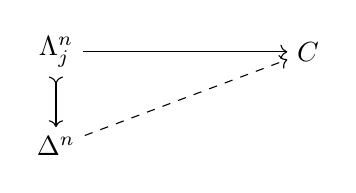
\begin{tikzpicture}[auto]
\node (a) at (0, 1.2) {$\Lambda^n_j$};
\node (x) at (3.2, 1.2) {$C$};
\node (b) at (0, 0) {$\Delta^n$};  
\draw[->] (a) to node {} (x);
\draw[>->] (a) to node {} (b);
\draw[->, dashed] (b) to node[swap] {} (x);
\end{tikzpicture}
\end{center}

\subsection{2-crossed modules}

We now define the notion of a 2-crossed module. Our definition differs slightly from that given in \cite{MartinsPicken2011}. In particular, we use the notation ${}^a b$ for the right action, instead of writing it as  $a \triangleright b$.


%\definton of 2-crossed moudule
A \textbf{2-crossed module} is given by a complex of groups:
\[
L \xrightarrow{\partial} H \xrightarrow{\partial} G 
\]
together with the following three structures:
\begin{itemize}
  \item a left action of $G$ by automorphisms on both $H$ and $L$ (with the action on $G$ given by conjugation);
  \item a left action of $H$ by automorphisms on $L$ (with the action on $H$ also given by conjugation); and
  \item a function $\{-,-\} : H \times H \rightarrow L$ (called the Peiffer lifting);
\end{itemize}
which are required to satisfy the following ten axioms:
\begin{enumerate}
  \item  $\partial\circ \partial =0$;
  \item  $\partial(^gh)= {^g}\partial(h),\ \partial({^g}l)= {^g}\partial(l),\ \partial(^hl)= {^h}\partial(l)$, for each $g \in G$, $h \in H$, and $l \in L$;
  \item  $^g \{h_2,h_1\} = \{\act{g} h_2, \act{g}h_1\}$, for each $g\in G$ and $h_1,h_2 \in H$;
  \label{pfeq}
  \item $\partial  \{h_2, h_1\} = h_2 h_1 h_2^{-1} \act{\partial h_2}h_1^{-1}$, for each $h_1,h_2 \in H$;
  \item $\act{\del l}l' = l l' l^{-1}$, for each $l,l' \in L$;
\label{2cm_pf_id}
  \item $\{\partial l_2,\partial l_1\} = l_2l_1l_2^{-1}l_1^{-1}$, for each $l_1,l_2 \in L$;
\label{2cm_not_need_pl}
  \item $\{h_3h_2,h_1\}={^{h_3}}\{h_2, h_1\}\{h_3, {^{\partial h_2}}h_1 \}$, for each $h_1,h_2, h_3 \in H$;
  \label{lpl}
  \item $\{h_3,h_2 h_1\}=\{h_3, h_2\} {^{(^{\partial h_3} h_2)}}\{h_3, h_1\}$, for each $h_1,h_2, h_3 \in H$;
  \label{rpl}
  \item ${^h}l = l\{\partial l^{-1}, h \}$, for each $h \in H$, and $l\in L$;
  \label{acthl}
  \item ${^{\partial h}}l = {^h}l\{h, \partial l^{-1} \}$, for each $h\in H$, and $l \in L$; and
  \label{actgl}
  \item $l^{-1} {^{\partial h}}l=\{\partial l^{-1}, h \}\{h, \partial l^{-1} \}$, for each $h \in H$, and $l \in L$.
  \label{2cm_not_need}
\end{enumerate}

\begin{rem}
In our context of 2-crossed modules, property \ref{2cm_not_need} follows from properties \ref{acthl} and \ref{actgl}. Similarly, property \ref{2cm_not_need_pl} can be derived by applying properties \ref{2cm_pf_id} and \ref{acthl} to the expression $\act{\del l_2}l_1$. We include these properties explicitly to emphasize that our structure satisfies the same axioms as standard 2-crossed modules.
\end{rem}

\section{2-crossed modules and simplicial sets}\label{sec-2-crossed module and sset}
Before presenting the definition of 3-crossed modules and proving that the simplicial set associated with a 3-crossed module is a quasi-category, we construct a simplicial set using a 2-crossed module and show that it is a quasi-category. Most of the discussion in this section serves as a simplified case of the 3-crossed module.

Let $W \coloneqq (L \xrightarrow{\partial} H \xrightarrow{\partial} G,\{-,-\} )$ be a 2-crossed module. We construct a simplicial set $M_W$ by the following data:

\begin{itemize}
    \item For each $[n] \in \Delta$, the set $M_W([n])$ consists of all the tuples $(g(-,-), h(-,-,-), l(-,$ $-,-,-))$, where:
    \begin{enumerate}
        \item $g: [n] \times_{\le} [n] \to G$ is a function assigning each ordered pair in $[n]$ to an element of $G$;
        \item $h:[n] \times_{\le} [n] \times_{\le} [n] \to H$ is a function assigning  each ordered triple in $[n]$ to an element of $H$; and
        \item $l: [n] \times_{\le} [n] \times_{\le} [n] \times_{\le} [n] \to L$ is a function assigning each ordered quadruple in $[n]$ to an element of $L$;
    \end{enumerate}
    and the three fuctions $g,h$ and $l$ satisfy the following conditions:
    
	
\begin{enumerate}[label=(\alph*)]
\item for each $i \le j \le k$ in $[n]$, we have the idenntity 
\begin{equation}
g_{ik} = \partial(h_{ijk})g_{jk}g_{ij};
\label{r2-simplex}
\end{equation}
\item for each $i \le j \le k \le m$ in $[n]$, we have the idenntity 
\begin{equation}
\partial (l_{ijkm})  h_{ikm}{^{g_{km}}}h_{ijk} = h_{ijm}h_{jkm};
\label{r3-simplex}
\end{equation}
\item for each $i \le j \le k \le m \le p$ in $[n]$, we have the idenntity 
\begin{equation}
 {^{h_{ijp}}}l_{jkmp}l_{ijmp}{^{h_{imp}}}\left({^{g_{mp}}}l_{ijkm}\right) = l_{ijkp}{^{h_{ikp}}}\{h_{kmp},{^{g_{mp}g_{km}}}h_{ijk} \}^{-1}l_{ikmp};
\label{r4-simplex}
\end{equation}
 \item for each $i \in [n]$, we have $g_{ii} = e_G$;
        
 \item for each $i \le j$ in $[n]$, we have $h_{iij} = h_{ijj} = e_H$; and
        
 \item for each $i \le j \le k$ in $[n]$, we have $l_{iijk} = l_{ijjk} = l_{ijkk} = e_L$.
    \end{enumerate}
    
    Here, we simply denote  $g(i,j)$, $h(i,j,k)$, and $l(i,j,k,m)$ by $g_{ij}$, $h_{ijk}$, and $l_{ijkm}$, respectively.
    
\item For a simplicial operater $\delta : [m] \rightarrow [n]$, we define $M_W(\delta): (M_W)_n \rightarrow (M_W)_m$ as follows: for each $(g,h,l) \in (M_W)_n$, %$M_W(\delta)$,
\[
M_W(\delta)
\begin{pmatrix}
g(-,-)\\
h(-,-,-)\\
l(-,-,-,-)\\
\end{pmatrix}
\coloneqq
\begin{pmatrix}
g(\delta(-),\delta(-))\\
h(\delta(-),\delta(-),\delta(-))\\
l(\delta(-),\delta(-),\delta(-),\delta(-))\\
\end{pmatrix}
.\]
\end{itemize}

\noindent
We will show that simplicial set $M_W$ is a quasi-category in the following theorem.

\begin{theorem}\label{2cm and qusi}
Let $W \coloneqq (L \xrightarrow{\partial} H \xrightarrow{\partial} G,\{-,-\} )$ be a 2-crossed module. Then the simplicial set $M_W$ is a quasi-category.
\end{theorem}


In order to prove Theorem~\ref{2cm and qusi}, we need the following two lemmas.

\begin{lemma}
\label{lemma1}
Let \( W \coloneqq (L \xrightarrow{\partial} H \xrightarrow{\partial} G, \{-,-\}) \) be a 2-crossed module. For any \( n \ge 1 \) and any inner horn \( \Lambda^n_j \), let \( \phi \in \operatorname{Hom}(\Lambda^n_j, M_W) \). Then, for any \( m \ge 1 \) and any \( f \in (\Lambda^n_j)_m \), the following identity holds:
\[
\phi_m(f) 
\coloneqq
\begin{pmatrix}
\phi^g_m(f)(-,-) \\
\phi^h_m(f)(-,-,-) \\
\phi^l_m(f)(-,-,-,-)
\end{pmatrix}
=
\begin{pmatrix}
\phi^g_1(f(-,-))(0,1) \\
\phi^h_2(f(-,-,-))(0,1,2) \\
\phi^l_3(f(-,-,-,-))(0,1,2,3)
\end{pmatrix}.
\]
\end{lemma}

For any $m\ge 1$, any $k+1$ integers  \( 0\le x_0 \le x_1 \le \dots \le x_k \le m\)
and
each \( f \in (\Lambda^n_j)_m \),
clearly there exists a function \(f' \in (\Lambda^n_j)_k \) 
satisfying $f'(i) = f(x_i)$ for each $i$, $0\leq i\leq k$.
We renamed such a function $f'$ to  \( f(x_0, x_1, \dots, x_k) \in (\Lambda^n_j)_k \) 
for improving readability.

\begin{proof}
We will prove the case of \( \phi^l_m(f)(i,j,k,p) = \phi^l_3(f(i,j,k,p))(0,1,2,3) \). The other components \( \phi^g_m \) and \( \phi^h_m \) can be handled in the same way.

Let \( \phi \in \operatorname{Hom}(\Lambda^n_j, M_W) \) and let \( f \in (\Lambda^n_j)_m \) for \( m \ge 1 \). We consider \( \phi^l_m(f)(i,j,k,p) \) for \( i \le j \le k \le p \) in \( [m] \).

Define a function \( \langle ijkp \rangle : [3] \to [m] \) by:
\[
\langle ijkp \rangle(x) \coloneqq
\begin{cases}
i & \text{if } x = 0, \\
j & \text{if } x = 1, \\
k & \text{if } x = 2, \\
p & \text{if } x = 3.
\end{cases}
\]
Using the defining property of a natural transformation $\phi$, we obtain the following commutative diagram:
\begin{center}
\begin{tikzpicture}[scale=4] 
       \coordinate (0) at (0,0); 
 	\coordinate (1) at (1,0); 
	 \coordinate (2) at (0,-1);
	 \coordinate (3) at (1,-1);
	 \draw (0) node[] {$(\Lambda^n_j)_m$};
	 \draw (1) node[] {$(M_W)_m$};
	 \draw (2) node[] {$(\Lambda^n_j)_3$};
	 \draw (3) node[] {$(M_W)_3$};
 \draw[->]  ($(0)+(0.2,0)$) to  ($(1)+(-0.2,0)$);
  \draw[->]  ($(2)+(0.2,0)$) to ($(3)+(-0.2,0)$);
  \draw[->]  ($(0)+(0,-0.2)$) to ($(2)+(0,0.2)$);
\draw[->]  ($(1)+(0,-0.2)$) to ($(3)+(0,0.2)$);
 \draw (0.5,0) node[above] {$\phi_m$};  
 \draw (0.5,-1) node[below] {$\phi_3$};
 \draw (0,-0.5) node[left] {$(\Lambda^n_j)(\langle ijkp\rangle)$};
 \draw (1,-0.5) node[right] {$M_W(\langle ijkp\rangle)$};
 \draw[<-] (0.6,-0.5) arc[start angle=0, end angle=-270, radius=0.1];
\end{tikzpicture}
\end{center}
	 

From this diagram, we obtain
\begin{align*}
\phi^l_m(f)(i,j,k,p) 
&= \left(M_W(\langle ijkp \rangle)\left(\phi_m (f)\right)\right)(0,1,2,3) \\
&= \left( \phi_3\left(\Lambda^n_j (\langle ijkp\rangle)(f) \right) \right)(0,1,2,3) \\
&= \phi^l_3 (\langle f(i)f(j)f(k)f(p) \rangle)(0,1,2,3) .
\end{align*}
This completes the proof.
\end{proof}

By examining the proof above, we observe that the argument does not depend on the fact that we are using an inner horn \( \Lambda^n_j \). The same reasoning applies when \( \Lambda^n_j \) is replaced by the standard simplex \( \Delta^n \). For this reason, we obtain the following corollary.

\begin{corollary}
Let \( W \coloneqq (L \xrightarrow{\partial} H \xrightarrow{\partial} G, \{-,-\}) \) be a 2-crossed module. For any \( n \ge 1 \) and any standard simplex \( \Delta^n \), let \( \phi \in \operatorname{Hom}( \Delta^n, M_W) \). Then, for any \( m \ge 1 \) and any \( f \in (\Delta^n)_m \), the following identity holds:
\[
\phi_m(f) 
\coloneqq
\begin{pmatrix}
\phi^g_m(f)(-,-) \\
\phi^h_m(f)(-,-,-) \\
\phi^l_m(f)(-,-,-,-)
\end{pmatrix}
=
\begin{pmatrix}
\phi^g_1(f(-,-))(0,1) \\
\phi^h_2(f(-,-,-))(0,1,2) \\
\phi^l_3(f(-,-,-,-))(0,1,2,3)
\end{pmatrix}.
\]
\end{corollary}

By using Lemma~\ref{lemma1}, we can conclude that any $\phi \in \operatorname{Hom}(\Lambda^n_j, M_W)$ is determined by $\phi_1, \phi_2$, and $\phi_3$.
Let $\psi \in \operatorname{Hom}(\Lambda^2_1, M_W)$. Then, it is possible that $\psi^l_3(\langle 0111 \rangle)(0,1,2,3)$ occurs, by Lemma~\ref{lemma1}.
However, we want $\psi$ to be determined solely by $\psi_1$, since $\Lambda^2_1$ contains only 1-simplices.

The following lemma resolves the issue that arises when degenerate simplices are involved.

\begin{lemma}
\label{lemma2}

Let \( W \coloneqq (L \xrightarrow{\partial} H \xrightarrow{\partial} G, \{-,-\}) \) be a 2-crossed module. For any \( n \ge 1 \) and any inner horn \( \Lambda^n_j \), let \( \phi \in \operatorname{Hom}(\Lambda^n_j, M_W) \). Then for any map $ \langle a_0 \dots a_i a_{i+1}\dots a_m  \rangle \in (\Lambda^n_j)_m $ with \(1\le m \le 3 \), the following equation holds whenever $a_i = a_{i+1}$ for any $0\le i  \le m-1$:
\[
\phi_m (\langle a_0 \dots a_i a_{i+1}\dots a_m \rangle) (0,1,\dots, m) = \phi_{m-1} (\langle a_0 \dots a_i \hat{a}_{i+1}\dots a_m \rangle) (0,1,\dots, i,i,\dots,m-1)
\]
where the $\hat{a}_{i+1}$ indicates that ${a}_{i+1}$ omitted.

\end{lemma}

\begin{proof}
This follows directly from Lemma~\ref{lemma1}.
\end{proof}


Now we can prove Theorem~\ref{2cm and qusi}.

\begin{proof}[of Theorem~\ref{2cm and qusi}]
What we need to prove is that every \( \psi \in \operatorname{Hom}(\Lambda^n_j, M_W) \) can be extended to  
\( \tilde{\psi} \in \operatorname{Hom}(\Delta^n, M_W) \) for all \( n \geq 2 \) and \( 0 < j < n \).  
By using Lemmas~\ref{lemma1} and~\ref{lemma2}, and properties (d)–(e) of \( M_W \),  
to determine \( \tilde{\psi} \in \operatorname{Hom}(\Delta^n, M_W) \),  
it suffices to construct  
$
\tilde{\psi}_2(\langle ij \rangle)(0,1), \ 
\tilde{\psi}_3(\langle ijk \rangle)(0,1,2), \quad \text{and} \ 
\tilde{\psi}_4(\langle ijkp \rangle)(0,1,2,3)
$
for each \( 0 \leq i \leq j \leq k \leq p \leq n \).  
There are four cases to consider.

%\begin{enumerate}[label=(\roman*)]
\begin{enumerate}
\item ${\rm Hom}(\Lambda^2_1, M_W)$ to ${\rm Hom}(\Delta^2, M_W)$

The images of $\Lambda^2_1$  and $\Delta^2$ are illstrated in Figrue~\ref{fig:l^2_1}.

\begin{figure}[htbp]
\begin{center}
\begin{tikzpicture}[scale=2]
\label{fig:l^2_1}
\coordinate[label=left:0]  (0) at (0,0);
\coordinate[label=above:1]  (1) at (0.75,1);
\coordinate[label=right:2]  (2) at (1.5,0);
\draw (0) -- (1);
\draw (1) -- (2);
\draw (0.75,-0.2) node [below] {$\Lambda^2_1$};

\begin{scope}[xshift=3.0cm]
\coordinate[label=left:0]  (0) at (0,0);
\coordinate[label=above:1]  (1) at (0.75,1);
\coordinate[label=right:2]  (2) at (1.5,0);
\draw (0) -- (1);
\draw (1) -- (2);
\draw (0) -- (2);
\draw (0.75,-0.2) node [below] {$\Delta^2$};
\end{scope}

\end{tikzpicture}
\end{center}
\caption{$\Lambda^2_1$ and $\Delta^2$}
\label{l^2_1}
\end{figure}


For any \( \psi \in \operatorname{Hom}(\Lambda^2_1, M_W) \), the map \( \psi \) is determined by  
\( \psi_1(\langle 01 \rangle)(0,1) \) and \( \psi_1(\langle 12 \rangle)(0,1) \).
To extend \( \psi \) to \( \tilde{\psi} \in \operatorname{Hom}(\Delta^2, M_W) \),  
it suffices to construct  
\( \tilde{\psi}_1(\langle 02 \rangle)(0,1) \) and \( \tilde{\psi}_2(\langle 012 \rangle)(0,1,2) \).
We construct these as follows:  
\begin{align*}
\tilde{\psi}_1(\langle 01 \rangle)(0,1) &\coloneqq {\psi}_1(\langle 01 \rangle)(0,1)\\
\tilde{\psi}_1(\langle 12 \rangle)(0,1) &\coloneqq {\psi}_1(\langle 12 \rangle)(0,1)\\
\tilde{\psi}_1(\langle 02 \rangle)(0,1) &\coloneqq \psi_1(\langle 12\rangle)(0,1)\cdot \psi_1(\langle 01\rangle)(0,1)\\
\tilde{\psi}_2(\langle 012 \rangle)(0,1,2) &\coloneqq e_H
.
\end{align*}
It is easy to see that \( \tilde{\psi} \) is an element of \( \operatorname{Hom}(\Delta^2, M_W) \).


\item ${\rm Hom}(\Lambda^3_i, M_W)$ to ${\rm Hom}(\Delta^3, M_W)$ for $1 \le i \le 2$

We will prove the case \( i = 2 \). The case \( i = 1 \) can be handled in a similar manner.
By comparing \( \Lambda^3_2 \) and \( \Delta^3 \), the difference lies in the presence of the 2-simplex \( \langle 013 \rangle \) and the 3-simplex \( \langle 0123 \rangle \).  
To extend a map \( \psi \in \operatorname{Hom}(\Lambda^3_2, M_W) \) to  
\( \tilde{\psi} \in \operatorname{Hom}(\Delta^3, M_W) \),  
we need to construct $\tilde{\psi}_2(\langle 013 \rangle)(0,1,2)$ and $\tilde{\psi}_3(\langle 0123 \rangle)(0,1,2,3)$. We construct them as follows:
\begin{align*}
\tilde{\psi}_1(\langle ij \rangle)(0,1) &\coloneqq {\psi}_1(\langle ij \rangle)(0,1) \ {\rm\ for\ all\ 0\le i\le j \le 3}\\
\tilde{\psi}_2(\langle 012 \rangle)(0,1,2) &\coloneqq {\psi}_2(\langle 012 \rangle)(0,1,2) \\
\tilde{\psi}_2(\langle 123 \rangle)(0,1,2) &\coloneqq {\psi}_2(\langle 123 \rangle)(0,1,2) \\
\tilde{\psi}_2(\langle 023 \rangle)(0,1,2) &\coloneqq {\psi}_2(\langle 023 \rangle)(0,1,2) \\
\tilde{\psi}_2(\langle 013 \rangle)(0,1,2) &\coloneqq h_{023}{^{g_{23}}}h_{012}h^{-1}_{234}\\
\tilde{\psi}_3(\langle 0123 \rangle)(0,1,2,3) &\coloneqq e_L.
\end{align*}

%&\coloneqq \psi_2(\langle 023 \rangle)(0,1,2)\cdot {^{\psi_1(\langle 23 \rangle)(0,1)}}\psi_2(\langle 012 \rangle)(0,1,2) \cdot  \psi^{-1}_2(\langle 234 \rangle)(0,1,2) \\


Here, we write \( g_{ij} \) and \( h_{ijk} \) as follows:
\begin{align*}
g_{ij}&\coloneqq \psi_1(\langle ij \rangle)(0,1)\\
h_{ijk}&\coloneqq \psi_2(\langle ijk \rangle)(0,1,2).
\end{align*}

\item ${\rm Hom}(\Lambda^4_i, M_W)$ to ${\rm Hom}(\Delta^4, M_W)$ for $1 \le i \le 3$

We will prove the case \( i = 3 \). The cases \( i = 1, 2 \) can be handled in a similar manner.
The difference between \( \Lambda^4_3 \) and \( \Delta^4 \) is the presence of the 3-simplex \( \langle 0124 \rangle \) and the 4-simplex \( \langle 01234 \rangle \).
By the properties of \( M_W \), to extend \( \psi \in \operatorname{Hom}(\Lambda^4_3, M_W) \) to  
\( \tilde{\psi} \in \operatorname{Hom}(\Delta^4, M_W) \),  
it suffices to construct only  $\tilde{\psi}_3(\langle 0124 \rangle)(0,1,2,3)$.
The following construction will be sufficient:  
\begin{align*}
\tilde{\psi}_1(\langle ij \rangle)(0,1) &\coloneqq {\psi}_1(\langle ij \rangle)(0,1)  \text{ for all } 0\le i\le j \le 3,\\
\tilde{\psi}_2(\langle ijk \rangle)(0,1,2) &\coloneqq {\psi}_2(\langle ijk \rangle)(0,1,2)  \text{ for all }  0\le i\le j \le k\le 4,\\
\tilde{\psi}_3(\langle 1234 \rangle)(0,1,2) &\coloneqq {\psi}_3(\langle 1234 \rangle)(0,1,2),\\
\tilde{\psi}_3(\langle 0234 \rangle)(0,1,2) &\coloneqq {\psi}_3(\langle 0234 \rangle)(0,1,2),\\
\tilde{\psi}_3(\langle 0134 \rangle)(0,1,2) &\coloneqq {\psi}_3(\langle 0134 \rangle)(0,1,2),\\
\tilde{\psi}_3(\langle 0123 \rangle)(0,1,2) &\coloneqq {\psi}_3(\langle 0123 \rangle)(0,1,2), \text{ and }\\
\tilde{\psi}_3(\langle 0123 \rangle)(0,1,2) &\coloneqq {}^{h_{014}} l_{1234} \, l_{0134} \, {}^{h_{034}}\left( {}^{g_{34}} l_{0123}\right) \, l^{-1}_{0234} \, {}^{h_{024}} \{ h_{234}, {}^{g_{34} g_{23}} h_{012} \}.
\end{align*}
Here, we write \( g_{ij} \), \( h_{ijk} \), and \( l_{ijkm} \)  as follows: 
\begin{align*}
g_{ij}&\coloneqq \psi_1(\langle ij \rangle)(0,1),\\
h_{ijk}&\coloneqq \psi_2(\langle ijk \rangle)(0,1,2), \text{ and}\\
l_{ijkm}&\coloneqq \psi_3(\langle ijkm \rangle)(0,1,2,3).
\end{align*}

\item ${\rm Hom}(\Lambda^n_i, M_W)$ to ${\rm Hom}(\Delta^n, M_W)$ for $5\le n$ and $1 \le i \le n-1$

The difference between \( \Lambda^n_i \) and \( \Delta^n \) is the presence or absence of the \((n-1)\)-simplex \( \langle 01 \dots \hat{i} \dots n \rangle \) and the \( n \)-simplex \( \langle 01 \dots n \rangle \).
By the properties of \( M_W \), any \( \psi \in \operatorname{Hom}(\Lambda^n_i, M_W) \) can be extended directly to  
\( \tilde{\psi} \in \operatorname{Hom}(\Delta^n, M_W) \) as follows:
\begin{align*}
\tilde{\psi}_1(\langle ij \rangle)(0,1) &\coloneqq {\psi}_1(\langle ij \rangle)(0,1)  \text{ for all }  0\le i\le j \le 3, \\
\tilde{\psi}_2(\langle ijk \rangle)(0,1,2) &\coloneqq {\psi}_2(\langle ijk \rangle)(0,1,2)  \text{ for  all } 0\le i\le j \le k\le 4, \text{ and}\\
\tilde{\psi}_3(\langle ijkm \rangle)(0,1,2,3) &\coloneqq {\psi}_3(\langle ijkm \rangle)(0,1,2,3) \text{ for all } 0\le i\le j \le k\le m \le n.
\end{align*}
\end{enumerate}
This completes the proof.
\end{proof}

\section{3-crossed modules and simplicial sets}\label{sec-3-crossed module and sset}

In this section, we define a 3-crossed module. After defining the notion of a 3-crossed module, we construct a simplicial set associated with it and prove that this simplicial set is a quasi-category.

A 3-crossed module involves four distinct groups, four types of actions, and six types of liftings.

\begin{dfn}{(3-crossed module)}
\label{d3cm}
Let $G,H,L,M$ be groups. A {\bf 3-crossed module} is a complex of groups:
\[
 M\xrightarrow{\partial}L \xrightarrow{\partial} H \xrightarrow{\partial} G 
\]
together with the following structures:
\begin{itemize}
  \item a left action of $G$ by automorphisms on  $H$, $L$ and $M$ (with the action on $G$ given by conjugation),
  \item a left action of $H$ by automorphisms on $L$ and $M$ (with the action on $H$ also given by conjugation),
  \item a left action of $L$ by automorphisms on $M$(with the action on $L$ also given by conjugation),
  \item a function $\{-,-\} : H \times H \rightarrow L$ (called the Peiffer lifting),
  \item a function $\{-,-,-\} : H \times H \times H  \rightarrow M$ (called the Left-Homanian),
  \item a function $\{-,-,-\}' : H \times H \times H  \rightarrow M$ (called the Right-Homanian),
  \item a function $\{-,-\}_{HL} : H \times L \rightarrow M$ (called the HL-Peiffer lifting),
  \item a function $\{-,-\}'_{HL} : H \times L \rightarrow M$ (called the HL'-Peiffer lifting),  and
  \item a function $\{-,-\}_{LL} : L \times L \rightarrow M$ (called the LL-Peiffer lifting),         
\end{itemize}
which are required to satisfy the following axioms:
\begin{enumerate}
  \item Each $\partial$ is homomorphism.
  \item  $\partial\circ \partial =0$.
  \item For each $g \in G$, $h \in H$, $l \in L$, and $m \in M$,
  \begin{align*}
\left\{
    \begin{aligned}
    & \partial({}^gh)= {{}^g}\partial(h) \\
    & \partial({}^gl)= {{}^g}\partial(l)  \\
    & \partial({}^gm)= {{}^g}\partial(m) .
    \end{aligned}
\right.
\end{align*}
  \item For each $h \in H$, $l \in L$, and $m \in M$,
  \begin{align*}
\left\{
    \begin{aligned}
    & \partial({}^hl)= {{}^h}\partial(l)  \\
    & \partial({}^hm)= {{}^h}\partial(m) .
    \end{aligned}
\right.
\end{align*}
  \item For each $l \in L$ and $m \in M$,
\[
\partial({}^lm)= {{}^l}\partial(m).
\]
  \item For each $g\in G$ and $h_1,h_2 \in H$,
  \[
   ^g \{h_2,h_1\} = \{^g h_2,^g h_1\} .
  \]
  \item For each $g\in G$ and $h_1,h_2,h_3 \in H$,
  \begin{align*}
\left\{
    \begin{aligned}
   &{}^g \{h_3,h_2,h_1\} = \{{}^g h_3,{}^g h_2, {}^g h_1\}\\
   &{}^g \{h_3,h_2,h_1\}' = \{{}^g h_3,{}^g h_2, {}^g h_1\}'. 
    \end{aligned}
\right.
\end{align*}
  \item For each $g\in G$ and $l_1,l_2 \in L$,
  \begin{align*}
{}^g \{l_2,l_1\}_{LL} = \{{}^g l_2,{}^g l_1\}_{LL}.
\end{align*}
 \item For each $h\in H$ and $l_1,l_2 \in L$,
  \begin{align*}
{}^h \{l_2,l_1\}_{LL} = \{{}^h l_2,{}^h l_1\}_{LL}.
\end{align*}

\item For each $l\in L$ and $m \in M$,
 \[
 \act{\del l}m = \act{l}m\{l,\partial m^{-1}\}_{LL}  .
 \] 
\label{act_u_ll_dellm}
\item For each $l\in L$ and $m \in M$,
 \[
 \act{l}m = m\{\partial m^{-1}, l\}_{LL} .
 \] 
\label{act_u_ll_lm}
  \item For each $m,m'\in M$,
  \[
  \act{\partial m}m' = mm'm^{-1} .
  \]
\label{act_delm_m_3cm}

  \item For each $h\in H$ and $l \in L$,
  \[
  \partial\{h,l\}_{HL}\act{h}l = l\{\partial l^{-1},h\}.
  \]
  \label{dhl}
  
    \item For each $h\in H$ and $l \in L$,
  \[
  \partial\{h,l\}'_{HL}\act{\partial h}l = \act{h}l\{h,\partial l^{-1}\}.
  \]
\label{dhlp}

  \item For each $g\in H$,$h\in H$, and $l \in L$,
  \begin{align*}
\left\{
    \begin{aligned}
{}^g \{h,l\}_{HL} &= \{{}^g h, {}^g l\}_{HL}\\
{}^g \{h,l\}_{HL}' &= \{{}^g h, {}^g l\}_{HL}'.
    \end{aligned}
\right.
\end{align*}

  
  \item For each $h\in H$ and $m \in M$,
 \[
 \act{h}m = m\{h,\partial m^{-1}\}_{HL}  .
 \] 
\label{act_h_m_3cm}

 \item For each $l,l'\in L$,
 \[
\partial\{l,l'\}_{LL}\act{\partial l}l' = ll'l^{-1}.
 \]
 \label{dll}
  \item  For each $h_1,h_2, h_3 \in L$,
  \[
  \{l_3l_2,l_1\}_{LL}={^{l_3}}\{l_2, l_1\}_{LL}\{l_3, {^{\partial l_2}}l_1 \}_{LL}.
  \] 
  \label{lll}
  \item For each $l_1,l_2, l_3 \in L$,
  \[
  \{l_3,l_2 l_1\}_{LL}=\{l_3, l_2\}_{LL} {^{(^{\partial l_3} l_2)}}\{l_3, l_1\}_{LL}.
  \] 
  \label{rll}
  \item For each $h\in H$ and $m \in M$,
 \[
 \act{\partial h}m = \act{h}m\{h,\partial m^{-1}\}'_{HL}  .
 \] 
 \label{dhmnl}
  \item For each $h_1,h_2,h_3 \in H$,
\[
\{h_3h_2,h_1\} = \partial\{h_3,h_2,h_1\}\ {{}^{h_3}\{h_2,h_1\}}\{h_3, {}^{\partial h_2}h_1\}.
\]  
\label{dhmnr}
  \item For each $h_1,h_2,h_3 \in H$,
\[
\{h_3,h_2h_1\} = \partial\{h_3,h_2,h_1\}' \{h_3,h_2\}{}^{\left({}^{\partial h_3}h_2\right) }\{h_3, h_1\}.
\]
  \item For each $h_1,h_2 \in H$ and $l \in L$,
\[
\{h_2h_1,l\}_{HL} = \act{l}\{\partial l^{-1},h_2,h_1\}'\{h_2,l\}_{HL} \act{h_2}\{h_1,l\}_{HL}  .
\]  
\label{rl:hhl}

  \item For each $h \in H$ and $l_1,l_2 \in L$,
\[
\{h,l_2l_1\}_{HL} = \act{l_2l_1}\{\partial l_1^{-1},\partial l_2^{-1},h\}\act{l_2l_1}\{l_1^{-1},\{\partial l_2^{-1},h\}\}_{LL} ^{-1}\{h,l_2\}_{HL} \act{\left(\act{h}l_2\right)}\{h,l_1\}_{HL}  .
\] 
  \item For each $h_1,h_2 \in H$ and $l \in L$,
\[
\{h_2h_1,l\}'_{HL} = \act{\left(\act{h_2h_1}l\right)}\{h_2,h_1,\partial l^{-1}\}\act{h_2}\{h_1,l\}'_{HL}\{h_2,\act{\partial h_1}l\}'_{HL} .
\]   
  \item For each $h \in H$ and $l_1,l_2 \in L$,
\[
\{h,l_2l_1\}'_{HL} = \act{\left(\act{h}(l_2l_1)\right)}\{h,\partial l_1^{-1},\partial l_2^{-1}\}'\act{\left(\act{h}l_2\right)}\{h,l_1\}'_{HL}\act{\left(\act{h}l_2\act{\partial h}l_1\right)}\{\act{\partial h}l_1^{-1},\{h,\partial l_2^{-1}\}\}_{LL}^{-1}\{h,l_1\}'_{HL}  .
\] 
\label{rrHL}
 \item For each $h_1,h_2,h_3,h_4 \in H$,
 \[
 \{h_4h_3,h_2,h_1\}\act{\left(\act{h_4h_3}\{h_2,h_1\}\right)}\{h_4,h_3,\act{\partial h_2}h_1\} = \{h_4,h_3h_2,h_1\}\act{h_4}\{h_3,h_2,h_1\} .
 \]
  \label{lhmnr}
  
  \item For each $h_1,h_2,h_3,h_4 \in H$,
 \[
\{h_4,h_3h_2,h_1\}'\{h_4,h_3,h_2\}' = \{h_4,h_3,h_2h_1\}'\act{\{h_4,h_3\}}(\act{\left(\act{\partial h_4}h_3\right)}\{h_4,h_2,h_1\}') .
 \]
 \label{rhmnr}

    \item For each $h_1,h_2,h_3,h_4 \in H$,
 \begin{align*}
&\{h_4,h_3,h_2h_1\}\act{\left(\act{h_4}\{h_3,h_2h_1\}\right)}\{h_4,\act{\partial h_3}h_2,\act{\partial h_3}h_1\}'\act{h_4}\{h_3,h_2,h_1\}' \\
  &= \{h_4h_3,h_2,h_1\}'\act{\{h_4h_3,h_2\}}(\act{\act{\partial (h_4h_3)}h_2}\{h_4,h_3,h_1\})\{h_4,h_3,h_2\} \\
   &\hspace{1em}\times\act{\left(\act{h_4}\{h_3,h_2\}\right)}\{\{h_4,\act{\partial h_3}h_2\},\act{\left(\act{\partial(h_4h_3)}h_2h_4\right)}\{h_3,h_1\}\}_{LL}.
\end{align*}
 \label{lrhmnr}
 
 %--------------
  \item For each $h_1,h_2,h_3 \in H$,
  \label{yanBt}
 \begin{align}
  \nonumber
 &\act{\act{h_3}\{h_2,h_1\}}(\{h_3,\act{\partial h_2}h_1,h_2\}'^{-1}\{h_3,\partial\{h_2,h_1\}^{-1},h_2h_1\}')\{h_3,\{h_2,h_1\}\}' \\
  \nonumber
  \hspace{1em} &\{\act{\partial h_3}\{h_2,h_1\},\act{\partial\act{\partial h_3}\{h_2,h_1\}^{-1}}\{h_3,h_2h_1\}\}\{h_3,h_2,h_1\}' \\
  \nonumber
  &= \{h_3,h_2,h_1\}^{-1}\act{\{h_3h_2,h_1\}}\{\act{\partial(h_3h_2)}h_1,\{h_3,h_2\}\}^{-1}\{\{h_3,h_2\},\act{\partial\{h_3,h_2\}^{-1}}\{h_3h_2,h_1\}\}^{-1} \\
  \nonumber
  &\hspace{1em} \act{\{h_3,h_2\}}(\{\partial\{h_3,h_2\}^{-1},h_3h_2,h_1\}^{-1}\{\act{\partial h_3}h_2,h_3,h_1\})
\end{align}
 
 
 
 %-------------
 
 
 
    \item For each $l,l' \in L$,
    \[
    \act{l}\{\partial l',l^{-1}\}_{HL}\act{ll'l^{-1}l'^{-1}}\{l',l\}_{LL}= \act{\left(\act{\partial l}l'\right)}\{\partial l,l'^{-1}\}'_{HL}\{l,l'\}^{-1}_{LL}.
    \]
     \item For each $l\in L$ and $m \in M$,
    \[
    \{\partial m,l\}_{LL}\{l,\partial m\}_{LL} = \{\partial l,\partial m\}_{HL} = \{\partial l,\partial m\}'^{-1}_{HL}.
    \]
    \label{rllandhl}
        \item For each $m,m' \in M$,
    \[
    \{\partial m,\partial m'\}_{LL} = mm'm^{-1}m'^{-1}.
    \]   
\label{3cm_not_need}
\end{enumerate}
\end{dfn}

\begin{rem}
Properties \ref{rllandhl} and \ref{3cm_not_need} can be derived from the other axioms of a 3-crossed module. Specifically, property \ref{rllandhl} is obtained by applying properties \ref{act_u_ll_dellm} and \ref{act_u_ll_lm} to the term $\act{\del l}m$, along with property \ref{act_h_m_3cm} in $\act{\del l}m$ and property \ref{dhmnl} in $\act{\del \circ \del l}m$. Similarly, property \ref{3cm_not_need} follows from properties \ref{act_u_ll_lm} and \ref{act_delm_m_3cm} applied to $\act{\del m'}m$. We include these properties explicitly for the reader's convenience.
\end{rem}

There are six types of liftings. One is the normal Peiffer lifting. The LL-Peiffer lifting corresponds to the normal Peiffer lifting for the complex of groups \( M \xrightarrow{\partial} L \xrightarrow{\partial} H \).
The HL-Peiffer lifting, HL'-Peiffer lifting, and the left and right Homanian are new types of liftings that arise specifically in 3-crossed modules.
As can be seen in the 3-crossed module property~\ref{dhl}, the HL-Peiffer lifting is a twisted version of the 2-crossed module property~\ref{acthl}. According to the 3-crossed module property~\ref{dhlp}, the HL'-Peiffer lifting is a twist of the 2-crossed module property~\ref{actgl}.
The left Homanian corresponds to a twist of the relation in the 2-crossed module property~\ref{lpl}, while the right Homanian corresponds to a twist of the relation in property~\ref{rpl}.

Some of the relations in a 3-crossed module can be understood through diagrams that can be described in the language of category theory.  
See Appendix~\ref{app_dia_3cm} for details.

%start lemma
We investigate the behavior of liftings when one of the arguments is the unit element.
The following lemma describes this situation.
\begin{lemma}
\label{lemma_of_unit_element}
Let $G,H,L,M$ be groups, and let
$
 M\xrightarrow{\partial}L \xrightarrow{\partial} H \xrightarrow{\partial} G 
$ be 3-crossed module. Then the six types of liftings satisfy the following equations:
\begin{align}
\{h_2, h_1\}
  &= e_L
  && \text{if $h_2 = e_H$ or $h_1 = e_H$,}
  \label{eq:einpl} \\
 \{l_2, l_1\}
  &= e_M
  && \text{if $l_2 = e_L$ or $l_1 = e_L$,}
  \label{eq:einll} \\
\{h_3, h_2, h_1\}
  &= \{h_3, h_2, h_1\}' = e_M
  && \text{if $h_3 = e_H$ or $h_2 = e_H$ or $h_1 = e_H$,}
  \label{eq:einhmn} \\
\{h, l\}_{HL}
  &= \{h, l\}'_{HL} = e_M
  && \text{if $h = e_H$ or $l = e_L$.}
  \label{eq:einhl}
\end{align}
Here, $e_X$ denotes the unit element of the group $X$. 
\end{lemma}
\begin{proof}
Equation~(\ref{eq:einll}) follows from Properties \ref{lll} and \ref{rll} of a 3-crossed module applied to $\{e_L e_L, l\}_{LL}$ and $\{l, e_L e_L\}_{LL}$. Indeed,
\begin{equation}
\begin{aligned}
\{e_L e_L , l\}_{LL} &= \{e_L  , l\}_{LL}\{e_L , l\}_{LL},\\
\{l, e_L e_L \}_{LL} &= \{l, e_L\}_{LL} \{l, e_L\}_{LL}.
\end{aligned}
\label{p_einll}
\end{equation}

We next show that, for each $h\in H$,
\begin{equation}
\begin{aligned}
\{e_H, e_H, h\} = e_M,\\
\{h, e_H, e_H\}' = e_M.
\label{hyp_of_unit}
\end{aligned}
\end{equation}
Equation~(\ref{hyp_of_unit}) is obtained by computing $\act{h}(mm')$ and $\act{\del h}(mm')$ and then setting $m=m'=e_M$. We compute $\act{h}(mm')$ as follows:
\begin{align}
  \nonumber
  \act{h}(mm') &= mm'\{h,\partial (mm')^{-1}\}_{HL} \\
  \nonumber
  &= mm'\act{\partial (mm)'^{-1}}\{e_H,e_H,h\}\act{\partial (mm')^{-1}}\{\partial m,\{e_H,h\}\}_{LL}^{-1}\{h,\partial m'^{-1}\}_{HL}\act{\partial \act{h}m'^{-1}}\{h,\partial m^{-1}\}_{HL} \\
  \nonumber
  &= \{e_H,e_H,h\}\{\partial m,\{e_H,h\}\}_{LL}^{-1}mm'\{h,\partial m'^{-1}\}_{HL}\act{\partial \act{h}m'^{-1}}\{h,\partial m^{-1}\}_{HL} \\
  \label{eq:act_hmm}
  &= \{e_H,e_H,h\}\{\partial m,\{e_H,h\}\}_{LL}^{-1}m\act{h}m'\act{\partial \act{h}m'^{-1}}\{h,\partial m^{-1}\}_{HL} \\
  \nonumber
  &= \{e_H,e_H,h\}\{\partial m,\{e_H,h\}\}_{LL}^{-1}m\{h,\partial m^{-1}\}_{HL}\act{h}m' \\
  \nonumber
  &= \{e_H,e_H,h\}\{\partial m,\{e_H,h\}\}_{LL}^{-1}\act{h}m\act{h}m'.
\end{align}
Similarly, $\act{\del h}(mm')$ can be computed in an analogous manner:
\begin{align}
  \nonumber
  \act{\partial h}(mm') &= \act{h}(mm')\{h,\partial (mm')^{-1}\}_{HL} ' \\
  \nonumber
  &= \act{h}(mm')\act{\partial \act{h}(mm')^{-1}}\{h,e_H,e_H\}'\act{\partial \act{h}m'^{-1}}\{h,\partial m^{-1}\}_{HL} '\act{\partial (\act{h}m'^{-1}\act{\partial h}m^{-1})}\{\partial m,\{h,e_H\}\}_{LL} ^{-1}\{h,\partial m'^{-1}\}_{HL} ' \\
  \nonumber
  &= \{h,e_H,e_H\}'\act{h}m\{h,\partial m^{-1}\}_{HL}'\act{\partial (\act{\partial h}m^{-1})}\{\partial m,\{h,e_H\}\}_{LL}^{-1}\act{h}m'\{h,\partial m'^{-1}\}_{HL}' \\
  \label{eq:act_gmm}
  &= \{h,e_H,e_H\}'\act{\partial h}m\act{\partial (\act{\partial h}m^{-1})}\{\partial m,\{h,e_H\}\}_{LL}^{-1}\act{\partial h}m'.
\end{align}
Using Equations~(\ref{eq:act_hmm}) and~(\ref{eq:act_gmm}), together with $m=m'=e_M$ and Equation~(\ref{eq:einll}), we obtain Equation~(\ref{hyp_of_unit}).

Next, by substituting the unit element appropriately into Properties \ref{dhmnr}-\ref{rrHL} of a 3-crossed module, we obtain Equations~(\ref{eq:P11h1h})-(\ref{eq:h11h1}):
\begin{align}
  \label{eq:P11h1h}
  e_L &= \partial\{e_H,e_H,h\}\{e_H,h\}, \\
  \label{eq:Ph11h1}
  e_L &= \partial\{h,e_H,e_H\}'\{h,e_H\}, \\
  \label{eq:Pl111l}
  e_M &= \act{l}\{\partial l^{-1},e_H,e_H\}'\{e_H,l\}_{HL}, \\
  \label{eq:11hh1}
  e_M &= \{e_H,e_H,h\}\{h,e_L\}_{HL},  \\
  \label{eq:11Pl1l}
  e_M &= \act{l}\{e_H,e_H,\partial l^{-1}\}\{e_H,l\}'_{HL},  \\
  \label{eq:h11h1}
  e_M &= \{h,e_L,e_L\}'\{h,e_L\}'_{HL}. 
\end{align}
Using Equations~(\ref{hyp_of_unit}) and (\ref{eq:P11h1h})-(\ref{eq:h11h1}), we obtain Equations~(\ref{eq:einpl}) and~(\ref{eq:einhl}) . 

Now, by setting $h_3=h_2=h_1=e_H$ and $h_4=h_3=h_2=e_H$ in Proprety~\ref{lhmnr} of 3-crossed module, we obtain Equations~(\ref{2ulhmn1}) and (\ref{2ulhmn2}), respectively:
\begin{align}
\label{2ulhmn1}
\{h, e_H, e_H \} = e_M,\\ 
\label{2ulhmn2}
\{e_H, h, e_H \} = e_M.
\end{align}
Similarly, setting $h_4=h_3=h_2=e_H$ and $h_4=h_2=h_1=e_H$ in Proprety~\ref{rhmnr} of a 3-crossed module yields Equations~(\ref{2urhmn1}) and (\ref{2urhmn2}), respectively:
\begin{align}
\label{2urhmn1}
\{e_H, h, e_H \}' = e_M,\\ 
\label{2urhmn2}
\{e_H, e_H, h \}' = e_M.
\end{align}
Using Equations~(\ref{eq:einpl}), (\ref{eq:einll}), (\ref{eq:einhl}), (\ref{hyp_of_unit}), and (\ref{2ulhmn1})-(\ref{2urhmn2}) where necessary, and applying Property~\ref{lhmnr} of a 3-crossed module with $h_4 = h_3 = e_H$ and with $h_3= h_2 = e_H$, we obtain Equation~(\ref{1ulhmn1}) and (\ref{1ulhmn2}), respectively:
  \begin{align}
\label{1ulhmn1}
\{e_H, h_2, h_1 \} = e_M,\\ 
\label{1ulhmn2}
\{h_4, e_H, h_1 \} = e_M.
\end{align}

Similarly, applying Property~\ref{rhmnr} of a 3-crossed module with $h_3 = h_2 = e_H$ and with $h_2= h_1 = e_H$, we obtain Equation~(\ref{1urhmn1}) and (\ref{1urhmn2}), respectively:
\begin{align}
\label{1urhmn1}
\{h_4, e_H, h_1 \}' = e_M,\\ 
\label{1urhmn2}
\{h_4, h_3, e_H \}' = e_M.
\end{align}

Finaly, applying Property~\ref{lrhmnr} of a 3-crossed module with $h_2 = h_1 = e_H$ and with $h_4= h_3 = e_H$, we obtain Equation~(\ref{1ulhmn3}) and (\ref{1urhmn3}), respectively:
\begin{align}
\label{1ulhmn3}
\{h_4, h_3, e_H \} = e_M,\\ 
\label{1urhmn3}
\{e_H, h_2, h_1 \}' = e_M.
\end{align}
This completes the proof.

\end{proof}


These twists naturally appear in the simplicial set associated with a 3-crossed module.  
We now construct the simplicial set associated with a 3-crossed module. This can be done by adding additional structure to the simplicial set associated with a 2-crossed module.

Let \( T \coloneqq  (M \xrightarrow{\partial} L \xrightarrow{\partial} H \xrightarrow{\partial} G) \) be a 3-crossed module.  
The simplicial set \( M_T \) associated with this 3-crossed module consists of the following data:



\begin{itemize}
    \item For each $[n] \in \Delta$, the set $M_W([n])$ consists of quadruples 
    \[ (g(-,-), h(-,-,-), l(-,-,-,-),m(-,-,-,-,-)) ,\]
    where:
    \begin{enumerate}
        \item $g: [n] \times_{\le} [n] \to G$ is a function assigning each ordered pair in $[n]$ to an element of $G$,
        \item $h: [n] \times_{\le} [n] \times_{\le} [n] \to H$ is a function assigning each ordered triple in $[n]$ to an element of $H$,  
        \item $l: [n] \times_{\le} [n] \times_{\le} [n] \times_{\le} [n] \to L$ is a function assigning each ordered quadruple in $[n]$ to an element of $L$, and
        \item $m: [n] \times_{\le} [n] \times_{\le} [n] \times_{\le} [n] \times_{\le} [n] \to M$ is a function assigning each ordered quintuple in $[n]$ to an element of $M$,
    \end{enumerate}
    satisfying the following conditions:
    
	
\begin{enumerate}[label=(\alph*)]
\item for each $i \le j \le k$ in $[n]$, we have the idenntity 
\begin{equation}
g_{ik} = \partial(h_{ijk})g_{jk}g_{ij},
\label{r2-simplex m}
\end{equation}
\item for each $i \le j \le k \le p$ in $[n]$, we have the identity 
\begin{equation}
\partial (l_{ijkp})  h_{ikp}{^{g_{kp}}}h_{ijk} = h_{ijp}h_{jkp},
\label{r3-simplex m}
\end{equation}
\item for each $i \le j \le k \le p \le q$ in $[n]$, we have the idenntity 
\begin{equation}
 \partial(m_{ijkpq}) {^{h_{ijq}}}l_{jkpq}l_{ijpq}{^{h_{ipq}}}\left({^{g_{pq}}}l_{ijkp}\right) = l_{ijkq}{^{h_{ikq}}}\{h_{kpq},{^{g_{pq}g_{kq}}}h_{ijk} \}^{-1}l_{ikpq} ,
\label{r4-simplex m}
\end{equation}
\item for each $i \le j \le k  \le p \le q\le x$ in $[n]$, we have the idenntity 

\label{r5-simplex m}
\begin{equation}
\label{r5-simplex m:eq}
\begin{aligned}
   \act{L_D L_E}M_5 \cdot \act{L_D L_E L_F}M_4 &\cdot M_3 \cdot \act{L_A}M_2 \cdot  \act{L_A L_B L_C} M_1\\
   =
   \act{}M'_{13}
   &\cdot \act{L_K L_N}M'_{12}
   \cdot \act{L_K }M'_{11}
   \cdot \act{L_K L_L}M'_{10}
   \cdot \act{L_K L_L L_M}M'_9\\
  & \cdot \act{}M'_8 
   \cdot \act{L_G L'_I}M'_7
   \cdot \act{L_G L'_I}M'_6
   \cdot \act{L_G }M'_5\\
   &\cdot \act{L_G L_H L_I L_J}M'_4
   \cdot \act{L_G L_H}M'_3
   \cdot \act{}M'_2
   \cdot \act{L_A L_B}M'_1.
   \end{aligned}
   \end{equation}

Here each term will be written as follows:

\noindent
\begin{align*}
     L_A &= \act{h_{ijx}h_{jkx}}l_{kpqx}\\
   L_B &= \act{h_{ijx}}l_{jkqx}\\
   L_C &=l_{ijqx}\\
   L_D &=l_{ijkx}\\
   L_E &=\act{h_{ikx}(\act{g_{kx}}h_{ijk})}l_{kpqx}\\
   L_F &=\act{h_{ikq}}\{h_{kqx}, \act{g_{qx}g_{kq}}h_{ijk} \}^{-1}\\
   M_j &= \act{h_{iqx}}\left(\act{g_{qx}}m_{ijkpq} \right)\\
   M_k &= m_{ijkqx}\\
   M_p &= \{l_{ijkx}, \act{h_{ikx}(\act{g_{kx}}h_{ijk})}l_{kpqx} \}_{L,L}\\
   M_q &= \left\{l_{ikqx},\act{h_{iqx}(\act{g_{qx}}h_{ikq})}\{\act{g_{qx}}h_{kpq},\act{g_{qx}g_{pq}g_{kp}}h_{ijk} \} \right\}^{-1}_{L,L}\\
   M_x &=\act{h_{ikx}}\left(\act{\{h_{kqx},\act{g_{qx}g_{kq}}h_{ijk} \}^{-1}(\act{h_{kqx}}\{\act{g_{qx}}h_{kpq},\act{g_{qx}g_{pq}g_{kp}}h_{ijk} \}^{-1})} \{h_{kqx}, \act{g_{qx}}h_{kpq}, \act{g_{qx}g_{pq}g_{kp}}h_{ijk} \}_L^{-1}\right)
    \end{align*}
   
   \begin{align*}
   L_G &= \act{h_{ijx}}l_{jkpx}\\
   L_H &= \act{h_{ijx}h_{jpx}}\{h_{pqx},\act{g_{qx}g_{pq}}h_{jkp} \}^{-1}\\
   L_I &=L'_I =l_{ijpx}\\
   L_J &=\act{h_{ipx}}\{h_{pqx}, \act{g_{qx}g_{pq}}h_{ijp}\}^{-1} \\
   L_K &=l_{ijkx} \\
   L_L &=\act{h_{ikx}}\{h_{kpx}, \act{g_{px}g_{kp}}h_{ijk} \}^{-1}\\
   L_M &= l_{ikpx} \\
   L_N &= \act{h_{ikx}}\{h_{kpx}h_{pqx}, \act{g_{qx}g_{px}g_{kp}}h_{ijk} \}^{-1}\\
   M'_j &= \{l_{ijqx}, \act{h_{iqx}(\act{g_{qx}h_{ijq}})}(\act{g_{qx}}l_{jkpq}) \}^{-1}_{L,L}\\
   M'_k &= m_{jkpqx}\\
   M'_p &= m_{ijpqx}\\
   M'_q &= \{l_{ipqx}, \act{h_{iqx}(\act{g_{qx}h_{ipq}})}(\act{g_{qx}g_{pq}}l_{ijkp}) \}^{-1}_{L,L}\\
   M'_x &=\{l_{ijpx}, \act{h_{ipx}(\act{g_{px}h_{ijq}})}\{h_{pqx} \act{g_{qx}g_{pq} }h_{jkp}  \}\}_{L,L} \\
   M'_6 &=\act{h_{ipx}}\left(\act{(\act{(\act{g_{px}}h_{ijp})}\{h_{pqx}, \act{g_{qx}g_{pq}}h_{jkp} \}^{-1}\{h_{pqx}, \act{g_{qx}g_{pq}}h_{ijp} \}^{-1} ) }\{h_{pqx}, \act{g_{qx}g_{pq}}h_{ijp},\act{g_{qx}g_{pq}}h_{jkp} \}'^{-1}_{R}  \right)\\
   M'_7 &= \act{  (\act{g_{px}}l_{ijkp}\{h_{pqx}, \act{g_{qx}g_{pq}}(h_{ikp}\act{g_{kp}}h_{ijk}) \}^{-1})      }
  \left(  \act{(\act{h_{pqx}}(\act{g_{qx}g_{pq}}l_{ijkp}))}\{h_{pqx}, \act{g_{qx}g_{pq}}(\del l_{ijkp}),\act{g_{qx}g_{pq}}(h_{ikp}\act{g_{kp}}h_{ijk}) \}\right) \\
  &\ \ \ \ \cdot \act{  (\act{g_{px}}l_{ijkp}\{h_{pqx}, \act{g_{qx}g_{pq}}(h_{ikp}\act{g_{kp}}h_{ijk}) \}^{-1})      }\left(\{h_{pqx}, \act{g_{qx}g_{pq}}l_{ijkp}^{-1}\}'_{HL}
  \right)    \\
  &\ \ \ \ \cdot \{ \act{g_{px}}l_{ijkp}, \{h_{pqx}, \act{g_{qx}g_{pq}}(h_{ikp}\act{g_{kp}}h_{ijk}) \}^{-1}\}_{L,L}\\
     M'_8 &=m_{ijkpx}\\
   M'_9 &= \act{h_{ipx}}\left(\act{(\act{(\act{g_{px}}h_{ikp})}\{h_{pqx}, \act{g_{qx}g_{pq}g_{kp}}h_{ijk} \}^{-1}\{h_{pqx}, \act{g_{qx}g_{pq}}h_{ikp} \}^{-1} ) }\{h_{pqx}, \act{g_{qx}g_{pq}}h_{ikp},\act{g_{qx}g_{pq}g_{kp}}h_{ijk} \}'_{R}  \right)\\
     M'_ji &=\{l_{ikpx}, \act{h_{ipx}(\act{g_{px}}h_{ikp})}\{h_{pqx}, \act{g_{qx}g_{pq}g_{kp}}h_{ijk}\}^{-1} \}_{L,L}^{-1}\\
        M'_jj &=\act{h_{ikx}}\left(\act{\{h_{kpx},\act{g_{px}g_{kp}}h_{ijk} \}^{-1}(\act{h_{kpx}}\{h_{pqx},\act{g_{qx}g_{pq}g_{kp}}h_{ijk} \}^{-1})} \{h_{kpx}, h_{pqx}, \act{g_{qx}g_{pq}g_{kp}}h_{ijk} \}_L^{-1}\right)\\
           M'_jk &=m_{ikpqx}^{-1}\\
           M'_jp &= \act{ \act{(\act{g_{px}}h_{ijk})}l_{kpqx}\{h_{kqx}(\act{g_{qx}}h_{kpq}),\act{g_{qx}g_{pq}g_{kp}}h_{ijk}\}^{-1}l_{kpqx}^{-1}}\{\del l_{kpqx}, h_{kqx}\act{g_{qx}}h_{kpq}, \act{g_{qx}g_{pq}g_{kp}}h_{ijk} \} \\
            &\ \ \ \ \cdot \act{\left(\act{(\act{g_{px}}h_{ijk}) }l_{kpqx}\right)}\left( \act{l_{kpqx}^{-1}}\{l_{kpqx},\{h_{kqx}(\act{g_{qx}}h_{kpq}),\act{g_{qx}g_{pq}g_{kp}}h_{ijkp}  \} \}_{L,L}\cdot \{ \act{g_{kx}}h_{ijk}, l_{kpqx}^{-1}\}_{HL}   \right)
    \end{align*}


 \item For each $i \in [n]$, we have $g_{ii} = e_G$,
        
 \item For each $i \le j$ in $[n]$, we have $h_{iij} = h_{ijj} = e_H$,
        
 \item For each $i \le j \le k$ in $[n]$, we have $l_{iijk} = l_{ijjk} = l_{ijkk} = e_L$.
 
 \item For each $i \le j \le k \le p$ in $[n]$, we have $m_{iijkp} = m_{ijjkp} = m_{ijkkp} = m_{ijkpp}= e_m$.
    \end{enumerate}
    
  Here, we abbreviate $g(i,j)$, $h(i,j,k)$, and $l(i,j,k,m)$ as $g_{ij}$, $h_{ijk}$, and $l_{ijkm}$, respectively.  If you want to understand the reasoning behind equations~(\ref{r2-simplex m})–(\ref{r5-simplex m:eq}), see Appendix~\ref{cocycle} for details.
    
\item For a simplicial operater $\delta : [m] \rightarrow [n]$, $M_T(\delta): (M_T)_n \rightarrow (M_T)_m$ is defined by: for each $(g,h,l,m) \in (M_T)_n$, $M_T(\delta)$,
\[
M_T(\delta)
\begin{pmatrix}
g(-,-)\\
h(-,-,-)\\
l(-,-,-,-)\\
m(-,-,-,-,-)\\
\end{pmatrix}
\coloneqq
\begin{pmatrix}
g(\delta(-),\delta(-))\\
h(\delta(-),\delta(-),\delta(-))\\
l(\delta(-),\delta(-),\delta(-),\delta(-))\\
m(\delta(-),\delta(-),\delta(-),\delta(-),\delta(-))
\end{pmatrix}
.\]
\end{itemize}



The simplicial set associated with a 3-crossed module is also a quasi-category.  
The proof is similar to the proof for the simplicial set associated with a 2-crossed module.
With a slight extension, the argument of Lemma~\ref{lemma1} also applies to \( M_T \).

\begin{lemma}
\label{lemma1_3cm}
Let \( T \coloneqq (M \xrightarrow{\partial} L \xrightarrow{\partial} H \xrightarrow{\partial} G \) be a 3-crossed module. For any \( n \ge 1 \) and any inner horn \( \Lambda^n_j \), let \( \phi \in \operatorname{Hom}(\Lambda^n_j, M_W) \). Then, for any \( k \ge 1 \) and any \( f \in (\Lambda^n_j)_k \), the following identity holds:
\[
\phi_k(f) 
\coloneqq
\begin{pmatrix}
\phi^g_k(f)(-,-) \\
\phi^h_k(f)(-,-,-) \\
\phi^l_k(f)(-,-,-,-)\\
\phi^m_k(f)(-,-,-,-,-)
\end{pmatrix}
=
\begin{pmatrix}
\phi^g_1(f(-,-))(0,1) \\
\phi^h_2(f(-,-,-))(0,1,2) \\
\phi^l_3(f(-,-,-,-))(0,1,2,3)\\
\phi^m_4(f(-,-,-,-))(0,1,2,3,4)
\end{pmatrix}.
\]
\end{lemma}
\begin{proof}
The proof is similar to that of Lemma~\ref{lemma1}.
\end{proof}

By using Lemmas~\ref{lemma2} and~\ref{lemma1_3cm}, we can prove $M_T$ is quasi-category in similar way of $M_S$.

\begin{theorem}
Let \( T \coloneqq (M \xrightarrow{\partial} L \xrightarrow{\partial} H \xrightarrow{\partial} G, \{-,-\}) \) be a 3-crossed module. Then the simplicial set $M_T$ is a quasi-category.
\end{theorem}
\begin{proof}
The proof is essentially the same as that of Theorem~\ref{2cm and qusi}.
\end{proof}


\section{Example of 3-crossed module}

\subsection{Construction from a Moore complex}
\label{EX of 3-crossed module}

By \cite{AkcaPak2010}, we can construct a 2-crossed module from a simplicial group with Moore complex of length 2. In this section, we show that a 3-crossed module can similarly be constructed from a simplicial group with a Moore complex of length 3, which can be viewed as a natural extension of the 2-crossed module case.

\begin{dfn}
Let X be a simplicial group. Simplicial group with Moore complex of length 3 is defined by the following chain complex:
\[
XN_3/{\operatorname{Im} (Xd^4_4)} \xrightarrow{Xd^3_3} XN_2 \xrightarrow{Xd^2_2} XN_1 \xrightarrow{Xd^1_1} XN_0 .
\]
Here, we define $XN_n = \displaystyle\bigcap_{n-1}^{i=0} \operatorname{Ker}(Xd_i^n)$ and ${\rm Im}(Xd^4_4) \coloneqq Xd^4_4(XN_4)$.
\end{dfn}
 
 We now begin the construction of a 3-crossed module from a simplicial group with Moore complex of length 3. To achieve this, we need to define all the required structures: the group actions, the Peiffer lifting, the HL-Peiffer lifting, the HL'-Peiffer lifting, the LL-Peiffer lifting, the Left-Homanian, and the right-Homanian. 
 
\begin{theorem}
 Let X be a simplicial group, and suppose its Moore complex of length 3 is given by the following:
 \[
 M\coloneqq XN_3/{\operatorname{Im} (Xd^4_4)} \xrightarrow{\partial \coloneqq Xd^3_3} L\coloneqq XN_2  \xrightarrow{\partial \coloneqq Xd^2_2} H\coloneqq XN_1 \xrightarrow{\partial \coloneqq Xd^1_1}  G \coloneqq XN_0.
 \]

 
$M \xrightarrow{\partial} L \xrightarrow{\partial} H \xrightarrow{\partial} G$ gives rise to a 3-crossed module with the following data.

\begin{enumerate}[label=(\roman*)]

\item For each $g \in G$,$h \in H$,$l \in L$, and $m \in M$, action will be determind by following:
\begin{align*}
\act{g}h&\coloneqq Xs^0_0(g)\cdot h\cdot Xs^0_0(g^{-1}) ,\\
\act{g}l &\coloneqq   Xs^1_1\circ Xs^0_0(g)\cdot l\cdot Xs^1_1\circ Xs^0_0(g^{-1}),\\
\act{g}m& \coloneqq  Xs^2_2\circ Xs^1_1\circ Xs^0_0(g)\cdot m\cdot Xs^2_2\circ Xs^1_1\circ Xs^0_0(g^{-1}), \\
\act{h}l &\coloneqq  Xs^1_1(h)\cdot l\cdot Xs^1_1(h^{-1}),\\
\act{h}m& \coloneqq  Xs^2_2\circ Xs^1_1(h)\cdot m\cdot Xs^2_2\circ Xs^1_1(h^{-1}), \text{ and}\\
\act{l}m &\coloneqq  Xs^2_2(l)\cdot m\cdot Xs^2_2(l^{-1}).\\
\end{align*}

\item For each $h_1, h_2 \in H$, Peiffer lifting will be determind by following:
\begin{align*}
Xs_1^1(h_1)\cdot Xs_1^1(h_2)\cdot Xs_1^1(h_1^{-1})\cdot Xs_0^1(h_1)\cdot Xs_1^1(h_2^{-1})\cdot Xs_0^1(h_1^{-1}).
\end{align*}

\item For each $l_1, l_2 \in L$, LL-Peiffer lifting will be determind by following:
\begin{align*}
Xs_2^2(l_1)\cdot Xs_2^2(l_2)\cdot Xs_2^2(l_1^{-1})\cdot Xs_1^2(l_1)\cdot Xs_2^2(l_2^{-1})\cdot Xs_1^2(l_1^{-1}).
\end{align*}

\item For each $h \in H$, and $l \in L$, HL-Peiffer lifting will be determind by following:
\begin{align*}
&Xs_2^2(l_1)\cdot Xs_1^2(l_1^{-1})\cdot Xs_2^2\circ Xs_1^1(h_1)\cdot Xs_1^2(l_1)\cdot Xs_0^2(l_1^{-1})\\
&\cdot Xs_2^2\circ Xs_1^1(h_1^{-1})\cdot Xs_0^2(l_1)\cdot Xs_2^2\circ Xs_1^1(h_1)\\
&\cdot Xs_2^2(l_1^{-1})\cdot Xs_2^2\circ Xs_1^1(h_1^{-1}).
\end{align*}

\item For each $h \in H$, and $l \in L$, HL'-Peiffer lifting will be determind by following:
 \begin{align*}
 &Xs^2_2\circ Xs^1_1(h_1)\cdot Xs^2_2(l_1)\cdot Xs^2_1(l_1^{-1})\cdot Xs^2_2\circ Xs^1_1(h_1^{-1})\\
 &\cdot Xs^2_2\circ Xs^1_0(h_1)\cdot Xs^2_1(l_1)\cdot Xs^2_2\circ Xs^1_0(h_1^{-1})\\
 &\cdot Xs^2_1\circ Xs^1_0(h_1)\cdot Xs^2_2(l_1^{-1})\cdot Xs^2_1\circ Xs^1_0(h_1^{-1}).
 \end{align*}

\item For each $h_1, h_2, h_3 \in H$, left-Homanian will be determind by following:
\begin{align*}
Xs^2_2\circ Xs^1_1(h_1)\cdot Xs^2_2\circ Xs^1_1(h_2)\cdot Xs^2_2\circ Xs^1_1(h_3)\cdot Xs^2_2\circ Xs^1_1(h_2^{-1})\\
\cdot Xs^2_2\circ Xs^1_1(h_1^{-1})\cdot Xs^2_2\circ Xs^1_0(h_1)\cdot Xs^2_2\circ Xs^1_0(h_2)\cdot Xs^2_2\circ Xs^1_1(h_3^{-1})\\
\cdot Xs^2_2\circ Xs^1_0(h_2^{-1})\cdot Xs^2_1\circ Xs^1_0(h_2)\cdot Xs^2_2\circ Xs^1_1(h_3)\cdot Xs^2_1\circ Xs^1_0(h_2^{-1})\\
\cdot Xs^2_2\circ Xs^1_0(h_1^{-1})\cdot Xs^2_2\circ Xs^1_1(h_1)\cdot Xs^2_1\circ Xs^1_0(h_2)\cdot Xs^2_2\circ Xs^1_1(h_3^{-1})\\
\cdot Xs^2_1\circ Xs^1_0(h_2^{-1})\cdot Xs^2_2\circ Xs^1_0(h_2)\cdot Xs^2_2\circ Xs^1_1(h_3)\cdot Xs^2_2\circ Xs^1_0(h_2^{-1})\\
\cdot Xs^2_2\circ Xs^1_1(h_2)\cdot Xs^2_2\circ Xs^1_1(h_3^{-1})\cdot Xs^2_2\circ Xs^1_1(h_2^{-1})\cdot Xs^2_2\circ Xs^1_1(h_1^{-1}).
\end{align*}

\item For each $h_1, h_2, h_3 \in H$, right-Homanian will be determind by following:
\begin{align*}
&Xs^2_2\circ Xs^1_1(h_1)\cdot Xs^2_2\circ Xs^1_1(h_2)\cdot Xs^2_2\circ Xs^1_1(h_3)\cdot Xs^2_2\circ Xs^1_1(h_1^{-1})\\
&\cdot Xs^2_2\circ Xs^1_0(h_1)\cdot Xs^2_2\circ Xs^1_1(h_3^{-1})\cdot Xs^2_2\circ Xs^1_1(h_2^{-1})\cdot Xs^2_2\circ Xs^1_0(h_1^{-1})\\
&\cdot Xs^2_1\circ Xs^1_0(h_1)\cdot Xs^2_2\circ Xs^1_1(h_2)\cdot Xs^2_1\circ Xs^1_0(h_1^{-1})\cdot Xs^2_2\circ Xs^1_0(h_1)\\
&\cdot Xs^2_2\circ Xs^1_1(h_3)\cdot Xs^2_2\circ Xs^1_0(h_1^{-1})\cdot Xs^2_2\circ Xs^1_1(h_1)\cdot Xs^2_2\circ Xs^1_1(h_3^{-1})\\
&\cdot Xs^2_2\circ Xs^1_1(h_1^{-1})\cdot Xs^2_1\circ Xs^1_0(h_1)\cdot Xs^2_2\circ Xs^1_1(h_2^{-1})\cdot Xs^2_1\circ Xs^1_0(h_1^{-1})\\
&\cdot Xs^2_2\circ Xs^1_0(h_1)\cdot Xs^2_2\circ Xs^1_1(h_2)\cdot Xs^2_2\circ Xs^1_0(h_1^{-1})\cdot Xs^2_2\circ Xs^1_1(h_1)\\
&\cdot Xs^2_2\circ Xs^1_1(h_2^{-1})\cdot Xs^2_2\circ Xs^1_1(h_1^{-1}).
\end{align*}

\end{enumerate}
\end{theorem}


\begin{proof}
To prove that $M \xrightarrow{\partial} L \xrightarrow{\partial} H \xrightarrow{\partial} G$  forms a 3-crossed module, we must verify all the axioms of a 3-crossed module. Here, we verify property \ref{dhmnl}, which states that 
\[
\act{\partial h}m = \act{h}m\{h,\partial m^{-1}\}'_{HL}.
\]
The left-hand side and the right-hand side can be written as follows:

\begin{align*}
\act{\partial h}m &=
Xs^2_2\circ Xs^1_1\circ Xs^0_0\circ Xd^1_1(h)\cdot m\cdot Xs^2_2\circ Xs^1_1\circ Xs^0_0\circ Xd^1_1(h^{-1}),\\
\act{h}m\{h,\partial m^{-1}\}'_{HL} &= 
Xs^2_2\circ Xs^1_1(h)\cdot m\cdot Xs^2_2\circ Xs^1_1(h^{-1})\cdot Xs^2_2\circ Xs^1_1(h)\\
&\cdot Xs^2_2\circ Xd^3_3(m^{-1})\cdot Xs^2_1\circ Xd^3_3(m)\cdot Xs^2_2\circ Xs^1_1(h^{-1})\\
&\cdot Xs^2_2\circ Xs^1_0(h)\cdot Xs^2_1\circ Xd^3_3(m^{-1})\cdot Xs^2_2\circ Xs^1_0(h^{-1})\\
&\cdot Xs^2_1\circ Xs^1_0(h)\cdot Xs^2_2\circ Xd^3_3(m)\cdot Xs^2_1\circ Xs^1_0(h^{-1}).
\end{align*}

To prove this equation, it suffices to show that $\act{h}m\{h,\partial m^{-1}\}'_{HL}\act{\partial h}m^{-1} \in {\rm Im}Xd^4_4 $. By using identity (\ref{psgrp}), we can express $\act{\partial h}m$ and $ \act{h}m\{h,\partial m^{-1}\}'_{HL}$ as follows:
\begin{align*}
\act{\partial h}m &=
Xd^4_4\circ Xs^3_2\circ Xs^2_1\circ Xs^1_0(h)\cdot Xd^4_4\circ Xs^3_3(m)\cdot Xd^4_4\circ Xs^3_2\circ Xs^2_1\circ Xs^1_0(h^{-1})\\
&=Xd^4_4\circ \left(Xs^3_2\circ Xs^2_1\circ Xs^1_0(h)\cdot  Xs^3_3(m)\cdot  Xs^3_2\circ Xs^2_1\circ Xs^1_0(h^{-1})\right)\\
&\coloneqq Xd^4_4 (A)
\end{align*}
 and
\begin{align*}
\act{h}m\{h,\partial m^{-1}\}'_{HL} &= 
Xd^4_4\circ Xs^3_3\circ Xs^2_2\circ Xs^1_1(h)\cdot Xd^4_4\circ Xs^3_3(m)\\
&\cdot Xd^4_4\circ Xs^3_3\circ Xs^2_2\circ Xs^1_1(h^{-1})\cdot Xd^4_4\circ Xs^3_3\circ Xs^2_2\circ Xs^1_1(h)\cdot Xd^4_4\circ Xs^3_2(m^{-1})\\
&\cdot Xd^4_4\circ Xs^3_1(m)\cdot Xd^4_4\circ Xs^3_3\circ Xs^2_2\circ Xs^1_1(h^{-1})\cdot Xd^4_4\circ Xs^3_3\circ Xs^2_2\circ Xs^1_0(h)\\
&\cdot Xd^4_4\circ Xs^3_1(m^{-1})\cdot Xd^4_4\circ Xs^3_3\circ Xs^2_2\circ Xs^1_0(h^{-1})\cdot Xd^4_4\circ Xs^3_3\circ Xs^2_1\circ Xs^1_0(h)\\
&\cdot Xd^4_4\circ Xs^3_2(m)\cdot Xd^4_4\circ Xs^3_3\circ Xs^2_1\circ Xs^1_0(h^{-1})\\
&=Xd^4_4\circ
\left(
    \begin{aligned}
&\ \ Xs^3_3\circ Xs^2_2\circ Xs^1_1(h)\cdot Xs^3_3(m)\\
&\cdot  Xs^3_3\circ Xs^2_2\circ Xs^1_1(h^{-1})\cdot  Xs^3_3\circ Xs^2_2\circ Xs^1_1(h)\cdot  Xs^3_2(m^{-1})\\
&\cdot  Xs^3_1(m)\cdot  Xs^3_3\circ Xs^2_2\circ Xs^1_1(h^{-1})\cdot  Xs^3_3\circ Xs^2_2\circ Xs^1_0(h)\\
&\cdot  Xs^3_1(m^{-1})\cdot  Xs^3_3\circ Xs^2_2\circ Xs^1_0(h^{-1})\cdot  Xs^3_3\circ Xs^2_1\circ Xs^1_0(h)\\
&\cdot  Xs^3_2(m)\cdot  Xs^3_3\circ Xs^2_1\circ Xs^1_0(h^{-1})
    \end{aligned}
\right)\\
&\coloneqq Xd^4_4(B),
\end{align*}
 respectively.

From these expressions, we observe that $A, B \in X_4$. Thus, to prove $\act{h}m\{h,\partial m^{-1}\}'_{HL}\act{\partial h}m^{-1} \in {\rm Im}(Xd^4_4)$, it suffices to show that $AB^{-1} \in {\rm Ker}(Xd^4_i)$ for each $i=0,1,2,3$. We will compute $Xd^4_i(A)$ and $Xd^4_i(B)$, and show that $Xd^4_i(A)=Xd^4_i(B)$ for all $i=0,1,2,3$.

\begin{enumerate}[label=(\roman*)]
\item For i=0, by applying identity (\ref{psgrp}), we obtain the following expressions for $Xd^4_0(A)$ and $Xd^4_0(B)$:

\begin{align*}
Xd^4_0 (A) &=
Xs^2_1\circ Xs^1_0(h)\cdot Xs^2_1\circ Xs^1_0(h^{-1})\\
&=e, \text{ and} \\
Xd^4_0 (B) &=
Xs^2_2\circ Xs^1_1(h)\cdot Xs^2_2\circ Xs^1_1(h^{-1})\\
&\cdot Xs^2_2\circ Xs^1_0(h)\cdot Xs^2_2\circ Xs^1_0(h^{-1})\\
&=e.
\end{align*}

\item For i=1, by applying identity (\ref{psgrp}), we obtain the following expressions for $Xd^4_1(A)$ and $Xd^4_1(B)$:

\begin{align*}
Xd^4_1 (A) &=
Xs^2_1\circ Xs^1_0(h)\cdot Xs^2_1\circ Xs^1_0(h^{-1})\\
&=e, \text{ and}\\
Xd^4_1 (B) &=
Xs^2_2\circ Xs^1_1(h)\cdot Xs^2_2\circ Xs^1_1(h^{-1})\cdot Xs^2_2\circ Xs^1_1(h)\\
&\cdot m\cdot Xs^2_2\circ Xs^1_1(h^{-1})\cdot Xs^2_2\circ Xs^1_1(h)\cdot m^{-1}\\
&\cdot Xs^2_2\circ Xs^1_1(h^{-1})\cdot Xs^2_2\circ Xs^1_0(h)\cdot Xs^2_2\circ Xs^1_0(h^{-1})\\
&=e.
\end{align*}

\item For i=2, by applying identity (\ref{psgrp}), we obtain the following expressions for $Xd^4_2(A)$ and $Xd^4_2(B)$:
\begin{align*}
Xd^4_2 (A) &=
Xs^2_1\circ Xs^1_0(h)\cdot Xs^2_1\circ Xs^1_0(h^{-1})\\
&=e, \text{ and}\\
Xd^4_2 (B) &=
Xs^2_2\circ Xs^1_1(h)\cdot Xs^2_2\circ Xs^1_1(h^{-1})\cdot Xs^2_2\circ Xs^1_1(h)\\
&\cdot m^{-1}\cdot m\cdot Xs^2_2\circ Xs^1_1(h^{-1})\cdot Xs^2_2\circ Xs^1_0(h)\\
&\cdot m^{-1}\cdot Xs^2_2\circ Xs^1_0(h^{-1})\cdot Xs^2_2\circ Xs^1_0(h)\\
&\cdot m\cdot Xs^2_2\circ Xs^1_0(h^{-1})\\
&=e.
\end{align*}

\item For i=3, by applying identity (\ref{psgrp}), we obtain the following expressions for $Xd^4_3(A)$ and $Xd^4_3(B)$:

\begin{align*}
Xd^4_3 (A) &=
Xs^2_1\circ Xs^1_0(h)\cdot m\cdot Xs^2_1\circ Xs^1_0(h^{-1}), \text{ and}\\
Xd^4_3 (B) &=
Xs^2_2\circ Xs^1_1(h)\cdot m\cdot Xs^2_2\circ Xs^1_1(h^{-1})\\
&\cdot Xs^2_2\circ Xs^1_1(h)\cdot m^{-1}\cdot Xs^2_2\circ Xs^1_1(h^{-1})\\
&\cdot Xs^2_2\circ Xs^1_0(h)\cdot Xs^2_2\circ Xs^1_0(h^{-1})\\
&\cdot Xs^2_1\circ Xs^1_0(h)\cdot m\cdot Xs^2_1\circ Xs^1_0(h^{-1})\\
&=Xs^2_1\circ Xs^1_0(h)\cdot m\cdot Xs^2_1\circ Xs^1_0(h^{-1}).
\end{align*}
\end{enumerate}

By performing calculations for all $i=0,1,2,3$, we conclude that \( Xd^4_i(A) = Xd^4_i(B) \) for all \( i = 0,1,2,3 \), and therefore $\act{h}m\{h,\partial m^{-1}\}'_{HL}\act{\partial h}m^{-1} \in {\rm Im}(Xd^4_4)$, which establishes that property \ref{dhmnl} holds:
 \[
 \act{\partial h}m = \act{h}m\{h,\partial m^{-1}\}'_{HL}.
 \]

The remaining properties of a 3-crossed module can be verified in a similar manner\footnote{Although each axiom can be proven by hand, we have developed and used a computer program to verify that all the axioms of a 3-crossed module are satisfied.}.
\end{proof}


\subsection{Construction from a 2-crossed module}

In this section, we will give a way to construct a 3-crossed module from a 2-crossed module. This is a standard construction, and an extension of the well-known methods for obtaining a crossed module from a group or a 2-crossed module from a crossed module.

Let $C\xrightarrow{\partial}B \xrightarrow{\partial} A$ be a 2-crossed module. We will set the groups $G,H,L$ and $M$ as follows:
\[
G \coloneqq A, \quad H \coloneqq B\times A, \quad L \coloneqq C\times B, \quad M \coloneqq C.
\]
For $G$ and $M$, the group product is that of $A$ and $C$, respectively. For $H$ and $L$, the group product is defined component-wise; i.e., for $h_2=(b_2, a_2), h_1=(b_1, a_1) \in H$ and $l_2=(c_2, b_2), l_1=(c_1, b_1) \in l$, we define the group products $h_2 \cdot_H h_1$ and $l_2 \cdot_L l_1$ as following:
\begin{equation}
\label{ex2:prod}
\begin{aligned}
h_2 \cdot_H h_1 &\coloneqq (b_2 \cdot_B b_1, a_2 \cdot_A a_1), \\
l_2 \cdot_L l_1 &\coloneqq (c_2 \cdot_C c_1, b_2 \cdot_B b_1).
\end{aligned}
\end{equation}

We define the maps $\del:M \rightarrow L, \del:L \rightarrow H$ and $\del:H \rightarrow G$ as follows:
\begin{equation}
\label{ex2:del}
\begin{aligned}
\del : &M \longrightarrow L\\
   &c  \longmapsto (c, e_B), \\
\del : &L \longrightarrow H\\
   &(c,b)  \longmapsto (b, e_A),\\
\del : &H \longrightarrow G\\
   &(b,a)  \longmapsto a.         
\end{aligned}
\end{equation}
Here, $e_X$ denotes the identity element in the group $X$.

To equip this sequence with the structure of a 3-crossed module, we must define the required actions and six types of liftings. We define these as follows.

\textbf{Actions.}

The actions are derived from the 2-crossed module structure. Let $g=a_g \in G, h=(b_h, a_h) \in H, l=(c_l, b_l) \in L,$ and $m = c_m \in M$. We define:
\begin{equation}
\begin{aligned}
  \act{g}h &\coloneqq  (\act{a_g}b_h,\act{a_g}a_h), & \act{g}l &\coloneqq  (\act{a_g}c_l,\act{a_g}b_l), & \act{g}m &\coloneqq  \act{a_g}c_m, \\
  && \act{h}l &\coloneqq  (\act{b_h}c_l,\act{b_g}b_l), & \act{h}m &\coloneqq  \act{b_h}c_m, \\
  &&&& \act{l}m &\coloneqq  \act{c_l}c_m.
\end{aligned}
\end{equation}


\textbf{Peiffer lifting.}

Since $C\xrightarrow{\partial}B \xrightarrow{\partial} A$ is a 2-crossed module, it is equipped with a Peiffer lifting, which we denote $\{-,-\}_B : B \times B \to C$. We define the new Peiffer lifting $\{-,-\} : H \times H \to L$ using this. For $h_1=(b_1, a_1)$ and $h_2=(b_2, a_2)$ in $H$, we define:
\begin{align}
\{h_2, h_1\} \coloneqq (\{b_2, b_1\}_B, b_2b_1b_2^{-1} \act{a_1}b_1^{-1} ).
\end{align}


\textbf{Left-Homanian.}

We define the Left-Homanian $\{-, -, -\} : H \times H \times H \to M$ using the 2-crossed module's lifting $\{-,-\}_B$.  For $h_3 = (b_3, a_3), h_2 = (b_2, a_2), h_1 = (b_1, a_1) \in H$, it is defined as:
\begin{align}
\label{ex_lhmn}
\{h_3,h_2,h_1\} \coloneqq \{b_3b_2,b_1\}_B\{b_3,\act{a_2}b_1\}_B^{-1}\act{b_3}\{b_2,b_1\}_B^{-1}.
\end{align}
This expression is related to the 2-crossed module axiom (Property~\ref{lpl}). If $a_2 = \del (b_2)$ were satisfied, the right-hand side would equal $e_C$ by that property. However, in $H = B \times A$, $a_2$ is not necessarily equal to $\del(b_2)$, so this lifting is not generally trivial.



\textbf{Right-Homanian.}

 The Right-Homanian is defined in a similar manner. For $h_3 = (b_3, a_3), h_2 = (b_2, a_2), h_1 = (b_1, a_1) \in H$:
\begin{align}
\label{ex_rhmn}
\{h_3,h_2,h_1\}' \coloneqq \{b_3,b_2b_1\}_B\act{(\act{a_3}b_2)}\{b_3,b_1\}_B^{-1}\{b_3,b_2\}_B^{-1}.
\end{align}


\textbf{HL-Peiffer lifting.}

This lifting $\{-,-\}_{HL} : H \times L \to M$ is defined as:
For $l_1 = (c_1, b_1) \in L$ and $h_2 = (b_2, a_2) \in H$,
\begin{align}
\{h_2,l_1\}_{HL} \coloneqq c_1\{b_1^{-1},b_2\}_B\act{b_2}c_1^{-1}.
\end{align}


\textbf{HL'-Peiffer lifting.}

This lifting $\{-,-\}'_{HL} : H \times L \to M$ is defined as:
For $l_1 = (c_1, b_1) \in L$ and $h_2 = (b_2, a_2) \in H$,
\begin{align}
\{h_2,l_1\}'_{HL} = \act{b_2}c_1\{b_2,b_1^{-1}\}_B\act{a_2}c_1^{-1}.
\end{align}


\textbf{LL-Peiffer lifting.}

This lifting $\{-,-\} : L \times L \to M$ is defined as:
For $l_1 = (c_1, b_1), l_2 = (c_2, b_2)  \in L$,
\begin{align}
\label{ex2:ll}
\{l_2,l_1\}_{LL} = c_2 c_1 c_2^{-1}\act{b_2}c_1^{-1}.
\end{align}

With equations~(\ref{ex2:prod})through~(\ref{ex2:ll}), we have defined all structures required for a 3-crossed module: the groups, maps, actions, and six types of liftings. The remaining work is to prove that these definitions satisfy all the axioms of a 3-crossed module. These structures do indeed satisfy the axioms, leading to the following theorem:

\begin{theorem}
Let $C\xrightarrow{\partial}B \xrightarrow{\partial} A$ be a 2-crossed module. Let $G \coloneqq A$, $H \coloneqq B\times A$, $L \coloneqq C\times B$, and $M \coloneqq C$, with group structures as defined in \eqref{ex2:prod}.
Then $M \xrightarrow{\partial} L \xrightarrow{\partial} H \xrightarrow{\partial} G$ forms a 3-crossed module with the maps, actions, and liftings defined in \eqref{ex2:del} through \eqref{ex2:ll}.
\end{theorem}
\begin{proof}
The proof consists of checking all the properties of a 3-crossed module. This is a straightforward but lengthy calculation.

As an example, we will show that this structure satisfies the 3-crossed module axiom for Property~\ref{rl:hhl}. Property~\ref{rl:hhl} is as follows: for $h_1 = (b_1, a_1), h_2 = (b_2, a_2)  \in H$ and $l = (c_l, b_l) \in L$,
\begin{align*}
\{h_2h_1,l\}_{HL} = \act{l}\{\partial l^{-1},h_2,h_1\}'\{h_2,l\}_{HL} \act{h_2}\{h_1,l\}_{HL}  .
\end{align*}
We can show this holds by the following calculation:
\begin{align*}
  \nonumber
  (\text{LHS}) &= \{(b_2,a_2)(b_1,a_1),(c_l,b_l)\}_{HL} \\
  \nonumber
  &= \{(b_2b_1,a_2a_1),(c_l,b_l)\}_{HL} \\
  \nonumber
  &= c_l\{b_l^{-1},b_2b_1\}\act{b_2b_1}c_l^{-1} \\
  \nonumber
  (\text{RHS}) &= \act{(c_l,b_l)}\{\partial (c_l,b_l)^{-1},(b_2,a_2),(b_1,a_1)\}'\{(b_2,a_2),(c_l,b_l)\}_{HL}\act{(b_2,a_2)}\{(b_1,a_1),(c_l,b_l)\}_{HL} \\
  \nonumber
  &= \act{(c_l,b_l)}\{(b_l^{-1},e_A),(b_2,a_2),(b_1,a_1)\}'c_l\{b_l^{-1},b_2\}\act{b_2}c_l^{-1}\act{(b_2,a_2)}(c_l\{b_l^{-1},b_1\}\act{b_1}c_l^{-1}) \\
  \nonumber
  &= \act{(c_l,b_l)}(\{b_l^{-1},b_2b_1\}\act{b_2}\{b_l^{-1},b_1\}^{-1}\{b_l^{-1},b_2\}^{-1})c_l\{b_l^{-1},b_2\}\act{b_2}c_l^{-1}\act{b_2}c_l\act{b_2}\{b_l^{-1},b_1\}\act{b_2b_1}c_l^{-1} \\
  &= c_l(\{b_l^{-1},b_2b_1\}\act{b_2}\{b_l^{-1},b_1\}^{-1}\{b_l^{-1},b_2\}^{-1})c_l^{-1}c_l\{b_l^{-1},b_2\}\act{b_2}c_l^{-1}\act{b_2}c_l\act{b_2}\{b_l^{-1},b_1\}\act{b_2b_1}c_l^{-1} \\
  \nonumber
  &= c_l\{b_l^{-1},b_2b_1\}\act{b_2b_1}c_l^{-1} = (\text{LHS})
\end{align*}
The other properties of a 3-crossed module can be verified in a similar manner.
\end{proof}



\section{Conclusion and Future Work}

In this paper, we have proposed an alternative formulation of a 3-crossed module. Our definition, constructed from four groups and six kinds of liftings, was motivated by the goal of extending the established equivalence between 2-crossed modules and Gray 3-groups \cite{SarikayaUlualan2024}.

As the primary contribution of this paper, we validated this new definition. We proved that the simplicial set associated with our 3-crossed module forms a quasi-category. We also demonstrated its robustness by showing how it naturally extends a 2-crossed module and, crucially, that it is equivalent to the structure found in the Moore complex of length 3 of a simplicial group.

The established equivalence in \cite{SarikayaUlualan2024} serves as a benchmark. We conjecture that our formulation of a 3-crossed module is the \lq correct\rq \ one for this program, positing that there exists a one-dimension-higher Gray category structure whose category is equivalent to the category of our 3-crossed modules. Our immediate future work is to construct such a category and prove this anticipated equivalence.


\begin{appendices}
\section{3-crossed module and diagram}
\label{app_dia_3cm}
Here we will treat the 3-crossed module using diagrams.
This approach is useful for computing and understanding the operators of a 3-crossed module.
Throughout this section, we assume that $ M\xrightarrow{\partial}L \xrightarrow{\partial} H \xrightarrow{\partial} G $ is 3-crossed module. We use two types of diagrams: cube-type and lattice-type.
The cube-type diagram is useful for understanding the structure of a 3-crossed module, as it gives an intuitive picture of the extension of a Gray category.
The lattice-type diagram, on the other hand, is convenient for explicit calculations.

For $g_1, g_2 \in G$, product $g_2 \#_1 g_1 \coloneqq g_2\cdot g_1$ can be represented as in Figure~\ref{d:1-mor_comp}.

\begin{figure}[htbp]
\begin{center}
  \begin{tikzpicture}[scale=2]
    \begin{scope}[xshift=0.0cm]
      %\draw (0,0) to node[sloped] {\tikz{\draw[->](0,0)--(0.1,0);}} (0,-1);
      %\draw (1,0) to node[sloped] {\tikz{\draw[->](0,0)--(0.1,0);}} (1,-1);
      \draw (0,0) to node[sloped] [fill=white] {$g_2$} (1,0);
      %\draw (0,-1) to node  {\tikz{\draw[-](0,0)--(0.1,0);}} (1,-1);
      %\node at (1/2,-1/2) {$h_2$};
      \fill[black] (0,0) circle[radius=0.02];
      \fill[black] (1,0) circle[radius=0.02];
    \end{scope}
    \begin{scope}[xshift=1.0cm]
      %\draw (0,0) to node[sloped] {\tikz{\draw[->](0,0)--(0.1,0);}} (0,-1);
      %\draw (1,0) to node[sloped] {\tikz{\draw[->](0,0)--(0.1,0);}} (1,-1);
      \draw (0,0) to node [fill=white] {$g_1$} (1,0);
      %\draw (0,-1) to node {\tikz{\draw[-](0,0)--(0.1,0);}} (1,-1);
      \fill[black] (0,0) circle[radius=0.02];
      \fill[black] (1,0) circle[radius=0.02];
      %\node at (1/2,-1/2) {$h_1$};
    \end{scope}
    \begin{scope}[xshift=3.0cm]
      \fill[black] (0,0) circle[radius=0.02];
      \fill[black] (1,0) circle[radius=0.02];
      \fill[black] (2,0) circle[radius=0.02];
      \draw[<-] (0.1,0) to [out=30,in=150] node[midway] (g2) {} (0.9,0)   ;
	      \node[above] at (g2) {$g_2$};
	\draw[<-] (1.1,0) to [out=30,in=150] node[midway] (g1) {} (1.9,0)   ;
	      \node[above] at (g1) {$g_1$};
    \end{scope}
  \end{tikzpicture}
\end{center}
\caption{Compositon of $G$}
\label{d:1-mor_comp}
\end{figure}

The left diagram is the cube-type representation, while the right diagram is the lattice-type. For the group $G$, these two diagrams look almost identical, but for $H$ and $L$ they appear quite different. An element $H$ can be regarded as a map defined by
\begin{align*}
h: &G \longrightarrow G\\
   &g  \longmapsto \partial(h)g .
\end{align*}
for each $h \in H$.

This correspondence is illustrated in Figure~\ref{d:2-mor}:
the left figure shows the cube-type diagram, and the right one shows the lattice-type.
\begin{figure}
\begin{center}
  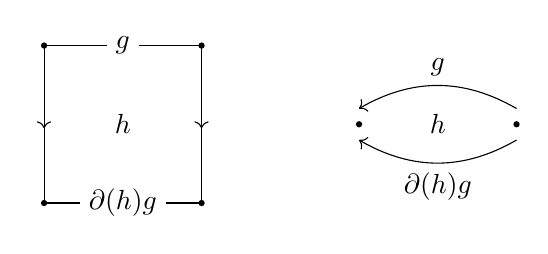
\begin{tikzpicture}[scale=2]
    \begin{scope}[xshift=0.0cm]
      \draw (0,0) to node[sloped] {\tikz{\draw[->](0,0)--(0.1,0);}} (0,-1);
      \draw (1,0) to node[sloped] {\tikz{\draw[->](0,0)--(0.1,0);}} (1,-1);
      \draw (0,0) to node[sloped] {\tikz{\draw[->](0,0)--(0.1,0);}} (1,0);
      \draw (0,-1) to node  {\tikz{\draw[-](0,0)--(0.1,0);}} (1,-1);
      \node at (1/2,-1/2) {$h$};
      \draw (0,0) to node [fill=white] {$g$} (1,0);
      \draw (0,-1) to node [fill=white] {$\del(h)g$} (1,-1);
      \fill[black] (0,0) circle[radius=0.02];
      \fill[black] (1,0) circle[radius=0.02];
      \fill[black] (0,-1) circle[radius=0.02];
      \fill[black] (1,-1) circle[radius=0.02];
    \end{scope}
    \begin{scope}[xshift=2.0cm, yshift=-0.5cm]
      \fill[black] (0,0) circle[radius=0.02];
      \fill[black] (1,0) circle[radius=0.02];
      \draw[<-] (0,0.1) to [out=30,in=150] node[midway] (g) {} (1,0.1)   ;
	      \node[above] at (g) {$g$};
	\draw[<-] (0,-0.1) to [out=-30,in=-150] node[midway] (g') {} (1,-0.1)   ;
	      \node[below] at (g') {$\del(h) g$};
	      \node at ($(g)!0.5!(g')$) {$h$};
    \end{scope}
  \end{tikzpicture}
\end{center}
\caption{Two types of $H$}
\label{d:2-mor}
\end{figure}

In this section, it is convenient to work with the cube-type representation; hence, we mainly use the cube-type diagrams.
The lattice-type diagrams are helpful for understanding the color conditions.
Occasionally, we present both cube-type and lattice-type diagrams for comparison, but in most cases we only use the cube-type in this section.
 
From now on, we denote the unit element $e_g$ of $G$ without a label, as shown in Figure~\ref{d:1-mor_e}.
\begin{figure}
 \begin{center}
  \begin{tikzpicture}[scale=2]
    \begin{scope}[xshift=0.0cm]
      %\draw (0,0) to node[sloped] {\tikz{\draw[->](0,0)--(0.1,0);}} (0,-1);
      %\draw (1,0) to node[sloped] {\tikz{\draw[->](0,0)--(0.1,0);}} (1,-1);
      \draw (0,0) to node[sloped] {\tikz{\draw[-](0,0)--(0.1,0);}} (1,0);
      %\draw (0,-1) to node  {\tikz{\draw[-](0,0)--(0.1,0);}} (1,-1);
      %\node at (1/2,-1/2) {$h_2$};
      \fill[black] (0,0) circle[radius=0.02];
      \fill[black] (1,0) circle[radius=0.02];
    \end{scope}
    \begin{scope}[xshift=1.5cm]
      %\draw (0,0) to node[sloped] {\tikz{\draw[->](0,0)--(0.1,0);}} (0,-1);
      %\draw (1,0) to node[sloped] {\tikz{\draw[->](0,0)--(0.1,0);}} (1,-1);
      \draw (0,0) to node [fill=white] {$e_g$} (1,0);
      %\draw (0,-1) to node {\tikz{\draw[-](0,0)--(0.1,0);}} (1,-1);
      \fill[black] (0,0) circle[radius=0.02];
      \fill[black] (1,0) circle[radius=0.02];
      %\node at (1/2,-1/2) {$h_1$};
    \end{scope}
    \node at (1.25, 0) {$\coloneqq$};
  \end{tikzpicture}
\end{center}
\caption{Unit element of $G$}
\label{d:1-mor_e}
\end{figure}

If the top edge of a square is determined, we can compute the bottom edge accordingly, so we may omit writing the label for the bottom edge.
For $h_1, h_2 \in H$, the product $h_2\#_2 h_1 \coloneqq h_2\cdot h_1$ is represented in Figure~\ref{d:2-mor_vertical}.
\begin{figure}
\begin{center}
  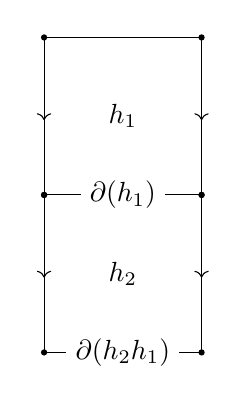
\begin{tikzpicture}[scale=2]
    \begin{scope}[xshift=0.0cm]
      \draw (0,0) to node[sloped] {\tikz{\draw[->](0,0)--(0.1,0);}} (0,-1);
      \draw (1,0) to node[sloped] {\tikz{\draw[->](0,0)--(0.1,0);}} (1,-1);
      \draw (0,0) to node[sloped] {\tikz{\draw[-](0,0)--(0.1,0);}} (1,0);
      \draw (0,-1) to node  {\tikz{\draw[-](0,0)--(0.1,0);}} (1,-1);
      \node at (1/2,-1/2) {$h_1$};
      \fill[black] (0,0) circle[radius=0.02];
      \fill[black] (1,0) circle[radius=0.02];
      \fill[black] (0,-1) circle[radius=0.02];
      \fill[black] (1,-1) circle[radius=0.02];
    \end{scope}
    \begin{scope}[yshift=-1.0cm]
      \draw (0,0) to node[sloped] {\tikz{\draw[->](0,0)--(0.1,0);}} (0,-1);
      \draw (1,0) to node[sloped] {\tikz{\draw[->](0,0)--(0.1,0);}} (1,-1);
      \draw (0,0) to node [fill=white] {$\del(h_1)$} (1,0);
      \draw (0,-1) to node [fill=white] {$\del(h_2 h_1)$} (1,-1);
      \node at (1/2,-1/2) {$h_2$};
      \fill[black] (0,0) circle[radius=0.02];
      \fill[black] (1,0) circle[radius=0.02];
      \fill[black] (0,-1) circle[radius=0.02];
      \fill[black] (1,-1) circle[radius=0.02];
    \end{scope}
  \end{tikzpicture}
\end{center}
\caption{Vertical compositon of $H$}
\label{d:2-mor_vertical}
\end{figure}

This product $h_2\#_2 h_1$ is called the {\bf vertical composion} in $H$ which is widely used in higher categories such as 2-categories and Gray categories. 
For each $g \in G$, we denote by ${\rm id}_g \in H$ an element satisfying ${\rm id}_g (g) = g$. Although ${\rm id}_g$ is not uniqe, the unit element of $H$ is always of this form. We depict ${\rm id}_g \in H$ in Figure~\ref{d:2-mor_unit}.
\begin{figure}
\begin{center}
  \begin{tikzpicture}[scale=2]
    \begin{scope}[xshift=0.0cm]
      \draw (0,0) to node[sloped] {\tikz{\draw[->](0,0)--(0.1,0);}} (0,-1);
      \draw (1,0) to node[sloped] {\tikz{\draw[->](0,0)--(0.1,0);}} (1,-1);
      \draw (0,0) to node[sloped] {\tikz{\draw[->](0,0)--(0.1,0);}} (1,0);
      \draw (0,-1) to node  {\tikz{\draw[-](0,0)--(0.1,0);}} (1,-1);
      \node at (1/2,-1/2) {$$};
      \draw (0,0) to node [fill=white] {$g$} (1,0);
      \draw (0,-1) to node [fill=white] {$g$} (1,-1);
      \fill[black] (0,0) circle[radius=0.02];
      \fill[black] (1,0) circle[radius=0.02];
      \fill[black] (0,-1) circle[radius=0.02];
      \fill[black] (1,-1) circle[radius=0.02];
    \end{scope}
     \begin{scope}[xshift=2.0cm]
      \draw (0,0) to node[sloped] {\tikz{\draw[->](0,0)--(0.1,0);}} (0,-1);
      \draw (1,0) to node[sloped] {\tikz{\draw[->](0,0)--(0.1,0);}} (1,-1);
      \draw (0,0) to node[sloped] {\tikz{\draw[->](0,0)--(0.1,0);}} (1,0);
      \draw (0,-1) to node  {\tikz{\draw[-](0,0)--(0.1,0);}} (1,-1);
      \node at (1/2,-1/2) {${\rm id}_g$};
      \draw (0,0) to node [fill=white] {$g$} (1,0);
      \draw (0,-1) to node [fill=white] {$g$} (1,-1);
      \fill[black] (0,0) circle[radius=0.02];
      \fill[black] (1,0) circle[radius=0.02];
      \fill[black] (0,-1) circle[radius=0.02];
      \fill[black] (1,-1) circle[radius=0.02];
    \end{scope}
        \node at (1.5,-1/2) {$\coloneqq$};
  \end{tikzpicture}
\end{center}
\caption{Unit element of $H$}
\label{d:2-mor_unit}
\end{figure}

We will omit the label for ${\rm id}_g \in H$ in the following diagrams.

For $g_1, g_2 \in G$ and $h_1, {\rm id}_{g_2} \in H$, and assume that $h_1(g_1) = g'_1$. Then there exists a {\bf horizontal compositon} ${\rm id}_{g_2} \#_1 h_1 (g_2\#_1 g_1 ) = g_2\#_1 g'_1$, which is illustrated in Figure~\ref{d:2-mor_L_hori}. 

\begin{figure}
\begin{center}
  \begin{tikzpicture}[scale=2]
    \begin{scope}[xshift=0.0cm]
      \draw (0,0) to node[sloped] {\tikz{\draw[->](0,0)--(0.1,0);}} (0,-1);
      \draw (1,0) to node[sloped] {\tikz{\draw[->](0,0)--(0.1,0);}} (1,-1);
      \draw (0,0) to node[sloped] {\tikz{\draw[->](0,0)--(0.1,0);}} (1,0);
      \draw (0,-1) to node  {\tikz{\draw[-](0,0)--(0.1,0);}} (1,-1);
      \node at (1/2,-1/2) {$$};
      \draw (0,0) to node [fill=white] {$g_2$} (1,0);
      \draw (0,-1) to node [fill=white] {$g_2$} (1,-1);
      \fill[black] (0,0) circle[radius=0.02];
      \fill[black] (1,0) circle[radius=0.02];
      \fill[black] (0,-1) circle[radius=0.02];
      \fill[black] (1,-1) circle[radius=0.02];
    \end{scope}
    \begin{scope}[xshift=1.0cm]
      \draw (0,0) to node[sloped] {\tikz{\draw[->](0,0)--(0.1,0);}} (0,-1);
      \draw (1,0) to node[sloped] {\tikz{\draw[->](0,0)--(0.1,0);}} (1,-1);
      \draw (0,0) to node[sloped] {\tikz{\draw[->](0,0)--(0.1,0);}} (1,0);
      \draw (0,-1) to node  {\tikz{\draw[-](0,0)--(0.1,0);}} (1,-1);
      \node at (1/2,-1/2) {$h_1$};
      \draw (0,0) to node [fill=white] {$g_1$} (1,0);
      \draw (0,-1) to node [fill=white] {$g_1'$} (1,-1);
      \fill[black] (0,0) circle[radius=0.02];
      \fill[black] (1,0) circle[radius=0.02];
      \fill[black] (0,-1) circle[radius=0.02];
      \fill[black] (1,-1) circle[radius=0.02];
    \end{scope}
     \begin{scope}[xshift=3.0cm, yshift=-0.5cm]
      \fill[black] (0,0) circle[radius=0.02];
      \fill[black] (1,0) circle[radius=0.02];
       \fill[black] (2,0) circle[radius=0.02];
      \draw[<-] (1.1,0.1) to [out=30,in=150] node[midway] (g1) {} (1.9,0.1)   ;
	      \node[above] at (g1) {$g_1$};
	\draw[<-] (1.1,-0.1) to [out=-30,in=-150] node[midway] (g1') {} (1.9,-0.1)   ;
	      \node[below] at (g1') {$g_1'$};
	      \node at ($(g1)!0.5!(g1')$) {$h_1$};
	\draw[<-] (0.1,0) to [out=0,in=0] node[midway] (g2) {} (0.8,0);
	 \node[above] at (0.5,0) {$g_2$};
    \end{scope}
  \end{tikzpicture}
\end{center}
\caption{Horizontal compositon of $H$}
\label{d:2-mor_L_hori}
\end{figure}

We can reinterpret this horizontal composition ${\rm id}_{g_2} \#_1 h_1$ in categorical language as $\act{g_2}h_1$ when written in the language of groups, according to the following formula:
\begin{align*}
\act{g_2}h_1 (g_2\cdot g_1) &= \partial(\act{g_2}h_1 )g_2\cdot g_1\\
&= g_2 \cdot \partial(h_1) \cdot g_2^{-1} \cdot g_2 \cdot g_1\\
&= g_2 \cdot \partial(h_1) \cdot g_1\\
&= g_2 \cdot h_1(g_1)\\
&= g_2 \cdot g'_1 \\
&= {\rm id}_{g_2} \#_1 h_1 (g_2\#_1 g_1 ).
\end{align*}

For $g_1, g_2 \in G$ and $ {\rm id}_{g_1}, h_2\in H$, assume that $h_2(g_2) = g'_2$. There is a switched version of the horizontal composition:  $h_2 \#_1 {\rm id}_{g_1}  (g_2\#_1 g_1 ) = g'_2\#_1 g_1$. We represent $h_2 \#_1 {\rm id}_{g_1}$ in Figure~\ref{d:2-mor_R_hori}.

\begin{figure}
\begin{center}
  \begin{tikzpicture}[scale=2]
    \begin{scope}[xshift=0.0cm]
      \draw (0,0) to node[sloped] {\tikz{\draw[->](0,0)--(0.1,0);}} (0,-1);
      \draw (1,0) to node[sloped] {\tikz{\draw[->](0,0)--(0.1,0);}} (1,-1);
      \draw (0,0) to node[sloped] {\tikz{\draw[->](0,0)--(0.1,0);}} (1,0);
      \draw (0,-1) to node  {\tikz{\draw[-](0,0)--(0.1,0);}} (1,-1);
      \node at (1/2,-1/2) {$h_2$};
      \draw (0,0) to node [fill=white] {$g_2$} (1,0);
      \draw (0,-1) to node [fill=white] {$g_2'$} (1,-1);
      \fill[black] (0,0) circle[radius=0.02];
      \fill[black] (1,0) circle[radius=0.02];
      \fill[black] (0,-1) circle[radius=0.02];
      \fill[black] (1,-1) circle[radius=0.02];
    \end{scope}
    \begin{scope}[xshift=1.0cm]
      \draw (0,0) to node[sloped] {\tikz{\draw[->](0,0)--(0.1,0);}} (0,-1);
      \draw (1,0) to node[sloped] {\tikz{\draw[->](0,0)--(0.1,0);}} (1,-1);
      \draw (0,0) to node[sloped] {\tikz{\draw[->](0,0)--(0.1,0);}} (1,0);
      \draw (0,-1) to node  {\tikz{\draw[-](0,0)--(0.1,0);}} (1,-1);
      \node at (1/2,-1/2) {$$};
      \draw (0,0) to node [fill=white] {$g_1$} (1,0);
      \draw (0,-1) to node [fill=white] {$g_1$} (1,-1);
      \fill[black] (0,0) circle[radius=0.02];
      \fill[black] (1,0) circle[radius=0.02];
      \fill[black] (0,-1) circle[radius=0.02];
      \fill[black] (1,-1) circle[radius=0.02];
    \end{scope}
    \begin{scope}[xshift=3.0cm, yshift=-0.5cm]
      \fill[black] (0,0) circle[radius=0.02];
      \fill[black] (1,0) circle[radius=0.02];
       \fill[black] (2,0) circle[radius=0.02];
      \draw[<-] (0.1,0.1) to [out=30,in=150] node[midway] (g1) {} (0.9,0.1)   ;
	      \node[above] at (g1) {$g_2$};
	\draw[<-] (0.1,-0.1) to [out=-30,in=-150] node[midway] (g1') {} (0.9,-0.1)   ;
	      \node[below] at (g1') {$g_2'$};
	      \node at ($(g1)!0.5!(g1')$) {$h_2$};
	\draw[<-] (1.1,0) to [out=0,in=0] node[midway] (g2) {} (1.8,0);
	 \node[above] at (1.5,0) {$g_1$};
    \end{scope}
  \end{tikzpicture}
\end{center}
\caption{Horizontal compositon of $H$}
\label{d:2-mor_R_hori}
\end{figure}

By the same discussion as for ${\rm id}_{g_2} \#_1 h_1$, the composition $h_2 \#_1 {\rm id}_{g_1}$ can be reinterpreted as $h_2$, according to the following formula:
\begin{align*}
h_2 (g_2\cdot g_1) &=  \partial(h_2)g_2\cdot g_1\\
&=h_2(g_2)\cdot h_1 \\
&=g'_2 \cdot h_1 \\
&= h_2 \#_1 {\rm id}_{g_1}  (g_2\#_1 g_1 ) = g'_2\#_1 g_1
\end{align*}

For $h_1, h_2 \in H$ and $g_1, g_2 \in G$, assume that $h_1(g_1) = g'_1$ and $h_2(g_2) = g'_2$. We would like to define the horizontal composition $h_2\#_1 h_1 (g_2\#_1 g_1 ) = g'_2\#_1 g'_1$ as illustrated in Figure~\ref{d:not_well_hor}, but this composition is not well-defined.
\begin{figure}
\begin{center}
  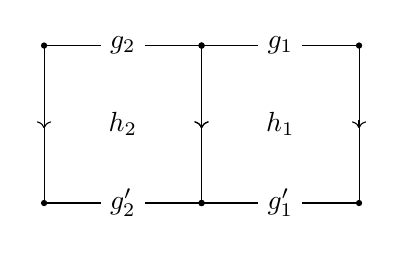
\begin{tikzpicture}[scale=2]
    \begin{scope}[xshift=0.0cm]
      \draw (0,0) to node[sloped] {\tikz{\draw[->](0,0)--(0.1,0);}} (0,-1);
      \draw (1,0) to node[sloped] {\tikz{\draw[->](0,0)--(0.1,0);}} (1,-1);
      \draw (0,0) to node[sloped] {\tikz{\draw[->](0,0)--(0.1,0);}} (1,0);
      \draw (0,-1) to node  {\tikz{\draw[-](0,0)--(0.1,0);}} (1,-1);
      \node at (1/2,-1/2) {$h_2$};
      \draw (0,0) to node [fill=white] {$g_2$} (1,0);
      \draw (0,-1) to node [fill=white] {$g_2'$} (1,-1);
      \fill[black] (0,0) circle[radius=0.02];
      \fill[black] (1,0) circle[radius=0.02];
      \fill[black] (0,-1) circle[radius=0.02];
      \fill[black] (1,-1) circle[radius=0.02];
    \end{scope}
    \begin{scope}[xshift=1.0cm]
      \draw (0,0) to node[sloped] {\tikz{\draw[->](0,0)--(0.1,0);}} (0,-1);
      \draw (1,0) to node[sloped] {\tikz{\draw[->](0,0)--(0.1,0);}} (1,-1);
      \draw (0,0) to node[sloped] {\tikz{\draw[->](0,0)--(0.1,0);}} (1,0);
      \draw (0,-1) to node  {\tikz{\draw[-](0,0)--(0.1,0);}} (1,-1);
      \node at (1/2,-1/2) {$h_1$};
      \draw (0,0) to node [fill=white] {$g_1$} (1,0);
      \draw (0,-1) to node [fill=white] {$g_1'$} (1,-1);
      \fill[black] (0,0) circle[radius=0.02];
      \fill[black] (1,0) circle[radius=0.02];
      \fill[black] (0,-1) circle[radius=0.02];
      \fill[black] (1,-1) circle[radius=0.02];
    \end{scope}
  \end{tikzpicture}
\end{center}
\caption{Image of $h_2\#_1 h_1$}
\label{d:not_well_hor}
\end{figure}

\begin{figure}
\begin{center}
  \begin{tikzpicture}[scale=2]
    \begin{scope}[xshift=0.0cm]
      \draw (0,0) to node[sloped] {\tikz{\draw[->](0,0)--(0.1,0);}} (0,-1);
      \draw (1,0) to node[sloped] {\tikz{\draw[->](0,0)--(0.1,0);}} (1,-1);
      \draw (0,0) to node[sloped] {\tikz{\draw[->](0,0)--(0.1,0);}} (1,0);
      \draw (0,-1) to node  {\tikz{\draw[-](0,0)--(0.1,0);}} (1,-1);
      \node at (1/2,-1/2) {$h_2$};
      \draw (0,0) to node [fill=white] {$g_2$} (1,0);
      \draw (0,-1) to node [fill=white] {$g_2'$} (1,-1);
      \fill[black] (0,0) circle[radius=0.02];
      \fill[black] (1,0) circle[radius=0.02];
      \fill[black] (0,-1) circle[radius=0.02];
      \fill[black] (1,-1) circle[radius=0.02];
    \end{scope}
    \begin{scope}[xshift=1.0cm]
      \draw (0,0) to node[sloped] {\tikz{\draw[->](0,0)--(0.1,0);}} (0,-1);
      \draw (1,0) to node[sloped] {\tikz{\draw[->](0,0)--(0.1,0);}} (1,-1);
      \draw (0,0) to node[sloped] {\tikz{\draw[->](0,0)--(0.1,0);}} (1,0);
      \draw (0,-1) to node  {\tikz{\draw[-](0,0)--(0.1,0);}} (1,-1);
      \node at (1/2,-1/2) {$$};
      \draw (0,0) to node [fill=white] {$g_1$} (1,0);
      \draw (0,-1) to node [fill=white] {$g_1$} (1,-1);
      \fill[black] (0,0) circle[radius=0.02];
      \fill[black] (1,0) circle[radius=0.02];
      \fill[black] (0,-1) circle[radius=0.02];
      \fill[black] (1,-1) circle[radius=0.02];
    \end{scope}
        \begin{scope}[xshift=0.0cm, yshift = -1.0cm]
      \draw (0,0) to node[sloped] {\tikz{\draw[->](0,0)--(0.1,0);}} (0,-1);
      \draw (1,0) to node[sloped] {\tikz{\draw[->](0,0)--(0.1,0);}} (1,-1);
      \draw (0,0) to node[sloped] {\tikz{\draw[->](0,0)--(0.1,0);}} (1,0);
      \draw (0,-1) to node  {\tikz{\draw[-](0,0)--(0.1,0);}} (1,-1);
      \node at (1/2,-1/2) {$$};
      \draw (0,0) to node [fill=white] {$g_2'$} (1,0);
      \draw (0,-1) to node [fill=white] {$g_2'$} (1,-1);
      \fill[black] (0,0) circle[radius=0.02];
      \fill[black] (1,0) circle[radius=0.02];
      \fill[black] (0,-1) circle[radius=0.02];
      \fill[black] (1,-1) circle[radius=0.02];
    \end{scope}
    \begin{scope}[xshift=1.0cm, yshift = -1.0cm]
      \draw (0,0) to node[sloped] {\tikz{\draw[->](0,0)--(0.1,0);}} (0,-1);
      \draw (1,0) to node[sloped] {\tikz{\draw[->](0,0)--(0.1,0);}} (1,-1);
      \draw (0,0) to node[sloped] {\tikz{\draw[->](0,0)--(0.1,0);}} (1,0);
      \draw (0,-1) to node  {\tikz{\draw[-](0,0)--(0.1,0);}} (1,-1);
      \node at (1/2,-1/2) {$h_1$};
      \draw (0,0) to node [fill=white] {$g_1$} (1,0);
      \draw (0,-1) to node [fill=white] {$g_1'$} (1,-1);
      \fill[black] (0,0) circle[radius=0.02];
      \fill[black] (1,0) circle[radius=0.02];
      \fill[black] (0,-1) circle[radius=0.02];
      \fill[black] (1,-1) circle[radius=0.02];
    \end{scope}
    
       \begin{scope}[xshift=3.0cm, yshift=-1.0cm]
 \fill[black] (0,0) circle[radius=0.02];
      \fill[black] (1,0) circle[radius=0.02];
      \fill[black] (2,0) circle[radius=0.02];
      \draw[<-] (0.1,0.1) to [out=30,in=150] node[midway] (g2) {} (0.9,0.1)   ;
	      \node[above] at (g2) {$g_2$};
	\draw[<-] (0.1,-0.1) to [out=-30,in=-150] node[midway] (g2') {} (0.9,-0.1)   ;
	      \node[below] at (g2') {$g_2'$};
	      \node at ($(g2)!0.5!(g2')$) {$(h_2,1)$};
	\draw[<-] (1.1,0.1) to [out=30,in=150] node[midway] (g1) {} (1.9,0.1)   ;
	      \node[above] at (g1) {$g_1$};
	\draw[<-] (1.1,-0.1) to [out=-30,in=-150] node[midway] (g1') {} (1.9,-0.1)   ;
	      \node[below] at (g1') {$g_1'$};
	      \node at ($(g1)!0.5!(g1')$) {$(h_1,2)$};      
    \end{scope}
    
  \end{tikzpicture}
\end{center}
\caption{Two types of $({\rm id}_{g'_2}\#_1 h_1) \#_2 (h_2\#_1 {\rm id}_{g_1})$}
\label{d:h1h2}
\end{figure}


The horizontal composition $h_2\#_1 h_1$ can be expressed in two equivalent ways: 
\[
({\rm id}_{g'_2}\#_1 h_1) \#_2 (h_2\#_1 {\rm id}_{g_1})
\]
and 
\[(h_2\#_1 {\rm id}_{g'_1}) \#_2 ({\rm id}_{g_2}\#_1 h_1).
\] 
These two compositions are illustrated in Figures~\ref{d:h1h2} and~\ref{d:h2h1}, respectively.

\begin{figure}[h]
\begin{center}
  \begin{tikzpicture}[scale=2]
    \begin{scope}[xshift=0.0cm]
      \draw (0,0) to node[sloped] {\tikz{\draw[->](0,0)--(0.1,0);}} (0,-1);
      \draw (1,0) to node[sloped] {\tikz{\draw[->](0,0)--(0.1,0);}} (1,-1);
      \draw (0,0) to node[sloped] {\tikz{\draw[->](0,0)--(0.1,0);}} (1,0);
      \draw (0,-1) to node  {\tikz{\draw[-](0,0)--(0.1,0);}} (1,-1);
      \node at (1/2,-1/2) {$$};
      \draw (0,0) to node [fill=white] {$g_2$} (1,0);
      \draw (0,-1) to node [fill=white] {$g_2$} (1,-1);
      \fill[black] (0,0) circle[radius=0.02];
      \fill[black] (1,0) circle[radius=0.02];
      \fill[black] (0,-1) circle[radius=0.02];
      \fill[black] (1,-1) circle[radius=0.02];
    \end{scope}
    \begin{scope}[xshift=1.0cm]
      \draw (0,0) to node[sloped] {\tikz{\draw[->](0,0)--(0.1,0);}} (0,-1);
      \draw (1,0) to node[sloped] {\tikz{\draw[->](0,0)--(0.1,0);}} (1,-1);
      \draw (0,0) to node[sloped] {\tikz{\draw[->](0,0)--(0.1,0);}} (1,0);
      \draw (0,-1) to node  {\tikz{\draw[-](0,0)--(0.1,0);}} (1,-1);
      \node at (1/2,-1/2) {$h_1$};
      \draw (0,0) to node [fill=white] {$g_1$} (1,0);
      \draw (0,-1) to node [fill=white] {$g_1'$} (1,-1);
      \fill[black] (0,0) circle[radius=0.02];
      \fill[black] (1,0) circle[radius=0.02];
      \fill[black] (0,-1) circle[radius=0.02];
      \fill[black] (1,-1) circle[radius=0.02];
    \end{scope}
        \begin{scope}[xshift=0.0cm, yshift = -1.0cm]
      \draw (0,0) to node[sloped] {\tikz{\draw[->](0,0)--(0.1,0);}} (0,-1);
      \draw (1,0) to node[sloped] {\tikz{\draw[->](0,0)--(0.1,0);}} (1,-1);
      \draw (0,0) to node[sloped] {\tikz{\draw[->](0,0)--(0.1,0);}} (1,0);
      \draw (0,-1) to node  {\tikz{\draw[-](0,0)--(0.1,0);}} (1,-1);
      \node at (1/2,-1/2) {$h_2$};
      \draw (0,0) to node [fill=white] {$g_2$} (1,0);
      \draw (0,-1) to node [fill=white] {$g_2'$} (1,-1);
      \fill[black] (0,0) circle[radius=0.02];
      \fill[black] (1,0) circle[radius=0.02];
      \fill[black] (0,-1) circle[radius=0.02];
      \fill[black] (1,-1) circle[radius=0.02];
    \end{scope}
    \begin{scope}[xshift=1.0cm, yshift = -1.0cm]
      \draw (0,0) to node[sloped] {\tikz{\draw[->](0,0)--(0.1,0);}} (0,-1);
      \draw (1,0) to node[sloped] {\tikz{\draw[->](0,0)--(0.1,0);}} (1,-1);
      \draw (0,0) to node[sloped] {\tikz{\draw[->](0,0)--(0.1,0);}} (1,0);
      \draw (0,-1) to node  {\tikz{\draw[-](0,0)--(0.1,0);}} (1,-1);
      \node at (1/2,-1/2) {$$};
      \draw (0,0) to node [fill=white] {$g_1'$} (1,0);
      \draw (0,-1) to node [fill=white] {$g_1'$} (1,-1);
      \fill[black] (0,0) circle[radius=0.02];
      \fill[black] (1,0) circle[radius=0.02];
      \fill[black] (0,-1) circle[radius=0.02];
      \fill[black] (1,-1) circle[radius=0.02];
    \end{scope}
    \begin{scope}[xshift=3.0cm, yshift=-1.0cm]
 \fill[black] (0,0) circle[radius=0.02];
      \fill[black] (1,0) circle[radius=0.02];
      \fill[black] (2,0) circle[radius=0.02];
      \draw[<-] (0.1,0.1) to [out=30,in=150] node[midway] (g2) {} (0.9,0.1)   ;
	      \node[above] at (g2) {$g_2$};
	\draw[<-] (0.1,-0.1) to [out=-30,in=-150] node[midway] (g2') {} (0.9,-0.1)   ;
	      \node[below] at (g2') {$g_2'$};
	      \node at ($(g2)!0.5!(g2')$) {$(h_2,2)$};
	\draw[<-] (1.1,0.1) to [out=30,in=150] node[midway] (g1) {} (1.9,0.1)   ;
	      \node[above] at (g1) {$g_1$};
	\draw[<-] (1.1,-0.1) to [out=-30,in=-150] node[midway] (g1') {} (1.9,-0.1)   ;
	      \node[below] at (g1') {$g_1'$};
	      \node at ($(g1)!0.5!(g1')$) {$(h_1,1)$};      
    \end{scope}
  \end{tikzpicture}
\end{center}
\caption{Two types of $(h_2\#_1 {\rm id}_{g'_1}) \#_2 ({\rm id}_{g_2}\#_1 h_1)$}
\label{d:h2h1}
\end{figure}

In the lattice-type representation, we must distinguish which element of $H$ acts first. To do this, we introduce an ordered pair, whose first component is the element of $H$, and whose second component is a natural number indicating the order in which the elements of $H$ are applied.

From the discussion above, we obtain 
\[
({\rm id}_{g'_2}\#_1 h_1) \#_2 (h_2\#_1 {\rm id}_{g_1}) \coloneqq \act{g'_2}h_1\cdot h_2 = \act{\partial(h_2)g_2}h_1\cdot h_2,
\]
and 
\[
(h_2\#_1 {\rm id}_{g'_1}) \#_2 ({\rm id}_{g_2}\#_1 h_1) \coloneqq h_2 \cdot \act{g_2}h_1.
\]
As in the case of $H$, each element of $L$ can be regarded as a map
\[
l : H \longrightarrow H, \qquad h \longmapsto \partial(l)\,h ,
\]
This correspondence is illustrated in Figure~\ref{d:l}.
\begin{figure}
\begin{center}
  \begin{tikzpicture}[scale=2]
    \begin{scope}[xshift=0.0cm]
      \draw (0,0) to node[sloped] {\tikz{\draw[->](0,0)--(0.1,0);}} (0,-1);
      \draw (1,0) to node[sloped] {\tikz{\draw[->](0,0)--(0.1,0);}} (1,-1);
      \draw (0,0) to node[sloped] {\tikz{\draw[-](0,0)--(0.1,0);}} (1,0);
      \draw (0,-1) to node  {\tikz{\draw[-](0,0)--(0.1,0);}} (1,-1);
      \node at (1/2,-1/2) {$h$};
      \draw (0,0) to node {\tikz{\draw[-](0,0)--(0.1,0);}} (1,0);
      \draw (0,-1) to node {\tikz{\draw[-](0,0)--(0.1,0);}} (1,-1);
      \fill[black] (0,0) circle[radius=0.02];
      \fill[black] (1,0) circle[radius=0.02];
      \fill[black] (0,-1) circle[radius=0.02];
      \fill[black] (1,-1) circle[radius=0.02];
      \draw[->] (1.1,-1/2) to (1.9,-1/2);
      \node at (1.5,-1/2) [above]{$l$};
    \end{scope}
    \begin{scope}[xshift=2.0cm]
      \draw (0,0) to node[sloped] {\tikz{\draw[->](0,0)--(0.1,0);}} (0,-1);
      \draw (1,0) to node[sloped] {\tikz{\draw[->](0,0)--(0.1,0);}} (1,-1);
      \draw (0,0) to node[sloped] {\tikz{\draw[-](0,0)--(0.1,0);}} (1,0);
      \draw (0,-1) to node  {\tikz{\draw[-](0,0)--(0.1,0);}} (1,-1);
      \node at (1/2,-1/2) {$\del(l)h$};
      \draw (0,0) to node {\tikz{\draw[-](0,0)--(0.1,0);}} (1,0);
      \draw (0,-1) to node {\tikz{\draw[-](0,0)--(0.1,0);}} (1,-1);
      \fill[black] (0,0) circle[radius=0.02];
      \fill[black] (1,0) circle[radius=0.02];
      \fill[black] (0,-1) circle[radius=0.02];
      \fill[black] (1,-1) circle[radius=0.02];
	\end{scope}
  \end{tikzpicture}
\end{center}
\caption{Diagram of $L$}
\label{d:l}
\end{figure}

We denote the vertical composition of $l_2,l_1 \in L$ as $l_2 \#_3 l_1$. In diagrams, the vertical composition $l_2 \#_3 l_1$ is represented in Figure~\ref{d:ver_of_l}.
\begin{figure}[!]
\begin{center}
  \begin{tikzpicture}[scale=2]
    \begin{scope}[xshift=0.0cm]
      \draw[->] (1.1,-1/2) to (2.4,-1/2);
      \node at (1.75,-1/2) [above]{$l_1$};
      \draw (0,0) to node[sloped] {\tikz{\draw[->](0,0)--(0.1,0);}} (0,-1);
      \draw (1,0) to node[sloped] {\tikz{\draw[->](0,0)--(0.1,0);}} (1,-1);
      \draw (0,0) to node[sloped] {\tikz{\draw[-](0,0)--(0.1,0);}} (1,0);
      \draw (0,-1) to node  {\tikz{\draw[-](0,0)--(0.1,0);}} (1,-1);
      \node at (1/2,-1/2) {$h$};
      \draw (0,0) to node {\tikz{\draw[-](0,0)--(0.1,0);}} (1,0);
      \draw (0,-1) to node {\tikz{\draw[-](0,0)--(0.1,0);}}(1,-1);
      \fill[black] (0,0) circle[radius=0.02];
      \fill[black] (1,0) circle[radius=0.02];
      \fill[black] (0,-1) circle[radius=0.02];
      \fill[black] (1,-1) circle[radius=0.02];   
	  \end{scope}
	  \begin{scope}[xshift=2.5cm]
      \draw[->] (1.1,-1/2) to (2.4,-1/2);
      \node at (1.75,-1/2) [above]{$l_2$};
      \draw (0,0) to node[sloped] {\tikz{\draw[->](0,0)--(0.1,0);}} (0,-1);
      \draw (1,0) to node[sloped] {\tikz{\draw[->](0,0)--(0.1,0);}} (1,-1);
      \draw (0,0) to node[sloped] {\tikz{\draw[-](0,0)--(0.1,0);}} (1,0);
      \draw (0,-1) to node  {\tikz{\draw[-](0,0)--(0.1,0);}} (1,-1);
      \node at (1/2,-1/2) {$\del(l_1)h$};
      \draw (0,0) to node {\tikz{\draw[-](0,0)--(0.1,0);}} (1,0);
      \draw (0,-1) to node {\tikz{\draw[-](0,0)--(0.1,0);}}(1,-1);
      \fill[black] (0,0) circle[radius=0.02];
      \fill[black] (1,0) circle[radius=0.02];
      \fill[black] (0,-1) circle[radius=0.02];
      \fill[black] (1,-1) circle[radius=0.02];   
	  \end{scope}
	    \begin{scope}[xshift=5.0cm]
      \draw (0,0) to node[sloped] {\tikz{\draw[->](0,0)--(0.1,0);}} (0,-1);
      \draw (1,0) to node[sloped] {\tikz{\draw[->](0,0)--(0.1,0);}} (1,-1);
      \draw (0,0) to node[sloped] {\tikz{\draw[-](0,0)--(0.1,0);}} (1,0);
      \draw (0,-1) to node  {\tikz{\draw[-](0,0)--(0.1,0);}} (1,-1);
      \node at (1/2,-1/2) {$\del(l_2 l_1)h$};
      \draw (0,0) to node {\tikz{\draw[-](0,0)--(0.1,0);}} (1,0);
      \draw (0,-1) to node {\tikz{\draw[-](0,0)--(0.1,0);}}(1,-1);
      \fill[black] (0,0) circle[radius=0.02];
      \fill[black] (1,0) circle[radius=0.02];
      \fill[black] (0,-1) circle[radius=0.02];
      \fill[black] (1,-1) circle[radius=0.02];  
	  \end{scope}
	  \node at (3,-1.2) { \rotatebox{90}{$=$}};
	  \begin{scope}[xshift=1.5cm ,yshift=-1.4cm]
      \draw (0,0) to node[sloped] {\tikz{\draw[->](0,0)--(0.1,0);}} (0,-1);
      \draw (1,0) to node[sloped] {\tikz{\draw[->](0,0)--(0.1,0);}} (1,-1);
      \draw (0,0) to node[sloped] {\tikz{\draw[-](0,0)--(0.1,0);}} (1,0);
      \draw (0,-1) to node  {\tikz{\draw[-](0,0)--(0.1,0);}} (1,-1);
      \node at (1/2,-1/2) {$h$};
      \draw (0,0) to node {\tikz{\draw[-](0,0)--(0.1,0);}} (1,0);
      \draw (0,-1) to node {\tikz{\draw[-](0,0)--(0.1,0);}} (1,-1);
      \fill[black] (0,0) circle[radius=0.02];
      \fill[black] (1,0) circle[radius=0.02];
      \fill[black] (0,-1) circle[radius=0.02];
      \fill[black] (1,-1) circle[radius=0.02];
      \draw[->] (1.1,-1/2) to (1.9,-1/2);
      \node at (1.5,-1/2) [above]{$l_2 \#_3 l_1$};
    \begin{scope}[xshift=2.0cm]
      \draw (0,0) to node[sloped] {\tikz{\draw[->](0,0)--(0.1,0);}} (0,-1);
      \draw (1,0) to node[sloped] {\tikz{\draw[->](0,0)--(0.1,0);}} (1,-1);
      \draw (0,0) to node[sloped] {\tikz{\draw[-](0,0)--(0.1,0);}} (1,0);
      \draw (0,-1) to node  {\tikz{\draw[-](0,0)--(0.1,0);}} (1,-1);
      \node at (1/2,-1/2) {$\del(l_2 l_1)h$};
      \draw (0,0) to node {\tikz{\draw[-](0,0)--(0.1,0);}} (1,0);
      \draw (0,-1) to node {\tikz{\draw[-](0,0)--(0.1,0);}} (1,-1);
      \fill[black] (0,0) circle[radius=0.02];
      \fill[black] (1,0) circle[radius=0.02];
      \fill[black] (0,-1) circle[radius=0.02];
      \fill[black] (1,-1) circle[radius=0.02];
	\end{scope}
	\end{scope}
  \end{tikzpicture}
\end{center}
\caption{Vertical compositon of $L$}
\label{d:ver_of_l}
\end{figure}



For each $g_1,g_1',g_2,g_2'\in G$, $h_1,h_1', h_2,h_2'\in H$, and $l_1,l_2 \in L$, such that
\begin{equation*}
    \begin{aligned}
h_1(g_1) &= g_1',\ h_1'(g_1) = g_1'\\
h_2(g_2) &= g_2',\ h_2'(g_2) = g_2'\\
l_1(h_1)&= h_1',\ l_2(h_2) = h_2' .
    \end{aligned}
\end{equation*}
the elements ${\rm id}_{{\rm id}_{g_2}}\#_1 l_1$, and $l_2 \#_1{\rm id}_{{\rm id}_{g_1}}$ can be determined  in a manner analogous to the case of $H$ , and can be represented 
in Figures~\ref{d:hor1_of_l_1} and~\ref{d:hor1_of_l_2}, respectively.
\begin{figure}
\begin{center}
  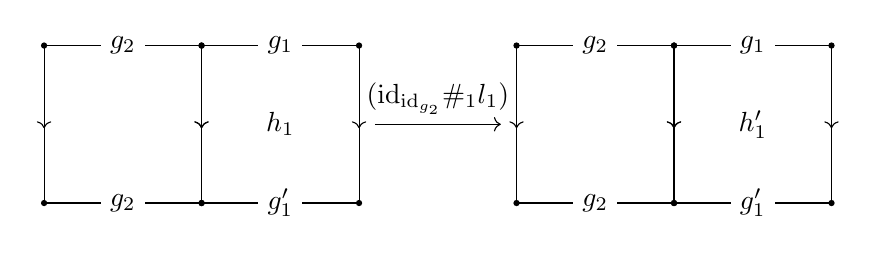
\begin{tikzpicture}[scale=2]
    \begin{scope}[xshift=0.0cm]
      \draw (0,0) to node[sloped] {\tikz{\draw[->](0,0)--(0.1,0);}} (0,-1);
      \draw (1,0) to node[sloped] {\tikz{\draw[->](0,0)--(0.1,0);}} (1,-1);
      \draw (0,0) to node[sloped] {\tikz{\draw[-](0,0)--(0.1,0);}} (1,0);
      \draw (0,-1) to node  {\tikz{\draw[-](0,0)--(0.1,0);}} (1,-1);
      \node at (1/2,-1/2) {$$};
      \draw (0,0) to node [fill=white] {$g_2$} (1,0);
      \draw (0,-1) to node[fill=white] {$g_2$} (1,-1);
      \fill[black] (0,0) circle[radius=0.02];
      \fill[black] (1,0) circle[radius=0.02];
      \fill[black] (0,-1) circle[radius=0.02];
      \fill[black] (1,-1) circle[radius=0.02];
       \begin{scope}[xshift=1.0cm]
      \draw (0,0) to node[sloped] {\tikz{\draw[->](0,0)--(0.1,0);}} (0,-1);
      \draw (1,0) to node[sloped] {\tikz{\draw[->](0,0)--(0.1,0);}} (1,-1);
      \draw (0,0) to node[sloped] {\tikz{\draw[-](0,0)--(0.1,0);}} (1,0);
      \draw (0,-1) to node  {\tikz{\draw[-](0,0)--(0.1,0);}} (1,-1);
      \node at (1/2,-1/2) {$h_1$};
      \draw (0,0) to node [fill=white] {$g_1$} (1,0);
      \draw (0,-1) to node [fill=white] {$g_1'$} (1,-1);
      \fill[black] (0,0) circle[radius=0.02];
      \fill[black] (1,0) circle[radius=0.02];
      \fill[black] (0,-1) circle[radius=0.02];
      \fill[black] (1,-1) circle[radius=0.02]; 
       \draw[->] (1.1,-1/2) to (1.9,-1/2);  
      \node at (1.5,-1/2) [above]{$({\rm id}_{{\rm id}_{g_2}}\#_1 l_1)$};
	\end{scope}
    \begin{scope}[xshift=3.0cm]
      \draw (0,0) to node[sloped] {\tikz{\draw[->](0,0)--(0.1,0);}} (0,-1);
      \draw (1,0) to node[sloped] {\tikz{\draw[->](0,0)--(0.1,0);}} (1,-1);
      \draw (0,0) to node[sloped] {\tikz{\draw[-](0,0)--(0.1,0);}} (1,0);
      \draw (0,-1) to node  {\tikz{\draw[-](0,0)--(0.1,0);}} (1,-1);
      \node at (1/2,-1/2) {$$};
      \draw (0,0) to node [fill=white] {$g_2$} (1,0);
      \draw (0,-1) to node [fill=white] {$g_2$}(1,-1);
      \fill[black] (0,0) circle[radius=0.02];
      \fill[black] (1,0) circle[radius=0.02];
      \fill[black] (0,-1) circle[radius=0.02];
      \fill[black] (1,-1) circle[radius=0.02];
	\end{scope}
	 \begin{scope}[xshift=4.0cm]
      \draw (0,0) to node[sloped] {\tikz{\draw[->](0,0)--(0.1,0);}} (0,-1);
      \draw (1,0) to node[sloped] {\tikz{\draw[->](0,0)--(0.1,0);}} (1,-1);
      \draw (0,0) to node[sloped] {\tikz{\draw[-](0,0)--(0.1,0);}} (1,0);
      \draw (0,-1) to node  {\tikz{\draw[-](0,0)--(0.1,0);}} (1,-1);
      \node at (1/2,-1/2) {$h_1'$};
      \draw (0,0) to node [fill=white] {$g_1$} (1,0);
      \draw (0,-1) to node [fill=white] {$g_1'$} (1,-1);
      \fill[black] (0,0) circle[radius=0.02];
      \fill[black] (1,0) circle[radius=0.02];
      \fill[black] (0,-1) circle[radius=0.02];
      \fill[black] (1,-1) circle[radius=0.02];
	\end{scope}
	 \end{scope}
  \end{tikzpicture}
\end{center}
\caption{Diagram of ${\rm id}_{{\rm id}_{g_2}}\#_1 l_1$}
\label{d:hor1_of_l_1}
\end{figure}
\begin{figure}
\begin{center}
  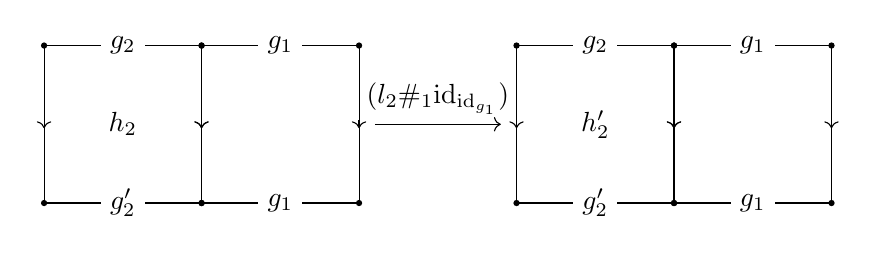
\begin{tikzpicture}[scale=2]
    \begin{scope}[xshift=0.0cm]
      \draw (0,0) to node[sloped] {\tikz{\draw[->](0,0)--(0.1,0);}} (0,-1);
      \draw (1,0) to node[sloped] {\tikz{\draw[->](0,0)--(0.1,0);}} (1,-1);
      \draw (0,0) to node[sloped] {\tikz{\draw[-](0,0)--(0.1,0);}} (1,0);
      \draw (0,-1) to node  {\tikz{\draw[-](0,0)--(0.1,0);}} (1,-1);
      \node at (1/2,-1/2) {$h_2$};
      \draw (0,0) to node [fill=white] {$g_2$} (1,0);
      \draw (0,-1) to node[fill=white] {$g_2'$} (1,-1);
      \fill[black] (0,0) circle[radius=0.02];
      \fill[black] (1,0) circle[radius=0.02];
      \fill[black] (0,-1) circle[radius=0.02];
      \fill[black] (1,-1) circle[radius=0.02];
       \begin{scope}[xshift=1.0cm]
      \draw (0,0) to node[sloped] {\tikz{\draw[->](0,0)--(0.1,0);}} (0,-1);
      \draw (1,0) to node[sloped] {\tikz{\draw[->](0,0)--(0.1,0);}} (1,-1);
      \draw (0,0) to node[sloped] {\tikz{\draw[-](0,0)--(0.1,0);}} (1,0);
      \draw (0,-1) to node  {\tikz{\draw[-](0,0)--(0.1,0);}} (1,-1);
      \node at (1/2,-1/2) {$$};
      \draw (0,0) to node [fill=white] {$g_1$} (1,0);
      \draw (0,-1) to node [fill=white] {$g_1$} (1,-1);
      \fill[black] (0,0) circle[radius=0.02];
      \fill[black] (1,0) circle[radius=0.02];
      \fill[black] (0,-1) circle[radius=0.02];
      \fill[black] (1,-1) circle[radius=0.02]; 
       \draw[->] (1.1,-1/2) to (1.9,-1/2);  
      \node at (1.5,-1/2) [above]{$(l_2 \#_1{\rm id}_{{\rm id}_{g_1}})$};
	\end{scope}
    \begin{scope}[xshift=3.0cm]
      \draw (0,0) to node[sloped] {\tikz{\draw[->](0,0)--(0.1,0);}} (0,-1);
      \draw (1,0) to node[sloped] {\tikz{\draw[->](0,0)--(0.1,0);}} (1,-1);
      \draw (0,0) to node[sloped] {\tikz{\draw[-](0,0)--(0.1,0);}} (1,0);
      \draw (0,-1) to node  {\tikz{\draw[-](0,0)--(0.1,0);}} (1,-1);
      \node at (1/2,-1/2) {$h_2'$};
      \draw (0,0) to node [fill=white] {$g_2$} (1,0);
      \draw (0,-1) to node [fill=white] {$g_2'$}(1,-1);
      \fill[black] (0,0) circle[radius=0.02];
      \fill[black] (1,0) circle[radius=0.02];
      \fill[black] (0,-1) circle[radius=0.02];
      \fill[black] (1,-1) circle[radius=0.02];
	\end{scope}
	 \begin{scope}[xshift=4.0cm]
      \draw (0,0) to node[sloped] {\tikz{\draw[->](0,0)--(0.1,0);}} (0,-1);
      \draw (1,0) to node[sloped] {\tikz{\draw[->](0,0)--(0.1,0);}} (1,-1);
      \draw (0,0) to node[sloped] {\tikz{\draw[-](0,0)--(0.1,0);}} (1,0);
      \draw (0,-1) to node  {\tikz{\draw[-](0,0)--(0.1,0);}} (1,-1);
      \node at (1/2,-1/2) {$$};
      \draw (0,0) to node [fill=white] {$g_1$} (1,0);
      \draw (0,-1) to node [fill=white] {$g_1$} (1,-1);
      \fill[black] (0,0) circle[radius=0.02];
      \fill[black] (1,0) circle[radius=0.02];
      \fill[black] (0,-1) circle[radius=0.02];
      \fill[black] (1,-1) circle[radius=0.02];
	\end{scope}
	 \end{scope}
  \end{tikzpicture}
\end{center}
\caption{Diagram of $l_2 \#_1{\rm id}_{{\rm id}_{g_1}}$}
\label{d:hor1_of_l_2}
\end{figure}
We can correspond ${\rm id}_{{\rm id}_{g_2}}\#_1 l_1$ as $\act{g_2}l_1$, and $l_2 \#_1{\rm id}_{{\rm id}_{g_1}}$ as $l_2$ in 3-crossed module.



 \begin{figure}[!]
 \begin{center}
  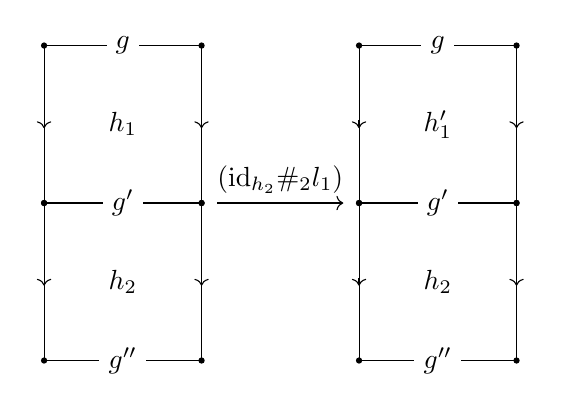
\begin{tikzpicture}[scale=2]
    \begin{scope}[xshift=0.0cm]
      \draw (0,0) to node[sloped] {\tikz{\draw[->](0,0)--(0.1,0);}} (0,-1);
      \draw (1,0) to node[sloped] {\tikz{\draw[->](0,0)--(0.1,0);}} (1,-1);
      \draw (0,0) to node[sloped] {\tikz{\draw[-](0,0)--(0.1,0);}} (1,0);
      \draw (0,-1) to node  {\tikz{\draw[-](0,0)--(0.1,0);}} (1,-1);
      \node at (1/2,-1/2) {$h_1$};
      \draw (0,0) to node [fill=white] {$g$} (1,0);
      \draw (0,-1) to node[fill=white] {$g'$} (1,-1);
      \fill[black] (0,0) circle[radius=0.02];
      \fill[black] (1,0) circle[radius=0.02];
      \fill[black] (0,-1) circle[radius=0.02];
      \fill[black] (1,-1) circle[radius=0.02];
       \draw[->] (1.1,-1) to (1.9,-1);  
      \node at (1.5,-1) [above]{$({\rm id}_{h_2}\#_2 l_1)$};
       \begin{scope}[yshift=-1.0cm]
      \draw (0,0) to node[sloped] {\tikz{\draw[->](0,0)--(0.1,0);}} (0,-1);
      \draw (1,0) to node[sloped] {\tikz{\draw[->](0,0)--(0.1,0);}} (1,-1);
      \draw (0,0) to node[sloped] {\tikz{\draw[-](0,0)--(0.1,0);}} (1,0);
      \draw (0,-1) to node  {\tikz{\draw[-](0,0)--(0.1,0);}} (1,-1);
      \node at (1/2,-1/2) {$h_2$};
      \draw (0,0) to node [fill=white] {$g'$} (1,0);
      \draw (0,-1) to node [fill=white] {$g''$} (1,-1);
      \fill[black] (0,0) circle[radius=0.02];
      \fill[black] (1,0) circle[radius=0.02];
      \fill[black] (0,-1) circle[radius=0.02];
      \fill[black] (1,-1) circle[radius=0.02]; 
	\end{scope}
    \begin{scope}[xshift=2.0cm]
      \draw (0,0) to node[sloped] {\tikz{\draw[->](0,0)--(0.1,0);}} (0,-1);
      \draw (1,0) to node[sloped] {\tikz{\draw[->](0,0)--(0.1,0);}} (1,-1);
      \draw (0,0) to node[sloped] {\tikz{\draw[-](0,0)--(0.1,0);}} (1,0);
      \draw (0,-1) to node  {\tikz{\draw[-](0,0)--(0.1,0);}} (1,-1);
      \node at (1/2,-1/2) {$h_1'$};
      \draw (0,0) to node [fill=white] {$g$} (1,0);
      \draw (0,-1) to node [fill=white] {$g'$}(1,-1);
      \fill[black] (0,0) circle[radius=0.02];
      \fill[black] (1,0) circle[radius=0.02];
      \fill[black] (0,-1) circle[radius=0.02];
      \fill[black] (1,-1) circle[radius=0.02];
	\end{scope}
	 \begin{scope}[xshift=2.0cm,yshift=-1.0cm]
      \draw (0,0) to node[sloped] {\tikz{\draw[->](0,0)--(0.1,0);}} (0,-1);
      \draw (1,0) to node[sloped] {\tikz{\draw[->](0,0)--(0.1,0);}} (1,-1);
      \draw (0,0) to node[sloped] {\tikz{\draw[-](0,0)--(0.1,0);}} (1,0);
      \draw (0,-1) to node  {\tikz{\draw[-](0,0)--(0.1,0);}} (1,-1);
      \node at (1/2,-1/2) {$h_2$};
      \draw (0,0) to node [fill=white] {$g'$} (1,0);
      \draw (0,-1) to node [fill=white] {$g''$} (1,-1);
      \fill[black] (0,0) circle[radius=0.02];
      \fill[black] (1,0) circle[radius=0.02];
      \fill[black] (0,-1) circle[radius=0.02];
      \fill[black] (1,-1) circle[radius=0.02];
	\end{scope}
	 \end{scope}
  \end{tikzpicture}
\end{center}
\caption{Diagram of ${\rm id}_{h_2}\#_2 l_1$}
\label{d:hor2_of_l_1}
\end{figure}



For each $g, g', g'' \in G$, $h_1,h_2,h_1',h_2'\in H$, and $l_1, l_2\in L$, such that
\begin{equation*}
    \begin{aligned}
h_1(g) &= g',\ &h_1'(g) = g',\\
h_2(g') &= g'',\ &h_2'(g') = g'',\\
l_1(h_1)&= h_1', \text{ and } &l_2(h_2) = h_2' , 
    \end{aligned}
\end{equation*}
%
 ${\rm id}_{h_2}\#_2 l_1$ and $l_2 \#_2{\rm id}_{h_1}$ can be determind in similar manner of the case of $H$ and it can be write 
 in Figures~\ref{d:hor2_of_l_1} and~\ref{d:hor2_of_l_2}, respectively.
We can correspond ${\rm id}_{h_2}\#_2 l_1$ to $\act{h_2}l_1$, and $l_2 \#_2{\rm id}_{h_1}$ to $l_2$ in the context of a 3-crossed module.

\begin{figure}[h]
 \begin{center}
  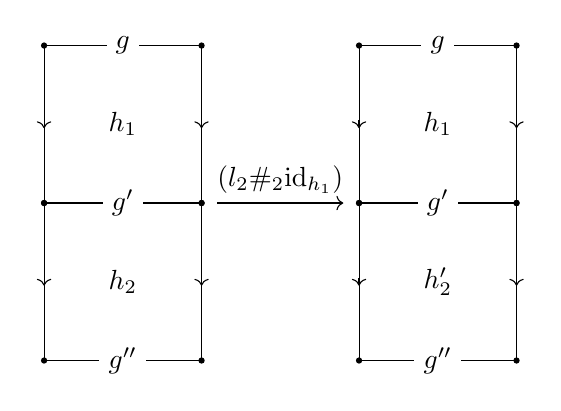
\begin{tikzpicture}[scale=2]
    \begin{scope}[xshift=0.0cm]
      \draw (0,0) to node[sloped] {\tikz{\draw[->](0,0)--(0.1,0);}} (0,-1);
      \draw (1,0) to node[sloped] {\tikz{\draw[->](0,0)--(0.1,0);}} (1,-1);
      \draw (0,0) to node[sloped] {\tikz{\draw[-](0,0)--(0.1,0);}} (1,0);
      \draw (0,-1) to node  {\tikz{\draw[-](0,0)--(0.1,0);}} (1,-1);
      \node at (1/2,-1/2) {$h_1$};
      \draw (0,0) to node [fill=white] {$g$} (1,0);
      \draw (0,-1) to node[fill=white] {$g'$} (1,-1);
      \fill[black] (0,0) circle[radius=0.02];
      \fill[black] (1,0) circle[radius=0.02];
      \fill[black] (0,-1) circle[radius=0.02];
      \fill[black] (1,-1) circle[radius=0.02];
       \draw[->] (1.1,-1) to (1.9,-1);  
      \node at (1.5,-1) [above]{$(l_2 \#_2{\rm id}_{h_1})$};
       \begin{scope}[yshift=-1.0cm]
      \draw (0,0) to node[sloped] {\tikz{\draw[->](0,0)--(0.1,0);}} (0,-1);
      \draw (1,0) to node[sloped] {\tikz{\draw[->](0,0)--(0.1,0);}} (1,-1);
      \draw (0,0) to node[sloped] {\tikz{\draw[-](0,0)--(0.1,0);}} (1,0);
      \draw (0,-1) to node  {\tikz{\draw[-](0,0)--(0.1,0);}} (1,-1);
      \node at (1/2,-1/2) {$h_2$};
      \draw (0,0) to node [fill=white] {$g'$} (1,0);
      \draw (0,-1) to node [fill=white] {$g''$} (1,-1);
      \fill[black] (0,0) circle[radius=0.02];
      \fill[black] (1,0) circle[radius=0.02];
      \fill[black] (0,-1) circle[radius=0.02];
      \fill[black] (1,-1) circle[radius=0.02]; 
	\end{scope}
    \begin{scope}[xshift=2.0cm]
      \draw (0,0) to node[sloped] {\tikz{\draw[->](0,0)--(0.1,0);}} (0,-1);
      \draw (1,0) to node[sloped] {\tikz{\draw[->](0,0)--(0.1,0);}} (1,-1);
      \draw (0,0) to node[sloped] {\tikz{\draw[-](0,0)--(0.1,0);}} (1,0);
      \draw (0,-1) to node  {\tikz{\draw[-](0,0)--(0.1,0);}} (1,-1);
      \node at (1/2,-1/2) {$h_1$};
      \draw (0,0) to node [fill=white] {$g$} (1,0);
      \draw (0,-1) to node [fill=white] {$g'$}(1,-1);
      \fill[black] (0,0) circle[radius=0.02];
      \fill[black] (1,0) circle[radius=0.02];
      \fill[black] (0,-1) circle[radius=0.02];
      \fill[black] (1,-1) circle[radius=0.02];
	\end{scope}
	 \begin{scope}[xshift=2.0cm,yshift=-1.0cm]
      \draw (0,0) to node[sloped] {\tikz{\draw[->](0,0)--(0.1,0);}} (0,-1);
      \draw (1,0) to node[sloped] {\tikz{\draw[->](0,0)--(0.1,0);}} (1,-1);
      \draw (0,0) to node[sloped] {\tikz{\draw[-](0,0)--(0.1,0);}} (1,0);
      \draw (0,-1) to node  {\tikz{\draw[-](0,0)--(0.1,0);}} (1,-1);
      \node at (1/2,-1/2) {$h_2'$};
      \draw (0,0) to node [fill=white] {$g'$} (1,0);
      \draw (0,-1) to node [fill=white] {$g''$} (1,-1);
      \fill[black] (0,0) circle[radius=0.02];
      \fill[black] (1,0) circle[radius=0.02];
      \fill[black] (0,-1) circle[radius=0.02];
      \fill[black] (1,-1) circle[radius=0.02];
	\end{scope}
	 \end{scope}
  \end{tikzpicture}
\end{center}
\caption{Diagram  of $l_2 \#_2{\rm id}_{h_1}$}
\label{d:hor2_of_l_2}
\end{figure}




By using the Peiffer lifting, we obtain a map 
$
({\rm id}_{g'_2}\#_1 h_1) \#_2 (h_2\#_1 {\rm id}_{g_1})
$ to $
(h_2\#_1 {\rm id}_{g'_1}) \#_2$ $ ({\rm id}_{g_2}\#_1 h_1).
$
\begin{equation}
  \begin{split} 
\label{pfmap}
\{h_2, \act{g_2}h_1 \}(\act{\partial(h_2)g_2}h_1\cdot h_2) &= \partial(\{h_2, \act{g_2}h_1 \})\cdot \act{\partial(h_2)g_2}h_1\cdot h_2\\
&=h_2\cdot \act{g_2}h_1\cdot h_2^{-1}\cdot \act{\partial(h_2)g_2}h_1^{-1}\cdot  \act{\partial(h_2)g_2} h_1\cdot h_2\\
&= h_2\cdot \act{g_2}h_1
 \end{split}
\end{equation}

Equation~(\ref{pfmap}) shows that $\{h_2, \act{g_2}h_1 \}$ defines a morphism from $({\rm id}_{g'_2}\#_1 h_1) \#_2 (h_2\#_1 {\rm id}_{g_1})$ to $(h_2\#_1 {\rm id}_{g'_1}) \#_2 ({\rm id}_{g_2}\#_1 h_1)$. If we assume $g_1=g_2=e_g$, equation~(\ref{pfmap}) can be written as $\{h_2, h_1 \}(\act{\partial(h_2)}h_1\cdot h_2) = h_2\cdot h_1$. The map $\{h_2, \act{g_2}h_1 \}$ is illustrated in Figure~\ref{d:PF_lift}.
\begin{figure}
\begin{center}
  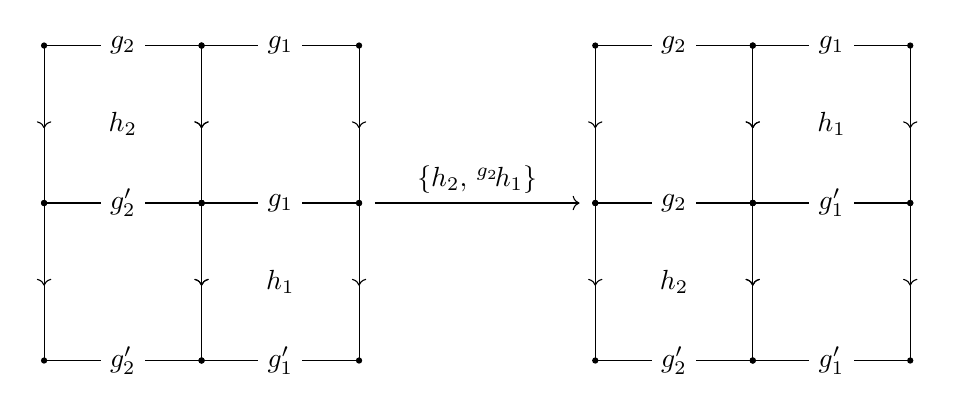
\begin{tikzpicture}[scale=2]
    \begin{scope}[xshift=0.0cm]
      \draw (0,0) to node[sloped] {\tikz{\draw[->](0,0)--(0.1,0);}} (0,-1);
      \draw (1,0) to node[sloped] {\tikz{\draw[->](0,0)--(0.1,0);}} (1,-1);
      \draw (0,0) to node[sloped] {\tikz{\draw[->](0,0)--(0.1,0);}} (1,0);
      \draw (0,-1) to node  {\tikz{\draw[-](0,0)--(0.1,0);}} (1,-1);
      \node at (1/2,-1/2) {$h_2$};
      \draw (0,0) to node [fill=white] {$g_2$} (1,0);
      \draw (0,-1) to node [fill=white] {$g_2'$} (1,-1);
      \fill[black] (0,0) circle[radius=0.02];
      \fill[black] (1,0) circle[radius=0.02];
      \fill[black] (0,-1) circle[radius=0.02];
      \fill[black] (1,-1) circle[radius=0.02];
    \end{scope}
    \begin{scope}[xshift=1.0cm]
      \draw (0,0) to node[sloped] {\tikz{\draw[->](0,0)--(0.1,0);}} (0,-1);
      \draw (1,0) to node[sloped] {\tikz{\draw[->](0,0)--(0.1,0);}} (1,-1);
      \draw (0,0) to node[sloped] {\tikz{\draw[->](0,0)--(0.1,0);}} (1,0);
      \draw (0,-1) to node  {\tikz{\draw[-](0,0)--(0.1,0);}} (1,-1);
      \node at (1/2,-1/2) {$$};
      \draw (0,0) to node [fill=white] {$g_1$} (1,0);
      \draw (0,-1) to node [fill=white] {$g_1$} (1,-1);
      \fill[black] (0,0) circle[radius=0.02];
      \fill[black] (1,0) circle[radius=0.02];
      \fill[black] (0,-1) circle[radius=0.02];
      \fill[black] (1,-1) circle[radius=0.02];
    \end{scope}
        \begin{scope}[xshift=0.0cm, yshift = -1.0cm]
      \draw (0,0) to node[sloped] {\tikz{\draw[->](0,0)--(0.1,0);}} (0,-1);
      \draw (1,0) to node[sloped] {\tikz{\draw[->](0,0)--(0.1,0);}} (1,-1);
      \draw (0,0) to node[sloped] {\tikz{\draw[->](0,0)--(0.1,0);}} (1,0);
      \draw (0,-1) to node  {\tikz{\draw[-](0,0)--(0.1,0);}} (1,-1);
      \node at (1/2,-1/2) {$$};
      \draw (0,0) to node [fill=white] {$g_2'$} (1,0);
      \draw (0,-1) to node [fill=white] {$g_2'$} (1,-1);
      \fill[black] (0,0) circle[radius=0.02];
      \fill[black] (1,0) circle[radius=0.02];
      \fill[black] (0,-1) circle[radius=0.02];
      \fill[black] (1,-1) circle[radius=0.02];
    \end{scope}
    \begin{scope}[xshift=1.0cm, yshift = -1.0cm]
      \draw (0,0) to node[sloped] {\tikz{\draw[->](0,0)--(0.1,0);}} (0,-1);
      \draw (1,0) to node[sloped] {\tikz{\draw[->](0,0)--(0.1,0);}} (1,-1);
      \draw (0,0) to node[sloped] {\tikz{\draw[->](0,0)--(0.1,0);}} (1,0);
      \draw (0,-1) to node  {\tikz{\draw[-](0,0)--(0.1,0);}} (1,-1);
      \node at (1/2,-1/2) {$h_1$};
      \draw (0,0) to node [fill=white] {$g_1$} (1,0);
      \draw (0,-1) to node [fill=white] {$g_1'$} (1,-1);
      \fill[black] (0,0) circle[radius=0.02];
      \fill[black] (1,0) circle[radius=0.02];
      \fill[black] (0,-1) circle[radius=0.02];
      \fill[black] (1,-1) circle[radius=0.02];
    \end{scope}
       \draw[->] (2.1,-1) to (3.4,-1);
      \node at (2.75,-1) [above]{$\{h_2, \act{g_2}h_1 \}$};
    \begin{scope}[xshift=3.5cm]
      \draw (0,0) to node[sloped] {\tikz{\draw[->](0,0)--(0.1,0);}} (0,-1);
      \draw (1,0) to node[sloped] {\tikz{\draw[->](0,0)--(0.1,0);}} (1,-1);
      \draw (0,0) to node[sloped] {\tikz{\draw[->](0,0)--(0.1,0);}} (1,0);
      \draw (0,-1) to node  {\tikz{\draw[-](0,0)--(0.1,0);}} (1,-1);
      \node at (1/2,-1/2) {$$};
      \draw (0,0) to node [fill=white] {$g_2$} (1,0);
      \draw (0,-1) to node [fill=white] {$g_2$} (1,-1);
      \fill[black] (0,0) circle[radius=0.02];
      \fill[black] (1,0) circle[radius=0.02];
      \fill[black] (0,-1) circle[radius=0.02];
      \fill[black] (1,-1) circle[radius=0.02];
    \end{scope}
    \begin{scope}[xshift=4.5cm]
      \draw (0,0) to node[sloped] {\tikz{\draw[->](0,0)--(0.1,0);}} (0,-1);
      \draw (1,0) to node[sloped] {\tikz{\draw[->](0,0)--(0.1,0);}} (1,-1);
      \draw (0,0) to node[sloped] {\tikz{\draw[->](0,0)--(0.1,0);}} (1,0);
      \draw (0,-1) to node  {\tikz{\draw[-](0,0)--(0.1,0);}} (1,-1);
      \node at (1/2,-1/2) {$h_1$};
      \draw (0,0) to node [fill=white] {$g_1$} (1,0);
      \draw (0,-1) to node [fill=white] {$g_1'$} (1,-1);
      \fill[black] (0,0) circle[radius=0.02];
      \fill[black] (1,0) circle[radius=0.02];
      \fill[black] (0,-1) circle[radius=0.02];
      \fill[black] (1,-1) circle[radius=0.02];
    \end{scope}
        \begin{scope}[xshift=3.5cm, yshift = -1.0cm]
      \draw (0,0) to node[sloped] {\tikz{\draw[->](0,0)--(0.1,0);}} (0,-1);
      \draw (1,0) to node[sloped] {\tikz{\draw[->](0,0)--(0.1,0);}} (1,-1);
      \draw (0,0) to node[sloped] {\tikz{\draw[->](0,0)--(0.1,0);}} (1,0);
      \draw (0,-1) to node  {\tikz{\draw[-](0,0)--(0.1,0);}} (1,-1);
      \node at (1/2,-1/2) {$h_2$};
      \draw (0,0) to node [fill=white] {$g_2$} (1,0);
      \draw (0,-1) to node [fill=white] {$g_2'$} (1,-1);
      \fill[black] (0,0) circle[radius=0.02];
      \fill[black] (1,0) circle[radius=0.02];
      \fill[black] (0,-1) circle[radius=0.02];
      \fill[black] (1,-1) circle[radius=0.02];
    \end{scope}
    \begin{scope}[xshift=4.5cm, yshift = -1.0cm]
      \draw (0,0) to node[sloped] {\tikz{\draw[->](0,0)--(0.1,0);}} (0,-1);
      \draw (1,0) to node[sloped] {\tikz{\draw[->](0,0)--(0.1,0);}} (1,-1);
      \draw (0,0) to node[sloped] {\tikz{\draw[->](0,0)--(0.1,0);}} (1,0);
      \draw (0,-1) to node  {\tikz{\draw[-](0,0)--(0.1,0);}} (1,-1);
      \node at (1/2,-1/2) {$$};
      \draw (0,0) to node [fill=white] {$g_1'$} (1,0);
      \draw (0,-1) to node [fill=white] {$g_1'$} (1,-1);
      \fill[black] (0,0) circle[radius=0.02];
      \fill[black] (1,0) circle[radius=0.02];
      \fill[black] (0,-1) circle[radius=0.02];
      \fill[black] (1,-1) circle[radius=0.02];
    \end{scope}
  \end{tikzpicture}
\end{center}
\caption{Diagram  of Peiffer lifting}
\label{d:PF_lift}
\end{figure}

By referring to the diagram of the Peiffer lifting, we can understand  we can visually understand Properties~\ref{lpl} and ~\ref{rpl} of the 2-crossed module. Let $h_1, h_2, h_3 \in H$, and consider $h_3 \#_1 h_2 \# h_1 (e_g \#_1 e_g \#_1 e_g ) = \del(h_3) \#_1 \del(h_2) \#_1 \del(h_1)$.  Property~\ref{lpl} of the 2-crossed module can be represented in Figure~\ref{d:PF_lift_left}, and Property~\ref{rpl} can be represented in Figure~\ref{d:PF_lift_right}.
\begin{figure}
\begin{center}
  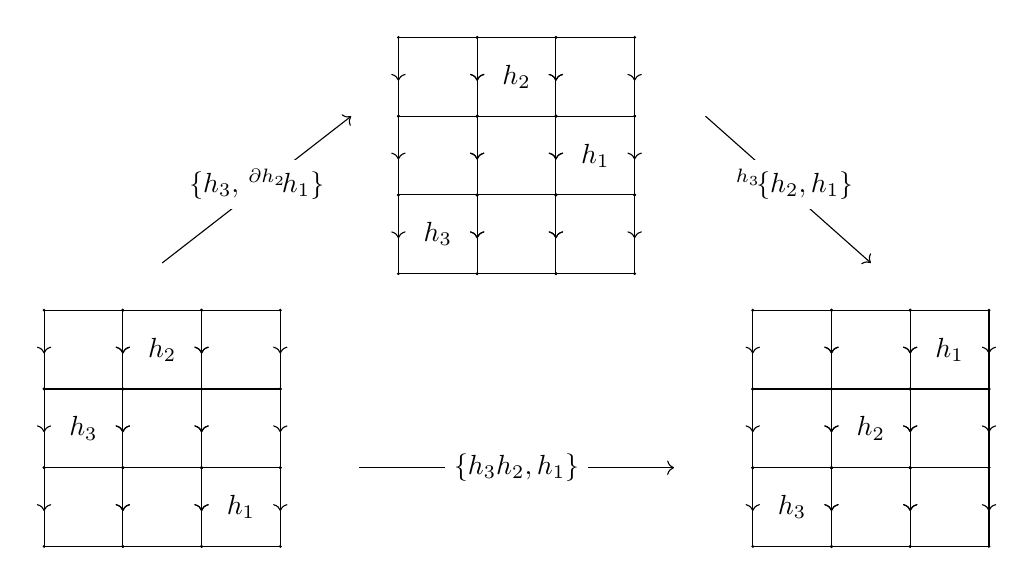
\begin{tikzpicture}[scale=1]
  	\begin{scope}[xshift=0.0cm]
	      \draw (0,0) to node[sloped] {\tikz{\draw[->](0,0)--(0.1,0);}} (0,-1);
	      \draw (1,0) to node[sloped] {\tikz{\draw[->](0,0)--(0.1,0);}} (1,-1);
	      \draw (0,0) to node[sloped] {\tikz{\draw[-](0,0)--(0.1,0);}} (1,0);
	      \draw (0,-1) to node  {\tikz{\draw[-](0,0)--(0.1,0);}} (1,-1);
	      \node at (1/2,-1/2) {$$};
	      \draw (0,0) to node {\tikz{\draw[-](0,0)--(0.1,0);}}(1,0);
	      \draw (0,-1) to node {\tikz{\draw[-](0,0)--(0.1,0);}} (1,-1);
	      \fill[black] (0,0) circle[radius=0.02];
	      \fill[black] (1,0) circle[radius=0.02];
	      \fill[black] (0,-1) circle[radius=0.02];
	      \fill[black] (1,-1) circle[radius=0.02];
	    \begin{scope}[xshift=1.0cm]
	      \draw (0,0) to node[sloped] {\tikz{\draw[->](0,0)--(0.1,0);}} (0,-1);
	      \draw (1,0) to node[sloped] {\tikz{\draw[->](0,0)--(0.1,0);}} (1,-1);
	      \draw (0,0) to node[sloped] {\tikz{\draw[-](0,0)--(0.1,0);}} (1,0);
	      \draw (0,-1) to node  {\tikz{\draw[-](0,0)--(0.1,0);}} (1,-1);
	      \node at (1/2,-1/2) {$h_2$};
	      \draw (0,0) to node {\tikz{\draw[-](0,0)--(0.1,0);}} (1,0);
	      \draw (0,-1) to node {\tikz{\draw[-](0,0)--(0.1,0);}} (1,-1);
	      \fill[black] (0,0) circle[radius=0.02];
	      \fill[black] (1,0) circle[radius=0.02];
	      \fill[black] (0,-1) circle[radius=0.02];
	      \fill[black] (1,-1) circle[radius=0.02];
	    \end{scope}
	    	 \begin{scope}[xshift=2.0cm]
	      \draw (0,0) to node[sloped] {\tikz{\draw[->](0,0)--(0.1,0);}} (0,-1);
	      \draw (1,0) to node[sloped] {\tikz{\draw[->](0,0)--(0.1,0);}} (1,-1);
	      \draw (0,0) to node[sloped] {\tikz{\draw[-](0,0)--(0.1,0);}} (1,0);
	      \draw (0,-1) to node  {\tikz{\draw[-](0,0)--(0.1,0);}} (1,-1);
	      \node at (1/2,-1/2) {$$};
	      \draw (0,0) to node {\tikz{\draw[-](0,0)--(0.1,0);}} (1,0);
	      \draw (0,-1) to node {\tikz{\draw[-](0,0)--(0.1,0);}} (1,-1);
	      \fill[black] (0,0) circle[radius=0.02];
	      \fill[black] (1,0) circle[radius=0.02];
	      \fill[black] (0,-1) circle[radius=0.02];
	      \fill[black] (1,-1) circle[radius=0.02];
	    \end{scope}
	        \begin{scope}[xshift=0.0cm, yshift = -1.0cm]
	      \draw (0,0) to node[sloped] {\tikz{\draw[->](0,0)--(0.1,0);}} (0,-1);
	      \draw (1,0) to node[sloped] {\tikz{\draw[->](0,0)--(0.1,0);}} (1,-1);
	      \draw (0,0) to node[sloped] {\tikz{\draw[-](0,0)--(0.1,0);}} (1,0);
	      \draw (0,-1) to node  {\tikz{\draw[-](0,0)--(0.1,0);}} (1,-1);
	      \node at (1/2,-1/2) {$h_3$};
	      \draw (0,0) to node {\tikz{\draw[-](0,0)--(0.1,0);}} (1,0);
	      \draw (0,-1) to node {\tikz{\draw[-](0,0)--(0.1,0);}} (1,-1);
	      \fill[black] (0,0) circle[radius=0.02];
	      \fill[black] (1,0) circle[radius=0.02];
	      \fill[black] (0,-1) circle[radius=0.02];
	      \fill[black] (1,-1) circle[radius=0.02];
	    \end{scope}
	    \begin{scope}[xshift=1.0cm, yshift = -1.0cm]
	      \draw (0,0) to node[sloped] {\tikz{\draw[->](0,0)--(0.1,0);}} (0,-1);
	      \draw (1,0) to node[sloped] {\tikz{\draw[->](0,0)--(0.1,0);}} (1,-1);
	      \draw (0,0) to node[sloped] {\tikz{\draw[-](0,0)--(0.1,0);}} (1,0);
	      \draw (0,-1) to node  {\tikz{\draw[-](0,0)--(0.1,0);}} (1,-1);
	      \node at (1/2,-1/2) {$$};
	      \draw (0,0) to node {\tikz{\draw[-](0,0)--(0.1,0);}} (1,0);
	      \draw (0,-1) to node {\tikz{\draw[-](0,0)--(0.1,0);}} (1,-1);
	      \fill[black] (0,0) circle[radius=0.02];
	      \fill[black] (1,0) circle[radius=0.02];
	      \fill[black] (0,-1) circle[radius=0.02];
	      \fill[black] (1,-1) circle[radius=0.02];
	    \end{scope}
	     \begin{scope}[xshift=2.0cm, yshift = -1.0cm]
	      \draw (0,0) to node[sloped] {\tikz{\draw[->](0,0)--(0.1,0);}} (0,-1);
	      \draw (1,0) to node[sloped] {\tikz{\draw[->](0,0)--(0.1,0);}} (1,-1);
	      \draw (0,0) to node[sloped] {\tikz{\draw[-](0,0)--(0.1,0);}} (1,0);
	      \draw (0,-1) to node  {\tikz{\draw[-](0,0)--(0.1,0);}} (1,-1);
	      \node at (1/2,-1/2) {$$};
	      \draw (0,0) to node {\tikz{\draw[-](0,0)--(0.1,0);}} (1,0);
	      \draw (0,-1) to node {\tikz{\draw[-](0,0)--(0.1,0);}} (1,-1);
	      \fill[black] (0,0) circle[radius=0.02];
	      \fill[black] (1,0) circle[radius=0.02];
	      \fill[black] (0,-1) circle[radius=0.02];
	      \fill[black] (1,-1) circle[radius=0.02];
	    \end{scope}
	     \begin{scope}[xshift=0.0cm, yshift = -2.0cm]
	      \draw (0,0) to node[sloped] {\tikz{\draw[->](0,0)--(0.1,0);}} (0,-1);
	      \draw (1,0) to node[sloped] {\tikz{\draw[->](0,0)--(0.1,0);}} (1,-1);
	      \draw (0,0) to node[sloped] {\tikz{\draw[-](0,0)--(0.1,0);}} (1,0);
	      \draw (0,-1) to node  {\tikz{\draw[-](0,0)--(0.1,0);}} (1,-1);
	      \node at (1/2,-1/2) {$$};
	      \draw (0,0) to node {\tikz{\draw[-](0,0)--(0.1,0);}} (1,0);
	      \draw (0,-1) to node {\tikz{\draw[-](0,0)--(0.1,0);}} (1,-1);
	      \fill[black] (0,0) circle[radius=0.02];
	      \fill[black] (1,0) circle[radius=0.02];
	      \fill[black] (0,-1) circle[radius=0.02];
	      \fill[black] (1,-1) circle[radius=0.02];
	    \end{scope}
	    \begin{scope}[xshift=1.0cm, yshift = -2.0cm]
	      \draw (0,0) to node[sloped] {\tikz{\draw[->](0,0)--(0.1,0);}} (0,-1);
	      \draw (1,0) to node[sloped] {\tikz{\draw[->](0,0)--(0.1,0);}} (1,-1);
	      \draw (0,0) to node[sloped] {\tikz{\draw[-](0,0)--(0.1,0);}} (1,0);
	      \draw (0,-1) to node  {\tikz{\draw[-](0,0)--(0.1,0);}} (1,-1);
	      \node at (1/2,-1/2) {$$};
	      \draw (0,0) to node {\tikz{\draw[-](0,0)--(0.1,0);}}(1,0);
	      \draw (0,-1) to node {\tikz{\draw[-](0,0)--(0.1,0);}} (1,-1);
	      \fill[black] (0,0) circle[radius=0.02];
	      \fill[black] (1,0) circle[radius=0.02];
	      \fill[black] (0,-1) circle[radius=0.02];
	      \fill[black] (1,-1) circle[radius=0.02];
	    \end{scope}
	     \begin{scope}[xshift=2.0cm, yshift = -2.0cm]
	      \draw (0,0) to node[sloped] {\tikz{\draw[->](0,0)--(0.1,0);}} (0,-1);
	      \draw (1,0) to node[sloped] {\tikz{\draw[->](0,0)--(0.1,0);}} (1,-1);
	      \draw (0,0) to node[sloped] {\tikz{\draw[-](0,0)--(0.1,0);}} (1,0);
	      \draw (0,-1) to node  {\tikz{\draw[-](0,0)--(0.1,0);}} (1,-1);
	      \node at (1/2,-1/2) {$h_1$};
	      \draw (0,0) to node {\tikz{\draw[-](0,0)--(0.1,0);}}(1,0);
	      \draw (0,-1) to node {\tikz{\draw[-](0,0)--(0.1,0);}} (1,-1);
	      \fill[black] (0,0) circle[radius=0.02];
	      \fill[black] (1,0) circle[radius=0.02];
	      \fill[black] (0,-1) circle[radius=0.02];
	      \fill[black] (1,-1) circle[radius=0.02];
	    \end{scope}
    \end{scope}
    \begin{scope}[xshift=4.5cm, yshift = 2*1.732cm]
	      \draw (0,0) to node[sloped] {\tikz{\draw[->](0,0)--(0.1,0);}} (0,-1);
	      \draw (1,0) to node[sloped] {\tikz{\draw[->](0,0)--(0.1,0);}} (1,-1);
	      \draw (0,0) to node[sloped] {\tikz{\draw[-](0,0)--(0.1,0);}} (1,0);
	      \draw (0,-1) to node  {\tikz{\draw[-](0,0)--(0.1,0);}} (1,-1);
	      \node at (1/2,-1/2) {$$};
	      \draw (0,0) to node {\tikz{\draw[-](0,0)--(0.1,0);}}(1,0);
	      \draw (0,-1) to node {\tikz{\draw[-](0,0)--(0.1,0);}} (1,-1);
	      \fill[black] (0,0) circle[radius=0.02];
	      \fill[black] (1,0) circle[radius=0.02];
	      \fill[black] (0,-1) circle[radius=0.02];
	      \fill[black] (1,-1) circle[radius=0.02];
	    \begin{scope}[xshift=1.0cm]
	      \draw (0,0) to node[sloped] {\tikz{\draw[->](0,0)--(0.1,0);}} (0,-1);
	      \draw (1,0) to node[sloped] {\tikz{\draw[->](0,0)--(0.1,0);}} (1,-1);
	      \draw (0,0) to node[sloped] {\tikz{\draw[-](0,0)--(0.1,0);}} (1,0);
	      \draw (0,-1) to node  {\tikz{\draw[-](0,0)--(0.1,0);}} (1,-1);
	      \node at (1/2,-1/2) {$h_2$};
	      \draw (0,0) to node {\tikz{\draw[-](0,0)--(0.1,0);}} (1,0);
	      \draw (0,-1) to node {\tikz{\draw[-](0,0)--(0.1,0);}} (1,-1);
	      \fill[black] (0,0) circle[radius=0.02];
	      \fill[black] (1,0) circle[radius=0.02];
	      \fill[black] (0,-1) circle[radius=0.02];
	      \fill[black] (1,-1) circle[radius=0.02];
	    \end{scope}
	    	 \begin{scope}[xshift=2.0cm]
	      \draw (0,0) to node[sloped] {\tikz{\draw[->](0,0)--(0.1,0);}} (0,-1);
	      \draw (1,0) to node[sloped] {\tikz{\draw[->](0,0)--(0.1,0);}} (1,-1);
	      \draw (0,0) to node[sloped] {\tikz{\draw[-](0,0)--(0.1,0);}} (1,0);
	      \draw (0,-1) to node  {\tikz{\draw[-](0,0)--(0.1,0);}} (1,-1);
	      \node at (1/2,-1/2) {$$};
	      \draw (0,0) to node {\tikz{\draw[-](0,0)--(0.1,0);}} (1,0);
	      \draw (0,-1) to node {\tikz{\draw[-](0,0)--(0.1,0);}} (1,-1);
	      \fill[black] (0,0) circle[radius=0.02];
	      \fill[black] (1,0) circle[radius=0.02];
	      \fill[black] (0,-1) circle[radius=0.02];
	      \fill[black] (1,-1) circle[radius=0.02];
	    \end{scope}
	        \begin{scope}[xshift=0.0cm, yshift = -1.0cm]
	      \draw (0,0) to node[sloped] {\tikz{\draw[->](0,0)--(0.1,0);}} (0,-1);
	      \draw (1,0) to node[sloped] {\tikz{\draw[->](0,0)--(0.1,0);}} (1,-1);
	      \draw (0,0) to node[sloped] {\tikz{\draw[-](0,0)--(0.1,0);}} (1,0);
	      \draw (0,-1) to node  {\tikz{\draw[-](0,0)--(0.1,0);}} (1,-1);
	      \node at (1/2,-1/2) {$$};
	      \draw (0,0) to node {\tikz{\draw[-](0,0)--(0.1,0);}} (1,0);
	      \draw (0,-1) to node {\tikz{\draw[-](0,0)--(0.1,0);}} (1,-1);
	      \fill[black] (0,0) circle[radius=0.02];
	      \fill[black] (1,0) circle[radius=0.02];
	      \fill[black] (0,-1) circle[radius=0.02];
	      \fill[black] (1,-1) circle[radius=0.02];
	    \end{scope}
	    \begin{scope}[xshift=1.0cm, yshift = -1.0cm]
	      \draw (0,0) to node[sloped] {\tikz{\draw[->](0,0)--(0.1,0);}} (0,-1);
	      \draw (1,0) to node[sloped] {\tikz{\draw[->](0,0)--(0.1,0);}} (1,-1);
	      \draw (0,0) to node[sloped] {\tikz{\draw[-](0,0)--(0.1,0);}} (1,0);
	      \draw (0,-1) to node  {\tikz{\draw[-](0,0)--(0.1,0);}} (1,-1);
	      \node at (1/2,-1/2) {$$};
	      \draw (0,0) to node {\tikz{\draw[-](0,0)--(0.1,0);}} (1,0);
	      \draw (0,-1) to node {\tikz{\draw[-](0,0)--(0.1,0);}} (1,-1);
	      \fill[black] (0,0) circle[radius=0.02];
	      \fill[black] (1,0) circle[radius=0.02];
	      \fill[black] (0,-1) circle[radius=0.02];
	      \fill[black] (1,-1) circle[radius=0.02];
	    \end{scope}
	     \begin{scope}[xshift=2.0cm, yshift = -1.0cm]
	      \draw (0,0) to node[sloped] {\tikz{\draw[->](0,0)--(0.1,0);}} (0,-1);
	      \draw (1,0) to node[sloped] {\tikz{\draw[->](0,0)--(0.1,0);}} (1,-1);
	      \draw (0,0) to node[sloped] {\tikz{\draw[-](0,0)--(0.1,0);}} (1,0);
	      \draw (0,-1) to node  {\tikz{\draw[-](0,0)--(0.1,0);}} (1,-1);
	      \node at (1/2,-1/2) {$h_1$};
	      \draw (0,0) to node {\tikz{\draw[-](0,0)--(0.1,0);}} (1,0);
	      \draw (0,-1) to node {\tikz{\draw[-](0,0)--(0.1,0);}} (1,-1);
	      \fill[black] (0,0) circle[radius=0.02];
	      \fill[black] (1,0) circle[radius=0.02];
	      \fill[black] (0,-1) circle[radius=0.02];
	      \fill[black] (1,-1) circle[radius=0.02];
	    \end{scope}
	     \begin{scope}[xshift=0.0cm, yshift = -2.0cm]
	      \draw (0,0) to node[sloped] {\tikz{\draw[->](0,0)--(0.1,0);}} (0,-1);
	      \draw (1,0) to node[sloped] {\tikz{\draw[->](0,0)--(0.1,0);}} (1,-1);
	      \draw (0,0) to node[sloped] {\tikz{\draw[-](0,0)--(0.1,0);}} (1,0);
	      \draw (0,-1) to node  {\tikz{\draw[-](0,0)--(0.1,0);}} (1,-1);
	      \node at (1/2,-1/2) {$h_3$};
	      \draw (0,0) to node {\tikz{\draw[-](0,0)--(0.1,0);}} (1,0);
	      \draw (0,-1) to node {\tikz{\draw[-](0,0)--(0.1,0);}} (1,-1);
	      \fill[black] (0,0) circle[radius=0.02];
	      \fill[black] (1,0) circle[radius=0.02];
	      \fill[black] (0,-1) circle[radius=0.02];
	      \fill[black] (1,-1) circle[radius=0.02];
	    \end{scope}
	    \begin{scope}[xshift=1.0cm, yshift = -2.0cm]
	      \draw (0,0) to node[sloped] {\tikz{\draw[->](0,0)--(0.1,0);}} (0,-1);
	      \draw (1,0) to node[sloped] {\tikz{\draw[->](0,0)--(0.1,0);}} (1,-1);
	      \draw (0,0) to node[sloped] {\tikz{\draw[-](0,0)--(0.1,0);}} (1,0);
	      \draw (0,-1) to node  {\tikz{\draw[-](0,0)--(0.1,0);}} (1,-1);
	      \node at (1/2,-1/2) {$$};
	      \draw (0,0) to node {\tikz{\draw[-](0,0)--(0.1,0);}}(1,0);
	      \draw (0,-1) to node {\tikz{\draw[-](0,0)--(0.1,0);}} (1,-1);
	      \fill[black] (0,0) circle[radius=0.02];
	      \fill[black] (1,0) circle[radius=0.02];
	      \fill[black] (0,-1) circle[radius=0.02];
	      \fill[black] (1,-1) circle[radius=0.02];
	    \end{scope}
	     \begin{scope}[xshift=2.0cm, yshift = -2.0cm]
	      \draw (0,0) to node[sloped] {\tikz{\draw[->](0,0)--(0.1,0);}} (0,-1);
	      \draw (1,0) to node[sloped] {\tikz{\draw[->](0,0)--(0.1,0);}} (1,-1);
	      \draw (0,0) to node[sloped] {\tikz{\draw[-](0,0)--(0.1,0);}} (1,0);
	      \draw (0,-1) to node  {\tikz{\draw[-](0,0)--(0.1,0);}} (1,-1);
	      \node at (1/2,-1/2) {$$};
	      \draw (0,0) to node {\tikz{\draw[-](0,0)--(0.1,0);}}(1,0);
	      \draw (0,-1) to node {\tikz{\draw[-](0,0)--(0.1,0);}} (1,-1);
	      \fill[black] (0,0) circle[radius=0.02];
	      \fill[black] (1,0) circle[radius=0.02];
	      \fill[black] (0,-1) circle[radius=0.02];
	      \fill[black] (1,-1) circle[radius=0.02];
	    \end{scope}
    \end{scope}
    \begin{scope}[xshift=9.0cm]
	      \draw (0,0) to node[sloped] {\tikz{\draw[->](0,0)--(0.1,0);}} (0,-1);
	      \draw (1,0) to node[sloped] {\tikz{\draw[->](0,0)--(0.1,0);}} (1,-1);
	      \draw (0,0) to node[sloped] {\tikz{\draw[-](0,0)--(0.1,0);}} (1,0);
	      \draw (0,-1) to node  {\tikz{\draw[-](0,0)--(0.1,0);}} (1,-1);
	      \node at (1/2,-1/2) {$$};
	      \draw (0,0) to node {\tikz{\draw[-](0,0)--(0.1,0);}}(1,0);
	      \draw (0,-1) to node {\tikz{\draw[-](0,0)--(0.1,0);}} (1,-1);
	      \fill[black] (0,0) circle[radius=0.02];
	      \fill[black] (1,0) circle[radius=0.02];
	      \fill[black] (0,-1) circle[radius=0.02];
	      \fill[black] (1,-1) circle[radius=0.02];
	    \begin{scope}[xshift=1.0cm]
	      \draw (0,0) to node[sloped] {\tikz{\draw[->](0,0)--(0.1,0);}} (0,-1);
	      \draw (1,0) to node[sloped] {\tikz{\draw[->](0,0)--(0.1,0);}} (1,-1);
	      \draw (0,0) to node[sloped] {\tikz{\draw[-](0,0)--(0.1,0);}} (1,0);
	      \draw (0,-1) to node  {\tikz{\draw[-](0,0)--(0.1,0);}} (1,-1);
	      \node at (1/2,-1/2) {$$};
	      \draw (0,0) to node {\tikz{\draw[-](0,0)--(0.1,0);}} (1,0);
	      \draw (0,-1) to node {\tikz{\draw[-](0,0)--(0.1,0);}} (1,-1);
	      \fill[black] (0,0) circle[radius=0.02];
	      \fill[black] (1,0) circle[radius=0.02];
	      \fill[black] (0,-1) circle[radius=0.02];
	      \fill[black] (1,-1) circle[radius=0.02];
	    \end{scope}
	    	 \begin{scope}[xshift=2.0cm]
	      \draw (0,0) to node[sloped] {\tikz{\draw[->](0,0)--(0.1,0);}} (0,-1);
	      \draw (1,0) to node[sloped] {\tikz{\draw[->](0,0)--(0.1,0);}} (1,-1);
	      \draw (0,0) to node[sloped] {\tikz{\draw[-](0,0)--(0.1,0);}} (1,0);
	      \draw (0,-1) to node  {\tikz{\draw[-](0,0)--(0.1,0);}} (1,-1);
	      \node at (1/2,-1/2) {$h_1$};
	      \draw (0,0) to node {\tikz{\draw[-](0,0)--(0.1,0);}} (1,0);
	      \draw (0,-1) to node {\tikz{\draw[-](0,0)--(0.1,0);}} (1,-1);
	      \fill[black] (0,0) circle[radius=0.02];
	      \fill[black] (1,0) circle[radius=0.02];
	      \fill[black] (0,-1) circle[radius=0.02];
	      \fill[black] (1,-1) circle[radius=0.02];
	    \end{scope}
	        \begin{scope}[xshift=0.0cm, yshift = -1.0cm]
	      \draw (0,0) to node[sloped] {\tikz{\draw[->](0,0)--(0.1,0);}} (0,-1);
	      \draw (1,0) to node[sloped] {\tikz{\draw[->](0,0)--(0.1,0);}} (1,-1);
	      \draw (0,0) to node[sloped] {\tikz{\draw[-](0,0)--(0.1,0);}} (1,0);
	      \draw (0,-1) to node  {\tikz{\draw[-](0,0)--(0.1,0);}} (1,-1);
	      \node at (1/2,-1/2) {$$};
	      \draw (0,0) to node {\tikz{\draw[-](0,0)--(0.1,0);}} (1,0);
	      \draw (0,-1) to node {\tikz{\draw[-](0,0)--(0.1,0);}} (1,-1);
	      \fill[black] (0,0) circle[radius=0.02];
	      \fill[black] (1,0) circle[radius=0.02];
	      \fill[black] (0,-1) circle[radius=0.02];
	      \fill[black] (1,-1) circle[radius=0.02];
	    \end{scope}
	    \begin{scope}[xshift=1.0cm, yshift = -1.0cm]
	      \draw (0,0) to node[sloped] {\tikz{\draw[->](0,0)--(0.1,0);}} (0,-1);
	      \draw (1,0) to node[sloped] {\tikz{\draw[->](0,0)--(0.1,0);}} (1,-1);
	      \draw (0,0) to node[sloped] {\tikz{\draw[-](0,0)--(0.1,0);}} (1,0);
	      \draw (0,-1) to node  {\tikz{\draw[-](0,0)--(0.1,0);}} (1,-1);
	      \node at (1/2,-1/2) {$h_2$};
	      \draw (0,0) to node {\tikz{\draw[-](0,0)--(0.1,0);}} (1,0);
	      \draw (0,-1) to node {\tikz{\draw[-](0,0)--(0.1,0);}} (1,-1);
	      \fill[black] (0,0) circle[radius=0.02];
	      \fill[black] (1,0) circle[radius=0.02];
	      \fill[black] (0,-1) circle[radius=0.02];
	      \fill[black] (1,-1) circle[radius=0.02];
	    \end{scope}
	     \begin{scope}[xshift=2.0cm, yshift = -1.0cm]
	      \draw (0,0) to node[sloped] {\tikz{\draw[->](0,0)--(0.1,0);}} (0,-1);
	      \draw (1,0) to node[sloped] {\tikz{\draw[->](0,0)--(0.1,0);}} (1,-1);
	      \draw (0,0) to node[sloped] {\tikz{\draw[-](0,0)--(0.1,0);}} (1,0);
	      \draw (0,-1) to node  {\tikz{\draw[-](0,0)--(0.1,0);}} (1,-1);
	      \node at (1/2,-1/2) {$$};
	      \draw (0,0) to node {\tikz{\draw[-](0,0)--(0.1,0);}} (1,0);
	      \draw (0,-1) to node {\tikz{\draw[-](0,0)--(0.1,0);}} (1,-1);
	      \fill[black] (0,0) circle[radius=0.02];
	      \fill[black] (1,0) circle[radius=0.02];
	      \fill[black] (0,-1) circle[radius=0.02];
	      \fill[black] (1,-1) circle[radius=0.02];
	    \end{scope}
	     \begin{scope}[xshift=0.0cm, yshift = -2.0cm]
	      \draw (0,0) to node[sloped] {\tikz{\draw[->](0,0)--(0.1,0);}} (0,-1);
	      \draw (1,0) to node[sloped] {\tikz{\draw[->](0,0)--(0.1,0);}} (1,-1);
	      \draw (0,0) to node[sloped] {\tikz{\draw[-](0,0)--(0.1,0);}} (1,0);
	      \draw (0,-1) to node  {\tikz{\draw[-](0,0)--(0.1,0);}} (1,-1);
	      \node at (1/2,-1/2) {$h_3$};
	      \draw (0,0) to node {\tikz{\draw[-](0,0)--(0.1,0);}} (1,0);
	      \draw (0,-1) to node {\tikz{\draw[-](0,0)--(0.1,0);}} (1,-1);
	      \fill[black] (0,0) circle[radius=0.02];
	      \fill[black] (1,0) circle[radius=0.02];
	      \fill[black] (0,-1) circle[radius=0.02];
	      \fill[black] (1,-1) circle[radius=0.02];
	    \end{scope}
	    \begin{scope}[xshift=1.0cm, yshift = -2.0cm]
	      \draw (0,0) to node[sloped] {\tikz{\draw[->](0,0)--(0.1,0);}} (0,-1);
	      \draw (1,0) to node[sloped] {\tikz{\draw[->](0,0)--(0.1,0);}} (1,-1);
	      \draw (0,0) to node[sloped] {\tikz{\draw[-](0,0)--(0.1,0);}} (1,0);
	      \draw (0,-1) to node  {\tikz{\draw[-](0,0)--(0.1,0);}} (1,-1);
	      \node at (1/2,-1/2) {$$};
	      \draw (0,0) to node {\tikz{\draw[-](0,0)--(0.1,0);}}(1,0);
	      \draw (0,-1) to node {\tikz{\draw[-](0,0)--(0.1,0);}} (1,-1);
	      \fill[black] (0,0) circle[radius=0.02];
	      \fill[black] (1,0) circle[radius=0.02];
	      \fill[black] (0,-1) circle[radius=0.02];
	      \fill[black] (1,-1) circle[radius=0.02];
	    \end{scope}
	     \begin{scope}[xshift=2.0cm, yshift = -2.0cm]
	      \draw (0,0) to node[sloped] {\tikz{\draw[->](0,0)--(0.1,0);}} (0,-1);
	      \draw (1,0) to node[sloped] {\tikz{\draw[->](0,0)--(0.1,0);}} (1,-1);
	      \draw (0,0) to node[sloped] {\tikz{\draw[-](0,0)--(0.1,0);}} (1,0);
	      \draw (0,-1) to node  {\tikz{\draw[-](0,0)--(0.1,0);}} (1,-1);
	      \node at (1/2,-1/2) {$$};
	      \draw (0,0) to node {\tikz{\draw[-](0,0)--(0.1,0);}}(1,0);
	      \draw (0,-1) to node {\tikz{\draw[-](0,0)--(0.1,0);}} (1,-1);
	      \fill[black] (0,0) circle[radius=0.02];
	      \fill[black] (1,0) circle[radius=0.02];
	      \fill[black] (0,-1) circle[radius=0.02];
	      \fill[black] (1,-1) circle[radius=0.02];
	    \end{scope}
    \end{scope}
     \draw[->] (4,-2) to (8,-2);
      \node at (6,-2) [fill=white]{$\{h_3 h_2, h_1\}$};
       \draw[->] (1.5 , 0.1+1/2) to (4.4-1/2,-1+ 2*1.732);
      \node at (2.7,1.6) [fill=white]{$\{h_3, \act{\del h_2}h_1 \}$};
       \draw[->](3+4.4+1,-1+ 2*1.732) to (10.5, 0.6);
      \node at (9.5,1.6)  [fill=white]{$\act{h_3}\{h_2, h_1\}$};
  \end{tikzpicture}
\end{center}
\caption{Diagram  of Property \ref{lpl} of 2-crossed module}
\label{d:PF_lift_left}
\end{figure}

\begin{figure}
\begin{center}
  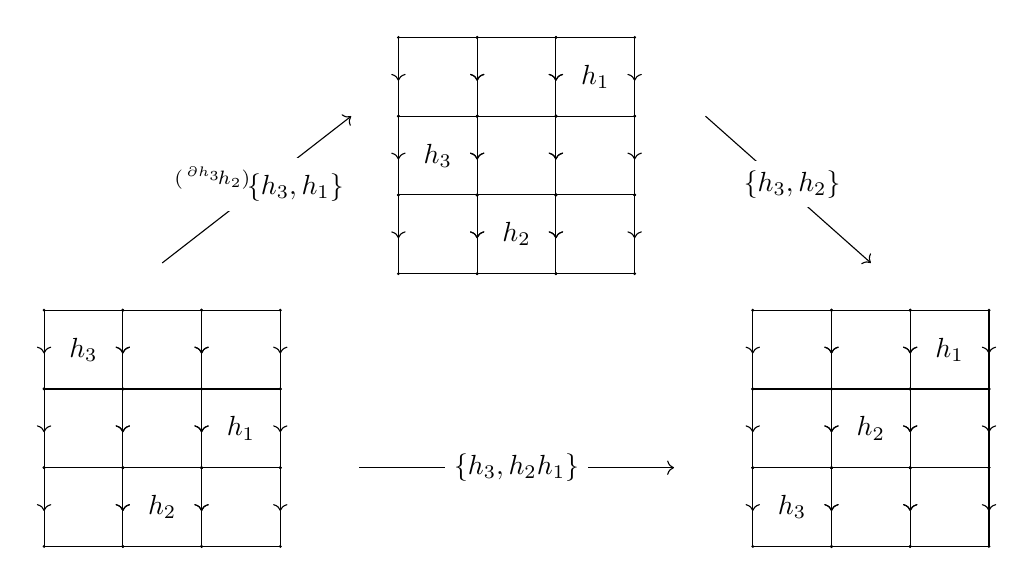
\begin{tikzpicture}[scale=1]
  	\begin{scope}[xshift=0.0cm]
	      \draw (0,0) to node[sloped] {\tikz{\draw[->](0,0)--(0.1,0);}} (0,-1);
	      \draw (1,0) to node[sloped] {\tikz{\draw[->](0,0)--(0.1,0);}} (1,-1);
	      \draw (0,0) to node[sloped] {\tikz{\draw[-](0,0)--(0.1,0);}} (1,0);
	      \draw (0,-1) to node  {\tikz{\draw[-](0,0)--(0.1,0);}} (1,-1);
	      \node at (1/2,-1/2) {$h_3$};
	      \draw (0,0) to node {\tikz{\draw[-](0,0)--(0.1,0);}}(1,0);
	      \draw (0,-1) to node {\tikz{\draw[-](0,0)--(0.1,0);}} (1,-1);
	      \fill[black] (0,0) circle[radius=0.02];
	      \fill[black] (1,0) circle[radius=0.02];
	      \fill[black] (0,-1) circle[radius=0.02];
	      \fill[black] (1,-1) circle[radius=0.02];
	    \begin{scope}[xshift=1.0cm]
	      \draw (0,0) to node[sloped] {\tikz{\draw[->](0,0)--(0.1,0);}} (0,-1);
	      \draw (1,0) to node[sloped] {\tikz{\draw[->](0,0)--(0.1,0);}} (1,-1);
	      \draw (0,0) to node[sloped] {\tikz{\draw[-](0,0)--(0.1,0);}} (1,0);
	      \draw (0,-1) to node  {\tikz{\draw[-](0,0)--(0.1,0);}} (1,-1);
	      \node at (1/2,-1/2) {$$};
	      \draw (0,0) to node {\tikz{\draw[-](0,0)--(0.1,0);}} (1,0);
	      \draw (0,-1) to node {\tikz{\draw[-](0,0)--(0.1,0);}} (1,-1);
	      \fill[black] (0,0) circle[radius=0.02];
	      \fill[black] (1,0) circle[radius=0.02];
	      \fill[black] (0,-1) circle[radius=0.02];
	      \fill[black] (1,-1) circle[radius=0.02];
	    \end{scope}
	    	 \begin{scope}[xshift=2.0cm]
	      \draw (0,0) to node[sloped] {\tikz{\draw[->](0,0)--(0.1,0);}} (0,-1);
	      \draw (1,0) to node[sloped] {\tikz{\draw[->](0,0)--(0.1,0);}} (1,-1);
	      \draw (0,0) to node[sloped] {\tikz{\draw[-](0,0)--(0.1,0);}} (1,0);
	      \draw (0,-1) to node  {\tikz{\draw[-](0,0)--(0.1,0);}} (1,-1);
	      \node at (1/2,-1/2) {$$};
	      \draw (0,0) to node {\tikz{\draw[-](0,0)--(0.1,0);}} (1,0);
	      \draw (0,-1) to node {\tikz{\draw[-](0,0)--(0.1,0);}} (1,-1);
	      \fill[black] (0,0) circle[radius=0.02];
	      \fill[black] (1,0) circle[radius=0.02];
	      \fill[black] (0,-1) circle[radius=0.02];
	      \fill[black] (1,-1) circle[radius=0.02];
	    \end{scope}
	        \begin{scope}[xshift=0.0cm, yshift = -1.0cm]
	      \draw (0,0) to node[sloped] {\tikz{\draw[->](0,0)--(0.1,0);}} (0,-1);
	      \draw (1,0) to node[sloped] {\tikz{\draw[->](0,0)--(0.1,0);}} (1,-1);
	      \draw (0,0) to node[sloped] {\tikz{\draw[-](0,0)--(0.1,0);}} (1,0);
	      \draw (0,-1) to node  {\tikz{\draw[-](0,0)--(0.1,0);}} (1,-1);
	      \node at (1/2,-1/2) {$$};
	      \draw (0,0) to node {\tikz{\draw[-](0,0)--(0.1,0);}} (1,0);
	      \draw (0,-1) to node {\tikz{\draw[-](0,0)--(0.1,0);}} (1,-1);
	      \fill[black] (0,0) circle[radius=0.02];
	      \fill[black] (1,0) circle[radius=0.02];
	      \fill[black] (0,-1) circle[radius=0.02];
	      \fill[black] (1,-1) circle[radius=0.02];
	    \end{scope}
	    \begin{scope}[xshift=1.0cm, yshift = -1.0cm]
	      \draw (0,0) to node[sloped] {\tikz{\draw[->](0,0)--(0.1,0);}} (0,-1);
	      \draw (1,0) to node[sloped] {\tikz{\draw[->](0,0)--(0.1,0);}} (1,-1);
	      \draw (0,0) to node[sloped] {\tikz{\draw[-](0,0)--(0.1,0);}} (1,0);
	      \draw (0,-1) to node  {\tikz{\draw[-](0,0)--(0.1,0);}} (1,-1);
	      \node at (1/2,-1/2) {$$};
	      \draw (0,0) to node {\tikz{\draw[-](0,0)--(0.1,0);}} (1,0);
	      \draw (0,-1) to node {\tikz{\draw[-](0,0)--(0.1,0);}} (1,-1);
	      \fill[black] (0,0) circle[radius=0.02];
	      \fill[black] (1,0) circle[radius=0.02];
	      \fill[black] (0,-1) circle[radius=0.02];
	      \fill[black] (1,-1) circle[radius=0.02];
	    \end{scope}
	     \begin{scope}[xshift=2.0cm, yshift = -1.0cm]
	      \draw (0,0) to node[sloped] {\tikz{\draw[->](0,0)--(0.1,0);}} (0,-1);
	      \draw (1,0) to node[sloped] {\tikz{\draw[->](0,0)--(0.1,0);}} (1,-1);
	      \draw (0,0) to node[sloped] {\tikz{\draw[-](0,0)--(0.1,0);}} (1,0);
	      \draw (0,-1) to node  {\tikz{\draw[-](0,0)--(0.1,0);}} (1,-1);
	      \node at (1/2,-1/2) {$h_1$};
	      \draw (0,0) to node {\tikz{\draw[-](0,0)--(0.1,0);}} (1,0);
	      \draw (0,-1) to node {\tikz{\draw[-](0,0)--(0.1,0);}} (1,-1);
	      \fill[black] (0,0) circle[radius=0.02];
	      \fill[black] (1,0) circle[radius=0.02];
	      \fill[black] (0,-1) circle[radius=0.02];
	      \fill[black] (1,-1) circle[radius=0.02];
	    \end{scope}
	     \begin{scope}[xshift=0.0cm, yshift = -2.0cm]
	      \draw (0,0) to node[sloped] {\tikz{\draw[->](0,0)--(0.1,0);}} (0,-1);
	      \draw (1,0) to node[sloped] {\tikz{\draw[->](0,0)--(0.1,0);}} (1,-1);
	      \draw (0,0) to node[sloped] {\tikz{\draw[-](0,0)--(0.1,0);}} (1,0);
	      \draw (0,-1) to node  {\tikz{\draw[-](0,0)--(0.1,0);}} (1,-1);
	      \node at (1/2,-1/2) {$$};
	      \draw (0,0) to node {\tikz{\draw[-](0,0)--(0.1,0);}} (1,0);
	      \draw (0,-1) to node {\tikz{\draw[-](0,0)--(0.1,0);}} (1,-1);
	      \fill[black] (0,0) circle[radius=0.02];
	      \fill[black] (1,0) circle[radius=0.02];
	      \fill[black] (0,-1) circle[radius=0.02];
	      \fill[black] (1,-1) circle[radius=0.02];
	    \end{scope}
	    \begin{scope}[xshift=1.0cm, yshift = -2.0cm]
	      \draw (0,0) to node[sloped] {\tikz{\draw[->](0,0)--(0.1,0);}} (0,-1);
	      \draw (1,0) to node[sloped] {\tikz{\draw[->](0,0)--(0.1,0);}} (1,-1);
	      \draw (0,0) to node[sloped] {\tikz{\draw[-](0,0)--(0.1,0);}} (1,0);
	      \draw (0,-1) to node  {\tikz{\draw[-](0,0)--(0.1,0);}} (1,-1);
	      \node at (1/2,-1/2) {$h_2$};
	      \draw (0,0) to node {\tikz{\draw[-](0,0)--(0.1,0);}}(1,0);
	      \draw (0,-1) to node {\tikz{\draw[-](0,0)--(0.1,0);}} (1,-1);
	      \fill[black] (0,0) circle[radius=0.02];
	      \fill[black] (1,0) circle[radius=0.02];
	      \fill[black] (0,-1) circle[radius=0.02];
	      \fill[black] (1,-1) circle[radius=0.02];
	    \end{scope}
	     \begin{scope}[xshift=2.0cm, yshift = -2.0cm]
	      \draw (0,0) to node[sloped] {\tikz{\draw[->](0,0)--(0.1,0);}} (0,-1);
	      \draw (1,0) to node[sloped] {\tikz{\draw[->](0,0)--(0.1,0);}} (1,-1);
	      \draw (0,0) to node[sloped] {\tikz{\draw[-](0,0)--(0.1,0);}} (1,0);
	      \draw (0,-1) to node  {\tikz{\draw[-](0,0)--(0.1,0);}} (1,-1);
	      \node at (1/2,-1/2) {$$};
	      \draw (0,0) to node {\tikz{\draw[-](0,0)--(0.1,0);}}(1,0);
	      \draw (0,-1) to node {\tikz{\draw[-](0,0)--(0.1,0);}} (1,-1);
	      \fill[black] (0,0) circle[radius=0.02];
	      \fill[black] (1,0) circle[radius=0.02];
	      \fill[black] (0,-1) circle[radius=0.02];
	      \fill[black] (1,-1) circle[radius=0.02];
	    \end{scope}
    \end{scope}
    \begin{scope}[xshift=4.5cm, yshift = 2*1.732cm]
	      \draw (0,0) to node[sloped] {\tikz{\draw[->](0,0)--(0.1,0);}} (0,-1);
	      \draw (1,0) to node[sloped] {\tikz{\draw[->](0,0)--(0.1,0);}} (1,-1);
	      \draw (0,0) to node[sloped] {\tikz{\draw[-](0,0)--(0.1,0);}} (1,0);
	      \draw (0,-1) to node  {\tikz{\draw[-](0,0)--(0.1,0);}} (1,-1);
	      \node at (1/2,-1/2) {$$};
	      \draw (0,0) to node {\tikz{\draw[-](0,0)--(0.1,0);}}(1,0);
	      \draw (0,-1) to node {\tikz{\draw[-](0,0)--(0.1,0);}} (1,-1);
	      \fill[black] (0,0) circle[radius=0.02];
	      \fill[black] (1,0) circle[radius=0.02];
	      \fill[black] (0,-1) circle[radius=0.02];
	      \fill[black] (1,-1) circle[radius=0.02];
	    \begin{scope}[xshift=1.0cm]
	      \draw (0,0) to node[sloped] {\tikz{\draw[->](0,0)--(0.1,0);}} (0,-1);
	      \draw (1,0) to node[sloped] {\tikz{\draw[->](0,0)--(0.1,0);}} (1,-1);
	      \draw (0,0) to node[sloped] {\tikz{\draw[-](0,0)--(0.1,0);}} (1,0);
	      \draw (0,-1) to node  {\tikz{\draw[-](0,0)--(0.1,0);}} (1,-1);
	      \node at (1/2,-1/2) {$$};
	      \draw (0,0) to node {\tikz{\draw[-](0,0)--(0.1,0);}} (1,0);
	      \draw (0,-1) to node {\tikz{\draw[-](0,0)--(0.1,0);}} (1,-1);
	      \fill[black] (0,0) circle[radius=0.02];
	      \fill[black] (1,0) circle[radius=0.02];
	      \fill[black] (0,-1) circle[radius=0.02];
	      \fill[black] (1,-1) circle[radius=0.02];
	    \end{scope}
	    	 \begin{scope}[xshift=2.0cm]
	      \draw (0,0) to node[sloped] {\tikz{\draw[->](0,0)--(0.1,0);}} (0,-1);
	      \draw (1,0) to node[sloped] {\tikz{\draw[->](0,0)--(0.1,0);}} (1,-1);
	      \draw (0,0) to node[sloped] {\tikz{\draw[-](0,0)--(0.1,0);}} (1,0);
	      \draw (0,-1) to node  {\tikz{\draw[-](0,0)--(0.1,0);}} (1,-1);
	      \node at (1/2,-1/2) {$h_1$};
	      \draw (0,0) to node {\tikz{\draw[-](0,0)--(0.1,0);}} (1,0);
	      \draw (0,-1) to node {\tikz{\draw[-](0,0)--(0.1,0);}} (1,-1);
	      \fill[black] (0,0) circle[radius=0.02];
	      \fill[black] (1,0) circle[radius=0.02];
	      \fill[black] (0,-1) circle[radius=0.02];
	      \fill[black] (1,-1) circle[radius=0.02];
	    \end{scope}
	        \begin{scope}[xshift=0.0cm, yshift = -1.0cm]
	      \draw (0,0) to node[sloped] {\tikz{\draw[->](0,0)--(0.1,0);}} (0,-1);
	      \draw (1,0) to node[sloped] {\tikz{\draw[->](0,0)--(0.1,0);}} (1,-1);
	      \draw (0,0) to node[sloped] {\tikz{\draw[-](0,0)--(0.1,0);}} (1,0);
	      \draw (0,-1) to node  {\tikz{\draw[-](0,0)--(0.1,0);}} (1,-1);
	      \node at (1/2,-1/2) {$h_3$};
	      \draw (0,0) to node {\tikz{\draw[-](0,0)--(0.1,0);}} (1,0);
	      \draw (0,-1) to node {\tikz{\draw[-](0,0)--(0.1,0);}} (1,-1);
	      \fill[black] (0,0) circle[radius=0.02];
	      \fill[black] (1,0) circle[radius=0.02];
	      \fill[black] (0,-1) circle[radius=0.02];
	      \fill[black] (1,-1) circle[radius=0.02];
	    \end{scope}
	    \begin{scope}[xshift=1.0cm, yshift = -1.0cm]
	      \draw (0,0) to node[sloped] {\tikz{\draw[->](0,0)--(0.1,0);}} (0,-1);
	      \draw (1,0) to node[sloped] {\tikz{\draw[->](0,0)--(0.1,0);}} (1,-1);
	      \draw (0,0) to node[sloped] {\tikz{\draw[-](0,0)--(0.1,0);}} (1,0);
	      \draw (0,-1) to node  {\tikz{\draw[-](0,0)--(0.1,0);}} (1,-1);
	      \node at (1/2,-1/2) {$$};
	      \draw (0,0) to node {\tikz{\draw[-](0,0)--(0.1,0);}} (1,0);
	      \draw (0,-1) to node {\tikz{\draw[-](0,0)--(0.1,0);}} (1,-1);
	      \fill[black] (0,0) circle[radius=0.02];
	      \fill[black] (1,0) circle[radius=0.02];
	      \fill[black] (0,-1) circle[radius=0.02];
	      \fill[black] (1,-1) circle[radius=0.02];
	    \end{scope}
	     \begin{scope}[xshift=2.0cm, yshift = -1.0cm]
	      \draw (0,0) to node[sloped] {\tikz{\draw[->](0,0)--(0.1,0);}} (0,-1);
	      \draw (1,0) to node[sloped] {\tikz{\draw[->](0,0)--(0.1,0);}} (1,-1);
	      \draw (0,0) to node[sloped] {\tikz{\draw[-](0,0)--(0.1,0);}} (1,0);
	      \draw (0,-1) to node  {\tikz{\draw[-](0,0)--(0.1,0);}} (1,-1);
	      \node at (1/2,-1/2) {$$};
	      \draw (0,0) to node {\tikz{\draw[-](0,0)--(0.1,0);}} (1,0);
	      \draw (0,-1) to node {\tikz{\draw[-](0,0)--(0.1,0);}} (1,-1);
	      \fill[black] (0,0) circle[radius=0.02];
	      \fill[black] (1,0) circle[radius=0.02];
	      \fill[black] (0,-1) circle[radius=0.02];
	      \fill[black] (1,-1) circle[radius=0.02];
	    \end{scope}
	     \begin{scope}[xshift=0.0cm, yshift = -2.0cm]
	      \draw (0,0) to node[sloped] {\tikz{\draw[->](0,0)--(0.1,0);}} (0,-1);
	      \draw (1,0) to node[sloped] {\tikz{\draw[->](0,0)--(0.1,0);}} (1,-1);
	      \draw (0,0) to node[sloped] {\tikz{\draw[-](0,0)--(0.1,0);}} (1,0);
	      \draw (0,-1) to node  {\tikz{\draw[-](0,0)--(0.1,0);}} (1,-1);
	      \node at (1/2,-1/2) {$$};
	      \draw (0,0) to node {\tikz{\draw[-](0,0)--(0.1,0);}} (1,0);
	      \draw (0,-1) to node {\tikz{\draw[-](0,0)--(0.1,0);}} (1,-1);
	      \fill[black] (0,0) circle[radius=0.02];
	      \fill[black] (1,0) circle[radius=0.02];
	      \fill[black] (0,-1) circle[radius=0.02];
	      \fill[black] (1,-1) circle[radius=0.02];
	    \end{scope}
	    \begin{scope}[xshift=1.0cm, yshift = -2.0cm]
	      \draw (0,0) to node[sloped] {\tikz{\draw[->](0,0)--(0.1,0);}} (0,-1);
	      \draw (1,0) to node[sloped] {\tikz{\draw[->](0,0)--(0.1,0);}} (1,-1);
	      \draw (0,0) to node[sloped] {\tikz{\draw[-](0,0)--(0.1,0);}} (1,0);
	      \draw (0,-1) to node  {\tikz{\draw[-](0,0)--(0.1,0);}} (1,-1);
	      \node at (1/2,-1/2) {$h_2$};
	      \draw (0,0) to node {\tikz{\draw[-](0,0)--(0.1,0);}}(1,0);
	      \draw (0,-1) to node {\tikz{\draw[-](0,0)--(0.1,0);}} (1,-1);
	      \fill[black] (0,0) circle[radius=0.02];
	      \fill[black] (1,0) circle[radius=0.02];
	      \fill[black] (0,-1) circle[radius=0.02];
	      \fill[black] (1,-1) circle[radius=0.02];
	    \end{scope}
	     \begin{scope}[xshift=2.0cm, yshift = -2.0cm]
	      \draw (0,0) to node[sloped] {\tikz{\draw[->](0,0)--(0.1,0);}} (0,-1);
	      \draw (1,0) to node[sloped] {\tikz{\draw[->](0,0)--(0.1,0);}} (1,-1);
	      \draw (0,0) to node[sloped] {\tikz{\draw[-](0,0)--(0.1,0);}} (1,0);
	      \draw (0,-1) to node  {\tikz{\draw[-](0,0)--(0.1,0);}} (1,-1);
	      \node at (1/2,-1/2) {$$};
	      \draw (0,0) to node {\tikz{\draw[-](0,0)--(0.1,0);}}(1,0);
	      \draw (0,-1) to node {\tikz{\draw[-](0,0)--(0.1,0);}} (1,-1);
	      \fill[black] (0,0) circle[radius=0.02];
	      \fill[black] (1,0) circle[radius=0.02];
	      \fill[black] (0,-1) circle[radius=0.02];
	      \fill[black] (1,-1) circle[radius=0.02];
	    \end{scope}
    \end{scope}
    \begin{scope}[xshift=9.0cm]
	      \draw (0,0) to node[sloped] {\tikz{\draw[->](0,0)--(0.1,0);}} (0,-1);
	      \draw (1,0) to node[sloped] {\tikz{\draw[->](0,0)--(0.1,0);}} (1,-1);
	      \draw (0,0) to node[sloped] {\tikz{\draw[-](0,0)--(0.1,0);}} (1,0);
	      \draw (0,-1) to node  {\tikz{\draw[-](0,0)--(0.1,0);}} (1,-1);
	      \node at (1/2,-1/2) {$$};
	      \draw (0,0) to node {\tikz{\draw[-](0,0)--(0.1,0);}}(1,0);
	      \draw (0,-1) to node {\tikz{\draw[-](0,0)--(0.1,0);}} (1,-1);
	      \fill[black] (0,0) circle[radius=0.02];
	      \fill[black] (1,0) circle[radius=0.02];
	      \fill[black] (0,-1) circle[radius=0.02];
	      \fill[black] (1,-1) circle[radius=0.02];
	    \begin{scope}[xshift=1.0cm]
	      \draw (0,0) to node[sloped] {\tikz{\draw[->](0,0)--(0.1,0);}} (0,-1);
	      \draw (1,0) to node[sloped] {\tikz{\draw[->](0,0)--(0.1,0);}} (1,-1);
	      \draw (0,0) to node[sloped] {\tikz{\draw[-](0,0)--(0.1,0);}} (1,0);
	      \draw (0,-1) to node  {\tikz{\draw[-](0,0)--(0.1,0);}} (1,-1);
	      \node at (1/2,-1/2) {$$};
	      \draw (0,0) to node {\tikz{\draw[-](0,0)--(0.1,0);}} (1,0);
	      \draw (0,-1) to node {\tikz{\draw[-](0,0)--(0.1,0);}} (1,-1);
	      \fill[black] (0,0) circle[radius=0.02];
	      \fill[black] (1,0) circle[radius=0.02];
	      \fill[black] (0,-1) circle[radius=0.02];
	      \fill[black] (1,-1) circle[radius=0.02];
	    \end{scope}
	    	 \begin{scope}[xshift=2.0cm]
	      \draw (0,0) to node[sloped] {\tikz{\draw[->](0,0)--(0.1,0);}} (0,-1);
	      \draw (1,0) to node[sloped] {\tikz{\draw[->](0,0)--(0.1,0);}} (1,-1);
	      \draw (0,0) to node[sloped] {\tikz{\draw[-](0,0)--(0.1,0);}} (1,0);
	      \draw (0,-1) to node  {\tikz{\draw[-](0,0)--(0.1,0);}} (1,-1);
	      \node at (1/2,-1/2) {$h_1$};
	      \draw (0,0) to node {\tikz{\draw[-](0,0)--(0.1,0);}} (1,0);
	      \draw (0,-1) to node {\tikz{\draw[-](0,0)--(0.1,0);}} (1,-1);
	      \fill[black] (0,0) circle[radius=0.02];
	      \fill[black] (1,0) circle[radius=0.02];
	      \fill[black] (0,-1) circle[radius=0.02];
	      \fill[black] (1,-1) circle[radius=0.02];
	    \end{scope}
	        \begin{scope}[xshift=0.0cm, yshift = -1.0cm]
	      \draw (0,0) to node[sloped] {\tikz{\draw[->](0,0)--(0.1,0);}} (0,-1);
	      \draw (1,0) to node[sloped] {\tikz{\draw[->](0,0)--(0.1,0);}} (1,-1);
	      \draw (0,0) to node[sloped] {\tikz{\draw[-](0,0)--(0.1,0);}} (1,0);
	      \draw (0,-1) to node  {\tikz{\draw[-](0,0)--(0.1,0);}} (1,-1);
	      \node at (1/2,-1/2) {$$};
	      \draw (0,0) to node {\tikz{\draw[-](0,0)--(0.1,0);}} (1,0);
	      \draw (0,-1) to node {\tikz{\draw[-](0,0)--(0.1,0);}} (1,-1);
	      \fill[black] (0,0) circle[radius=0.02];
	      \fill[black] (1,0) circle[radius=0.02];
	      \fill[black] (0,-1) circle[radius=0.02];
	      \fill[black] (1,-1) circle[radius=0.02];
	    \end{scope}
	    \begin{scope}[xshift=1.0cm, yshift = -1.0cm]
	      \draw (0,0) to node[sloped] {\tikz{\draw[->](0,0)--(0.1,0);}} (0,-1);
	      \draw (1,0) to node[sloped] {\tikz{\draw[->](0,0)--(0.1,0);}} (1,-1);
	      \draw (0,0) to node[sloped] {\tikz{\draw[-](0,0)--(0.1,0);}} (1,0);
	      \draw (0,-1) to node  {\tikz{\draw[-](0,0)--(0.1,0);}} (1,-1);
	      \node at (1/2,-1/2) {$h_2$};
	      \draw (0,0) to node {\tikz{\draw[-](0,0)--(0.1,0);}} (1,0);
	      \draw (0,-1) to node {\tikz{\draw[-](0,0)--(0.1,0);}} (1,-1);
	      \fill[black] (0,0) circle[radius=0.02];
	      \fill[black] (1,0) circle[radius=0.02];
	      \fill[black] (0,-1) circle[radius=0.02];
	      \fill[black] (1,-1) circle[radius=0.02];
	    \end{scope}
	     \begin{scope}[xshift=2.0cm, yshift = -1.0cm]
	      \draw (0,0) to node[sloped] {\tikz{\draw[->](0,0)--(0.1,0);}} (0,-1);
	      \draw (1,0) to node[sloped] {\tikz{\draw[->](0,0)--(0.1,0);}} (1,-1);
	      \draw (0,0) to node[sloped] {\tikz{\draw[-](0,0)--(0.1,0);}} (1,0);
	      \draw (0,-1) to node  {\tikz{\draw[-](0,0)--(0.1,0);}} (1,-1);
	      \node at (1/2,-1/2) {$$};
	      \draw (0,0) to node {\tikz{\draw[-](0,0)--(0.1,0);}} (1,0);
	      \draw (0,-1) to node {\tikz{\draw[-](0,0)--(0.1,0);}} (1,-1);
	      \fill[black] (0,0) circle[radius=0.02];
	      \fill[black] (1,0) circle[radius=0.02];
	      \fill[black] (0,-1) circle[radius=0.02];
	      \fill[black] (1,-1) circle[radius=0.02];
	    \end{scope}
	     \begin{scope}[xshift=0.0cm, yshift = -2.0cm]
	      \draw (0,0) to node[sloped] {\tikz{\draw[->](0,0)--(0.1,0);}} (0,-1);
	      \draw (1,0) to node[sloped] {\tikz{\draw[->](0,0)--(0.1,0);}} (1,-1);
	      \draw (0,0) to node[sloped] {\tikz{\draw[-](0,0)--(0.1,0);}} (1,0);
	      \draw (0,-1) to node  {\tikz{\draw[-](0,0)--(0.1,0);}} (1,-1);
	      \node at (1/2,-1/2) {$h_3$};
	      \draw (0,0) to node {\tikz{\draw[-](0,0)--(0.1,0);}} (1,0);
	      \draw (0,-1) to node {\tikz{\draw[-](0,0)--(0.1,0);}} (1,-1);
	      \fill[black] (0,0) circle[radius=0.02];
	      \fill[black] (1,0) circle[radius=0.02];
	      \fill[black] (0,-1) circle[radius=0.02];
	      \fill[black] (1,-1) circle[radius=0.02];
	    \end{scope}
	    \begin{scope}[xshift=1.0cm, yshift = -2.0cm]
	      \draw (0,0) to node[sloped] {\tikz{\draw[->](0,0)--(0.1,0);}} (0,-1);
	      \draw (1,0) to node[sloped] {\tikz{\draw[->](0,0)--(0.1,0);}} (1,-1);
	      \draw (0,0) to node[sloped] {\tikz{\draw[-](0,0)--(0.1,0);}} (1,0);
	      \draw (0,-1) to node  {\tikz{\draw[-](0,0)--(0.1,0);}} (1,-1);
	      \node at (1/2,-1/2) {$$};
	      \draw (0,0) to node {\tikz{\draw[-](0,0)--(0.1,0);}}(1,0);
	      \draw (0,-1) to node {\tikz{\draw[-](0,0)--(0.1,0);}} (1,-1);
	      \fill[black] (0,0) circle[radius=0.02];
	      \fill[black] (1,0) circle[radius=0.02];
	      \fill[black] (0,-1) circle[radius=0.02];
	      \fill[black] (1,-1) circle[radius=0.02];
	    \end{scope}
	     \begin{scope}[xshift=2.0cm, yshift = -2.0cm]
	      \draw (0,0) to node[sloped] {\tikz{\draw[->](0,0)--(0.1,0);}} (0,-1);
	      \draw (1,0) to node[sloped] {\tikz{\draw[->](0,0)--(0.1,0);}} (1,-1);
	      \draw (0,0) to node[sloped] {\tikz{\draw[-](0,0)--(0.1,0);}} (1,0);
	      \draw (0,-1) to node  {\tikz{\draw[-](0,0)--(0.1,0);}} (1,-1);
	      \node at (1/2,-1/2) {$$};
	      \draw (0,0) to node {\tikz{\draw[-](0,0)--(0.1,0);}}(1,0);
	      \draw (0,-1) to node {\tikz{\draw[-](0,0)--(0.1,0);}} (1,-1);
	      \fill[black] (0,0) circle[radius=0.02];
	      \fill[black] (1,0) circle[radius=0.02];
	      \fill[black] (0,-1) circle[radius=0.02];
	      \fill[black] (1,-1) circle[radius=0.02];
	    \end{scope}
    \end{scope}
     \draw[->] (4,-2) to (8,-2);
      \node at (6,-2) [fill=white]{$\{h_3 ,h_2 h_1\}$};
       \draw[->] (1.5 , 0.1+1/2) to (4.4-1/2,-1+ 2*1.732);
      \node at (2.7,1.6) [fill=white]{$\act{(\act{\del h_3}h_2)}\{h_3, h_1 \}$};
       \draw[->](3+4.4+1,-1+ 2*1.732) to (10.5, 0.6);
      \node at (9.5,1.6)  [fill=white]{$\{h_3, h_2\}$};
  \end{tikzpicture}
\end{center}
\caption{Figure of property \ref{rpl} of 2-crossed module}
\label{d:PF_lift_right}
\end{figure}

Property~\ref{pfeq} of 2-crossed module, i.e. $\act{g}\{h_2, h_1\} = \{\act{g}h_2, \act{g} h_1\}$ for $g\in G$ and $h_1,h_2\in H$ guarantees that the diagram is well-defined. Let $h_1,h_2,h_3\in H$. We now consider Figure~\ref{d:PF_lift_wd}.
\begin{figure}
\begin{center}
  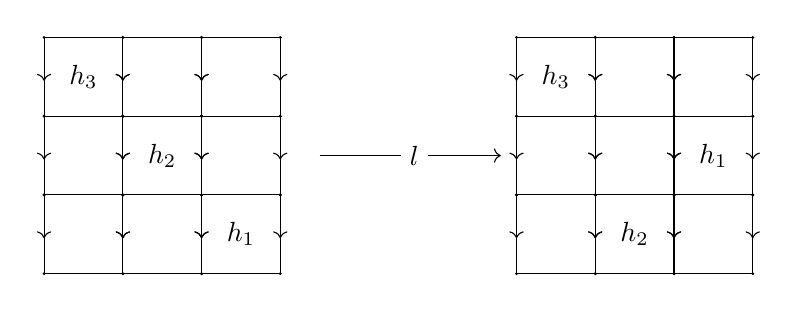
\begin{tikzpicture}[scale=1]
  	\begin{scope}[xshift=0.0cm]
	      \draw (0,0) to node[sloped] {\tikz{\draw[->](0,0)--(0.1,0);}} (0,-1);
	      \draw (1,0) to node[sloped] {\tikz{\draw[->](0,0)--(0.1,0);}} (1,-1);
	      \draw (0,0) to node[sloped] {\tikz{\draw[-](0,0)--(0.1,0);}} (1,0);
	      \draw (0,-1) to node  {\tikz{\draw[-](0,0)--(0.1,0);}} (1,-1);
	      \node at (1/2,-1/2) {$h_3$};
	      \draw (0,0) to node {\tikz{\draw[-](0,0)--(0.1,0);}}(1,0);
	      \draw (0,-1) to node {\tikz{\draw[-](0,0)--(0.1,0);}} (1,-1);
	      \fill[black] (0,0) circle[radius=0.02];
	      \fill[black] (1,0) circle[radius=0.02];
	      \fill[black] (0,-1) circle[radius=0.02];
	      \fill[black] (1,-1) circle[radius=0.02];
	    \begin{scope}[xshift=1.0cm]
	      \draw (0,0) to node[sloped] {\tikz{\draw[->](0,0)--(0.1,0);}} (0,-1);
	      \draw (1,0) to node[sloped] {\tikz{\draw[->](0,0)--(0.1,0);}} (1,-1);
	      \draw (0,0) to node[sloped] {\tikz{\draw[-](0,0)--(0.1,0);}} (1,0);
	      \draw (0,-1) to node  {\tikz{\draw[-](0,0)--(0.1,0);}} (1,-1);
	      \node at (1/2,-1/2) {$$};
	      \draw (0,0) to node {\tikz{\draw[-](0,0)--(0.1,0);}} (1,0);
	      \draw (0,-1) to node {\tikz{\draw[-](0,0)--(0.1,0);}} (1,-1);
	      \fill[black] (0,0) circle[radius=0.02];
	      \fill[black] (1,0) circle[radius=0.02];
	      \fill[black] (0,-1) circle[radius=0.02];
	      \fill[black] (1,-1) circle[radius=0.02];
	    \end{scope}
	    	 \begin{scope}[xshift=2.0cm]
	      \draw (0,0) to node[sloped] {\tikz{\draw[->](0,0)--(0.1,0);}} (0,-1);
	      \draw (1,0) to node[sloped] {\tikz{\draw[->](0,0)--(0.1,0);}} (1,-1);
	      \draw (0,0) to node[sloped] {\tikz{\draw[-](0,0)--(0.1,0);}} (1,0);
	      \draw (0,-1) to node  {\tikz{\draw[-](0,0)--(0.1,0);}} (1,-1);
	      \node at (1/2,-1/2) {$$};
	      \draw (0,0) to node {\tikz{\draw[-](0,0)--(0.1,0);}} (1,0);
	      \draw (0,-1) to node {\tikz{\draw[-](0,0)--(0.1,0);}} (1,-1);
	      \fill[black] (0,0) circle[radius=0.02];
	      \fill[black] (1,0) circle[radius=0.02];
	      \fill[black] (0,-1) circle[radius=0.02];
	      \fill[black] (1,-1) circle[radius=0.02];
	    \end{scope}
	        \begin{scope}[xshift=0.0cm, yshift = -1.0cm]
	      \draw (0,0) to node[sloped] {\tikz{\draw[->](0,0)--(0.1,0);}} (0,-1);
	      \draw (1,0) to node[sloped] {\tikz{\draw[->](0,0)--(0.1,0);}} (1,-1);
	      \draw (0,0) to node[sloped] {\tikz{\draw[-](0,0)--(0.1,0);}} (1,0);
	      \draw (0,-1) to node  {\tikz{\draw[-](0,0)--(0.1,0);}} (1,-1);
	      \node at (1/2,-1/2) {$$};
	      \draw (0,0) to node {\tikz{\draw[-](0,0)--(0.1,0);}} (1,0);
	      \draw (0,-1) to node {\tikz{\draw[-](0,0)--(0.1,0);}} (1,-1);
	      \fill[black] (0,0) circle[radius=0.02];
	      \fill[black] (1,0) circle[radius=0.02];
	      \fill[black] (0,-1) circle[radius=0.02];
	      \fill[black] (1,-1) circle[radius=0.02];
	    \end{scope}
	    \begin{scope}[xshift=1.0cm, yshift = -1.0cm]
	      \draw (0,0) to node[sloped] {\tikz{\draw[->](0,0)--(0.1,0);}} (0,-1);
	      \draw (1,0) to node[sloped] {\tikz{\draw[->](0,0)--(0.1,0);}} (1,-1);
	      \draw (0,0) to node[sloped] {\tikz{\draw[-](0,0)--(0.1,0);}} (1,0);
	      \draw (0,-1) to node  {\tikz{\draw[-](0,0)--(0.1,0);}} (1,-1);
	      \node at (1/2,-1/2) {$h_2$};
	      \draw (0,0) to node {\tikz{\draw[-](0,0)--(0.1,0);}} (1,0);
	      \draw (0,-1) to node {\tikz{\draw[-](0,0)--(0.1,0);}} (1,-1);
	      \fill[black] (0,0) circle[radius=0.02];
	      \fill[black] (1,0) circle[radius=0.02];
	      \fill[black] (0,-1) circle[radius=0.02];
	      \fill[black] (1,-1) circle[radius=0.02];
	    \end{scope}
	     \begin{scope}[xshift=2.0cm, yshift = -1.0cm]
	      \draw (0,0) to node[sloped] {\tikz{\draw[->](0,0)--(0.1,0);}} (0,-1);
	      \draw (1,0) to node[sloped] {\tikz{\draw[->](0,0)--(0.1,0);}} (1,-1);
	      \draw (0,0) to node[sloped] {\tikz{\draw[-](0,0)--(0.1,0);}} (1,0);
	      \draw (0,-1) to node  {\tikz{\draw[-](0,0)--(0.1,0);}} (1,-1);
	      \node at (1/2,-1/2) {$$};
	      \draw (0,0) to node {\tikz{\draw[-](0,0)--(0.1,0);}} (1,0);
	      \draw (0,-1) to node {\tikz{\draw[-](0,0)--(0.1,0);}} (1,-1);
	      \fill[black] (0,0) circle[radius=0.02];
	      \fill[black] (1,0) circle[radius=0.02];
	      \fill[black] (0,-1) circle[radius=0.02];
	      \fill[black] (1,-1) circle[radius=0.02];
	    \end{scope}
	     \begin{scope}[xshift=0.0cm, yshift = -2.0cm]
	      \draw (0,0) to node[sloped] {\tikz{\draw[->](0,0)--(0.1,0);}} (0,-1);
	      \draw (1,0) to node[sloped] {\tikz{\draw[->](0,0)--(0.1,0);}} (1,-1);
	      \draw (0,0) to node[sloped] {\tikz{\draw[-](0,0)--(0.1,0);}} (1,0);
	      \draw (0,-1) to node  {\tikz{\draw[-](0,0)--(0.1,0);}} (1,-1);
	      \node at (1/2,-1/2) {$$};
	      \draw (0,0) to node {\tikz{\draw[-](0,0)--(0.1,0);}} (1,0);
	      \draw (0,-1) to node {\tikz{\draw[-](0,0)--(0.1,0);}} (1,-1);
	      \fill[black] (0,0) circle[radius=0.02];
	      \fill[black] (1,0) circle[radius=0.02];
	      \fill[black] (0,-1) circle[radius=0.02];
	      \fill[black] (1,-1) circle[radius=0.02];
	    \end{scope}
	    \begin{scope}[xshift=1.0cm, yshift = -2.0cm]
	      \draw (0,0) to node[sloped] {\tikz{\draw[->](0,0)--(0.1,0);}} (0,-1);
	      \draw (1,0) to node[sloped] {\tikz{\draw[->](0,0)--(0.1,0);}} (1,-1);
	      \draw (0,0) to node[sloped] {\tikz{\draw[-](0,0)--(0.1,0);}} (1,0);
	      \draw (0,-1) to node  {\tikz{\draw[-](0,0)--(0.1,0);}} (1,-1);
	      \node at (1/2,-1/2) {$$};
	      \draw (0,0) to node {\tikz{\draw[-](0,0)--(0.1,0);}}(1,0);
	      \draw (0,-1) to node {\tikz{\draw[-](0,0)--(0.1,0);}} (1,-1);
	      \fill[black] (0,0) circle[radius=0.02];
	      \fill[black] (1,0) circle[radius=0.02];
	      \fill[black] (0,-1) circle[radius=0.02];
	      \fill[black] (1,-1) circle[radius=0.02];
	    \end{scope}
	     \begin{scope}[xshift=2.0cm, yshift = -2.0cm]
	      \draw (0,0) to node[sloped] {\tikz{\draw[->](0,0)--(0.1,0);}} (0,-1);
	      \draw (1,0) to node[sloped] {\tikz{\draw[->](0,0)--(0.1,0);}} (1,-1);
	      \draw (0,0) to node[sloped] {\tikz{\draw[-](0,0)--(0.1,0);}} (1,0);
	      \draw (0,-1) to node  {\tikz{\draw[-](0,0)--(0.1,0);}} (1,-1);
	      \node at (1/2,-1/2) {$h_1$};
	      \draw (0,0) to node {\tikz{\draw[-](0,0)--(0.1,0);}}(1,0);
	      \draw (0,-1) to node {\tikz{\draw[-](0,0)--(0.1,0);}} (1,-1);
	      \fill[black] (0,0) circle[radius=0.02];
	      \fill[black] (1,0) circle[radius=0.02];
	      \fill[black] (0,-1) circle[radius=0.02];
	      \fill[black] (1,-1) circle[radius=0.02];
	    \end{scope}
    \end{scope}
    \begin{scope}[xshift=6cm]
	      \draw (0,0) to node[sloped] {\tikz{\draw[->](0,0)--(0.1,0);}} (0,-1);
	      \draw (1,0) to node[sloped] {\tikz{\draw[->](0,0)--(0.1,0);}} (1,-1);
	      \draw (0,0) to node[sloped] {\tikz{\draw[-](0,0)--(0.1,0);}} (1,0);
	      \draw (0,-1) to node  {\tikz{\draw[-](0,0)--(0.1,0);}} (1,-1);
	      \node at (1/2,-1/2) {$h_3$};
	      \draw (0,0) to node {\tikz{\draw[-](0,0)--(0.1,0);}}(1,0);
	      \draw (0,-1) to node {\tikz{\draw[-](0,0)--(0.1,0);}} (1,-1);
	      \fill[black] (0,0) circle[radius=0.02];
	      \fill[black] (1,0) circle[radius=0.02];
	      \fill[black] (0,-1) circle[radius=0.02];
	      \fill[black] (1,-1) circle[radius=0.02];
	    \begin{scope}[xshift=1.0cm]
	      \draw (0,0) to node[sloped] {\tikz{\draw[->](0,0)--(0.1,0);}} (0,-1);
	      \draw (1,0) to node[sloped] {\tikz{\draw[->](0,0)--(0.1,0);}} (1,-1);
	      \draw (0,0) to node[sloped] {\tikz{\draw[-](0,0)--(0.1,0);}} (1,0);
	      \draw (0,-1) to node  {\tikz{\draw[-](0,0)--(0.1,0);}} (1,-1);
	      \node at (1/2,-1/2) {$$};
	      \draw (0,0) to node {\tikz{\draw[-](0,0)--(0.1,0);}} (1,0);
	      \draw (0,-1) to node {\tikz{\draw[-](0,0)--(0.1,0);}} (1,-1);
	      \fill[black] (0,0) circle[radius=0.02];
	      \fill[black] (1,0) circle[radius=0.02];
	      \fill[black] (0,-1) circle[radius=0.02];
	      \fill[black] (1,-1) circle[radius=0.02];
	    \end{scope}
	    	 \begin{scope}[xshift=2.0cm]
	      \draw (0,0) to node[sloped] {\tikz{\draw[->](0,0)--(0.1,0);}} (0,-1);
	      \draw (1,0) to node[sloped] {\tikz{\draw[->](0,0)--(0.1,0);}} (1,-1);
	      \draw (0,0) to node[sloped] {\tikz{\draw[-](0,0)--(0.1,0);}} (1,0);
	      \draw (0,-1) to node  {\tikz{\draw[-](0,0)--(0.1,0);}} (1,-1);
	      \node at (1/2,-1/2) {$$};
	      \draw (0,0) to node {\tikz{\draw[-](0,0)--(0.1,0);}} (1,0);
	      \draw (0,-1) to node {\tikz{\draw[-](0,0)--(0.1,0);}} (1,-1);
	      \fill[black] (0,0) circle[radius=0.02];
	      \fill[black] (1,0) circle[radius=0.02];
	      \fill[black] (0,-1) circle[radius=0.02];
	      \fill[black] (1,-1) circle[radius=0.02];
	    \end{scope}
	        \begin{scope}[xshift=0.0cm, yshift = -1.0cm]
	      \draw (0,0) to node[sloped] {\tikz{\draw[->](0,0)--(0.1,0);}} (0,-1);
	      \draw (1,0) to node[sloped] {\tikz{\draw[->](0,0)--(0.1,0);}} (1,-1);
	      \draw (0,0) to node[sloped] {\tikz{\draw[-](0,0)--(0.1,0);}} (1,0);
	      \draw (0,-1) to node  {\tikz{\draw[-](0,0)--(0.1,0);}} (1,-1);
	      \node at (1/2,-1/2) {$$};
	      \draw (0,0) to node {\tikz{\draw[-](0,0)--(0.1,0);}} (1,0);
	      \draw (0,-1) to node {\tikz{\draw[-](0,0)--(0.1,0);}} (1,-1);
	      \fill[black] (0,0) circle[radius=0.02];
	      \fill[black] (1,0) circle[radius=0.02];
	      \fill[black] (0,-1) circle[radius=0.02];
	      \fill[black] (1,-1) circle[radius=0.02];
	    \end{scope}
	    \begin{scope}[xshift=1.0cm, yshift = -1.0cm]
	      \draw (0,0) to node[sloped] {\tikz{\draw[->](0,0)--(0.1,0);}} (0,-1);
	      \draw (1,0) to node[sloped] {\tikz{\draw[->](0,0)--(0.1,0);}} (1,-1);
	      \draw (0,0) to node[sloped] {\tikz{\draw[-](0,0)--(0.1,0);}} (1,0);
	      \draw (0,-1) to node  {\tikz{\draw[-](0,0)--(0.1,0);}} (1,-1);
	      \node at (1/2,-1/2) {$$};
	      \draw (0,0) to node {\tikz{\draw[-](0,0)--(0.1,0);}} (1,0);
	      \draw (0,-1) to node {\tikz{\draw[-](0,0)--(0.1,0);}} (1,-1);
	      \fill[black] (0,0) circle[radius=0.02];
	      \fill[black] (1,0) circle[radius=0.02];
	      \fill[black] (0,-1) circle[radius=0.02];
	      \fill[black] (1,-1) circle[radius=0.02];
	    \end{scope}
	     \begin{scope}[xshift=2.0cm, yshift = -1.0cm]
	      \draw (0,0) to node[sloped] {\tikz{\draw[->](0,0)--(0.1,0);}} (0,-1);
	      \draw (1,0) to node[sloped] {\tikz{\draw[->](0,0)--(0.1,0);}} (1,-1);
	      \draw (0,0) to node[sloped] {\tikz{\draw[-](0,0)--(0.1,0);}} (1,0);
	      \draw (0,-1) to node  {\tikz{\draw[-](0,0)--(0.1,0);}} (1,-1);
	      \node at (1/2,-1/2) {$h_1$};
	      \draw (0,0) to node {\tikz{\draw[-](0,0)--(0.1,0);}} (1,0);
	      \draw (0,-1) to node {\tikz{\draw[-](0,0)--(0.1,0);}} (1,-1);
	      \fill[black] (0,0) circle[radius=0.02];
	      \fill[black] (1,0) circle[radius=0.02];
	      \fill[black] (0,-1) circle[radius=0.02];
	      \fill[black] (1,-1) circle[radius=0.02];
	    \end{scope}
	     \begin{scope}[xshift=0.0cm, yshift = -2.0cm]
	      \draw (0,0) to node[sloped] {\tikz{\draw[->](0,0)--(0.1,0);}} (0,-1);
	      \draw (1,0) to node[sloped] {\tikz{\draw[->](0,0)--(0.1,0);}} (1,-1);
	      \draw (0,0) to node[sloped] {\tikz{\draw[-](0,0)--(0.1,0);}} (1,0);
	      \draw (0,-1) to node  {\tikz{\draw[-](0,0)--(0.1,0);}} (1,-1);
	      \node at (1/2,-1/2) {$$};
	      \draw (0,0) to node {\tikz{\draw[-](0,0)--(0.1,0);}} (1,0);
	      \draw (0,-1) to node {\tikz{\draw[-](0,0)--(0.1,0);}} (1,-1);
	      \fill[black] (0,0) circle[radius=0.02];
	      \fill[black] (1,0) circle[radius=0.02];
	      \fill[black] (0,-1) circle[radius=0.02];
	      \fill[black] (1,-1) circle[radius=0.02];
	    \end{scope}
	    \begin{scope}[xshift=1.0cm, yshift = -2.0cm]
	      \draw (0,0) to node[sloped] {\tikz{\draw[->](0,0)--(0.1,0);}} (0,-1);
	      \draw (1,0) to node[sloped] {\tikz{\draw[->](0,0)--(0.1,0);}} (1,-1);
	      \draw (0,0) to node[sloped] {\tikz{\draw[-](0,0)--(0.1,0);}} (1,0);
	      \draw (0,-1) to node  {\tikz{\draw[-](0,0)--(0.1,0);}} (1,-1);
	      \node at (1/2,-1/2) {$h_2$};
	      \draw (0,0) to node {\tikz{\draw[-](0,0)--(0.1,0);}}(1,0);
	      \draw (0,-1) to node {\tikz{\draw[-](0,0)--(0.1,0);}} (1,-1);
	      \fill[black] (0,0) circle[radius=0.02];
	      \fill[black] (1,0) circle[radius=0.02];
	      \fill[black] (0,-1) circle[radius=0.02];
	      \fill[black] (1,-1) circle[radius=0.02];
	    \end{scope}
	     \begin{scope}[xshift=2.0cm, yshift = -2.0cm]
	      \draw (0,0) to node[sloped] {\tikz{\draw[->](0,0)--(0.1,0);}} (0,-1);
	      \draw (1,0) to node[sloped] {\tikz{\draw[->](0,0)--(0.1,0);}} (1,-1);
	      \draw (0,0) to node[sloped] {\tikz{\draw[-](0,0)--(0.1,0);}} (1,0);
	      \draw (0,-1) to node  {\tikz{\draw[-](0,0)--(0.1,0);}} (1,-1);
	      \node at (1/2,-1/2) {$$};
	      \draw (0,0) to node {\tikz{\draw[-](0,0)--(0.1,0);}}(1,0);
	      \draw (0,-1) to node {\tikz{\draw[-](0,0)--(0.1,0);}} (1,-1);
	      \fill[black] (0,0) circle[radius=0.02];
	      \fill[black] (1,0) circle[radius=0.02];
	      \fill[black] (0,-1) circle[radius=0.02];
	      \fill[black] (1,-1) circle[radius=0.02];
	    \end{scope}
    \end{scope}
     \draw[->] (3.5,-1.5) to (5.8,-1.5);
      \node at (4.7,-1.5) [fill=white]{$l$};
  \end{tikzpicture}
\end{center}
\caption{Figure of property \ref{pfeq} of 2-crossed module}
\label{d:PF_lift_wd}
\end{figure}
From Figure~\ref{d:PF_lift_wd}, we can derive two different formulas. One is 
\[
l = {\rm id}_{{\rm id}_{\del(h_3)}} \#_1 \{h_2,h_1\} = \act{\del h_3} \{h_2,h_1\}.
\]
 The other is 
 \[
 l =\{{\rm id}_{\del(h_3)}\#_1 h_2, {\rm id}_{\del(h_3)} \#_1h_1 \} =\{\act{\del h_3}h_2,\act{\del h_3}h_1 \} .
 \]
  By Property~\ref{pfeq} of 2-crossed module, these two formulas are identical.

We can now interpret the two new operators in the 3-crossed module — the left-homannian and right-homannian — as illustrated in the diagrams. The left-homannian is a twisted version of Property~\ref{lpl} of 2-crossed module, and it is represented in Figure~\ref{d:lhmn}.
\begin{figure}
\begin{center}
  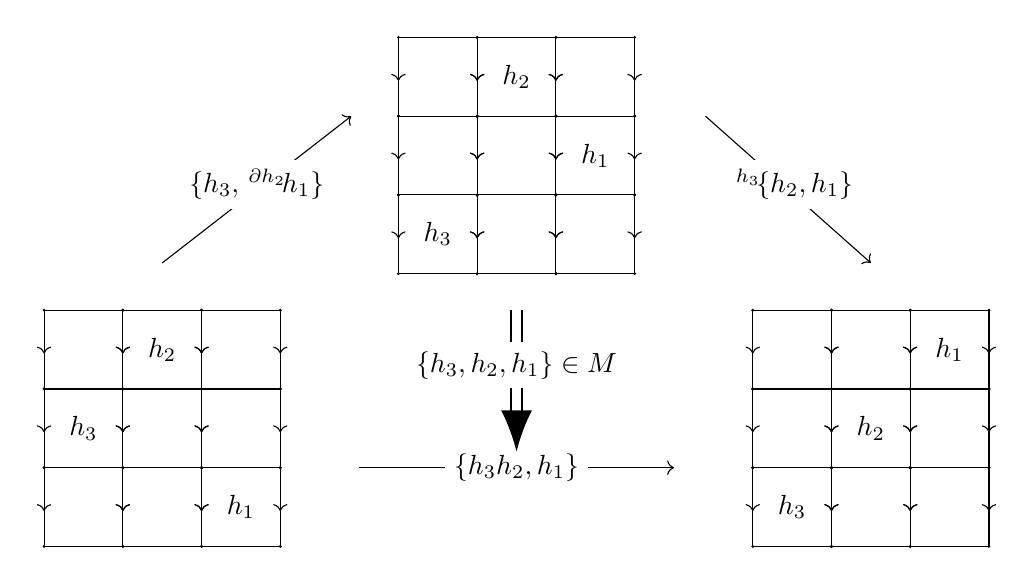
\begin{tikzpicture}[scale=1]
  	\begin{scope}[xshift=0.0cm]
	      \draw (0,0) to node[sloped] {\tikz{\draw[->](0,0)--(0.1,0);}} (0,-1);
	      \draw (1,0) to node[sloped] {\tikz{\draw[->](0,0)--(0.1,0);}} (1,-1);
	      \draw (0,0) to node[sloped] {\tikz{\draw[-](0,0)--(0.1,0);}} (1,0);
	      \draw (0,-1) to node  {\tikz{\draw[-](0,0)--(0.1,0);}} (1,-1);
	      \node at (1/2,-1/2) {$$};
	      \draw (0,0) to node {\tikz{\draw[-](0,0)--(0.1,0);}}(1,0);
	      \draw (0,-1) to node {\tikz{\draw[-](0,0)--(0.1,0);}} (1,-1);
	      \fill[black] (0,0) circle[radius=0.02];
	      \fill[black] (1,0) circle[radius=0.02];
	      \fill[black] (0,-1) circle[radius=0.02];
	      \fill[black] (1,-1) circle[radius=0.02];
	    \begin{scope}[xshift=1.0cm]
	      \draw (0,0) to node[sloped] {\tikz{\draw[->](0,0)--(0.1,0);}} (0,-1);
	      \draw (1,0) to node[sloped] {\tikz{\draw[->](0,0)--(0.1,0);}} (1,-1);
	      \draw (0,0) to node[sloped] {\tikz{\draw[-](0,0)--(0.1,0);}} (1,0);
	      \draw (0,-1) to node  {\tikz{\draw[-](0,0)--(0.1,0);}} (1,-1);
	      \node at (1/2,-1/2) {$h_2$};
	      \draw (0,0) to node {\tikz{\draw[-](0,0)--(0.1,0);}} (1,0);
	      \draw (0,-1) to node {\tikz{\draw[-](0,0)--(0.1,0);}} (1,-1);
	      \fill[black] (0,0) circle[radius=0.02];
	      \fill[black] (1,0) circle[radius=0.02];
	      \fill[black] (0,-1) circle[radius=0.02];
	      \fill[black] (1,-1) circle[radius=0.02];
	    \end{scope}
	    	 \begin{scope}[xshift=2.0cm]
	      \draw (0,0) to node[sloped] {\tikz{\draw[->](0,0)--(0.1,0);}} (0,-1);
	      \draw (1,0) to node[sloped] {\tikz{\draw[->](0,0)--(0.1,0);}} (1,-1);
	      \draw (0,0) to node[sloped] {\tikz{\draw[-](0,0)--(0.1,0);}} (1,0);
	      \draw (0,-1) to node  {\tikz{\draw[-](0,0)--(0.1,0);}} (1,-1);
	      \node at (1/2,-1/2) {$$};
	      \draw (0,0) to node {\tikz{\draw[-](0,0)--(0.1,0);}} (1,0);
	      \draw (0,-1) to node {\tikz{\draw[-](0,0)--(0.1,0);}} (1,-1);
	      \fill[black] (0,0) circle[radius=0.02];
	      \fill[black] (1,0) circle[radius=0.02];
	      \fill[black] (0,-1) circle[radius=0.02];
	      \fill[black] (1,-1) circle[radius=0.02];
	    \end{scope}
	        \begin{scope}[xshift=0.0cm, yshift = -1.0cm]
	      \draw (0,0) to node[sloped] {\tikz{\draw[->](0,0)--(0.1,0);}} (0,-1);
	      \draw (1,0) to node[sloped] {\tikz{\draw[->](0,0)--(0.1,0);}} (1,-1);
	      \draw (0,0) to node[sloped] {\tikz{\draw[-](0,0)--(0.1,0);}} (1,0);
	      \draw (0,-1) to node  {\tikz{\draw[-](0,0)--(0.1,0);}} (1,-1);
	      \node at (1/2,-1/2) {$h_3$};
	      \draw (0,0) to node {\tikz{\draw[-](0,0)--(0.1,0);}} (1,0);
	      \draw (0,-1) to node {\tikz{\draw[-](0,0)--(0.1,0);}} (1,-1);
	      \fill[black] (0,0) circle[radius=0.02];
	      \fill[black] (1,0) circle[radius=0.02];
	      \fill[black] (0,-1) circle[radius=0.02];
	      \fill[black] (1,-1) circle[radius=0.02];
	    \end{scope}
	    \begin{scope}[xshift=1.0cm, yshift = -1.0cm]
	      \draw (0,0) to node[sloped] {\tikz{\draw[->](0,0)--(0.1,0);}} (0,-1);
	      \draw (1,0) to node[sloped] {\tikz{\draw[->](0,0)--(0.1,0);}} (1,-1);
	      \draw (0,0) to node[sloped] {\tikz{\draw[-](0,0)--(0.1,0);}} (1,0);
	      \draw (0,-1) to node  {\tikz{\draw[-](0,0)--(0.1,0);}} (1,-1);
	      \node at (1/2,-1/2) {$$};
	      \draw (0,0) to node {\tikz{\draw[-](0,0)--(0.1,0);}} (1,0);
	      \draw (0,-1) to node {\tikz{\draw[-](0,0)--(0.1,0);}} (1,-1);
	      \fill[black] (0,0) circle[radius=0.02];
	      \fill[black] (1,0) circle[radius=0.02];
	      \fill[black] (0,-1) circle[radius=0.02];
	      \fill[black] (1,-1) circle[radius=0.02];
	    \end{scope}
	     \begin{scope}[xshift=2.0cm, yshift = -1.0cm]
	      \draw (0,0) to node[sloped] {\tikz{\draw[->](0,0)--(0.1,0);}} (0,-1);
	      \draw (1,0) to node[sloped] {\tikz{\draw[->](0,0)--(0.1,0);}} (1,-1);
	      \draw (0,0) to node[sloped] {\tikz{\draw[-](0,0)--(0.1,0);}} (1,0);
	      \draw (0,-1) to node  {\tikz{\draw[-](0,0)--(0.1,0);}} (1,-1);
	      \node at (1/2,-1/2) {$$};
	      \draw (0,0) to node {\tikz{\draw[-](0,0)--(0.1,0);}} (1,0);
	      \draw (0,-1) to node {\tikz{\draw[-](0,0)--(0.1,0);}} (1,-1);
	      \fill[black] (0,0) circle[radius=0.02];
	      \fill[black] (1,0) circle[radius=0.02];
	      \fill[black] (0,-1) circle[radius=0.02];
	      \fill[black] (1,-1) circle[radius=0.02];
	    \end{scope}
	     \begin{scope}[xshift=0.0cm, yshift = -2.0cm]
	      \draw (0,0) to node[sloped] {\tikz{\draw[->](0,0)--(0.1,0);}} (0,-1);
	      \draw (1,0) to node[sloped] {\tikz{\draw[->](0,0)--(0.1,0);}} (1,-1);
	      \draw (0,0) to node[sloped] {\tikz{\draw[-](0,0)--(0.1,0);}} (1,0);
	      \draw (0,-1) to node  {\tikz{\draw[-](0,0)--(0.1,0);}} (1,-1);
	      \node at (1/2,-1/2) {$$};
	      \draw (0,0) to node {\tikz{\draw[-](0,0)--(0.1,0);}} (1,0);
	      \draw (0,-1) to node {\tikz{\draw[-](0,0)--(0.1,0);}} (1,-1);
	      \fill[black] (0,0) circle[radius=0.02];
	      \fill[black] (1,0) circle[radius=0.02];
	      \fill[black] (0,-1) circle[radius=0.02];
	      \fill[black] (1,-1) circle[radius=0.02];
	    \end{scope}
	    \begin{scope}[xshift=1.0cm, yshift = -2.0cm]
	      \draw (0,0) to node[sloped] {\tikz{\draw[->](0,0)--(0.1,0);}} (0,-1);
	      \draw (1,0) to node[sloped] {\tikz{\draw[->](0,0)--(0.1,0);}} (1,-1);
	      \draw (0,0) to node[sloped] {\tikz{\draw[-](0,0)--(0.1,0);}} (1,0);
	      \draw (0,-1) to node  {\tikz{\draw[-](0,0)--(0.1,0);}} (1,-1);
	      \node at (1/2,-1/2) {$$};
	      \draw (0,0) to node {\tikz{\draw[-](0,0)--(0.1,0);}}(1,0);
	      \draw (0,-1) to node {\tikz{\draw[-](0,0)--(0.1,0);}} (1,-1);
	      \fill[black] (0,0) circle[radius=0.02];
	      \fill[black] (1,0) circle[radius=0.02];
	      \fill[black] (0,-1) circle[radius=0.02];
	      \fill[black] (1,-1) circle[radius=0.02];
	    \end{scope}
	     \begin{scope}[xshift=2.0cm, yshift = -2.0cm]
	      \draw (0,0) to node[sloped] {\tikz{\draw[->](0,0)--(0.1,0);}} (0,-1);
	      \draw (1,0) to node[sloped] {\tikz{\draw[->](0,0)--(0.1,0);}} (1,-1);
	      \draw (0,0) to node[sloped] {\tikz{\draw[-](0,0)--(0.1,0);}} (1,0);
	      \draw (0,-1) to node  {\tikz{\draw[-](0,0)--(0.1,0);}} (1,-1);
	      \node at (1/2,-1/2) {$h_1$};
	      \draw (0,0) to node {\tikz{\draw[-](0,0)--(0.1,0);}}(1,0);
	      \draw (0,-1) to node {\tikz{\draw[-](0,0)--(0.1,0);}} (1,-1);
	      \fill[black] (0,0) circle[radius=0.02];
	      \fill[black] (1,0) circle[radius=0.02];
	      \fill[black] (0,-1) circle[radius=0.02];
	      \fill[black] (1,-1) circle[radius=0.02];
	    \end{scope}
    \end{scope}
    \begin{scope}[xshift=4.5cm, yshift = 2*1.732cm]
	      \draw (0,0) to node[sloped] {\tikz{\draw[->](0,0)--(0.1,0);}} (0,-1);
	      \draw (1,0) to node[sloped] {\tikz{\draw[->](0,0)--(0.1,0);}} (1,-1);
	      \draw (0,0) to node[sloped] {\tikz{\draw[-](0,0)--(0.1,0);}} (1,0);
	      \draw (0,-1) to node  {\tikz{\draw[-](0,0)--(0.1,0);}} (1,-1);
	      \node at (1/2,-1/2) {$$};
	      \draw (0,0) to node {\tikz{\draw[-](0,0)--(0.1,0);}}(1,0);
	      \draw (0,-1) to node {\tikz{\draw[-](0,0)--(0.1,0);}} (1,-1);
	      \fill[black] (0,0) circle[radius=0.02];
	      \fill[black] (1,0) circle[radius=0.02];
	      \fill[black] (0,-1) circle[radius=0.02];
	      \fill[black] (1,-1) circle[radius=0.02];
	    \begin{scope}[xshift=1.0cm]
	      \draw (0,0) to node[sloped] {\tikz{\draw[->](0,0)--(0.1,0);}} (0,-1);
	      \draw (1,0) to node[sloped] {\tikz{\draw[->](0,0)--(0.1,0);}} (1,-1);
	      \draw (0,0) to node[sloped] {\tikz{\draw[-](0,0)--(0.1,0);}} (1,0);
	      \draw (0,-1) to node  {\tikz{\draw[-](0,0)--(0.1,0);}} (1,-1);
	      \node at (1/2,-1/2) {$h_2$};
	      \draw (0,0) to node {\tikz{\draw[-](0,0)--(0.1,0);}} (1,0);
	      \draw (0,-1) to node {\tikz{\draw[-](0,0)--(0.1,0);}} (1,-1);
	      \fill[black] (0,0) circle[radius=0.02];
	      \fill[black] (1,0) circle[radius=0.02];
	      \fill[black] (0,-1) circle[radius=0.02];
	      \fill[black] (1,-1) circle[radius=0.02];
	    \end{scope}
	    	 \begin{scope}[xshift=2.0cm]
	      \draw (0,0) to node[sloped] {\tikz{\draw[->](0,0)--(0.1,0);}} (0,-1);
	      \draw (1,0) to node[sloped] {\tikz{\draw[->](0,0)--(0.1,0);}} (1,-1);
	      \draw (0,0) to node[sloped] {\tikz{\draw[-](0,0)--(0.1,0);}} (1,0);
	      \draw (0,-1) to node  {\tikz{\draw[-](0,0)--(0.1,0);}} (1,-1);
	      \node at (1/2,-1/2) {$$};
	      \draw (0,0) to node {\tikz{\draw[-](0,0)--(0.1,0);}} (1,0);
	      \draw (0,-1) to node {\tikz{\draw[-](0,0)--(0.1,0);}} (1,-1);
	      \fill[black] (0,0) circle[radius=0.02];
	      \fill[black] (1,0) circle[radius=0.02];
	      \fill[black] (0,-1) circle[radius=0.02];
	      \fill[black] (1,-1) circle[radius=0.02];
	    \end{scope}
	        \begin{scope}[xshift=0.0cm, yshift = -1.0cm]
	      \draw (0,0) to node[sloped] {\tikz{\draw[->](0,0)--(0.1,0);}} (0,-1);
	      \draw (1,0) to node[sloped] {\tikz{\draw[->](0,0)--(0.1,0);}} (1,-1);
	      \draw (0,0) to node[sloped] {\tikz{\draw[-](0,0)--(0.1,0);}} (1,0);
	      \draw (0,-1) to node  {\tikz{\draw[-](0,0)--(0.1,0);}} (1,-1);
	      \node at (1/2,-1/2) {$$};
	      \draw (0,0) to node {\tikz{\draw[-](0,0)--(0.1,0);}} (1,0);
	      \draw (0,-1) to node {\tikz{\draw[-](0,0)--(0.1,0);}} (1,-1);
	      \fill[black] (0,0) circle[radius=0.02];
	      \fill[black] (1,0) circle[radius=0.02];
	      \fill[black] (0,-1) circle[radius=0.02];
	      \fill[black] (1,-1) circle[radius=0.02];
	    \end{scope}
	    \begin{scope}[xshift=1.0cm, yshift = -1.0cm]
	      \draw (0,0) to node[sloped] {\tikz{\draw[->](0,0)--(0.1,0);}} (0,-1);
	      \draw (1,0) to node[sloped] {\tikz{\draw[->](0,0)--(0.1,0);}} (1,-1);
	      \draw (0,0) to node[sloped] {\tikz{\draw[-](0,0)--(0.1,0);}} (1,0);
	      \draw (0,-1) to node  {\tikz{\draw[-](0,0)--(0.1,0);}} (1,-1);
	      \node at (1/2,-1/2) {$$};
	      \draw (0,0) to node {\tikz{\draw[-](0,0)--(0.1,0);}} (1,0);
	      \draw (0,-1) to node {\tikz{\draw[-](0,0)--(0.1,0);}} (1,-1);
	      \fill[black] (0,0) circle[radius=0.02];
	      \fill[black] (1,0) circle[radius=0.02];
	      \fill[black] (0,-1) circle[radius=0.02];
	      \fill[black] (1,-1) circle[radius=0.02];
	    \end{scope}
	     \begin{scope}[xshift=2.0cm, yshift = -1.0cm]
	      \draw (0,0) to node[sloped] {\tikz{\draw[->](0,0)--(0.1,0);}} (0,-1);
	      \draw (1,0) to node[sloped] {\tikz{\draw[->](0,0)--(0.1,0);}} (1,-1);
	      \draw (0,0) to node[sloped] {\tikz{\draw[-](0,0)--(0.1,0);}} (1,0);
	      \draw (0,-1) to node  {\tikz{\draw[-](0,0)--(0.1,0);}} (1,-1);
	      \node at (1/2,-1/2) {$h_1$};
	      \draw (0,0) to node {\tikz{\draw[-](0,0)--(0.1,0);}} (1,0);
	      \draw (0,-1) to node {\tikz{\draw[-](0,0)--(0.1,0);}} (1,-1);
	      \fill[black] (0,0) circle[radius=0.02];
	      \fill[black] (1,0) circle[radius=0.02];
	      \fill[black] (0,-1) circle[radius=0.02];
	      \fill[black] (1,-1) circle[radius=0.02];
	    \end{scope}
	     \begin{scope}[xshift=0.0cm, yshift = -2.0cm]
	      \draw (0,0) to node[sloped] {\tikz{\draw[->](0,0)--(0.1,0);}} (0,-1);
	      \draw (1,0) to node[sloped] {\tikz{\draw[->](0,0)--(0.1,0);}} (1,-1);
	      \draw (0,0) to node[sloped] {\tikz{\draw[-](0,0)--(0.1,0);}} (1,0);
	      \draw (0,-1) to node  {\tikz{\draw[-](0,0)--(0.1,0);}} (1,-1);
	      \node at (1/2,-1/2) {$h_3$};
	      \draw (0,0) to node {\tikz{\draw[-](0,0)--(0.1,0);}} (1,0);
	      \draw (0,-1) to node {\tikz{\draw[-](0,0)--(0.1,0);}} (1,-1);
	      \fill[black] (0,0) circle[radius=0.02];
	      \fill[black] (1,0) circle[radius=0.02];
	      \fill[black] (0,-1) circle[radius=0.02];
	      \fill[black] (1,-1) circle[radius=0.02];
	    \end{scope}
	    \begin{scope}[xshift=1.0cm, yshift = -2.0cm]
	      \draw (0,0) to node[sloped] {\tikz{\draw[->](0,0)--(0.1,0);}} (0,-1);
	      \draw (1,0) to node[sloped] {\tikz{\draw[->](0,0)--(0.1,0);}} (1,-1);
	      \draw (0,0) to node[sloped] {\tikz{\draw[-](0,0)--(0.1,0);}} (1,0);
	      \draw (0,-1) to node  {\tikz{\draw[-](0,0)--(0.1,0);}} (1,-1);
	      \node at (1/2,-1/2) {$$};
	      \draw (0,0) to node {\tikz{\draw[-](0,0)--(0.1,0);}}(1,0);
	      \draw (0,-1) to node {\tikz{\draw[-](0,0)--(0.1,0);}} (1,-1);
	      \fill[black] (0,0) circle[radius=0.02];
	      \fill[black] (1,0) circle[radius=0.02];
	      \fill[black] (0,-1) circle[radius=0.02];
	      \fill[black] (1,-1) circle[radius=0.02];
	    \end{scope}
	     \begin{scope}[xshift=2.0cm, yshift = -2.0cm]
	      \draw (0,0) to node[sloped] {\tikz{\draw[->](0,0)--(0.1,0);}} (0,-1);
	      \draw (1,0) to node[sloped] {\tikz{\draw[->](0,0)--(0.1,0);}} (1,-1);
	      \draw (0,0) to node[sloped] {\tikz{\draw[-](0,0)--(0.1,0);}} (1,0);
	      \draw (0,-1) to node  {\tikz{\draw[-](0,0)--(0.1,0);}} (1,-1);
	      \node at (1/2,-1/2) {$$};
	      \draw (0,0) to node {\tikz{\draw[-](0,0)--(0.1,0);}}(1,0);
	      \draw (0,-1) to node {\tikz{\draw[-](0,0)--(0.1,0);}} (1,-1);
	      \fill[black] (0,0) circle[radius=0.02];
	      \fill[black] (1,0) circle[radius=0.02];
	      \fill[black] (0,-1) circle[radius=0.02];
	      \fill[black] (1,-1) circle[radius=0.02];
	    \end{scope}
    \end{scope}
    \begin{scope}[xshift=9.0cm]
	      \draw (0,0) to node[sloped] {\tikz{\draw[->](0,0)--(0.1,0);}} (0,-1);
	      \draw (1,0) to node[sloped] {\tikz{\draw[->](0,0)--(0.1,0);}} (1,-1);
	      \draw (0,0) to node[sloped] {\tikz{\draw[-](0,0)--(0.1,0);}} (1,0);
	      \draw (0,-1) to node  {\tikz{\draw[-](0,0)--(0.1,0);}} (1,-1);
	      \node at (1/2,-1/2) {$$};
	      \draw (0,0) to node {\tikz{\draw[-](0,0)--(0.1,0);}}(1,0);
	      \draw (0,-1) to node {\tikz{\draw[-](0,0)--(0.1,0);}} (1,-1);
	      \fill[black] (0,0) circle[radius=0.02];
	      \fill[black] (1,0) circle[radius=0.02];
	      \fill[black] (0,-1) circle[radius=0.02];
	      \fill[black] (1,-1) circle[radius=0.02];
	    \begin{scope}[xshift=1.0cm]
	      \draw (0,0) to node[sloped] {\tikz{\draw[->](0,0)--(0.1,0);}} (0,-1);
	      \draw (1,0) to node[sloped] {\tikz{\draw[->](0,0)--(0.1,0);}} (1,-1);
	      \draw (0,0) to node[sloped] {\tikz{\draw[-](0,0)--(0.1,0);}} (1,0);
	      \draw (0,-1) to node  {\tikz{\draw[-](0,0)--(0.1,0);}} (1,-1);
	      \node at (1/2,-1/2) {$$};
	      \draw (0,0) to node {\tikz{\draw[-](0,0)--(0.1,0);}} (1,0);
	      \draw (0,-1) to node {\tikz{\draw[-](0,0)--(0.1,0);}} (1,-1);
	      \fill[black] (0,0) circle[radius=0.02];
	      \fill[black] (1,0) circle[radius=0.02];
	      \fill[black] (0,-1) circle[radius=0.02];
	      \fill[black] (1,-1) circle[radius=0.02];
	    \end{scope}
	    	 \begin{scope}[xshift=2.0cm]
	      \draw (0,0) to node[sloped] {\tikz{\draw[->](0,0)--(0.1,0);}} (0,-1);
	      \draw (1,0) to node[sloped] {\tikz{\draw[->](0,0)--(0.1,0);}} (1,-1);
	      \draw (0,0) to node[sloped] {\tikz{\draw[-](0,0)--(0.1,0);}} (1,0);
	      \draw (0,-1) to node  {\tikz{\draw[-](0,0)--(0.1,0);}} (1,-1);
	      \node at (1/2,-1/2) {$h_1$};
	      \draw (0,0) to node {\tikz{\draw[-](0,0)--(0.1,0);}} (1,0);
	      \draw (0,-1) to node {\tikz{\draw[-](0,0)--(0.1,0);}} (1,-1);
	      \fill[black] (0,0) circle[radius=0.02];
	      \fill[black] (1,0) circle[radius=0.02];
	      \fill[black] (0,-1) circle[radius=0.02];
	      \fill[black] (1,-1) circle[radius=0.02];
	    \end{scope}
	        \begin{scope}[xshift=0.0cm, yshift = -1.0cm]
	      \draw (0,0) to node[sloped] {\tikz{\draw[->](0,0)--(0.1,0);}} (0,-1);
	      \draw (1,0) to node[sloped] {\tikz{\draw[->](0,0)--(0.1,0);}} (1,-1);
	      \draw (0,0) to node[sloped] {\tikz{\draw[-](0,0)--(0.1,0);}} (1,0);
	      \draw (0,-1) to node  {\tikz{\draw[-](0,0)--(0.1,0);}} (1,-1);
	      \node at (1/2,-1/2) {$$};
	      \draw (0,0) to node {\tikz{\draw[-](0,0)--(0.1,0);}} (1,0);
	      \draw (0,-1) to node {\tikz{\draw[-](0,0)--(0.1,0);}} (1,-1);
	      \fill[black] (0,0) circle[radius=0.02];
	      \fill[black] (1,0) circle[radius=0.02];
	      \fill[black] (0,-1) circle[radius=0.02];
	      \fill[black] (1,-1) circle[radius=0.02];
	    \end{scope}
	    \begin{scope}[xshift=1.0cm, yshift = -1.0cm]
	      \draw (0,0) to node[sloped] {\tikz{\draw[->](0,0)--(0.1,0);}} (0,-1);
	      \draw (1,0) to node[sloped] {\tikz{\draw[->](0,0)--(0.1,0);}} (1,-1);
	      \draw (0,0) to node[sloped] {\tikz{\draw[-](0,0)--(0.1,0);}} (1,0);
	      \draw (0,-1) to node  {\tikz{\draw[-](0,0)--(0.1,0);}} (1,-1);
	      \node at (1/2,-1/2) {$h_2$};
	      \draw (0,0) to node {\tikz{\draw[-](0,0)--(0.1,0);}} (1,0);
	      \draw (0,-1) to node {\tikz{\draw[-](0,0)--(0.1,0);}} (1,-1);
	      \fill[black] (0,0) circle[radius=0.02];
	      \fill[black] (1,0) circle[radius=0.02];
	      \fill[black] (0,-1) circle[radius=0.02];
	      \fill[black] (1,-1) circle[radius=0.02];
	    \end{scope}
	     \begin{scope}[xshift=2.0cm, yshift = -1.0cm]
	      \draw (0,0) to node[sloped] {\tikz{\draw[->](0,0)--(0.1,0);}} (0,-1);
	      \draw (1,0) to node[sloped] {\tikz{\draw[->](0,0)--(0.1,0);}} (1,-1);
	      \draw (0,0) to node[sloped] {\tikz{\draw[-](0,0)--(0.1,0);}} (1,0);
	      \draw (0,-1) to node  {\tikz{\draw[-](0,0)--(0.1,0);}} (1,-1);
	      \node at (1/2,-1/2) {$$};
	      \draw (0,0) to node {\tikz{\draw[-](0,0)--(0.1,0);}} (1,0);
	      \draw (0,-1) to node {\tikz{\draw[-](0,0)--(0.1,0);}} (1,-1);
	      \fill[black] (0,0) circle[radius=0.02];
	      \fill[black] (1,0) circle[radius=0.02];
	      \fill[black] (0,-1) circle[radius=0.02];
	      \fill[black] (1,-1) circle[radius=0.02];
	    \end{scope}
	     \begin{scope}[xshift=0.0cm, yshift = -2.0cm]
	      \draw (0,0) to node[sloped] {\tikz{\draw[->](0,0)--(0.1,0);}} (0,-1);
	      \draw (1,0) to node[sloped] {\tikz{\draw[->](0,0)--(0.1,0);}} (1,-1);
	      \draw (0,0) to node[sloped] {\tikz{\draw[-](0,0)--(0.1,0);}} (1,0);
	      \draw (0,-1) to node  {\tikz{\draw[-](0,0)--(0.1,0);}} (1,-1);
	      \node at (1/2,-1/2) {$h_3$};
	      \draw (0,0) to node {\tikz{\draw[-](0,0)--(0.1,0);}} (1,0);
	      \draw (0,-1) to node {\tikz{\draw[-](0,0)--(0.1,0);}} (1,-1);
	      \fill[black] (0,0) circle[radius=0.02];
	      \fill[black] (1,0) circle[radius=0.02];
	      \fill[black] (0,-1) circle[radius=0.02];
	      \fill[black] (1,-1) circle[radius=0.02];
	    \end{scope}
	    \begin{scope}[xshift=1.0cm, yshift = -2.0cm]
	      \draw (0,0) to node[sloped] {\tikz{\draw[->](0,0)--(0.1,0);}} (0,-1);
	      \draw (1,0) to node[sloped] {\tikz{\draw[->](0,0)--(0.1,0);}} (1,-1);
	      \draw (0,0) to node[sloped] {\tikz{\draw[-](0,0)--(0.1,0);}} (1,0);
	      \draw (0,-1) to node  {\tikz{\draw[-](0,0)--(0.1,0);}} (1,-1);
	      \node at (1/2,-1/2) {$$};
	      \draw (0,0) to node {\tikz{\draw[-](0,0)--(0.1,0);}}(1,0);
	      \draw (0,-1) to node {\tikz{\draw[-](0,0)--(0.1,0);}} (1,-1);
	      \fill[black] (0,0) circle[radius=0.02];
	      \fill[black] (1,0) circle[radius=0.02];
	      \fill[black] (0,-1) circle[radius=0.02];
	      \fill[black] (1,-1) circle[radius=0.02];
	    \end{scope}
	     \begin{scope}[xshift=2.0cm, yshift = -2.0cm]
	      \draw (0,0) to node[sloped] {\tikz{\draw[->](0,0)--(0.1,0);}} (0,-1);
	      \draw (1,0) to node[sloped] {\tikz{\draw[->](0,0)--(0.1,0);}} (1,-1);
	      \draw (0,0) to node[sloped] {\tikz{\draw[-](0,0)--(0.1,0);}} (1,0);
	      \draw (0,-1) to node  {\tikz{\draw[-](0,0)--(0.1,0);}} (1,-1);
	      \node at (1/2,-1/2) {$$};
	      \draw (0,0) to node {\tikz{\draw[-](0,0)--(0.1,0);}}(1,0);
	      \draw (0,-1) to node {\tikz{\draw[-](0,0)--(0.1,0);}} (1,-1);
	      \fill[black] (0,0) circle[radius=0.02];
	      \fill[black] (1,0) circle[radius=0.02];
	      \fill[black] (0,-1) circle[radius=0.02];
	      \fill[black] (1,-1) circle[radius=0.02];
	    \end{scope}
    \end{scope}
     \draw[->] (4,-2) to (8,-2);
      \node at (6,-2) [fill=white]{$\{h_3 h_2, h_1\}$};
       \draw[->] (1.5 , 0.1+1/2) to (4.4-1/2,-1+ 2*1.732);
      \node at (2.7,1.6) [fill=white]{$\{h_3, \act{\del h_2}h_1 \}$};
       \draw[->](3+4.4+1,-1+ 2*1.732) to (10.5, 0.6);
      \node at (9.5,1.6)  [fill=white]{$\act{h_3}\{h_2, h_1\}$};
      \draw [line width=1pt, double distance=3pt, arrows = {-Latex[length=0pt 3 0]}] (6,0) -- (6,-1.8);
      \node at (6, -0.7)  [fill=white]{$\{h_3,h_2, h_1\}\in M$};
  \end{tikzpicture}
\end{center}
\caption{Figure of left-homanian}
\label{d:lhmn}
\end{figure}

Similarly, the right-homannian is a twisted version of Property~\ref{rpl} of a 2-crossed module, as shown in Figure~\ref{d:rhmn}.

\begin{figure}
\begin{center}
  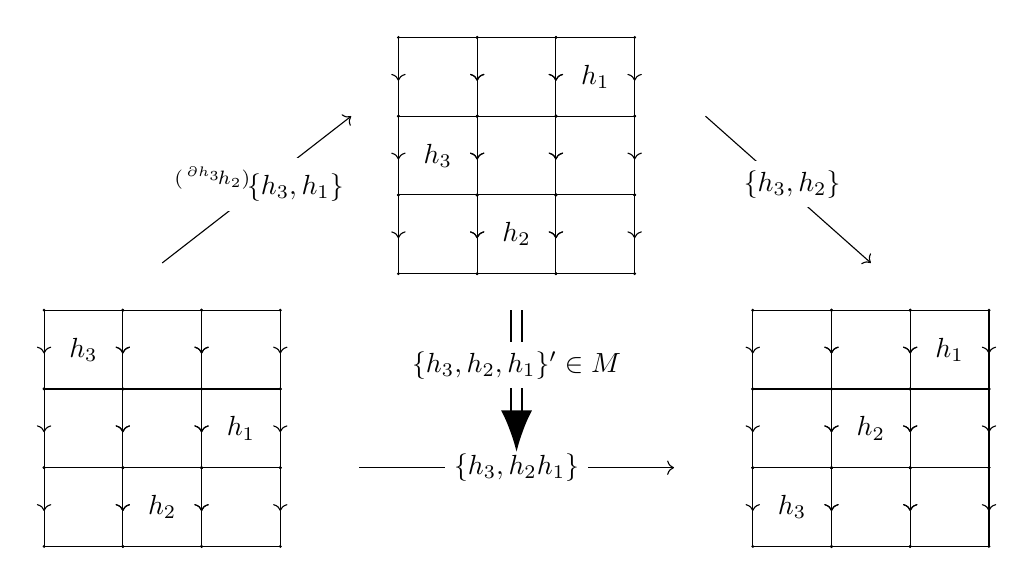
\begin{tikzpicture}[scale=1]
  	\begin{scope}[xshift=0.0cm]
	      \draw (0,0) to node[sloped] {\tikz{\draw[->](0,0)--(0.1,0);}} (0,-1);
	      \draw (1,0) to node[sloped] {\tikz{\draw[->](0,0)--(0.1,0);}} (1,-1);
	      \draw (0,0) to node[sloped] {\tikz{\draw[-](0,0)--(0.1,0);}} (1,0);
	      \draw (0,-1) to node  {\tikz{\draw[-](0,0)--(0.1,0);}} (1,-1);
	      \node at (1/2,-1/2) {$h_3$};
	      \draw (0,0) to node {\tikz{\draw[-](0,0)--(0.1,0);}}(1,0);
	      \draw (0,-1) to node {\tikz{\draw[-](0,0)--(0.1,0);}} (1,-1);
	      \fill[black] (0,0) circle[radius=0.02];
	      \fill[black] (1,0) circle[radius=0.02];
	      \fill[black] (0,-1) circle[radius=0.02];
	      \fill[black] (1,-1) circle[radius=0.02];
	    \begin{scope}[xshift=1.0cm]
	      \draw (0,0) to node[sloped] {\tikz{\draw[->](0,0)--(0.1,0);}} (0,-1);
	      \draw (1,0) to node[sloped] {\tikz{\draw[->](0,0)--(0.1,0);}} (1,-1);
	      \draw (0,0) to node[sloped] {\tikz{\draw[-](0,0)--(0.1,0);}} (1,0);
	      \draw (0,-1) to node  {\tikz{\draw[-](0,0)--(0.1,0);}} (1,-1);
	      \node at (1/2,-1/2) {$$};
	      \draw (0,0) to node {\tikz{\draw[-](0,0)--(0.1,0);}} (1,0);
	      \draw (0,-1) to node {\tikz{\draw[-](0,0)--(0.1,0);}} (1,-1);
	      \fill[black] (0,0) circle[radius=0.02];
	      \fill[black] (1,0) circle[radius=0.02];
	      \fill[black] (0,-1) circle[radius=0.02];
	      \fill[black] (1,-1) circle[radius=0.02];
	    \end{scope}
	    	 \begin{scope}[xshift=2.0cm]
	      \draw (0,0) to node[sloped] {\tikz{\draw[->](0,0)--(0.1,0);}} (0,-1);
	      \draw (1,0) to node[sloped] {\tikz{\draw[->](0,0)--(0.1,0);}} (1,-1);
	      \draw (0,0) to node[sloped] {\tikz{\draw[-](0,0)--(0.1,0);}} (1,0);
	      \draw (0,-1) to node  {\tikz{\draw[-](0,0)--(0.1,0);}} (1,-1);
	      \node at (1/2,-1/2) {$$};
	      \draw (0,0) to node {\tikz{\draw[-](0,0)--(0.1,0);}} (1,0);
	      \draw (0,-1) to node {\tikz{\draw[-](0,0)--(0.1,0);}} (1,-1);
	      \fill[black] (0,0) circle[radius=0.02];
	      \fill[black] (1,0) circle[radius=0.02];
	      \fill[black] (0,-1) circle[radius=0.02];
	      \fill[black] (1,-1) circle[radius=0.02];
	    \end{scope}
	        \begin{scope}[xshift=0.0cm, yshift = -1.0cm]
	      \draw (0,0) to node[sloped] {\tikz{\draw[->](0,0)--(0.1,0);}} (0,-1);
	      \draw (1,0) to node[sloped] {\tikz{\draw[->](0,0)--(0.1,0);}} (1,-1);
	      \draw (0,0) to node[sloped] {\tikz{\draw[-](0,0)--(0.1,0);}} (1,0);
	      \draw (0,-1) to node  {\tikz{\draw[-](0,0)--(0.1,0);}} (1,-1);
	      \node at (1/2,-1/2) {$$};
	      \draw (0,0) to node {\tikz{\draw[-](0,0)--(0.1,0);}} (1,0);
	      \draw (0,-1) to node {\tikz{\draw[-](0,0)--(0.1,0);}} (1,-1);
	      \fill[black] (0,0) circle[radius=0.02];
	      \fill[black] (1,0) circle[radius=0.02];
	      \fill[black] (0,-1) circle[radius=0.02];
	      \fill[black] (1,-1) circle[radius=0.02];
	    \end{scope}
	    \begin{scope}[xshift=1.0cm, yshift = -1.0cm]
	      \draw (0,0) to node[sloped] {\tikz{\draw[->](0,0)--(0.1,0);}} (0,-1);
	      \draw (1,0) to node[sloped] {\tikz{\draw[->](0,0)--(0.1,0);}} (1,-1);
	      \draw (0,0) to node[sloped] {\tikz{\draw[-](0,0)--(0.1,0);}} (1,0);
	      \draw (0,-1) to node  {\tikz{\draw[-](0,0)--(0.1,0);}} (1,-1);
	      \node at (1/2,-1/2) {$$};
	      \draw (0,0) to node {\tikz{\draw[-](0,0)--(0.1,0);}} (1,0);
	      \draw (0,-1) to node {\tikz{\draw[-](0,0)--(0.1,0);}} (1,-1);
	      \fill[black] (0,0) circle[radius=0.02];
	      \fill[black] (1,0) circle[radius=0.02];
	      \fill[black] (0,-1) circle[radius=0.02];
	      \fill[black] (1,-1) circle[radius=0.02];
	    \end{scope}
	     \begin{scope}[xshift=2.0cm, yshift = -1.0cm]
	      \draw (0,0) to node[sloped] {\tikz{\draw[->](0,0)--(0.1,0);}} (0,-1);
	      \draw (1,0) to node[sloped] {\tikz{\draw[->](0,0)--(0.1,0);}} (1,-1);
	      \draw (0,0) to node[sloped] {\tikz{\draw[-](0,0)--(0.1,0);}} (1,0);
	      \draw (0,-1) to node  {\tikz{\draw[-](0,0)--(0.1,0);}} (1,-1);
	      \node at (1/2,-1/2) {$h_1$};
	      \draw (0,0) to node {\tikz{\draw[-](0,0)--(0.1,0);}} (1,0);
	      \draw (0,-1) to node {\tikz{\draw[-](0,0)--(0.1,0);}} (1,-1);
	      \fill[black] (0,0) circle[radius=0.02];
	      \fill[black] (1,0) circle[radius=0.02];
	      \fill[black] (0,-1) circle[radius=0.02];
	      \fill[black] (1,-1) circle[radius=0.02];
	    \end{scope}
	     \begin{scope}[xshift=0.0cm, yshift = -2.0cm]
	      \draw (0,0) to node[sloped] {\tikz{\draw[->](0,0)--(0.1,0);}} (0,-1);
	      \draw (1,0) to node[sloped] {\tikz{\draw[->](0,0)--(0.1,0);}} (1,-1);
	      \draw (0,0) to node[sloped] {\tikz{\draw[-](0,0)--(0.1,0);}} (1,0);
	      \draw (0,-1) to node  {\tikz{\draw[-](0,0)--(0.1,0);}} (1,-1);
	      \node at (1/2,-1/2) {$$};
	      \draw (0,0) to node {\tikz{\draw[-](0,0)--(0.1,0);}} (1,0);
	      \draw (0,-1) to node {\tikz{\draw[-](0,0)--(0.1,0);}} (1,-1);
	      \fill[black] (0,0) circle[radius=0.02];
	      \fill[black] (1,0) circle[radius=0.02];
	      \fill[black] (0,-1) circle[radius=0.02];
	      \fill[black] (1,-1) circle[radius=0.02];
	    \end{scope}
	    \begin{scope}[xshift=1.0cm, yshift = -2.0cm]
	      \draw (0,0) to node[sloped] {\tikz{\draw[->](0,0)--(0.1,0);}} (0,-1);
	      \draw (1,0) to node[sloped] {\tikz{\draw[->](0,0)--(0.1,0);}} (1,-1);
	      \draw (0,0) to node[sloped] {\tikz{\draw[-](0,0)--(0.1,0);}} (1,0);
	      \draw (0,-1) to node  {\tikz{\draw[-](0,0)--(0.1,0);}} (1,-1);
	      \node at (1/2,-1/2) {$h_2$};
	      \draw (0,0) to node {\tikz{\draw[-](0,0)--(0.1,0);}}(1,0);
	      \draw (0,-1) to node {\tikz{\draw[-](0,0)--(0.1,0);}} (1,-1);
	      \fill[black] (0,0) circle[radius=0.02];
	      \fill[black] (1,0) circle[radius=0.02];
	      \fill[black] (0,-1) circle[radius=0.02];
	      \fill[black] (1,-1) circle[radius=0.02];
	    \end{scope}
	     \begin{scope}[xshift=2.0cm, yshift = -2.0cm]
	      \draw (0,0) to node[sloped] {\tikz{\draw[->](0,0)--(0.1,0);}} (0,-1);
	      \draw (1,0) to node[sloped] {\tikz{\draw[->](0,0)--(0.1,0);}} (1,-1);
	      \draw (0,0) to node[sloped] {\tikz{\draw[-](0,0)--(0.1,0);}} (1,0);
	      \draw (0,-1) to node  {\tikz{\draw[-](0,0)--(0.1,0);}} (1,-1);
	      \node at (1/2,-1/2) {$$};
	      \draw (0,0) to node {\tikz{\draw[-](0,0)--(0.1,0);}}(1,0);
	      \draw (0,-1) to node {\tikz{\draw[-](0,0)--(0.1,0);}} (1,-1);
	      \fill[black] (0,0) circle[radius=0.02];
	      \fill[black] (1,0) circle[radius=0.02];
	      \fill[black] (0,-1) circle[radius=0.02];
	      \fill[black] (1,-1) circle[radius=0.02];
	    \end{scope}
    \end{scope}
    \begin{scope}[xshift=4.5cm, yshift = 2*1.732cm]
	      \draw (0,0) to node[sloped] {\tikz{\draw[->](0,0)--(0.1,0);}} (0,-1);
	      \draw (1,0) to node[sloped] {\tikz{\draw[->](0,0)--(0.1,0);}} (1,-1);
	      \draw (0,0) to node[sloped] {\tikz{\draw[-](0,0)--(0.1,0);}} (1,0);
	      \draw (0,-1) to node  {\tikz{\draw[-](0,0)--(0.1,0);}} (1,-1);
	      \node at (1/2,-1/2) {$$};
	      \draw (0,0) to node {\tikz{\draw[-](0,0)--(0.1,0);}}(1,0);
	      \draw (0,-1) to node {\tikz{\draw[-](0,0)--(0.1,0);}} (1,-1);
	      \fill[black] (0,0) circle[radius=0.02];
	      \fill[black] (1,0) circle[radius=0.02];
	      \fill[black] (0,-1) circle[radius=0.02];
	      \fill[black] (1,-1) circle[radius=0.02];
	    \begin{scope}[xshift=1.0cm]
	      \draw (0,0) to node[sloped] {\tikz{\draw[->](0,0)--(0.1,0);}} (0,-1);
	      \draw (1,0) to node[sloped] {\tikz{\draw[->](0,0)--(0.1,0);}} (1,-1);
	      \draw (0,0) to node[sloped] {\tikz{\draw[-](0,0)--(0.1,0);}} (1,0);
	      \draw (0,-1) to node  {\tikz{\draw[-](0,0)--(0.1,0);}} (1,-1);
	      \node at (1/2,-1/2) {$$};
	      \draw (0,0) to node {\tikz{\draw[-](0,0)--(0.1,0);}} (1,0);
	      \draw (0,-1) to node {\tikz{\draw[-](0,0)--(0.1,0);}} (1,-1);
	      \fill[black] (0,0) circle[radius=0.02];
	      \fill[black] (1,0) circle[radius=0.02];
	      \fill[black] (0,-1) circle[radius=0.02];
	      \fill[black] (1,-1) circle[radius=0.02];
	    \end{scope}
	    	 \begin{scope}[xshift=2.0cm]
	      \draw (0,0) to node[sloped] {\tikz{\draw[->](0,0)--(0.1,0);}} (0,-1);
	      \draw (1,0) to node[sloped] {\tikz{\draw[->](0,0)--(0.1,0);}} (1,-1);
	      \draw (0,0) to node[sloped] {\tikz{\draw[-](0,0)--(0.1,0);}} (1,0);
	      \draw (0,-1) to node  {\tikz{\draw[-](0,0)--(0.1,0);}} (1,-1);
	      \node at (1/2,-1/2) {$h_1$};
	      \draw (0,0) to node {\tikz{\draw[-](0,0)--(0.1,0);}} (1,0);
	      \draw (0,-1) to node {\tikz{\draw[-](0,0)--(0.1,0);}} (1,-1);
	      \fill[black] (0,0) circle[radius=0.02];
	      \fill[black] (1,0) circle[radius=0.02];
	      \fill[black] (0,-1) circle[radius=0.02];
	      \fill[black] (1,-1) circle[radius=0.02];
	    \end{scope}
	        \begin{scope}[xshift=0.0cm, yshift = -1.0cm]
	      \draw (0,0) to node[sloped] {\tikz{\draw[->](0,0)--(0.1,0);}} (0,-1);
	      \draw (1,0) to node[sloped] {\tikz{\draw[->](0,0)--(0.1,0);}} (1,-1);
	      \draw (0,0) to node[sloped] {\tikz{\draw[-](0,0)--(0.1,0);}} (1,0);
	      \draw (0,-1) to node  {\tikz{\draw[-](0,0)--(0.1,0);}} (1,-1);
	      \node at (1/2,-1/2) {$h_3$};
	      \draw (0,0) to node {\tikz{\draw[-](0,0)--(0.1,0);}} (1,0);
	      \draw (0,-1) to node {\tikz{\draw[-](0,0)--(0.1,0);}} (1,-1);
	      \fill[black] (0,0) circle[radius=0.02];
	      \fill[black] (1,0) circle[radius=0.02];
	      \fill[black] (0,-1) circle[radius=0.02];
	      \fill[black] (1,-1) circle[radius=0.02];
	    \end{scope}
	    \begin{scope}[xshift=1.0cm, yshift = -1.0cm]
	      \draw (0,0) to node[sloped] {\tikz{\draw[->](0,0)--(0.1,0);}} (0,-1);
	      \draw (1,0) to node[sloped] {\tikz{\draw[->](0,0)--(0.1,0);}} (1,-1);
	      \draw (0,0) to node[sloped] {\tikz{\draw[-](0,0)--(0.1,0);}} (1,0);
	      \draw (0,-1) to node  {\tikz{\draw[-](0,0)--(0.1,0);}} (1,-1);
	      \node at (1/2,-1/2) {$$};
	      \draw (0,0) to node {\tikz{\draw[-](0,0)--(0.1,0);}} (1,0);
	      \draw (0,-1) to node {\tikz{\draw[-](0,0)--(0.1,0);}} (1,-1);
	      \fill[black] (0,0) circle[radius=0.02];
	      \fill[black] (1,0) circle[radius=0.02];
	      \fill[black] (0,-1) circle[radius=0.02];
	      \fill[black] (1,-1) circle[radius=0.02];
	    \end{scope}
	     \begin{scope}[xshift=2.0cm, yshift = -1.0cm]
	      \draw (0,0) to node[sloped] {\tikz{\draw[->](0,0)--(0.1,0);}} (0,-1);
	      \draw (1,0) to node[sloped] {\tikz{\draw[->](0,0)--(0.1,0);}} (1,-1);
	      \draw (0,0) to node[sloped] {\tikz{\draw[-](0,0)--(0.1,0);}} (1,0);
	      \draw (0,-1) to node  {\tikz{\draw[-](0,0)--(0.1,0);}} (1,-1);
	      \node at (1/2,-1/2) {$$};
	      \draw (0,0) to node {\tikz{\draw[-](0,0)--(0.1,0);}} (1,0);
	      \draw (0,-1) to node {\tikz{\draw[-](0,0)--(0.1,0);}} (1,-1);
	      \fill[black] (0,0) circle[radius=0.02];
	      \fill[black] (1,0) circle[radius=0.02];
	      \fill[black] (0,-1) circle[radius=0.02];
	      \fill[black] (1,-1) circle[radius=0.02];
	    \end{scope}
	     \begin{scope}[xshift=0.0cm, yshift = -2.0cm]
	      \draw (0,0) to node[sloped] {\tikz{\draw[->](0,0)--(0.1,0);}} (0,-1);
	      \draw (1,0) to node[sloped] {\tikz{\draw[->](0,0)--(0.1,0);}} (1,-1);
	      \draw (0,0) to node[sloped] {\tikz{\draw[-](0,0)--(0.1,0);}} (1,0);
	      \draw (0,-1) to node  {\tikz{\draw[-](0,0)--(0.1,0);}} (1,-1);
	      \node at (1/2,-1/2) {$$};
	      \draw (0,0) to node {\tikz{\draw[-](0,0)--(0.1,0);}} (1,0);
	      \draw (0,-1) to node {\tikz{\draw[-](0,0)--(0.1,0);}} (1,-1);
	      \fill[black] (0,0) circle[radius=0.02];
	      \fill[black] (1,0) circle[radius=0.02];
	      \fill[black] (0,-1) circle[radius=0.02];
	      \fill[black] (1,-1) circle[radius=0.02];
	    \end{scope}
	    \begin{scope}[xshift=1.0cm, yshift = -2.0cm]
	      \draw (0,0) to node[sloped] {\tikz{\draw[->](0,0)--(0.1,0);}} (0,-1);
	      \draw (1,0) to node[sloped] {\tikz{\draw[->](0,0)--(0.1,0);}} (1,-1);
	      \draw (0,0) to node[sloped] {\tikz{\draw[-](0,0)--(0.1,0);}} (1,0);
	      \draw (0,-1) to node  {\tikz{\draw[-](0,0)--(0.1,0);}} (1,-1);
	      \node at (1/2,-1/2) {$h_2$};
	      \draw (0,0) to node {\tikz{\draw[-](0,0)--(0.1,0);}}(1,0);
	      \draw (0,-1) to node {\tikz{\draw[-](0,0)--(0.1,0);}} (1,-1);
	      \fill[black] (0,0) circle[radius=0.02];
	      \fill[black] (1,0) circle[radius=0.02];
	      \fill[black] (0,-1) circle[radius=0.02];
	      \fill[black] (1,-1) circle[radius=0.02];
	    \end{scope}
	     \begin{scope}[xshift=2.0cm, yshift = -2.0cm]
	      \draw (0,0) to node[sloped] {\tikz{\draw[->](0,0)--(0.1,0);}} (0,-1);
	      \draw (1,0) to node[sloped] {\tikz{\draw[->](0,0)--(0.1,0);}} (1,-1);
	      \draw (0,0) to node[sloped] {\tikz{\draw[-](0,0)--(0.1,0);}} (1,0);
	      \draw (0,-1) to node  {\tikz{\draw[-](0,0)--(0.1,0);}} (1,-1);
	      \node at (1/2,-1/2) {$$};
	      \draw (0,0) to node {\tikz{\draw[-](0,0)--(0.1,0);}}(1,0);
	      \draw (0,-1) to node {\tikz{\draw[-](0,0)--(0.1,0);}} (1,-1);
	      \fill[black] (0,0) circle[radius=0.02];
	      \fill[black] (1,0) circle[radius=0.02];
	      \fill[black] (0,-1) circle[radius=0.02];
	      \fill[black] (1,-1) circle[radius=0.02];
	    \end{scope}
    \end{scope}
    \begin{scope}[xshift=9.0cm]
	      \draw (0,0) to node[sloped] {\tikz{\draw[->](0,0)--(0.1,0);}} (0,-1);
	      \draw (1,0) to node[sloped] {\tikz{\draw[->](0,0)--(0.1,0);}} (1,-1);
	      \draw (0,0) to node[sloped] {\tikz{\draw[-](0,0)--(0.1,0);}} (1,0);
	      \draw (0,-1) to node  {\tikz{\draw[-](0,0)--(0.1,0);}} (1,-1);
	      \node at (1/2,-1/2) {$$};
	      \draw (0,0) to node {\tikz{\draw[-](0,0)--(0.1,0);}}(1,0);
	      \draw (0,-1) to node {\tikz{\draw[-](0,0)--(0.1,0);}} (1,-1);
	      \fill[black] (0,0) circle[radius=0.02];
	      \fill[black] (1,0) circle[radius=0.02];
	      \fill[black] (0,-1) circle[radius=0.02];
	      \fill[black] (1,-1) circle[radius=0.02];
	    \begin{scope}[xshift=1.0cm]
	      \draw (0,0) to node[sloped] {\tikz{\draw[->](0,0)--(0.1,0);}} (0,-1);
	      \draw (1,0) to node[sloped] {\tikz{\draw[->](0,0)--(0.1,0);}} (1,-1);
	      \draw (0,0) to node[sloped] {\tikz{\draw[-](0,0)--(0.1,0);}} (1,0);
	      \draw (0,-1) to node  {\tikz{\draw[-](0,0)--(0.1,0);}} (1,-1);
	      \node at (1/2,-1/2) {$$};
	      \draw (0,0) to node {\tikz{\draw[-](0,0)--(0.1,0);}} (1,0);
	      \draw (0,-1) to node {\tikz{\draw[-](0,0)--(0.1,0);}} (1,-1);
	      \fill[black] (0,0) circle[radius=0.02];
	      \fill[black] (1,0) circle[radius=0.02];
	      \fill[black] (0,-1) circle[radius=0.02];
	      \fill[black] (1,-1) circle[radius=0.02];
	    \end{scope}
	    	 \begin{scope}[xshift=2.0cm]
	      \draw (0,0) to node[sloped] {\tikz{\draw[->](0,0)--(0.1,0);}} (0,-1);
	      \draw (1,0) to node[sloped] {\tikz{\draw[->](0,0)--(0.1,0);}} (1,-1);
	      \draw (0,0) to node[sloped] {\tikz{\draw[-](0,0)--(0.1,0);}} (1,0);
	      \draw (0,-1) to node  {\tikz{\draw[-](0,0)--(0.1,0);}} (1,-1);
	      \node at (1/2,-1/2) {$h_1$};
	      \draw (0,0) to node {\tikz{\draw[-](0,0)--(0.1,0);}} (1,0);
	      \draw (0,-1) to node {\tikz{\draw[-](0,0)--(0.1,0);}} (1,-1);
	      \fill[black] (0,0) circle[radius=0.02];
	      \fill[black] (1,0) circle[radius=0.02];
	      \fill[black] (0,-1) circle[radius=0.02];
	      \fill[black] (1,-1) circle[radius=0.02];
	    \end{scope}
	        \begin{scope}[xshift=0.0cm, yshift = -1.0cm]
	      \draw (0,0) to node[sloped] {\tikz{\draw[->](0,0)--(0.1,0);}} (0,-1);
	      \draw (1,0) to node[sloped] {\tikz{\draw[->](0,0)--(0.1,0);}} (1,-1);
	      \draw (0,0) to node[sloped] {\tikz{\draw[-](0,0)--(0.1,0);}} (1,0);
	      \draw (0,-1) to node  {\tikz{\draw[-](0,0)--(0.1,0);}} (1,-1);
	      \node at (1/2,-1/2) {$$};
	      \draw (0,0) to node {\tikz{\draw[-](0,0)--(0.1,0);}} (1,0);
	      \draw (0,-1) to node {\tikz{\draw[-](0,0)--(0.1,0);}} (1,-1);
	      \fill[black] (0,0) circle[radius=0.02];
	      \fill[black] (1,0) circle[radius=0.02];
	      \fill[black] (0,-1) circle[radius=0.02];
	      \fill[black] (1,-1) circle[radius=0.02];
	    \end{scope}
	    \begin{scope}[xshift=1.0cm, yshift = -1.0cm]
	      \draw (0,0) to node[sloped] {\tikz{\draw[->](0,0)--(0.1,0);}} (0,-1);
	      \draw (1,0) to node[sloped] {\tikz{\draw[->](0,0)--(0.1,0);}} (1,-1);
	      \draw (0,0) to node[sloped] {\tikz{\draw[-](0,0)--(0.1,0);}} (1,0);
	      \draw (0,-1) to node  {\tikz{\draw[-](0,0)--(0.1,0);}} (1,-1);
	      \node at (1/2,-1/2) {$h_2$};
	      \draw (0,0) to node {\tikz{\draw[-](0,0)--(0.1,0);}} (1,0);
	      \draw (0,-1) to node {\tikz{\draw[-](0,0)--(0.1,0);}} (1,-1);
	      \fill[black] (0,0) circle[radius=0.02];
	      \fill[black] (1,0) circle[radius=0.02];
	      \fill[black] (0,-1) circle[radius=0.02];
	      \fill[black] (1,-1) circle[radius=0.02];
	    \end{scope}
	     \begin{scope}[xshift=2.0cm, yshift = -1.0cm]
	      \draw (0,0) to node[sloped] {\tikz{\draw[->](0,0)--(0.1,0);}} (0,-1);
	      \draw (1,0) to node[sloped] {\tikz{\draw[->](0,0)--(0.1,0);}} (1,-1);
	      \draw (0,0) to node[sloped] {\tikz{\draw[-](0,0)--(0.1,0);}} (1,0);
	      \draw (0,-1) to node  {\tikz{\draw[-](0,0)--(0.1,0);}} (1,-1);
	      \node at (1/2,-1/2) {$$};
	      \draw (0,0) to node {\tikz{\draw[-](0,0)--(0.1,0);}} (1,0);
	      \draw (0,-1) to node {\tikz{\draw[-](0,0)--(0.1,0);}} (1,-1);
	      \fill[black] (0,0) circle[radius=0.02];
	      \fill[black] (1,0) circle[radius=0.02];
	      \fill[black] (0,-1) circle[radius=0.02];
	      \fill[black] (1,-1) circle[radius=0.02];
	    \end{scope}
	     \begin{scope}[xshift=0.0cm, yshift = -2.0cm]
	      \draw (0,0) to node[sloped] {\tikz{\draw[->](0,0)--(0.1,0);}} (0,-1);
	      \draw (1,0) to node[sloped] {\tikz{\draw[->](0,0)--(0.1,0);}} (1,-1);
	      \draw (0,0) to node[sloped] {\tikz{\draw[-](0,0)--(0.1,0);}} (1,0);
	      \draw (0,-1) to node  {\tikz{\draw[-](0,0)--(0.1,0);}} (1,-1);
	      \node at (1/2,-1/2) {$h_3$};
	      \draw (0,0) to node {\tikz{\draw[-](0,0)--(0.1,0);}} (1,0);
	      \draw (0,-1) to node {\tikz{\draw[-](0,0)--(0.1,0);}} (1,-1);
	      \fill[black] (0,0) circle[radius=0.02];
	      \fill[black] (1,0) circle[radius=0.02];
	      \fill[black] (0,-1) circle[radius=0.02];
	      \fill[black] (1,-1) circle[radius=0.02];
	    \end{scope}
	    \begin{scope}[xshift=1.0cm, yshift = -2.0cm]
	      \draw (0,0) to node[sloped] {\tikz{\draw[->](0,0)--(0.1,0);}} (0,-1);
	      \draw (1,0) to node[sloped] {\tikz{\draw[->](0,0)--(0.1,0);}} (1,-1);
	      \draw (0,0) to node[sloped] {\tikz{\draw[-](0,0)--(0.1,0);}} (1,0);
	      \draw (0,-1) to node  {\tikz{\draw[-](0,0)--(0.1,0);}} (1,-1);
	      \node at (1/2,-1/2) {$$};
	      \draw (0,0) to node {\tikz{\draw[-](0,0)--(0.1,0);}}(1,0);
	      \draw (0,-1) to node {\tikz{\draw[-](0,0)--(0.1,0);}} (1,-1);
	      \fill[black] (0,0) circle[radius=0.02];
	      \fill[black] (1,0) circle[radius=0.02];
	      \fill[black] (0,-1) circle[radius=0.02];
	      \fill[black] (1,-1) circle[radius=0.02];
	    \end{scope}
	     \begin{scope}[xshift=2.0cm, yshift = -2.0cm]
	      \draw (0,0) to node[sloped] {\tikz{\draw[->](0,0)--(0.1,0);}} (0,-1);
	      \draw (1,0) to node[sloped] {\tikz{\draw[->](0,0)--(0.1,0);}} (1,-1);
	      \draw (0,0) to node[sloped] {\tikz{\draw[-](0,0)--(0.1,0);}} (1,0);
	      \draw (0,-1) to node  {\tikz{\draw[-](0,0)--(0.1,0);}} (1,-1);
	      \node at (1/2,-1/2) {$$};
	      \draw (0,0) to node {\tikz{\draw[-](0,0)--(0.1,0);}}(1,0);
	      \draw (0,-1) to node {\tikz{\draw[-](0,0)--(0.1,0);}} (1,-1);
	      \fill[black] (0,0) circle[radius=0.02];
	      \fill[black] (1,0) circle[radius=0.02];
	      \fill[black] (0,-1) circle[radius=0.02];
	      \fill[black] (1,-1) circle[radius=0.02];
	    \end{scope}
    \end{scope}
     \draw[->] (4,-2) to (8,-2);
      \node at (6,-2) [fill=white]{$\{h_3 ,h_2 h_1\}$};
       \draw[->] (1.5 , 0.1+1/2) to (4.4-1/2,-1+ 2*1.732);
      \node at (2.7,1.6) [fill=white]{$\act{(\act{\del h_3}h_2)}\{h_3, h_1 \}$};
       \draw[->](3+4.4+1,-1+ 2*1.732) to (10.5, 0.6);
      \node at (9.5,1.6)  [fill=white]{$\{h_3, h_2\}$};
      \draw [line width=1pt, double distance=3pt, arrows = {-Latex[length=0pt 3 0]}] (6,0) -- (6,-1.8);
      \node at (6, -0.7)  [fill=white]{$\{h_3,h_2, h_1\}' \in M$};
  \end{tikzpicture}
\end{center}
\caption{Digram of right-homanian}
\label{d:rhmn}
\end{figure}

For an element $m\in M$, just as for elements of $H$ and $L$, we can regard the map 
\[
m : L \longrightarrow L, \qquad l \longmapsto \partial(m)\,l .
\]
 This is illustrated in Figure~\ref{d:fig_m}.
\begin{figure}
\begin{center}
  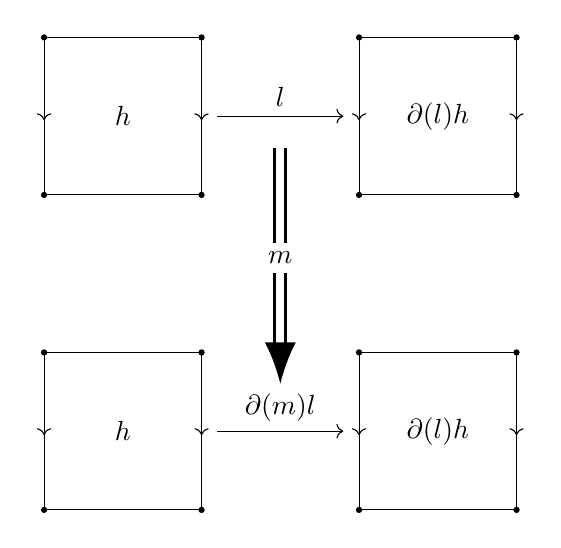
\begin{tikzpicture}[scale=2]
    \begin{scope}[xshift=0.0cm]
      \draw (0,0) to node[sloped] {\tikz{\draw[->](0,0)--(0.1,0);}} (0,-1);
      \draw (1,0) to node[sloped] {\tikz{\draw[->](0,0)--(0.1,0);}} (1,-1);
      \draw (0,0) to node[sloped] {\tikz{\draw[-](0,0)--(0.1,0);}} (1,0);
      \draw (0,-1) to node  {\tikz{\draw[-](0,0)--(0.1,0);}} (1,-1);
      \node at (1/2,-1/2) {$h$};
      \draw (0,0) to node {\tikz{\draw[-](0,0)--(0.1,0);}} (1,0);
      \draw (0,-1) to node {\tikz{\draw[-](0,0)--(0.1,0);}} (1,-1);
      \fill[black] (0,0) circle[radius=0.02];
      \fill[black] (1,0) circle[radius=0.02];
      \fill[black] (0,-1) circle[radius=0.02];
      \fill[black] (1,-1) circle[radius=0.02];
      \draw[->] (1.1,-1/2) to (1.9,-1/2);
      \node at (1.5,-1/2) [above]{$l$};
    \begin{scope}[xshift=2.0cm]
      \draw (0,0) to node[sloped] {\tikz{\draw[->](0,0)--(0.1,0);}} (0,-1);
      \draw (1,0) to node[sloped] {\tikz{\draw[->](0,0)--(0.1,0);}} (1,-1);
      \draw (0,0) to node[sloped] {\tikz{\draw[-](0,0)--(0.1,0);}} (1,0);
      \draw (0,-1) to node  {\tikz{\draw[-](0,0)--(0.1,0);}} (1,-1);
      \node at (1/2,-1/2) {$\del(l)h$};
      \draw (0,0) to node {\tikz{\draw[-](0,0)--(0.1,0);}} (1,0);
      \draw (0,-1) to node {\tikz{\draw[-](0,0)--(0.1,0);}} (1,-1);
      \fill[black] (0,0) circle[radius=0.02];
      \fill[black] (1,0) circle[radius=0.02];
      \fill[black] (0,-1) circle[radius=0.02];
      \fill[black] (1,-1) circle[radius=0.02];
	\end{scope}
	  \end{scope}
	  \begin{scope}[xshift=0.0cm, yshift=-2.0cm]
      \draw (0,0) to node[sloped] {\tikz{\draw[->](0,0)--(0.1,0);}} (0,-1);
      \draw (1,0) to node[sloped] {\tikz{\draw[->](0,0)--(0.1,0);}} (1,-1);
      \draw (0,0) to node[sloped] {\tikz{\draw[-](0,0)--(0.1,0);}} (1,0);
      \draw (0,-1) to node  {\tikz{\draw[-](0,0)--(0.1,0);}} (1,-1);
      \node at (1/2,-1/2) {$h$};
      \draw (0,0) to node {\tikz{\draw[-](0,0)--(0.1,0);}} (1,0);
      \draw (0,-1) to node {\tikz{\draw[-](0,0)--(0.1,0);}} (1,-1);
      \fill[black] (0,0) circle[radius=0.02];
      \fill[black] (1,0) circle[radius=0.02];
      \fill[black] (0,-1) circle[radius=0.02];
      \fill[black] (1,-1) circle[radius=0.02];
      \draw[->] (1.1,-1/2) to (1.9,-1/2);
      \node at (1.5,-1/2) [above]{$\del(m)l$};
    \begin{scope}[xshift=2.0cm]
      \draw (0,0) to node[sloped] {\tikz{\draw[->](0,0)--(0.1,0);}} (0,-1);
      \draw (1,0) to node[sloped] {\tikz{\draw[->](0,0)--(0.1,0);}} (1,-1);
      \draw (0,0) to node[sloped] {\tikz{\draw[-](0,0)--(0.1,0);}} (1,0);
      \draw (0,-1) to node  {\tikz{\draw[-](0,0)--(0.1,0);}} (1,-1);
      \node at (1/2,-1/2) {$\del(l)h$};
      \draw (0,0) to node {\tikz{\draw[-](0,0)--(0.1,0);}} (1,0);
      \draw (0,-1) to node {\tikz{\draw[-](0,0)--(0.1,0);}} (1,-1);
      \fill[black] (0,0) circle[radius=0.02];
      \fill[black] (1,0) circle[radius=0.02];
      \fill[black] (0,-1) circle[radius=0.02];
      \fill[black] (1,-1) circle[radius=0.02];
	\end{scope}
	  \end{scope}
	  \draw [line width=1pt, double distance=3pt, arrows = {-Latex[length=0pt 3 0]}] (1.5,-0.7) -- (1.5,-2.2);
      \node at (1.5, -1.4)  [fill=white]{$m$};
  \end{tikzpicture}
\end{center}
\caption{Diagram of $M$}
\label{d:fig_m}
\end{figure}

\begin{figure}
\begin{center}
  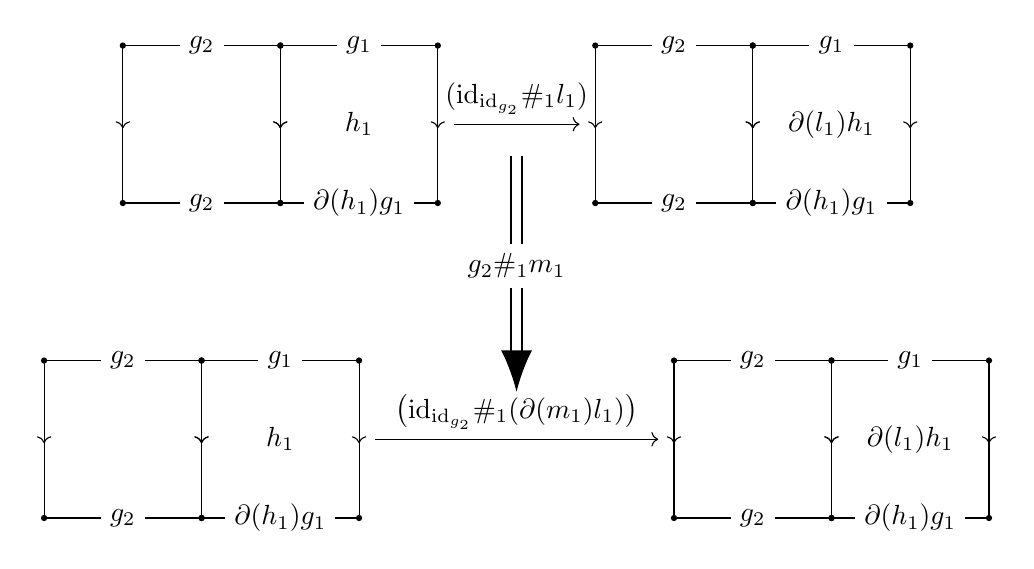
\begin{tikzpicture}[scale=2]
    \begin{scope}[xshift=0.0cm]
      \draw (0,0) to node[sloped] {\tikz{\draw[->](0,0)--(0.1,0);}} (0,-1);
      \draw (1,0) to node[sloped] {\tikz{\draw[->](0,0)--(0.1,0);}} (1,-1);
      \draw (0,0) to node[sloped] {\tikz{\draw[-](0,0)--(0.1,0);}} (1,0);
      \draw (0,-1) to node  {\tikz{\draw[-](0,0)--(0.1,0);}} (1,-1);
      \node at (1/2,-1/2) {$$};
      \draw (0,0) to node [fill=white]{$g_2$} (1,0);
      \draw (0,-1) to node [fill=white]{$g_2$} (1,-1);
      \fill[black] (0,0) circle[radius=0.02];
      \fill[black] (1,0) circle[radius=0.02];
      \fill[black] (0,-1) circle[radius=0.02];
      \fill[black] (1,-1) circle[radius=0.02];
      \draw[->] (2.1,-1/2) to (2.9,-1/2);
      \node at (2.5,-1/2) [above]{$({\rm id}_{{\rm id}_{g_2}} \#_1 l_1)$};
      \begin{scope}[xshift=1.0cm]
      \draw (0,0) to node[sloped] {\tikz{\draw[->](0,0)--(0.1,0);}} (0,-1);
      \draw (1,0) to node[sloped] {\tikz{\draw[->](0,0)--(0.1,0);}} (1,-1);
      \draw (0,0) to node[sloped] {\tikz{\draw[-](0,0)--(0.1,0);}} (1,0);
      \node at (1/2,-1/2) {$h_1$};
      \draw (0,0) to node [fill=white]{$g_1$} (1,0);
      \draw (0,-1) to node[fill=white]{$\del(h_1)g_1$} (1,-1);
      \fill[black] (0,0) circle[radius=0.02];
      \fill[black] (1,0) circle[radius=0.02];
      \fill[black] (0,-1) circle[radius=0.02];
      \fill[black] (1,-1) circle[radius=0.02];
	\end{scope}
    \begin{scope}[xshift=3.0cm]
      \draw (0,0) to node[sloped] {\tikz{\draw[->](0,0)--(0.1,0);}} (0,-1);
      \draw (1,0) to node[sloped] {\tikz{\draw[->](0,0)--(0.1,0);}} (1,-1);
      \draw (0,0) to node[sloped] {\tikz{\draw[-](0,0)--(0.1,0);}} (1,0);
      \draw (0,-1) to node  {\tikz{\draw[-](0,0)--(0.1,0);}} (1,-1);
      \node at (1/2,-1/2) {$$};
	 \draw (0,0) to node [fill=white]{$g_2$} (1,0);
      \draw (0,-1) to node [fill=white]{$g_2$} (1,-1);
      \fill[black] (0,0) circle[radius=0.02];
      \fill[black] (1,0) circle[radius=0.02];
      \fill[black] (0,-1) circle[radius=0.02];
      \fill[black] (1,-1) circle[radius=0.02];
	\end{scope}
	\begin{scope}[xshift=4.0cm]
      \draw (0,0) to node[sloped] {\tikz{\draw[->](0,0)--(0.1,0);}} (0,-1);
      \draw (1,0) to node[sloped] {\tikz{\draw[->](0,0)--(0.1,0);}} (1,-1);
      \draw (0,0) to node[sloped] {\tikz{\draw[-](0,0)--(0.1,0);}} (1,0);
      \draw (0,-1) to node  {\tikz{\draw[-](0,0)--(0.1,0);}} (1,-1);
      \node at (1/2,-1/2) {$\del(l_1)h_1$};
      \draw (0,0) to node [fill=white]{$g_1$} (1,0);
      \draw (0,-1) to node[fill=white]{$\del(h_1)g_1$} (1,-1);
      \fill[black] (0,0) circle[radius=0.02];
      \fill[black] (1,0) circle[radius=0.02];
      \fill[black] (0,-1) circle[radius=0.02];
      \fill[black] (1,-1) circle[radius=0.02];
	\end{scope}
	  \end{scope}
	 \begin{scope}[xshift=0cm, yshift=-2.0cm]
	 \draw[->] (1.6,-1/2) to (3.4,-1/2);
      \node at (2.5,-1/2) [above]{$\left({\rm id}_{{\rm id}_{g_2}} \#_1 (\del(m_1)l_1)\right)$};
	 \begin{scope}[xshift=-0.5cm]
      \draw (0,0) to node[sloped] {\tikz{\draw[->](0,0)--(0.1,0);}} (0,-1);
      \draw (1,0) to node[sloped] {\tikz{\draw[->](0,0)--(0.1,0);}} (1,-1);
      \draw (0,0) to node[sloped] {\tikz{\draw[-](0,0)--(0.1,0);}} (1,0);
      \draw (0,-1) to node  {\tikz{\draw[-](0,0)--(0.1,0);}} (1,-1);
      \node at (1/2,-1/2) {$$};
      \draw (0,0) to node [fill=white]{$g_2$} (1,0);
      \draw (0,-1) to node [fill=white]{$g_2$} (1,-1);
      \fill[black] (0,0) circle[radius=0.02];
      \fill[black] (1,0) circle[radius=0.02];
      \fill[black] (0,-1) circle[radius=0.02];
      \fill[black] (1,-1) circle[radius=0.02];
      \end{scope}
      \begin{scope}[xshift=0.5cm]
      \draw (0,0) to node[sloped] {\tikz{\draw[->](0,0)--(0.1,0);}} (0,-1);
      \draw (1,0) to node[sloped] {\tikz{\draw[->](0,0)--(0.1,0);}} (1,-1);
      \draw (0,0) to node[sloped] {\tikz{\draw[-](0,0)--(0.1,0);}} (1,0);
      \node at (1/2,-1/2) {$h_1$};
      \draw (0,0) to node [fill=white]{$g_1$} (1,0);
      \draw (0,-1) to node[fill=white]{$\del(h_1)g_1$} (1,-1);
      \fill[black] (0,0) circle[radius=0.02];
      \fill[black] (1,0) circle[radius=0.02];
      \fill[black] (0,-1) circle[radius=0.02];
      \fill[black] (1,-1) circle[radius=0.02];
	\end{scope}
    \begin{scope}[xshift=3.5cm]
      \draw (0,0) to node[sloped] {\tikz{\draw[->](0,0)--(0.1,0);}} (0,-1);
      \draw (1,0) to node[sloped] {\tikz{\draw[->](0,0)--(0.1,0);}} (1,-1);
      \draw (0,0) to node[sloped] {\tikz{\draw[-](0,0)--(0.1,0);}} (1,0);
      \draw (0,-1) to node  {\tikz{\draw[-](0,0)--(0.1,0);}} (1,-1);
      \node at (1/2,-1/2) {$$};
	 \draw (0,0) to node [fill=white]{$g_2$} (1,0);
      \draw (0,-1) to node [fill=white]{$g_2$} (1,-1);
      \fill[black] (0,0) circle[radius=0.02];
      \fill[black] (1,0) circle[radius=0.02];
      \fill[black] (0,-1) circle[radius=0.02];
      \fill[black] (1,-1) circle[radius=0.02];
	\end{scope}
	\begin{scope}[xshift=4.5cm]
      \draw (0,0) to node[sloped] {\tikz{\draw[->](0,0)--(0.1,0);}} (0,-1);
      \draw (1,0) to node[sloped] {\tikz{\draw[->](0,0)--(0.1,0);}} (1,-1);
      \draw (0,0) to node[sloped] {\tikz{\draw[-](0,0)--(0.1,0);}} (1,0);
      \draw (0,-1) to node  {\tikz{\draw[-](0,0)--(0.1,0);}} (1,-1);
      \node at (1/2,-1/2) {$\del(l_1)h_1$};
      \draw (0,0) to node [fill=white]{$g_1$} (1,0);
      \draw (0,-1) to node[fill=white]{$\del(h_1)g_1$} (1,-1);
      \fill[black] (0,0) circle[radius=0.02];
      \fill[black] (1,0) circle[radius=0.02];
      \fill[black] (0,-1) circle[radius=0.02];
      \fill[black] (1,-1) circle[radius=0.02];
	\end{scope}
	  \end{scope}
	  \draw [line width=1pt, double distance=3pt, arrows = {-Latex[length=0pt 3 0]}] (2.5,-0.7) -- (2.5,-2.2);
      \node at (2.5, -1.4)  [fill=white]{$g_2\#_1 m_1$};
  \end{tikzpicture}
\end{center}
\caption{Diagram of $g_2 \#_1 m_1$}
\label{d:g2_m1}
\end{figure}


For elements of $M$, there are four types of compositions: $\#_1, \#_2, \#_3$, and $\#_4$. Here, $\#_4$ denotes the vertical composition in $M$, while $\#_1, \#_2$ ,and  $\#_3$ denote horizontal compositions, defined in a similar manner as before.
For each $g_2, g_1 \in G$, $h_2, h_1\in H$, $l_2, l_1 \in L$, and $m_1, m_2 \in M$, we define
\[
g_2 \#_1 m_1  \coloneqq {\rm id}_{{\rm id}_{{\rm id}_{g_2}}} \#_1 m_1, \qquad m_2 \#_1 g_1  \coloneqq m_2 \#_1  {\rm id}_{{\rm id}_{{\rm id}_{g_1}}}.
\]
 These are represented in Figures~\ref{d:g2_m1} and~\ref{d:m2_g1}, respectively. 

\begin{figure}[!]
\begin{center}
  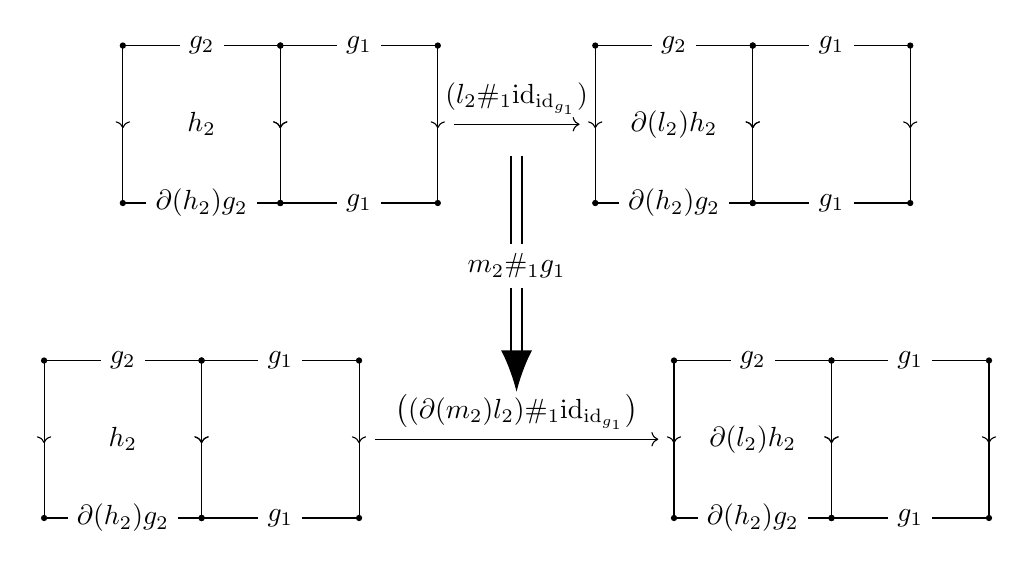
\begin{tikzpicture}[scale=2]
    \begin{scope}[xshift=0.0cm]
      \draw[->] (2.1,-1/2) to (2.9,-1/2);
      \node at (2.5,-1/2) [above]{$( l_2 \#_1  {\rm id}_{{\rm id}_{g_1}} )$};
      \draw (0,0) to node[sloped] {\tikz{\draw[->](0,0)--(0.1,0);}} (0,-1);
      \draw (1,0) to node[sloped] {\tikz{\draw[->](0,0)--(0.1,0);}} (1,-1);
      \draw (0,0) to node[sloped] {\tikz{\draw[-](0,0)--(0.1,0);}} (1,0);
      \draw (0,-1) to node  {\tikz{\draw[-](0,0)--(0.1,0);}} (1,-1);
      \node at (1/2,-1/2) {$h_2$};
      \draw (0,0) to node [fill=white]{$g_2$} (1,0);
      \draw (0,-1) to node [fill=white]{$\del(h_2)g_2$} (1,-1);
      \fill[black] (0,0) circle[radius=0.02];
      \fill[black] (1,0) circle[radius=0.02];
      \fill[black] (0,-1) circle[radius=0.02];
      \fill[black] (1,-1) circle[radius=0.02];
      \begin{scope}[xshift=1.0cm]
      \draw (0,0) to node[sloped] {\tikz{\draw[->](0,0)--(0.1,0);}} (0,-1);
      \draw (1,0) to node[sloped] {\tikz{\draw[->](0,0)--(0.1,0);}} (1,-1);
      \draw (0,0) to node[sloped] {\tikz{\draw[-](0,0)--(0.1,0);}} (1,0);
      \node at (1/2,-1/2) {$$};
      \draw (0,0) to node [fill=white]{$g_1$} (1,0);
      \draw (0,-1) to node[fill=white]{$g_1$} (1,-1);
      \fill[black] (0,0) circle[radius=0.02];
      \fill[black] (1,0) circle[radius=0.02];
      \fill[black] (0,-1) circle[radius=0.02];
      \fill[black] (1,-1) circle[radius=0.02];
	\end{scope}
    \begin{scope}[xshift=3.0cm]
      \draw (0,0) to node[sloped] {\tikz{\draw[->](0,0)--(0.1,0);}} (0,-1);
      \draw (1,0) to node[sloped] {\tikz{\draw[->](0,0)--(0.1,0);}} (1,-1);
      \draw (0,0) to node[sloped] {\tikz{\draw[-](0,0)--(0.1,0);}} (1,0);
      \draw (0,-1) to node  {\tikz{\draw[-](0,0)--(0.1,0);}} (1,-1);
      \node at (1/2,-1/2) {$\del(l_2)h_2$};
	 \draw (0,0) to node [fill=white]{$g_2$} (1,0);
      \draw (0,-1) to node [fill=white]{$\del(h_2)g_2$} (1,-1);
      \fill[black] (0,0) circle[radius=0.02];
      \fill[black] (1,0) circle[radius=0.02];
      \fill[black] (0,-1) circle[radius=0.02];
      \fill[black] (1,-1) circle[radius=0.02];
	\end{scope}
	\begin{scope}[xshift=4.0cm]
      \draw (0,0) to node[sloped] {\tikz{\draw[->](0,0)--(0.1,0);}} (0,-1);
      \draw (1,0) to node[sloped] {\tikz{\draw[->](0,0)--(0.1,0);}} (1,-1);
      \draw (0,0) to node[sloped] {\tikz{\draw[-](0,0)--(0.1,0);}} (1,0);
      \draw (0,-1) to node  {\tikz{\draw[-](0,0)--(0.1,0);}} (1,-1);
      \node at (1/2,-1/2) {$$};
      \draw (0,0) to node [fill=white]{$g_1$} (1,0);
      \draw (0,-1) to node[fill=white]{$g_1$} (1,-1);
      \fill[black] (0,0) circle[radius=0.02];
      \fill[black] (1,0) circle[radius=0.02];
      \fill[black] (0,-1) circle[radius=0.02];
      \fill[black] (1,-1) circle[radius=0.02];
	\end{scope}
	  \end{scope}
	 \begin{scope}[xshift=0cm, yshift=-2.0cm]
	 \draw[->] (1.6,-1/2) to (3.4,-1/2);
      \node at (2.5,-1/2) [above]{$\left( (\del(m_2)l_2) \#_1  {\rm id}_{{\rm id}_{g_1}}\right)$};
	 \begin{scope}[xshift=-0.5cm]
      \draw (0,0) to node[sloped] {\tikz{\draw[->](0,0)--(0.1,0);}} (0,-1);
      \draw (1,0) to node[sloped] {\tikz{\draw[->](0,0)--(0.1,0);}} (1,-1);
      \draw (0,0) to node[sloped] {\tikz{\draw[-](0,0)--(0.1,0);}} (1,0);
      \draw (0,-1) to node  {\tikz{\draw[-](0,0)--(0.1,0);}} (1,-1);
      \node at (1/2,-1/2) {$h_2$};
      \draw (0,0) to node [fill=white]{$g_2$} (1,0);
      \draw (0,-1) to node [fill=white]{$\del(h_2)g_2$} (1,-1);
      \fill[black] (0,0) circle[radius=0.02];
      \fill[black] (1,0) circle[radius=0.02];
      \fill[black] (0,-1) circle[radius=0.02];
      \fill[black] (1,-1) circle[radius=0.02];
      \end{scope}
      \begin{scope}[xshift=0.5cm]
      \draw (0,0) to node[sloped] {\tikz{\draw[->](0,0)--(0.1,0);}} (0,-1);
      \draw (1,0) to node[sloped] {\tikz{\draw[->](0,0)--(0.1,0);}} (1,-1);
      \draw (0,0) to node[sloped] {\tikz{\draw[-](0,0)--(0.1,0);}} (1,0);
      \node at (1/2,-1/2) {$$};
      \draw (0,0) to node [fill=white]{$g_1$} (1,0);
      \draw (0,-1) to node[fill=white]{$g_1$} (1,-1);
      \fill[black] (0,0) circle[radius=0.02];
      \fill[black] (1,0) circle[radius=0.02];
      \fill[black] (0,-1) circle[radius=0.02];
      \fill[black] (1,-1) circle[radius=0.02];
	\end{scope}
    \begin{scope}[xshift=3.5cm]
      \draw (0,0) to node[sloped] {\tikz{\draw[->](0,0)--(0.1,0);}} (0,-1);
      \draw (1,0) to node[sloped] {\tikz{\draw[->](0,0)--(0.1,0);}} (1,-1);
      \draw (0,0) to node[sloped] {\tikz{\draw[-](0,0)--(0.1,0);}} (1,0);
      \draw (0,-1) to node  {\tikz{\draw[-](0,0)--(0.1,0);}} (1,-1);
      \node at (1/2,-1/2) {$\del(l_2)h_2$};
      \draw (0,0) to node [fill=white]{$g_2$} (1,0);
      \draw (0,-1) to node [fill=white]{$\del(h_2)g_2$} (1,-1);
      \fill[black] (0,0) circle[radius=0.02];
      \fill[black] (1,0) circle[radius=0.02];
      \fill[black] (0,-1) circle[radius=0.02];
      \fill[black] (1,-1) circle[radius=0.02];
	\end{scope}
	\begin{scope}[xshift=4.5cm]
      \draw (0,0) to node[sloped] {\tikz{\draw[->](0,0)--(0.1,0);}} (0,-1);
      \draw (1,0) to node[sloped] {\tikz{\draw[->](0,0)--(0.1,0);}} (1,-1);
      \draw (0,0) to node[sloped] {\tikz{\draw[-](0,0)--(0.1,0);}} (1,0);
      \draw (0,-1) to node  {\tikz{\draw[-](0,0)--(0.1,0);}} (1,-1);
      \node at (1/2,-1/2) {$$};
      \draw (0,0) to node [fill=white]{$g_1$} (1,0);
      \draw (0,-1) to node[fill=white]{$g_1$} (1,-1);
      \fill[black] (0,0) circle[radius=0.02];
      \fill[black] (1,0) circle[radius=0.02];
      \fill[black] (0,-1) circle[radius=0.02];
      \fill[black] (1,-1) circle[radius=0.02];
	\end{scope}
	  \end{scope}
	  \draw [line width=1pt, double distance=3pt, arrows = {-Latex[length=0pt 3 0]}] (2.5,-0.7) -- (2.5,-2.2);
      \node at (2.5, -1.4)  [fill=white]{$m_2\#_1 g_1$};
  \end{tikzpicture}
\end{center}
\caption{Diagram of $m_2 \#_1 g_1$}
\label{d:m2_g1}
\end{figure}

For each $h_2, h_1\in H$, $l_2, l_1 \in L$, and $m_1, m_2 \in M$, we define 
\[
h_2 \#_2 m_1 \coloneqq {\rm id}_{{\rm id}_{h_2}} \#_2 m_1, \qquad m_2 \#_2 h_1 \coloneqq m_1 \#_2 {\rm id}_{{\rm id}_{h_1}},
\]
 which are represented in Figures~\ref{d:h2_m1} and~\ref{d:m2_h1}, respectively.

\begin{figure}
\begin{center}
  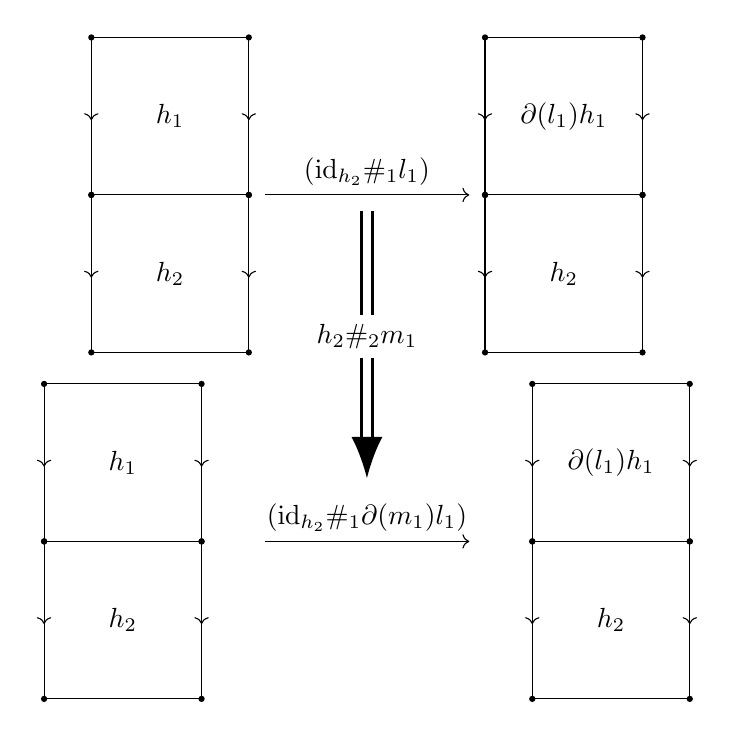
\begin{tikzpicture}[scale=2]
    \begin{scope}[xshift=0.0cm]
      \draw[->] (1.1,-1) to (2.4,-1);
      \node at (1.75,-1) [above]{$(   {\rm id}_{h_2}  \#_1 l_1 )$};
      \draw (0,0) to node[sloped] {\tikz{\draw[->](0,0)--(0.1,0);}} (0,-1);
      \draw (1,0) to node[sloped] {\tikz{\draw[->](0,0)--(0.1,0);}} (1,-1);
      \draw (0,0) to node[sloped] {\tikz{\draw[-](0,0)--(0.1,0);}} (1,0);
      \draw (0,-1) to node  {\tikz{\draw[-](0,0)--(0.1,0);}} (1,-1);
      \node at (1/2,-1/2) {$h_1$};
      \draw (0,0) to node {\tikz{\draw[-](0,0)--(0.1,0);}} (1,0);
      \draw (0,-1) to node {\tikz{\draw[-](0,0)--(0.1,0);}}(1,-1);
      \fill[black] (0,0) circle[radius=0.02];
      \fill[black] (1,0) circle[radius=0.02];
      \fill[black] (0,-1) circle[radius=0.02];
      \fill[black] (1,-1) circle[radius=0.02];
      \begin{scope}[yshift=-1.0cm]
      \draw (0,0) to node[sloped] {\tikz{\draw[->](0,0)--(0.1,0);}} (0,-1);
      \draw (1,0) to node[sloped] {\tikz{\draw[->](0,0)--(0.1,0);}} (1,-1);
      \draw (0,0) to node[sloped] {\tikz{\draw[-](0,0)--(0.1,0);}} (1,0);
      \node at (1/2,-1/2) {$h_2$};
      \draw (0,0) to node {\tikz{\draw[-](0,0)--(0.1,0);}} (1,0);
      \draw (0,-1) to node{\tikz{\draw[-](0,0)--(0.1,0);}} (1,-1);
      \fill[black] (0,0) circle[radius=0.02];
      \fill[black] (1,0) circle[radius=0.02];
      \fill[black] (0,-1) circle[radius=0.02];
      \fill[black] (1,-1) circle[radius=0.02];
	\end{scope}
    \begin{scope}[xshift=2.5cm]
      \draw (0,0) to node[sloped] {\tikz{\draw[->](0,0)--(0.1,0);}} (0,-1);
      \draw (1,0) to node[sloped] {\tikz{\draw[->](0,0)--(0.1,0);}} (1,-1);
      \draw (0,0) to node[sloped] {\tikz{\draw[-](0,0)--(0.1,0);}} (1,0);
      \draw (0,-1) to node  {\tikz{\draw[-](0,0)--(0.1,0);}} (1,-1);
      \node at (1/2,-1/2) {$\del(l_1)h_1$};
	 \draw (0,0) to node {\tikz{\draw[-](0,0)--(0.1,0);}} (1,0);
      \draw (0,-1) to node {\tikz{\draw[-](0,0)--(0.1,0);}} (1,-1);
      \fill[black] (0,0) circle[radius=0.02];
      \fill[black] (1,0) circle[radius=0.02];
      \fill[black] (0,-1) circle[radius=0.02];
      \fill[black] (1,-1) circle[radius=0.02];
	\end{scope}
	\begin{scope}[xshift=2.5cm, yshift=-1.0cm]
      \draw (0,0) to node[sloped] {\tikz{\draw[->](0,0)--(0.1,0);}} (0,-1);
      \draw (1,0) to node[sloped] {\tikz{\draw[->](0,0)--(0.1,0);}} (1,-1);
      \draw (0,0) to node[sloped] {\tikz{\draw[-](0,0)--(0.1,0);}} (1,0);
      \draw (0,-1) to node  {\tikz{\draw[-](0,0)--(0.1,0);}} (1,-1);
      \node at (1/2,-1/2) {$h_2$};
      \draw (0,0) to node {\tikz{\draw[-](0,0)--(0.1,0);}}(1,0);
      \draw (0,-1) to node{\tikz{\draw[-](0,0)--(0.1,0);}} (1,-1);
      \fill[black] (0,0) circle[radius=0.02];
      \fill[black] (1,0) circle[radius=0.02];
      \fill[black] (0,-1) circle[radius=0.02];
      \fill[black] (1,-1) circle[radius=0.02];
	\end{scope}
	  \end{scope}
	 \begin{scope}[xshift=0cm, yshift=-2.2cm]
	 \draw[->] (1.1,-1) to (2.4,-1);
      \node at (1.75,-1) [above]{$\left({\rm id}_{h_2}  \#_1\del(m_1) l_1\right)$};
	 \begin{scope}[xshift=-0.3cm]
      \draw (0,0) to node[sloped] {\tikz{\draw[->](0,0)--(0.1,0);}} (0,-1);
      \draw (1,0) to node[sloped] {\tikz{\draw[->](0,0)--(0.1,0);}} (1,-1);
      \draw (0,0) to node[sloped] {\tikz{\draw[-](0,0)--(0.1,0);}} (1,0);
      \draw (0,-1) to node  {\tikz{\draw[-](0,0)--(0.1,0);}} (1,-1);
      \node at (1/2,-1/2) {$h_1$};
      \draw (0,0) to node {\tikz{\draw[-](0,0)--(0.1,0);}} (1,0);
      \draw (0,-1) to node {\tikz{\draw[-](0,0)--(0.1,0);}} (1,-1);
      \fill[black] (0,0) circle[radius=0.02];
      \fill[black] (1,0) circle[radius=0.02];
      \fill[black] (0,-1) circle[radius=0.02];
      \fill[black] (1,-1) circle[radius=0.02];
      \end{scope}
      \begin{scope}[xshift=-0.3cm,yshift=-1.0cm]
      \draw (0,0) to node[sloped] {\tikz{\draw[->](0,0)--(0.1,0);}} (0,-1);
      \draw (1,0) to node[sloped] {\tikz{\draw[->](0,0)--(0.1,0);}} (1,-1);
      \draw (0,0) to node[sloped] {\tikz{\draw[-](0,0)--(0.1,0);}} (1,0);
      \node at (1/2,-1/2) {$ h_2$};
      \draw (0,0) to node {\tikz{\draw[-](0,0)--(0.1,0);}} (1,0);
      \draw (0,-1) to node{\tikz{\draw[-](0,0)--(0.1,0);}} (1,-1);
      \fill[black] (0,0) circle[radius=0.02];
      \fill[black] (1,0) circle[radius=0.02];
      \fill[black] (0,-1) circle[radius=0.02];
      \fill[black] (1,-1) circle[radius=0.02];
	\end{scope}
    \begin{scope}[xshift=2.8cm]
      \draw (0,0) to node[sloped] {\tikz{\draw[->](0,0)--(0.1,0);}} (0,-1);
      \draw (1,0) to node[sloped] {\tikz{\draw[->](0,0)--(0.1,0);}} (1,-1);
      \draw (0,0) to node[sloped] {\tikz{\draw[-](0,0)--(0.1,0);}} (1,0);
      \draw (0,-1) to node  {\tikz{\draw[-](0,0)--(0.1,0);}} (1,-1);
      \node at (1/2,-1/2) {$\del(l_1)h_1$};
      \draw (0,0) to node {\tikz{\draw[-](0,0)--(0.1,0);}} (1,0);
      \draw (0,-1) to node {\tikz{\draw[-](0,0)--(0.1,0);}} (1,-1);
      \fill[black] (0,0) circle[radius=0.02];
      \fill[black] (1,0) circle[radius=0.02];
      \fill[black] (0,-1) circle[radius=0.02];
      \fill[black] (1,-1) circle[radius=0.02];
	\end{scope}
	\begin{scope}[xshift=2.8cm,yshift=-1.0cm]
      \draw (0,0) to node[sloped] {\tikz{\draw[->](0,0)--(0.1,0);}} (0,-1);
      \draw (1,0) to node[sloped] {\tikz{\draw[->](0,0)--(0.1,0);}} (1,-1);
      \draw (0,0) to node[sloped] {\tikz{\draw[-](0,0)--(0.1,0);}} (1,0);
      \draw (0,-1) to node  {\tikz{\draw[-](0,0)--(0.1,0);}} (1,-1);
      \node at (1/2,-1/2) {$h_2$};
      \draw (0,0) to node {\tikz{\draw[-](0,0)--(0.1,0);}} (1,0);
      \draw (0,-1) to node{\tikz{\draw[-](0,0)--(0.1,0);}} (1,-1);
      \fill[black] (0,0) circle[radius=0.02];
      \fill[black] (1,0) circle[radius=0.02];
      \fill[black] (0,-1) circle[radius=0.02];
      \fill[black] (1,-1) circle[radius=0.02];
	\end{scope}
	  \end{scope}
	  \draw [line width=1pt, double distance=3pt, arrows = {-Latex[length=0pt 3 0]}] (1.75,-1.1) -- (1.75,-2.8);
      \node at (1.75, -1.9)  [fill=white]{$ h_2 \#_2 m_1$};
  \end{tikzpicture}
\end{center}
\caption{Diagram of $h_2 \#_2 m_1$}
\label{d:h2_m1}
\end{figure}

\begin{figure}
\begin{center}
  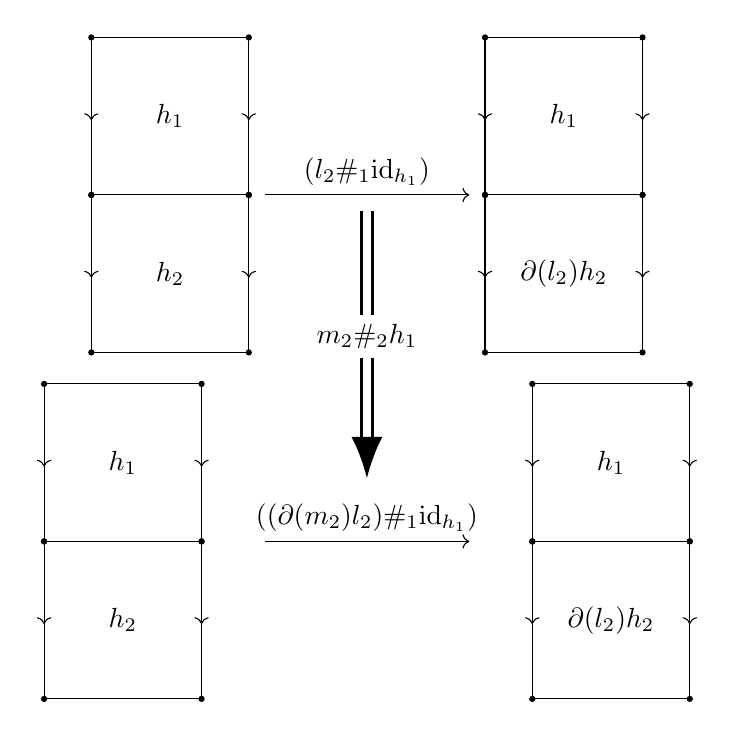
\begin{tikzpicture}[scale=2]
    \begin{scope}[xshift=0.0cm]
      \draw[->] (1.1,-1) to (2.4,-1);
      \node at (1.75,-1) [above]{$( l_2 \#_1  {\rm id}_{h_1} )$};
      \draw (0,0) to node[sloped] {\tikz{\draw[->](0,0)--(0.1,0);}} (0,-1);
      \draw (1,0) to node[sloped] {\tikz{\draw[->](0,0)--(0.1,0);}} (1,-1);
      \draw (0,0) to node[sloped] {\tikz{\draw[-](0,0)--(0.1,0);}} (1,0);
      \draw (0,-1) to node  {\tikz{\draw[-](0,0)--(0.1,0);}} (1,-1);
      \node at (1/2,-1/2) {$h_1$};
      \draw (0,0) to node {\tikz{\draw[-](0,0)--(0.1,0);}} (1,0);
      \draw (0,-1) to node {\tikz{\draw[-](0,0)--(0.1,0);}}(1,-1);
      \fill[black] (0,0) circle[radius=0.02];
      \fill[black] (1,0) circle[radius=0.02];
      \fill[black] (0,-1) circle[radius=0.02];
      \fill[black] (1,-1) circle[radius=0.02];
      \begin{scope}[yshift=-1.0cm]
      \draw (0,0) to node[sloped] {\tikz{\draw[->](0,0)--(0.1,0);}} (0,-1);
      \draw (1,0) to node[sloped] {\tikz{\draw[->](0,0)--(0.1,0);}} (1,-1);
      \draw (0,0) to node[sloped] {\tikz{\draw[-](0,0)--(0.1,0);}} (1,0);
      \node at (1/2,-1/2) {$h_2$};
      \draw (0,0) to node {\tikz{\draw[-](0,0)--(0.1,0);}} (1,0);
      \draw (0,-1) to node{\tikz{\draw[-](0,0)--(0.1,0);}} (1,-1);
      \fill[black] (0,0) circle[radius=0.02];
      \fill[black] (1,0) circle[radius=0.02];
      \fill[black] (0,-1) circle[radius=0.02];
      \fill[black] (1,-1) circle[radius=0.02];
	\end{scope}
    \begin{scope}[xshift=2.5cm]
      \draw (0,0) to node[sloped] {\tikz{\draw[->](0,0)--(0.1,0);}} (0,-1);
      \draw (1,0) to node[sloped] {\tikz{\draw[->](0,0)--(0.1,0);}} (1,-1);
      \draw (0,0) to node[sloped] {\tikz{\draw[-](0,0)--(0.1,0);}} (1,0);
      \draw (0,-1) to node  {\tikz{\draw[-](0,0)--(0.1,0);}} (1,-1);
      \node at (1/2,-1/2) {$h_1$};
	 \draw (0,0) to node {\tikz{\draw[-](0,0)--(0.1,0);}} (1,0);
      \draw (0,-1) to node {\tikz{\draw[-](0,0)--(0.1,0);}} (1,-1);
      \fill[black] (0,0) circle[radius=0.02];
      \fill[black] (1,0) circle[radius=0.02];
      \fill[black] (0,-1) circle[radius=0.02];
      \fill[black] (1,-1) circle[radius=0.02];
	\end{scope}
	\begin{scope}[xshift=2.5cm, yshift=-1.0cm]
      \draw (0,0) to node[sloped] {\tikz{\draw[->](0,0)--(0.1,0);}} (0,-1);
      \draw (1,0) to node[sloped] {\tikz{\draw[->](0,0)--(0.1,0);}} (1,-1);
      \draw (0,0) to node[sloped] {\tikz{\draw[-](0,0)--(0.1,0);}} (1,0);
      \draw (0,-1) to node  {\tikz{\draw[-](0,0)--(0.1,0);}} (1,-1);
      \node at (1/2,-1/2) {$\del(l_2)h_2$};
      \draw (0,0) to node {\tikz{\draw[-](0,0)--(0.1,0);}}(1,0);
      \draw (0,-1) to node{\tikz{\draw[-](0,0)--(0.1,0);}} (1,-1);
      \fill[black] (0,0) circle[radius=0.02];
      \fill[black] (1,0) circle[radius=0.02];
      \fill[black] (0,-1) circle[radius=0.02];
      \fill[black] (1,-1) circle[radius=0.02];
	\end{scope}
	  \end{scope}
	 \begin{scope}[xshift=0cm, yshift=-2.2cm]
	 \draw[->] (1.1,-1) to (2.4,-1);
      \node at (1.75,-1) [above]{$\left( (\del(m_2)l_2) \#_1  {\rm id}_{h_1}\right)$};
	 \begin{scope}[xshift=-0.3cm]
      \draw (0,0) to node[sloped] {\tikz{\draw[->](0,0)--(0.1,0);}} (0,-1);
      \draw (1,0) to node[sloped] {\tikz{\draw[->](0,0)--(0.1,0);}} (1,-1);
      \draw (0,0) to node[sloped] {\tikz{\draw[-](0,0)--(0.1,0);}} (1,0);
      \draw (0,-1) to node  {\tikz{\draw[-](0,0)--(0.1,0);}} (1,-1);
      \node at (1/2,-1/2) {$h_1$};
      \draw (0,0) to node {\tikz{\draw[-](0,0)--(0.1,0);}} (1,0);
      \draw (0,-1) to node {\tikz{\draw[-](0,0)--(0.1,0);}} (1,-1);
      \fill[black] (0,0) circle[radius=0.02];
      \fill[black] (1,0) circle[radius=0.02];
      \fill[black] (0,-1) circle[radius=0.02];
      \fill[black] (1,-1) circle[radius=0.02];
      \end{scope}
      \begin{scope}[xshift=-0.3cm,yshift=-1.0cm]
      \draw (0,0) to node[sloped] {\tikz{\draw[->](0,0)--(0.1,0);}} (0,-1);
      \draw (1,0) to node[sloped] {\tikz{\draw[->](0,0)--(0.1,0);}} (1,-1);
      \draw (0,0) to node[sloped] {\tikz{\draw[-](0,0)--(0.1,0);}} (1,0);
      \node at (1/2,-1/2) {$ h_2$};
      \draw (0,0) to node {\tikz{\draw[-](0,0)--(0.1,0);}} (1,0);
      \draw (0,-1) to node{\tikz{\draw[-](0,0)--(0.1,0);}} (1,-1);
      \fill[black] (0,0) circle[radius=0.02];
      \fill[black] (1,0) circle[radius=0.02];
      \fill[black] (0,-1) circle[radius=0.02];
      \fill[black] (1,-1) circle[radius=0.02];
	\end{scope}
    \begin{scope}[xshift=2.8cm]
      \draw (0,0) to node[sloped] {\tikz{\draw[->](0,0)--(0.1,0);}} (0,-1);
      \draw (1,0) to node[sloped] {\tikz{\draw[->](0,0)--(0.1,0);}} (1,-1);
      \draw (0,0) to node[sloped] {\tikz{\draw[-](0,0)--(0.1,0);}} (1,0);
      \draw (0,-1) to node  {\tikz{\draw[-](0,0)--(0.1,0);}} (1,-1);
      \node at (1/2,-1/2) {$h_1$};
      \draw (0,0) to node {\tikz{\draw[-](0,0)--(0.1,0);}} (1,0);
      \draw (0,-1) to node {\tikz{\draw[-](0,0)--(0.1,0);}} (1,-1);
      \fill[black] (0,0) circle[radius=0.02];
      \fill[black] (1,0) circle[radius=0.02];
      \fill[black] (0,-1) circle[radius=0.02];
      \fill[black] (1,-1) circle[radius=0.02];
	\end{scope}
	\begin{scope}[xshift=2.8cm,yshift=-1.0cm]
      \draw (0,0) to node[sloped] {\tikz{\draw[->](0,0)--(0.1,0);}} (0,-1);
      \draw (1,0) to node[sloped] {\tikz{\draw[->](0,0)--(0.1,0);}} (1,-1);
      \draw (0,0) to node[sloped] {\tikz{\draw[-](0,0)--(0.1,0);}} (1,0);
      \draw (0,-1) to node  {\tikz{\draw[-](0,0)--(0.1,0);}} (1,-1);
      \node at (1/2,-1/2) {$\del(l_2)h_2$};
      \draw (0,0) to node {\tikz{\draw[-](0,0)--(0.1,0);}} (1,0);
      \draw (0,-1) to node{\tikz{\draw[-](0,0)--(0.1,0);}} (1,-1);
      \fill[black] (0,0) circle[radius=0.02];
      \fill[black] (1,0) circle[radius=0.02];
      \fill[black] (0,-1) circle[radius=0.02];
      \fill[black] (1,-1) circle[radius=0.02];
	\end{scope}
	  \end{scope}
	  \draw [line width=1pt, double distance=3pt, arrows = {-Latex[length=0pt 3 0]}] (1.75,-1.1) -- (1.75,-2.8);
      \node at (1.75, -1.9)  [fill=white]{$m_2\#_2 h_1$};
  \end{tikzpicture}
\end{center}
\caption{Diagram of $m_2 \#_2 h_1$}
\label{d:m2_h1}
\end{figure}

For each $h\in H$, $l_2, l_1 \in L$, and $m_1, m_2 \in M$, we define
\[
l_2 \#_3 m_1 \coloneqq {\rm id}_{l_2} \#_3 m_1, \qquad m_2 \#_2 l_1 \coloneqq  m_2 \#_2 {\rm id}_{l_1},
\]
 which are represented in Figures~\ref{d:l2_m1} and~\ref{d:m2_l1}, respectively.

\begin{figure}
\begin{center}
  \begin{tikzpicture}[scale=2]
    \begin{scope}[xshift=0.0cm]
      \draw[->] (1.1,-1/2) to (2.4,-1/2);
      \node at (1.75,-1/2) [above]{$l_1$};
      \draw (0,0) to node[sloped] {\tikz{\draw[->](0,0)--(0.1,0);}} (0,-1);
      \draw (1,0) to node[sloped] {\tikz{\draw[->](0,0)--(0.1,0);}} (1,-1);
      \draw (0,0) to node[sloped] {\tikz{\draw[-](0,0)--(0.1,0);}} (1,0);
      \draw (0,-1) to node  {\tikz{\draw[-](0,0)--(0.1,0);}} (1,-1);
      \node at (1/2,-1/2) {$h$};
      \draw (0,0) to node {\tikz{\draw[-](0,0)--(0.1,0);}} (1,0);
      \draw (0,-1) to node {\tikz{\draw[-](0,0)--(0.1,0);}}(1,-1);
      \fill[black] (0,0) circle[radius=0.02];
      \fill[black] (1,0) circle[radius=0.02];
      \fill[black] (0,-1) circle[radius=0.02];
      \fill[black] (1,-1) circle[radius=0.02];   
	  \end{scope}
	  \begin{scope}[xshift=2.5cm]
      \draw[->] (1.1,-1/2) to (2.4,-1/2);
      \node at (1.75,-1/2) [above]{$l_2$};
      \draw (0,0) to node[sloped] {\tikz{\draw[->](0,0)--(0.1,0);}} (0,-1);
      \draw (1,0) to node[sloped] {\tikz{\draw[->](0,0)--(0.1,0);}} (1,-1);
      \draw (0,0) to node[sloped] {\tikz{\draw[-](0,0)--(0.1,0);}} (1,0);
      \draw (0,-1) to node  {\tikz{\draw[-](0,0)--(0.1,0);}} (1,-1);
      \node at (1/2,-1/2) {$\del(l_1)h$};
      \draw (0,0) to node {\tikz{\draw[-](0,0)--(0.1,0);}} (1,0);
      \draw (0,-1) to node {\tikz{\draw[-](0,0)--(0.1,0);}}(1,-1);
      \fill[black] (0,0) circle[radius=0.02];
      \fill[black] (1,0) circle[radius=0.02];
      \fill[black] (0,-1) circle[radius=0.02];
      \fill[black] (1,-1) circle[radius=0.02];   
	  \end{scope}
	    \begin{scope}[xshift=5.0cm]
      \draw (0,0) to node[sloped] {\tikz{\draw[->](0,0)--(0.1,0);}} (0,-1);
      \draw (1,0) to node[sloped] {\tikz{\draw[->](0,0)--(0.1,0);}} (1,-1);
      \draw (0,0) to node[sloped] {\tikz{\draw[-](0,0)--(0.1,0);}} (1,0);
      \draw (0,-1) to node  {\tikz{\draw[-](0,0)--(0.1,0);}} (1,-1);
      \node at (1/2,-1/2) {$\del(l_2 l_1)h$};
      \draw (0,0) to node {\tikz{\draw[-](0,0)--(0.1,0);}} (1,0);
      \draw (0,-1) to node {\tikz{\draw[-](0,0)--(0.1,0);}}(1,-1);
      \fill[black] (0,0) circle[radius=0.02];
      \fill[black] (1,0) circle[radius=0.02];
      \fill[black] (0,-1) circle[radius=0.02];
      \fill[black] (1,-1) circle[radius=0.02];   
	  \end{scope}
	 \begin{scope}[xshift=0cm, yshift=-2.2cm]
	 \begin{scope}[xshift=0.0cm]
      \draw[->] (1.1,-1/2) to (2.4,-1/2);
      \node at (1.75,-1/2) [above]{$\del(m_1)l_1$};
      \draw (0,0) to node[sloped] {\tikz{\draw[->](0,0)--(0.1,0);}} (0,-1);
      \draw (1,0) to node[sloped] {\tikz{\draw[->](0,0)--(0.1,0);}} (1,-1);
      \draw (0,0) to node[sloped] {\tikz{\draw[-](0,0)--(0.1,0);}} (1,0);
      \draw (0,-1) to node  {\tikz{\draw[-](0,0)--(0.1,0);}} (1,-1);
      \node at (1/2,-1/2) {$h_1$};
      \draw (0,0) to node {\tikz{\draw[-](0,0)--(0.1,0);}} (1,0);
      \draw (0,-1) to node {\tikz{\draw[-](0,0)--(0.1,0);}}(1,-1);
      \fill[black] (0,0) circle[radius=0.02];
      \fill[black] (1,0) circle[radius=0.02];
      \fill[black] (0,-1) circle[radius=0.02];
      \fill[black] (1,-1) circle[radius=0.02];   
	  \end{scope}
	  \begin{scope}[xshift=2.5cm]
      \draw[->] (1.1,-1/2) to (2.4,-1/2);
      \node at (1.75,-1/2) [above]{$l_2$};
      \draw (0,0) to node[sloped] {\tikz{\draw[->](0,0)--(0.1,0);}} (0,-1);
      \draw (1,0) to node[sloped] {\tikz{\draw[->](0,0)--(0.1,0);}} (1,-1);
      \draw (0,0) to node[sloped] {\tikz{\draw[-](0,0)--(0.1,0);}} (1,0);
      \draw (0,-1) to node  {\tikz{\draw[-](0,0)--(0.1,0);}} (1,-1);
      \node at (1/2,-1/2) {$\del(l_1)h_1$};
      \draw (0,0) to node {\tikz{\draw[-](0,0)--(0.1,0);}} (1,0);
      \draw (0,-1) to node {\tikz{\draw[-](0,0)--(0.1,0);}}(1,-1);
      \fill[black] (0,0) circle[radius=0.02];
      \fill[black] (1,0) circle[radius=0.02];
      \fill[black] (0,-1) circle[radius=0.02];
      \fill[black] (1,-1) circle[radius=0.02];   
	  \end{scope}
	    \begin{scope}[xshift=5.0cm]
      \draw (0,0) to node[sloped] {\tikz{\draw[->](0,0)--(0.1,0);}} (0,-1);
      \draw (1,0) to node[sloped] {\tikz{\draw[->](0,0)--(0.1,0);}} (1,-1);
      \draw (0,0) to node[sloped] {\tikz{\draw[-](0,0)--(0.1,0);}} (1,0);
      \draw (0,-1) to node  {\tikz{\draw[-](0,0)--(0.1,0);}} (1,-1);
      \node at (1/2,-1/2) {$\del(l_2 l_1)h_1$};
      \draw (0,0) to node {\tikz{\draw[-](0,0)--(0.1,0);}} (1,0);
      \draw (0,-1) to node {\tikz{\draw[-](0,0)--(0.1,0);}}(1,-1);
      \fill[black] (0,0) circle[radius=0.02];
      \fill[black] (1,0) circle[radius=0.02];
      \fill[black] (0,-1) circle[radius=0.02];
      \fill[black] (1,-1) circle[radius=0.02];   
	  \end{scope}
	  \end{scope}
	  \draw [line width=1pt, double distance=3pt, arrows = {-Latex[length=0pt 3 0]}] (3.0,-1.1) -- (3.0,-2.2);
      \node at (3.0, -1.5)  [fill=white]{${l_2} \#_3 m_1$};
  \end{tikzpicture}
\end{center}
\caption{Diagram of $l_2 \#_3 m_1$}
\label{d:l2_m1}
\end{figure}

\begin{figure}
\begin{center}
  \begin{tikzpicture}[scale=2]
    \begin{scope}[xshift=0.0cm]
      \draw[->] (1.1,-1/2) to (2.4,-1/2);
      \node at (1.75,-1/2) [above]{$l_1$};
      \draw (0,0) to node[sloped] {\tikz{\draw[->](0,0)--(0.1,0);}} (0,-1);
      \draw (1,0) to node[sloped] {\tikz{\draw[->](0,0)--(0.1,0);}} (1,-1);
      \draw (0,0) to node[sloped] {\tikz{\draw[-](0,0)--(0.1,0);}} (1,0);
      \draw (0,-1) to node  {\tikz{\draw[-](0,0)--(0.1,0);}} (1,-1);
      \node at (1/2,-1/2) {$h$};
      \draw (0,0) to node {\tikz{\draw[-](0,0)--(0.1,0);}} (1,0);
      \draw (0,-1) to node {\tikz{\draw[-](0,0)--(0.1,0);}}(1,-1);
      \fill[black] (0,0) circle[radius=0.02];
      \fill[black] (1,0) circle[radius=0.02];
      \fill[black] (0,-1) circle[radius=0.02];
      \fill[black] (1,-1) circle[radius=0.02];   
	  \end{scope}
	  \begin{scope}[xshift=2.5cm]
      \draw[->] (1.1,-1/2) to (2.4,-1/2);
      \node at (1.75,-1/2) [above]{$l_2$};
      \draw (0,0) to node[sloped] {\tikz{\draw[->](0,0)--(0.1,0);}} (0,-1);
      \draw (1,0) to node[sloped] {\tikz{\draw[->](0,0)--(0.1,0);}} (1,-1);
      \draw (0,0) to node[sloped] {\tikz{\draw[-](0,0)--(0.1,0);}} (1,0);
      \draw (0,-1) to node  {\tikz{\draw[-](0,0)--(0.1,0);}} (1,-1);
      \node at (1/2,-1/2) {$\del(l_1)h$};
      \draw (0,0) to node {\tikz{\draw[-](0,0)--(0.1,0);}} (1,0);
      \draw (0,-1) to node {\tikz{\draw[-](0,0)--(0.1,0);}}(1,-1);
      \fill[black] (0,0) circle[radius=0.02];
      \fill[black] (1,0) circle[radius=0.02];
      \fill[black] (0,-1) circle[radius=0.02];
      \fill[black] (1,-1) circle[radius=0.02];   
	  \end{scope}
	    \begin{scope}[xshift=5.0cm]
      \draw (0,0) to node[sloped] {\tikz{\draw[->](0,0)--(0.1,0);}} (0,-1);
      \draw (1,0) to node[sloped] {\tikz{\draw[->](0,0)--(0.1,0);}} (1,-1);
      \draw (0,0) to node[sloped] {\tikz{\draw[-](0,0)--(0.1,0);}} (1,0);
      \draw (0,-1) to node  {\tikz{\draw[-](0,0)--(0.1,0);}} (1,-1);
      \node at (1/2,-1/2) {$\del(l_2 l_1)h$};
      \draw (0,0) to node {\tikz{\draw[-](0,0)--(0.1,0);}} (1,0);
      \draw (0,-1) to node {\tikz{\draw[-](0,0)--(0.1,0);}}(1,-1);
      \fill[black] (0,0) circle[radius=0.02];
      \fill[black] (1,0) circle[radius=0.02];
      \fill[black] (0,-1) circle[radius=0.02];
      \fill[black] (1,-1) circle[radius=0.02];   
	  \end{scope}
	 \begin{scope}[xshift=0cm, yshift=-2.2cm]
	 \begin{scope}[xshift=0.0cm]
      \draw[->] (1.1,-1/2) to (2.4,-1/2);
      \node at (1.75,-1/2) [above]{$l_1$};
      \draw (0,0) to node[sloped] {\tikz{\draw[->](0,0)--(0.1,0);}} (0,-1);
      \draw (1,0) to node[sloped] {\tikz{\draw[->](0,0)--(0.1,0);}} (1,-1);
      \draw (0,0) to node[sloped] {\tikz{\draw[-](0,0)--(0.1,0);}} (1,0);
      \draw (0,-1) to node  {\tikz{\draw[-](0,0)--(0.1,0);}} (1,-1);
      \node at (1/2,-1/2) {$h_1$};
      \draw (0,0) to node {\tikz{\draw[-](0,0)--(0.1,0);}} (1,0);
      \draw (0,-1) to node {\tikz{\draw[-](0,0)--(0.1,0);}}(1,-1);
      \fill[black] (0,0) circle[radius=0.02];
      \fill[black] (1,0) circle[radius=0.02];
      \fill[black] (0,-1) circle[radius=0.02];
      \fill[black] (1,-1) circle[radius=0.02];   
	  \end{scope}
	  \begin{scope}[xshift=2.5cm]
      \draw[->] (1.1,-1/2) to (2.4,-1/2);
      \node at (1.75,-1/2) [above]{$\del(m_2)l_2$};
      \draw (0,0) to node[sloped] {\tikz{\draw[->](0,0)--(0.1,0);}} (0,-1);
      \draw (1,0) to node[sloped] {\tikz{\draw[->](0,0)--(0.1,0);}} (1,-1);
      \draw (0,0) to node[sloped] {\tikz{\draw[-](0,0)--(0.1,0);}} (1,0);
      \draw (0,-1) to node  {\tikz{\draw[-](0,0)--(0.1,0);}} (1,-1);
      \node at (1/2,-1/2) {$\del(l_1)h_1$};
      \draw (0,0) to node {\tikz{\draw[-](0,0)--(0.1,0);}} (1,0);
      \draw (0,-1) to node {\tikz{\draw[-](0,0)--(0.1,0);}}(1,-1);
      \fill[black] (0,0) circle[radius=0.02];
      \fill[black] (1,0) circle[radius=0.02];
      \fill[black] (0,-1) circle[radius=0.02];
      \fill[black] (1,-1) circle[radius=0.02];   
	  \end{scope}
	    \begin{scope}[xshift=5.0cm]
      \draw (0,0) to node[sloped] {\tikz{\draw[->](0,0)--(0.1,0);}} (0,-1);
      \draw (1,0) to node[sloped] {\tikz{\draw[->](0,0)--(0.1,0);}} (1,-1);
      \draw (0,0) to node[sloped] {\tikz{\draw[-](0,0)--(0.1,0);}} (1,0);
      \draw (0,-1) to node  {\tikz{\draw[-](0,0)--(0.1,0);}} (1,-1);
      \node at (1/2,-1/2) {$\del(l_2 l_1)h_1$};
      \draw (0,0) to node {\tikz{\draw[-](0,0)--(0.1,0);}} (1,0);
      \draw (0,-1) to node {\tikz{\draw[-](0,0)--(0.1,0);}}(1,-1);
      \fill[black] (0,0) circle[radius=0.02];
      \fill[black] (1,0) circle[radius=0.02];
      \fill[black] (0,-1) circle[radius=0.02];
      \fill[black] (1,-1) circle[radius=0.02];   
	  \end{scope}
	  \end{scope}
	  \draw [line width=1pt, double distance=3pt, arrows = {-Latex[length=0pt 3 0]}] (3.0,-1.1) -- (3.0,-2.2);
      \node at (3.0, -1.5)  [fill=white]{$ m_2 \#_3 {l_1} $};
  \end{tikzpicture}
\end{center}
\caption{Diagram of $m_2 \#_3 l_1$}
\label{d:m2_l1}
\end{figure}

The LL-Peiffer lifting is a one-dimensional higher analogue of the ordinary Peiffer lifting. For each $l_1,l_2 \in L$, we have the following relation:
\begin{align*}
\del \{l_2 , l_1 \}_{LL} \act{\del l_2}l_1 l_2 = l_2 l_1. \\
\end{align*}
Using 
\[
\act{\del l_2}l_1 l_2 = \left({\rm id}_{\del l_2} \#_2 l_1\right) \#_3 \left(l_2 \#_2 {\rm id}_{e_H}\right), \qquad l_2 l_1 = \left(l_2 \#_2 {\rm id}_{\del l_1}\right) \#_3 \left({\rm id}_{e_H} \#_2 l_1\right),
\]
we can describe $\{l_2 , l_1 \}_{LL}$ as shown in Figure~\ref{d:LL_lift}.

\begin{figure}
\begin{center}
  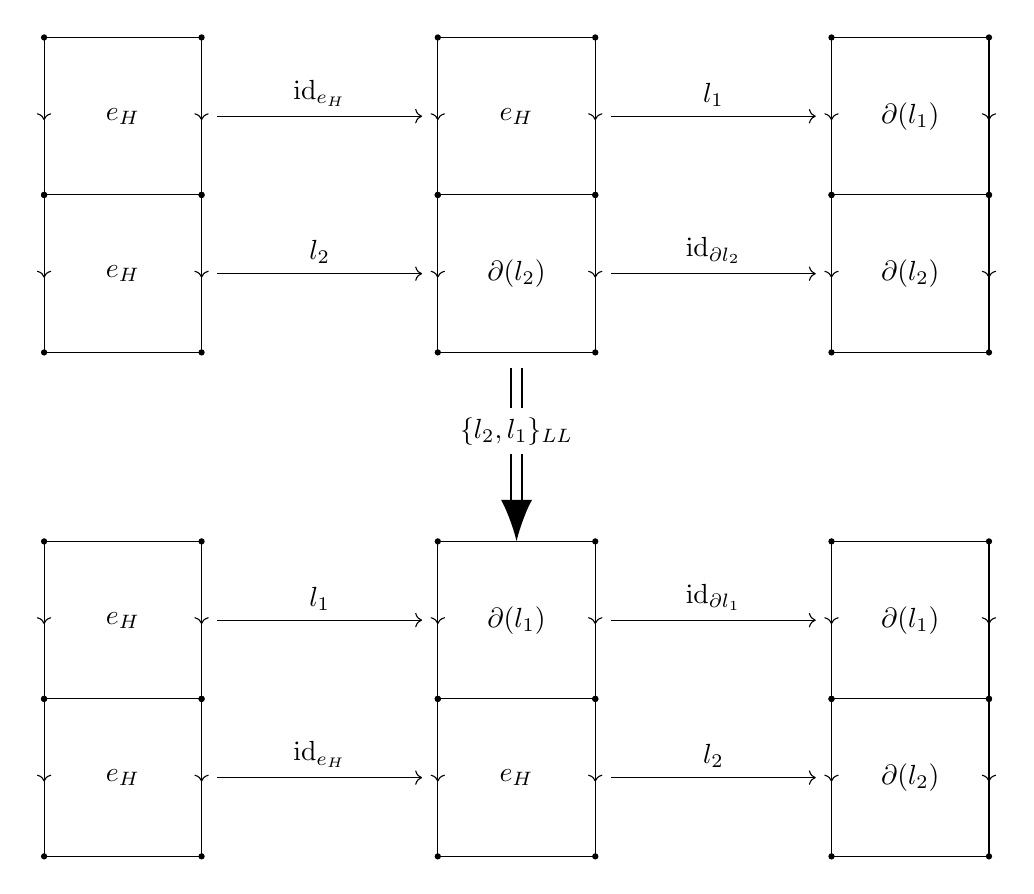
\begin{tikzpicture}[scale=2]
    \begin{scope}[xshift=0.0cm]
      \draw[->] (1.1,-1/2) to (2.4,-1/2);
      \node at (1.75,-1/2) [above]{${\rm id}_{e_H}$};
      \draw (0,0) to node[sloped] {\tikz{\draw[->](0,0)--(0.1,0);}} (0,-1);
      \draw (1,0) to node[sloped] {\tikz{\draw[->](0,0)--(0.1,0);}} (1,-1);
      \draw (0,0) to node[sloped] {\tikz{\draw[-](0,0)--(0.1,0);}} (1,0);
      \draw (0,-1) to node  {\tikz{\draw[-](0,0)--(0.1,0);}} (1,-1);
      \node at (1/2,-1/2) {$e_H$};
      \draw (0,0) to node {\tikz{\draw[-](0,0)--(0.1,0);}} (1,0);
      \draw (0,-1) to node {\tikz{\draw[-](0,0)--(0.1,0);}}(1,-1);
      \fill[black] (0,0) circle[radius=0.02];
      \fill[black] (1,0) circle[radius=0.02];
      \fill[black] (0,-1) circle[radius=0.02];
      \fill[black] (1,-1) circle[radius=0.02];   
	  \end{scope}
	  \begin{scope}[xshift=2.5cm]
      \draw[->] (1.1,-1/2) to (2.4,-1/2);
      \node at (1.75,-1/2) [above]{$l_1$};
      \draw (0,0) to node[sloped] {\tikz{\draw[->](0,0)--(0.1,0);}} (0,-1);
      \draw (1,0) to node[sloped] {\tikz{\draw[->](0,0)--(0.1,0);}} (1,-1);
      \draw (0,0) to node[sloped] {\tikz{\draw[-](0,0)--(0.1,0);}} (1,0);
      \draw (0,-1) to node  {\tikz{\draw[-](0,0)--(0.1,0);}} (1,-1);
      \node at (1/2,-1/2) {$e_H$};
      \draw (0,0) to node {\tikz{\draw[-](0,0)--(0.1,0);}} (1,0);
      \draw (0,-1) to node {\tikz{\draw[-](0,0)--(0.1,0);}}(1,-1);
      \fill[black] (0,0) circle[radius=0.02];
      \fill[black] (1,0) circle[radius=0.02];
      \fill[black] (0,-1) circle[radius=0.02];
      \fill[black] (1,-1) circle[radius=0.02];   
	  \end{scope}
	    \begin{scope}[xshift=5.0cm]
      \draw (0,0) to node[sloped] {\tikz{\draw[->](0,0)--(0.1,0);}} (0,-1);
      \draw (1,0) to node[sloped] {\tikz{\draw[->](0,0)--(0.1,0);}} (1,-1);
      \draw (0,0) to node[sloped] {\tikz{\draw[-](0,0)--(0.1,0);}} (1,0);
      \draw (0,-1) to node  {\tikz{\draw[-](0,0)--(0.1,0);}} (1,-1);
      \node at (1/2,-1/2) {$\del(l_1)$};
      \draw (0,0) to node {\tikz{\draw[-](0,0)--(0.1,0);}} (1,0);
      \draw (0,-1) to node {\tikz{\draw[-](0,0)--(0.1,0);}}(1,-1);
      \fill[black] (0,0) circle[radius=0.02];
      \fill[black] (1,0) circle[radius=0.02];
      \fill[black] (0,-1) circle[radius=0.02];
      \fill[black] (1,-1) circle[radius=0.02];   
	  \end{scope}
	   \begin{scope}[yshift=-1.0cm]
	   \begin{scope}[xshift=0.0cm]
      \draw[->] (1.1,-1/2) to (2.4,-1/2);
      \node at (1.75,-1/2) [above]{$l_2$};
      \draw (0,0) to node[sloped] {\tikz{\draw[->](0,0)--(0.1,0);}} (0,-1);
      \draw (1,0) to node[sloped] {\tikz{\draw[->](0,0)--(0.1,0);}} (1,-1);
      \draw (0,0) to node[sloped] {\tikz{\draw[-](0,0)--(0.1,0);}} (1,0);
      \draw (0,-1) to node  {\tikz{\draw[-](0,0)--(0.1,0);}} (1,-1);
      \node at (1/2,-1/2) {$e_H$};
      \draw (0,0) to node {\tikz{\draw[-](0,0)--(0.1,0);}} (1,0);
      \draw (0,-1) to node {\tikz{\draw[-](0,0)--(0.1,0);}}(1,-1);
      \fill[black] (0,0) circle[radius=0.02];
      \fill[black] (1,0) circle[radius=0.02];
      \fill[black] (0,-1) circle[radius=0.02];
      \fill[black] (1,-1) circle[radius=0.02];   
	  \end{scope}
	  \begin{scope}[xshift=2.5cm]
      \draw[->] (1.1,-1/2) to (2.4,-1/2);
      \node at (1.75,-1/2) [above]{${\rm id}_{\del l_2}$};
      \draw (0,0) to node[sloped] {\tikz{\draw[->](0,0)--(0.1,0);}} (0,-1);
      \draw (1,0) to node[sloped] {\tikz{\draw[->](0,0)--(0.1,0);}} (1,-1);
      \draw (0,0) to node[sloped] {\tikz{\draw[-](0,0)--(0.1,0);}} (1,0);
      \draw (0,-1) to node  {\tikz{\draw[-](0,0)--(0.1,0);}} (1,-1);
      \node at (1/2,-1/2) {$\del(l_2)$};
      \draw (0,0) to node {\tikz{\draw[-](0,0)--(0.1,0);}} (1,0);
      \draw (0,-1) to node {\tikz{\draw[-](0,0)--(0.1,0);}}(1,-1);
      \fill[black] (0,0) circle[radius=0.02];
      \fill[black] (1,0) circle[radius=0.02];
      \fill[black] (0,-1) circle[radius=0.02];
      \fill[black] (1,-1) circle[radius=0.02];   
	  \end{scope}
	    \begin{scope}[xshift=5.0cm]
      \draw (0,0) to node[sloped] {\tikz{\draw[->](0,0)--(0.1,0);}} (0,-1);
      \draw (1,0) to node[sloped] {\tikz{\draw[->](0,0)--(0.1,0);}} (1,-1);
      \draw (0,0) to node[sloped] {\tikz{\draw[-](0,0)--(0.1,0);}} (1,0);
      \draw (0,-1) to node  {\tikz{\draw[-](0,0)--(0.1,0);}} (1,-1);
      \node at (1/2,-1/2) {$\del(l_2)$};
      \draw (0,0) to node {\tikz{\draw[-](0,0)--(0.1,0);}} (1,0);
      \draw (0,-1) to node {\tikz{\draw[-](0,0)--(0.1,0);}}(1,-1);
      \fill[black] (0,0) circle[radius=0.02];
      \fill[black] (1,0) circle[radius=0.02];
      \fill[black] (0,-1) circle[radius=0.02];
      \fill[black] (1,-1) circle[radius=0.02];   
	  \end{scope}
	  \end{scope}
	  
	 \begin{scope}[xshift=0cm, yshift=-3.2cm]
	  \begin{scope}[xshift=0.0cm]
      \draw[->] (1.1,-1/2) to (2.4,-1/2);
      \node at (1.75,-1/2) [above]{$l_1$};
      \draw (0,0) to node[sloped] {\tikz{\draw[->](0,0)--(0.1,0);}} (0,-1);
      \draw (1,0) to node[sloped] {\tikz{\draw[->](0,0)--(0.1,0);}} (1,-1);
      \draw (0,0) to node[sloped] {\tikz{\draw[-](0,0)--(0.1,0);}} (1,0);
      \draw (0,-1) to node  {\tikz{\draw[-](0,0)--(0.1,0);}} (1,-1);
      \node at (1/2,-1/2) {${e_H}$};
      \draw (0,0) to node {\tikz{\draw[-](0,0)--(0.1,0);}} (1,0);
      \draw (0,-1) to node {\tikz{\draw[-](0,0)--(0.1,0);}}(1,-1);
      \fill[black] (0,0) circle[radius=0.02];
      \fill[black] (1,0) circle[radius=0.02];
      \fill[black] (0,-1) circle[radius=0.02];
      \fill[black] (1,-1) circle[radius=0.02];   
	  \end{scope}
	  \begin{scope}[xshift=2.5cm]
      \draw[->] (1.1,-1/2) to (2.4,-1/2);
      \node at (1.75,-1/2) [above]{${\rm id}_{\del l_1}$};
      \draw (0,0) to node[sloped] {\tikz{\draw[->](0,0)--(0.1,0);}} (0,-1);
      \draw (1,0) to node[sloped] {\tikz{\draw[->](0,0)--(0.1,0);}} (1,-1);
      \draw (0,0) to node[sloped] {\tikz{\draw[-](0,0)--(0.1,0);}} (1,0);
      \draw (0,-1) to node  {\tikz{\draw[-](0,0)--(0.1,0);}} (1,-1);
      \node at (1/2,-1/2) {$\del(l_1)$};
      \draw (0,0) to node {\tikz{\draw[-](0,0)--(0.1,0);}} (1,0);
      \draw (0,-1) to node {\tikz{\draw[-](0,0)--(0.1,0);}}(1,-1);
      \fill[black] (0,0) circle[radius=0.02];
      \fill[black] (1,0) circle[radius=0.02];
      \fill[black] (0,-1) circle[radius=0.02];
      \fill[black] (1,-1) circle[radius=0.02];   
	  \end{scope}
	    \begin{scope}[xshift=5.0cm]
      \draw (0,0) to node[sloped] {\tikz{\draw[->](0,0)--(0.1,0);}} (0,-1);
      \draw (1,0) to node[sloped] {\tikz{\draw[->](0,0)--(0.1,0);}} (1,-1);
      \draw (0,0) to node[sloped] {\tikz{\draw[-](0,0)--(0.1,0);}} (1,0);
      \draw (0,-1) to node  {\tikz{\draw[-](0,0)--(0.1,0);}} (1,-1);
      \node at (1/2,-1/2) {$\del(l_1)$};
      \draw (0,0) to node {\tikz{\draw[-](0,0)--(0.1,0);}} (1,0);
      \draw (0,-1) to node {\tikz{\draw[-](0,0)--(0.1,0);}}(1,-1);
      \fill[black] (0,0) circle[radius=0.02];
      \fill[black] (1,0) circle[radius=0.02];
      \fill[black] (0,-1) circle[radius=0.02];
      \fill[black] (1,-1) circle[radius=0.02];   
	  \end{scope}
	   \begin{scope}[yshift=-1.0cm]
	   \begin{scope}[xshift=0.0cm]
      \draw[->] (1.1,-1/2) to (2.4,-1/2);
      \node at (1.75,-1/2) [above]{${\rm id}_{e_H}$};
      \draw (0,0) to node[sloped] {\tikz{\draw[->](0,0)--(0.1,0);}} (0,-1);
      \draw (1,0) to node[sloped] {\tikz{\draw[->](0,0)--(0.1,0);}} (1,-1);
      \draw (0,0) to node[sloped] {\tikz{\draw[-](0,0)--(0.1,0);}} (1,0);
      \draw (0,-1) to node  {\tikz{\draw[-](0,0)--(0.1,0);}} (1,-1);
      \node at (1/2,-1/2) {$e_H$};
      \draw (0,0) to node {\tikz{\draw[-](0,0)--(0.1,0);}} (1,0);
      \draw (0,-1) to node {\tikz{\draw[-](0,0)--(0.1,0);}}(1,-1);
      \fill[black] (0,0) circle[radius=0.02];
      \fill[black] (1,0) circle[radius=0.02];
      \fill[black] (0,-1) circle[radius=0.02];
      \fill[black] (1,-1) circle[radius=0.02];   
	  \end{scope}
	  \begin{scope}[xshift=2.5cm]
      \draw[->] (1.1,-1/2) to (2.4,-1/2);
      \node at (1.75,-1/2) [above]{$l_2$};
      \draw (0,0) to node[sloped] {\tikz{\draw[->](0,0)--(0.1,0);}} (0,-1);
      \draw (1,0) to node[sloped] {\tikz{\draw[->](0,0)--(0.1,0);}} (1,-1);
      \draw (0,0) to node[sloped] {\tikz{\draw[-](0,0)--(0.1,0);}} (1,0);
      \draw (0,-1) to node  {\tikz{\draw[-](0,0)--(0.1,0);}} (1,-1);
      \node at (1/2,-1/2) {$e_H$};
      \draw (0,0) to node {\tikz{\draw[-](0,0)--(0.1,0);}} (1,0);
      \draw (0,-1) to node {\tikz{\draw[-](0,0)--(0.1,0);}}(1,-1);
      \fill[black] (0,0) circle[radius=0.02];
      \fill[black] (1,0) circle[radius=0.02];
      \fill[black] (0,-1) circle[radius=0.02];
      \fill[black] (1,-1) circle[radius=0.02];   
	  \end{scope}
	    \begin{scope}[xshift=5.0cm]
      \draw (0,0) to node[sloped] {\tikz{\draw[->](0,0)--(0.1,0);}} (0,-1);
      \draw (1,0) to node[sloped] {\tikz{\draw[->](0,0)--(0.1,0);}} (1,-1);
      \draw (0,0) to node[sloped] {\tikz{\draw[-](0,0)--(0.1,0);}} (1,0);
      \draw (0,-1) to node  {\tikz{\draw[-](0,0)--(0.1,0);}} (1,-1);
      \node at (1/2,-1/2) {$\del(l_2)$};
      \draw (0,0) to node {\tikz{\draw[-](0,0)--(0.1,0);}} (1,0);
      \draw (0,-1) to node {\tikz{\draw[-](0,0)--(0.1,0);}}(1,-1);
      \fill[black] (0,0) circle[radius=0.02];
      \fill[black] (1,0) circle[radius=0.02];
      \fill[black] (0,-1) circle[radius=0.02];
      \fill[black] (1,-1) circle[radius=0.02];   
	  \end{scope}
	  \end{scope}
	  \end{scope}
	  \draw [line width=1pt, double distance=3pt, arrows = {-Latex[length=0pt 3 0]}] (3.0,-2.1) -- (3.0,-3.2);
      \node at (3.0, -2.5)  [fill=white]{$ \{l_2, l_1\}_{LL} $};
  \end{tikzpicture}
\end{center}
\caption{Diagram of LL-Peiffer lifting}
\label{d:LL_lift}
\end{figure}

The meanings of Properties~\ref{lhmnr}, \ref{rhmnr}, \ref{lrhmnr} and~\ref{yanBt} of a 3-crossed module can be understood diagrammatically.  In particular, Property~\ref{lhmnr} can be represented as in Figure~\ref{d:rel_of_lhmn}.

\begin{figure}
\begin{center}
\scalebox{0.8}{
  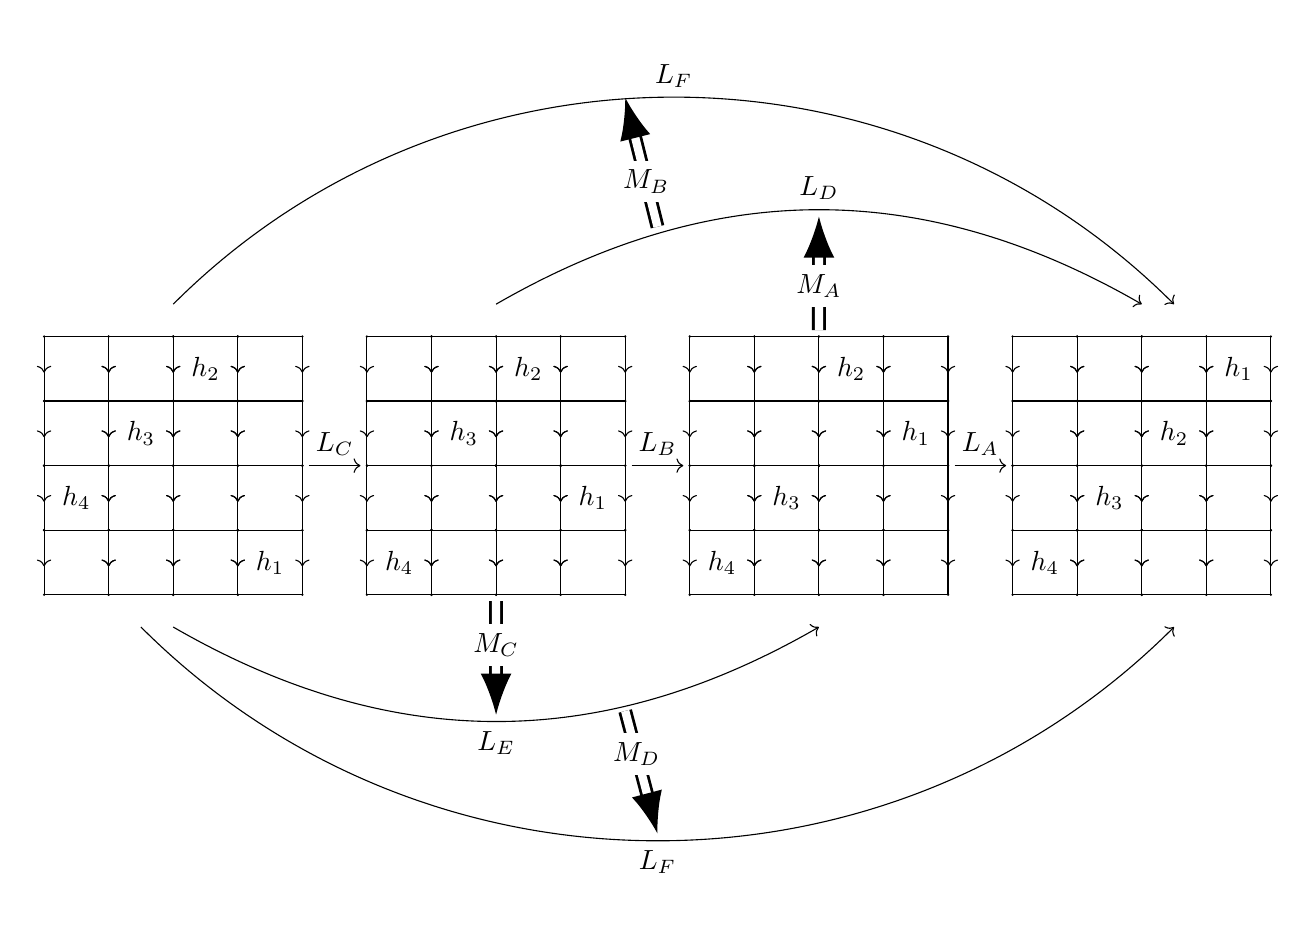
\begin{tikzpicture}[scale=0.82]
  \begin{scope}[xshift=0.0cm]
  \draw[->] (4.1,-2) to (4.9,-2);
      \node at (4.5,-2) [above]{$L_C$};
  	\begin{scope}[xshift=0.0cm]
	      \draw (0,0) to node[sloped] {\tikz{\draw[->](0,0)--(0.1,0);}} (0,-1);
	      \draw (1,0) to node[sloped] {\tikz{\draw[->](0,0)--(0.1,0);}} (1,-1);
	      \draw (0,0) to node[sloped] {\tikz{\draw[-](0,0)--(0.1,0);}} (1,0);
	      \draw (0,-1) to node  {\tikz{\draw[-](0,0)--(0.1,0);}} (1,-1);
	      \node at (1/2,-1/2) {$$};
	      \draw (0,0) to node {\tikz{\draw[-](0,0)--(0.1,0);}}(1,0);
	      \draw (0,-1) to node {\tikz{\draw[-](0,0)--(0.1,0);}} (1,-1);
	      \fill[black] (0,0) circle[radius=0.02];
	      \fill[black] (1,0) circle[radius=0.02];
	      \fill[black] (0,-1) circle[radius=0.02];
	      \fill[black] (1,-1) circle[radius=0.02];
	    \begin{scope}[xshift=1.0cm]
	      \draw (0,0) to node[sloped] {\tikz{\draw[->](0,0)--(0.1,0);}} (0,-1);
	      \draw (1,0) to node[sloped] {\tikz{\draw[->](0,0)--(0.1,0);}} (1,-1);
	      \draw (0,0) to node[sloped] {\tikz{\draw[-](0,0)--(0.1,0);}} (1,0);
	      \draw (0,-1) to node  {\tikz{\draw[-](0,0)--(0.1,0);}} (1,-1);
	      \node at (1/2,-1/2) {$$};
	      \draw (0,0) to node {\tikz{\draw[-](0,0)--(0.1,0);}} (1,0);
	      \draw (0,-1) to node {\tikz{\draw[-](0,0)--(0.1,0);}} (1,-1);
	      \fill[black] (0,0) circle[radius=0.02];
	      \fill[black] (1,0) circle[radius=0.02];
	      \fill[black] (0,-1) circle[radius=0.02];
	      \fill[black] (1,-1) circle[radius=0.02];
	    \end{scope}
	    	 \begin{scope}[xshift=2.0cm]
	      \draw (0,0) to node[sloped] {\tikz{\draw[->](0,0)--(0.1,0);}} (0,-1);
	      \draw (1,0) to node[sloped] {\tikz{\draw[->](0,0)--(0.1,0);}} (1,-1);
	      \draw (0,0) to node[sloped] {\tikz{\draw[-](0,0)--(0.1,0);}} (1,0);
	      \draw (0,-1) to node  {\tikz{\draw[-](0,0)--(0.1,0);}} (1,-1);
	      \node at (1/2,-1/2) {$h_2$};
	      \draw (0,0) to node {\tikz{\draw[-](0,0)--(0.1,0);}} (1,0);
	      \draw (0,-1) to node {\tikz{\draw[-](0,0)--(0.1,0);}} (1,-1);
	      \fill[black] (0,0) circle[radius=0.02];
	      \fill[black] (1,0) circle[radius=0.02];
	      \fill[black] (0,-1) circle[radius=0.02];
	      \fill[black] (1,-1) circle[radius=0.02];
	    \end{scope}
	     \begin{scope}[xshift=3.0cm]
	      \draw (0,0) to node[sloped] {\tikz{\draw[->](0,0)--(0.1,0);}} (0,-1);
	      \draw (1,0) to node[sloped] {\tikz{\draw[->](0,0)--(0.1,0);}} (1,-1);
	      \draw (0,0) to node[sloped] {\tikz{\draw[-](0,0)--(0.1,0);}} (1,0);
	      \draw (0,-1) to node  {\tikz{\draw[-](0,0)--(0.1,0);}} (1,-1);
	      \node at (1/2,-1/2) {$$};
	      \draw (0,0) to node {\tikz{\draw[-](0,0)--(0.1,0);}} (1,0);
	      \draw (0,-1) to node {\tikz{\draw[-](0,0)--(0.1,0);}} (1,-1);
	      \fill[black] (0,0) circle[radius=0.02];
	      \fill[black] (1,0) circle[radius=0.02];
	      \fill[black] (0,-1) circle[radius=0.02];
	      \fill[black] (1,-1) circle[radius=0.02];
	    \end{scope}
	     \end{scope}
	     %%%%%%%%%%%%%%%%%%%%%
	\begin{scope}[yshift=-1.0cm]
  	\begin{scope}[xshift=0.0cm]
	      \draw (0,0) to node[sloped] {\tikz{\draw[->](0,0)--(0.1,0);}} (0,-1);
	      \draw (1,0) to node[sloped] {\tikz{\draw[->](0,0)--(0.1,0);}} (1,-1);
	      \draw (0,0) to node[sloped] {\tikz{\draw[-](0,0)--(0.1,0);}} (1,0);
	      \draw (0,-1) to node  {\tikz{\draw[-](0,0)--(0.1,0);}} (1,-1);
	      \node at (1/2,-1/2) {$$};
	      \draw (0,0) to node {\tikz{\draw[-](0,0)--(0.1,0);}}(1,0);
	      \draw (0,-1) to node {\tikz{\draw[-](0,0)--(0.1,0);}} (1,-1);
	      \fill[black] (0,0) circle[radius=0.02];
	      \fill[black] (1,0) circle[radius=0.02];
	      \fill[black] (0,-1) circle[radius=0.02];
	      \fill[black] (1,-1) circle[radius=0.02];
	      \end{scope}
	    \begin{scope}[xshift=1.0cm]
	      \draw (0,0) to node[sloped] {\tikz{\draw[->](0,0)--(0.1,0);}} (0,-1);
	      \draw (1,0) to node[sloped] {\tikz{\draw[->](0,0)--(0.1,0);}} (1,-1);
	      \draw (0,0) to node[sloped] {\tikz{\draw[-](0,0)--(0.1,0);}} (1,0);
	      \draw (0,-1) to node  {\tikz{\draw[-](0,0)--(0.1,0);}} (1,-1);
	      \node at (1/2,-1/2) {$h_3$};
	      \draw (0,0) to node {\tikz{\draw[-](0,0)--(0.1,0);}} (1,0);
	      \draw (0,-1) to node {\tikz{\draw[-](0,0)--(0.1,0);}} (1,-1);
	      \fill[black] (0,0) circle[radius=0.02];
	      \fill[black] (1,0) circle[radius=0.02];
	      \fill[black] (0,-1) circle[radius=0.02];
	      \fill[black] (1,-1) circle[radius=0.02];
	    \end{scope}
	    	 \begin{scope}[xshift=2.0cm]
	      \draw (0,0) to node[sloped] {\tikz{\draw[->](0,0)--(0.1,0);}} (0,-1);
	      \draw (1,0) to node[sloped] {\tikz{\draw[->](0,0)--(0.1,0);}} (1,-1);
	      \draw (0,0) to node[sloped] {\tikz{\draw[-](0,0)--(0.1,0);}} (1,0);
	      \draw (0,-1) to node  {\tikz{\draw[-](0,0)--(0.1,0);}} (1,-1);
	      \node at (1/2,-1/2) {$$};
	      \draw (0,0) to node {\tikz{\draw[-](0,0)--(0.1,0);}} (1,0);
	      \draw (0,-1) to node {\tikz{\draw[-](0,0)--(0.1,0);}} (1,-1);
	      \fill[black] (0,0) circle[radius=0.02];
	      \fill[black] (1,0) circle[radius=0.02];
	      \fill[black] (0,-1) circle[radius=0.02];
	      \fill[black] (1,-1) circle[radius=0.02];
	    \end{scope}
	     \begin{scope}[xshift=3.0cm]
	      \draw (0,0) to node[sloped] {\tikz{\draw[->](0,0)--(0.1,0);}} (0,-1);
	      \draw (1,0) to node[sloped] {\tikz{\draw[->](0,0)--(0.1,0);}} (1,-1);
	      \draw (0,0) to node[sloped] {\tikz{\draw[-](0,0)--(0.1,0);}} (1,0);
	      \draw (0,-1) to node  {\tikz{\draw[-](0,0)--(0.1,0);}} (1,-1);
	      \node at (1/2,-1/2) {$$};
	      \draw (0,0) to node {\tikz{\draw[-](0,0)--(0.1,0);}} (1,0);
	      \draw (0,-1) to node {\tikz{\draw[-](0,0)--(0.1,0);}} (1,-1);
	      \fill[black] (0,0) circle[radius=0.02];
	      \fill[black] (1,0) circle[radius=0.02];
	      \fill[black] (0,-1) circle[radius=0.02];
	      \fill[black] (1,-1) circle[radius=0.02];
	    \end{scope}
	     \end{scope}
	       %%%%%%%%%%%%%%%%%%%%%
	     \begin{scope}[yshift=-2.0cm]
  	\begin{scope}[xshift=0.0cm]
	      \draw (0,0) to node[sloped] {\tikz{\draw[->](0,0)--(0.1,0);}} (0,-1);
	      \draw (1,0) to node[sloped] {\tikz{\draw[->](0,0)--(0.1,0);}} (1,-1);
	      \draw (0,0) to node[sloped] {\tikz{\draw[-](0,0)--(0.1,0);}} (1,0);
	      \draw (0,-1) to node  {\tikz{\draw[-](0,0)--(0.1,0);}} (1,-1);
	      \node at (1/2,-1/2) {$h_4$};
	      \draw (0,0) to node {\tikz{\draw[-](0,0)--(0.1,0);}}(1,0);
	      \draw (0,-1) to node {\tikz{\draw[-](0,0)--(0.1,0);}} (1,-1);
	      \fill[black] (0,0) circle[radius=0.02];
	      \fill[black] (1,0) circle[radius=0.02];
	      \fill[black] (0,-1) circle[radius=0.02];
	      \fill[black] (1,-1) circle[radius=0.02];
	      \end{scope}
	    \begin{scope}[xshift=1.0cm]
	      \draw (0,0) to node[sloped] {\tikz{\draw[->](0,0)--(0.1,0);}} (0,-1);
	      \draw (1,0) to node[sloped] {\tikz{\draw[->](0,0)--(0.1,0);}} (1,-1);
	      \draw (0,0) to node[sloped] {\tikz{\draw[-](0,0)--(0.1,0);}} (1,0);
	      \draw (0,-1) to node  {\tikz{\draw[-](0,0)--(0.1,0);}} (1,-1);
	      \node at (1/2,-1/2) {$$};
	      \draw (0,0) to node {\tikz{\draw[-](0,0)--(0.1,0);}} (1,0);
	      \draw (0,-1) to node {\tikz{\draw[-](0,0)--(0.1,0);}} (1,-1);
	      \fill[black] (0,0) circle[radius=0.02];
	      \fill[black] (1,0) circle[radius=0.02];
	      \fill[black] (0,-1) circle[radius=0.02];
	      \fill[black] (1,-1) circle[radius=0.02];
	    \end{scope}
	    	 \begin{scope}[xshift=2.0cm]
	      \draw (0,0) to node[sloped] {\tikz{\draw[->](0,0)--(0.1,0);}} (0,-1);
	      \draw (1,0) to node[sloped] {\tikz{\draw[->](0,0)--(0.1,0);}} (1,-1);
	      \draw (0,0) to node[sloped] {\tikz{\draw[-](0,0)--(0.1,0);}} (1,0);
	      \draw (0,-1) to node  {\tikz{\draw[-](0,0)--(0.1,0);}} (1,-1);
	      \node at (1/2,-1/2) {$$};
	      \draw (0,0) to node {\tikz{\draw[-](0,0)--(0.1,0);}} (1,0);
	      \draw (0,-1) to node {\tikz{\draw[-](0,0)--(0.1,0);}} (1,-1);
	      \fill[black] (0,0) circle[radius=0.02];
	      \fill[black] (1,0) circle[radius=0.02];
	      \fill[black] (0,-1) circle[radius=0.02];
	      \fill[black] (1,-1) circle[radius=0.02];
	    \end{scope}
	     \begin{scope}[xshift=3.0cm]
	      \draw (0,0) to node[sloped] {\tikz{\draw[->](0,0)--(0.1,0);}} (0,-1);
	      \draw (1,0) to node[sloped] {\tikz{\draw[->](0,0)--(0.1,0);}} (1,-1);
	      \draw (0,0) to node[sloped] {\tikz{\draw[-](0,0)--(0.1,0);}} (1,0);
	      \draw (0,-1) to node  {\tikz{\draw[-](0,0)--(0.1,0);}} (1,-1);
	      \node at (1/2,-1/2) {$$};
	      \draw (0,0) to node {\tikz{\draw[-](0,0)--(0.1,0);}} (1,0);
	      \draw (0,-1) to node {\tikz{\draw[-](0,0)--(0.1,0);}} (1,-1);
	      \fill[black] (0,0) circle[radius=0.02];
	      \fill[black] (1,0) circle[radius=0.02];
	      \fill[black] (0,-1) circle[radius=0.02];
	      \fill[black] (1,-1) circle[radius=0.02];
	    \end{scope}
	     \end{scope}
	       %%%%%%%%%%%%%%%%%%%%%
    \begin{scope}[yshift=-3.0cm]
  	\begin{scope}[xshift=0.0cm]
	      \draw (0,0) to node[sloped] {\tikz{\draw[->](0,0)--(0.1,0);}} (0,-1);
	      \draw (1,0) to node[sloped] {\tikz{\draw[->](0,0)--(0.1,0);}} (1,-1);
	      \draw (0,0) to node[sloped] {\tikz{\draw[-](0,0)--(0.1,0);}} (1,0);
	      \draw (0,-1) to node  {\tikz{\draw[-](0,0)--(0.1,0);}} (1,-1);
	      \node at (1/2,-1/2) {$$};
	      \draw (0,0) to node {\tikz{\draw[-](0,0)--(0.1,0);}}(1,0);
	      \draw (0,-1) to node {\tikz{\draw[-](0,0)--(0.1,0);}} (1,-1);
	      \fill[black] (0,0) circle[radius=0.02];
	      \fill[black] (1,0) circle[radius=0.02];
	      \fill[black] (0,-1) circle[radius=0.02];
	      \fill[black] (1,-1) circle[radius=0.02];
	      \end{scope}
	    \begin{scope}[xshift=1.0cm]
	      \draw (0,0) to node[sloped] {\tikz{\draw[->](0,0)--(0.1,0);}} (0,-1);
	      \draw (1,0) to node[sloped] {\tikz{\draw[->](0,0)--(0.1,0);}} (1,-1);
	      \draw (0,0) to node[sloped] {\tikz{\draw[-](0,0)--(0.1,0);}} (1,0);
	      \draw (0,-1) to node  {\tikz{\draw[-](0,0)--(0.1,0);}} (1,-1);
	      \node at (1/2,-1/2) {$$};
	      \draw (0,0) to node {\tikz{\draw[-](0,0)--(0.1,0);}} (1,0);
	      \draw (0,-1) to node {\tikz{\draw[-](0,0)--(0.1,0);}} (1,-1);
	      \fill[black] (0,0) circle[radius=0.02];
	      \fill[black] (1,0) circle[radius=0.02];
	      \fill[black] (0,-1) circle[radius=0.02];
	      \fill[black] (1,-1) circle[radius=0.02];
	    \end{scope}
	    	 \begin{scope}[xshift=2.0cm]
	      \draw (0,0) to node[sloped] {\tikz{\draw[->](0,0)--(0.1,0);}} (0,-1);
	      \draw (1,0) to node[sloped] {\tikz{\draw[->](0,0)--(0.1,0);}} (1,-1);
	      \draw (0,0) to node[sloped] {\tikz{\draw[-](0,0)--(0.1,0);}} (1,0);
	      \draw (0,-1) to node  {\tikz{\draw[-](0,0)--(0.1,0);}} (1,-1);
	      \node at (1/2,-1/2) {$$};
	      \draw (0,0) to node {\tikz{\draw[-](0,0)--(0.1,0);}} (1,0);
	      \draw (0,-1) to node {\tikz{\draw[-](0,0)--(0.1,0);}} (1,-1);
	      \fill[black] (0,0) circle[radius=0.02];
	      \fill[black] (1,0) circle[radius=0.02];
	      \fill[black] (0,-1) circle[radius=0.02];
	      \fill[black] (1,-1) circle[radius=0.02];
	    \end{scope}
	     \begin{scope}[xshift=3.0cm]
	      \draw (0,0) to node[sloped] {\tikz{\draw[->](0,0)--(0.1,0);}} (0,-1);
	      \draw (1,0) to node[sloped] {\tikz{\draw[->](0,0)--(0.1,0);}} (1,-1);
	      \draw (0,0) to node[sloped] {\tikz{\draw[-](0,0)--(0.1,0);}} (1,0);
	      \draw (0,-1) to node  {\tikz{\draw[-](0,0)--(0.1,0);}} (1,-1);
	      \node at (1/2,-1/2) {$h_1$};
	      \draw (0,0) to node {\tikz{\draw[-](0,0)--(0.1,0);}} (1,0);
	      \draw (0,-1) to node {\tikz{\draw[-](0,0)--(0.1,0);}} (1,-1);
	      \fill[black] (0,0) circle[radius=0.02];
	      \fill[black] (1,0) circle[radius=0.02];
	      \fill[black] (0,-1) circle[radius=0.02];
	      \fill[black] (1,-1) circle[radius=0.02];
	    \end{scope}
	     \end{scope}
	      \end{scope}
	     %%%%%%%%%%%%%%%%
	     %%%%%%%%%%%%%%%%
	     %%%%%%%%%%%%%%%
	     %%%%%%%%%%%%%%%%
	       \begin{scope}[xshift=5.0cm]
  \draw[->] (4.1,-2) to (4.9,-2);
      \node at (4.5,-2) [above]{$L_B$};
  	\begin{scope}[xshift=0.0cm]
	      \draw (0,0) to node[sloped] {\tikz{\draw[->](0,0)--(0.1,0);}} (0,-1);
	      \draw (1,0) to node[sloped] {\tikz{\draw[->](0,0)--(0.1,0);}} (1,-1);
	      \draw (0,0) to node[sloped] {\tikz{\draw[-](0,0)--(0.1,0);}} (1,0);
	      \draw (0,-1) to node  {\tikz{\draw[-](0,0)--(0.1,0);}} (1,-1);
	      \node at (1/2,-1/2) {$$};
	      \draw (0,0) to node {\tikz{\draw[-](0,0)--(0.1,0);}}(1,0);
	      \draw (0,-1) to node {\tikz{\draw[-](0,0)--(0.1,0);}} (1,-1);
	      \fill[black] (0,0) circle[radius=0.02];
	      \fill[black] (1,0) circle[radius=0.02];
	      \fill[black] (0,-1) circle[radius=0.02];
	      \fill[black] (1,-1) circle[radius=0.02];
	    \begin{scope}[xshift=1.0cm]
	      \draw (0,0) to node[sloped] {\tikz{\draw[->](0,0)--(0.1,0);}} (0,-1);
	      \draw (1,0) to node[sloped] {\tikz{\draw[->](0,0)--(0.1,0);}} (1,-1);
	      \draw (0,0) to node[sloped] {\tikz{\draw[-](0,0)--(0.1,0);}} (1,0);
	      \draw (0,-1) to node  {\tikz{\draw[-](0,0)--(0.1,0);}} (1,-1);
	      \node at (1/2,-1/2) {$$};
	      \draw (0,0) to node {\tikz{\draw[-](0,0)--(0.1,0);}} (1,0);
	      \draw (0,-1) to node {\tikz{\draw[-](0,0)--(0.1,0);}} (1,-1);
	      \fill[black] (0,0) circle[radius=0.02];
	      \fill[black] (1,0) circle[radius=0.02];
	      \fill[black] (0,-1) circle[radius=0.02];
	      \fill[black] (1,-1) circle[radius=0.02];
	    \end{scope}
	    	 \begin{scope}[xshift=2.0cm]
	      \draw (0,0) to node[sloped] {\tikz{\draw[->](0,0)--(0.1,0);}} (0,-1);
	      \draw (1,0) to node[sloped] {\tikz{\draw[->](0,0)--(0.1,0);}} (1,-1);
	      \draw (0,0) to node[sloped] {\tikz{\draw[-](0,0)--(0.1,0);}} (1,0);
	      \draw (0,-1) to node  {\tikz{\draw[-](0,0)--(0.1,0);}} (1,-1);
	      \node at (1/2,-1/2) {$h_2$};
	      \draw (0,0) to node {\tikz{\draw[-](0,0)--(0.1,0);}} (1,0);
	      \draw (0,-1) to node {\tikz{\draw[-](0,0)--(0.1,0);}} (1,-1);
	      \fill[black] (0,0) circle[radius=0.02];
	      \fill[black] (1,0) circle[radius=0.02];
	      \fill[black] (0,-1) circle[radius=0.02];
	      \fill[black] (1,-1) circle[radius=0.02];
	    \end{scope}
	     \begin{scope}[xshift=3.0cm]
	      \draw (0,0) to node[sloped] {\tikz{\draw[->](0,0)--(0.1,0);}} (0,-1);
	      \draw (1,0) to node[sloped] {\tikz{\draw[->](0,0)--(0.1,0);}} (1,-1);
	      \draw (0,0) to node[sloped] {\tikz{\draw[-](0,0)--(0.1,0);}} (1,0);
	      \draw (0,-1) to node  {\tikz{\draw[-](0,0)--(0.1,0);}} (1,-1);
	      \node at (1/2,-1/2) {$$};
	      \draw (0,0) to node {\tikz{\draw[-](0,0)--(0.1,0);}} (1,0);
	      \draw (0,-1) to node {\tikz{\draw[-](0,0)--(0.1,0);}} (1,-1);
	      \fill[black] (0,0) circle[radius=0.02];
	      \fill[black] (1,0) circle[radius=0.02];
	      \fill[black] (0,-1) circle[radius=0.02];
	      \fill[black] (1,-1) circle[radius=0.02];
	    \end{scope}
	     \end{scope}
	     %%%%%%%%%%%%%%%%%%%%%
	\begin{scope}[yshift=-1.0cm]
  	\begin{scope}[xshift=0.0cm]
	      \draw (0,0) to node[sloped] {\tikz{\draw[->](0,0)--(0.1,0);}} (0,-1);
	      \draw (1,0) to node[sloped] {\tikz{\draw[->](0,0)--(0.1,0);}} (1,-1);
	      \draw (0,0) to node[sloped] {\tikz{\draw[-](0,0)--(0.1,0);}} (1,0);
	      \draw (0,-1) to node  {\tikz{\draw[-](0,0)--(0.1,0);}} (1,-1);
	      \node at (1/2,-1/2) {$$};
	      \draw (0,0) to node {\tikz{\draw[-](0,0)--(0.1,0);}}(1,0);
	      \draw (0,-1) to node {\tikz{\draw[-](0,0)--(0.1,0);}} (1,-1);
	      \fill[black] (0,0) circle[radius=0.02];
	      \fill[black] (1,0) circle[radius=0.02];
	      \fill[black] (0,-1) circle[radius=0.02];
	      \fill[black] (1,-1) circle[radius=0.02];
	      \end{scope}
	    \begin{scope}[xshift=1.0cm]
	      \draw (0,0) to node[sloped] {\tikz{\draw[->](0,0)--(0.1,0);}} (0,-1);
	      \draw (1,0) to node[sloped] {\tikz{\draw[->](0,0)--(0.1,0);}} (1,-1);
	      \draw (0,0) to node[sloped] {\tikz{\draw[-](0,0)--(0.1,0);}} (1,0);
	      \draw (0,-1) to node  {\tikz{\draw[-](0,0)--(0.1,0);}} (1,-1);
	      \node at (1/2,-1/2) {$h_3$};
	      \draw (0,0) to node {\tikz{\draw[-](0,0)--(0.1,0);}} (1,0);
	      \draw (0,-1) to node {\tikz{\draw[-](0,0)--(0.1,0);}} (1,-1);
	      \fill[black] (0,0) circle[radius=0.02];
	      \fill[black] (1,0) circle[radius=0.02];
	      \fill[black] (0,-1) circle[radius=0.02];
	      \fill[black] (1,-1) circle[radius=0.02];
	    \end{scope}
	    	 \begin{scope}[xshift=2.0cm]
	      \draw (0,0) to node[sloped] {\tikz{\draw[->](0,0)--(0.1,0);}} (0,-1);
	      \draw (1,0) to node[sloped] {\tikz{\draw[->](0,0)--(0.1,0);}} (1,-1);
	      \draw (0,0) to node[sloped] {\tikz{\draw[-](0,0)--(0.1,0);}} (1,0);
	      \draw (0,-1) to node  {\tikz{\draw[-](0,0)--(0.1,0);}} (1,-1);
	      \node at (1/2,-1/2) {$$};
	      \draw (0,0) to node {\tikz{\draw[-](0,0)--(0.1,0);}} (1,0);
	      \draw (0,-1) to node {\tikz{\draw[-](0,0)--(0.1,0);}} (1,-1);
	      \fill[black] (0,0) circle[radius=0.02];
	      \fill[black] (1,0) circle[radius=0.02];
	      \fill[black] (0,-1) circle[radius=0.02];
	      \fill[black] (1,-1) circle[radius=0.02];
	    \end{scope}
	     \begin{scope}[xshift=3.0cm]
	      \draw (0,0) to node[sloped] {\tikz{\draw[->](0,0)--(0.1,0);}} (0,-1);
	      \draw (1,0) to node[sloped] {\tikz{\draw[->](0,0)--(0.1,0);}} (1,-1);
	      \draw (0,0) to node[sloped] {\tikz{\draw[-](0,0)--(0.1,0);}} (1,0);
	      \draw (0,-1) to node  {\tikz{\draw[-](0,0)--(0.1,0);}} (1,-1);
	      \node at (1/2,-1/2) {$$};
	      \draw (0,0) to node {\tikz{\draw[-](0,0)--(0.1,0);}} (1,0);
	      \draw (0,-1) to node {\tikz{\draw[-](0,0)--(0.1,0);}} (1,-1);
	      \fill[black] (0,0) circle[radius=0.02];
	      \fill[black] (1,0) circle[radius=0.02];
	      \fill[black] (0,-1) circle[radius=0.02];
	      \fill[black] (1,-1) circle[radius=0.02];
	    \end{scope}
	     \end{scope}
	       %%%%%%%%%%%%%%%%%%%%%
	     \begin{scope}[yshift=-2.0cm]
  	\begin{scope}[xshift=0.0cm]
	      \draw (0,0) to node[sloped] {\tikz{\draw[->](0,0)--(0.1,0);}} (0,-1);
	      \draw (1,0) to node[sloped] {\tikz{\draw[->](0,0)--(0.1,0);}} (1,-1);
	      \draw (0,0) to node[sloped] {\tikz{\draw[-](0,0)--(0.1,0);}} (1,0);
	      \draw (0,-1) to node  {\tikz{\draw[-](0,0)--(0.1,0);}} (1,-1);
	      \node at (1/2,-1/2) {$$};
	      \draw (0,0) to node {\tikz{\draw[-](0,0)--(0.1,0);}}(1,0);
	      \draw (0,-1) to node {\tikz{\draw[-](0,0)--(0.1,0);}} (1,-1);
	      \fill[black] (0,0) circle[radius=0.02];
	      \fill[black] (1,0) circle[radius=0.02];
	      \fill[black] (0,-1) circle[radius=0.02];
	      \fill[black] (1,-1) circle[radius=0.02];
	      \end{scope}
	    \begin{scope}[xshift=1.0cm]
	      \draw (0,0) to node[sloped] {\tikz{\draw[->](0,0)--(0.1,0);}} (0,-1);
	      \draw (1,0) to node[sloped] {\tikz{\draw[->](0,0)--(0.1,0);}} (1,-1);
	      \draw (0,0) to node[sloped] {\tikz{\draw[-](0,0)--(0.1,0);}} (1,0);
	      \draw (0,-1) to node  {\tikz{\draw[-](0,0)--(0.1,0);}} (1,-1);
	      \node at (1/2,-1/2) {$$};
	      \draw (0,0) to node {\tikz{\draw[-](0,0)--(0.1,0);}} (1,0);
	      \draw (0,-1) to node {\tikz{\draw[-](0,0)--(0.1,0);}} (1,-1);
	      \fill[black] (0,0) circle[radius=0.02];
	      \fill[black] (1,0) circle[radius=0.02];
	      \fill[black] (0,-1) circle[radius=0.02];
	      \fill[black] (1,-1) circle[radius=0.02];
	    \end{scope}
	    	 \begin{scope}[xshift=2.0cm]
	      \draw (0,0) to node[sloped] {\tikz{\draw[->](0,0)--(0.1,0);}} (0,-1);
	      \draw (1,0) to node[sloped] {\tikz{\draw[->](0,0)--(0.1,0);}} (1,-1);
	      \draw (0,0) to node[sloped] {\tikz{\draw[-](0,0)--(0.1,0);}} (1,0);
	      \draw (0,-1) to node  {\tikz{\draw[-](0,0)--(0.1,0);}} (1,-1);
	      \node at (1/2,-1/2) {$$};
	      \draw (0,0) to node {\tikz{\draw[-](0,0)--(0.1,0);}} (1,0);
	      \draw (0,-1) to node {\tikz{\draw[-](0,0)--(0.1,0);}} (1,-1);
	      \fill[black] (0,0) circle[radius=0.02];
	      \fill[black] (1,0) circle[radius=0.02];
	      \fill[black] (0,-1) circle[radius=0.02];
	      \fill[black] (1,-1) circle[radius=0.02];
	    \end{scope}
	     \begin{scope}[xshift=3.0cm]
	      \draw (0,0) to node[sloped] {\tikz{\draw[->](0,0)--(0.1,0);}} (0,-1);
	      \draw (1,0) to node[sloped] {\tikz{\draw[->](0,0)--(0.1,0);}} (1,-1);
	      \draw (0,0) to node[sloped] {\tikz{\draw[-](0,0)--(0.1,0);}} (1,0);
	      \draw (0,-1) to node  {\tikz{\draw[-](0,0)--(0.1,0);}} (1,-1);
	      \node at (1/2,-1/2) {$h_1$};
	      \draw (0,0) to node {\tikz{\draw[-](0,0)--(0.1,0);}} (1,0);
	      \draw (0,-1) to node {\tikz{\draw[-](0,0)--(0.1,0);}} (1,-1);
	      \fill[black] (0,0) circle[radius=0.02];
	      \fill[black] (1,0) circle[radius=0.02];
	      \fill[black] (0,-1) circle[radius=0.02];
	      \fill[black] (1,-1) circle[radius=0.02];
	    \end{scope}
	     \end{scope}
	       %%%%%%%%%%%%%%%%%%%%%
    \begin{scope}[yshift=-3.0cm]
  	\begin{scope}[xshift=0.0cm]
	      \draw (0,0) to node[sloped] {\tikz{\draw[->](0,0)--(0.1,0);}} (0,-1);
	      \draw (1,0) to node[sloped] {\tikz{\draw[->](0,0)--(0.1,0);}} (1,-1);
	      \draw (0,0) to node[sloped] {\tikz{\draw[-](0,0)--(0.1,0);}} (1,0);
	      \draw (0,-1) to node  {\tikz{\draw[-](0,0)--(0.1,0);}} (1,-1);
	      \node at (1/2,-1/2) {$h_4$};
	      \draw (0,0) to node {\tikz{\draw[-](0,0)--(0.1,0);}}(1,0);
	      \draw (0,-1) to node {\tikz{\draw[-](0,0)--(0.1,0);}} (1,-1);
	      \fill[black] (0,0) circle[radius=0.02];
	      \fill[black] (1,0) circle[radius=0.02];
	      \fill[black] (0,-1) circle[radius=0.02];
	      \fill[black] (1,-1) circle[radius=0.02];
	      \end{scope}
	    \begin{scope}[xshift=1.0cm]
	      \draw (0,0) to node[sloped] {\tikz{\draw[->](0,0)--(0.1,0);}} (0,-1);
	      \draw (1,0) to node[sloped] {\tikz{\draw[->](0,0)--(0.1,0);}} (1,-1);
	      \draw (0,0) to node[sloped] {\tikz{\draw[-](0,0)--(0.1,0);}} (1,0);
	      \draw (0,-1) to node  {\tikz{\draw[-](0,0)--(0.1,0);}} (1,-1);
	      \node at (1/2,-1/2) {$$};
	      \draw (0,0) to node {\tikz{\draw[-](0,0)--(0.1,0);}} (1,0);
	      \draw (0,-1) to node {\tikz{\draw[-](0,0)--(0.1,0);}} (1,-1);
	      \fill[black] (0,0) circle[radius=0.02];
	      \fill[black] (1,0) circle[radius=0.02];
	      \fill[black] (0,-1) circle[radius=0.02];
	      \fill[black] (1,-1) circle[radius=0.02];
	    \end{scope}
	    	 \begin{scope}[xshift=2.0cm]
	      \draw (0,0) to node[sloped] {\tikz{\draw[->](0,0)--(0.1,0);}} (0,-1);
	      \draw (1,0) to node[sloped] {\tikz{\draw[->](0,0)--(0.1,0);}} (1,-1);
	      \draw (0,0) to node[sloped] {\tikz{\draw[-](0,0)--(0.1,0);}} (1,0);
	      \draw (0,-1) to node  {\tikz{\draw[-](0,0)--(0.1,0);}} (1,-1);
	      \node at (1/2,-1/2) {$$};
	      \draw (0,0) to node {\tikz{\draw[-](0,0)--(0.1,0);}} (1,0);
	      \draw (0,-1) to node {\tikz{\draw[-](0,0)--(0.1,0);}} (1,-1);
	      \fill[black] (0,0) circle[radius=0.02];
	      \fill[black] (1,0) circle[radius=0.02];
	      \fill[black] (0,-1) circle[radius=0.02];
	      \fill[black] (1,-1) circle[radius=0.02];
	    \end{scope}
	     \begin{scope}[xshift=3.0cm]
	      \draw (0,0) to node[sloped] {\tikz{\draw[->](0,0)--(0.1,0);}} (0,-1);
	      \draw (1,0) to node[sloped] {\tikz{\draw[->](0,0)--(0.1,0);}} (1,-1);
	      \draw (0,0) to node[sloped] {\tikz{\draw[-](0,0)--(0.1,0);}} (1,0);
	      \draw (0,-1) to node  {\tikz{\draw[-](0,0)--(0.1,0);}} (1,-1);
	      \node at (1/2,-1/2) {$$};
	      \draw (0,0) to node {\tikz{\draw[-](0,0)--(0.1,0);}} (1,0);
	      \draw (0,-1) to node {\tikz{\draw[-](0,0)--(0.1,0);}} (1,-1);
	      \fill[black] (0,0) circle[radius=0.02];
	      \fill[black] (1,0) circle[radius=0.02];
	      \fill[black] (0,-1) circle[radius=0.02];
	      \fill[black] (1,-1) circle[radius=0.02];
	    \end{scope}
	     \end{scope}
	      \end{scope}
	     %%%%%%%%%%%%%%%%
	     %%%%%%%%%%%%%%%%
	     %%%%%%%%%%%%%%%
	     %%%%%%%%%%%%%%%%
	       \begin{scope}[xshift=10.0cm]
  \draw[->] (4.1,-2) to (4.9,-2);
      \node at (4.5,-2) [above]{$L_A$};
  	\begin{scope}[xshift=0.0cm]
	      \draw (0,0) to node[sloped] {\tikz{\draw[->](0,0)--(0.1,0);}} (0,-1);
	      \draw (1,0) to node[sloped] {\tikz{\draw[->](0,0)--(0.1,0);}} (1,-1);
	      \draw (0,0) to node[sloped] {\tikz{\draw[-](0,0)--(0.1,0);}} (1,0);
	      \draw (0,-1) to node  {\tikz{\draw[-](0,0)--(0.1,0);}} (1,-1);
	      \node at (1/2,-1/2) {$$};
	      \draw (0,0) to node {\tikz{\draw[-](0,0)--(0.1,0);}}(1,0);
	      \draw (0,-1) to node {\tikz{\draw[-](0,0)--(0.1,0);}} (1,-1);
	      \fill[black] (0,0) circle[radius=0.02];
	      \fill[black] (1,0) circle[radius=0.02];
	      \fill[black] (0,-1) circle[radius=0.02];
	      \fill[black] (1,-1) circle[radius=0.02];
	    \begin{scope}[xshift=1.0cm]
	      \draw (0,0) to node[sloped] {\tikz{\draw[->](0,0)--(0.1,0);}} (0,-1);
	      \draw (1,0) to node[sloped] {\tikz{\draw[->](0,0)--(0.1,0);}} (1,-1);
	      \draw (0,0) to node[sloped] {\tikz{\draw[-](0,0)--(0.1,0);}} (1,0);
	      \draw (0,-1) to node  {\tikz{\draw[-](0,0)--(0.1,0);}} (1,-1);
	      \node at (1/2,-1/2) {$$};
	      \draw (0,0) to node {\tikz{\draw[-](0,0)--(0.1,0);}} (1,0);
	      \draw (0,-1) to node {\tikz{\draw[-](0,0)--(0.1,0);}} (1,-1);
	      \fill[black] (0,0) circle[radius=0.02];
	      \fill[black] (1,0) circle[radius=0.02];
	      \fill[black] (0,-1) circle[radius=0.02];
	      \fill[black] (1,-1) circle[radius=0.02];
	    \end{scope}
	    	 \begin{scope}[xshift=2.0cm]
	      \draw (0,0) to node[sloped] {\tikz{\draw[->](0,0)--(0.1,0);}} (0,-1);
	      \draw (1,0) to node[sloped] {\tikz{\draw[->](0,0)--(0.1,0);}} (1,-1);
	      \draw (0,0) to node[sloped] {\tikz{\draw[-](0,0)--(0.1,0);}} (1,0);
	      \draw (0,-1) to node  {\tikz{\draw[-](0,0)--(0.1,0);}} (1,-1);
	      \node at (1/2,-1/2) {$h_2$};
	      \draw (0,0) to node {\tikz{\draw[-](0,0)--(0.1,0);}} (1,0);
	      \draw (0,-1) to node {\tikz{\draw[-](0,0)--(0.1,0);}} (1,-1);
	      \fill[black] (0,0) circle[radius=0.02];
	      \fill[black] (1,0) circle[radius=0.02];
	      \fill[black] (0,-1) circle[radius=0.02];
	      \fill[black] (1,-1) circle[radius=0.02];
	    \end{scope}
	     \begin{scope}[xshift=3.0cm]
	      \draw (0,0) to node[sloped] {\tikz{\draw[->](0,0)--(0.1,0);}} (0,-1);
	      \draw (1,0) to node[sloped] {\tikz{\draw[->](0,0)--(0.1,0);}} (1,-1);
	      \draw (0,0) to node[sloped] {\tikz{\draw[-](0,0)--(0.1,0);}} (1,0);
	      \draw (0,-1) to node  {\tikz{\draw[-](0,0)--(0.1,0);}} (1,-1);
	      \node at (1/2,-1/2) {$$};
	      \draw (0,0) to node {\tikz{\draw[-](0,0)--(0.1,0);}} (1,0);
	      \draw (0,-1) to node {\tikz{\draw[-](0,0)--(0.1,0);}} (1,-1);
	      \fill[black] (0,0) circle[radius=0.02];
	      \fill[black] (1,0) circle[radius=0.02];
	      \fill[black] (0,-1) circle[radius=0.02];
	      \fill[black] (1,-1) circle[radius=0.02];
	    \end{scope}
	     \end{scope}
	     %%%%%%%%%%%%%%%%%%%%%
	\begin{scope}[yshift=-1.0cm]
  	\begin{scope}[xshift=0.0cm]
	      \draw (0,0) to node[sloped] {\tikz{\draw[->](0,0)--(0.1,0);}} (0,-1);
	      \draw (1,0) to node[sloped] {\tikz{\draw[->](0,0)--(0.1,0);}} (1,-1);
	      \draw (0,0) to node[sloped] {\tikz{\draw[-](0,0)--(0.1,0);}} (1,0);
	      \draw (0,-1) to node  {\tikz{\draw[-](0,0)--(0.1,0);}} (1,-1);
	      \node at (1/2,-1/2) {$$};
	      \draw (0,0) to node {\tikz{\draw[-](0,0)--(0.1,0);}}(1,0);
	      \draw (0,-1) to node {\tikz{\draw[-](0,0)--(0.1,0);}} (1,-1);
	      \fill[black] (0,0) circle[radius=0.02];
	      \fill[black] (1,0) circle[radius=0.02];
	      \fill[black] (0,-1) circle[radius=0.02];
	      \fill[black] (1,-1) circle[radius=0.02];
	      \end{scope}
	    \begin{scope}[xshift=1.0cm]
	      \draw (0,0) to node[sloped] {\tikz{\draw[->](0,0)--(0.1,0);}} (0,-1);
	      \draw (1,0) to node[sloped] {\tikz{\draw[->](0,0)--(0.1,0);}} (1,-1);
	      \draw (0,0) to node[sloped] {\tikz{\draw[-](0,0)--(0.1,0);}} (1,0);
	      \draw (0,-1) to node  {\tikz{\draw[-](0,0)--(0.1,0);}} (1,-1);
	      \node at (1/2,-1/2) {$$};
	      \draw (0,0) to node {\tikz{\draw[-](0,0)--(0.1,0);}} (1,0);
	      \draw (0,-1) to node {\tikz{\draw[-](0,0)--(0.1,0);}} (1,-1);
	      \fill[black] (0,0) circle[radius=0.02];
	      \fill[black] (1,0) circle[radius=0.02];
	      \fill[black] (0,-1) circle[radius=0.02];
	      \fill[black] (1,-1) circle[radius=0.02];
	    \end{scope}
	    	 \begin{scope}[xshift=2.0cm]
	      \draw (0,0) to node[sloped] {\tikz{\draw[->](0,0)--(0.1,0);}} (0,-1);
	      \draw (1,0) to node[sloped] {\tikz{\draw[->](0,0)--(0.1,0);}} (1,-1);
	      \draw (0,0) to node[sloped] {\tikz{\draw[-](0,0)--(0.1,0);}} (1,0);
	      \draw (0,-1) to node  {\tikz{\draw[-](0,0)--(0.1,0);}} (1,-1);
	      \node at (1/2,-1/2) {$$};
	      \draw (0,0) to node {\tikz{\draw[-](0,0)--(0.1,0);}} (1,0);
	      \draw (0,-1) to node {\tikz{\draw[-](0,0)--(0.1,0);}} (1,-1);
	      \fill[black] (0,0) circle[radius=0.02];
	      \fill[black] (1,0) circle[radius=0.02];
	      \fill[black] (0,-1) circle[radius=0.02];
	      \fill[black] (1,-1) circle[radius=0.02];
	    \end{scope}
	     \begin{scope}[xshift=3.0cm]
	      \draw (0,0) to node[sloped] {\tikz{\draw[->](0,0)--(0.1,0);}} (0,-1);
	      \draw (1,0) to node[sloped] {\tikz{\draw[->](0,0)--(0.1,0);}} (1,-1);
	      \draw (0,0) to node[sloped] {\tikz{\draw[-](0,0)--(0.1,0);}} (1,0);
	      \draw (0,-1) to node  {\tikz{\draw[-](0,0)--(0.1,0);}} (1,-1);
	      \node at (1/2,-1/2) {$h_1$};
	      \draw (0,0) to node {\tikz{\draw[-](0,0)--(0.1,0);}} (1,0);
	      \draw (0,-1) to node {\tikz{\draw[-](0,0)--(0.1,0);}} (1,-1);
	      \fill[black] (0,0) circle[radius=0.02];
	      \fill[black] (1,0) circle[radius=0.02];
	      \fill[black] (0,-1) circle[radius=0.02];
	      \fill[black] (1,-1) circle[radius=0.02];
	    \end{scope}
	     \end{scope}
	       %%%%%%%%%%%%%%%%%%%%%
	     \begin{scope}[yshift=-2.0cm]
  	\begin{scope}[xshift=0.0cm]
	      \draw (0,0) to node[sloped] {\tikz{\draw[->](0,0)--(0.1,0);}} (0,-1);
	      \draw (1,0) to node[sloped] {\tikz{\draw[->](0,0)--(0.1,0);}} (1,-1);
	      \draw (0,0) to node[sloped] {\tikz{\draw[-](0,0)--(0.1,0);}} (1,0);
	      \draw (0,-1) to node  {\tikz{\draw[-](0,0)--(0.1,0);}} (1,-1);
	      \node at (1/2,-1/2) {$$};
	      \draw (0,0) to node {\tikz{\draw[-](0,0)--(0.1,0);}}(1,0);
	      \draw (0,-1) to node {\tikz{\draw[-](0,0)--(0.1,0);}} (1,-1);
	      \fill[black] (0,0) circle[radius=0.02];
	      \fill[black] (1,0) circle[radius=0.02];
	      \fill[black] (0,-1) circle[radius=0.02];
	      \fill[black] (1,-1) circle[radius=0.02];
	      \end{scope}
	    \begin{scope}[xshift=1.0cm]
	      \draw (0,0) to node[sloped] {\tikz{\draw[->](0,0)--(0.1,0);}} (0,-1);
	      \draw (1,0) to node[sloped] {\tikz{\draw[->](0,0)--(0.1,0);}} (1,-1);
	      \draw (0,0) to node[sloped] {\tikz{\draw[-](0,0)--(0.1,0);}} (1,0);
	      \draw (0,-1) to node  {\tikz{\draw[-](0,0)--(0.1,0);}} (1,-1);
	      \node at (1/2,-1/2) {$h_3$};
	      \draw (0,0) to node {\tikz{\draw[-](0,0)--(0.1,0);}} (1,0);
	      \draw (0,-1) to node {\tikz{\draw[-](0,0)--(0.1,0);}} (1,-1);
	      \fill[black] (0,0) circle[radius=0.02];
	      \fill[black] (1,0) circle[radius=0.02];
	      \fill[black] (0,-1) circle[radius=0.02];
	      \fill[black] (1,-1) circle[radius=0.02];
	    \end{scope}
	    	 \begin{scope}[xshift=2.0cm]
	      \draw (0,0) to node[sloped] {\tikz{\draw[->](0,0)--(0.1,0);}} (0,-1);
	      \draw (1,0) to node[sloped] {\tikz{\draw[->](0,0)--(0.1,0);}} (1,-1);
	      \draw (0,0) to node[sloped] {\tikz{\draw[-](0,0)--(0.1,0);}} (1,0);
	      \draw (0,-1) to node  {\tikz{\draw[-](0,0)--(0.1,0);}} (1,-1);
	      \node at (1/2,-1/2) {$$};
	      \draw (0,0) to node {\tikz{\draw[-](0,0)--(0.1,0);}} (1,0);
	      \draw (0,-1) to node {\tikz{\draw[-](0,0)--(0.1,0);}} (1,-1);
	      \fill[black] (0,0) circle[radius=0.02];
	      \fill[black] (1,0) circle[radius=0.02];
	      \fill[black] (0,-1) circle[radius=0.02];
	      \fill[black] (1,-1) circle[radius=0.02];
	    \end{scope}
	     \begin{scope}[xshift=3.0cm]
	      \draw (0,0) to node[sloped] {\tikz{\draw[->](0,0)--(0.1,0);}} (0,-1);
	      \draw (1,0) to node[sloped] {\tikz{\draw[->](0,0)--(0.1,0);}} (1,-1);
	      \draw (0,0) to node[sloped] {\tikz{\draw[-](0,0)--(0.1,0);}} (1,0);
	      \draw (0,-1) to node  {\tikz{\draw[-](0,0)--(0.1,0);}} (1,-1);
	      \node at (1/2,-1/2) {$$};
	      \draw (0,0) to node {\tikz{\draw[-](0,0)--(0.1,0);}} (1,0);
	      \draw (0,-1) to node {\tikz{\draw[-](0,0)--(0.1,0);}} (1,-1);
	      \fill[black] (0,0) circle[radius=0.02];
	      \fill[black] (1,0) circle[radius=0.02];
	      \fill[black] (0,-1) circle[radius=0.02];
	      \fill[black] (1,-1) circle[radius=0.02];
	    \end{scope}
	     \end{scope}
	       %%%%%%%%%%%%%%%%%%%%%
    \begin{scope}[yshift=-3.0cm]
  	\begin{scope}[xshift=0.0cm]
	      \draw (0,0) to node[sloped] {\tikz{\draw[->](0,0)--(0.1,0);}} (0,-1);
	      \draw (1,0) to node[sloped] {\tikz{\draw[->](0,0)--(0.1,0);}} (1,-1);
	      \draw (0,0) to node[sloped] {\tikz{\draw[-](0,0)--(0.1,0);}} (1,0);
	      \draw (0,-1) to node  {\tikz{\draw[-](0,0)--(0.1,0);}} (1,-1);
	      \node at (1/2,-1/2) {$h_4$};
	      \draw (0,0) to node {\tikz{\draw[-](0,0)--(0.1,0);}}(1,0);
	      \draw (0,-1) to node {\tikz{\draw[-](0,0)--(0.1,0);}} (1,-1);
	      \fill[black] (0,0) circle[radius=0.02];
	      \fill[black] (1,0) circle[radius=0.02];
	      \fill[black] (0,-1) circle[radius=0.02];
	      \fill[black] (1,-1) circle[radius=0.02];
	      \end{scope}
	    \begin{scope}[xshift=1.0cm]
	      \draw (0,0) to node[sloped] {\tikz{\draw[->](0,0)--(0.1,0);}} (0,-1);
	      \draw (1,0) to node[sloped] {\tikz{\draw[->](0,0)--(0.1,0);}} (1,-1);
	      \draw (0,0) to node[sloped] {\tikz{\draw[-](0,0)--(0.1,0);}} (1,0);
	      \draw (0,-1) to node  {\tikz{\draw[-](0,0)--(0.1,0);}} (1,-1);
	      \node at (1/2,-1/2) {$$};
	      \draw (0,0) to node {\tikz{\draw[-](0,0)--(0.1,0);}} (1,0);
	      \draw (0,-1) to node {\tikz{\draw[-](0,0)--(0.1,0);}} (1,-1);
	      \fill[black] (0,0) circle[radius=0.02];
	      \fill[black] (1,0) circle[radius=0.02];
	      \fill[black] (0,-1) circle[radius=0.02];
	      \fill[black] (1,-1) circle[radius=0.02];
	    \end{scope}
	    	 \begin{scope}[xshift=2.0cm]
	      \draw (0,0) to node[sloped] {\tikz{\draw[->](0,0)--(0.1,0);}} (0,-1);
	      \draw (1,0) to node[sloped] {\tikz{\draw[->](0,0)--(0.1,0);}} (1,-1);
	      \draw (0,0) to node[sloped] {\tikz{\draw[-](0,0)--(0.1,0);}} (1,0);
	      \draw (0,-1) to node  {\tikz{\draw[-](0,0)--(0.1,0);}} (1,-1);
	      \node at (1/2,-1/2) {$$};
	      \draw (0,0) to node {\tikz{\draw[-](0,0)--(0.1,0);}} (1,0);
	      \draw (0,-1) to node {\tikz{\draw[-](0,0)--(0.1,0);}} (1,-1);
	      \fill[black] (0,0) circle[radius=0.02];
	      \fill[black] (1,0) circle[radius=0.02];
	      \fill[black] (0,-1) circle[radius=0.02];
	      \fill[black] (1,-1) circle[radius=0.02];
	    \end{scope}
	     \begin{scope}[xshift=3.0cm]
	      \draw (0,0) to node[sloped] {\tikz{\draw[->](0,0)--(0.1,0);}} (0,-1);
	      \draw (1,0) to node[sloped] {\tikz{\draw[->](0,0)--(0.1,0);}} (1,-1);
	      \draw (0,0) to node[sloped] {\tikz{\draw[-](0,0)--(0.1,0);}} (1,0);
	      \draw (0,-1) to node  {\tikz{\draw[-](0,0)--(0.1,0);}} (1,-1);
	      \node at (1/2,-1/2) {$$};
	      \draw (0,0) to node {\tikz{\draw[-](0,0)--(0.1,0);}} (1,0);
	      \draw (0,-1) to node {\tikz{\draw[-](0,0)--(0.1,0);}} (1,-1);
	      \fill[black] (0,0) circle[radius=0.02];
	      \fill[black] (1,0) circle[radius=0.02];
	      \fill[black] (0,-1) circle[radius=0.02];
	      \fill[black] (1,-1) circle[radius=0.02];
	    \end{scope}
	     \end{scope}
	      \end{scope}
	     %%%%%%%%%%%%%%%%
	     %%%%%%%%%%%%%%%%
	     %%%%%%%%%%%%%%%
	     %%%%%%%%%%%%%%%%
	       \begin{scope}[xshift=15.0cm]
  	\begin{scope}[xshift=0.0cm]
	      \draw (0,0) to node[sloped] {\tikz{\draw[->](0,0)--(0.1,0);}} (0,-1);
	      \draw (1,0) to node[sloped] {\tikz{\draw[->](0,0)--(0.1,0);}} (1,-1);
	      \draw (0,0) to node[sloped] {\tikz{\draw[-](0,0)--(0.1,0);}} (1,0);
	      \draw (0,-1) to node  {\tikz{\draw[-](0,0)--(0.1,0);}} (1,-1);
	      \node at (1/2,-1/2) {$$};
	      \draw (0,0) to node {\tikz{\draw[-](0,0)--(0.1,0);}}(1,0);
	      \draw (0,-1) to node {\tikz{\draw[-](0,0)--(0.1,0);}} (1,-1);
	      \fill[black] (0,0) circle[radius=0.02];
	      \fill[black] (1,0) circle[radius=0.02];
	      \fill[black] (0,-1) circle[radius=0.02];
	      \fill[black] (1,-1) circle[radius=0.02];
	    \begin{scope}[xshift=1.0cm]
	      \draw (0,0) to node[sloped] {\tikz{\draw[->](0,0)--(0.1,0);}} (0,-1);
	      \draw (1,0) to node[sloped] {\tikz{\draw[->](0,0)--(0.1,0);}} (1,-1);
	      \draw (0,0) to node[sloped] {\tikz{\draw[-](0,0)--(0.1,0);}} (1,0);
	      \draw (0,-1) to node  {\tikz{\draw[-](0,0)--(0.1,0);}} (1,-1);
	      \node at (1/2,-1/2) {$$};
	      \draw (0,0) to node {\tikz{\draw[-](0,0)--(0.1,0);}} (1,0);
	      \draw (0,-1) to node {\tikz{\draw[-](0,0)--(0.1,0);}} (1,-1);
	      \fill[black] (0,0) circle[radius=0.02];
	      \fill[black] (1,0) circle[radius=0.02];
	      \fill[black] (0,-1) circle[radius=0.02];
	      \fill[black] (1,-1) circle[radius=0.02];
	    \end{scope}
	    	 \begin{scope}[xshift=2.0cm]
	      \draw (0,0) to node[sloped] {\tikz{\draw[->](0,0)--(0.1,0);}} (0,-1);
	      \draw (1,0) to node[sloped] {\tikz{\draw[->](0,0)--(0.1,0);}} (1,-1);
	      \draw (0,0) to node[sloped] {\tikz{\draw[-](0,0)--(0.1,0);}} (1,0);
	      \draw (0,-1) to node  {\tikz{\draw[-](0,0)--(0.1,0);}} (1,-1);
	      \node at (1/2,-1/2) {$$};
	      \draw (0,0) to node {\tikz{\draw[-](0,0)--(0.1,0);}} (1,0);
	      \draw (0,-1) to node {\tikz{\draw[-](0,0)--(0.1,0);}} (1,-1);
	      \fill[black] (0,0) circle[radius=0.02];
	      \fill[black] (1,0) circle[radius=0.02];
	      \fill[black] (0,-1) circle[radius=0.02];
	      \fill[black] (1,-1) circle[radius=0.02];
	    \end{scope}
	     \begin{scope}[xshift=3.0cm]
	      \draw (0,0) to node[sloped] {\tikz{\draw[->](0,0)--(0.1,0);}} (0,-1);
	      \draw (1,0) to node[sloped] {\tikz{\draw[->](0,0)--(0.1,0);}} (1,-1);
	      \draw (0,0) to node[sloped] {\tikz{\draw[-](0,0)--(0.1,0);}} (1,0);
	      \draw (0,-1) to node  {\tikz{\draw[-](0,0)--(0.1,0);}} (1,-1);
	      \node at (1/2,-1/2) {$h_1$};
	      \draw (0,0) to node {\tikz{\draw[-](0,0)--(0.1,0);}} (1,0);
	      \draw (0,-1) to node {\tikz{\draw[-](0,0)--(0.1,0);}} (1,-1);
	      \fill[black] (0,0) circle[radius=0.02];
	      \fill[black] (1,0) circle[radius=0.02];
	      \fill[black] (0,-1) circle[radius=0.02];
	      \fill[black] (1,-1) circle[radius=0.02];
	    \end{scope}
	     \end{scope}
	     %%%%%%%%%%%%%%%%%%%%%
	\begin{scope}[yshift=-1.0cm]
  	\begin{scope}[xshift=0.0cm]
	      \draw (0,0) to node[sloped] {\tikz{\draw[->](0,0)--(0.1,0);}} (0,-1);
	      \draw (1,0) to node[sloped] {\tikz{\draw[->](0,0)--(0.1,0);}} (1,-1);
	      \draw (0,0) to node[sloped] {\tikz{\draw[-](0,0)--(0.1,0);}} (1,0);
	      \draw (0,-1) to node  {\tikz{\draw[-](0,0)--(0.1,0);}} (1,-1);
	      \node at (1/2,-1/2) {$$};
	      \draw (0,0) to node {\tikz{\draw[-](0,0)--(0.1,0);}}(1,0);
	      \draw (0,-1) to node {\tikz{\draw[-](0,0)--(0.1,0);}} (1,-1);
	      \fill[black] (0,0) circle[radius=0.02];
	      \fill[black] (1,0) circle[radius=0.02];
	      \fill[black] (0,-1) circle[radius=0.02];
	      \fill[black] (1,-1) circle[radius=0.02];
	      \end{scope}
	    \begin{scope}[xshift=1.0cm]
	      \draw (0,0) to node[sloped] {\tikz{\draw[->](0,0)--(0.1,0);}} (0,-1);
	      \draw (1,0) to node[sloped] {\tikz{\draw[->](0,0)--(0.1,0);}} (1,-1);
	      \draw (0,0) to node[sloped] {\tikz{\draw[-](0,0)--(0.1,0);}} (1,0);
	      \draw (0,-1) to node  {\tikz{\draw[-](0,0)--(0.1,0);}} (1,-1);
	      \node at (1/2,-1/2) {$$};
	      \draw (0,0) to node {\tikz{\draw[-](0,0)--(0.1,0);}} (1,0);
	      \draw (0,-1) to node {\tikz{\draw[-](0,0)--(0.1,0);}} (1,-1);
	      \fill[black] (0,0) circle[radius=0.02];
	      \fill[black] (1,0) circle[radius=0.02];
	      \fill[black] (0,-1) circle[radius=0.02];
	      \fill[black] (1,-1) circle[radius=0.02];
	    \end{scope}
	    	 \begin{scope}[xshift=2.0cm]
	      \draw (0,0) to node[sloped] {\tikz{\draw[->](0,0)--(0.1,0);}} (0,-1);
	      \draw (1,0) to node[sloped] {\tikz{\draw[->](0,0)--(0.1,0);}} (1,-1);
	      \draw (0,0) to node[sloped] {\tikz{\draw[-](0,0)--(0.1,0);}} (1,0);
	      \draw (0,-1) to node  {\tikz{\draw[-](0,0)--(0.1,0);}} (1,-1);
	      \node at (1/2,-1/2) {$h_2$};
	      \draw (0,0) to node {\tikz{\draw[-](0,0)--(0.1,0);}} (1,0);
	      \draw (0,-1) to node {\tikz{\draw[-](0,0)--(0.1,0);}} (1,-1);
	      \fill[black] (0,0) circle[radius=0.02];
	      \fill[black] (1,0) circle[radius=0.02];
	      \fill[black] (0,-1) circle[radius=0.02];
	      \fill[black] (1,-1) circle[radius=0.02];
	    \end{scope}
	     \begin{scope}[xshift=3.0cm]
	      \draw (0,0) to node[sloped] {\tikz{\draw[->](0,0)--(0.1,0);}} (0,-1);
	      \draw (1,0) to node[sloped] {\tikz{\draw[->](0,0)--(0.1,0);}} (1,-1);
	      \draw (0,0) to node[sloped] {\tikz{\draw[-](0,0)--(0.1,0);}} (1,0);
	      \draw (0,-1) to node  {\tikz{\draw[-](0,0)--(0.1,0);}} (1,-1);
	      \node at (1/2,-1/2) {$$};
	      \draw (0,0) to node {\tikz{\draw[-](0,0)--(0.1,0);}} (1,0);
	      \draw (0,-1) to node {\tikz{\draw[-](0,0)--(0.1,0);}} (1,-1);
	      \fill[black] (0,0) circle[radius=0.02];
	      \fill[black] (1,0) circle[radius=0.02];
	      \fill[black] (0,-1) circle[radius=0.02];
	      \fill[black] (1,-1) circle[radius=0.02];
	    \end{scope}
	     \end{scope}
	       %%%%%%%%%%%%%%%%%%%%%
	     \begin{scope}[yshift=-2.0cm]
  	\begin{scope}[xshift=0.0cm]
	      \draw (0,0) to node[sloped] {\tikz{\draw[->](0,0)--(0.1,0);}} (0,-1);
	      \draw (1,0) to node[sloped] {\tikz{\draw[->](0,0)--(0.1,0);}} (1,-1);
	      \draw (0,0) to node[sloped] {\tikz{\draw[-](0,0)--(0.1,0);}} (1,0);
	      \draw (0,-1) to node  {\tikz{\draw[-](0,0)--(0.1,0);}} (1,-1);
	      \node at (1/2,-1/2) {$$};
	      \draw (0,0) to node {\tikz{\draw[-](0,0)--(0.1,0);}}(1,0);
	      \draw (0,-1) to node {\tikz{\draw[-](0,0)--(0.1,0);}} (1,-1);
	      \fill[black] (0,0) circle[radius=0.02];
	      \fill[black] (1,0) circle[radius=0.02];
	      \fill[black] (0,-1) circle[radius=0.02];
	      \fill[black] (1,-1) circle[radius=0.02];
	      \end{scope}
	    \begin{scope}[xshift=1.0cm]
	      \draw (0,0) to node[sloped] {\tikz{\draw[->](0,0)--(0.1,0);}} (0,-1);
	      \draw (1,0) to node[sloped] {\tikz{\draw[->](0,0)--(0.1,0);}} (1,-1);
	      \draw (0,0) to node[sloped] {\tikz{\draw[-](0,0)--(0.1,0);}} (1,0);
	      \draw (0,-1) to node  {\tikz{\draw[-](0,0)--(0.1,0);}} (1,-1);
	      \node at (1/2,-1/2) {$h_3$};
	      \draw (0,0) to node {\tikz{\draw[-](0,0)--(0.1,0);}} (1,0);
	      \draw (0,-1) to node {\tikz{\draw[-](0,0)--(0.1,0);}} (1,-1);
	      \fill[black] (0,0) circle[radius=0.02];
	      \fill[black] (1,0) circle[radius=0.02];
	      \fill[black] (0,-1) circle[radius=0.02];
	      \fill[black] (1,-1) circle[radius=0.02];
	    \end{scope}
	    	 \begin{scope}[xshift=2.0cm]
	      \draw (0,0) to node[sloped] {\tikz{\draw[->](0,0)--(0.1,0);}} (0,-1);
	      \draw (1,0) to node[sloped] {\tikz{\draw[->](0,0)--(0.1,0);}} (1,-1);
	      \draw (0,0) to node[sloped] {\tikz{\draw[-](0,0)--(0.1,0);}} (1,0);
	      \draw (0,-1) to node  {\tikz{\draw[-](0,0)--(0.1,0);}} (1,-1);
	      \node at (1/2,-1/2) {$$};
	      \draw (0,0) to node {\tikz{\draw[-](0,0)--(0.1,0);}} (1,0);
	      \draw (0,-1) to node {\tikz{\draw[-](0,0)--(0.1,0);}} (1,-1);
	      \fill[black] (0,0) circle[radius=0.02];
	      \fill[black] (1,0) circle[radius=0.02];
	      \fill[black] (0,-1) circle[radius=0.02];
	      \fill[black] (1,-1) circle[radius=0.02];
	    \end{scope}
	     \begin{scope}[xshift=3.0cm]
	      \draw (0,0) to node[sloped] {\tikz{\draw[->](0,0)--(0.1,0);}} (0,-1);
	      \draw (1,0) to node[sloped] {\tikz{\draw[->](0,0)--(0.1,0);}} (1,-1);
	      \draw (0,0) to node[sloped] {\tikz{\draw[-](0,0)--(0.1,0);}} (1,0);
	      \draw (0,-1) to node  {\tikz{\draw[-](0,0)--(0.1,0);}} (1,-1);
	      \node at (1/2,-1/2) {$$};
	      \draw (0,0) to node {\tikz{\draw[-](0,0)--(0.1,0);}} (1,0);
	      \draw (0,-1) to node {\tikz{\draw[-](0,0)--(0.1,0);}} (1,-1);
	      \fill[black] (0,0) circle[radius=0.02];
	      \fill[black] (1,0) circle[radius=0.02];
	      \fill[black] (0,-1) circle[radius=0.02];
	      \fill[black] (1,-1) circle[radius=0.02];
	    \end{scope}
	     \end{scope}
	       %%%%%%%%%%%%%%%%%%%%%
    \begin{scope}[yshift=-3.0cm]
  	\begin{scope}[xshift=0.0cm]
	      \draw (0,0) to node[sloped] {\tikz{\draw[->](0,0)--(0.1,0);}} (0,-1);
	      \draw (1,0) to node[sloped] {\tikz{\draw[->](0,0)--(0.1,0);}} (1,-1);
	      \draw (0,0) to node[sloped] {\tikz{\draw[-](0,0)--(0.1,0);}} (1,0);
	      \draw (0,-1) to node  {\tikz{\draw[-](0,0)--(0.1,0);}} (1,-1);
	      \node at (1/2,-1/2) {$h_4$};
	      \draw (0,0) to node {\tikz{\draw[-](0,0)--(0.1,0);}}(1,0);
	      \draw (0,-1) to node {\tikz{\draw[-](0,0)--(0.1,0);}} (1,-1);
	      \fill[black] (0,0) circle[radius=0.02];
	      \fill[black] (1,0) circle[radius=0.02];
	      \fill[black] (0,-1) circle[radius=0.02];
	      \fill[black] (1,-1) circle[radius=0.02];
	      \end{scope}
	    \begin{scope}[xshift=1.0cm]
	      \draw (0,0) to node[sloped] {\tikz{\draw[->](0,0)--(0.1,0);}} (0,-1);
	      \draw (1,0) to node[sloped] {\tikz{\draw[->](0,0)--(0.1,0);}} (1,-1);
	      \draw (0,0) to node[sloped] {\tikz{\draw[-](0,0)--(0.1,0);}} (1,0);
	      \draw (0,-1) to node  {\tikz{\draw[-](0,0)--(0.1,0);}} (1,-1);
	      \node at (1/2,-1/2) {$$};
	      \draw (0,0) to node {\tikz{\draw[-](0,0)--(0.1,0);}} (1,0);
	      \draw (0,-1) to node {\tikz{\draw[-](0,0)--(0.1,0);}} (1,-1);
	      \fill[black] (0,0) circle[radius=0.02];
	      \fill[black] (1,0) circle[radius=0.02];
	      \fill[black] (0,-1) circle[radius=0.02];
	      \fill[black] (1,-1) circle[radius=0.02];
	    \end{scope}
	    	 \begin{scope}[xshift=2.0cm]
	      \draw (0,0) to node[sloped] {\tikz{\draw[->](0,0)--(0.1,0);}} (0,-1);
	      \draw (1,0) to node[sloped] {\tikz{\draw[->](0,0)--(0.1,0);}} (1,-1);
	      \draw (0,0) to node[sloped] {\tikz{\draw[-](0,0)--(0.1,0);}} (1,0);
	      \draw (0,-1) to node  {\tikz{\draw[-](0,0)--(0.1,0);}} (1,-1);
	      \node at (1/2,-1/2) {$$};
	      \draw (0,0) to node {\tikz{\draw[-](0,0)--(0.1,0);}} (1,0);
	      \draw (0,-1) to node {\tikz{\draw[-](0,0)--(0.1,0);}} (1,-1);
	      \fill[black] (0,0) circle[radius=0.02];
	      \fill[black] (1,0) circle[radius=0.02];
	      \fill[black] (0,-1) circle[radius=0.02];
	      \fill[black] (1,-1) circle[radius=0.02];
	    \end{scope}
	     \begin{scope}[xshift=3.0cm]
	      \draw (0,0) to node[sloped] {\tikz{\draw[->](0,0)--(0.1,0);}} (0,-1);
	      \draw (1,0) to node[sloped] {\tikz{\draw[->](0,0)--(0.1,0);}} (1,-1);
	      \draw (0,0) to node[sloped] {\tikz{\draw[-](0,0)--(0.1,0);}} (1,0);
	      \draw (0,-1) to node  {\tikz{\draw[-](0,0)--(0.1,0);}} (1,-1);
	      \node at (1/2,-1/2) {$$};
	      \draw (0,0) to node {\tikz{\draw[-](0,0)--(0.1,0);}} (1,0);
	      \draw (0,-1) to node {\tikz{\draw[-](0,0)--(0.1,0);}} (1,-1);
	      \fill[black] (0,0) circle[radius=0.02];
	      \fill[black] (1,0) circle[radius=0.02];
	      \fill[black] (0,-1) circle[radius=0.02];
	      \fill[black] (1,-1) circle[radius=0.02];
	    \end{scope}
	     \end{scope}
	      \end{scope}
	     \draw[->] (7,0.5) to [out=30,in=150] node[midway] (M1) {} (17,0.5)   ;
	      \node[above] at (M1) {$L_D$};
	     \draw[->] (2,0.5) to [out=45,in=135] node[midway] (M2) {} (17.5,0.5);
	     \node[above] at (M2) {$L_F$};
	     \draw[->] (2,-4.5) to [out=-30,in=-150] node[midway] (M3) {} (12,-4.5);
	     \node[below] at (M3) {$L_E$};
	     \draw[->] (1.5,-4.5) to [out=-45,in=-135] node[midway] (M4) {} (17.5,-4.5);
	     \node[below] at (M4) {$L_F$};
  		\draw [line width=1pt, double distance=3pt, arrows = {-Latex[length=0pt 3 0]}]
        (12.0, 0.1) -- ($(M1) - (0, 0.1)$);
      \node at ($($(12.0, 0.1)!0.5!($(M1) - (0, 0.1)$)$)-(0,0.2)$)  [fill=white]{$M_A$};
      \draw [line width=1pt, double distance=3pt, arrows = {-Latex[length=0pt 3 0]}]
        (7.0, -4.1) -- ($(M3) + (0, 0.1)$);
      \node at ($($(7.0, -4.1)!0.5!($(M3) + (0, 0.1)$)$)+(0,0.2)$)  [fill=white]{$M_C$};
      \draw [line width=1pt, double distance=3pt, arrows = {-Latex[length=0pt 3 0]}]
        (9.5, 1.7) -- (9.0, 3.7);
      \node at ($(9.5, 1.7)!0.35!(9.0, 3.7)$)  [fill=white]{$M_B$};
      \draw [line width=1pt, double distance=3pt, arrows = {-Latex[length=0pt 3 0]}]
        (9, -5.8) -- (9.5, -7.7);
      \node at ($(9, -5.8)!0.35!(9.5, -7.7)$)  [fill=white]{$M_D$};
  \end{tikzpicture}
  }
\end{center}
\caption{Property \ref{lhmnr} of 3-crossed module}
\label{d:rel_of_lhmn}
\end{figure}

Each label form $L_A$ to $L_G$ and from $M_A$ to $M_D$ can be written as follows:
\begin{equation*}
    \begin{aligned}
L_A &= \act{h_4h_3}\{h_2, h_1\}, \ 
L_B = \act{h_4}\{h_3,\act{\del h_2} h_1 \} \\
L_C &= \{h_4, \act{\del(h_3h_2)}h_1 \}, \ 
L_D=\act{h_4}\{h_3h_2, h_1\} \\
L_E &=\{h_4h_3,h_1\}, \ 
L_F =\{h_4h_3h_2,h_1\}\\
M_A &= \act{h_4}\{h_3, h_2, h_1\}, \ 
M_B =\{h_4, h_3 h_2, h_1\}\\
M_C &= \{h_4h_3,\act{\del h_2}h_1\}, \ 
M_D = \{h_4h_3, h_2, h_1\}.
\end{aligned}
\end{equation*}

Hence, Property~\ref{lhmnr} can be expressed as
\[
M_D \act{L_A}M_C = M_B M_A
\]
which means that the two possible compositions corresponding to the left-Homanian are identical.

Property~\ref{rhmnr} of a 3-crossed module can be obtained in a similar manner.  This property can be represented by Figure~\ref{d:rel_of_rhmn}.

\begin{figure}[htbp]
\begin{center}
\scalebox{0.8}{
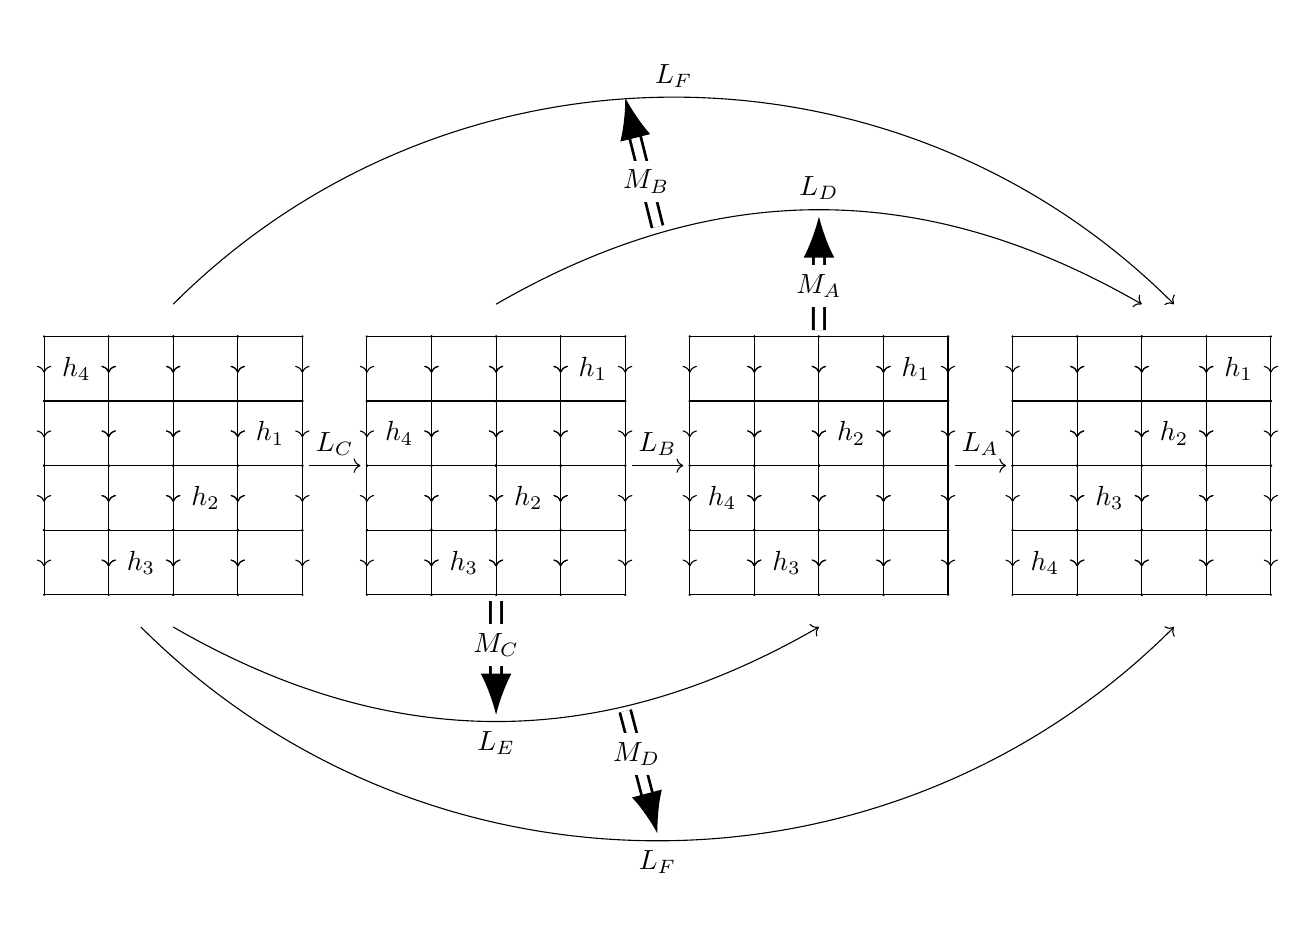
\begin{tikzpicture}[scale=0.82]
  \begin{scope}[xshift=0.0cm]
  \draw[->] (4.1,-2) to (4.9,-2);
      \node at (4.5,-2) [above]{$L_C$};
  	\begin{scope}[xshift=0.0cm]
	      \draw (0,0) to node[sloped] {\tikz{\draw[->](0,0)--(0.1,0);}} (0,-1);
	      \draw (1,0) to node[sloped] {\tikz{\draw[->](0,0)--(0.1,0);}} (1,-1);
	      \draw (0,0) to node[sloped] {\tikz{\draw[-](0,0)--(0.1,0);}} (1,0);
	      \draw (0,-1) to node  {\tikz{\draw[-](0,0)--(0.1,0);}} (1,-1);
	      \node at (1/2,-1/2) {$h_4$};
	      \draw (0,0) to node {\tikz{\draw[-](0,0)--(0.1,0);}}(1,0);
	      \draw (0,-1) to node {\tikz{\draw[-](0,0)--(0.1,0);}} (1,-1);
	      \fill[black] (0,0) circle[radius=0.02];
	      \fill[black] (1,0) circle[radius=0.02];
	      \fill[black] (0,-1) circle[radius=0.02];
	      \fill[black] (1,-1) circle[radius=0.02];
	    \begin{scope}[xshift=1.0cm]
	      \draw (0,0) to node[sloped] {\tikz{\draw[->](0,0)--(0.1,0);}} (0,-1);
	      \draw (1,0) to node[sloped] {\tikz{\draw[->](0,0)--(0.1,0);}} (1,-1);
	      \draw (0,0) to node[sloped] {\tikz{\draw[-](0,0)--(0.1,0);}} (1,0);
	      \draw (0,-1) to node  {\tikz{\draw[-](0,0)--(0.1,0);}} (1,-1);
	      \node at (1/2,-1/2) {$$};
	      \draw (0,0) to node {\tikz{\draw[-](0,0)--(0.1,0);}} (1,0);
	      \draw (0,-1) to node {\tikz{\draw[-](0,0)--(0.1,0);}} (1,-1);
	      \fill[black] (0,0) circle[radius=0.02];
	      \fill[black] (1,0) circle[radius=0.02];
	      \fill[black] (0,-1) circle[radius=0.02];
	      \fill[black] (1,-1) circle[radius=0.02];
	    \end{scope}
	    	 \begin{scope}[xshift=2.0cm]
	      \draw (0,0) to node[sloped] {\tikz{\draw[->](0,0)--(0.1,0);}} (0,-1);
	      \draw (1,0) to node[sloped] {\tikz{\draw[->](0,0)--(0.1,0);}} (1,-1);
	      \draw (0,0) to node[sloped] {\tikz{\draw[-](0,0)--(0.1,0);}} (1,0);
	      \draw (0,-1) to node  {\tikz{\draw[-](0,0)--(0.1,0);}} (1,-1);
	      \node at (1/2,-1/2) {$$};
	      \draw (0,0) to node {\tikz{\draw[-](0,0)--(0.1,0);}} (1,0);
	      \draw (0,-1) to node {\tikz{\draw[-](0,0)--(0.1,0);}} (1,-1);
	      \fill[black] (0,0) circle[radius=0.02];
	      \fill[black] (1,0) circle[radius=0.02];
	      \fill[black] (0,-1) circle[radius=0.02];
	      \fill[black] (1,-1) circle[radius=0.02];
	    \end{scope}
	     \begin{scope}[xshift=3.0cm]
	      \draw (0,0) to node[sloped] {\tikz{\draw[->](0,0)--(0.1,0);}} (0,-1);
	      \draw (1,0) to node[sloped] {\tikz{\draw[->](0,0)--(0.1,0);}} (1,-1);
	      \draw (0,0) to node[sloped] {\tikz{\draw[-](0,0)--(0.1,0);}} (1,0);
	      \draw (0,-1) to node  {\tikz{\draw[-](0,0)--(0.1,0);}} (1,-1);
	      \node at (1/2,-1/2) {$$};
	      \draw (0,0) to node {\tikz{\draw[-](0,0)--(0.1,0);}} (1,0);
	      \draw (0,-1) to node {\tikz{\draw[-](0,0)--(0.1,0);}} (1,-1);
	      \fill[black] (0,0) circle[radius=0.02];
	      \fill[black] (1,0) circle[radius=0.02];
	      \fill[black] (0,-1) circle[radius=0.02];
	      \fill[black] (1,-1) circle[radius=0.02];
	    \end{scope}
	     \end{scope}
	     %%%%%%%%%%%%%%%%%%%%%
	\begin{scope}[yshift=-1.0cm]
  	\begin{scope}[xshift=0.0cm]
	      \draw (0,0) to node[sloped] {\tikz{\draw[->](0,0)--(0.1,0);}} (0,-1);
	      \draw (1,0) to node[sloped] {\tikz{\draw[->](0,0)--(0.1,0);}} (1,-1);
	      \draw (0,0) to node[sloped] {\tikz{\draw[-](0,0)--(0.1,0);}} (1,0);
	      \draw (0,-1) to node  {\tikz{\draw[-](0,0)--(0.1,0);}} (1,-1);
	      \node at (1/2,-1/2) {$$};
	      \draw (0,0) to node {\tikz{\draw[-](0,0)--(0.1,0);}}(1,0);
	      \draw (0,-1) to node {\tikz{\draw[-](0,0)--(0.1,0);}} (1,-1);
	      \fill[black] (0,0) circle[radius=0.02];
	      \fill[black] (1,0) circle[radius=0.02];
	      \fill[black] (0,-1) circle[radius=0.02];
	      \fill[black] (1,-1) circle[radius=0.02];
	      \end{scope}
	    \begin{scope}[xshift=1.0cm]
	      \draw (0,0) to node[sloped] {\tikz{\draw[->](0,0)--(0.1,0);}} (0,-1);
	      \draw (1,0) to node[sloped] {\tikz{\draw[->](0,0)--(0.1,0);}} (1,-1);
	      \draw (0,0) to node[sloped] {\tikz{\draw[-](0,0)--(0.1,0);}} (1,0);
	      \draw (0,-1) to node  {\tikz{\draw[-](0,0)--(0.1,0);}} (1,-1);
	      \node at (1/2,-1/2) {$$};
	      \draw (0,0) to node {\tikz{\draw[-](0,0)--(0.1,0);}} (1,0);
	      \draw (0,-1) to node {\tikz{\draw[-](0,0)--(0.1,0);}} (1,-1);
	      \fill[black] (0,0) circle[radius=0.02];
	      \fill[black] (1,0) circle[radius=0.02];
	      \fill[black] (0,-1) circle[radius=0.02];
	      \fill[black] (1,-1) circle[radius=0.02];
	    \end{scope}
	    	 \begin{scope}[xshift=2.0cm]
	      \draw (0,0) to node[sloped] {\tikz{\draw[->](0,0)--(0.1,0);}} (0,-1);
	      \draw (1,0) to node[sloped] {\tikz{\draw[->](0,0)--(0.1,0);}} (1,-1);
	      \draw (0,0) to node[sloped] {\tikz{\draw[-](0,0)--(0.1,0);}} (1,0);
	      \draw (0,-1) to node  {\tikz{\draw[-](0,0)--(0.1,0);}} (1,-1);
	      \node at (1/2,-1/2) {$$};
	      \draw (0,0) to node {\tikz{\draw[-](0,0)--(0.1,0);}} (1,0);
	      \draw (0,-1) to node {\tikz{\draw[-](0,0)--(0.1,0);}} (1,-1);
	      \fill[black] (0,0) circle[radius=0.02];
	      \fill[black] (1,0) circle[radius=0.02];
	      \fill[black] (0,-1) circle[radius=0.02];
	      \fill[black] (1,-1) circle[radius=0.02];
	    \end{scope}
	     \begin{scope}[xshift=3.0cm]
	      \draw (0,0) to node[sloped] {\tikz{\draw[->](0,0)--(0.1,0);}} (0,-1);
	      \draw (1,0) to node[sloped] {\tikz{\draw[->](0,0)--(0.1,0);}} (1,-1);
	      \draw (0,0) to node[sloped] {\tikz{\draw[-](0,0)--(0.1,0);}} (1,0);
	      \draw (0,-1) to node  {\tikz{\draw[-](0,0)--(0.1,0);}} (1,-1);
	      \node at (1/2,-1/2) {$h_1$};
	      \draw (0,0) to node {\tikz{\draw[-](0,0)--(0.1,0);}} (1,0);
	      \draw (0,-1) to node {\tikz{\draw[-](0,0)--(0.1,0);}} (1,-1);
	      \fill[black] (0,0) circle[radius=0.02];
	      \fill[black] (1,0) circle[radius=0.02];
	      \fill[black] (0,-1) circle[radius=0.02];
	      \fill[black] (1,-1) circle[radius=0.02];
	    \end{scope}
	     \end{scope}
	       %%%%%%%%%%%%%%%%%%%%%
	     \begin{scope}[yshift=-2.0cm]
  	\begin{scope}[xshift=0.0cm]
	      \draw (0,0) to node[sloped] {\tikz{\draw[->](0,0)--(0.1,0);}} (0,-1);
	      \draw (1,0) to node[sloped] {\tikz{\draw[->](0,0)--(0.1,0);}} (1,-1);
	      \draw (0,0) to node[sloped] {\tikz{\draw[-](0,0)--(0.1,0);}} (1,0);
	      \draw (0,-1) to node  {\tikz{\draw[-](0,0)--(0.1,0);}} (1,-1);
	      \node at (1/2,-1/2) {$$};
	      \draw (0,0) to node {\tikz{\draw[-](0,0)--(0.1,0);}}(1,0);
	      \draw (0,-1) to node {\tikz{\draw[-](0,0)--(0.1,0);}} (1,-1);
	      \fill[black] (0,0) circle[radius=0.02];
	      \fill[black] (1,0) circle[radius=0.02];
	      \fill[black] (0,-1) circle[radius=0.02];
	      \fill[black] (1,-1) circle[radius=0.02];
	      \end{scope}
	    \begin{scope}[xshift=1.0cm]
	      \draw (0,0) to node[sloped] {\tikz{\draw[->](0,0)--(0.1,0);}} (0,-1);
	      \draw (1,0) to node[sloped] {\tikz{\draw[->](0,0)--(0.1,0);}} (1,-1);
	      \draw (0,0) to node[sloped] {\tikz{\draw[-](0,0)--(0.1,0);}} (1,0);
	      \draw (0,-1) to node  {\tikz{\draw[-](0,0)--(0.1,0);}} (1,-1);
	      \node at (1/2,-1/2) {$$};
	      \draw (0,0) to node {\tikz{\draw[-](0,0)--(0.1,0);}} (1,0);
	      \draw (0,-1) to node {\tikz{\draw[-](0,0)--(0.1,0);}} (1,-1);
	      \fill[black] (0,0) circle[radius=0.02];
	      \fill[black] (1,0) circle[radius=0.02];
	      \fill[black] (0,-1) circle[radius=0.02];
	      \fill[black] (1,-1) circle[radius=0.02];
	    \end{scope}
	    	 \begin{scope}[xshift=2.0cm]
	      \draw (0,0) to node[sloped] {\tikz{\draw[->](0,0)--(0.1,0);}} (0,-1);
	      \draw (1,0) to node[sloped] {\tikz{\draw[->](0,0)--(0.1,0);}} (1,-1);
	      \draw (0,0) to node[sloped] {\tikz{\draw[-](0,0)--(0.1,0);}} (1,0);
	      \draw (0,-1) to node  {\tikz{\draw[-](0,0)--(0.1,0);}} (1,-1);
	      \node at (1/2,-1/2) {$h_2$};
	      \draw (0,0) to node {\tikz{\draw[-](0,0)--(0.1,0);}} (1,0);
	      \draw (0,-1) to node {\tikz{\draw[-](0,0)--(0.1,0);}} (1,-1);
	      \fill[black] (0,0) circle[radius=0.02];
	      \fill[black] (1,0) circle[radius=0.02];
	      \fill[black] (0,-1) circle[radius=0.02];
	      \fill[black] (1,-1) circle[radius=0.02];
	    \end{scope}
	     \begin{scope}[xshift=3.0cm]
	      \draw (0,0) to node[sloped] {\tikz{\draw[->](0,0)--(0.1,0);}} (0,-1);
	      \draw (1,0) to node[sloped] {\tikz{\draw[->](0,0)--(0.1,0);}} (1,-1);
	      \draw (0,0) to node[sloped] {\tikz{\draw[-](0,0)--(0.1,0);}} (1,0);
	      \draw (0,-1) to node  {\tikz{\draw[-](0,0)--(0.1,0);}} (1,-1);
	      \node at (1/2,-1/2) {$$};
	      \draw (0,0) to node {\tikz{\draw[-](0,0)--(0.1,0);}} (1,0);
	      \draw (0,-1) to node {\tikz{\draw[-](0,0)--(0.1,0);}} (1,-1);
	      \fill[black] (0,0) circle[radius=0.02];
	      \fill[black] (1,0) circle[radius=0.02];
	      \fill[black] (0,-1) circle[radius=0.02];
	      \fill[black] (1,-1) circle[radius=0.02];
	    \end{scope}
	     \end{scope}
	       %%%%%%%%%%%%%%%%%%%%%
    \begin{scope}[yshift=-3.0cm]
  	\begin{scope}[xshift=0.0cm]
	      \draw (0,0) to node[sloped] {\tikz{\draw[->](0,0)--(0.1,0);}} (0,-1);
	      \draw (1,0) to node[sloped] {\tikz{\draw[->](0,0)--(0.1,0);}} (1,-1);
	      \draw (0,0) to node[sloped] {\tikz{\draw[-](0,0)--(0.1,0);}} (1,0);
	      \draw (0,-1) to node  {\tikz{\draw[-](0,0)--(0.1,0);}} (1,-1);
	      \node at (1/2,-1/2) {$$};
	      \draw (0,0) to node {\tikz{\draw[-](0,0)--(0.1,0);}}(1,0);
	      \draw (0,-1) to node {\tikz{\draw[-](0,0)--(0.1,0);}} (1,-1);
	      \fill[black] (0,0) circle[radius=0.02];
	      \fill[black] (1,0) circle[radius=0.02];
	      \fill[black] (0,-1) circle[radius=0.02];
	      \fill[black] (1,-1) circle[radius=0.02];
	      \end{scope}
	    \begin{scope}[xshift=1.0cm]
	      \draw (0,0) to node[sloped] {\tikz{\draw[->](0,0)--(0.1,0);}} (0,-1);
	      \draw (1,0) to node[sloped] {\tikz{\draw[->](0,0)--(0.1,0);}} (1,-1);
	      \draw (0,0) to node[sloped] {\tikz{\draw[-](0,0)--(0.1,0);}} (1,0);
	      \draw (0,-1) to node  {\tikz{\draw[-](0,0)--(0.1,0);}} (1,-1);
	      \node at (1/2,-1/2) {$h_3$};
	      \draw (0,0) to node {\tikz{\draw[-](0,0)--(0.1,0);}} (1,0);
	      \draw (0,-1) to node {\tikz{\draw[-](0,0)--(0.1,0);}} (1,-1);
	      \fill[black] (0,0) circle[radius=0.02];
	      \fill[black] (1,0) circle[radius=0.02];
	      \fill[black] (0,-1) circle[radius=0.02];
	      \fill[black] (1,-1) circle[radius=0.02];
	    \end{scope}
	    	 \begin{scope}[xshift=2.0cm]
	      \draw (0,0) to node[sloped] {\tikz{\draw[->](0,0)--(0.1,0);}} (0,-1);
	      \draw (1,0) to node[sloped] {\tikz{\draw[->](0,0)--(0.1,0);}} (1,-1);
	      \draw (0,0) to node[sloped] {\tikz{\draw[-](0,0)--(0.1,0);}} (1,0);
	      \draw (0,-1) to node  {\tikz{\draw[-](0,0)--(0.1,0);}} (1,-1);
	      \node at (1/2,-1/2) {$$};
	      \draw (0,0) to node {\tikz{\draw[-](0,0)--(0.1,0);}} (1,0);
	      \draw (0,-1) to node {\tikz{\draw[-](0,0)--(0.1,0);}} (1,-1);
	      \fill[black] (0,0) circle[radius=0.02];
	      \fill[black] (1,0) circle[radius=0.02];
	      \fill[black] (0,-1) circle[radius=0.02];
	      \fill[black] (1,-1) circle[radius=0.02];
	    \end{scope}
	     \begin{scope}[xshift=3.0cm]
	      \draw (0,0) to node[sloped] {\tikz{\draw[->](0,0)--(0.1,0);}} (0,-1);
	      \draw (1,0) to node[sloped] {\tikz{\draw[->](0,0)--(0.1,0);}} (1,-1);
	      \draw (0,0) to node[sloped] {\tikz{\draw[-](0,0)--(0.1,0);}} (1,0);
	      \draw (0,-1) to node  {\tikz{\draw[-](0,0)--(0.1,0);}} (1,-1);
	      \node at (1/2,-1/2) {$$};
	      \draw (0,0) to node {\tikz{\draw[-](0,0)--(0.1,0);}} (1,0);
	      \draw (0,-1) to node {\tikz{\draw[-](0,0)--(0.1,0);}} (1,-1);
	      \fill[black] (0,0) circle[radius=0.02];
	      \fill[black] (1,0) circle[radius=0.02];
	      \fill[black] (0,-1) circle[radius=0.02];
	      \fill[black] (1,-1) circle[radius=0.02];
	    \end{scope}
	     \end{scope}
	      \end{scope}
	     %%%%%%%%%%%%%%%%
	     %%%%%%%%%%%%%%%%
	     %%%%%%%%%%%%%%%
	     %%%%%%%%%%%%%%%%
	       \begin{scope}[xshift=5.0cm]
  \draw[->] (4.1,-2) to (4.9,-2);
      \node at (4.5,-2) [above]{$L_B$};
  	\begin{scope}[xshift=0.0cm]
	      \draw (0,0) to node[sloped] {\tikz{\draw[->](0,0)--(0.1,0);}} (0,-1);
	      \draw (1,0) to node[sloped] {\tikz{\draw[->](0,0)--(0.1,0);}} (1,-1);
	      \draw (0,0) to node[sloped] {\tikz{\draw[-](0,0)--(0.1,0);}} (1,0);
	      \draw (0,-1) to node  {\tikz{\draw[-](0,0)--(0.1,0);}} (1,-1);
	      \node at (1/2,-1/2) {$$};
	      \draw (0,0) to node {\tikz{\draw[-](0,0)--(0.1,0);}}(1,0);
	      \draw (0,-1) to node {\tikz{\draw[-](0,0)--(0.1,0);}} (1,-1);
	      \fill[black] (0,0) circle[radius=0.02];
	      \fill[black] (1,0) circle[radius=0.02];
	      \fill[black] (0,-1) circle[radius=0.02];
	      \fill[black] (1,-1) circle[radius=0.02];
	    \begin{scope}[xshift=1.0cm]
	      \draw (0,0) to node[sloped] {\tikz{\draw[->](0,0)--(0.1,0);}} (0,-1);
	      \draw (1,0) to node[sloped] {\tikz{\draw[->](0,0)--(0.1,0);}} (1,-1);
	      \draw (0,0) to node[sloped] {\tikz{\draw[-](0,0)--(0.1,0);}} (1,0);
	      \draw (0,-1) to node  {\tikz{\draw[-](0,0)--(0.1,0);}} (1,-1);
	      \node at (1/2,-1/2) {$$};
	      \draw (0,0) to node {\tikz{\draw[-](0,0)--(0.1,0);}} (1,0);
	      \draw (0,-1) to node {\tikz{\draw[-](0,0)--(0.1,0);}} (1,-1);
	      \fill[black] (0,0) circle[radius=0.02];
	      \fill[black] (1,0) circle[radius=0.02];
	      \fill[black] (0,-1) circle[radius=0.02];
	      \fill[black] (1,-1) circle[radius=0.02];
	    \end{scope}
	    	 \begin{scope}[xshift=2.0cm]
	      \draw (0,0) to node[sloped] {\tikz{\draw[->](0,0)--(0.1,0);}} (0,-1);
	      \draw (1,0) to node[sloped] {\tikz{\draw[->](0,0)--(0.1,0);}} (1,-1);
	      \draw (0,0) to node[sloped] {\tikz{\draw[-](0,0)--(0.1,0);}} (1,0);
	      \draw (0,-1) to node  {\tikz{\draw[-](0,0)--(0.1,0);}} (1,-1);
	      \node at (1/2,-1/2) {$$};
	      \draw (0,0) to node {\tikz{\draw[-](0,0)--(0.1,0);}} (1,0);
	      \draw (0,-1) to node {\tikz{\draw[-](0,0)--(0.1,0);}} (1,-1);
	      \fill[black] (0,0) circle[radius=0.02];
	      \fill[black] (1,0) circle[radius=0.02];
	      \fill[black] (0,-1) circle[radius=0.02];
	      \fill[black] (1,-1) circle[radius=0.02];
	    \end{scope}
	     \begin{scope}[xshift=3.0cm]
	      \draw (0,0) to node[sloped] {\tikz{\draw[->](0,0)--(0.1,0);}} (0,-1);
	      \draw (1,0) to node[sloped] {\tikz{\draw[->](0,0)--(0.1,0);}} (1,-1);
	      \draw (0,0) to node[sloped] {\tikz{\draw[-](0,0)--(0.1,0);}} (1,0);
	      \draw (0,-1) to node  {\tikz{\draw[-](0,0)--(0.1,0);}} (1,-1);
	      \node at (1/2,-1/2) {$h_1$};
	      \draw (0,0) to node {\tikz{\draw[-](0,0)--(0.1,0);}} (1,0);
	      \draw (0,-1) to node {\tikz{\draw[-](0,0)--(0.1,0);}} (1,-1);
	      \fill[black] (0,0) circle[radius=0.02];
	      \fill[black] (1,0) circle[radius=0.02];
	      \fill[black] (0,-1) circle[radius=0.02];
	      \fill[black] (1,-1) circle[radius=0.02];
	    \end{scope}
	     \end{scope}
	     %%%%%%%%%%%%%%%%%%%%%
	\begin{scope}[yshift=-1.0cm]
  	\begin{scope}[xshift=0.0cm]
	      \draw (0,0) to node[sloped] {\tikz{\draw[->](0,0)--(0.1,0);}} (0,-1);
	      \draw (1,0) to node[sloped] {\tikz{\draw[->](0,0)--(0.1,0);}} (1,-1);
	      \draw (0,0) to node[sloped] {\tikz{\draw[-](0,0)--(0.1,0);}} (1,0);
	      \draw (0,-1) to node  {\tikz{\draw[-](0,0)--(0.1,0);}} (1,-1);
	      \node at (1/2,-1/2) {$h_4$};
	      \draw (0,0) to node {\tikz{\draw[-](0,0)--(0.1,0);}}(1,0);
	      \draw (0,-1) to node {\tikz{\draw[-](0,0)--(0.1,0);}} (1,-1);
	      \fill[black] (0,0) circle[radius=0.02];
	      \fill[black] (1,0) circle[radius=0.02];
	      \fill[black] (0,-1) circle[radius=0.02];
	      \fill[black] (1,-1) circle[radius=0.02];
	      \end{scope}
	    \begin{scope}[xshift=1.0cm]
	      \draw (0,0) to node[sloped] {\tikz{\draw[->](0,0)--(0.1,0);}} (0,-1);
	      \draw (1,0) to node[sloped] {\tikz{\draw[->](0,0)--(0.1,0);}} (1,-1);
	      \draw (0,0) to node[sloped] {\tikz{\draw[-](0,0)--(0.1,0);}} (1,0);
	      \draw (0,-1) to node  {\tikz{\draw[-](0,0)--(0.1,0);}} (1,-1);
	      \node at (1/2,-1/2) {$$};
	      \draw (0,0) to node {\tikz{\draw[-](0,0)--(0.1,0);}} (1,0);
	      \draw (0,-1) to node {\tikz{\draw[-](0,0)--(0.1,0);}} (1,-1);
	      \fill[black] (0,0) circle[radius=0.02];
	      \fill[black] (1,0) circle[radius=0.02];
	      \fill[black] (0,-1) circle[radius=0.02];
	      \fill[black] (1,-1) circle[radius=0.02];
	    \end{scope}
	    	 \begin{scope}[xshift=2.0cm]
	      \draw (0,0) to node[sloped] {\tikz{\draw[->](0,0)--(0.1,0);}} (0,-1);
	      \draw (1,0) to node[sloped] {\tikz{\draw[->](0,0)--(0.1,0);}} (1,-1);
	      \draw (0,0) to node[sloped] {\tikz{\draw[-](0,0)--(0.1,0);}} (1,0);
	      \draw (0,-1) to node  {\tikz{\draw[-](0,0)--(0.1,0);}} (1,-1);
	      \node at (1/2,-1/2) {$$};
	      \draw (0,0) to node {\tikz{\draw[-](0,0)--(0.1,0);}} (1,0);
	      \draw (0,-1) to node {\tikz{\draw[-](0,0)--(0.1,0);}} (1,-1);
	      \fill[black] (0,0) circle[radius=0.02];
	      \fill[black] (1,0) circle[radius=0.02];
	      \fill[black] (0,-1) circle[radius=0.02];
	      \fill[black] (1,-1) circle[radius=0.02];
	    \end{scope}
	     \begin{scope}[xshift=3.0cm]
	      \draw (0,0) to node[sloped] {\tikz{\draw[->](0,0)--(0.1,0);}} (0,-1);
	      \draw (1,0) to node[sloped] {\tikz{\draw[->](0,0)--(0.1,0);}} (1,-1);
	      \draw (0,0) to node[sloped] {\tikz{\draw[-](0,0)--(0.1,0);}} (1,0);
	      \draw (0,-1) to node  {\tikz{\draw[-](0,0)--(0.1,0);}} (1,-1);
	      \node at (1/2,-1/2) {$$};
	      \draw (0,0) to node {\tikz{\draw[-](0,0)--(0.1,0);}} (1,0);
	      \draw (0,-1) to node {\tikz{\draw[-](0,0)--(0.1,0);}} (1,-1);
	      \fill[black] (0,0) circle[radius=0.02];
	      \fill[black] (1,0) circle[radius=0.02];
	      \fill[black] (0,-1) circle[radius=0.02];
	      \fill[black] (1,-1) circle[radius=0.02];
	    \end{scope}
	     \end{scope}
	       %%%%%%%%%%%%%%%%%%%%%
	     \begin{scope}[yshift=-2.0cm]
  	\begin{scope}[xshift=0.0cm]
	      \draw (0,0) to node[sloped] {\tikz{\draw[->](0,0)--(0.1,0);}} (0,-1);
	      \draw (1,0) to node[sloped] {\tikz{\draw[->](0,0)--(0.1,0);}} (1,-1);
	      \draw (0,0) to node[sloped] {\tikz{\draw[-](0,0)--(0.1,0);}} (1,0);
	      \draw (0,-1) to node  {\tikz{\draw[-](0,0)--(0.1,0);}} (1,-1);
	      \node at (1/2,-1/2) {$$};
	      \draw (0,0) to node {\tikz{\draw[-](0,0)--(0.1,0);}}(1,0);
	      \draw (0,-1) to node {\tikz{\draw[-](0,0)--(0.1,0);}} (1,-1);
	      \fill[black] (0,0) circle[radius=0.02];
	      \fill[black] (1,0) circle[radius=0.02];
	      \fill[black] (0,-1) circle[radius=0.02];
	      \fill[black] (1,-1) circle[radius=0.02];
	      \end{scope}
	    \begin{scope}[xshift=1.0cm]
	      \draw (0,0) to node[sloped] {\tikz{\draw[->](0,0)--(0.1,0);}} (0,-1);
	      \draw (1,0) to node[sloped] {\tikz{\draw[->](0,0)--(0.1,0);}} (1,-1);
	      \draw (0,0) to node[sloped] {\tikz{\draw[-](0,0)--(0.1,0);}} (1,0);
	      \draw (0,-1) to node  {\tikz{\draw[-](0,0)--(0.1,0);}} (1,-1);
	      \node at (1/2,-1/2) {$$};
	      \draw (0,0) to node {\tikz{\draw[-](0,0)--(0.1,0);}} (1,0);
	      \draw (0,-1) to node {\tikz{\draw[-](0,0)--(0.1,0);}} (1,-1);
	      \fill[black] (0,0) circle[radius=0.02];
	      \fill[black] (1,0) circle[radius=0.02];
	      \fill[black] (0,-1) circle[radius=0.02];
	      \fill[black] (1,-1) circle[radius=0.02];
	    \end{scope}
	    	 \begin{scope}[xshift=2.0cm]
	      \draw (0,0) to node[sloped] {\tikz{\draw[->](0,0)--(0.1,0);}} (0,-1);
	      \draw (1,0) to node[sloped] {\tikz{\draw[->](0,0)--(0.1,0);}} (1,-1);
	      \draw (0,0) to node[sloped] {\tikz{\draw[-](0,0)--(0.1,0);}} (1,0);
	      \draw (0,-1) to node  {\tikz{\draw[-](0,0)--(0.1,0);}} (1,-1);
	      \node at (1/2,-1/2) {$h_2$};
	      \draw (0,0) to node {\tikz{\draw[-](0,0)--(0.1,0);}} (1,0);
	      \draw (0,-1) to node {\tikz{\draw[-](0,0)--(0.1,0);}} (1,-1);
	      \fill[black] (0,0) circle[radius=0.02];
	      \fill[black] (1,0) circle[radius=0.02];
	      \fill[black] (0,-1) circle[radius=0.02];
	      \fill[black] (1,-1) circle[radius=0.02];
	    \end{scope}
	     \begin{scope}[xshift=3.0cm]
	      \draw (0,0) to node[sloped] {\tikz{\draw[->](0,0)--(0.1,0);}} (0,-1);
	      \draw (1,0) to node[sloped] {\tikz{\draw[->](0,0)--(0.1,0);}} (1,-1);
	      \draw (0,0) to node[sloped] {\tikz{\draw[-](0,0)--(0.1,0);}} (1,0);
	      \draw (0,-1) to node  {\tikz{\draw[-](0,0)--(0.1,0);}} (1,-1);
	      \node at (1/2,-1/2) {$$};
	      \draw (0,0) to node {\tikz{\draw[-](0,0)--(0.1,0);}} (1,0);
	      \draw (0,-1) to node {\tikz{\draw[-](0,0)--(0.1,0);}} (1,-1);
	      \fill[black] (0,0) circle[radius=0.02];
	      \fill[black] (1,0) circle[radius=0.02];
	      \fill[black] (0,-1) circle[radius=0.02];
	      \fill[black] (1,-1) circle[radius=0.02];
	    \end{scope}
	     \end{scope}
	       %%%%%%%%%%%%%%%%%%%%%
    \begin{scope}[yshift=-3.0cm]
  	\begin{scope}[xshift=0.0cm]
	      \draw (0,0) to node[sloped] {\tikz{\draw[->](0,0)--(0.1,0);}} (0,-1);
	      \draw (1,0) to node[sloped] {\tikz{\draw[->](0,0)--(0.1,0);}} (1,-1);
	      \draw (0,0) to node[sloped] {\tikz{\draw[-](0,0)--(0.1,0);}} (1,0);
	      \draw (0,-1) to node  {\tikz{\draw[-](0,0)--(0.1,0);}} (1,-1);
	      \node at (1/2,-1/2) {$$};
	      \draw (0,0) to node {\tikz{\draw[-](0,0)--(0.1,0);}}(1,0);
	      \draw (0,-1) to node {\tikz{\draw[-](0,0)--(0.1,0);}} (1,-1);
	      \fill[black] (0,0) circle[radius=0.02];
	      \fill[black] (1,0) circle[radius=0.02];
	      \fill[black] (0,-1) circle[radius=0.02];
	      \fill[black] (1,-1) circle[radius=0.02];
	      \end{scope}
	    \begin{scope}[xshift=1.0cm]
	      \draw (0,0) to node[sloped] {\tikz{\draw[->](0,0)--(0.1,0);}} (0,-1);
	      \draw (1,0) to node[sloped] {\tikz{\draw[->](0,0)--(0.1,0);}} (1,-1);
	      \draw (0,0) to node[sloped] {\tikz{\draw[-](0,0)--(0.1,0);}} (1,0);
	      \draw (0,-1) to node  {\tikz{\draw[-](0,0)--(0.1,0);}} (1,-1);
	      \node at (1/2,-1/2) {$h_3$};
	      \draw (0,0) to node {\tikz{\draw[-](0,0)--(0.1,0);}} (1,0);
	      \draw (0,-1) to node {\tikz{\draw[-](0,0)--(0.1,0);}} (1,-1);
	      \fill[black] (0,0) circle[radius=0.02];
	      \fill[black] (1,0) circle[radius=0.02];
	      \fill[black] (0,-1) circle[radius=0.02];
	      \fill[black] (1,-1) circle[radius=0.02];
	    \end{scope}
	    	 \begin{scope}[xshift=2.0cm]
	      \draw (0,0) to node[sloped] {\tikz{\draw[->](0,0)--(0.1,0);}} (0,-1);
	      \draw (1,0) to node[sloped] {\tikz{\draw[->](0,0)--(0.1,0);}} (1,-1);
	      \draw (0,0) to node[sloped] {\tikz{\draw[-](0,0)--(0.1,0);}} (1,0);
	      \draw (0,-1) to node  {\tikz{\draw[-](0,0)--(0.1,0);}} (1,-1);
	      \node at (1/2,-1/2) {$$};
	      \draw (0,0) to node {\tikz{\draw[-](0,0)--(0.1,0);}} (1,0);
	      \draw (0,-1) to node {\tikz{\draw[-](0,0)--(0.1,0);}} (1,-1);
	      \fill[black] (0,0) circle[radius=0.02];
	      \fill[black] (1,0) circle[radius=0.02];
	      \fill[black] (0,-1) circle[radius=0.02];
	      \fill[black] (1,-1) circle[radius=0.02];
	    \end{scope}
	     \begin{scope}[xshift=3.0cm]
	      \draw (0,0) to node[sloped] {\tikz{\draw[->](0,0)--(0.1,0);}} (0,-1);
	      \draw (1,0) to node[sloped] {\tikz{\draw[->](0,0)--(0.1,0);}} (1,-1);
	      \draw (0,0) to node[sloped] {\tikz{\draw[-](0,0)--(0.1,0);}} (1,0);
	      \draw (0,-1) to node  {\tikz{\draw[-](0,0)--(0.1,0);}} (1,-1);
	      \node at (1/2,-1/2) {$$};
	      \draw (0,0) to node {\tikz{\draw[-](0,0)--(0.1,0);}} (1,0);
	      \draw (0,-1) to node {\tikz{\draw[-](0,0)--(0.1,0);}} (1,-1);
	      \fill[black] (0,0) circle[radius=0.02];
	      \fill[black] (1,0) circle[radius=0.02];
	      \fill[black] (0,-1) circle[radius=0.02];
	      \fill[black] (1,-1) circle[radius=0.02];
	    \end{scope}
	     \end{scope}
	      \end{scope}
	     %%%%%%%%%%%%%%%%
	     %%%%%%%%%%%%%%%%
	     %%%%%%%%%%%%%%%
	     %%%%%%%%%%%%%%%%
	       \begin{scope}[xshift=10.0cm]
  \draw[->] (4.1,-2) to (4.9,-2);
      \node at (4.5,-2) [above]{$L_A$};
  	\begin{scope}[xshift=0.0cm]
	      \draw (0,0) to node[sloped] {\tikz{\draw[->](0,0)--(0.1,0);}} (0,-1);
	      \draw (1,0) to node[sloped] {\tikz{\draw[->](0,0)--(0.1,0);}} (1,-1);
	      \draw (0,0) to node[sloped] {\tikz{\draw[-](0,0)--(0.1,0);}} (1,0);
	      \draw (0,-1) to node  {\tikz{\draw[-](0,0)--(0.1,0);}} (1,-1);
	      \node at (1/2,-1/2) {$$};
	      \draw (0,0) to node {\tikz{\draw[-](0,0)--(0.1,0);}}(1,0);
	      \draw (0,-1) to node {\tikz{\draw[-](0,0)--(0.1,0);}} (1,-1);
	      \fill[black] (0,0) circle[radius=0.02];
	      \fill[black] (1,0) circle[radius=0.02];
	      \fill[black] (0,-1) circle[radius=0.02];
	      \fill[black] (1,-1) circle[radius=0.02];
	    \begin{scope}[xshift=1.0cm]
	      \draw (0,0) to node[sloped] {\tikz{\draw[->](0,0)--(0.1,0);}} (0,-1);
	      \draw (1,0) to node[sloped] {\tikz{\draw[->](0,0)--(0.1,0);}} (1,-1);
	      \draw (0,0) to node[sloped] {\tikz{\draw[-](0,0)--(0.1,0);}} (1,0);
	      \draw (0,-1) to node  {\tikz{\draw[-](0,0)--(0.1,0);}} (1,-1);
	      \node at (1/2,-1/2) {$$};
	      \draw (0,0) to node {\tikz{\draw[-](0,0)--(0.1,0);}} (1,0);
	      \draw (0,-1) to node {\tikz{\draw[-](0,0)--(0.1,0);}} (1,-1);
	      \fill[black] (0,0) circle[radius=0.02];
	      \fill[black] (1,0) circle[radius=0.02];
	      \fill[black] (0,-1) circle[radius=0.02];
	      \fill[black] (1,-1) circle[radius=0.02];
	    \end{scope}
	    	 \begin{scope}[xshift=2.0cm]
	      \draw (0,0) to node[sloped] {\tikz{\draw[->](0,0)--(0.1,0);}} (0,-1);
	      \draw (1,0) to node[sloped] {\tikz{\draw[->](0,0)--(0.1,0);}} (1,-1);
	      \draw (0,0) to node[sloped] {\tikz{\draw[-](0,0)--(0.1,0);}} (1,0);
	      \draw (0,-1) to node  {\tikz{\draw[-](0,0)--(0.1,0);}} (1,-1);
	      \node at (1/2,-1/2) {$$};
	      \draw (0,0) to node {\tikz{\draw[-](0,0)--(0.1,0);}} (1,0);
	      \draw (0,-1) to node {\tikz{\draw[-](0,0)--(0.1,0);}} (1,-1);
	      \fill[black] (0,0) circle[radius=0.02];
	      \fill[black] (1,0) circle[radius=0.02];
	      \fill[black] (0,-1) circle[radius=0.02];
	      \fill[black] (1,-1) circle[radius=0.02];
	    \end{scope}
	     \begin{scope}[xshift=3.0cm]
	      \draw (0,0) to node[sloped] {\tikz{\draw[->](0,0)--(0.1,0);}} (0,-1);
	      \draw (1,0) to node[sloped] {\tikz{\draw[->](0,0)--(0.1,0);}} (1,-1);
	      \draw (0,0) to node[sloped] {\tikz{\draw[-](0,0)--(0.1,0);}} (1,0);
	      \draw (0,-1) to node  {\tikz{\draw[-](0,0)--(0.1,0);}} (1,-1);
	      \node at (1/2,-1/2) {$h_1$};
	      \draw (0,0) to node {\tikz{\draw[-](0,0)--(0.1,0);}} (1,0);
	      \draw (0,-1) to node {\tikz{\draw[-](0,0)--(0.1,0);}} (1,-1);
	      \fill[black] (0,0) circle[radius=0.02];
	      \fill[black] (1,0) circle[radius=0.02];
	      \fill[black] (0,-1) circle[radius=0.02];
	      \fill[black] (1,-1) circle[radius=0.02];
	    \end{scope}
	     \end{scope}
	     %%%%%%%%%%%%%%%%%%%%%
	\begin{scope}[yshift=-1.0cm]
  	\begin{scope}[xshift=0.0cm]
	      \draw (0,0) to node[sloped] {\tikz{\draw[->](0,0)--(0.1,0);}} (0,-1);
	      \draw (1,0) to node[sloped] {\tikz{\draw[->](0,0)--(0.1,0);}} (1,-1);
	      \draw (0,0) to node[sloped] {\tikz{\draw[-](0,0)--(0.1,0);}} (1,0);
	      \draw (0,-1) to node  {\tikz{\draw[-](0,0)--(0.1,0);}} (1,-1);
	      \node at (1/2,-1/2) {$$};
	      \draw (0,0) to node {\tikz{\draw[-](0,0)--(0.1,0);}}(1,0);
	      \draw (0,-1) to node {\tikz{\draw[-](0,0)--(0.1,0);}} (1,-1);
	      \fill[black] (0,0) circle[radius=0.02];
	      \fill[black] (1,0) circle[radius=0.02];
	      \fill[black] (0,-1) circle[radius=0.02];
	      \fill[black] (1,-1) circle[radius=0.02];
	      \end{scope}
	    \begin{scope}[xshift=1.0cm]
	      \draw (0,0) to node[sloped] {\tikz{\draw[->](0,0)--(0.1,0);}} (0,-1);
	      \draw (1,0) to node[sloped] {\tikz{\draw[->](0,0)--(0.1,0);}} (1,-1);
	      \draw (0,0) to node[sloped] {\tikz{\draw[-](0,0)--(0.1,0);}} (1,0);
	      \draw (0,-1) to node  {\tikz{\draw[-](0,0)--(0.1,0);}} (1,-1);
	      \node at (1/2,-1/2) {$$};
	      \draw (0,0) to node {\tikz{\draw[-](0,0)--(0.1,0);}} (1,0);
	      \draw (0,-1) to node {\tikz{\draw[-](0,0)--(0.1,0);}} (1,-1);
	      \fill[black] (0,0) circle[radius=0.02];
	      \fill[black] (1,0) circle[radius=0.02];
	      \fill[black] (0,-1) circle[radius=0.02];
	      \fill[black] (1,-1) circle[radius=0.02];
	    \end{scope}
	    	 \begin{scope}[xshift=2.0cm]
	      \draw (0,0) to node[sloped] {\tikz{\draw[->](0,0)--(0.1,0);}} (0,-1);
	      \draw (1,0) to node[sloped] {\tikz{\draw[->](0,0)--(0.1,0);}} (1,-1);
	      \draw (0,0) to node[sloped] {\tikz{\draw[-](0,0)--(0.1,0);}} (1,0);
	      \draw (0,-1) to node  {\tikz{\draw[-](0,0)--(0.1,0);}} (1,-1);
	      \node at (1/2,-1/2) {$h_2$};
	      \draw (0,0) to node {\tikz{\draw[-](0,0)--(0.1,0);}} (1,0);
	      \draw (0,-1) to node {\tikz{\draw[-](0,0)--(0.1,0);}} (1,-1);
	      \fill[black] (0,0) circle[radius=0.02];
	      \fill[black] (1,0) circle[radius=0.02];
	      \fill[black] (0,-1) circle[radius=0.02];
	      \fill[black] (1,-1) circle[radius=0.02];
	    \end{scope}
	     \begin{scope}[xshift=3.0cm]
	      \draw (0,0) to node[sloped] {\tikz{\draw[->](0,0)--(0.1,0);}} (0,-1);
	      \draw (1,0) to node[sloped] {\tikz{\draw[->](0,0)--(0.1,0);}} (1,-1);
	      \draw (0,0) to node[sloped] {\tikz{\draw[-](0,0)--(0.1,0);}} (1,0);
	      \draw (0,-1) to node  {\tikz{\draw[-](0,0)--(0.1,0);}} (1,-1);
	      \node at (1/2,-1/2) {$$};
	      \draw (0,0) to node {\tikz{\draw[-](0,0)--(0.1,0);}} (1,0);
	      \draw (0,-1) to node {\tikz{\draw[-](0,0)--(0.1,0);}} (1,-1);
	      \fill[black] (0,0) circle[radius=0.02];
	      \fill[black] (1,0) circle[radius=0.02];
	      \fill[black] (0,-1) circle[radius=0.02];
	      \fill[black] (1,-1) circle[radius=0.02];
	    \end{scope}
	     \end{scope}
	       %%%%%%%%%%%%%%%%%%%%%
	     \begin{scope}[yshift=-2.0cm]
  	\begin{scope}[xshift=0.0cm]
	      \draw (0,0) to node[sloped] {\tikz{\draw[->](0,0)--(0.1,0);}} (0,-1);
	      \draw (1,0) to node[sloped] {\tikz{\draw[->](0,0)--(0.1,0);}} (1,-1);
	      \draw (0,0) to node[sloped] {\tikz{\draw[-](0,0)--(0.1,0);}} (1,0);
	      \draw (0,-1) to node  {\tikz{\draw[-](0,0)--(0.1,0);}} (1,-1);
	      \node at (1/2,-1/2) {$h_4$};
	      \draw (0,0) to node {\tikz{\draw[-](0,0)--(0.1,0);}}(1,0);
	      \draw (0,-1) to node {\tikz{\draw[-](0,0)--(0.1,0);}} (1,-1);
	      \fill[black] (0,0) circle[radius=0.02];
	      \fill[black] (1,0) circle[radius=0.02];
	      \fill[black] (0,-1) circle[radius=0.02];
	      \fill[black] (1,-1) circle[radius=0.02];
	      \end{scope}
	    \begin{scope}[xshift=1.0cm]
	      \draw (0,0) to node[sloped] {\tikz{\draw[->](0,0)--(0.1,0);}} (0,-1);
	      \draw (1,0) to node[sloped] {\tikz{\draw[->](0,0)--(0.1,0);}} (1,-1);
	      \draw (0,0) to node[sloped] {\tikz{\draw[-](0,0)--(0.1,0);}} (1,0);
	      \draw (0,-1) to node  {\tikz{\draw[-](0,0)--(0.1,0);}} (1,-1);
	      \node at (1/2,-1/2) {$$};
	      \draw (0,0) to node {\tikz{\draw[-](0,0)--(0.1,0);}} (1,0);
	      \draw (0,-1) to node {\tikz{\draw[-](0,0)--(0.1,0);}} (1,-1);
	      \fill[black] (0,0) circle[radius=0.02];
	      \fill[black] (1,0) circle[radius=0.02];
	      \fill[black] (0,-1) circle[radius=0.02];
	      \fill[black] (1,-1) circle[radius=0.02];
	    \end{scope}
	    	 \begin{scope}[xshift=2.0cm]
	      \draw (0,0) to node[sloped] {\tikz{\draw[->](0,0)--(0.1,0);}} (0,-1);
	      \draw (1,0) to node[sloped] {\tikz{\draw[->](0,0)--(0.1,0);}} (1,-1);
	      \draw (0,0) to node[sloped] {\tikz{\draw[-](0,0)--(0.1,0);}} (1,0);
	      \draw (0,-1) to node  {\tikz{\draw[-](0,0)--(0.1,0);}} (1,-1);
	      \node at (1/2,-1/2) {$$};
	      \draw (0,0) to node {\tikz{\draw[-](0,0)--(0.1,0);}} (1,0);
	      \draw (0,-1) to node {\tikz{\draw[-](0,0)--(0.1,0);}} (1,-1);
	      \fill[black] (0,0) circle[radius=0.02];
	      \fill[black] (1,0) circle[radius=0.02];
	      \fill[black] (0,-1) circle[radius=0.02];
	      \fill[black] (1,-1) circle[radius=0.02];
	    \end{scope}
	     \begin{scope}[xshift=3.0cm]
	      \draw (0,0) to node[sloped] {\tikz{\draw[->](0,0)--(0.1,0);}} (0,-1);
	      \draw (1,0) to node[sloped] {\tikz{\draw[->](0,0)--(0.1,0);}} (1,-1);
	      \draw (0,0) to node[sloped] {\tikz{\draw[-](0,0)--(0.1,0);}} (1,0);
	      \draw (0,-1) to node  {\tikz{\draw[-](0,0)--(0.1,0);}} (1,-1);
	      \node at (1/2,-1/2) {$$};
	      \draw (0,0) to node {\tikz{\draw[-](0,0)--(0.1,0);}} (1,0);
	      \draw (0,-1) to node {\tikz{\draw[-](0,0)--(0.1,0);}} (1,-1);
	      \fill[black] (0,0) circle[radius=0.02];
	      \fill[black] (1,0) circle[radius=0.02];
	      \fill[black] (0,-1) circle[radius=0.02];
	      \fill[black] (1,-1) circle[radius=0.02];
	    \end{scope}
	     \end{scope}
	       %%%%%%%%%%%%%%%%%%%%%
    \begin{scope}[yshift=-3.0cm]
  	\begin{scope}[xshift=0.0cm]
	      \draw (0,0) to node[sloped] {\tikz{\draw[->](0,0)--(0.1,0);}} (0,-1);
	      \draw (1,0) to node[sloped] {\tikz{\draw[->](0,0)--(0.1,0);}} (1,-1);
	      \draw (0,0) to node[sloped] {\tikz{\draw[-](0,0)--(0.1,0);}} (1,0);
	      \draw (0,-1) to node  {\tikz{\draw[-](0,0)--(0.1,0);}} (1,-1);
	      \node at (1/2,-1/2) {$$};
	      \draw (0,0) to node {\tikz{\draw[-](0,0)--(0.1,0);}}(1,0);
	      \draw (0,-1) to node {\tikz{\draw[-](0,0)--(0.1,0);}} (1,-1);
	      \fill[black] (0,0) circle[radius=0.02];
	      \fill[black] (1,0) circle[radius=0.02];
	      \fill[black] (0,-1) circle[radius=0.02];
	      \fill[black] (1,-1) circle[radius=0.02];
	      \end{scope}
	    \begin{scope}[xshift=1.0cm]
	      \draw (0,0) to node[sloped] {\tikz{\draw[->](0,0)--(0.1,0);}} (0,-1);
	      \draw (1,0) to node[sloped] {\tikz{\draw[->](0,0)--(0.1,0);}} (1,-1);
	      \draw (0,0) to node[sloped] {\tikz{\draw[-](0,0)--(0.1,0);}} (1,0);
	      \draw (0,-1) to node  {\tikz{\draw[-](0,0)--(0.1,0);}} (1,-1);
	      \node at (1/2,-1/2) {$h_3$};
	      \draw (0,0) to node {\tikz{\draw[-](0,0)--(0.1,0);}} (1,0);
	      \draw (0,-1) to node {\tikz{\draw[-](0,0)--(0.1,0);}} (1,-1);
	      \fill[black] (0,0) circle[radius=0.02];
	      \fill[black] (1,0) circle[radius=0.02];
	      \fill[black] (0,-1) circle[radius=0.02];
	      \fill[black] (1,-1) circle[radius=0.02];
	    \end{scope}
	    	 \begin{scope}[xshift=2.0cm]
	      \draw (0,0) to node[sloped] {\tikz{\draw[->](0,0)--(0.1,0);}} (0,-1);
	      \draw (1,0) to node[sloped] {\tikz{\draw[->](0,0)--(0.1,0);}} (1,-1);
	      \draw (0,0) to node[sloped] {\tikz{\draw[-](0,0)--(0.1,0);}} (1,0);
	      \draw (0,-1) to node  {\tikz{\draw[-](0,0)--(0.1,0);}} (1,-1);
	      \node at (1/2,-1/2) {$$};
	      \draw (0,0) to node {\tikz{\draw[-](0,0)--(0.1,0);}} (1,0);
	      \draw (0,-1) to node {\tikz{\draw[-](0,0)--(0.1,0);}} (1,-1);
	      \fill[black] (0,0) circle[radius=0.02];
	      \fill[black] (1,0) circle[radius=0.02];
	      \fill[black] (0,-1) circle[radius=0.02];
	      \fill[black] (1,-1) circle[radius=0.02];
	    \end{scope}
	     \begin{scope}[xshift=3.0cm]
	      \draw (0,0) to node[sloped] {\tikz{\draw[->](0,0)--(0.1,0);}} (0,-1);
	      \draw (1,0) to node[sloped] {\tikz{\draw[->](0,0)--(0.1,0);}} (1,-1);
	      \draw (0,0) to node[sloped] {\tikz{\draw[-](0,0)--(0.1,0);}} (1,0);
	      \draw (0,-1) to node  {\tikz{\draw[-](0,0)--(0.1,0);}} (1,-1);
	      \node at (1/2,-1/2) {$$};
	      \draw (0,0) to node {\tikz{\draw[-](0,0)--(0.1,0);}} (1,0);
	      \draw (0,-1) to node {\tikz{\draw[-](0,0)--(0.1,0);}} (1,-1);
	      \fill[black] (0,0) circle[radius=0.02];
	      \fill[black] (1,0) circle[radius=0.02];
	      \fill[black] (0,-1) circle[radius=0.02];
	      \fill[black] (1,-1) circle[radius=0.02];
	    \end{scope}
	     \end{scope}
	      \end{scope}
	     %%%%%%%%%%%%%%%%
	     %%%%%%%%%%%%%%%%
	     %%%%%%%%%%%%%%%
	     %%%%%%%%%%%%%%%%
	       \begin{scope}[xshift=15.0cm]
  	\begin{scope}[xshift=0.0cm]
	      \draw (0,0) to node[sloped] {\tikz{\draw[->](0,0)--(0.1,0);}} (0,-1);
	      \draw (1,0) to node[sloped] {\tikz{\draw[->](0,0)--(0.1,0);}} (1,-1);
	      \draw (0,0) to node[sloped] {\tikz{\draw[-](0,0)--(0.1,0);}} (1,0);
	      \draw (0,-1) to node  {\tikz{\draw[-](0,0)--(0.1,0);}} (1,-1);
	      \node at (1/2,-1/2) {$$};
	      \draw (0,0) to node {\tikz{\draw[-](0,0)--(0.1,0);}}(1,0);
	      \draw (0,-1) to node {\tikz{\draw[-](0,0)--(0.1,0);}} (1,-1);
	      \fill[black] (0,0) circle[radius=0.02];
	      \fill[black] (1,0) circle[radius=0.02];
	      \fill[black] (0,-1) circle[radius=0.02];
	      \fill[black] (1,-1) circle[radius=0.02];
	    \begin{scope}[xshift=1.0cm]
	      \draw (0,0) to node[sloped] {\tikz{\draw[->](0,0)--(0.1,0);}} (0,-1);
	      \draw (1,0) to node[sloped] {\tikz{\draw[->](0,0)--(0.1,0);}} (1,-1);
	      \draw (0,0) to node[sloped] {\tikz{\draw[-](0,0)--(0.1,0);}} (1,0);
	      \draw (0,-1) to node  {\tikz{\draw[-](0,0)--(0.1,0);}} (1,-1);
	      \node at (1/2,-1/2) {$$};
	      \draw (0,0) to node {\tikz{\draw[-](0,0)--(0.1,0);}} (1,0);
	      \draw (0,-1) to node {\tikz{\draw[-](0,0)--(0.1,0);}} (1,-1);
	      \fill[black] (0,0) circle[radius=0.02];
	      \fill[black] (1,0) circle[radius=0.02];
	      \fill[black] (0,-1) circle[radius=0.02];
	      \fill[black] (1,-1) circle[radius=0.02];
	    \end{scope}
	    	 \begin{scope}[xshift=2.0cm]
	      \draw (0,0) to node[sloped] {\tikz{\draw[->](0,0)--(0.1,0);}} (0,-1);
	      \draw (1,0) to node[sloped] {\tikz{\draw[->](0,0)--(0.1,0);}} (1,-1);
	      \draw (0,0) to node[sloped] {\tikz{\draw[-](0,0)--(0.1,0);}} (1,0);
	      \draw (0,-1) to node  {\tikz{\draw[-](0,0)--(0.1,0);}} (1,-1);
	      \node at (1/2,-1/2) {$$};
	      \draw (0,0) to node {\tikz{\draw[-](0,0)--(0.1,0);}} (1,0);
	      \draw (0,-1) to node {\tikz{\draw[-](0,0)--(0.1,0);}} (1,-1);
	      \fill[black] (0,0) circle[radius=0.02];
	      \fill[black] (1,0) circle[radius=0.02];
	      \fill[black] (0,-1) circle[radius=0.02];
	      \fill[black] (1,-1) circle[radius=0.02];
	    \end{scope}
	     \begin{scope}[xshift=3.0cm]
	      \draw (0,0) to node[sloped] {\tikz{\draw[->](0,0)--(0.1,0);}} (0,-1);
	      \draw (1,0) to node[sloped] {\tikz{\draw[->](0,0)--(0.1,0);}} (1,-1);
	      \draw (0,0) to node[sloped] {\tikz{\draw[-](0,0)--(0.1,0);}} (1,0);
	      \draw (0,-1) to node  {\tikz{\draw[-](0,0)--(0.1,0);}} (1,-1);
	      \node at (1/2,-1/2) {$h_1$};
	      \draw (0,0) to node {\tikz{\draw[-](0,0)--(0.1,0);}} (1,0);
	      \draw (0,-1) to node {\tikz{\draw[-](0,0)--(0.1,0);}} (1,-1);
	      \fill[black] (0,0) circle[radius=0.02];
	      \fill[black] (1,0) circle[radius=0.02];
	      \fill[black] (0,-1) circle[radius=0.02];
	      \fill[black] (1,-1) circle[radius=0.02];
	    \end{scope}
	     \end{scope}
	     %%%%%%%%%%%%%%%%%%%%%
	\begin{scope}[yshift=-1.0cm]
  	\begin{scope}[xshift=0.0cm]
	      \draw (0,0) to node[sloped] {\tikz{\draw[->](0,0)--(0.1,0);}} (0,-1);
	      \draw (1,0) to node[sloped] {\tikz{\draw[->](0,0)--(0.1,0);}} (1,-1);
	      \draw (0,0) to node[sloped] {\tikz{\draw[-](0,0)--(0.1,0);}} (1,0);
	      \draw (0,-1) to node  {\tikz{\draw[-](0,0)--(0.1,0);}} (1,-1);
	      \node at (1/2,-1/2) {$$};
	      \draw (0,0) to node {\tikz{\draw[-](0,0)--(0.1,0);}}(1,0);
	      \draw (0,-1) to node {\tikz{\draw[-](0,0)--(0.1,0);}} (1,-1);
	      \fill[black] (0,0) circle[radius=0.02];
	      \fill[black] (1,0) circle[radius=0.02];
	      \fill[black] (0,-1) circle[radius=0.02];
	      \fill[black] (1,-1) circle[radius=0.02];
	      \end{scope}
	    \begin{scope}[xshift=1.0cm]
	      \draw (0,0) to node[sloped] {\tikz{\draw[->](0,0)--(0.1,0);}} (0,-1);
	      \draw (1,0) to node[sloped] {\tikz{\draw[->](0,0)--(0.1,0);}} (1,-1);
	      \draw (0,0) to node[sloped] {\tikz{\draw[-](0,0)--(0.1,0);}} (1,0);
	      \draw (0,-1) to node  {\tikz{\draw[-](0,0)--(0.1,0);}} (1,-1);
	      \node at (1/2,-1/2) {$$};
	      \draw (0,0) to node {\tikz{\draw[-](0,0)--(0.1,0);}} (1,0);
	      \draw (0,-1) to node {\tikz{\draw[-](0,0)--(0.1,0);}} (1,-1);
	      \fill[black] (0,0) circle[radius=0.02];
	      \fill[black] (1,0) circle[radius=0.02];
	      \fill[black] (0,-1) circle[radius=0.02];
	      \fill[black] (1,-1) circle[radius=0.02];
	    \end{scope}
	    	 \begin{scope}[xshift=2.0cm]
	      \draw (0,0) to node[sloped] {\tikz{\draw[->](0,0)--(0.1,0);}} (0,-1);
	      \draw (1,0) to node[sloped] {\tikz{\draw[->](0,0)--(0.1,0);}} (1,-1);
	      \draw (0,0) to node[sloped] {\tikz{\draw[-](0,0)--(0.1,0);}} (1,0);
	      \draw (0,-1) to node  {\tikz{\draw[-](0,0)--(0.1,0);}} (1,-1);
	      \node at (1/2,-1/2) {$h_2$};
	      \draw (0,0) to node {\tikz{\draw[-](0,0)--(0.1,0);}} (1,0);
	      \draw (0,-1) to node {\tikz{\draw[-](0,0)--(0.1,0);}} (1,-1);
	      \fill[black] (0,0) circle[radius=0.02];
	      \fill[black] (1,0) circle[radius=0.02];
	      \fill[black] (0,-1) circle[radius=0.02];
	      \fill[black] (1,-1) circle[radius=0.02];
	    \end{scope}
	     \begin{scope}[xshift=3.0cm]
	      \draw (0,0) to node[sloped] {\tikz{\draw[->](0,0)--(0.1,0);}} (0,-1);
	      \draw (1,0) to node[sloped] {\tikz{\draw[->](0,0)--(0.1,0);}} (1,-1);
	      \draw (0,0) to node[sloped] {\tikz{\draw[-](0,0)--(0.1,0);}} (1,0);
	      \draw (0,-1) to node  {\tikz{\draw[-](0,0)--(0.1,0);}} (1,-1);
	      \node at (1/2,-1/2) {$$};
	      \draw (0,0) to node {\tikz{\draw[-](0,0)--(0.1,0);}} (1,0);
	      \draw (0,-1) to node {\tikz{\draw[-](0,0)--(0.1,0);}} (1,-1);
	      \fill[black] (0,0) circle[radius=0.02];
	      \fill[black] (1,0) circle[radius=0.02];
	      \fill[black] (0,-1) circle[radius=0.02];
	      \fill[black] (1,-1) circle[radius=0.02];
	    \end{scope}
	     \end{scope}
	       %%%%%%%%%%%%%%%%%%%%%
	     \begin{scope}[yshift=-2.0cm]
  	\begin{scope}[xshift=0.0cm]
	      \draw (0,0) to node[sloped] {\tikz{\draw[->](0,0)--(0.1,0);}} (0,-1);
	      \draw (1,0) to node[sloped] {\tikz{\draw[->](0,0)--(0.1,0);}} (1,-1);
	      \draw (0,0) to node[sloped] {\tikz{\draw[-](0,0)--(0.1,0);}} (1,0);
	      \draw (0,-1) to node  {\tikz{\draw[-](0,0)--(0.1,0);}} (1,-1);
	      \node at (1/2,-1/2) {$$};
	      \draw (0,0) to node {\tikz{\draw[-](0,0)--(0.1,0);}}(1,0);
	      \draw (0,-1) to node {\tikz{\draw[-](0,0)--(0.1,0);}} (1,-1);
	      \fill[black] (0,0) circle[radius=0.02];
	      \fill[black] (1,0) circle[radius=0.02];
	      \fill[black] (0,-1) circle[radius=0.02];
	      \fill[black] (1,-1) circle[radius=0.02];
	      \end{scope}
	    \begin{scope}[xshift=1.0cm]
	      \draw (0,0) to node[sloped] {\tikz{\draw[->](0,0)--(0.1,0);}} (0,-1);
	      \draw (1,0) to node[sloped] {\tikz{\draw[->](0,0)--(0.1,0);}} (1,-1);
	      \draw (0,0) to node[sloped] {\tikz{\draw[-](0,0)--(0.1,0);}} (1,0);
	      \draw (0,-1) to node  {\tikz{\draw[-](0,0)--(0.1,0);}} (1,-1);
	      \node at (1/2,-1/2) {$h_3$};
	      \draw (0,0) to node {\tikz{\draw[-](0,0)--(0.1,0);}} (1,0);
	      \draw (0,-1) to node {\tikz{\draw[-](0,0)--(0.1,0);}} (1,-1);
	      \fill[black] (0,0) circle[radius=0.02];
	      \fill[black] (1,0) circle[radius=0.02];
	      \fill[black] (0,-1) circle[radius=0.02];
	      \fill[black] (1,-1) circle[radius=0.02];
	    \end{scope}
	    	 \begin{scope}[xshift=2.0cm]
	      \draw (0,0) to node[sloped] {\tikz{\draw[->](0,0)--(0.1,0);}} (0,-1);
	      \draw (1,0) to node[sloped] {\tikz{\draw[->](0,0)--(0.1,0);}} (1,-1);
	      \draw (0,0) to node[sloped] {\tikz{\draw[-](0,0)--(0.1,0);}} (1,0);
	      \draw (0,-1) to node  {\tikz{\draw[-](0,0)--(0.1,0);}} (1,-1);
	      \node at (1/2,-1/2) {$$};
	      \draw (0,0) to node {\tikz{\draw[-](0,0)--(0.1,0);}} (1,0);
	      \draw (0,-1) to node {\tikz{\draw[-](0,0)--(0.1,0);}} (1,-1);
	      \fill[black] (0,0) circle[radius=0.02];
	      \fill[black] (1,0) circle[radius=0.02];
	      \fill[black] (0,-1) circle[radius=0.02];
	      \fill[black] (1,-1) circle[radius=0.02];
	    \end{scope}
	     \begin{scope}[xshift=3.0cm]
	      \draw (0,0) to node[sloped] {\tikz{\draw[->](0,0)--(0.1,0);}} (0,-1);
	      \draw (1,0) to node[sloped] {\tikz{\draw[->](0,0)--(0.1,0);}} (1,-1);
	      \draw (0,0) to node[sloped] {\tikz{\draw[-](0,0)--(0.1,0);}} (1,0);
	      \draw (0,-1) to node  {\tikz{\draw[-](0,0)--(0.1,0);}} (1,-1);
	      \node at (1/2,-1/2) {$$};
	      \draw (0,0) to node {\tikz{\draw[-](0,0)--(0.1,0);}} (1,0);
	      \draw (0,-1) to node {\tikz{\draw[-](0,0)--(0.1,0);}} (1,-1);
	      \fill[black] (0,0) circle[radius=0.02];
	      \fill[black] (1,0) circle[radius=0.02];
	      \fill[black] (0,-1) circle[radius=0.02];
	      \fill[black] (1,-1) circle[radius=0.02];
	    \end{scope}
	     \end{scope}
	       %%%%%%%%%%%%%%%%%%%%%
    \begin{scope}[yshift=-3.0cm]
  	\begin{scope}[xshift=0.0cm]
	      \draw (0,0) to node[sloped] {\tikz{\draw[->](0,0)--(0.1,0);}} (0,-1);
	      \draw (1,0) to node[sloped] {\tikz{\draw[->](0,0)--(0.1,0);}} (1,-1);
	      \draw (0,0) to node[sloped] {\tikz{\draw[-](0,0)--(0.1,0);}} (1,0);
	      \draw (0,-1) to node  {\tikz{\draw[-](0,0)--(0.1,0);}} (1,-1);
	      \node at (1/2,-1/2) {$h_4$};
	      \draw (0,0) to node {\tikz{\draw[-](0,0)--(0.1,0);}}(1,0);
	      \draw (0,-1) to node {\tikz{\draw[-](0,0)--(0.1,0);}} (1,-1);
	      \fill[black] (0,0) circle[radius=0.02];
	      \fill[black] (1,0) circle[radius=0.02];
	      \fill[black] (0,-1) circle[radius=0.02];
	      \fill[black] (1,-1) circle[radius=0.02];
	      \end{scope}
	    \begin{scope}[xshift=1.0cm]
	      \draw (0,0) to node[sloped] {\tikz{\draw[->](0,0)--(0.1,0);}} (0,-1);
	      \draw (1,0) to node[sloped] {\tikz{\draw[->](0,0)--(0.1,0);}} (1,-1);
	      \draw (0,0) to node[sloped] {\tikz{\draw[-](0,0)--(0.1,0);}} (1,0);
	      \draw (0,-1) to node  {\tikz{\draw[-](0,0)--(0.1,0);}} (1,-1);
	      \node at (1/2,-1/2) {$$};
	      \draw (0,0) to node {\tikz{\draw[-](0,0)--(0.1,0);}} (1,0);
	      \draw (0,-1) to node {\tikz{\draw[-](0,0)--(0.1,0);}} (1,-1);
	      \fill[black] (0,0) circle[radius=0.02];
	      \fill[black] (1,0) circle[radius=0.02];
	      \fill[black] (0,-1) circle[radius=0.02];
	      \fill[black] (1,-1) circle[radius=0.02];
	    \end{scope}
	    	 \begin{scope}[xshift=2.0cm]
	      \draw (0,0) to node[sloped] {\tikz{\draw[->](0,0)--(0.1,0);}} (0,-1);
	      \draw (1,0) to node[sloped] {\tikz{\draw[->](0,0)--(0.1,0);}} (1,-1);
	      \draw (0,0) to node[sloped] {\tikz{\draw[-](0,0)--(0.1,0);}} (1,0);
	      \draw (0,-1) to node  {\tikz{\draw[-](0,0)--(0.1,0);}} (1,-1);
	      \node at (1/2,-1/2) {$$};
	      \draw (0,0) to node {\tikz{\draw[-](0,0)--(0.1,0);}} (1,0);
	      \draw (0,-1) to node {\tikz{\draw[-](0,0)--(0.1,0);}} (1,-1);
	      \fill[black] (0,0) circle[radius=0.02];
	      \fill[black] (1,0) circle[radius=0.02];
	      \fill[black] (0,-1) circle[radius=0.02];
	      \fill[black] (1,-1) circle[radius=0.02];
	    \end{scope}
	     \begin{scope}[xshift=3.0cm]
	      \draw (0,0) to node[sloped] {\tikz{\draw[->](0,0)--(0.1,0);}} (0,-1);
	      \draw (1,0) to node[sloped] {\tikz{\draw[->](0,0)--(0.1,0);}} (1,-1);
	      \draw (0,0) to node[sloped] {\tikz{\draw[-](0,0)--(0.1,0);}} (1,0);
	      \draw (0,-1) to node  {\tikz{\draw[-](0,0)--(0.1,0);}} (1,-1);
	      \node at (1/2,-1/2) {$$};
	      \draw (0,0) to node {\tikz{\draw[-](0,0)--(0.1,0);}} (1,0);
	      \draw (0,-1) to node {\tikz{\draw[-](0,0)--(0.1,0);}} (1,-1);
	      \fill[black] (0,0) circle[radius=0.02];
	      \fill[black] (1,0) circle[radius=0.02];
	      \fill[black] (0,-1) circle[radius=0.02];
	      \fill[black] (1,-1) circle[radius=0.02];
	    \end{scope}
	     \end{scope}
	      \end{scope}
	     \draw[->] (7,0.5) to [out=30,in=150] node[midway] (M1) {} (17,0.5)   ;
	      \node[above] at (M1) {$L_D$};
	     \draw[->] (2,0.5) to [out=45,in=135] node[midway] (M2) {} (17.5,0.5);
	     \node[above] at (M2) {$L_F$};
	     \draw[->] (2,-4.5) to [out=-30,in=-150] node[midway] (M3) {} (12,-4.5);
	     \node[below] at (M3) {$L_E$};
	     \draw[->] (1.5,-4.5) to [out=-45,in=-135] node[midway] (M4) {} (17.5,-4.5);
	     \node[below] at (M4) {$L_F$};
  		\draw [line width=1pt, double distance=3pt, arrows = {-Latex[length=0pt 3 0]}]
        (12.0, 0.1) -- ($(M1) - (0, 0.1)$);
      \node at ($($(12.0, 0.1)!0.5!($(M1) - (0, 0.1)$)$)-(0,0.2)$)  [fill=white]{$M_A$};
      \draw [line width=1pt, double distance=3pt, arrows = {-Latex[length=0pt 3 0]}]
        (7.0, -4.1) -- ($(M3) + (0, 0.1)$);
      \node at ($($(7.0, -4.1)!0.5!($(M3) + (0, 0.1)$)$)+(0,0.2)$)  [fill=white]{$M_C$};
      \draw [line width=1pt, double distance=3pt, arrows = {-Latex[length=0pt 3 0]}]
        (9.5, 1.7) -- (9.0, 3.7);
      \node at ($(9.5, 1.7)!0.35!(9.0, 3.7)$)  [fill=white]{$M_B$};
      \draw [line width=1pt, double distance=3pt, arrows = {-Latex[length=0pt 3 0]}]
        (9, -5.8) -- (9.5, -7.7);
      \node at ($(9, -5.8)!0.35!(9.5, -7.7)$)  [fill=white]{$M_D$};
  \end{tikzpicture}
  }
\end{center}
\caption{Proprety of \ref{rhmnr} of 3-crossed module}
\label{d:rel_of_rhmn}
\end{figure}

In Figure~\ref{d:rel_of_rhmn}, each label form $L_A$ to $L_G$ and from $M_A$ to $M_D$ can be written as in equation~(\ref{eq:drhmnr}).

\begin{equation}
\label{eq:drhmnr}
    \begin{aligned}
L_A &= \act{}\{h_4, h_3\}, \ 
L_B = \act{(\act{\del h_4}h_3)}\{h_4, h_2\} \\
L_C &= \act{\left(\act{\del h_4}(h_3h_2)\right)}\{h_4,h_1\}, \ 
L_D=\act{}\{h_4,h_3, h_2\} \\
L_E &=\act{(\act{\del h_4}h_3)}\{h_4,h_2h_1\}, \ 
L_F =\{h_4,h_3h_2h_1\}\\
M_A &= \act{}\{h_4, h_3, h_2\}', \ 
M_B =\{h_4, h_3 h_2, h_1\}'\\
M_C &= \act{(\act{\del h_4}h_3)}\{h_4,h_2,h_1\}', \ 
M_D = \{h_4,h_3, h_2h_1\}'
\end{aligned}
\end{equation}

This shows that Property~\ref{rhmnr} of a 3-crossed module can be expressed as 
\[
M_B M_A = M_D \act{L_A} M_C.
\]
By examining Figure~\ref{d:rel_of_rhmn}, we see that this property states that the two ways of applying the right-Homanian coincide.

Property~\ref{lrhmnr} of a 3-crossed module can be represented by Figure~\ref{dlrhmnr}.
\begin{figure}[htbp]
\begin{center}
\scalebox{0.7}{
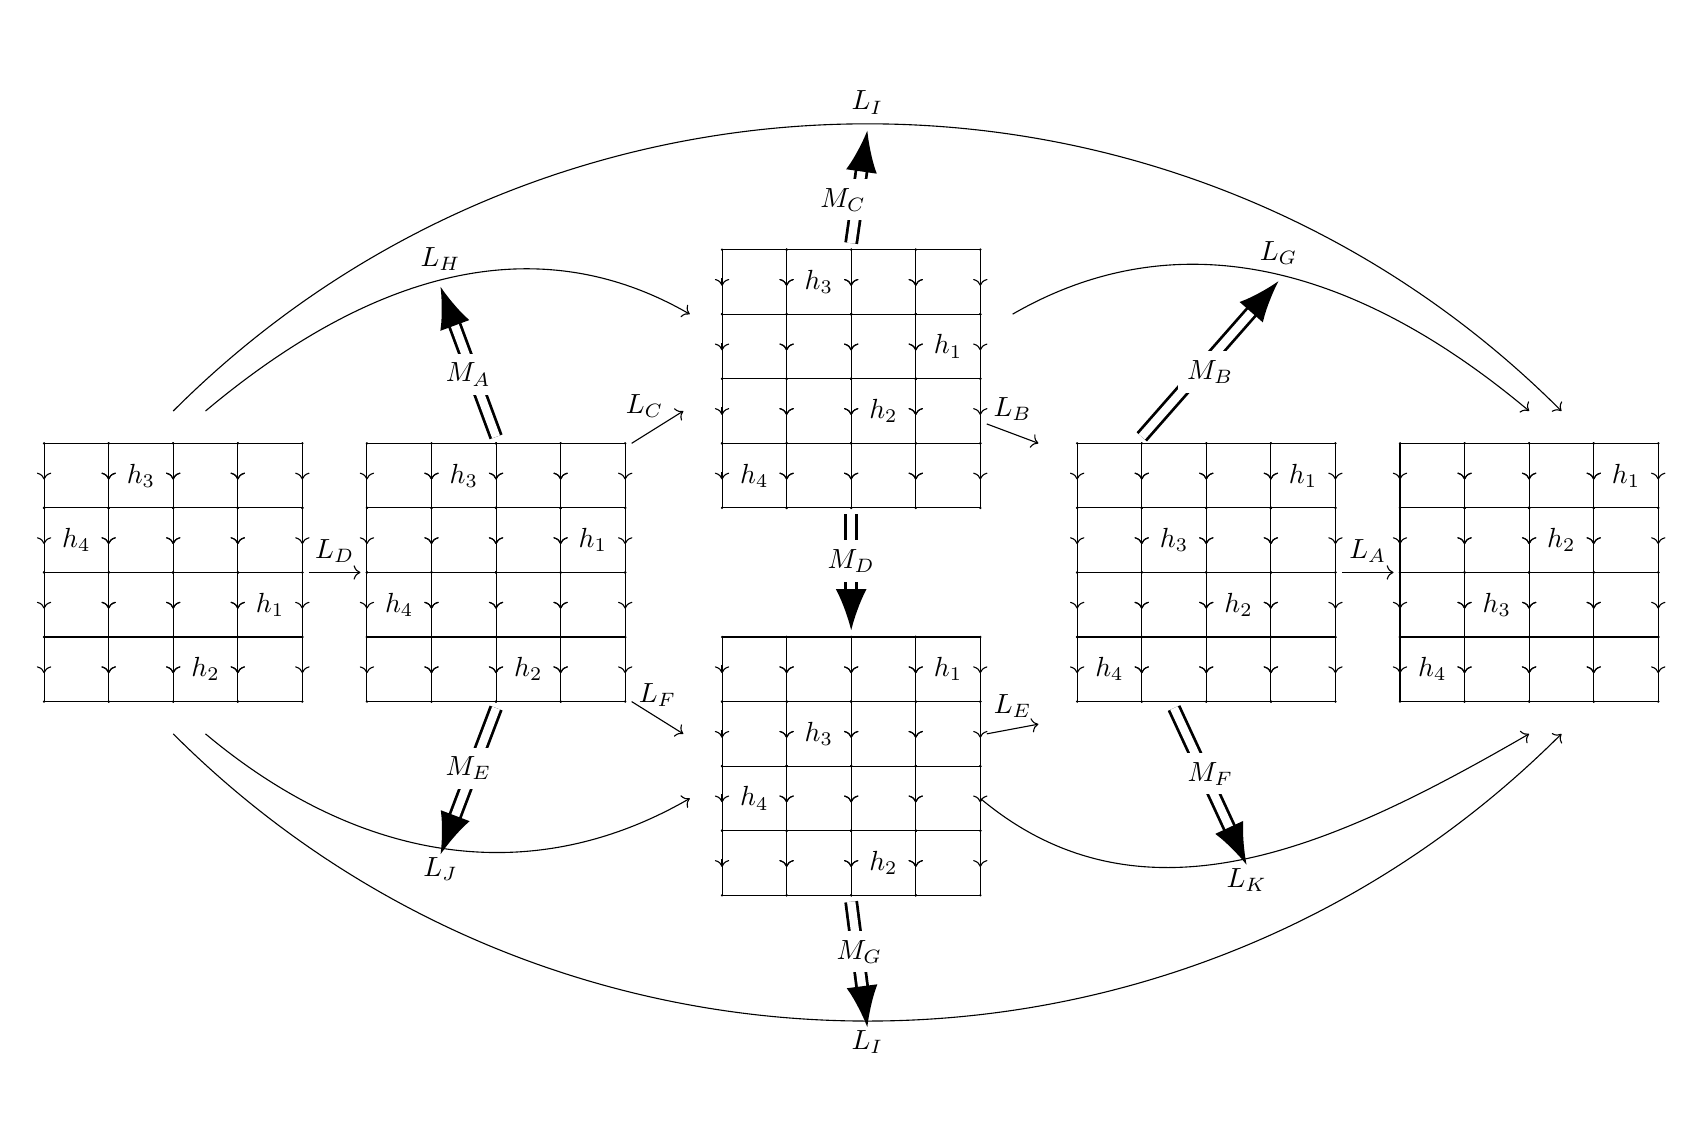
\begin{tikzpicture}[scale=0.82]
%\begin{tikzpicture}[scale=0.82, rotate=90]
  \begin{scope}[xshift=0.0cm]
  \draw[->] (4.1,-2) to (4.9,-2);
      \node at (4.5,-2) [above]{$L_D$};
  	\begin{scope}[xshift=0.0cm]
	      \draw (0,0) to node[sloped] {\tikz{\draw[->](0,0)--(0.1,0);}} (0,-1);
	      \draw (1,0) to node[sloped] {\tikz{\draw[->](0,0)--(0.1,0);}} (1,-1);
	      \draw (0,0) to node[sloped] {\tikz{\draw[-](0,0)--(0.1,0);}} (1,0);
	      \draw (0,-1) to node  {\tikz{\draw[-](0,0)--(0.1,0);}} (1,-1);
	      \node at (1/2,-1/2) {$$};
	      \draw (0,0) to node {\tikz{\draw[-](0,0)--(0.1,0);}}(1,0);
	      \draw (0,-1) to node {\tikz{\draw[-](0,0)--(0.1,0);}} (1,-1);
	      \fill[black] (0,0) circle[radius=0.02];
	      \fill[black] (1,0) circle[radius=0.02];
	      \fill[black] (0,-1) circle[radius=0.02];
	      \fill[black] (1,-1) circle[radius=0.02];
	    \begin{scope}[xshift=1.0cm]
	      \draw (0,0) to node[sloped] {\tikz{\draw[->](0,0)--(0.1,0);}} (0,-1);
	      \draw (1,0) to node[sloped] {\tikz{\draw[->](0,0)--(0.1,0);}} (1,-1);
	      \draw (0,0) to node[sloped] {\tikz{\draw[-](0,0)--(0.1,0);}} (1,0);
	      \draw (0,-1) to node  {\tikz{\draw[-](0,0)--(0.1,0);}} (1,-1);
	      \node at (1/2,-1/2) {$h_3$};
	      \draw (0,0) to node {\tikz{\draw[-](0,0)--(0.1,0);}} (1,0);
	      \draw (0,-1) to node {\tikz{\draw[-](0,0)--(0.1,0);}} (1,-1);
	      \fill[black] (0,0) circle[radius=0.02];
	      \fill[black] (1,0) circle[radius=0.02];
	      \fill[black] (0,-1) circle[radius=0.02];
	      \fill[black] (1,-1) circle[radius=0.02];
	    \end{scope}
	    	 \begin{scope}[xshift=2.0cm]
	      \draw (0,0) to node[sloped] {\tikz{\draw[->](0,0)--(0.1,0);}} (0,-1);
	      \draw (1,0) to node[sloped] {\tikz{\draw[->](0,0)--(0.1,0);}} (1,-1);
	      \draw (0,0) to node[sloped] {\tikz{\draw[-](0,0)--(0.1,0);}} (1,0);
	      \draw (0,-1) to node  {\tikz{\draw[-](0,0)--(0.1,0);}} (1,-1);
	      \node at (1/2,-1/2) {$$};
	      \draw (0,0) to node {\tikz{\draw[-](0,0)--(0.1,0);}} (1,0);
	      \draw (0,-1) to node {\tikz{\draw[-](0,0)--(0.1,0);}} (1,-1);
	      \fill[black] (0,0) circle[radius=0.02];
	      \fill[black] (1,0) circle[radius=0.02];
	      \fill[black] (0,-1) circle[radius=0.02];
	      \fill[black] (1,-1) circle[radius=0.02];
	    \end{scope}
	     \begin{scope}[xshift=3.0cm]
	      \draw (0,0) to node[sloped] {\tikz{\draw[->](0,0)--(0.1,0);}} (0,-1);
	      \draw (1,0) to node[sloped] {\tikz{\draw[->](0,0)--(0.1,0);}} (1,-1);
	      \draw (0,0) to node[sloped] {\tikz{\draw[-](0,0)--(0.1,0);}} (1,0);
	      \draw (0,-1) to node  {\tikz{\draw[-](0,0)--(0.1,0);}} (1,-1);
	      \node at (1/2,-1/2) {$$};
	      \draw (0,0) to node {\tikz{\draw[-](0,0)--(0.1,0);}} (1,0);
	      \draw (0,-1) to node {\tikz{\draw[-](0,0)--(0.1,0);}} (1,-1);
	      \fill[black] (0,0) circle[radius=0.02];
	      \fill[black] (1,0) circle[radius=0.02];
	      \fill[black] (0,-1) circle[radius=0.02];
	      \fill[black] (1,-1) circle[radius=0.02];
	    \end{scope}
	     \end{scope}
	     %%%%%%%%%%%%%%%%%%%%%
	\begin{scope}[yshift=-1.0cm]
  	\begin{scope}[xshift=0.0cm]
	      \draw (0,0) to node[sloped] {\tikz{\draw[->](0,0)--(0.1,0);}} (0,-1);
	      \draw (1,0) to node[sloped] {\tikz{\draw[->](0,0)--(0.1,0);}} (1,-1);
	      \draw (0,0) to node[sloped] {\tikz{\draw[-](0,0)--(0.1,0);}} (1,0);
	      \draw (0,-1) to node  {\tikz{\draw[-](0,0)--(0.1,0);}} (1,-1);
	      \node at (1/2,-1/2) {$h_4$};
	      \draw (0,0) to node {\tikz{\draw[-](0,0)--(0.1,0);}}(1,0);
	      \draw (0,-1) to node {\tikz{\draw[-](0,0)--(0.1,0);}} (1,-1);
	      \fill[black] (0,0) circle[radius=0.02];
	      \fill[black] (1,0) circle[radius=0.02];
	      \fill[black] (0,-1) circle[radius=0.02];
	      \fill[black] (1,-1) circle[radius=0.02];
	      \end{scope}
	    \begin{scope}[xshift=1.0cm]
	      \draw (0,0) to node[sloped] {\tikz{\draw[->](0,0)--(0.1,0);}} (0,-1);
	      \draw (1,0) to node[sloped] {\tikz{\draw[->](0,0)--(0.1,0);}} (1,-1);
	      \draw (0,0) to node[sloped] {\tikz{\draw[-](0,0)--(0.1,0);}} (1,0);
	      \draw (0,-1) to node  {\tikz{\draw[-](0,0)--(0.1,0);}} (1,-1);
	      \node at (1/2,-1/2) {$$};
	      \draw (0,0) to node {\tikz{\draw[-](0,0)--(0.1,0);}} (1,0);
	      \draw (0,-1) to node {\tikz{\draw[-](0,0)--(0.1,0);}} (1,-1);
	      \fill[black] (0,0) circle[radius=0.02];
	      \fill[black] (1,0) circle[radius=0.02];
	      \fill[black] (0,-1) circle[radius=0.02];
	      \fill[black] (1,-1) circle[radius=0.02];
	    \end{scope}
	    	 \begin{scope}[xshift=2.0cm]
	      \draw (0,0) to node[sloped] {\tikz{\draw[->](0,0)--(0.1,0);}} (0,-1);
	      \draw (1,0) to node[sloped] {\tikz{\draw[->](0,0)--(0.1,0);}} (1,-1);
	      \draw (0,0) to node[sloped] {\tikz{\draw[-](0,0)--(0.1,0);}} (1,0);
	      \draw (0,-1) to node  {\tikz{\draw[-](0,0)--(0.1,0);}} (1,-1);
	      \node at (1/2,-1/2) {$$};
	      \draw (0,0) to node {\tikz{\draw[-](0,0)--(0.1,0);}} (1,0);
	      \draw (0,-1) to node {\tikz{\draw[-](0,0)--(0.1,0);}} (1,-1);
	      \fill[black] (0,0) circle[radius=0.02];
	      \fill[black] (1,0) circle[radius=0.02];
	      \fill[black] (0,-1) circle[radius=0.02];
	      \fill[black] (1,-1) circle[radius=0.02];
	    \end{scope}
	     \begin{scope}[xshift=3.0cm]
	      \draw (0,0) to node[sloped] {\tikz{\draw[->](0,0)--(0.1,0);}} (0,-1);
	      \draw (1,0) to node[sloped] {\tikz{\draw[->](0,0)--(0.1,0);}} (1,-1);
	      \draw (0,0) to node[sloped] {\tikz{\draw[-](0,0)--(0.1,0);}} (1,0);
	      \draw (0,-1) to node  {\tikz{\draw[-](0,0)--(0.1,0);}} (1,-1);
	      \node at (1/2,-1/2) {$$};
	      \draw (0,0) to node {\tikz{\draw[-](0,0)--(0.1,0);}} (1,0);
	      \draw (0,-1) to node {\tikz{\draw[-](0,0)--(0.1,0);}} (1,-1);
	      \fill[black] (0,0) circle[radius=0.02];
	      \fill[black] (1,0) circle[radius=0.02];
	      \fill[black] (0,-1) circle[radius=0.02];
	      \fill[black] (1,-1) circle[radius=0.02];
	    \end{scope}
	     \end{scope}
	       %%%%%%%%%%%%%%%%%%%%%
	     \begin{scope}[yshift=-2.0cm]
  	\begin{scope}[xshift=0.0cm]
	      \draw (0,0) to node[sloped] {\tikz{\draw[->](0,0)--(0.1,0);}} (0,-1);
	      \draw (1,0) to node[sloped] {\tikz{\draw[->](0,0)--(0.1,0);}} (1,-1);
	      \draw (0,0) to node[sloped] {\tikz{\draw[-](0,0)--(0.1,0);}} (1,0);
	      \draw (0,-1) to node  {\tikz{\draw[-](0,0)--(0.1,0);}} (1,-1);
	      \node at (1/2,-1/2) {$$};
	      \draw (0,0) to node {\tikz{\draw[-](0,0)--(0.1,0);}}(1,0);
	      \draw (0,-1) to node {\tikz{\draw[-](0,0)--(0.1,0);}} (1,-1);
	      \fill[black] (0,0) circle[radius=0.02];
	      \fill[black] (1,0) circle[radius=0.02];
	      \fill[black] (0,-1) circle[radius=0.02];
	      \fill[black] (1,-1) circle[radius=0.02];
	      \end{scope}
	    \begin{scope}[xshift=1.0cm]
	      \draw (0,0) to node[sloped] {\tikz{\draw[->](0,0)--(0.1,0);}} (0,-1);
	      \draw (1,0) to node[sloped] {\tikz{\draw[->](0,0)--(0.1,0);}} (1,-1);
	      \draw (0,0) to node[sloped] {\tikz{\draw[-](0,0)--(0.1,0);}} (1,0);
	      \draw (0,-1) to node  {\tikz{\draw[-](0,0)--(0.1,0);}} (1,-1);
	      \node at (1/2,-1/2) {$$};
	      \draw (0,0) to node {\tikz{\draw[-](0,0)--(0.1,0);}} (1,0);
	      \draw (0,-1) to node {\tikz{\draw[-](0,0)--(0.1,0);}} (1,-1);
	      \fill[black] (0,0) circle[radius=0.02];
	      \fill[black] (1,0) circle[radius=0.02];
	      \fill[black] (0,-1) circle[radius=0.02];
	      \fill[black] (1,-1) circle[radius=0.02];
	    \end{scope}
	    	 \begin{scope}[xshift=2.0cm]
	      \draw (0,0) to node[sloped] {\tikz{\draw[->](0,0)--(0.1,0);}} (0,-1);
	      \draw (1,0) to node[sloped] {\tikz{\draw[->](0,0)--(0.1,0);}} (1,-1);
	      \draw (0,0) to node[sloped] {\tikz{\draw[-](0,0)--(0.1,0);}} (1,0);
	      \draw (0,-1) to node  {\tikz{\draw[-](0,0)--(0.1,0);}} (1,-1);
	      \node at (1/2,-1/2) {$$};
	      \draw (0,0) to node {\tikz{\draw[-](0,0)--(0.1,0);}} (1,0);
	      \draw (0,-1) to node {\tikz{\draw[-](0,0)--(0.1,0);}} (1,-1);
	      \fill[black] (0,0) circle[radius=0.02];
	      \fill[black] (1,0) circle[radius=0.02];
	      \fill[black] (0,-1) circle[radius=0.02];
	      \fill[black] (1,-1) circle[radius=0.02];
	    \end{scope}
	     \begin{scope}[xshift=3.0cm]
	      \draw (0,0) to node[sloped] {\tikz{\draw[->](0,0)--(0.1,0);}} (0,-1);
	      \draw (1,0) to node[sloped] {\tikz{\draw[->](0,0)--(0.1,0);}} (1,-1);
	      \draw (0,0) to node[sloped] {\tikz{\draw[-](0,0)--(0.1,0);}} (1,0);
	      \draw (0,-1) to node  {\tikz{\draw[-](0,0)--(0.1,0);}} (1,-1);
	      \node at (1/2,-1/2) {$h_1$};
	      \draw (0,0) to node {\tikz{\draw[-](0,0)--(0.1,0);}} (1,0);
	      \draw (0,-1) to node {\tikz{\draw[-](0,0)--(0.1,0);}} (1,-1);
	      \fill[black] (0,0) circle[radius=0.02];
	      \fill[black] (1,0) circle[radius=0.02];
	      \fill[black] (0,-1) circle[radius=0.02];
	      \fill[black] (1,-1) circle[radius=0.02];
	    \end{scope}
	     \end{scope}
	       %%%%%%%%%%%%%%%%%%%%%
    \begin{scope}[yshift=-3.0cm]
  	\begin{scope}[xshift=0.0cm]
	      \draw (0,0) to node[sloped] {\tikz{\draw[->](0,0)--(0.1,0);}} (0,-1);
	      \draw (1,0) to node[sloped] {\tikz{\draw[->](0,0)--(0.1,0);}} (1,-1);
	      \draw (0,0) to node[sloped] {\tikz{\draw[-](0,0)--(0.1,0);}} (1,0);
	      \draw (0,-1) to node  {\tikz{\draw[-](0,0)--(0.1,0);}} (1,-1);
	      \node at (1/2,-1/2) {$$};
	      \draw (0,0) to node {\tikz{\draw[-](0,0)--(0.1,0);}}(1,0);
	      \draw (0,-1) to node {\tikz{\draw[-](0,0)--(0.1,0);}} (1,-1);
	      \fill[black] (0,0) circle[radius=0.02];
	      \fill[black] (1,0) circle[radius=0.02];
	      \fill[black] (0,-1) circle[radius=0.02];
	      \fill[black] (1,-1) circle[radius=0.02];
	      \end{scope}
	    \begin{scope}[xshift=1.0cm]
	      \draw (0,0) to node[sloped] {\tikz{\draw[->](0,0)--(0.1,0);}} (0,-1);
	      \draw (1,0) to node[sloped] {\tikz{\draw[->](0,0)--(0.1,0);}} (1,-1);
	      \draw (0,0) to node[sloped] {\tikz{\draw[-](0,0)--(0.1,0);}} (1,0);
	      \draw (0,-1) to node  {\tikz{\draw[-](0,0)--(0.1,0);}} (1,-1);
	      \node at (1/2,-1/2) {$$};
	      \draw (0,0) to node {\tikz{\draw[-](0,0)--(0.1,0);}} (1,0);
	      \draw (0,-1) to node {\tikz{\draw[-](0,0)--(0.1,0);}} (1,-1);
	      \fill[black] (0,0) circle[radius=0.02];
	      \fill[black] (1,0) circle[radius=0.02];
	      \fill[black] (0,-1) circle[radius=0.02];
	      \fill[black] (1,-1) circle[radius=0.02];
	    \end{scope}
	    	 \begin{scope}[xshift=2.0cm]
	      \draw (0,0) to node[sloped] {\tikz{\draw[->](0,0)--(0.1,0);}} (0,-1);
	      \draw (1,0) to node[sloped] {\tikz{\draw[->](0,0)--(0.1,0);}} (1,-1);
	      \draw (0,0) to node[sloped] {\tikz{\draw[-](0,0)--(0.1,0);}} (1,0);
	      \draw (0,-1) to node  {\tikz{\draw[-](0,0)--(0.1,0);}} (1,-1);
	      \node at (1/2,-1/2) {$h_2$};
	      \draw (0,0) to node {\tikz{\draw[-](0,0)--(0.1,0);}} (1,0);
	      \draw (0,-1) to node {\tikz{\draw[-](0,0)--(0.1,0);}} (1,-1);
	      \fill[black] (0,0) circle[radius=0.02];
	      \fill[black] (1,0) circle[radius=0.02];
	      \fill[black] (0,-1) circle[radius=0.02];
	      \fill[black] (1,-1) circle[radius=0.02];
	    \end{scope}
	     \begin{scope}[xshift=3.0cm]
	      \draw (0,0) to node[sloped] {\tikz{\draw[->](0,0)--(0.1,0);}} (0,-1);
	      \draw (1,0) to node[sloped] {\tikz{\draw[->](0,0)--(0.1,0);}} (1,-1);
	      \draw (0,0) to node[sloped] {\tikz{\draw[-](0,0)--(0.1,0);}} (1,0);
	      \draw (0,-1) to node  {\tikz{\draw[-](0,0)--(0.1,0);}} (1,-1);
	      \node at (1/2,-1/2) {$$};
	      \draw (0,0) to node {\tikz{\draw[-](0,0)--(0.1,0);}} (1,0);
	      \draw (0,-1) to node {\tikz{\draw[-](0,0)--(0.1,0);}} (1,-1);
	      \fill[black] (0,0) circle[radius=0.02];
	      \fill[black] (1,0) circle[radius=0.02];
	      \fill[black] (0,-1) circle[radius=0.02];
	      \fill[black] (1,-1) circle[radius=0.02];
	    \end{scope}
	     \end{scope}
	      \end{scope}
	      %%%%%%%%%%%%%%%%%%%%
	      %%%%%%%%%%%%%%%%%%%%
	      %%%%%%%%%%%%%%%%%%%%
	      %%%%%%%%%%%%%%%%%%%%%
	       \begin{scope}[xshift=5.0cm]
  \draw[->] (4.1,0) to (4.9,0.5);
      \node at (4.3,0.25) [above]{$L_C$};
   \draw[->] (4.1,-4.0) to (4.9,-4.5);
      \node at (4.5,-4.23) [above]{$L_F$};   
  	\begin{scope}[xshift=0.0cm]
	      \draw (0,0) to node[sloped] {\tikz{\draw[->](0,0)--(0.1,0);}} (0,-1);
	      \draw (1,0) to node[sloped] {\tikz{\draw[->](0,0)--(0.1,0);}} (1,-1);
	      \draw (0,0) to node[sloped] {\tikz{\draw[-](0,0)--(0.1,0);}} (1,0);
	      \draw (0,-1) to node  {\tikz{\draw[-](0,0)--(0.1,0);}} (1,-1);
	      \node at (1/2,-1/2) {$$};
	      \draw (0,0) to node {\tikz{\draw[-](0,0)--(0.1,0);}}(1,0);
	      \draw (0,-1) to node {\tikz{\draw[-](0,0)--(0.1,0);}} (1,-1);
	      \fill[black] (0,0) circle[radius=0.02];
	      \fill[black] (1,0) circle[radius=0.02];
	      \fill[black] (0,-1) circle[radius=0.02];
	      \fill[black] (1,-1) circle[radius=0.02];
	    \begin{scope}[xshift=1.0cm]
	      \draw (0,0) to node[sloped] {\tikz{\draw[->](0,0)--(0.1,0);}} (0,-1);
	      \draw (1,0) to node[sloped] {\tikz{\draw[->](0,0)--(0.1,0);}} (1,-1);
	      \draw (0,0) to node[sloped] {\tikz{\draw[-](0,0)--(0.1,0);}} (1,0);
	      \draw (0,-1) to node  {\tikz{\draw[-](0,0)--(0.1,0);}} (1,-1);
	      \node at (1/2,-1/2) {$h_3$};
	      \draw (0,0) to node {\tikz{\draw[-](0,0)--(0.1,0);}} (1,0);
	      \draw (0,-1) to node {\tikz{\draw[-](0,0)--(0.1,0);}} (1,-1);
	      \fill[black] (0,0) circle[radius=0.02];
	      \fill[black] (1,0) circle[radius=0.02];
	      \fill[black] (0,-1) circle[radius=0.02];
	      \fill[black] (1,-1) circle[radius=0.02];
	    \end{scope}
	    	 \begin{scope}[xshift=2.0cm]
	      \draw (0,0) to node[sloped] {\tikz{\draw[->](0,0)--(0.1,0);}} (0,-1);
	      \draw (1,0) to node[sloped] {\tikz{\draw[->](0,0)--(0.1,0);}} (1,-1);
	      \draw (0,0) to node[sloped] {\tikz{\draw[-](0,0)--(0.1,0);}} (1,0);
	      \draw (0,-1) to node  {\tikz{\draw[-](0,0)--(0.1,0);}} (1,-1);
	      \node at (1/2,-1/2) {$$};
	      \draw (0,0) to node {\tikz{\draw[-](0,0)--(0.1,0);}} (1,0);
	      \draw (0,-1) to node {\tikz{\draw[-](0,0)--(0.1,0);}} (1,-1);
	      \fill[black] (0,0) circle[radius=0.02];
	      \fill[black] (1,0) circle[radius=0.02];
	      \fill[black] (0,-1) circle[radius=0.02];
	      \fill[black] (1,-1) circle[radius=0.02];
	    \end{scope}
	     \begin{scope}[xshift=3.0cm]
	      \draw (0,0) to node[sloped] {\tikz{\draw[->](0,0)--(0.1,0);}} (0,-1);
	      \draw (1,0) to node[sloped] {\tikz{\draw[->](0,0)--(0.1,0);}} (1,-1);
	      \draw (0,0) to node[sloped] {\tikz{\draw[-](0,0)--(0.1,0);}} (1,0);
	      \draw (0,-1) to node  {\tikz{\draw[-](0,0)--(0.1,0);}} (1,-1);
	      \node at (1/2,-1/2) {$$};
	      \draw (0,0) to node {\tikz{\draw[-](0,0)--(0.1,0);}} (1,0);
	      \draw (0,-1) to node {\tikz{\draw[-](0,0)--(0.1,0);}} (1,-1);
	      \fill[black] (0,0) circle[radius=0.02];
	      \fill[black] (1,0) circle[radius=0.02];
	      \fill[black] (0,-1) circle[radius=0.02];
	      \fill[black] (1,-1) circle[radius=0.02];
	    \end{scope}
	     \end{scope}
	     %%%%%%%%%%%%%%%%%%%%%
	\begin{scope}[yshift=-1.0cm]
  	\begin{scope}[xshift=0.0cm]
	      \draw (0,0) to node[sloped] {\tikz{\draw[->](0,0)--(0.1,0);}} (0,-1);
	      \draw (1,0) to node[sloped] {\tikz{\draw[->](0,0)--(0.1,0);}} (1,-1);
	      \draw (0,0) to node[sloped] {\tikz{\draw[-](0,0)--(0.1,0);}} (1,0);
	      \draw (0,-1) to node  {\tikz{\draw[-](0,0)--(0.1,0);}} (1,-1);
	      \node at (1/2,-1/2) {$$};
	      \draw (0,0) to node {\tikz{\draw[-](0,0)--(0.1,0);}}(1,0);
	      \draw (0,-1) to node {\tikz{\draw[-](0,0)--(0.1,0);}} (1,-1);
	      \fill[black] (0,0) circle[radius=0.02];
	      \fill[black] (1,0) circle[radius=0.02];
	      \fill[black] (0,-1) circle[radius=0.02];
	      \fill[black] (1,-1) circle[radius=0.02];
	      \end{scope}
	    \begin{scope}[xshift=1.0cm]
	      \draw (0,0) to node[sloped] {\tikz{\draw[->](0,0)--(0.1,0);}} (0,-1);
	      \draw (1,0) to node[sloped] {\tikz{\draw[->](0,0)--(0.1,0);}} (1,-1);
	      \draw (0,0) to node[sloped] {\tikz{\draw[-](0,0)--(0.1,0);}} (1,0);
	      \draw (0,-1) to node  {\tikz{\draw[-](0,0)--(0.1,0);}} (1,-1);
	      \node at (1/2,-1/2) {$$};
	      \draw (0,0) to node {\tikz{\draw[-](0,0)--(0.1,0);}} (1,0);
	      \draw (0,-1) to node {\tikz{\draw[-](0,0)--(0.1,0);}} (1,-1);
	      \fill[black] (0,0) circle[radius=0.02];
	      \fill[black] (1,0) circle[radius=0.02];
	      \fill[black] (0,-1) circle[radius=0.02];
	      \fill[black] (1,-1) circle[radius=0.02];
	    \end{scope}
	    	 \begin{scope}[xshift=2.0cm]
	      \draw (0,0) to node[sloped] {\tikz{\draw[->](0,0)--(0.1,0);}} (0,-1);
	      \draw (1,0) to node[sloped] {\tikz{\draw[->](0,0)--(0.1,0);}} (1,-1);
	      \draw (0,0) to node[sloped] {\tikz{\draw[-](0,0)--(0.1,0);}} (1,0);
	      \draw (0,-1) to node  {\tikz{\draw[-](0,0)--(0.1,0);}} (1,-1);
	      \node at (1/2,-1/2) {$$};
	      \draw (0,0) to node {\tikz{\draw[-](0,0)--(0.1,0);}} (1,0);
	      \draw (0,-1) to node {\tikz{\draw[-](0,0)--(0.1,0);}} (1,-1);
	      \fill[black] (0,0) circle[radius=0.02];
	      \fill[black] (1,0) circle[radius=0.02];
	      \fill[black] (0,-1) circle[radius=0.02];
	      \fill[black] (1,-1) circle[radius=0.02];
	    \end{scope}
	     \begin{scope}[xshift=3.0cm]
	      \draw (0,0) to node[sloped] {\tikz{\draw[->](0,0)--(0.1,0);}} (0,-1);
	      \draw (1,0) to node[sloped] {\tikz{\draw[->](0,0)--(0.1,0);}} (1,-1);
	      \draw (0,0) to node[sloped] {\tikz{\draw[-](0,0)--(0.1,0);}} (1,0);
	      \draw (0,-1) to node  {\tikz{\draw[-](0,0)--(0.1,0);}} (1,-1);
	      \node at (1/2,-1/2) {$h_1$};
	      \draw (0,0) to node {\tikz{\draw[-](0,0)--(0.1,0);}} (1,0);
	      \draw (0,-1) to node {\tikz{\draw[-](0,0)--(0.1,0);}} (1,-1);
	      \fill[black] (0,0) circle[radius=0.02];
	      \fill[black] (1,0) circle[radius=0.02];
	      \fill[black] (0,-1) circle[radius=0.02];
	      \fill[black] (1,-1) circle[radius=0.02];
	    \end{scope}
	     \end{scope}
	       %%%%%%%%%%%%%%%%%%%%%
	     \begin{scope}[yshift=-2.0cm]
  	\begin{scope}[xshift=0.0cm]
	      \draw (0,0) to node[sloped] {\tikz{\draw[->](0,0)--(0.1,0);}} (0,-1);
	      \draw (1,0) to node[sloped] {\tikz{\draw[->](0,0)--(0.1,0);}} (1,-1);
	      \draw (0,0) to node[sloped] {\tikz{\draw[-](0,0)--(0.1,0);}} (1,0);
	      \draw (0,-1) to node  {\tikz{\draw[-](0,0)--(0.1,0);}} (1,-1);
	      \node at (1/2,-1/2) {$h_4$};
	      \draw (0,0) to node {\tikz{\draw[-](0,0)--(0.1,0);}}(1,0);
	      \draw (0,-1) to node {\tikz{\draw[-](0,0)--(0.1,0);}} (1,-1);
	      \fill[black] (0,0) circle[radius=0.02];
	      \fill[black] (1,0) circle[radius=0.02];
	      \fill[black] (0,-1) circle[radius=0.02];
	      \fill[black] (1,-1) circle[radius=0.02];
	      \end{scope}
	    \begin{scope}[xshift=1.0cm]
	      \draw (0,0) to node[sloped] {\tikz{\draw[->](0,0)--(0.1,0);}} (0,-1);
	      \draw (1,0) to node[sloped] {\tikz{\draw[->](0,0)--(0.1,0);}} (1,-1);
	      \draw (0,0) to node[sloped] {\tikz{\draw[-](0,0)--(0.1,0);}} (1,0);
	      \draw (0,-1) to node  {\tikz{\draw[-](0,0)--(0.1,0);}} (1,-1);
	      \node at (1/2,-1/2) {$$};
	      \draw (0,0) to node {\tikz{\draw[-](0,0)--(0.1,0);}} (1,0);
	      \draw (0,-1) to node {\tikz{\draw[-](0,0)--(0.1,0);}} (1,-1);
	      \fill[black] (0,0) circle[radius=0.02];
	      \fill[black] (1,0) circle[radius=0.02];
	      \fill[black] (0,-1) circle[radius=0.02];
	      \fill[black] (1,-1) circle[radius=0.02];
	    \end{scope}
	    	 \begin{scope}[xshift=2.0cm]
	      \draw (0,0) to node[sloped] {\tikz{\draw[->](0,0)--(0.1,0);}} (0,-1);
	      \draw (1,0) to node[sloped] {\tikz{\draw[->](0,0)--(0.1,0);}} (1,-1);
	      \draw (0,0) to node[sloped] {\tikz{\draw[-](0,0)--(0.1,0);}} (1,0);
	      \draw (0,-1) to node  {\tikz{\draw[-](0,0)--(0.1,0);}} (1,-1);
	      \node at (1/2,-1/2) {$$};
	      \draw (0,0) to node {\tikz{\draw[-](0,0)--(0.1,0);}} (1,0);
	      \draw (0,-1) to node {\tikz{\draw[-](0,0)--(0.1,0);}} (1,-1);
	      \fill[black] (0,0) circle[radius=0.02];
	      \fill[black] (1,0) circle[radius=0.02];
	      \fill[black] (0,-1) circle[radius=0.02];
	      \fill[black] (1,-1) circle[radius=0.02];
	    \end{scope}
	     \begin{scope}[xshift=3.0cm]
	      \draw (0,0) to node[sloped] {\tikz{\draw[->](0,0)--(0.1,0);}} (0,-1);
	      \draw (1,0) to node[sloped] {\tikz{\draw[->](0,0)--(0.1,0);}} (1,-1);
	      \draw (0,0) to node[sloped] {\tikz{\draw[-](0,0)--(0.1,0);}} (1,0);
	      \draw (0,-1) to node  {\tikz{\draw[-](0,0)--(0.1,0);}} (1,-1);
	      \node at (1/2,-1/2) {$$};
	      \draw (0,0) to node {\tikz{\draw[-](0,0)--(0.1,0);}} (1,0);
	      \draw (0,-1) to node {\tikz{\draw[-](0,0)--(0.1,0);}} (1,-1);
	      \fill[black] (0,0) circle[radius=0.02];
	      \fill[black] (1,0) circle[radius=0.02];
	      \fill[black] (0,-1) circle[radius=0.02];
	      \fill[black] (1,-1) circle[radius=0.02];
	    \end{scope}
	     \end{scope}
	       %%%%%%%%%%%%%%%%%%%%%
    \begin{scope}[yshift=-3.0cm]
  	\begin{scope}[xshift=0.0cm]
	      \draw (0,0) to node[sloped] {\tikz{\draw[->](0,0)--(0.1,0);}} (0,-1);
	      \draw (1,0) to node[sloped] {\tikz{\draw[->](0,0)--(0.1,0);}} (1,-1);
	      \draw (0,0) to node[sloped] {\tikz{\draw[-](0,0)--(0.1,0);}} (1,0);
	      \draw (0,-1) to node  {\tikz{\draw[-](0,0)--(0.1,0);}} (1,-1);
	      \node at (1/2,-1/2) {$$};
	      \draw (0,0) to node {\tikz{\draw[-](0,0)--(0.1,0);}}(1,0);
	      \draw (0,-1) to node {\tikz{\draw[-](0,0)--(0.1,0);}} (1,-1);
	      \fill[black] (0,0) circle[radius=0.02];
	      \fill[black] (1,0) circle[radius=0.02];
	      \fill[black] (0,-1) circle[radius=0.02];
	      \fill[black] (1,-1) circle[radius=0.02];
	      \end{scope}
	    \begin{scope}[xshift=1.0cm]
	      \draw (0,0) to node[sloped] {\tikz{\draw[->](0,0)--(0.1,0);}} (0,-1);
	      \draw (1,0) to node[sloped] {\tikz{\draw[->](0,0)--(0.1,0);}} (1,-1);
	      \draw (0,0) to node[sloped] {\tikz{\draw[-](0,0)--(0.1,0);}} (1,0);
	      \draw (0,-1) to node  {\tikz{\draw[-](0,0)--(0.1,0);}} (1,-1);
	      \node at (1/2,-1/2) {$$};
	      \draw (0,0) to node {\tikz{\draw[-](0,0)--(0.1,0);}} (1,0);
	      \draw (0,-1) to node {\tikz{\draw[-](0,0)--(0.1,0);}} (1,-1);
	      \fill[black] (0,0) circle[radius=0.02];
	      \fill[black] (1,0) circle[radius=0.02];
	      \fill[black] (0,-1) circle[radius=0.02];
	      \fill[black] (1,-1) circle[radius=0.02];
	    \end{scope}
	    	 \begin{scope}[xshift=2.0cm]
	      \draw (0,0) to node[sloped] {\tikz{\draw[->](0,0)--(0.1,0);}} (0,-1);
	      \draw (1,0) to node[sloped] {\tikz{\draw[->](0,0)--(0.1,0);}} (1,-1);
	      \draw (0,0) to node[sloped] {\tikz{\draw[-](0,0)--(0.1,0);}} (1,0);
	      \draw (0,-1) to node  {\tikz{\draw[-](0,0)--(0.1,0);}} (1,-1);
	      \node at (1/2,-1/2) {$h_2$};
	      \draw (0,0) to node {\tikz{\draw[-](0,0)--(0.1,0);}} (1,0);
	      \draw (0,-1) to node {\tikz{\draw[-](0,0)--(0.1,0);}} (1,-1);
	      \fill[black] (0,0) circle[radius=0.02];
	      \fill[black] (1,0) circle[radius=0.02];
	      \fill[black] (0,-1) circle[radius=0.02];
	      \fill[black] (1,-1) circle[radius=0.02];
	    \end{scope}
	     \begin{scope}[xshift=3.0cm]
	      \draw (0,0) to node[sloped] {\tikz{\draw[->](0,0)--(0.1,0);}} (0,-1);
	      \draw (1,0) to node[sloped] {\tikz{\draw[->](0,0)--(0.1,0);}} (1,-1);
	      \draw (0,0) to node[sloped] {\tikz{\draw[-](0,0)--(0.1,0);}} (1,0);
	      \draw (0,-1) to node  {\tikz{\draw[-](0,0)--(0.1,0);}} (1,-1);
	      \node at (1/2,-1/2) {$$};
	      \draw (0,0) to node {\tikz{\draw[-](0,0)--(0.1,0);}} (1,0);
	      \draw (0,-1) to node {\tikz{\draw[-](0,0)--(0.1,0);}} (1,-1);
	      \fill[black] (0,0) circle[radius=0.02];
	      \fill[black] (1,0) circle[radius=0.02];
	      \fill[black] (0,-1) circle[radius=0.02];
	      \fill[black] (1,-1) circle[radius=0.02];
	    \end{scope}
	     \end{scope}
	      \end{scope}
	      %%%%%%%%%%%%%%%%%%%%
	      %%%%%%%%%%%%%%%%%%%%
	      %%%%%%%%%%%%%%%%%%%%
	      %%%%%%%%%%%%%%%%%%%%%
	       \begin{scope}[xshift=10.5cm, yshift=3.0cm ]
  \draw[->] (4.1,-2.7) to (4.9,-3);
      \node at (4.5,-2.8) [above]{$L_B$};
  	\begin{scope}[xshift=0.0cm]
	      \draw (0,0) to node[sloped] {\tikz{\draw[->](0,0)--(0.1,0);}} (0,-1);
	      \draw (1,0) to node[sloped] {\tikz{\draw[->](0,0)--(0.1,0);}} (1,-1);
	      \draw (0,0) to node[sloped] {\tikz{\draw[-](0,0)--(0.1,0);}} (1,0);
	      \draw (0,-1) to node  {\tikz{\draw[-](0,0)--(0.1,0);}} (1,-1);
	      \node at (1/2,-1/2) {$$};
	      \draw (0,0) to node {\tikz{\draw[-](0,0)--(0.1,0);}}(1,0);
	      \draw (0,-1) to node {\tikz{\draw[-](0,0)--(0.1,0);}} (1,-1);
	      \fill[black] (0,0) circle[radius=0.02];
	      \fill[black] (1,0) circle[radius=0.02];
	      \fill[black] (0,-1) circle[radius=0.02];
	      \fill[black] (1,-1) circle[radius=0.02];
	    \begin{scope}[xshift=1.0cm]
	      \draw (0,0) to node[sloped] {\tikz{\draw[->](0,0)--(0.1,0);}} (0,-1);
	      \draw (1,0) to node[sloped] {\tikz{\draw[->](0,0)--(0.1,0);}} (1,-1);
	      \draw (0,0) to node[sloped] {\tikz{\draw[-](0,0)--(0.1,0);}} (1,0);
	      \draw (0,-1) to node  {\tikz{\draw[-](0,0)--(0.1,0);}} (1,-1);
	      \node at (1/2,-1/2) {$h_3$};
	      \draw (0,0) to node {\tikz{\draw[-](0,0)--(0.1,0);}} (1,0);
	      \draw (0,-1) to node {\tikz{\draw[-](0,0)--(0.1,0);}} (1,-1);
	      \fill[black] (0,0) circle[radius=0.02];
	      \fill[black] (1,0) circle[radius=0.02];
	      \fill[black] (0,-1) circle[radius=0.02];
	      \fill[black] (1,-1) circle[radius=0.02];
	    \end{scope}
	    	 \begin{scope}[xshift=2.0cm]
	      \draw (0,0) to node[sloped] {\tikz{\draw[->](0,0)--(0.1,0);}} (0,-1);
	      \draw (1,0) to node[sloped] {\tikz{\draw[->](0,0)--(0.1,0);}} (1,-1);
	      \draw (0,0) to node[sloped] {\tikz{\draw[-](0,0)--(0.1,0);}} (1,0);
	      \draw (0,-1) to node  {\tikz{\draw[-](0,0)--(0.1,0);}} (1,-1);
	      \node at (1/2,-1/2) {$$};
	      \draw (0,0) to node {\tikz{\draw[-](0,0)--(0.1,0);}} (1,0);
	      \draw (0,-1) to node {\tikz{\draw[-](0,0)--(0.1,0);}} (1,-1);
	      \fill[black] (0,0) circle[radius=0.02];
	      \fill[black] (1,0) circle[radius=0.02];
	      \fill[black] (0,-1) circle[radius=0.02];
	      \fill[black] (1,-1) circle[radius=0.02];
	    \end{scope}
	     \begin{scope}[xshift=3.0cm]
	      \draw (0,0) to node[sloped] {\tikz{\draw[->](0,0)--(0.1,0);}} (0,-1);
	      \draw (1,0) to node[sloped] {\tikz{\draw[->](0,0)--(0.1,0);}} (1,-1);
	      \draw (0,0) to node[sloped] {\tikz{\draw[-](0,0)--(0.1,0);}} (1,0);
	      \draw (0,-1) to node  {\tikz{\draw[-](0,0)--(0.1,0);}} (1,-1);
	      \node at (1/2,-1/2) {$$};
	      \draw (0,0) to node {\tikz{\draw[-](0,0)--(0.1,0);}} (1,0);
	      \draw (0,-1) to node {\tikz{\draw[-](0,0)--(0.1,0);}} (1,-1);
	      \fill[black] (0,0) circle[radius=0.02];
	      \fill[black] (1,0) circle[radius=0.02];
	      \fill[black] (0,-1) circle[radius=0.02];
	      \fill[black] (1,-1) circle[radius=0.02];
	    \end{scope}
	     \end{scope}
	     %%%%%%%%%%%%%%%%%%%%%
	\begin{scope}[yshift=-1.0cm]
  	\begin{scope}[xshift=0.0cm]
	      \draw (0,0) to node[sloped] {\tikz{\draw[->](0,0)--(0.1,0);}} (0,-1);
	      \draw (1,0) to node[sloped] {\tikz{\draw[->](0,0)--(0.1,0);}} (1,-1);
	      \draw (0,0) to node[sloped] {\tikz{\draw[-](0,0)--(0.1,0);}} (1,0);
	      \draw (0,-1) to node  {\tikz{\draw[-](0,0)--(0.1,0);}} (1,-1);
	      \node at (1/2,-1/2) {$$};
	      \draw (0,0) to node {\tikz{\draw[-](0,0)--(0.1,0);}}(1,0);
	      \draw (0,-1) to node {\tikz{\draw[-](0,0)--(0.1,0);}} (1,-1);
	      \fill[black] (0,0) circle[radius=0.02];
	      \fill[black] (1,0) circle[radius=0.02];
	      \fill[black] (0,-1) circle[radius=0.02];
	      \fill[black] (1,-1) circle[radius=0.02];
	      \end{scope}
	    \begin{scope}[xshift=1.0cm]
	      \draw (0,0) to node[sloped] {\tikz{\draw[->](0,0)--(0.1,0);}} (0,-1);
	      \draw (1,0) to node[sloped] {\tikz{\draw[->](0,0)--(0.1,0);}} (1,-1);
	      \draw (0,0) to node[sloped] {\tikz{\draw[-](0,0)--(0.1,0);}} (1,0);
	      \draw (0,-1) to node  {\tikz{\draw[-](0,0)--(0.1,0);}} (1,-1);
	      \node at (1/2,-1/2) {$$};
	      \draw (0,0) to node {\tikz{\draw[-](0,0)--(0.1,0);}} (1,0);
	      \draw (0,-1) to node {\tikz{\draw[-](0,0)--(0.1,0);}} (1,-1);
	      \fill[black] (0,0) circle[radius=0.02];
	      \fill[black] (1,0) circle[radius=0.02];
	      \fill[black] (0,-1) circle[radius=0.02];
	      \fill[black] (1,-1) circle[radius=0.02];
	    \end{scope}
	    	 \begin{scope}[xshift=2.0cm]
	      \draw (0,0) to node[sloped] {\tikz{\draw[->](0,0)--(0.1,0);}} (0,-1);
	      \draw (1,0) to node[sloped] {\tikz{\draw[->](0,0)--(0.1,0);}} (1,-1);
	      \draw (0,0) to node[sloped] {\tikz{\draw[-](0,0)--(0.1,0);}} (1,0);
	      \draw (0,-1) to node  {\tikz{\draw[-](0,0)--(0.1,0);}} (1,-1);
	      \node at (1/2,-1/2) {$$};
	      \draw (0,0) to node {\tikz{\draw[-](0,0)--(0.1,0);}} (1,0);
	      \draw (0,-1) to node {\tikz{\draw[-](0,0)--(0.1,0);}} (1,-1);
	      \fill[black] (0,0) circle[radius=0.02];
	      \fill[black] (1,0) circle[radius=0.02];
	      \fill[black] (0,-1) circle[radius=0.02];
	      \fill[black] (1,-1) circle[radius=0.02];
	    \end{scope}
	     \begin{scope}[xshift=3.0cm]
	      \draw (0,0) to node[sloped] {\tikz{\draw[->](0,0)--(0.1,0);}} (0,-1);
	      \draw (1,0) to node[sloped] {\tikz{\draw[->](0,0)--(0.1,0);}} (1,-1);
	      \draw (0,0) to node[sloped] {\tikz{\draw[-](0,0)--(0.1,0);}} (1,0);
	      \draw (0,-1) to node  {\tikz{\draw[-](0,0)--(0.1,0);}} (1,-1);
	      \node at (1/2,-1/2) {$h_1$};
	      \draw (0,0) to node {\tikz{\draw[-](0,0)--(0.1,0);}} (1,0);
	      \draw (0,-1) to node {\tikz{\draw[-](0,0)--(0.1,0);}} (1,-1);
	      \fill[black] (0,0) circle[radius=0.02];
	      \fill[black] (1,0) circle[radius=0.02];
	      \fill[black] (0,-1) circle[radius=0.02];
	      \fill[black] (1,-1) circle[radius=0.02];
	    \end{scope}
	     \end{scope}
	       %%%%%%%%%%%%%%%%%%%%%
	     \begin{scope}[yshift=-2.0cm]
  	\begin{scope}[xshift=0.0cm]
	      \draw (0,0) to node[sloped] {\tikz{\draw[->](0,0)--(0.1,0);}} (0,-1);
	      \draw (1,0) to node[sloped] {\tikz{\draw[->](0,0)--(0.1,0);}} (1,-1);
	      \draw (0,0) to node[sloped] {\tikz{\draw[-](0,0)--(0.1,0);}} (1,0);
	      \draw (0,-1) to node  {\tikz{\draw[-](0,0)--(0.1,0);}} (1,-1);
	      \node at (1/2,-1/2) {$$};
	      \draw (0,0) to node {\tikz{\draw[-](0,0)--(0.1,0);}}(1,0);
	      \draw (0,-1) to node {\tikz{\draw[-](0,0)--(0.1,0);}} (1,-1);
	      \fill[black] (0,0) circle[radius=0.02];
	      \fill[black] (1,0) circle[radius=0.02];
	      \fill[black] (0,-1) circle[radius=0.02];
	      \fill[black] (1,-1) circle[radius=0.02];
	      \end{scope}
	    \begin{scope}[xshift=1.0cm]
	      \draw (0,0) to node[sloped] {\tikz{\draw[->](0,0)--(0.1,0);}} (0,-1);
	      \draw (1,0) to node[sloped] {\tikz{\draw[->](0,0)--(0.1,0);}} (1,-1);
	      \draw (0,0) to node[sloped] {\tikz{\draw[-](0,0)--(0.1,0);}} (1,0);
	      \draw (0,-1) to node  {\tikz{\draw[-](0,0)--(0.1,0);}} (1,-1);
	      \node at (1/2,-1/2) {$$};
	      \draw (0,0) to node {\tikz{\draw[-](0,0)--(0.1,0);}} (1,0);
	      \draw (0,-1) to node {\tikz{\draw[-](0,0)--(0.1,0);}} (1,-1);
	      \fill[black] (0,0) circle[radius=0.02];
	      \fill[black] (1,0) circle[radius=0.02];
	      \fill[black] (0,-1) circle[radius=0.02];
	      \fill[black] (1,-1) circle[radius=0.02];
	    \end{scope}
	    	 \begin{scope}[xshift=2.0cm]
	      \draw (0,0) to node[sloped] {\tikz{\draw[->](0,0)--(0.1,0);}} (0,-1);
	      \draw (1,0) to node[sloped] {\tikz{\draw[->](0,0)--(0.1,0);}} (1,-1);
	      \draw (0,0) to node[sloped] {\tikz{\draw[-](0,0)--(0.1,0);}} (1,0);
	      \draw (0,-1) to node  {\tikz{\draw[-](0,0)--(0.1,0);}} (1,-1);
	      \node at (1/2,-1/2) {$h_2$};
	      \draw (0,0) to node {\tikz{\draw[-](0,0)--(0.1,0);}} (1,0);
	      \draw (0,-1) to node {\tikz{\draw[-](0,0)--(0.1,0);}} (1,-1);
	      \fill[black] (0,0) circle[radius=0.02];
	      \fill[black] (1,0) circle[radius=0.02];
	      \fill[black] (0,-1) circle[radius=0.02];
	      \fill[black] (1,-1) circle[radius=0.02];
	    \end{scope}
	     \begin{scope}[xshift=3.0cm]
	      \draw (0,0) to node[sloped] {\tikz{\draw[->](0,0)--(0.1,0);}} (0,-1);
	      \draw (1,0) to node[sloped] {\tikz{\draw[->](0,0)--(0.1,0);}} (1,-1);
	      \draw (0,0) to node[sloped] {\tikz{\draw[-](0,0)--(0.1,0);}} (1,0);
	      \draw (0,-1) to node  {\tikz{\draw[-](0,0)--(0.1,0);}} (1,-1);
	      \node at (1/2,-1/2) {$$};
	      \draw (0,0) to node {\tikz{\draw[-](0,0)--(0.1,0);}} (1,0);
	      \draw (0,-1) to node {\tikz{\draw[-](0,0)--(0.1,0);}} (1,-1);
	      \fill[black] (0,0) circle[radius=0.02];
	      \fill[black] (1,0) circle[radius=0.02];
	      \fill[black] (0,-1) circle[radius=0.02];
	      \fill[black] (1,-1) circle[radius=0.02];
	    \end{scope}
	     \end{scope}
	       %%%%%%%%%%%%%%%%%%%%%
    \begin{scope}[yshift=-3.0cm]
  	\begin{scope}[xshift=0.0cm]
	      \draw (0,0) to node[sloped] {\tikz{\draw[->](0,0)--(0.1,0);}} (0,-1);
	      \draw (1,0) to node[sloped] {\tikz{\draw[->](0,0)--(0.1,0);}} (1,-1);
	      \draw (0,0) to node[sloped] {\tikz{\draw[-](0,0)--(0.1,0);}} (1,0);
	      \draw (0,-1) to node  {\tikz{\draw[-](0,0)--(0.1,0);}} (1,-1);
	      \node at (1/2,-1/2) {$h_4$};
	      \draw (0,0) to node {\tikz{\draw[-](0,0)--(0.1,0);}}(1,0);
	      \draw (0,-1) to node {\tikz{\draw[-](0,0)--(0.1,0);}} (1,-1);
	      \fill[black] (0,0) circle[radius=0.02];
	      \fill[black] (1,0) circle[radius=0.02];
	      \fill[black] (0,-1) circle[radius=0.02];
	      \fill[black] (1,-1) circle[radius=0.02];
	      \end{scope}
	    \begin{scope}[xshift=1.0cm]
	      \draw (0,0) to node[sloped] {\tikz{\draw[->](0,0)--(0.1,0);}} (0,-1);
	      \draw (1,0) to node[sloped] {\tikz{\draw[->](0,0)--(0.1,0);}} (1,-1);
	      \draw (0,0) to node[sloped] {\tikz{\draw[-](0,0)--(0.1,0);}} (1,0);
	      \draw (0,-1) to node  {\tikz{\draw[-](0,0)--(0.1,0);}} (1,-1);
	      \node at (1/2,-1/2) {$$};
	      \draw (0,0) to node {\tikz{\draw[-](0,0)--(0.1,0);}} (1,0);
	      \draw (0,-1) to node {\tikz{\draw[-](0,0)--(0.1,0);}} (1,-1);
	      \fill[black] (0,0) circle[radius=0.02];
	      \fill[black] (1,0) circle[radius=0.02];
	      \fill[black] (0,-1) circle[radius=0.02];
	      \fill[black] (1,-1) circle[radius=0.02];
	    \end{scope}
	    	 \begin{scope}[xshift=2.0cm]
	      \draw (0,0) to node[sloped] {\tikz{\draw[->](0,0)--(0.1,0);}} (0,-1);
	      \draw (1,0) to node[sloped] {\tikz{\draw[->](0,0)--(0.1,0);}} (1,-1);
	      \draw (0,0) to node[sloped] {\tikz{\draw[-](0,0)--(0.1,0);}} (1,0);
	      \draw (0,-1) to node  {\tikz{\draw[-](0,0)--(0.1,0);}} (1,-1);
	      \node at (1/2,-1/2) {$$};
	      \draw (0,0) to node {\tikz{\draw[-](0,0)--(0.1,0);}} (1,0);
	      \draw (0,-1) to node {\tikz{\draw[-](0,0)--(0.1,0);}} (1,-1);
	      \fill[black] (0,0) circle[radius=0.02];
	      \fill[black] (1,0) circle[radius=0.02];
	      \fill[black] (0,-1) circle[radius=0.02];
	      \fill[black] (1,-1) circle[radius=0.02];
	    \end{scope}
	     \begin{scope}[xshift=3.0cm]
	      \draw (0,0) to node[sloped] {\tikz{\draw[->](0,0)--(0.1,0);}} (0,-1);
	      \draw (1,0) to node[sloped] {\tikz{\draw[->](0,0)--(0.1,0);}} (1,-1);
	      \draw (0,0) to node[sloped] {\tikz{\draw[-](0,0)--(0.1,0);}} (1,0);
	      \draw (0,-1) to node  {\tikz{\draw[-](0,0)--(0.1,0);}} (1,-1);
	      \node at (1/2,-1/2) {$$};
	      \draw (0,0) to node {\tikz{\draw[-](0,0)--(0.1,0);}} (1,0);
	      \draw (0,-1) to node {\tikz{\draw[-](0,0)--(0.1,0);}} (1,-1);
	      \fill[black] (0,0) circle[radius=0.02];
	      \fill[black] (1,0) circle[radius=0.02];
	      \fill[black] (0,-1) circle[radius=0.02];
	      \fill[black] (1,-1) circle[radius=0.02];
	    \end{scope}
	     \end{scope}
	      \end{scope}
	      %%%%%%%%%%%%%%%%%%%%
	      %%%%%%%%%%%%%%%%%%%%
	      %%%%%%%%%%%%%%%%%%%%
	      %%%%%%%%%%%%%%%%%%%%%
	       \begin{scope}[xshift=10.5cm, yshift=-3.0cm ]
  \draw[->] (4.1,-1.5) to (4.9,-1.35);
      \node at (4.5,-1.4) [above]{$L_E$};
  	\begin{scope}[xshift=0.0cm]
	      \draw (0,0) to node[sloped] {\tikz{\draw[->](0,0)--(0.1,0);}} (0,-1);
	      \draw (1,0) to node[sloped] {\tikz{\draw[->](0,0)--(0.1,0);}} (1,-1);
	      \draw (0,0) to node[sloped] {\tikz{\draw[-](0,0)--(0.1,0);}} (1,0);
	      \draw (0,-1) to node  {\tikz{\draw[-](0,0)--(0.1,0);}} (1,-1);
	      \node at (1/2,-1/2) {$$};
	      \draw (0,0) to node {\tikz{\draw[-](0,0)--(0.1,0);}}(1,0);
	      \draw (0,-1) to node {\tikz{\draw[-](0,0)--(0.1,0);}} (1,-1);
	      \fill[black] (0,0) circle[radius=0.02];
	      \fill[black] (1,0) circle[radius=0.02];
	      \fill[black] (0,-1) circle[radius=0.02];
	      \fill[black] (1,-1) circle[radius=0.02];
	    \begin{scope}[xshift=1.0cm]
	      \draw (0,0) to node[sloped] {\tikz{\draw[->](0,0)--(0.1,0);}} (0,-1);
	      \draw (1,0) to node[sloped] {\tikz{\draw[->](0,0)--(0.1,0);}} (1,-1);
	      \draw (0,0) to node[sloped] {\tikz{\draw[-](0,0)--(0.1,0);}} (1,0);
	      \draw (0,-1) to node  {\tikz{\draw[-](0,0)--(0.1,0);}} (1,-1);
	      \node at (1/2,-1/2) {$$};
	      \draw (0,0) to node {\tikz{\draw[-](0,0)--(0.1,0);}} (1,0);
	      \draw (0,-1) to node {\tikz{\draw[-](0,0)--(0.1,0);}} (1,-1);
	      \fill[black] (0,0) circle[radius=0.02];
	      \fill[black] (1,0) circle[radius=0.02];
	      \fill[black] (0,-1) circle[radius=0.02];
	      \fill[black] (1,-1) circle[radius=0.02];
	    \end{scope}
	    	 \begin{scope}[xshift=2.0cm]
	      \draw (0,0) to node[sloped] {\tikz{\draw[->](0,0)--(0.1,0);}} (0,-1);
	      \draw (1,0) to node[sloped] {\tikz{\draw[->](0,0)--(0.1,0);}} (1,-1);
	      \draw (0,0) to node[sloped] {\tikz{\draw[-](0,0)--(0.1,0);}} (1,0);
	      \draw (0,-1) to node  {\tikz{\draw[-](0,0)--(0.1,0);}} (1,-1);
	      \node at (1/2,-1/2) {$$};
	      \draw (0,0) to node {\tikz{\draw[-](0,0)--(0.1,0);}} (1,0);
	      \draw (0,-1) to node {\tikz{\draw[-](0,0)--(0.1,0);}} (1,-1);
	      \fill[black] (0,0) circle[radius=0.02];
	      \fill[black] (1,0) circle[radius=0.02];
	      \fill[black] (0,-1) circle[radius=0.02];
	      \fill[black] (1,-1) circle[radius=0.02];
	    \end{scope}
	     \begin{scope}[xshift=3.0cm]
	      \draw (0,0) to node[sloped] {\tikz{\draw[->](0,0)--(0.1,0);}} (0,-1);
	      \draw (1,0) to node[sloped] {\tikz{\draw[->](0,0)--(0.1,0);}} (1,-1);
	      \draw (0,0) to node[sloped] {\tikz{\draw[-](0,0)--(0.1,0);}} (1,0);
	      \draw (0,-1) to node  {\tikz{\draw[-](0,0)--(0.1,0);}} (1,-1);
	      \node at (1/2,-1/2) {$h_1$};
	      \draw (0,0) to node {\tikz{\draw[-](0,0)--(0.1,0);}} (1,0);
	      \draw (0,-1) to node {\tikz{\draw[-](0,0)--(0.1,0);}} (1,-1);
	      \fill[black] (0,0) circle[radius=0.02];
	      \fill[black] (1,0) circle[radius=0.02];
	      \fill[black] (0,-1) circle[radius=0.02];
	      \fill[black] (1,-1) circle[radius=0.02];
	    \end{scope}
	     \end{scope}
	     %%%%%%%%%%%%%%%%%%%%%
	\begin{scope}[yshift=-1.0cm]
  	\begin{scope}[xshift=0.0cm]
	      \draw (0,0) to node[sloped] {\tikz{\draw[->](0,0)--(0.1,0);}} (0,-1);
	      \draw (1,0) to node[sloped] {\tikz{\draw[->](0,0)--(0.1,0);}} (1,-1);
	      \draw (0,0) to node[sloped] {\tikz{\draw[-](0,0)--(0.1,0);}} (1,0);
	      \draw (0,-1) to node  {\tikz{\draw[-](0,0)--(0.1,0);}} (1,-1);
	      \node at (1/2,-1/2) {$$};
	      \draw (0,0) to node {\tikz{\draw[-](0,0)--(0.1,0);}}(1,0);
	      \draw (0,-1) to node {\tikz{\draw[-](0,0)--(0.1,0);}} (1,-1);
	      \fill[black] (0,0) circle[radius=0.02];
	      \fill[black] (1,0) circle[radius=0.02];
	      \fill[black] (0,-1) circle[radius=0.02];
	      \fill[black] (1,-1) circle[radius=0.02];
	      \end{scope}
	    \begin{scope}[xshift=1.0cm]
	      \draw (0,0) to node[sloped] {\tikz{\draw[->](0,0)--(0.1,0);}} (0,-1);
	      \draw (1,0) to node[sloped] {\tikz{\draw[->](0,0)--(0.1,0);}} (1,-1);
	      \draw (0,0) to node[sloped] {\tikz{\draw[-](0,0)--(0.1,0);}} (1,0);
	      \draw (0,-1) to node  {\tikz{\draw[-](0,0)--(0.1,0);}} (1,-1);
	      \node at (1/2,-1/2) {$h_3$};
	      \draw (0,0) to node {\tikz{\draw[-](0,0)--(0.1,0);}} (1,0);
	      \draw (0,-1) to node {\tikz{\draw[-](0,0)--(0.1,0);}} (1,-1);
	      \fill[black] (0,0) circle[radius=0.02];
	      \fill[black] (1,0) circle[radius=0.02];
	      \fill[black] (0,-1) circle[radius=0.02];
	      \fill[black] (1,-1) circle[radius=0.02];
	    \end{scope}
	    	 \begin{scope}[xshift=2.0cm]
	      \draw (0,0) to node[sloped] {\tikz{\draw[->](0,0)--(0.1,0);}} (0,-1);
	      \draw (1,0) to node[sloped] {\tikz{\draw[->](0,0)--(0.1,0);}} (1,-1);
	      \draw (0,0) to node[sloped] {\tikz{\draw[-](0,0)--(0.1,0);}} (1,0);
	      \draw (0,-1) to node  {\tikz{\draw[-](0,0)--(0.1,0);}} (1,-1);
	      \node at (1/2,-1/2) {$$};
	      \draw (0,0) to node {\tikz{\draw[-](0,0)--(0.1,0);}} (1,0);
	      \draw (0,-1) to node {\tikz{\draw[-](0,0)--(0.1,0);}} (1,-1);
	      \fill[black] (0,0) circle[radius=0.02];
	      \fill[black] (1,0) circle[radius=0.02];
	      \fill[black] (0,-1) circle[radius=0.02];
	      \fill[black] (1,-1) circle[radius=0.02];
	    \end{scope}
	     \begin{scope}[xshift=3.0cm]
	      \draw (0,0) to node[sloped] {\tikz{\draw[->](0,0)--(0.1,0);}} (0,-1);
	      \draw (1,0) to node[sloped] {\tikz{\draw[->](0,0)--(0.1,0);}} (1,-1);
	      \draw (0,0) to node[sloped] {\tikz{\draw[-](0,0)--(0.1,0);}} (1,0);
	      \draw (0,-1) to node  {\tikz{\draw[-](0,0)--(0.1,0);}} (1,-1);
	      \node at (1/2,-1/2) {$$};
	      \draw (0,0) to node {\tikz{\draw[-](0,0)--(0.1,0);}} (1,0);
	      \draw (0,-1) to node {\tikz{\draw[-](0,0)--(0.1,0);}} (1,-1);
	      \fill[black] (0,0) circle[radius=0.02];
	      \fill[black] (1,0) circle[radius=0.02];
	      \fill[black] (0,-1) circle[radius=0.02];
	      \fill[black] (1,-1) circle[radius=0.02];
	    \end{scope}
	     \end{scope}
	       %%%%%%%%%%%%%%%%%%%%%
	     \begin{scope}[yshift=-2.0cm]
  	\begin{scope}[xshift=0.0cm]
	      \draw (0,0) to node[sloped] {\tikz{\draw[->](0,0)--(0.1,0);}} (0,-1);
	      \draw (1,0) to node[sloped] {\tikz{\draw[->](0,0)--(0.1,0);}} (1,-1);
	      \draw (0,0) to node[sloped] {\tikz{\draw[-](0,0)--(0.1,0);}} (1,0);
	      \draw (0,-1) to node  {\tikz{\draw[-](0,0)--(0.1,0);}} (1,-1);
	      \node at (1/2,-1/2) {$h_4$};
	      \draw (0,0) to node {\tikz{\draw[-](0,0)--(0.1,0);}}(1,0);
	      \draw (0,-1) to node {\tikz{\draw[-](0,0)--(0.1,0);}} (1,-1);
	      \fill[black] (0,0) circle[radius=0.02];
	      \fill[black] (1,0) circle[radius=0.02];
	      \fill[black] (0,-1) circle[radius=0.02];
	      \fill[black] (1,-1) circle[radius=0.02];
	      \end{scope}
	    \begin{scope}[xshift=1.0cm]
	      \draw (0,0) to node[sloped] {\tikz{\draw[->](0,0)--(0.1,0);}} (0,-1);
	      \draw (1,0) to node[sloped] {\tikz{\draw[->](0,0)--(0.1,0);}} (1,-1);
	      \draw (0,0) to node[sloped] {\tikz{\draw[-](0,0)--(0.1,0);}} (1,0);
	      \draw (0,-1) to node  {\tikz{\draw[-](0,0)--(0.1,0);}} (1,-1);
	      \node at (1/2,-1/2) {$$};
	      \draw (0,0) to node {\tikz{\draw[-](0,0)--(0.1,0);}} (1,0);
	      \draw (0,-1) to node {\tikz{\draw[-](0,0)--(0.1,0);}} (1,-1);
	      \fill[black] (0,0) circle[radius=0.02];
	      \fill[black] (1,0) circle[radius=0.02];
	      \fill[black] (0,-1) circle[radius=0.02];
	      \fill[black] (1,-1) circle[radius=0.02];
	    \end{scope}
	    	 \begin{scope}[xshift=2.0cm]
	      \draw (0,0) to node[sloped] {\tikz{\draw[->](0,0)--(0.1,0);}} (0,-1);
	      \draw (1,0) to node[sloped] {\tikz{\draw[->](0,0)--(0.1,0);}} (1,-1);
	      \draw (0,0) to node[sloped] {\tikz{\draw[-](0,0)--(0.1,0);}} (1,0);
	      \draw (0,-1) to node  {\tikz{\draw[-](0,0)--(0.1,0);}} (1,-1);
	      \node at (1/2,-1/2) {$$};
	      \draw (0,0) to node {\tikz{\draw[-](0,0)--(0.1,0);}} (1,0);
	      \draw (0,-1) to node {\tikz{\draw[-](0,0)--(0.1,0);}} (1,-1);
	      \fill[black] (0,0) circle[radius=0.02];
	      \fill[black] (1,0) circle[radius=0.02];
	      \fill[black] (0,-1) circle[radius=0.02];
	      \fill[black] (1,-1) circle[radius=0.02];
	    \end{scope}
	     \begin{scope}[xshift=3.0cm]
	      \draw (0,0) to node[sloped] {\tikz{\draw[->](0,0)--(0.1,0);}} (0,-1);
	      \draw (1,0) to node[sloped] {\tikz{\draw[->](0,0)--(0.1,0);}} (1,-1);
	      \draw (0,0) to node[sloped] {\tikz{\draw[-](0,0)--(0.1,0);}} (1,0);
	      \draw (0,-1) to node  {\tikz{\draw[-](0,0)--(0.1,0);}} (1,-1);
	      \node at (1/2,-1/2) {$$};
	      \draw (0,0) to node {\tikz{\draw[-](0,0)--(0.1,0);}} (1,0);
	      \draw (0,-1) to node {\tikz{\draw[-](0,0)--(0.1,0);}} (1,-1);
	      \fill[black] (0,0) circle[radius=0.02];
	      \fill[black] (1,0) circle[radius=0.02];
	      \fill[black] (0,-1) circle[radius=0.02];
	      \fill[black] (1,-1) circle[radius=0.02];
	    \end{scope}
	     \end{scope}
	       %%%%%%%%%%%%%%%%%%%%%
    \begin{scope}[yshift=-3.0cm]
  	\begin{scope}[xshift=0.0cm]
	      \draw (0,0) to node[sloped] {\tikz{\draw[->](0,0)--(0.1,0);}} (0,-1);
	      \draw (1,0) to node[sloped] {\tikz{\draw[->](0,0)--(0.1,0);}} (1,-1);
	      \draw (0,0) to node[sloped] {\tikz{\draw[-](0,0)--(0.1,0);}} (1,0);
	      \draw (0,-1) to node  {\tikz{\draw[-](0,0)--(0.1,0);}} (1,-1);
	      \node at (1/2,-1/2) {$$};
	      \draw (0,0) to node {\tikz{\draw[-](0,0)--(0.1,0);}}(1,0);
	      \draw (0,-1) to node {\tikz{\draw[-](0,0)--(0.1,0);}} (1,-1);
	      \fill[black] (0,0) circle[radius=0.02];
	      \fill[black] (1,0) circle[radius=0.02];
	      \fill[black] (0,-1) circle[radius=0.02];
	      \fill[black] (1,-1) circle[radius=0.02];
	      \end{scope}
	    \begin{scope}[xshift=1.0cm]
	      \draw (0,0) to node[sloped] {\tikz{\draw[->](0,0)--(0.1,0);}} (0,-1);
	      \draw (1,0) to node[sloped] {\tikz{\draw[->](0,0)--(0.1,0);}} (1,-1);
	      \draw (0,0) to node[sloped] {\tikz{\draw[-](0,0)--(0.1,0);}} (1,0);
	      \draw (0,-1) to node  {\tikz{\draw[-](0,0)--(0.1,0);}} (1,-1);
	      \node at (1/2,-1/2) {$$};
	      \draw (0,0) to node {\tikz{\draw[-](0,0)--(0.1,0);}} (1,0);
	      \draw (0,-1) to node {\tikz{\draw[-](0,0)--(0.1,0);}} (1,-1);
	      \fill[black] (0,0) circle[radius=0.02];
	      \fill[black] (1,0) circle[radius=0.02];
	      \fill[black] (0,-1) circle[radius=0.02];
	      \fill[black] (1,-1) circle[radius=0.02];
	    \end{scope}
	    	 \begin{scope}[xshift=2.0cm]
	      \draw (0,0) to node[sloped] {\tikz{\draw[->](0,0)--(0.1,0);}} (0,-1);
	      \draw (1,0) to node[sloped] {\tikz{\draw[->](0,0)--(0.1,0);}} (1,-1);
	      \draw (0,0) to node[sloped] {\tikz{\draw[-](0,0)--(0.1,0);}} (1,0);
	      \draw (0,-1) to node  {\tikz{\draw[-](0,0)--(0.1,0);}} (1,-1);
	      \node at (1/2,-1/2) {$h_2$};
	      \draw (0,0) to node {\tikz{\draw[-](0,0)--(0.1,0);}} (1,0);
	      \draw (0,-1) to node {\tikz{\draw[-](0,0)--(0.1,0);}} (1,-1);
	      \fill[black] (0,0) circle[radius=0.02];
	      \fill[black] (1,0) circle[radius=0.02];
	      \fill[black] (0,-1) circle[radius=0.02];
	      \fill[black] (1,-1) circle[radius=0.02];
	    \end{scope}
	     \begin{scope}[xshift=3.0cm]
	      \draw (0,0) to node[sloped] {\tikz{\draw[->](0,0)--(0.1,0);}} (0,-1);
	      \draw (1,0) to node[sloped] {\tikz{\draw[->](0,0)--(0.1,0);}} (1,-1);
	      \draw (0,0) to node[sloped] {\tikz{\draw[-](0,0)--(0.1,0);}} (1,0);
	      \draw (0,-1) to node  {\tikz{\draw[-](0,0)--(0.1,0);}} (1,-1);
	      \node at (1/2,-1/2) {$$};
	      \draw (0,0) to node {\tikz{\draw[-](0,0)--(0.1,0);}} (1,0);
	      \draw (0,-1) to node {\tikz{\draw[-](0,0)--(0.1,0);}} (1,-1);
	      \fill[black] (0,0) circle[radius=0.02];
	      \fill[black] (1,0) circle[radius=0.02];
	      \fill[black] (0,-1) circle[radius=0.02];
	      \fill[black] (1,-1) circle[radius=0.02];
	    \end{scope}
	     \end{scope}
	      \end{scope}
	      
	      %%%%%%%%%%%%%%%%%%%%
	      %%%%%%%%%%%%%%%%%%%%
	      %%%%%%%%%%%%%%%%%%%%
	      %%%%%%%%%%%%%%%%%%%%%
	       \begin{scope}[xshift=16.0cm, yshift=0.0cm ]
  \draw[->] (4.1,-2) to (4.9,-2);
      \node at (4.5,-2) [above]{$L_A$};
  	\begin{scope}[xshift=0.0cm]
	      \draw (0,0) to node[sloped] {\tikz{\draw[->](0,0)--(0.1,0);}} (0,-1);
	      \draw (1,0) to node[sloped] {\tikz{\draw[->](0,0)--(0.1,0);}} (1,-1);
	      \draw (0,0) to node[sloped] {\tikz{\draw[-](0,0)--(0.1,0);}} (1,0);
	      \draw (0,-1) to node  {\tikz{\draw[-](0,0)--(0.1,0);}} (1,-1);
	      \node at (1/2,-1/2) {$$};
	      \draw (0,0) to node {\tikz{\draw[-](0,0)--(0.1,0);}}(1,0);
	      \draw (0,-1) to node {\tikz{\draw[-](0,0)--(0.1,0);}} (1,-1);
	      \fill[black] (0,0) circle[radius=0.02];
	      \fill[black] (1,0) circle[radius=0.02];
	      \fill[black] (0,-1) circle[radius=0.02];
	      \fill[black] (1,-1) circle[radius=0.02];
	    \begin{scope}[xshift=1.0cm]
	      \draw (0,0) to node[sloped] {\tikz{\draw[->](0,0)--(0.1,0);}} (0,-1);
	      \draw (1,0) to node[sloped] {\tikz{\draw[->](0,0)--(0.1,0);}} (1,-1);
	      \draw (0,0) to node[sloped] {\tikz{\draw[-](0,0)--(0.1,0);}} (1,0);
	      \draw (0,-1) to node  {\tikz{\draw[-](0,0)--(0.1,0);}} (1,-1);
	      \node at (1/2,-1/2) {$$};
	      \draw (0,0) to node {\tikz{\draw[-](0,0)--(0.1,0);}} (1,0);
	      \draw (0,-1) to node {\tikz{\draw[-](0,0)--(0.1,0);}} (1,-1);
	      \fill[black] (0,0) circle[radius=0.02];
	      \fill[black] (1,0) circle[radius=0.02];
	      \fill[black] (0,-1) circle[radius=0.02];
	      \fill[black] (1,-1) circle[radius=0.02];
	    \end{scope}
	    	 \begin{scope}[xshift=2.0cm]
	      \draw (0,0) to node[sloped] {\tikz{\draw[->](0,0)--(0.1,0);}} (0,-1);
	      \draw (1,0) to node[sloped] {\tikz{\draw[->](0,0)--(0.1,0);}} (1,-1);
	      \draw (0,0) to node[sloped] {\tikz{\draw[-](0,0)--(0.1,0);}} (1,0);
	      \draw (0,-1) to node  {\tikz{\draw[-](0,0)--(0.1,0);}} (1,-1);
	      \node at (1/2,-1/2) {$$};
	      \draw (0,0) to node {\tikz{\draw[-](0,0)--(0.1,0);}} (1,0);
	      \draw (0,-1) to node {\tikz{\draw[-](0,0)--(0.1,0);}} (1,-1);
	      \fill[black] (0,0) circle[radius=0.02];
	      \fill[black] (1,0) circle[radius=0.02];
	      \fill[black] (0,-1) circle[radius=0.02];
	      \fill[black] (1,-1) circle[radius=0.02];
	    \end{scope}
	     \begin{scope}[xshift=3.0cm]
	      \draw (0,0) to node[sloped] {\tikz{\draw[->](0,0)--(0.1,0);}} (0,-1);
	      \draw (1,0) to node[sloped] {\tikz{\draw[->](0,0)--(0.1,0);}} (1,-1);
	      \draw (0,0) to node[sloped] {\tikz{\draw[-](0,0)--(0.1,0);}} (1,0);
	      \draw (0,-1) to node  {\tikz{\draw[-](0,0)--(0.1,0);}} (1,-1);
	      \node at (1/2,-1/2) {$h_1$};
	      \draw (0,0) to node {\tikz{\draw[-](0,0)--(0.1,0);}} (1,0);
	      \draw (0,-1) to node {\tikz{\draw[-](0,0)--(0.1,0);}} (1,-1);
	      \fill[black] (0,0) circle[radius=0.02];
	      \fill[black] (1,0) circle[radius=0.02];
	      \fill[black] (0,-1) circle[radius=0.02];
	      \fill[black] (1,-1) circle[radius=0.02];
	    \end{scope}
	     \end{scope}
	     %%%%%%%%%%%%%%%%%%%%%
	\begin{scope}[yshift=-1.0cm]
  	\begin{scope}[xshift=0.0cm]
	      \draw (0,0) to node[sloped] {\tikz{\draw[->](0,0)--(0.1,0);}} (0,-1);
	      \draw (1,0) to node[sloped] {\tikz{\draw[->](0,0)--(0.1,0);}} (1,-1);
	      \draw (0,0) to node[sloped] {\tikz{\draw[-](0,0)--(0.1,0);}} (1,0);
	      \draw (0,-1) to node  {\tikz{\draw[-](0,0)--(0.1,0);}} (1,-1);
	      \node at (1/2,-1/2) {$$};
	      \draw (0,0) to node {\tikz{\draw[-](0,0)--(0.1,0);}}(1,0);
	      \draw (0,-1) to node {\tikz{\draw[-](0,0)--(0.1,0);}} (1,-1);
	      \fill[black] (0,0) circle[radius=0.02];
	      \fill[black] (1,0) circle[radius=0.02];
	      \fill[black] (0,-1) circle[radius=0.02];
	      \fill[black] (1,-1) circle[radius=0.02];
	      \end{scope}
	    \begin{scope}[xshift=1.0cm]
	      \draw (0,0) to node[sloped] {\tikz{\draw[->](0,0)--(0.1,0);}} (0,-1);
	      \draw (1,0) to node[sloped] {\tikz{\draw[->](0,0)--(0.1,0);}} (1,-1);
	      \draw (0,0) to node[sloped] {\tikz{\draw[-](0,0)--(0.1,0);}} (1,0);
	      \draw (0,-1) to node  {\tikz{\draw[-](0,0)--(0.1,0);}} (1,-1);
	      \node at (1/2,-1/2) {$h_3$};
	      \draw (0,0) to node {\tikz{\draw[-](0,0)--(0.1,0);}} (1,0);
	      \draw (0,-1) to node {\tikz{\draw[-](0,0)--(0.1,0);}} (1,-1);
	      \fill[black] (0,0) circle[radius=0.02];
	      \fill[black] (1,0) circle[radius=0.02];
	      \fill[black] (0,-1) circle[radius=0.02];
	      \fill[black] (1,-1) circle[radius=0.02];
	    \end{scope}
	    	 \begin{scope}[xshift=2.0cm]
	      \draw (0,0) to node[sloped] {\tikz{\draw[->](0,0)--(0.1,0);}} (0,-1);
	      \draw (1,0) to node[sloped] {\tikz{\draw[->](0,0)--(0.1,0);}} (1,-1);
	      \draw (0,0) to node[sloped] {\tikz{\draw[-](0,0)--(0.1,0);}} (1,0);
	      \draw (0,-1) to node  {\tikz{\draw[-](0,0)--(0.1,0);}} (1,-1);
	      \node at (1/2,-1/2) {$$};
	      \draw (0,0) to node {\tikz{\draw[-](0,0)--(0.1,0);}} (1,0);
	      \draw (0,-1) to node {\tikz{\draw[-](0,0)--(0.1,0);}} (1,-1);
	      \fill[black] (0,0) circle[radius=0.02];
	      \fill[black] (1,0) circle[radius=0.02];
	      \fill[black] (0,-1) circle[radius=0.02];
	      \fill[black] (1,-1) circle[radius=0.02];
	    \end{scope}
	     \begin{scope}[xshift=3.0cm]
	      \draw (0,0) to node[sloped] {\tikz{\draw[->](0,0)--(0.1,0);}} (0,-1);
	      \draw (1,0) to node[sloped] {\tikz{\draw[->](0,0)--(0.1,0);}} (1,-1);
	      \draw (0,0) to node[sloped] {\tikz{\draw[-](0,0)--(0.1,0);}} (1,0);
	      \draw (0,-1) to node  {\tikz{\draw[-](0,0)--(0.1,0);}} (1,-1);
	      \node at (1/2,-1/2) {$$};
	      \draw (0,0) to node {\tikz{\draw[-](0,0)--(0.1,0);}} (1,0);
	      \draw (0,-1) to node {\tikz{\draw[-](0,0)--(0.1,0);}} (1,-1);
	      \fill[black] (0,0) circle[radius=0.02];
	      \fill[black] (1,0) circle[radius=0.02];
	      \fill[black] (0,-1) circle[radius=0.02];
	      \fill[black] (1,-1) circle[radius=0.02];
	    \end{scope}
	     \end{scope}
	       %%%%%%%%%%%%%%%%%%%%%
	     \begin{scope}[yshift=-2.0cm]
  	\begin{scope}[xshift=0.0cm]
	      \draw (0,0) to node[sloped] {\tikz{\draw[->](0,0)--(0.1,0);}} (0,-1);
	      \draw (1,0) to node[sloped] {\tikz{\draw[->](0,0)--(0.1,0);}} (1,-1);
	      \draw (0,0) to node[sloped] {\tikz{\draw[-](0,0)--(0.1,0);}} (1,0);
	      \draw (0,-1) to node  {\tikz{\draw[-](0,0)--(0.1,0);}} (1,-1);
	      \node at (1/2,-1/2) {$$};
	      \draw (0,0) to node {\tikz{\draw[-](0,0)--(0.1,0);}}(1,0);
	      \draw (0,-1) to node {\tikz{\draw[-](0,0)--(0.1,0);}} (1,-1);
	      \fill[black] (0,0) circle[radius=0.02];
	      \fill[black] (1,0) circle[radius=0.02];
	      \fill[black] (0,-1) circle[radius=0.02];
	      \fill[black] (1,-1) circle[radius=0.02];
	      \end{scope}
	    \begin{scope}[xshift=1.0cm]
	      \draw (0,0) to node[sloped] {\tikz{\draw[->](0,0)--(0.1,0);}} (0,-1);
	      \draw (1,0) to node[sloped] {\tikz{\draw[->](0,0)--(0.1,0);}} (1,-1);
	      \draw (0,0) to node[sloped] {\tikz{\draw[-](0,0)--(0.1,0);}} (1,0);
	      \draw (0,-1) to node  {\tikz{\draw[-](0,0)--(0.1,0);}} (1,-1);
	      \node at (1/2,-1/2) {$$};
	      \draw (0,0) to node {\tikz{\draw[-](0,0)--(0.1,0);}} (1,0);
	      \draw (0,-1) to node {\tikz{\draw[-](0,0)--(0.1,0);}} (1,-1);
	      \fill[black] (0,0) circle[radius=0.02];
	      \fill[black] (1,0) circle[radius=0.02];
	      \fill[black] (0,-1) circle[radius=0.02];
	      \fill[black] (1,-1) circle[radius=0.02];
	    \end{scope}
	    	 \begin{scope}[xshift=2.0cm]
	      \draw (0,0) to node[sloped] {\tikz{\draw[->](0,0)--(0.1,0);}} (0,-1);
	      \draw (1,0) to node[sloped] {\tikz{\draw[->](0,0)--(0.1,0);}} (1,-1);
	      \draw (0,0) to node[sloped] {\tikz{\draw[-](0,0)--(0.1,0);}} (1,0);
	      \draw (0,-1) to node  {\tikz{\draw[-](0,0)--(0.1,0);}} (1,-1);
	      \node at (1/2,-1/2) {$h_2$};
	      \draw (0,0) to node {\tikz{\draw[-](0,0)--(0.1,0);}} (1,0);
	      \draw (0,-1) to node {\tikz{\draw[-](0,0)--(0.1,0);}} (1,-1);
	      \fill[black] (0,0) circle[radius=0.02];
	      \fill[black] (1,0) circle[radius=0.02];
	      \fill[black] (0,-1) circle[radius=0.02];
	      \fill[black] (1,-1) circle[radius=0.02];
	    \end{scope}
	     \begin{scope}[xshift=3.0cm]
	      \draw (0,0) to node[sloped] {\tikz{\draw[->](0,0)--(0.1,0);}} (0,-1);
	      \draw (1,0) to node[sloped] {\tikz{\draw[->](0,0)--(0.1,0);}} (1,-1);
	      \draw (0,0) to node[sloped] {\tikz{\draw[-](0,0)--(0.1,0);}} (1,0);
	      \draw (0,-1) to node  {\tikz{\draw[-](0,0)--(0.1,0);}} (1,-1);
	      \node at (1/2,-1/2) {$$};
	      \draw (0,0) to node {\tikz{\draw[-](0,0)--(0.1,0);}} (1,0);
	      \draw (0,-1) to node {\tikz{\draw[-](0,0)--(0.1,0);}} (1,-1);
	      \fill[black] (0,0) circle[radius=0.02];
	      \fill[black] (1,0) circle[radius=0.02];
	      \fill[black] (0,-1) circle[radius=0.02];
	      \fill[black] (1,-1) circle[radius=0.02];
	    \end{scope}
	     \end{scope}
	       %%%%%%%%%%%%%%%%%%%%%
    \begin{scope}[yshift=-3.0cm]
  	\begin{scope}[xshift=0.0cm]
	      \draw (0,0) to node[sloped] {\tikz{\draw[->](0,0)--(0.1,0);}} (0,-1);
	      \draw (1,0) to node[sloped] {\tikz{\draw[->](0,0)--(0.1,0);}} (1,-1);
	      \draw (0,0) to node[sloped] {\tikz{\draw[-](0,0)--(0.1,0);}} (1,0);
	      \draw (0,-1) to node  {\tikz{\draw[-](0,0)--(0.1,0);}} (1,-1);
	      \node at (1/2,-1/2) {$h_4$};
	      \draw (0,0) to node {\tikz{\draw[-](0,0)--(0.1,0);}}(1,0);
	      \draw (0,-1) to node {\tikz{\draw[-](0,0)--(0.1,0);}} (1,-1);
	      \fill[black] (0,0) circle[radius=0.02];
	      \fill[black] (1,0) circle[radius=0.02];
	      \fill[black] (0,-1) circle[radius=0.02];
	      \fill[black] (1,-1) circle[radius=0.02];
	      \end{scope}
	    \begin{scope}[xshift=1.0cm]
	      \draw (0,0) to node[sloped] {\tikz{\draw[->](0,0)--(0.1,0);}} (0,-1);
	      \draw (1,0) to node[sloped] {\tikz{\draw[->](0,0)--(0.1,0);}} (1,-1);
	      \draw (0,0) to node[sloped] {\tikz{\draw[-](0,0)--(0.1,0);}} (1,0);
	      \draw (0,-1) to node  {\tikz{\draw[-](0,0)--(0.1,0);}} (1,-1);
	      \node at (1/2,-1/2) {$$};
	      \draw (0,0) to node {\tikz{\draw[-](0,0)--(0.1,0);}} (1,0);
	      \draw (0,-1) to node {\tikz{\draw[-](0,0)--(0.1,0);}} (1,-1);
	      \fill[black] (0,0) circle[radius=0.02];
	      \fill[black] (1,0) circle[radius=0.02];
	      \fill[black] (0,-1) circle[radius=0.02];
	      \fill[black] (1,-1) circle[radius=0.02];
	    \end{scope}
	    	 \begin{scope}[xshift=2.0cm]
	      \draw (0,0) to node[sloped] {\tikz{\draw[->](0,0)--(0.1,0);}} (0,-1);
	      \draw (1,0) to node[sloped] {\tikz{\draw[->](0,0)--(0.1,0);}} (1,-1);
	      \draw (0,0) to node[sloped] {\tikz{\draw[-](0,0)--(0.1,0);}} (1,0);
	      \draw (0,-1) to node  {\tikz{\draw[-](0,0)--(0.1,0);}} (1,-1);
	      \node at (1/2,-1/2) {$$};
	      \draw (0,0) to node {\tikz{\draw[-](0,0)--(0.1,0);}} (1,0);
	      \draw (0,-1) to node {\tikz{\draw[-](0,0)--(0.1,0);}} (1,-1);
	      \fill[black] (0,0) circle[radius=0.02];
	      \fill[black] (1,0) circle[radius=0.02];
	      \fill[black] (0,-1) circle[radius=0.02];
	      \fill[black] (1,-1) circle[radius=0.02];
	    \end{scope}
	     \begin{scope}[xshift=3.0cm]
	      \draw (0,0) to node[sloped] {\tikz{\draw[->](0,0)--(0.1,0);}} (0,-1);
	      \draw (1,0) to node[sloped] {\tikz{\draw[->](0,0)--(0.1,0);}} (1,-1);
	      \draw (0,0) to node[sloped] {\tikz{\draw[-](0,0)--(0.1,0);}} (1,0);
	      \draw (0,-1) to node  {\tikz{\draw[-](0,0)--(0.1,0);}} (1,-1);
	      \node at (1/2,-1/2) {$$};
	      \draw (0,0) to node {\tikz{\draw[-](0,0)--(0.1,0);}} (1,0);
	      \draw (0,-1) to node {\tikz{\draw[-](0,0)--(0.1,0);}} (1,-1);
	      \fill[black] (0,0) circle[radius=0.02];
	      \fill[black] (1,0) circle[radius=0.02];
	      \fill[black] (0,-1) circle[radius=0.02];
	      \fill[black] (1,-1) circle[radius=0.02];
	    \end{scope}
	     \end{scope}
	      \end{scope}
	      %%%%%%%%%%%%%%%%%%%%
	      %%%%%%%%%%%%%%%%%%%%
	      %%%%%%%%%%%%%%%%%%%%
	      %%%%%%%%%%%%%%%%%%%%%
	       \begin{scope}[xshift=21.0cm, yshift=0.0cm ]
  	\begin{scope}[xshift=0.0cm]
	      \draw (0,0) to node[sloped] {\tikz{\draw[->](0,0)--(0.1,0);}} (0,-1);
	      \draw (1,0) to node[sloped] {\tikz{\draw[->](0,0)--(0.1,0);}} (1,-1);
	      \draw (0,0) to node[sloped] {\tikz{\draw[-](0,0)--(0.1,0);}} (1,0);
	      \draw (0,-1) to node  {\tikz{\draw[-](0,0)--(0.1,0);}} (1,-1);
	      \node at (1/2,-1/2) {$$};
	      \draw (0,0) to node {\tikz{\draw[-](0,0)--(0.1,0);}}(1,0);
	      \draw (0,-1) to node {\tikz{\draw[-](0,0)--(0.1,0);}} (1,-1);
	      \fill[black] (0,0) circle[radius=0.02];
	      \fill[black] (1,0) circle[radius=0.02];
	      \fill[black] (0,-1) circle[radius=0.02];
	      \fill[black] (1,-1) circle[radius=0.02];
	    \begin{scope}[xshift=1.0cm]
	      \draw (0,0) to node[sloped] {\tikz{\draw[->](0,0)--(0.1,0);}} (0,-1);
	      \draw (1,0) to node[sloped] {\tikz{\draw[->](0,0)--(0.1,0);}} (1,-1);
	      \draw (0,0) to node[sloped] {\tikz{\draw[-](0,0)--(0.1,0);}} (1,0);
	      \draw (0,-1) to node  {\tikz{\draw[-](0,0)--(0.1,0);}} (1,-1);
	      \node at (1/2,-1/2) {$$};
	      \draw (0,0) to node {\tikz{\draw[-](0,0)--(0.1,0);}} (1,0);
	      \draw (0,-1) to node {\tikz{\draw[-](0,0)--(0.1,0);}} (1,-1);
	      \fill[black] (0,0) circle[radius=0.02];
	      \fill[black] (1,0) circle[radius=0.02];
	      \fill[black] (0,-1) circle[radius=0.02];
	      \fill[black] (1,-1) circle[radius=0.02];
	    \end{scope}
	    	 \begin{scope}[xshift=2.0cm]
	      \draw (0,0) to node[sloped] {\tikz{\draw[->](0,0)--(0.1,0);}} (0,-1);
	      \draw (1,0) to node[sloped] {\tikz{\draw[->](0,0)--(0.1,0);}} (1,-1);
	      \draw (0,0) to node[sloped] {\tikz{\draw[-](0,0)--(0.1,0);}} (1,0);
	      \draw (0,-1) to node  {\tikz{\draw[-](0,0)--(0.1,0);}} (1,-1);
	      \node at (1/2,-1/2) {$$};
	      \draw (0,0) to node {\tikz{\draw[-](0,0)--(0.1,0);}} (1,0);
	      \draw (0,-1) to node {\tikz{\draw[-](0,0)--(0.1,0);}} (1,-1);
	      \fill[black] (0,0) circle[radius=0.02];
	      \fill[black] (1,0) circle[radius=0.02];
	      \fill[black] (0,-1) circle[radius=0.02];
	      \fill[black] (1,-1) circle[radius=0.02];
	    \end{scope}
	     \begin{scope}[xshift=3.0cm]
	      \draw (0,0) to node[sloped] {\tikz{\draw[->](0,0)--(0.1,0);}} (0,-1);
	      \draw (1,0) to node[sloped] {\tikz{\draw[->](0,0)--(0.1,0);}} (1,-1);
	      \draw (0,0) to node[sloped] {\tikz{\draw[-](0,0)--(0.1,0);}} (1,0);
	      \draw (0,-1) to node  {\tikz{\draw[-](0,0)--(0.1,0);}} (1,-1);
	      \node at (1/2,-1/2) {$h_1$};
	      \draw (0,0) to node {\tikz{\draw[-](0,0)--(0.1,0);}} (1,0);
	      \draw (0,-1) to node {\tikz{\draw[-](0,0)--(0.1,0);}} (1,-1);
	      \fill[black] (0,0) circle[radius=0.02];
	      \fill[black] (1,0) circle[radius=0.02];
	      \fill[black] (0,-1) circle[radius=0.02];
	      \fill[black] (1,-1) circle[radius=0.02];
	    \end{scope}
	     \end{scope}
	     %%%%%%%%%%%%%%%%%%%%%
	\begin{scope}[yshift=-1.0cm]
  	\begin{scope}[xshift=0.0cm]
	      \draw (0,0) to node[sloped] {\tikz{\draw[->](0,0)--(0.1,0);}} (0,-1);
	      \draw (1,0) to node[sloped] {\tikz{\draw[->](0,0)--(0.1,0);}} (1,-1);
	      \draw (0,0) to node[sloped] {\tikz{\draw[-](0,0)--(0.1,0);}} (1,0);
	      \draw (0,-1) to node  {\tikz{\draw[-](0,0)--(0.1,0);}} (1,-1);
	      \node at (1/2,-1/2) {$$};
	      \draw (0,0) to node {\tikz{\draw[-](0,0)--(0.1,0);}}(1,0);
	      \draw (0,-1) to node {\tikz{\draw[-](0,0)--(0.1,0);}} (1,-1);
	      \fill[black] (0,0) circle[radius=0.02];
	      \fill[black] (1,0) circle[radius=0.02];
	      \fill[black] (0,-1) circle[radius=0.02];
	      \fill[black] (1,-1) circle[radius=0.02];
	      \end{scope}
	    \begin{scope}[xshift=1.0cm]
	      \draw (0,0) to node[sloped] {\tikz{\draw[->](0,0)--(0.1,0);}} (0,-1);
	      \draw (1,0) to node[sloped] {\tikz{\draw[->](0,0)--(0.1,0);}} (1,-1);
	      \draw (0,0) to node[sloped] {\tikz{\draw[-](0,0)--(0.1,0);}} (1,0);
	      \draw (0,-1) to node  {\tikz{\draw[-](0,0)--(0.1,0);}} (1,-1);
	      \node at (1/2,-1/2) {$$};
	      \draw (0,0) to node {\tikz{\draw[-](0,0)--(0.1,0);}} (1,0);
	      \draw (0,-1) to node {\tikz{\draw[-](0,0)--(0.1,0);}} (1,-1);
	      \fill[black] (0,0) circle[radius=0.02];
	      \fill[black] (1,0) circle[radius=0.02];
	      \fill[black] (0,-1) circle[radius=0.02];
	      \fill[black] (1,-1) circle[radius=0.02];
	    \end{scope}
	    	 \begin{scope}[xshift=2.0cm]
	      \draw (0,0) to node[sloped] {\tikz{\draw[->](0,0)--(0.1,0);}} (0,-1);
	      \draw (1,0) to node[sloped] {\tikz{\draw[->](0,0)--(0.1,0);}} (1,-1);
	      \draw (0,0) to node[sloped] {\tikz{\draw[-](0,0)--(0.1,0);}} (1,0);
	      \draw (0,-1) to node  {\tikz{\draw[-](0,0)--(0.1,0);}} (1,-1);
	      \node at (1/2,-1/2) {$h_2$};
	      \draw (0,0) to node {\tikz{\draw[-](0,0)--(0.1,0);}} (1,0);
	      \draw (0,-1) to node {\tikz{\draw[-](0,0)--(0.1,0);}} (1,-1);
	      \fill[black] (0,0) circle[radius=0.02];
	      \fill[black] (1,0) circle[radius=0.02];
	      \fill[black] (0,-1) circle[radius=0.02];
	      \fill[black] (1,-1) circle[radius=0.02];
	    \end{scope}
	     \begin{scope}[xshift=3.0cm]
	      \draw (0,0) to node[sloped] {\tikz{\draw[->](0,0)--(0.1,0);}} (0,-1);
	      \draw (1,0) to node[sloped] {\tikz{\draw[->](0,0)--(0.1,0);}} (1,-1);
	      \draw (0,0) to node[sloped] {\tikz{\draw[-](0,0)--(0.1,0);}} (1,0);
	      \draw (0,-1) to node  {\tikz{\draw[-](0,0)--(0.1,0);}} (1,-1);
	      \node at (1/2,-1/2) {$$};
	      \draw (0,0) to node {\tikz{\draw[-](0,0)--(0.1,0);}} (1,0);
	      \draw (0,-1) to node {\tikz{\draw[-](0,0)--(0.1,0);}} (1,-1);
	      \fill[black] (0,0) circle[radius=0.02];
	      \fill[black] (1,0) circle[radius=0.02];
	      \fill[black] (0,-1) circle[radius=0.02];
	      \fill[black] (1,-1) circle[radius=0.02];
	    \end{scope}
	     \end{scope}
	       %%%%%%%%%%%%%%%%%%%%%
	     \begin{scope}[yshift=-2.0cm]
  	\begin{scope}[xshift=0.0cm]
	      \draw (0,0) to node[sloped] {\tikz{\draw[->](0,0)--(0.1,0);}} (0,-1);
	      \draw (1,0) to node[sloped] {\tikz{\draw[->](0,0)--(0.1,0);}} (1,-1);
	      \draw (0,0) to node[sloped] {\tikz{\draw[-](0,0)--(0.1,0);}} (1,0);
	      \draw (0,-1) to node  {\tikz{\draw[-](0,0)--(0.1,0);}} (1,-1);
	      \node at (1/2,-1/2) {$$};
	      \draw (0,0) to node {\tikz{\draw[-](0,0)--(0.1,0);}}(1,0);
	      \draw (0,-1) to node {\tikz{\draw[-](0,0)--(0.1,0);}} (1,-1);
	      \fill[black] (0,0) circle[radius=0.02];
	      \fill[black] (1,0) circle[radius=0.02];
	      \fill[black] (0,-1) circle[radius=0.02];
	      \fill[black] (1,-1) circle[radius=0.02];
	      \end{scope}
	    \begin{scope}[xshift=1.0cm]
	      \draw (0,0) to node[sloped] {\tikz{\draw[->](0,0)--(0.1,0);}} (0,-1);
	      \draw (1,0) to node[sloped] {\tikz{\draw[->](0,0)--(0.1,0);}} (1,-1);
	      \draw (0,0) to node[sloped] {\tikz{\draw[-](0,0)--(0.1,0);}} (1,0);
	      \draw (0,-1) to node  {\tikz{\draw[-](0,0)--(0.1,0);}} (1,-1);
	      \node at (1/2,-1/2) {$h_3$};
	      \draw (0,0) to node {\tikz{\draw[-](0,0)--(0.1,0);}} (1,0);
	      \draw (0,-1) to node {\tikz{\draw[-](0,0)--(0.1,0);}} (1,-1);
	      \fill[black] (0,0) circle[radius=0.02];
	      \fill[black] (1,0) circle[radius=0.02];
	      \fill[black] (0,-1) circle[radius=0.02];
	      \fill[black] (1,-1) circle[radius=0.02];
	    \end{scope}
	    	 \begin{scope}[xshift=2.0cm]
	      \draw (0,0) to node[sloped] {\tikz{\draw[->](0,0)--(0.1,0);}} (0,-1);
	      \draw (1,0) to node[sloped] {\tikz{\draw[->](0,0)--(0.1,0);}} (1,-1);
	      \draw (0,0) to node[sloped] {\tikz{\draw[-](0,0)--(0.1,0);}} (1,0);
	      \draw (0,-1) to node  {\tikz{\draw[-](0,0)--(0.1,0);}} (1,-1);
	      \node at (1/2,-1/2) {$$};
	      \draw (0,0) to node {\tikz{\draw[-](0,0)--(0.1,0);}} (1,0);
	      \draw (0,-1) to node {\tikz{\draw[-](0,0)--(0.1,0);}} (1,-1);
	      \fill[black] (0,0) circle[radius=0.02];
	      \fill[black] (1,0) circle[radius=0.02];
	      \fill[black] (0,-1) circle[radius=0.02];
	      \fill[black] (1,-1) circle[radius=0.02];
	    \end{scope}
	     \begin{scope}[xshift=3.0cm]
	      \draw (0,0) to node[sloped] {\tikz{\draw[->](0,0)--(0.1,0);}} (0,-1);
	      \draw (1,0) to node[sloped] {\tikz{\draw[->](0,0)--(0.1,0);}} (1,-1);
	      \draw (0,0) to node[sloped] {\tikz{\draw[-](0,0)--(0.1,0);}} (1,0);
	      \draw (0,-1) to node  {\tikz{\draw[-](0,0)--(0.1,0);}} (1,-1);
	      \node at (1/2,-1/2) {$$};
	      \draw (0,0) to node {\tikz{\draw[-](0,0)--(0.1,0);}} (1,0);
	      \draw (0,-1) to node {\tikz{\draw[-](0,0)--(0.1,0);}} (1,-1);
	      \fill[black] (0,0) circle[radius=0.02];
	      \fill[black] (1,0) circle[radius=0.02];
	      \fill[black] (0,-1) circle[radius=0.02];
	      \fill[black] (1,-1) circle[radius=0.02];
	    \end{scope}
	     \end{scope}
	       %%%%%%%%%%%%%%%%%%%%%
    \begin{scope}[yshift=-3.0cm]
  	\begin{scope}[xshift=0.0cm]
	      \draw (0,0) to node[sloped] {\tikz{\draw[->](0,0)--(0.1,0);}} (0,-1);
	      \draw (1,0) to node[sloped] {\tikz{\draw[->](0,0)--(0.1,0);}} (1,-1);
	      \draw (0,0) to node[sloped] {\tikz{\draw[-](0,0)--(0.1,0);}} (1,0);
	      \draw (0,-1) to node  {\tikz{\draw[-](0,0)--(0.1,0);}} (1,-1);
	      \node at (1/2,-1/2) {$h_4$};
	      \draw (0,0) to node {\tikz{\draw[-](0,0)--(0.1,0);}}(1,0);
	      \draw (0,-1) to node {\tikz{\draw[-](0,0)--(0.1,0);}} (1,-1);
	      \fill[black] (0,0) circle[radius=0.02];
	      \fill[black] (1,0) circle[radius=0.02];
	      \fill[black] (0,-1) circle[radius=0.02];
	      \fill[black] (1,-1) circle[radius=0.02];
	      \end{scope}
	    \begin{scope}[xshift=1.0cm]
	      \draw (0,0) to node[sloped] {\tikz{\draw[->](0,0)--(0.1,0);}} (0,-1);
	      \draw (1,0) to node[sloped] {\tikz{\draw[->](0,0)--(0.1,0);}} (1,-1);
	      \draw (0,0) to node[sloped] {\tikz{\draw[-](0,0)--(0.1,0);}} (1,0);
	      \draw (0,-1) to node  {\tikz{\draw[-](0,0)--(0.1,0);}} (1,-1);
	      \node at (1/2,-1/2) {$$};
	      \draw (0,0) to node {\tikz{\draw[-](0,0)--(0.1,0);}} (1,0);
	      \draw (0,-1) to node {\tikz{\draw[-](0,0)--(0.1,0);}} (1,-1);
	      \fill[black] (0,0) circle[radius=0.02];
	      \fill[black] (1,0) circle[radius=0.02];
	      \fill[black] (0,-1) circle[radius=0.02];
	      \fill[black] (1,-1) circle[radius=0.02];
	    \end{scope}
	    	 \begin{scope}[xshift=2.0cm]
	      \draw (0,0) to node[sloped] {\tikz{\draw[->](0,0)--(0.1,0);}} (0,-1);
	      \draw (1,0) to node[sloped] {\tikz{\draw[->](0,0)--(0.1,0);}} (1,-1);
	      \draw (0,0) to node[sloped] {\tikz{\draw[-](0,0)--(0.1,0);}} (1,0);
	      \draw (0,-1) to node  {\tikz{\draw[-](0,0)--(0.1,0);}} (1,-1);
	      \node at (1/2,-1/2) {$$};
	      \draw (0,0) to node {\tikz{\draw[-](0,0)--(0.1,0);}} (1,0);
	      \draw (0,-1) to node {\tikz{\draw[-](0,0)--(0.1,0);}} (1,-1);
	      \fill[black] (0,0) circle[radius=0.02];
	      \fill[black] (1,0) circle[radius=0.02];
	      \fill[black] (0,-1) circle[radius=0.02];
	      \fill[black] (1,-1) circle[radius=0.02];
	    \end{scope}
	     \begin{scope}[xshift=3.0cm]
	      \draw (0,0) to node[sloped] {\tikz{\draw[->](0,0)--(0.1,0);}} (0,-1);
	      \draw (1,0) to node[sloped] {\tikz{\draw[->](0,0)--(0.1,0);}} (1,-1);
	      \draw (0,0) to node[sloped] {\tikz{\draw[-](0,0)--(0.1,0);}} (1,0);
	      \draw (0,-1) to node  {\tikz{\draw[-](0,0)--(0.1,0);}} (1,-1);
	      \node at (1/2,-1/2) {$$};
	      \draw (0,0) to node {\tikz{\draw[-](0,0)--(0.1,0);}} (1,0);
	      \draw (0,-1) to node {\tikz{\draw[-](0,0)--(0.1,0);}} (1,-1);
	      \fill[black] (0,0) circle[radius=0.02];
	      \fill[black] (1,0) circle[radius=0.02];
	      \fill[black] (0,-1) circle[radius=0.02];
	      \fill[black] (1,-1) circle[radius=0.02];
	    \end{scope}
	     \end{scope}
	      \end{scope}
	      \draw[->] (2.5,0.5) to [out=40,in=150] node[midway] (M1) {} (10,2.0)   ;
	      \node[above] at (M1) {$L_H$};
  		\draw [line width=1pt, double distance=3pt, arrows = {-Latex[length=0pt 3 0]}]
        (7.0, 0.1) -- ($(M1) - (0, 0.1)$);
      \node at ($($(7.0, 0.1)!0.5!($(M1) - (0, 0.1)$)$)-(0,0.2)$)  [fill=white]{$M_A$};
      
      \draw[->] (15.0,2.0) to [out=30,in=140] node[midway] (M2) {} (23,0.5)   ;
	      \node[above] at (M2) {$L_G$};
  		\draw [line width=1pt, double distance=3pt, arrows = {-Latex[length=0pt 3 0]}]
        (17.0, 0.1) -- ($(M2) - (0, 0.1)$);
      \node at ($($(17.0, 0.1)!0.5!($(M2) - (0, 0.1)$)$)-(0,0.2)$)  [fill=white]{$M_B$};
      
      \draw[->] (2.0,0.5) to [out=45,in=135] node[midway] (M3) {} (23.5,0.5)   ;
	      \node[above] at (M3) {$L_I$};
  		\draw [line width=1pt, double distance=3pt, arrows = {-Latex[length=0pt 3 0]}]
        (12.5, 3.1) -- ($(M3) - (0, 0.1)$);
      \node at ($($(12.0, 3.1)!0.5!($(M3) - (0, 0.1)$)$)-(0,0.2)$)  [fill=white]{$M_C$};
      
      \draw [line width=1pt, double distance=3pt, arrows = {-Latex[length=0pt 3 0]}]
        (12.5, -1.1) --(12.5, -2.9);
      \node at ($(12.5, -1.1) !0.4!(12.5, -2.9)$)  [fill=white]{$M_D$};
      
      \draw[->] (2.5,-4.5) to [out=-40,in=-150] node[midway] (M4) {} (10,-5.5)   ;
	      \node[below] at (M4) {$L_J$};
  		\draw [line width=1pt, double distance=3pt, arrows = {-Latex[length=0pt 3 0]}]
        (7.0, -4.1) -- ($(M4) - (0, 0.1)$);
      \node at ($($(7.0, -4.1)!0.5!($(M4) - (0, 0.1)$)$)+(0,0.2)$)  [fill=white]{$M_E$};
      
      \draw[->] (14.5,-5.5) to [out=-40,in=-150] node[midway] (M5) {} (23.0,-4.5)   ;
	      \node[below] at (M5) {$L_K$};
  		\draw [line width=1pt, double distance=3pt, arrows = {-Latex[length=0pt 3 0]}]
        (17.5, -4.1) -- ($(M5) - (0, 0.1)$);
      \node at ($($(17.5, -4.1)!0.5!($(M5) - (0, 0.1)$)$)+(0,0.2)$)  [fill=white]{$M_F$};
      
       \draw[->] (2.0,-4.5) to [out=-45,in=-135] node[midway] (M6) {} (23.5,-4.5)   ;
	      \node[below] at (M6) {$L_I$};
  		\draw [line width=1pt, double distance=3pt, arrows = {-Latex[length=0pt 3 0]}]
        (12.5, -7.1) -- ($(M6) - (0, 0.1)$);
      \node at ($($(12.5, -7.1)!0.5!($(M6) - (0, 0.1)$)$)+(0,0.2)$)  [fill=white]{$M_G$};
  \end{tikzpicture}
  }
\end{center}
\caption{Proprety of \ref{lrhmnr} of 3-crossed module}
\label{dlrhmnr}
\end{figure}

Each label from $L_A$ to $L_K$ and from $M_A$ to $M_G$ in Figure~\ref{dlrhmnr} corresponds to an element of $L$ or $M$. Here, we explicitly describe only those labels that are used in Property~\ref{lrhmnr}. Some of the labels in Figure~\ref{dlrhmnr} can be written as in equation~(\ref{eq:dlrhmnr}).
\begin{equation}
\label{eq:dlrhmnr}
    \begin{aligned}
L_A &= \act{h_4}\{h_3, h_2\}, \ 
L_G = \act{h_4}\{h_3, h_2h_1\} \\
L_K &= \act{}\{h_4h_3,h_2\} \\ 
M_A &= \act{}\{h_4, \act{\del h_3}h_2, \act{\del h_3}h_1\}', \ 
M_B =\act{h_4}\{h_3, h_2, h_1\}'\\
M_C &= \act{}\{h_4,h_3.h_2h_1\}, \ 
M_D = \{ \{h_4,\act{\del h_3}h_2\}, \act{\act{\del(h_4h_3)}h_2h_4}\{h_3,h_1\}\}_{LL}\\
M_E &=\act{\act{\del(h_4h_3)}h_2}\{h_4,h_3,h_1\}, \ 
M_F =\{h_4, h_3,h_2\}\\
M_G&=\{h_4h_3, h_2,h_1\}
\end{aligned}
\end{equation}
Figure~\ref{dlrhmnr} shows that Property~\ref{lrhmnr} of a 3-crossed module can be expressed as 
\[
M_C \act{L_G}M_A M_B = M_G \act{L_K}M_E M_F \act{L_A}M_D.
\]

Property~\ref{yanBt} of a 3-crossed module can be represented by Figure~\ref{d:yanBt}.



\begin{figure}[htbp]
\begin{center}
\scalebox{0.8}{
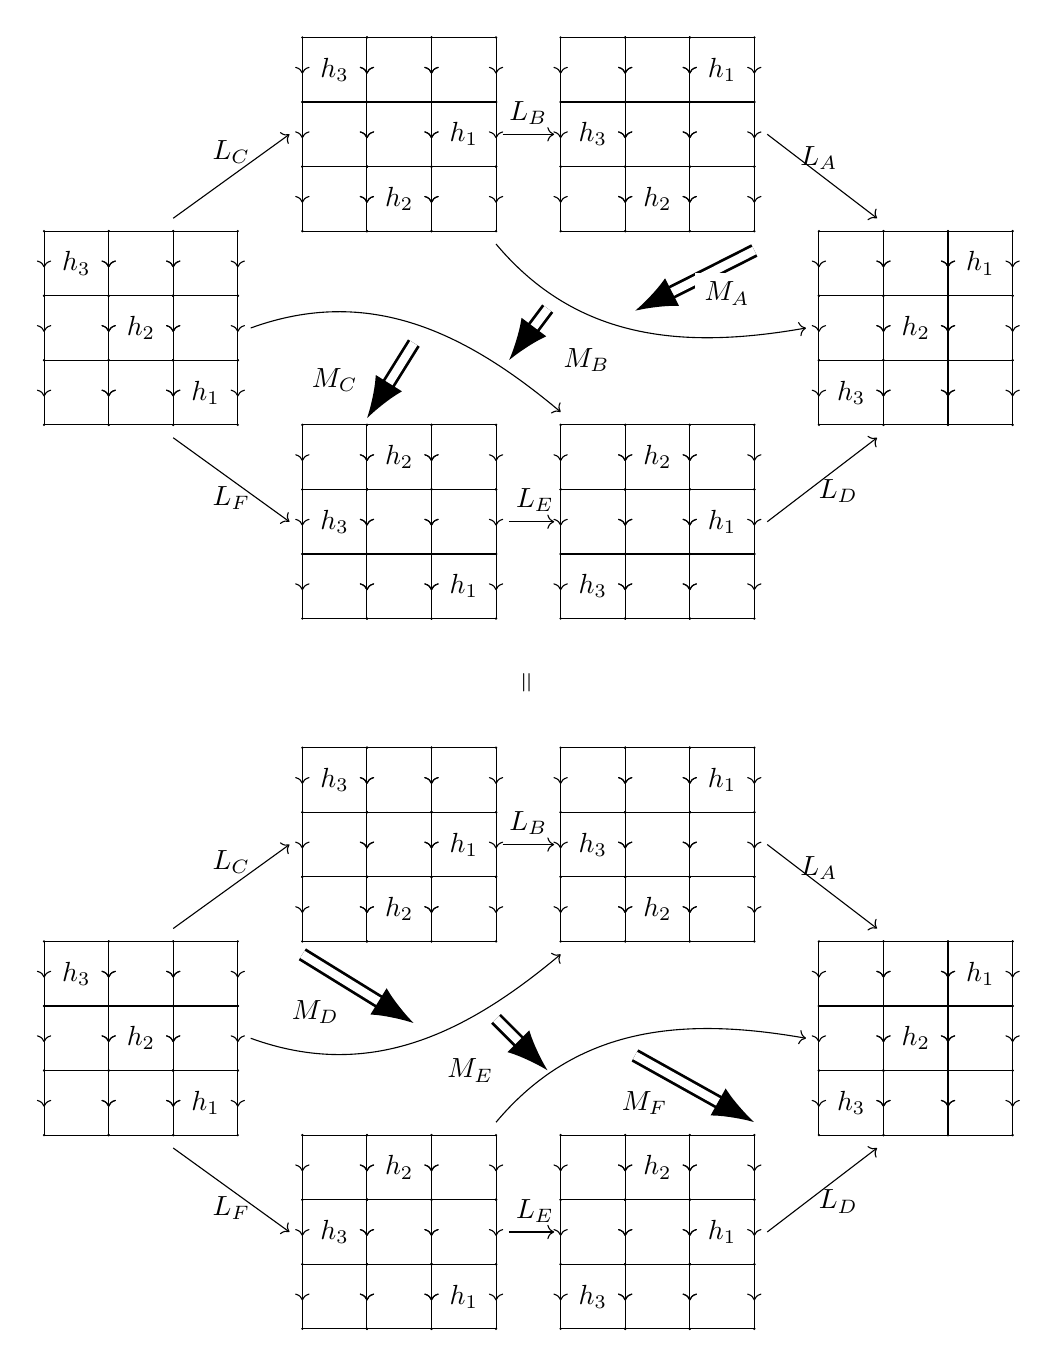
\begin{tikzpicture}[scale=0.82]
  \begin{scope}[xshift=0.0cm]
  \draw[->] (2.0,0.2) to (3.8,1.5);
      \node at (2.9,0.9) [above]{$L_C$};
 \draw[->] (2.0,-3.2) to (3.8,-4.5);
      \node at (2.9,-3.8) [below]{$L_F$};      
  	\begin{scope}[xshift=0.0cm]
	      \draw (0,0) to node[sloped] {\tikz{\draw[->](0,0)--(0.1,0);}} (0,-1);
	      \draw (1,0) to node[sloped] {\tikz{\draw[->](0,0)--(0.1,0);}} (1,-1);
	      \draw (0,0) to node[sloped] {\tikz{\draw[-](0,0)--(0.1,0);}} (1,0);
	      \draw (0,-1) to node  {\tikz{\draw[-](0,0)--(0.1,0);}} (1,-1);
	      \node at (1/2,-1/2) {$h_3$};
	      \draw (0,0) to node {\tikz{\draw[-](0,0)--(0.1,0);}}(1,0);
	      \draw (0,-1) to node {\tikz{\draw[-](0,0)--(0.1,0);}} (1,-1);
	      \fill[black] (0,0) circle[radius=0.02];
	      \fill[black] (1,0) circle[radius=0.02];
	      \fill[black] (0,-1) circle[radius=0.02];
	      \fill[black] (1,-1) circle[radius=0.02];
	    \begin{scope}[xshift=1.0cm]
	      \draw (0,0) to node[sloped] {\tikz{\draw[->](0,0)--(0.1,0);}} (0,-1);
	      \draw (1,0) to node[sloped] {\tikz{\draw[->](0,0)--(0.1,0);}} (1,-1);
	      \draw (0,0) to node[sloped] {\tikz{\draw[-](0,0)--(0.1,0);}} (1,0);
	      \draw (0,-1) to node  {\tikz{\draw[-](0,0)--(0.1,0);}} (1,-1);
	      \node at (1/2,-1/2) {$$};
	      \draw (0,0) to node {\tikz{\draw[-](0,0)--(0.1,0);}} (1,0);
	      \draw (0,-1) to node {\tikz{\draw[-](0,0)--(0.1,0);}} (1,-1);
	      \fill[black] (0,0) circle[radius=0.02];
	      \fill[black] (1,0) circle[radius=0.02];
	      \fill[black] (0,-1) circle[radius=0.02];
	      \fill[black] (1,-1) circle[radius=0.02];
	    \end{scope}
	    	 \begin{scope}[xshift=2.0cm]
	      \draw (0,0) to node[sloped] {\tikz{\draw[->](0,0)--(0.1,0);}} (0,-1);
	      \draw (1,0) to node[sloped] {\tikz{\draw[->](0,0)--(0.1,0);}} (1,-1);
	      \draw (0,0) to node[sloped] {\tikz{\draw[-](0,0)--(0.1,0);}} (1,0);
	      \draw (0,-1) to node  {\tikz{\draw[-](0,0)--(0.1,0);}} (1,-1);
	      \node at (1/2,-1/2) {$$};
	      \draw (0,0) to node {\tikz{\draw[-](0,0)--(0.1,0);}} (1,0);
	      \draw (0,-1) to node {\tikz{\draw[-](0,0)--(0.1,0);}} (1,-1);
	      \fill[black] (0,0) circle[radius=0.02];
	      \fill[black] (1,0) circle[radius=0.02];
	      \fill[black] (0,-1) circle[radius=0.02];
	      \fill[black] (1,-1) circle[radius=0.02];
	    \end{scope}
	     \end{scope}
	     %%%%%%%%%%%%%%%%%%%%%
	\begin{scope}[yshift=-1.0cm]
  	\begin{scope}[xshift=0.0cm]
	      \draw (0,0) to node[sloped] {\tikz{\draw[->](0,0)--(0.1,0);}} (0,-1);
	      \draw (1,0) to node[sloped] {\tikz{\draw[->](0,0)--(0.1,0);}} (1,-1);
	      \draw (0,0) to node[sloped] {\tikz{\draw[-](0,0)--(0.1,0);}} (1,0);
	      \draw (0,-1) to node  {\tikz{\draw[-](0,0)--(0.1,0);}} (1,-1);
	      \node at (1/2,-1/2) {$$};
	      \draw (0,0) to node {\tikz{\draw[-](0,0)--(0.1,0);}}(1,0);
	      \draw (0,-1) to node {\tikz{\draw[-](0,0)--(0.1,0);}} (1,-1);
	      \fill[black] (0,0) circle[radius=0.02];
	      \fill[black] (1,0) circle[radius=0.02];
	      \fill[black] (0,-1) circle[radius=0.02];
	      \fill[black] (1,-1) circle[radius=0.02];
	      \end{scope}
	    \begin{scope}[xshift=1.0cm]
	      \draw (0,0) to node[sloped] {\tikz{\draw[->](0,0)--(0.1,0);}} (0,-1);
	      \draw (1,0) to node[sloped] {\tikz{\draw[->](0,0)--(0.1,0);}} (1,-1);
	      \draw (0,0) to node[sloped] {\tikz{\draw[-](0,0)--(0.1,0);}} (1,0);
	      \draw (0,-1) to node  {\tikz{\draw[-](0,0)--(0.1,0);}} (1,-1);
	      \node at (1/2,-1/2) {$h_2$};
	      \draw (0,0) to node {\tikz{\draw[-](0,0)--(0.1,0);}} (1,0);
	      \draw (0,-1) to node {\tikz{\draw[-](0,0)--(0.1,0);}} (1,-1);
	      \fill[black] (0,0) circle[radius=0.02];
	      \fill[black] (1,0) circle[radius=0.02];
	      \fill[black] (0,-1) circle[radius=0.02];
	      \fill[black] (1,-1) circle[radius=0.02];
	    \end{scope}
	    	 \begin{scope}[xshift=2.0cm]
	      \draw (0,0) to node[sloped] {\tikz{\draw[->](0,0)--(0.1,0);}} (0,-1);
	      \draw (1,0) to node[sloped] {\tikz{\draw[->](0,0)--(0.1,0);}} (1,-1);
	      \draw (0,0) to node[sloped] {\tikz{\draw[-](0,0)--(0.1,0);}} (1,0);
	      \draw (0,-1) to node  {\tikz{\draw[-](0,0)--(0.1,0);}} (1,-1);
	      \node at (1/2,-1/2) {$$};
	      \draw (0,0) to node {\tikz{\draw[-](0,0)--(0.1,0);}} (1,0);
	      \draw (0,-1) to node {\tikz{\draw[-](0,0)--(0.1,0);}} (1,-1);
	      \fill[black] (0,0) circle[radius=0.02];
	      \fill[black] (1,0) circle[radius=0.02];
	      \fill[black] (0,-1) circle[radius=0.02];
	      \fill[black] (1,-1) circle[radius=0.02];
	    \end{scope}
	     \end{scope}
	       %%%%%%%%%%%%%%%%%%%%%
	     \begin{scope}[yshift=-2.0cm]
  	\begin{scope}[xshift=0.0cm]
	      \draw (0,0) to node[sloped] {\tikz{\draw[->](0,0)--(0.1,0);}} (0,-1);
	      \draw (1,0) to node[sloped] {\tikz{\draw[->](0,0)--(0.1,0);}} (1,-1);
	      \draw (0,0) to node[sloped] {\tikz{\draw[-](0,0)--(0.1,0);}} (1,0);
	      \draw (0,-1) to node  {\tikz{\draw[-](0,0)--(0.1,0);}} (1,-1);
	      \node at (1/2,-1/2) {$$};
	      \draw (0,0) to node {\tikz{\draw[-](0,0)--(0.1,0);}}(1,0);
	      \draw (0,-1) to node {\tikz{\draw[-](0,0)--(0.1,0);}} (1,-1);
	      \fill[black] (0,0) circle[radius=0.02];
	      \fill[black] (1,0) circle[radius=0.02];
	      \fill[black] (0,-1) circle[radius=0.02];
	      \fill[black] (1,-1) circle[radius=0.02];
	      \end{scope}
	    \begin{scope}[xshift=1.0cm]
	      \draw (0,0) to node[sloped] {\tikz{\draw[->](0,0)--(0.1,0);}} (0,-1);
	      \draw (1,0) to node[sloped] {\tikz{\draw[->](0,0)--(0.1,0);}} (1,-1);
	      \draw (0,0) to node[sloped] {\tikz{\draw[-](0,0)--(0.1,0);}} (1,0);
	      \draw (0,-1) to node  {\tikz{\draw[-](0,0)--(0.1,0);}} (1,-1);
	      \node at (1/2,-1/2) {$$};
	      \draw (0,0) to node {\tikz{\draw[-](0,0)--(0.1,0);}} (1,0);
	      \draw (0,-1) to node {\tikz{\draw[-](0,0)--(0.1,0);}} (1,-1);
	      \fill[black] (0,0) circle[radius=0.02];
	      \fill[black] (1,0) circle[radius=0.02];
	      \fill[black] (0,-1) circle[radius=0.02];
	      \fill[black] (1,-1) circle[radius=0.02];
	    \end{scope}
	    	 \begin{scope}[xshift=2.0cm]
	      \draw (0,0) to node[sloped] {\tikz{\draw[->](0,0)--(0.1,0);}} (0,-1);
	      \draw (1,0) to node[sloped] {\tikz{\draw[->](0,0)--(0.1,0);}} (1,-1);
	      \draw (0,0) to node[sloped] {\tikz{\draw[-](0,0)--(0.1,0);}} (1,0);
	      \draw (0,-1) to node  {\tikz{\draw[-](0,0)--(0.1,0);}} (1,-1);
	      \node at (1/2,-1/2) {$h_1$};
	      \draw (0,0) to node {\tikz{\draw[-](0,0)--(0.1,0);}} (1,0);
	      \draw (0,-1) to node {\tikz{\draw[-](0,0)--(0.1,0);}} (1,-1);
	      \fill[black] (0,0) circle[radius=0.02];
	      \fill[black] (1,0) circle[radius=0.02];
	      \fill[black] (0,-1) circle[radius=0.02];
	      \fill[black] (1,-1) circle[radius=0.02];
	    \end{scope}
	     \end{scope}
	      \end{scope}
	     %%%%%%%%%%%%%%%%
	     %%%%%%%%%%%%%%%%
	     %%%%%%%%%%%%%%%
	     %%%%%%%%%%%%%%%%
	     \begin{scope}[xshift=4.0cm, yshift=3.0cm]
  \draw[->] (3.1,-1.5) to (3.9,-1.5);
      \node at (3.5,-1.5) [above]{$L_B$};
  	\begin{scope}[xshift=0.0cm]
	      \draw (0,0) to node[sloped] {\tikz{\draw[->](0,0)--(0.1,0);}} (0,-1);
	      \draw (1,0) to node[sloped] {\tikz{\draw[->](0,0)--(0.1,0);}} (1,-1);
	      \draw (0,0) to node[sloped] {\tikz{\draw[-](0,0)--(0.1,0);}} (1,0);
	      \draw (0,-1) to node  {\tikz{\draw[-](0,0)--(0.1,0);}} (1,-1);
	      \node at (1/2,-1/2) {$h_3$};
	      \draw (0,0) to node {\tikz{\draw[-](0,0)--(0.1,0);}}(1,0);
	      \draw (0,-1) to node {\tikz{\draw[-](0,0)--(0.1,0);}} (1,-1);
	      \fill[black] (0,0) circle[radius=0.02];
	      \fill[black] (1,0) circle[radius=0.02];
	      \fill[black] (0,-1) circle[radius=0.02];
	      \fill[black] (1,-1) circle[radius=0.02];
	    \begin{scope}[xshift=1.0cm]
	      \draw (0,0) to node[sloped] {\tikz{\draw[->](0,0)--(0.1,0);}} (0,-1);
	      \draw (1,0) to node[sloped] {\tikz{\draw[->](0,0)--(0.1,0);}} (1,-1);
	      \draw (0,0) to node[sloped] {\tikz{\draw[-](0,0)--(0.1,0);}} (1,0);
	      \draw (0,-1) to node  {\tikz{\draw[-](0,0)--(0.1,0);}} (1,-1);
	      \node at (1/2,-1/2) {$$};
	      \draw (0,0) to node {\tikz{\draw[-](0,0)--(0.1,0);}} (1,0);
	      \draw (0,-1) to node {\tikz{\draw[-](0,0)--(0.1,0);}} (1,-1);
	      \fill[black] (0,0) circle[radius=0.02];
	      \fill[black] (1,0) circle[radius=0.02];
	      \fill[black] (0,-1) circle[radius=0.02];
	      \fill[black] (1,-1) circle[radius=0.02];
	    \end{scope}
	    	 \begin{scope}[xshift=2.0cm]
	      \draw (0,0) to node[sloped] {\tikz{\draw[->](0,0)--(0.1,0);}} (0,-1);
	      \draw (1,0) to node[sloped] {\tikz{\draw[->](0,0)--(0.1,0);}} (1,-1);
	      \draw (0,0) to node[sloped] {\tikz{\draw[-](0,0)--(0.1,0);}} (1,0);
	      \draw (0,-1) to node  {\tikz{\draw[-](0,0)--(0.1,0);}} (1,-1);
	      \node at (1/2,-1/2) {$$};
	      \draw (0,0) to node {\tikz{\draw[-](0,0)--(0.1,0);}} (1,0);
	      \draw (0,-1) to node {\tikz{\draw[-](0,0)--(0.1,0);}} (1,-1);
	      \fill[black] (0,0) circle[radius=0.02];
	      \fill[black] (1,0) circle[radius=0.02];
	      \fill[black] (0,-1) circle[radius=0.02];
	      \fill[black] (1,-1) circle[radius=0.02];
	    \end{scope}
	     \end{scope}
	     %%%%%%%%%%%%%%%%%%%%%
	\begin{scope}[yshift=-1.0cm]
  	\begin{scope}[xshift=0.0cm]
	      \draw (0,0) to node[sloped] {\tikz{\draw[->](0,0)--(0.1,0);}} (0,-1);
	      \draw (1,0) to node[sloped] {\tikz{\draw[->](0,0)--(0.1,0);}} (1,-1);
	      \draw (0,0) to node[sloped] {\tikz{\draw[-](0,0)--(0.1,0);}} (1,0);
	      \draw (0,-1) to node  {\tikz{\draw[-](0,0)--(0.1,0);}} (1,-1);
	      \node at (1/2,-1/2) {$$};
	      \draw (0,0) to node {\tikz{\draw[-](0,0)--(0.1,0);}}(1,0);
	      \draw (0,-1) to node {\tikz{\draw[-](0,0)--(0.1,0);}} (1,-1);
	      \fill[black] (0,0) circle[radius=0.02];
	      \fill[black] (1,0) circle[radius=0.02];
	      \fill[black] (0,-1) circle[radius=0.02];
	      \fill[black] (1,-1) circle[radius=0.02];
	      \end{scope}
	    \begin{scope}[xshift=1.0cm]
	      \draw (0,0) to node[sloped] {\tikz{\draw[->](0,0)--(0.1,0);}} (0,-1);
	      \draw (1,0) to node[sloped] {\tikz{\draw[->](0,0)--(0.1,0);}} (1,-1);
	      \draw (0,0) to node[sloped] {\tikz{\draw[-](0,0)--(0.1,0);}} (1,0);
	      \draw (0,-1) to node  {\tikz{\draw[-](0,0)--(0.1,0);}} (1,-1);
	      \node at (1/2,-1/2) {$$};
	      \draw (0,0) to node {\tikz{\draw[-](0,0)--(0.1,0);}} (1,0);
	      \draw (0,-1) to node {\tikz{\draw[-](0,0)--(0.1,0);}} (1,-1);
	      \fill[black] (0,0) circle[radius=0.02];
	      \fill[black] (1,0) circle[radius=0.02];
	      \fill[black] (0,-1) circle[radius=0.02];
	      \fill[black] (1,-1) circle[radius=0.02];
	    \end{scope}
	    	 \begin{scope}[xshift=2.0cm]
	      \draw (0,0) to node[sloped] {\tikz{\draw[->](0,0)--(0.1,0);}} (0,-1);
	      \draw (1,0) to node[sloped] {\tikz{\draw[->](0,0)--(0.1,0);}} (1,-1);
	      \draw (0,0) to node[sloped] {\tikz{\draw[-](0,0)--(0.1,0);}} (1,0);
	      \draw (0,-1) to node  {\tikz{\draw[-](0,0)--(0.1,0);}} (1,-1);
	      \node at (1/2,-1/2) {$h_1$};
	      \draw (0,0) to node {\tikz{\draw[-](0,0)--(0.1,0);}} (1,0);
	      \draw (0,-1) to node {\tikz{\draw[-](0,0)--(0.1,0);}} (1,-1);
	      \fill[black] (0,0) circle[radius=0.02];
	      \fill[black] (1,0) circle[radius=0.02];
	      \fill[black] (0,-1) circle[radius=0.02];
	      \fill[black] (1,-1) circle[radius=0.02];
	    \end{scope}
	     \end{scope}
	       %%%%%%%%%%%%%%%%%%%%%
	     \begin{scope}[yshift=-2.0cm]
  	\begin{scope}[xshift=0.0cm]
	      \draw (0,0) to node[sloped] {\tikz{\draw[->](0,0)--(0.1,0);}} (0,-1);
	      \draw (1,0) to node[sloped] {\tikz{\draw[->](0,0)--(0.1,0);}} (1,-1);
	      \draw (0,0) to node[sloped] {\tikz{\draw[-](0,0)--(0.1,0);}} (1,0);
	      \draw (0,-1) to node  {\tikz{\draw[-](0,0)--(0.1,0);}} (1,-1);
	      \node at (1/2,-1/2) {$$};
	      \draw (0,0) to node {\tikz{\draw[-](0,0)--(0.1,0);}}(1,0);
	      \draw (0,-1) to node {\tikz{\draw[-](0,0)--(0.1,0);}} (1,-1);
	      \fill[black] (0,0) circle[radius=0.02];
	      \fill[black] (1,0) circle[radius=0.02];
	      \fill[black] (0,-1) circle[radius=0.02];
	      \fill[black] (1,-1) circle[radius=0.02];
	      \end{scope}
	    \begin{scope}[xshift=1.0cm]
	      \draw (0,0) to node[sloped] {\tikz{\draw[->](0,0)--(0.1,0);}} (0,-1);
	      \draw (1,0) to node[sloped] {\tikz{\draw[->](0,0)--(0.1,0);}} (1,-1);
	      \draw (0,0) to node[sloped] {\tikz{\draw[-](0,0)--(0.1,0);}} (1,0);
	      \draw (0,-1) to node  {\tikz{\draw[-](0,0)--(0.1,0);}} (1,-1);
	      \node at (1/2,-1/2) {$h_2$};
	      \draw (0,0) to node {\tikz{\draw[-](0,0)--(0.1,0);}} (1,0);
	      \draw (0,-1) to node {\tikz{\draw[-](0,0)--(0.1,0);}} (1,-1);
	      \fill[black] (0,0) circle[radius=0.02];
	      \fill[black] (1,0) circle[radius=0.02];
	      \fill[black] (0,-1) circle[radius=0.02];
	      \fill[black] (1,-1) circle[radius=0.02];
	    \end{scope}
	    	 \begin{scope}[xshift=2.0cm]
	      \draw (0,0) to node[sloped] {\tikz{\draw[->](0,0)--(0.1,0);}} (0,-1);
	      \draw (1,0) to node[sloped] {\tikz{\draw[->](0,0)--(0.1,0);}} (1,-1);
	      \draw (0,0) to node[sloped] {\tikz{\draw[-](0,0)--(0.1,0);}} (1,0);
	      \draw (0,-1) to node  {\tikz{\draw[-](0,0)--(0.1,0);}} (1,-1);
	      \node at (1/2,-1/2) {$$};
	      \draw (0,0) to node {\tikz{\draw[-](0,0)--(0.1,0);}} (1,0);
	      \draw (0,-1) to node {\tikz{\draw[-](0,0)--(0.1,0);}} (1,-1);
	      \fill[black] (0,0) circle[radius=0.02];
	      \fill[black] (1,0) circle[radius=0.02];
	      \fill[black] (0,-1) circle[radius=0.02];
	      \fill[black] (1,-1) circle[radius=0.02];
	    \end{scope}
	     \end{scope}
	      \end{scope}
	      %%%%%%%%%%%%%%%%
	     %%%%%%%%%%%%%%%%
	     %%%%%%%%%%%%%%%
	     %%%%%%%%%%%%%%%%
	     \begin{scope}[xshift=8.0cm, yshift=3.0cm]
  \draw[->] (3.2,-1.5) to (4.9,-2.8);
      \node at (4.0,-2.2) [above]{$L_A$};
  	\begin{scope}[xshift=0.0cm]
	      \draw (0,0) to node[sloped] {\tikz{\draw[->](0,0)--(0.1,0);}} (0,-1);
	      \draw (1,0) to node[sloped] {\tikz{\draw[->](0,0)--(0.1,0);}} (1,-1);
	      \draw (0,0) to node[sloped] {\tikz{\draw[-](0,0)--(0.1,0);}} (1,0);
	      \draw (0,-1) to node  {\tikz{\draw[-](0,0)--(0.1,0);}} (1,-1);
	      \node at (1/2,-1/2) {$$};
	      \draw (0,0) to node {\tikz{\draw[-](0,0)--(0.1,0);}}(1,0);
	      \draw (0,-1) to node {\tikz{\draw[-](0,0)--(0.1,0);}} (1,-1);
	      \fill[black] (0,0) circle[radius=0.02];
	      \fill[black] (1,0) circle[radius=0.02];
	      \fill[black] (0,-1) circle[radius=0.02];
	      \fill[black] (1,-1) circle[radius=0.02];
	    \begin{scope}[xshift=1.0cm]
	      \draw (0,0) to node[sloped] {\tikz{\draw[->](0,0)--(0.1,0);}} (0,-1);
	      \draw (1,0) to node[sloped] {\tikz{\draw[->](0,0)--(0.1,0);}} (1,-1);
	      \draw (0,0) to node[sloped] {\tikz{\draw[-](0,0)--(0.1,0);}} (1,0);
	      \draw (0,-1) to node  {\tikz{\draw[-](0,0)--(0.1,0);}} (1,-1);
	      \node at (1/2,-1/2) {$$};
	      \draw (0,0) to node {\tikz{\draw[-](0,0)--(0.1,0);}} (1,0);
	      \draw (0,-1) to node {\tikz{\draw[-](0,0)--(0.1,0);}} (1,-1);
	      \fill[black] (0,0) circle[radius=0.02];
	      \fill[black] (1,0) circle[radius=0.02];
	      \fill[black] (0,-1) circle[radius=0.02];
	      \fill[black] (1,-1) circle[radius=0.02];
	    \end{scope}
	    	 \begin{scope}[xshift=2.0cm]
	      \draw (0,0) to node[sloped] {\tikz{\draw[->](0,0)--(0.1,0);}} (0,-1);
	      \draw (1,0) to node[sloped] {\tikz{\draw[->](0,0)--(0.1,0);}} (1,-1);
	      \draw (0,0) to node[sloped] {\tikz{\draw[-](0,0)--(0.1,0);}} (1,0);
	      \draw (0,-1) to node  {\tikz{\draw[-](0,0)--(0.1,0);}} (1,-1);
	      \node at (1/2,-1/2) {$h_1$};
	      \draw (0,0) to node {\tikz{\draw[-](0,0)--(0.1,0);}} (1,0);
	      \draw (0,-1) to node {\tikz{\draw[-](0,0)--(0.1,0);}} (1,-1);
	      \fill[black] (0,0) circle[radius=0.02];
	      \fill[black] (1,0) circle[radius=0.02];
	      \fill[black] (0,-1) circle[radius=0.02];
	      \fill[black] (1,-1) circle[radius=0.02];
	    \end{scope}
	     \end{scope}
	     %%%%%%%%%%%%%%%%%%%%%
	\begin{scope}[yshift=-1.0cm]
  	\begin{scope}[xshift=0.0cm]
	      \draw (0,0) to node[sloped] {\tikz{\draw[->](0,0)--(0.1,0);}} (0,-1);
	      \draw (1,0) to node[sloped] {\tikz{\draw[->](0,0)--(0.1,0);}} (1,-1);
	      \draw (0,0) to node[sloped] {\tikz{\draw[-](0,0)--(0.1,0);}} (1,0);
	      \draw (0,-1) to node  {\tikz{\draw[-](0,0)--(0.1,0);}} (1,-1);
	      \node at (1/2,-1/2) {$h_3$};
	      \draw (0,0) to node {\tikz{\draw[-](0,0)--(0.1,0);}}(1,0);
	      \draw (0,-1) to node {\tikz{\draw[-](0,0)--(0.1,0);}} (1,-1);
	      \fill[black] (0,0) circle[radius=0.02];
	      \fill[black] (1,0) circle[radius=0.02];
	      \fill[black] (0,-1) circle[radius=0.02];
	      \fill[black] (1,-1) circle[radius=0.02];
	      \end{scope}
	    \begin{scope}[xshift=1.0cm]
	      \draw (0,0) to node[sloped] {\tikz{\draw[->](0,0)--(0.1,0);}} (0,-1);
	      \draw (1,0) to node[sloped] {\tikz{\draw[->](0,0)--(0.1,0);}} (1,-1);
	      \draw (0,0) to node[sloped] {\tikz{\draw[-](0,0)--(0.1,0);}} (1,0);
	      \draw (0,-1) to node  {\tikz{\draw[-](0,0)--(0.1,0);}} (1,-1);
	      \node at (1/2,-1/2) {$$};
	      \draw (0,0) to node {\tikz{\draw[-](0,0)--(0.1,0);}} (1,0);
	      \draw (0,-1) to node {\tikz{\draw[-](0,0)--(0.1,0);}} (1,-1);
	      \fill[black] (0,0) circle[radius=0.02];
	      \fill[black] (1,0) circle[radius=0.02];
	      \fill[black] (0,-1) circle[radius=0.02];
	      \fill[black] (1,-1) circle[radius=0.02];
	    \end{scope}
	    	 \begin{scope}[xshift=2.0cm]
	      \draw (0,0) to node[sloped] {\tikz{\draw[->](0,0)--(0.1,0);}} (0,-1);
	      \draw (1,0) to node[sloped] {\tikz{\draw[->](0,0)--(0.1,0);}} (1,-1);
	      \draw (0,0) to node[sloped] {\tikz{\draw[-](0,0)--(0.1,0);}} (1,0);
	      \draw (0,-1) to node  {\tikz{\draw[-](0,0)--(0.1,0);}} (1,-1);
	      \node at (1/2,-1/2) {$$};
	      \draw (0,0) to node {\tikz{\draw[-](0,0)--(0.1,0);}} (1,0);
	      \draw (0,-1) to node {\tikz{\draw[-](0,0)--(0.1,0);}} (1,-1);
	      \fill[black] (0,0) circle[radius=0.02];
	      \fill[black] (1,0) circle[radius=0.02];
	      \fill[black] (0,-1) circle[radius=0.02];
	      \fill[black] (1,-1) circle[radius=0.02];
	    \end{scope}
	     \end{scope}
	       %%%%%%%%%%%%%%%%%%%%%
	     \begin{scope}[yshift=-2.0cm]
  	\begin{scope}[xshift=0.0cm]
	      \draw (0,0) to node[sloped] {\tikz{\draw[->](0,0)--(0.1,0);}} (0,-1);
	      \draw (1,0) to node[sloped] {\tikz{\draw[->](0,0)--(0.1,0);}} (1,-1);
	      \draw (0,0) to node[sloped] {\tikz{\draw[-](0,0)--(0.1,0);}} (1,0);
	      \draw (0,-1) to node  {\tikz{\draw[-](0,0)--(0.1,0);}} (1,-1);
	      \node at (1/2,-1/2) {$$};
	      \draw (0,0) to node {\tikz{\draw[-](0,0)--(0.1,0);}}(1,0);
	      \draw (0,-1) to node {\tikz{\draw[-](0,0)--(0.1,0);}} (1,-1);
	      \fill[black] (0,0) circle[radius=0.02];
	      \fill[black] (1,0) circle[radius=0.02];
	      \fill[black] (0,-1) circle[radius=0.02];
	      \fill[black] (1,-1) circle[radius=0.02];
	      \end{scope}
	    \begin{scope}[xshift=1.0cm]
	      \draw (0,0) to node[sloped] {\tikz{\draw[->](0,0)--(0.1,0);}} (0,-1);
	      \draw (1,0) to node[sloped] {\tikz{\draw[->](0,0)--(0.1,0);}} (1,-1);
	      \draw (0,0) to node[sloped] {\tikz{\draw[-](0,0)--(0.1,0);}} (1,0);
	      \draw (0,-1) to node  {\tikz{\draw[-](0,0)--(0.1,0);}} (1,-1);
	      \node at (1/2,-1/2) {$h_2$};
	      \draw (0,0) to node {\tikz{\draw[-](0,0)--(0.1,0);}} (1,0);
	      \draw (0,-1) to node {\tikz{\draw[-](0,0)--(0.1,0);}} (1,-1);
	      \fill[black] (0,0) circle[radius=0.02];
	      \fill[black] (1,0) circle[radius=0.02];
	      \fill[black] (0,-1) circle[radius=0.02];
	      \fill[black] (1,-1) circle[radius=0.02];
	    \end{scope}
	    	 \begin{scope}[xshift=2.0cm]
	      \draw (0,0) to node[sloped] {\tikz{\draw[->](0,0)--(0.1,0);}} (0,-1);
	      \draw (1,0) to node[sloped] {\tikz{\draw[->](0,0)--(0.1,0);}} (1,-1);
	      \draw (0,0) to node[sloped] {\tikz{\draw[-](0,0)--(0.1,0);}} (1,0);
	      \draw (0,-1) to node  {\tikz{\draw[-](0,0)--(0.1,0);}} (1,-1);
	      \node at (1/2,-1/2) {$$};
	      \draw (0,0) to node {\tikz{\draw[-](0,0)--(0.1,0);}} (1,0);
	      \draw (0,-1) to node {\tikz{\draw[-](0,0)--(0.1,0);}} (1,-1);
	      \fill[black] (0,0) circle[radius=0.02];
	      \fill[black] (1,0) circle[radius=0.02];
	      \fill[black] (0,-1) circle[radius=0.02];
	      \fill[black] (1,-1) circle[radius=0.02];
	    \end{scope}
	     \end{scope}
	      \end{scope}
	      %%%%%%%%%%%%%%%%
	     %%%%%%%%%%%%%%%%
	     %%%%%%%%%%%%%%%
	     %%%%%%%%%%%%%%%%
	     \begin{scope}[xshift=12.0cm, yshift=0.0cm]
  	\begin{scope}[xshift=0.0cm]
	      \draw (0,0) to node[sloped] {\tikz{\draw[->](0,0)--(0.1,0);}} (0,-1);
	      \draw (1,0) to node[sloped] {\tikz{\draw[->](0,0)--(0.1,0);}} (1,-1);
	      \draw (0,0) to node[sloped] {\tikz{\draw[-](0,0)--(0.1,0);}} (1,0);
	      \draw (0,-1) to node  {\tikz{\draw[-](0,0)--(0.1,0);}} (1,-1);
	      \node at (1/2,-1/2) {$$};
	      \draw (0,0) to node {\tikz{\draw[-](0,0)--(0.1,0);}}(1,0);
	      \draw (0,-1) to node {\tikz{\draw[-](0,0)--(0.1,0);}} (1,-1);
	      \fill[black] (0,0) circle[radius=0.02];
	      \fill[black] (1,0) circle[radius=0.02];
	      \fill[black] (0,-1) circle[radius=0.02];
	      \fill[black] (1,-1) circle[radius=0.02];
	    \begin{scope}[xshift=1.0cm]
	      \draw (0,0) to node[sloped] {\tikz{\draw[->](0,0)--(0.1,0);}} (0,-1);
	      \draw (1,0) to node[sloped] {\tikz{\draw[->](0,0)--(0.1,0);}} (1,-1);
	      \draw (0,0) to node[sloped] {\tikz{\draw[-](0,0)--(0.1,0);}} (1,0);
	      \draw (0,-1) to node  {\tikz{\draw[-](0,0)--(0.1,0);}} (1,-1);
	      \node at (1/2,-1/2) {$$};
	      \draw (0,0) to node {\tikz{\draw[-](0,0)--(0.1,0);}} (1,0);
	      \draw (0,-1) to node {\tikz{\draw[-](0,0)--(0.1,0);}} (1,-1);
	      \fill[black] (0,0) circle[radius=0.02];
	      \fill[black] (1,0) circle[radius=0.02];
	      \fill[black] (0,-1) circle[radius=0.02];
	      \fill[black] (1,-1) circle[radius=0.02];
	    \end{scope}
	    	 \begin{scope}[xshift=2.0cm]
	      \draw (0,0) to node[sloped] {\tikz{\draw[->](0,0)--(0.1,0);}} (0,-1);
	      \draw (1,0) to node[sloped] {\tikz{\draw[->](0,0)--(0.1,0);}} (1,-1);
	      \draw (0,0) to node[sloped] {\tikz{\draw[-](0,0)--(0.1,0);}} (1,0);
	      \draw (0,-1) to node  {\tikz{\draw[-](0,0)--(0.1,0);}} (1,-1);
	      \node at (1/2,-1/2) {$h_1$};
	      \draw (0,0) to node {\tikz{\draw[-](0,0)--(0.1,0);}} (1,0);
	      \draw (0,-1) to node {\tikz{\draw[-](0,0)--(0.1,0);}} (1,-1);
	      \fill[black] (0,0) circle[radius=0.02];
	      \fill[black] (1,0) circle[radius=0.02];
	      \fill[black] (0,-1) circle[radius=0.02];
	      \fill[black] (1,-1) circle[radius=0.02];
	    \end{scope}
	     \end{scope}
	     %%%%%%%%%%%%%%%%%%%%%
	\begin{scope}[yshift=-1.0cm]
  	\begin{scope}[xshift=0.0cm]
	      \draw (0,0) to node[sloped] {\tikz{\draw[->](0,0)--(0.1,0);}} (0,-1);
	      \draw (1,0) to node[sloped] {\tikz{\draw[->](0,0)--(0.1,0);}} (1,-1);
	      \draw (0,0) to node[sloped] {\tikz{\draw[-](0,0)--(0.1,0);}} (1,0);
	      \draw (0,-1) to node  {\tikz{\draw[-](0,0)--(0.1,0);}} (1,-1);
	      \node at (1/2,-1/2) {$$};
	      \draw (0,0) to node {\tikz{\draw[-](0,0)--(0.1,0);}}(1,0);
	      \draw (0,-1) to node {\tikz{\draw[-](0,0)--(0.1,0);}} (1,-1);
	      \fill[black] (0,0) circle[radius=0.02];
	      \fill[black] (1,0) circle[radius=0.02];
	      \fill[black] (0,-1) circle[radius=0.02];
	      \fill[black] (1,-1) circle[radius=0.02];
	      \end{scope}
	    \begin{scope}[xshift=1.0cm]
	      \draw (0,0) to node[sloped] {\tikz{\draw[->](0,0)--(0.1,0);}} (0,-1);
	      \draw (1,0) to node[sloped] {\tikz{\draw[->](0,0)--(0.1,0);}} (1,-1);
	      \draw (0,0) to node[sloped] {\tikz{\draw[-](0,0)--(0.1,0);}} (1,0);
	      \draw (0,-1) to node  {\tikz{\draw[-](0,0)--(0.1,0);}} (1,-1);
	      \node at (1/2,-1/2) {$h_2$};
	      \draw (0,0) to node {\tikz{\draw[-](0,0)--(0.1,0);}} (1,0);
	      \draw (0,-1) to node {\tikz{\draw[-](0,0)--(0.1,0);}} (1,-1);
	      \fill[black] (0,0) circle[radius=0.02];
	      \fill[black] (1,0) circle[radius=0.02];
	      \fill[black] (0,-1) circle[radius=0.02];
	      \fill[black] (1,-1) circle[radius=0.02];
	    \end{scope}
	    	 \begin{scope}[xshift=2.0cm]
	      \draw (0,0) to node[sloped] {\tikz{\draw[->](0,0)--(0.1,0);}} (0,-1);
	      \draw (1,0) to node[sloped] {\tikz{\draw[->](0,0)--(0.1,0);}} (1,-1);
	      \draw (0,0) to node[sloped] {\tikz{\draw[-](0,0)--(0.1,0);}} (1,0);
	      \draw (0,-1) to node  {\tikz{\draw[-](0,0)--(0.1,0);}} (1,-1);
	      \node at (1/2,-1/2) {$$};
	      \draw (0,0) to node {\tikz{\draw[-](0,0)--(0.1,0);}} (1,0);
	      \draw (0,-1) to node {\tikz{\draw[-](0,0)--(0.1,0);}} (1,-1);
	      \fill[black] (0,0) circle[radius=0.02];
	      \fill[black] (1,0) circle[radius=0.02];
	      \fill[black] (0,-1) circle[radius=0.02];
	      \fill[black] (1,-1) circle[radius=0.02];
	    \end{scope}
	     \end{scope}
	       %%%%%%%%%%%%%%%%%%%%%
	     \begin{scope}[yshift=-2.0cm]
  	\begin{scope}[xshift=0.0cm]
	      \draw (0,0) to node[sloped] {\tikz{\draw[->](0,0)--(0.1,0);}} (0,-1);
	      \draw (1,0) to node[sloped] {\tikz{\draw[->](0,0)--(0.1,0);}} (1,-1);
	      \draw (0,0) to node[sloped] {\tikz{\draw[-](0,0)--(0.1,0);}} (1,0);
	      \draw (0,-1) to node  {\tikz{\draw[-](0,0)--(0.1,0);}} (1,-1);
	      \node at (1/2,-1/2) {$h_3$};
	      \draw (0,0) to node {\tikz{\draw[-](0,0)--(0.1,0);}}(1,0);
	      \draw (0,-1) to node {\tikz{\draw[-](0,0)--(0.1,0);}} (1,-1);
	      \fill[black] (0,0) circle[radius=0.02];
	      \fill[black] (1,0) circle[radius=0.02];
	      \fill[black] (0,-1) circle[radius=0.02];
	      \fill[black] (1,-1) circle[radius=0.02];
	      \end{scope}
	    \begin{scope}[xshift=1.0cm]
	      \draw (0,0) to node[sloped] {\tikz{\draw[->](0,0)--(0.1,0);}} (0,-1);
	      \draw (1,0) to node[sloped] {\tikz{\draw[->](0,0)--(0.1,0);}} (1,-1);
	      \draw (0,0) to node[sloped] {\tikz{\draw[-](0,0)--(0.1,0);}} (1,0);
	      \draw (0,-1) to node  {\tikz{\draw[-](0,0)--(0.1,0);}} (1,-1);
	      \node at (1/2,-1/2) {$$};
	      \draw (0,0) to node {\tikz{\draw[-](0,0)--(0.1,0);}} (1,0);
	      \draw (0,-1) to node {\tikz{\draw[-](0,0)--(0.1,0);}} (1,-1);
	      \fill[black] (0,0) circle[radius=0.02];
	      \fill[black] (1,0) circle[radius=0.02];
	      \fill[black] (0,-1) circle[radius=0.02];
	      \fill[black] (1,-1) circle[radius=0.02];
	    \end{scope}
	    	 \begin{scope}[xshift=2.0cm]
	      \draw (0,0) to node[sloped] {\tikz{\draw[->](0,0)--(0.1,0);}} (0,-1);
	      \draw (1,0) to node[sloped] {\tikz{\draw[->](0,0)--(0.1,0);}} (1,-1);
	      \draw (0,0) to node[sloped] {\tikz{\draw[-](0,0)--(0.1,0);}} (1,0);
	      \draw (0,-1) to node  {\tikz{\draw[-](0,0)--(0.1,0);}} (1,-1);
	      \node at (1/2,-1/2) {$$};
	      \draw (0,0) to node {\tikz{\draw[-](0,0)--(0.1,0);}} (1,0);
	      \draw (0,-1) to node {\tikz{\draw[-](0,0)--(0.1,0);}} (1,-1);
	      \fill[black] (0,0) circle[radius=0.02];
	      \fill[black] (1,0) circle[radius=0.02];
	      \fill[black] (0,-1) circle[radius=0.02];
	      \fill[black] (1,-1) circle[radius=0.02];
	    \end{scope}
	     \end{scope}
	      \end{scope}
	      %%%%%%%%%%%%%%%%
	     %%%%%%%%%%%%%%%%
	     %%%%%%%%%%%%%%%
	     %%%%%%%%%%%%%%%%
	     \begin{scope}[xshift=4.0cm, yshift=-3.0cm]
  \draw[->] (3.2,-1.5) to (3.9,-1.5);
      \node at (3.6,-1.5) [above]{$L_E$};
  	\begin{scope}[xshift=0.0cm]
	      \draw (0,0) to node[sloped] {\tikz{\draw[->](0,0)--(0.1,0);}} (0,-1);
	      \draw (1,0) to node[sloped] {\tikz{\draw[->](0,0)--(0.1,0);}} (1,-1);
	      \draw (0,0) to node[sloped] {\tikz{\draw[-](0,0)--(0.1,0);}} (1,0);
	      \draw (0,-1) to node  {\tikz{\draw[-](0,0)--(0.1,0);}} (1,-1);
	      \node at (1/2,-1/2) {$$};
	      \draw (0,0) to node {\tikz{\draw[-](0,0)--(0.1,0);}}(1,0);
	      \draw (0,-1) to node {\tikz{\draw[-](0,0)--(0.1,0);}} (1,-1);
	      \fill[black] (0,0) circle[radius=0.02];
	      \fill[black] (1,0) circle[radius=0.02];
	      \fill[black] (0,-1) circle[radius=0.02];
	      \fill[black] (1,-1) circle[radius=0.02];
	    \begin{scope}[xshift=1.0cm]
	      \draw (0,0) to node[sloped] {\tikz{\draw[->](0,0)--(0.1,0);}} (0,-1);
	      \draw (1,0) to node[sloped] {\tikz{\draw[->](0,0)--(0.1,0);}} (1,-1);
	      \draw (0,0) to node[sloped] {\tikz{\draw[-](0,0)--(0.1,0);}} (1,0);
	      \draw (0,-1) to node  {\tikz{\draw[-](0,0)--(0.1,0);}} (1,-1);
	      \node at (1/2,-1/2) {$h_2$};
	      \draw (0,0) to node {\tikz{\draw[-](0,0)--(0.1,0);}} (1,0);
	      \draw (0,-1) to node {\tikz{\draw[-](0,0)--(0.1,0);}} (1,-1);
	      \fill[black] (0,0) circle[radius=0.02];
	      \fill[black] (1,0) circle[radius=0.02];
	      \fill[black] (0,-1) circle[radius=0.02];
	      \fill[black] (1,-1) circle[radius=0.02];
	    \end{scope}
	    	 \begin{scope}[xshift=2.0cm]
	      \draw (0,0) to node[sloped] {\tikz{\draw[->](0,0)--(0.1,0);}} (0,-1);
	      \draw (1,0) to node[sloped] {\tikz{\draw[->](0,0)--(0.1,0);}} (1,-1);
	      \draw (0,0) to node[sloped] {\tikz{\draw[-](0,0)--(0.1,0);}} (1,0);
	      \draw (0,-1) to node  {\tikz{\draw[-](0,0)--(0.1,0);}} (1,-1);
	      \node at (1/2,-1/2) {$$};
	      \draw (0,0) to node {\tikz{\draw[-](0,0)--(0.1,0);}} (1,0);
	      \draw (0,-1) to node {\tikz{\draw[-](0,0)--(0.1,0);}} (1,-1);
	      \fill[black] (0,0) circle[radius=0.02];
	      \fill[black] (1,0) circle[radius=0.02];
	      \fill[black] (0,-1) circle[radius=0.02];
	      \fill[black] (1,-1) circle[radius=0.02];
	    \end{scope}
	     \end{scope}
	     %%%%%%%%%%%%%%%%%%%%%
	\begin{scope}[yshift=-1.0cm]
  	\begin{scope}[xshift=0.0cm]
	      \draw (0,0) to node[sloped] {\tikz{\draw[->](0,0)--(0.1,0);}} (0,-1);
	      \draw (1,0) to node[sloped] {\tikz{\draw[->](0,0)--(0.1,0);}} (1,-1);
	      \draw (0,0) to node[sloped] {\tikz{\draw[-](0,0)--(0.1,0);}} (1,0);
	      \draw (0,-1) to node  {\tikz{\draw[-](0,0)--(0.1,0);}} (1,-1);
	      \node at (1/2,-1/2) {$h_3$};
	      \draw (0,0) to node {\tikz{\draw[-](0,0)--(0.1,0);}}(1,0);
	      \draw (0,-1) to node {\tikz{\draw[-](0,0)--(0.1,0);}} (1,-1);
	      \fill[black] (0,0) circle[radius=0.02];
	      \fill[black] (1,0) circle[radius=0.02];
	      \fill[black] (0,-1) circle[radius=0.02];
	      \fill[black] (1,-1) circle[radius=0.02];
	      \end{scope}
	    \begin{scope}[xshift=1.0cm]
	      \draw (0,0) to node[sloped] {\tikz{\draw[->](0,0)--(0.1,0);}} (0,-1);
	      \draw (1,0) to node[sloped] {\tikz{\draw[->](0,0)--(0.1,0);}} (1,-1);
	      \draw (0,0) to node[sloped] {\tikz{\draw[-](0,0)--(0.1,0);}} (1,0);
	      \draw (0,-1) to node  {\tikz{\draw[-](0,0)--(0.1,0);}} (1,-1);
	      \node at (1/2,-1/2) {$$};
	      \draw (0,0) to node {\tikz{\draw[-](0,0)--(0.1,0);}} (1,0);
	      \draw (0,-1) to node {\tikz{\draw[-](0,0)--(0.1,0);}} (1,-1);
	      \fill[black] (0,0) circle[radius=0.02];
	      \fill[black] (1,0) circle[radius=0.02];
	      \fill[black] (0,-1) circle[radius=0.02];
	      \fill[black] (1,-1) circle[radius=0.02];
	    \end{scope}
	    	 \begin{scope}[xshift=2.0cm]
	      \draw (0,0) to node[sloped] {\tikz{\draw[->](0,0)--(0.1,0);}} (0,-1);
	      \draw (1,0) to node[sloped] {\tikz{\draw[->](0,0)--(0.1,0);}} (1,-1);
	      \draw (0,0) to node[sloped] {\tikz{\draw[-](0,0)--(0.1,0);}} (1,0);
	      \draw (0,-1) to node  {\tikz{\draw[-](0,0)--(0.1,0);}} (1,-1);
	      \node at (1/2,-1/2) {$$};
	      \draw (0,0) to node {\tikz{\draw[-](0,0)--(0.1,0);}} (1,0);
	      \draw (0,-1) to node {\tikz{\draw[-](0,0)--(0.1,0);}} (1,-1);
	      \fill[black] (0,0) circle[radius=0.02];
	      \fill[black] (1,0) circle[radius=0.02];
	      \fill[black] (0,-1) circle[radius=0.02];
	      \fill[black] (1,-1) circle[radius=0.02];
	    \end{scope}
	     \end{scope}
	       %%%%%%%%%%%%%%%%%%%%%
	     \begin{scope}[yshift=-2.0cm]
  	\begin{scope}[xshift=0.0cm]
	      \draw (0,0) to node[sloped] {\tikz{\draw[->](0,0)--(0.1,0);}} (0,-1);
	      \draw (1,0) to node[sloped] {\tikz{\draw[->](0,0)--(0.1,0);}} (1,-1);
	      \draw (0,0) to node[sloped] {\tikz{\draw[-](0,0)--(0.1,0);}} (1,0);
	      \draw (0,-1) to node  {\tikz{\draw[-](0,0)--(0.1,0);}} (1,-1);
	      \node at (1/2,-1/2) {$$};
	      \draw (0,0) to node {\tikz{\draw[-](0,0)--(0.1,0);}}(1,0);
	      \draw (0,-1) to node {\tikz{\draw[-](0,0)--(0.1,0);}} (1,-1);
	      \fill[black] (0,0) circle[radius=0.02];
	      \fill[black] (1,0) circle[radius=0.02];
	      \fill[black] (0,-1) circle[radius=0.02];
	      \fill[black] (1,-1) circle[radius=0.02];
	      \end{scope}
	    \begin{scope}[xshift=1.0cm]
	      \draw (0,0) to node[sloped] {\tikz{\draw[->](0,0)--(0.1,0);}} (0,-1);
	      \draw (1,0) to node[sloped] {\tikz{\draw[->](0,0)--(0.1,0);}} (1,-1);
	      \draw (0,0) to node[sloped] {\tikz{\draw[-](0,0)--(0.1,0);}} (1,0);
	      \draw (0,-1) to node  {\tikz{\draw[-](0,0)--(0.1,0);}} (1,-1);
	      \node at (1/2,-1/2) {$$};
	      \draw (0,0) to node {\tikz{\draw[-](0,0)--(0.1,0);}} (1,0);
	      \draw (0,-1) to node {\tikz{\draw[-](0,0)--(0.1,0);}} (1,-1);
	      \fill[black] (0,0) circle[radius=0.02];
	      \fill[black] (1,0) circle[radius=0.02];
	      \fill[black] (0,-1) circle[radius=0.02];
	      \fill[black] (1,-1) circle[radius=0.02];
	    \end{scope}
	    	 \begin{scope}[xshift=2.0cm]
	      \draw (0,0) to node[sloped] {\tikz{\draw[->](0,0)--(0.1,0);}} (0,-1);
	      \draw (1,0) to node[sloped] {\tikz{\draw[->](0,0)--(0.1,0);}} (1,-1);
	      \draw (0,0) to node[sloped] {\tikz{\draw[-](0,0)--(0.1,0);}} (1,0);
	      \draw (0,-1) to node  {\tikz{\draw[-](0,0)--(0.1,0);}} (1,-1);
	      \node at (1/2,-1/2) {$h_1$};
	      \draw (0,0) to node {\tikz{\draw[-](0,0)--(0.1,0);}} (1,0);
	      \draw (0,-1) to node {\tikz{\draw[-](0,0)--(0.1,0);}} (1,-1);
	      \fill[black] (0,0) circle[radius=0.02];
	      \fill[black] (1,0) circle[radius=0.02];
	      \fill[black] (0,-1) circle[radius=0.02];
	      \fill[black] (1,-1) circle[radius=0.02];
	    \end{scope}
	     \end{scope}
	      \end{scope}
	       %%%%%%%%%%%%%%%%
	     %%%%%%%%%%%%%%%%
	     %%%%%%%%%%%%%%%
	     %%%%%%%%%%%%%%%%
	     \begin{scope}[xshift=8.0cm, yshift=-3.0cm]
  \draw[->] (3.2,-1.5) to (4.9,-0.2);
      \node at (4.3,-0.7) [below]{$L_D$};
  	\begin{scope}[xshift=0.0cm]
	      \draw (0,0) to node[sloped] {\tikz{\draw[->](0,0)--(0.1,0);}} (0,-1);
	      \draw (1,0) to node[sloped] {\tikz{\draw[->](0,0)--(0.1,0);}} (1,-1);
	      \draw (0,0) to node[sloped] {\tikz{\draw[-](0,0)--(0.1,0);}} (1,0);
	      \draw (0,-1) to node  {\tikz{\draw[-](0,0)--(0.1,0);}} (1,-1);
	      \node at (1/2,-1/2) {$$};
	      \draw (0,0) to node {\tikz{\draw[-](0,0)--(0.1,0);}}(1,0);
	      \draw (0,-1) to node {\tikz{\draw[-](0,0)--(0.1,0);}} (1,-1);
	      \fill[black] (0,0) circle[radius=0.02];
	      \fill[black] (1,0) circle[radius=0.02];
	      \fill[black] (0,-1) circle[radius=0.02];
	      \fill[black] (1,-1) circle[radius=0.02];
	    \begin{scope}[xshift=1.0cm]
	      \draw (0,0) to node[sloped] {\tikz{\draw[->](0,0)--(0.1,0);}} (0,-1);
	      \draw (1,0) to node[sloped] {\tikz{\draw[->](0,0)--(0.1,0);}} (1,-1);
	      \draw (0,0) to node[sloped] {\tikz{\draw[-](0,0)--(0.1,0);}} (1,0);
	      \draw (0,-1) to node  {\tikz{\draw[-](0,0)--(0.1,0);}} (1,-1);
	      \node at (1/2,-1/2) {$h_2$};
	      \draw (0,0) to node {\tikz{\draw[-](0,0)--(0.1,0);}} (1,0);
	      \draw (0,-1) to node {\tikz{\draw[-](0,0)--(0.1,0);}} (1,-1);
	      \fill[black] (0,0) circle[radius=0.02];
	      \fill[black] (1,0) circle[radius=0.02];
	      \fill[black] (0,-1) circle[radius=0.02];
	      \fill[black] (1,-1) circle[radius=0.02];
	    \end{scope}
	    	 \begin{scope}[xshift=2.0cm]
	      \draw (0,0) to node[sloped] {\tikz{\draw[->](0,0)--(0.1,0);}} (0,-1);
	      \draw (1,0) to node[sloped] {\tikz{\draw[->](0,0)--(0.1,0);}} (1,-1);
	      \draw (0,0) to node[sloped] {\tikz{\draw[-](0,0)--(0.1,0);}} (1,0);
	      \draw (0,-1) to node  {\tikz{\draw[-](0,0)--(0.1,0);}} (1,-1);
	      \node at (1/2,-1/2) {$$};
	      \draw (0,0) to node {\tikz{\draw[-](0,0)--(0.1,0);}} (1,0);
	      \draw (0,-1) to node {\tikz{\draw[-](0,0)--(0.1,0);}} (1,-1);
	      \fill[black] (0,0) circle[radius=0.02];
	      \fill[black] (1,0) circle[radius=0.02];
	      \fill[black] (0,-1) circle[radius=0.02];
	      \fill[black] (1,-1) circle[radius=0.02];
	    \end{scope}
	     \end{scope}
	     %%%%%%%%%%%%%%%%%%%%%
	\begin{scope}[yshift=-1.0cm]
  	\begin{scope}[xshift=0.0cm]
	      \draw (0,0) to node[sloped] {\tikz{\draw[->](0,0)--(0.1,0);}} (0,-1);
	      \draw (1,0) to node[sloped] {\tikz{\draw[->](0,0)--(0.1,0);}} (1,-1);
	      \draw (0,0) to node[sloped] {\tikz{\draw[-](0,0)--(0.1,0);}} (1,0);
	      \draw (0,-1) to node  {\tikz{\draw[-](0,0)--(0.1,0);}} (1,-1);
	      \node at (1/2,-1/2) {$$};
	      \draw (0,0) to node {\tikz{\draw[-](0,0)--(0.1,0);}}(1,0);
	      \draw (0,-1) to node {\tikz{\draw[-](0,0)--(0.1,0);}} (1,-1);
	      \fill[black] (0,0) circle[radius=0.02];
	      \fill[black] (1,0) circle[radius=0.02];
	      \fill[black] (0,-1) circle[radius=0.02];
	      \fill[black] (1,-1) circle[radius=0.02];
	      \end{scope}
	    \begin{scope}[xshift=1.0cm]
	      \draw (0,0) to node[sloped] {\tikz{\draw[->](0,0)--(0.1,0);}} (0,-1);
	      \draw (1,0) to node[sloped] {\tikz{\draw[->](0,0)--(0.1,0);}} (1,-1);
	      \draw (0,0) to node[sloped] {\tikz{\draw[-](0,0)--(0.1,0);}} (1,0);
	      \draw (0,-1) to node  {\tikz{\draw[-](0,0)--(0.1,0);}} (1,-1);
	      \node at (1/2,-1/2) {$$};
	      \draw (0,0) to node {\tikz{\draw[-](0,0)--(0.1,0);}} (1,0);
	      \draw (0,-1) to node {\tikz{\draw[-](0,0)--(0.1,0);}} (1,-1);
	      \fill[black] (0,0) circle[radius=0.02];
	      \fill[black] (1,0) circle[radius=0.02];
	      \fill[black] (0,-1) circle[radius=0.02];
	      \fill[black] (1,-1) circle[radius=0.02];
	    \end{scope}
	    	 \begin{scope}[xshift=2.0cm]
	      \draw (0,0) to node[sloped] {\tikz{\draw[->](0,0)--(0.1,0);}} (0,-1);
	      \draw (1,0) to node[sloped] {\tikz{\draw[->](0,0)--(0.1,0);}} (1,-1);
	      \draw (0,0) to node[sloped] {\tikz{\draw[-](0,0)--(0.1,0);}} (1,0);
	      \draw (0,-1) to node  {\tikz{\draw[-](0,0)--(0.1,0);}} (1,-1);
	      \node at (1/2,-1/2) {$h_1$};
	      \draw (0,0) to node {\tikz{\draw[-](0,0)--(0.1,0);}} (1,0);
	      \draw (0,-1) to node {\tikz{\draw[-](0,0)--(0.1,0);}} (1,-1);
	      \fill[black] (0,0) circle[radius=0.02];
	      \fill[black] (1,0) circle[radius=0.02];
	      \fill[black] (0,-1) circle[radius=0.02];
	      \fill[black] (1,-1) circle[radius=0.02];
	    \end{scope}
	     \end{scope}
	       %%%%%%%%%%%%%%%%%%%%%
	     \begin{scope}[yshift=-2.0cm]
  	\begin{scope}[xshift=0.0cm]
	      \draw (0,0) to node[sloped] {\tikz{\draw[->](0,0)--(0.1,0);}} (0,-1);
	      \draw (1,0) to node[sloped] {\tikz{\draw[->](0,0)--(0.1,0);}} (1,-1);
	      \draw (0,0) to node[sloped] {\tikz{\draw[-](0,0)--(0.1,0);}} (1,0);
	      \draw (0,-1) to node  {\tikz{\draw[-](0,0)--(0.1,0);}} (1,-1);
	      \node at (1/2,-1/2) {$h_3$};
	      \draw (0,0) to node {\tikz{\draw[-](0,0)--(0.1,0);}}(1,0);
	      \draw (0,-1) to node {\tikz{\draw[-](0,0)--(0.1,0);}} (1,-1);
	      \fill[black] (0,0) circle[radius=0.02];
	      \fill[black] (1,0) circle[radius=0.02];
	      \fill[black] (0,-1) circle[radius=0.02];
	      \fill[black] (1,-1) circle[radius=0.02];
	      \end{scope}
	    \begin{scope}[xshift=1.0cm]
	      \draw (0,0) to node[sloped] {\tikz{\draw[->](0,0)--(0.1,0);}} (0,-1);
	      \draw (1,0) to node[sloped] {\tikz{\draw[->](0,0)--(0.1,0);}} (1,-1);
	      \draw (0,0) to node[sloped] {\tikz{\draw[-](0,0)--(0.1,0);}} (1,0);
	      \draw (0,-1) to node  {\tikz{\draw[-](0,0)--(0.1,0);}} (1,-1);
	      \node at (1/2,-1/2) {$$};
	      \draw (0,0) to node {\tikz{\draw[-](0,0)--(0.1,0);}} (1,0);
	      \draw (0,-1) to node {\tikz{\draw[-](0,0)--(0.1,0);}} (1,-1);
	      \fill[black] (0,0) circle[radius=0.02];
	      \fill[black] (1,0) circle[radius=0.02];
	      \fill[black] (0,-1) circle[radius=0.02];
	      \fill[black] (1,-1) circle[radius=0.02];
	    \end{scope}
	    	 \begin{scope}[xshift=2.0cm]
	      \draw (0,0) to node[sloped] {\tikz{\draw[->](0,0)--(0.1,0);}} (0,-1);
	      \draw (1,0) to node[sloped] {\tikz{\draw[->](0,0)--(0.1,0);}} (1,-1);
	      \draw (0,0) to node[sloped] {\tikz{\draw[-](0,0)--(0.1,0);}} (1,0);
	      \draw (0,-1) to node  {\tikz{\draw[-](0,0)--(0.1,0);}} (1,-1);
	      \node at (1/2,-1/2) {$$};
	      \draw (0,0) to node {\tikz{\draw[-](0,0)--(0.1,0);}} (1,0);
	      \draw (0,-1) to node {\tikz{\draw[-](0,0)--(0.1,0);}} (1,-1);
	      \fill[black] (0,0) circle[radius=0.02];
	      \fill[black] (1,0) circle[radius=0.02];
	      \fill[black] (0,-1) circle[radius=0.02];
	      \fill[black] (1,-1) circle[radius=0.02];
	    \end{scope}
	     \end{scope}
	      \end{scope}
	    \draw[->] (7.0,-0.2) to [out=-50,in=-170] node[midway] (M1) {} (11.8,-1.5)   ;
	      \node[above] at (M1) {$$};
  		\draw [line width=1pt, double distance=3pt, arrows = {-Latex[length=0pt 3 0]}]
        (11.0, -0.3) -- ($(M1) - (0, -0.3)$);
      \node at ($($(11.0, -0.3)!0.5!($(M1) - (0, 0.1)$)$)+(0.5,0.0)$)  [fill=white]{$M_A$};
      
       \draw[->] (3.2,-1.5) to [out=20,in=140] node[midway] (M2) {} (8.0,-2.8)   ;
	      \node[above] at (M2) {$$};
  		\draw [line width=1pt, double distance=3pt, arrows = {-Latex[length=0pt 3 0]}]
        (7.8,-1.2) -- (7.2,-2.0);
      \node at (8.4, -2.0)  []{$M_B$};
      
      \draw [line width=1pt, double distance=3pt, arrows = {-Latex[length=0pt 3 0]}]
        ($(M2) - (0, 0.3)$) -- (5.0, -2.9);
        \node at (4.5, -2.3)  []{$M_C$};
        
        
%%%%%%%%%%%%%%%%%%%%%%%%%%%%%%%%%%%%下にシフトしたやつ%%%%%%%%%%%%%%%%%%%%%%%%%%%%%%%%%%%%%%%%%%%%%%%%%%%%%%%%%%%%%%%%%%%%%%%%%%%%%%%%%%%%%%%%%%%%%%%%%%%%%%%%

\begin{scope}[yshift=-11.0cm]

\begin{scope}[xshift=0.0cm]
  \draw[->] (2.0,0.2) to (3.8,1.5);
      \node at (2.9,0.9) [above]{$L_C$};
 \draw[->] (2.0,-3.2) to (3.8,-4.5);
      \node at (2.9,-3.8) [below]{$L_F$};      
  	\begin{scope}[xshift=0.0cm]
	      \draw (0,0) to node[sloped] {\tikz{\draw[->](0,0)--(0.1,0);}} (0,-1);
	      \draw (1,0) to node[sloped] {\tikz{\draw[->](0,0)--(0.1,0);}} (1,-1);
	      \draw (0,0) to node[sloped] {\tikz{\draw[-](0,0)--(0.1,0);}} (1,0);
	      \draw (0,-1) to node  {\tikz{\draw[-](0,0)--(0.1,0);}} (1,-1);
	      \node at (1/2,-1/2) {$h_3$};
	      \draw (0,0) to node {\tikz{\draw[-](0,0)--(0.1,0);}}(1,0);
	      \draw (0,-1) to node {\tikz{\draw[-](0,0)--(0.1,0);}} (1,-1);
	      \fill[black] (0,0) circle[radius=0.02];
	      \fill[black] (1,0) circle[radius=0.02];
	      \fill[black] (0,-1) circle[radius=0.02];
	      \fill[black] (1,-1) circle[radius=0.02];
	    \begin{scope}[xshift=1.0cm]
	      \draw (0,0) to node[sloped] {\tikz{\draw[->](0,0)--(0.1,0);}} (0,-1);
	      \draw (1,0) to node[sloped] {\tikz{\draw[->](0,0)--(0.1,0);}} (1,-1);
	      \draw (0,0) to node[sloped] {\tikz{\draw[-](0,0)--(0.1,0);}} (1,0);
	      \draw (0,-1) to node  {\tikz{\draw[-](0,0)--(0.1,0);}} (1,-1);
	      \node at (1/2,-1/2) {$$};
	      \draw (0,0) to node {\tikz{\draw[-](0,0)--(0.1,0);}} (1,0);
	      \draw (0,-1) to node {\tikz{\draw[-](0,0)--(0.1,0);}} (1,-1);
	      \fill[black] (0,0) circle[radius=0.02];
	      \fill[black] (1,0) circle[radius=0.02];
	      \fill[black] (0,-1) circle[radius=0.02];
	      \fill[black] (1,-1) circle[radius=0.02];
	    \end{scope}
	    	 \begin{scope}[xshift=2.0cm]
	      \draw (0,0) to node[sloped] {\tikz{\draw[->](0,0)--(0.1,0);}} (0,-1);
	      \draw (1,0) to node[sloped] {\tikz{\draw[->](0,0)--(0.1,0);}} (1,-1);
	      \draw (0,0) to node[sloped] {\tikz{\draw[-](0,0)--(0.1,0);}} (1,0);
	      \draw (0,-1) to node  {\tikz{\draw[-](0,0)--(0.1,0);}} (1,-1);
	      \node at (1/2,-1/2) {$$};
	      \draw (0,0) to node {\tikz{\draw[-](0,0)--(0.1,0);}} (1,0);
	      \draw (0,-1) to node {\tikz{\draw[-](0,0)--(0.1,0);}} (1,-1);
	      \fill[black] (0,0) circle[radius=0.02];
	      \fill[black] (1,0) circle[radius=0.02];
	      \fill[black] (0,-1) circle[radius=0.02];
	      \fill[black] (1,-1) circle[radius=0.02];
	    \end{scope}
	     \end{scope}
	     %%%%%%%%%%%%%%%%%%%%%
	\begin{scope}[yshift=-1.0cm]
  	\begin{scope}[xshift=0.0cm]
	      \draw (0,0) to node[sloped] {\tikz{\draw[->](0,0)--(0.1,0);}} (0,-1);
	      \draw (1,0) to node[sloped] {\tikz{\draw[->](0,0)--(0.1,0);}} (1,-1);
	      \draw (0,0) to node[sloped] {\tikz{\draw[-](0,0)--(0.1,0);}} (1,0);
	      \draw (0,-1) to node  {\tikz{\draw[-](0,0)--(0.1,0);}} (1,-1);
	      \node at (1/2,-1/2) {$$};
	      \draw (0,0) to node {\tikz{\draw[-](0,0)--(0.1,0);}}(1,0);
	      \draw (0,-1) to node {\tikz{\draw[-](0,0)--(0.1,0);}} (1,-1);
	      \fill[black] (0,0) circle[radius=0.02];
	      \fill[black] (1,0) circle[radius=0.02];
	      \fill[black] (0,-1) circle[radius=0.02];
	      \fill[black] (1,-1) circle[radius=0.02];
	      \end{scope}
	    \begin{scope}[xshift=1.0cm]
	      \draw (0,0) to node[sloped] {\tikz{\draw[->](0,0)--(0.1,0);}} (0,-1);
	      \draw (1,0) to node[sloped] {\tikz{\draw[->](0,0)--(0.1,0);}} (1,-1);
	      \draw (0,0) to node[sloped] {\tikz{\draw[-](0,0)--(0.1,0);}} (1,0);
	      \draw (0,-1) to node  {\tikz{\draw[-](0,0)--(0.1,0);}} (1,-1);
	      \node at (1/2,-1/2) {$h_2$};
	      \draw (0,0) to node {\tikz{\draw[-](0,0)--(0.1,0);}} (1,0);
	      \draw (0,-1) to node {\tikz{\draw[-](0,0)--(0.1,0);}} (1,-1);
	      \fill[black] (0,0) circle[radius=0.02];
	      \fill[black] (1,0) circle[radius=0.02];
	      \fill[black] (0,-1) circle[radius=0.02];
	      \fill[black] (1,-1) circle[radius=0.02];
	    \end{scope}
	    	 \begin{scope}[xshift=2.0cm]
	      \draw (0,0) to node[sloped] {\tikz{\draw[->](0,0)--(0.1,0);}} (0,-1);
	      \draw (1,0) to node[sloped] {\tikz{\draw[->](0,0)--(0.1,0);}} (1,-1);
	      \draw (0,0) to node[sloped] {\tikz{\draw[-](0,0)--(0.1,0);}} (1,0);
	      \draw (0,-1) to node  {\tikz{\draw[-](0,0)--(0.1,0);}} (1,-1);
	      \node at (1/2,-1/2) {$$};
	      \draw (0,0) to node {\tikz{\draw[-](0,0)--(0.1,0);}} (1,0);
	      \draw (0,-1) to node {\tikz{\draw[-](0,0)--(0.1,0);}} (1,-1);
	      \fill[black] (0,0) circle[radius=0.02];
	      \fill[black] (1,0) circle[radius=0.02];
	      \fill[black] (0,-1) circle[radius=0.02];
	      \fill[black] (1,-1) circle[radius=0.02];
	    \end{scope}
	     \end{scope}
	       %%%%%%%%%%%%%%%%%%%%%
	     \begin{scope}[yshift=-2.0cm]
  	\begin{scope}[xshift=0.0cm]
	      \draw (0,0) to node[sloped] {\tikz{\draw[->](0,0)--(0.1,0);}} (0,-1);
	      \draw (1,0) to node[sloped] {\tikz{\draw[->](0,0)--(0.1,0);}} (1,-1);
	      \draw (0,0) to node[sloped] {\tikz{\draw[-](0,0)--(0.1,0);}} (1,0);
	      \draw (0,-1) to node  {\tikz{\draw[-](0,0)--(0.1,0);}} (1,-1);
	      \node at (1/2,-1/2) {$$};
	      \draw (0,0) to node {\tikz{\draw[-](0,0)--(0.1,0);}}(1,0);
	      \draw (0,-1) to node {\tikz{\draw[-](0,0)--(0.1,0);}} (1,-1);
	      \fill[black] (0,0) circle[radius=0.02];
	      \fill[black] (1,0) circle[radius=0.02];
	      \fill[black] (0,-1) circle[radius=0.02];
	      \fill[black] (1,-1) circle[radius=0.02];
	      \end{scope}
	    \begin{scope}[xshift=1.0cm]
	      \draw (0,0) to node[sloped] {\tikz{\draw[->](0,0)--(0.1,0);}} (0,-1);
	      \draw (1,0) to node[sloped] {\tikz{\draw[->](0,0)--(0.1,0);}} (1,-1);
	      \draw (0,0) to node[sloped] {\tikz{\draw[-](0,0)--(0.1,0);}} (1,0);
	      \draw (0,-1) to node  {\tikz{\draw[-](0,0)--(0.1,0);}} (1,-1);
	      \node at (1/2,-1/2) {$$};
	      \draw (0,0) to node {\tikz{\draw[-](0,0)--(0.1,0);}} (1,0);
	      \draw (0,-1) to node {\tikz{\draw[-](0,0)--(0.1,0);}} (1,-1);
	      \fill[black] (0,0) circle[radius=0.02];
	      \fill[black] (1,0) circle[radius=0.02];
	      \fill[black] (0,-1) circle[radius=0.02];
	      \fill[black] (1,-1) circle[radius=0.02];
	    \end{scope}
	    	 \begin{scope}[xshift=2.0cm]
	      \draw (0,0) to node[sloped] {\tikz{\draw[->](0,0)--(0.1,0);}} (0,-1);
	      \draw (1,0) to node[sloped] {\tikz{\draw[->](0,0)--(0.1,0);}} (1,-1);
	      \draw (0,0) to node[sloped] {\tikz{\draw[-](0,0)--(0.1,0);}} (1,0);
	      \draw (0,-1) to node  {\tikz{\draw[-](0,0)--(0.1,0);}} (1,-1);
	      \node at (1/2,-1/2) {$h_1$};
	      \draw (0,0) to node {\tikz{\draw[-](0,0)--(0.1,0);}} (1,0);
	      \draw (0,-1) to node {\tikz{\draw[-](0,0)--(0.1,0);}} (1,-1);
	      \fill[black] (0,0) circle[radius=0.02];
	      \fill[black] (1,0) circle[radius=0.02];
	      \fill[black] (0,-1) circle[radius=0.02];
	      \fill[black] (1,-1) circle[radius=0.02];
	    \end{scope}
	     \end{scope}
	      \end{scope}
	     %%%%%%%%%%%%%%%%
	     %%%%%%%%%%%%%%%%
	     %%%%%%%%%%%%%%%
	     %%%%%%%%%%%%%%%%
	     \begin{scope}[xshift=4.0cm, yshift=3.0cm]
  \draw[->] (3.1,-1.5) to (3.9,-1.5);
      \node at (3.5,-1.5) [above]{$L_B$};
  	\begin{scope}[xshift=0.0cm]
	      \draw (0,0) to node[sloped] {\tikz{\draw[->](0,0)--(0.1,0);}} (0,-1);
	      \draw (1,0) to node[sloped] {\tikz{\draw[->](0,0)--(0.1,0);}} (1,-1);
	      \draw (0,0) to node[sloped] {\tikz{\draw[-](0,0)--(0.1,0);}} (1,0);
	      \draw (0,-1) to node  {\tikz{\draw[-](0,0)--(0.1,0);}} (1,-1);
	      \node at (1/2,-1/2) {$h_3$};
	      \draw (0,0) to node {\tikz{\draw[-](0,0)--(0.1,0);}}(1,0);
	      \draw (0,-1) to node {\tikz{\draw[-](0,0)--(0.1,0);}} (1,-1);
	      \fill[black] (0,0) circle[radius=0.02];
	      \fill[black] (1,0) circle[radius=0.02];
	      \fill[black] (0,-1) circle[radius=0.02];
	      \fill[black] (1,-1) circle[radius=0.02];
	    \begin{scope}[xshift=1.0cm]
	      \draw (0,0) to node[sloped] {\tikz{\draw[->](0,0)--(0.1,0);}} (0,-1);
	      \draw (1,0) to node[sloped] {\tikz{\draw[->](0,0)--(0.1,0);}} (1,-1);
	      \draw (0,0) to node[sloped] {\tikz{\draw[-](0,0)--(0.1,0);}} (1,0);
	      \draw (0,-1) to node  {\tikz{\draw[-](0,0)--(0.1,0);}} (1,-1);
	      \node at (1/2,-1/2) {$$};
	      \draw (0,0) to node {\tikz{\draw[-](0,0)--(0.1,0);}} (1,0);
	      \draw (0,-1) to node {\tikz{\draw[-](0,0)--(0.1,0);}} (1,-1);
	      \fill[black] (0,0) circle[radius=0.02];
	      \fill[black] (1,0) circle[radius=0.02];
	      \fill[black] (0,-1) circle[radius=0.02];
	      \fill[black] (1,-1) circle[radius=0.02];
	    \end{scope}
	    	 \begin{scope}[xshift=2.0cm]
	      \draw (0,0) to node[sloped] {\tikz{\draw[->](0,0)--(0.1,0);}} (0,-1);
	      \draw (1,0) to node[sloped] {\tikz{\draw[->](0,0)--(0.1,0);}} (1,-1);
	      \draw (0,0) to node[sloped] {\tikz{\draw[-](0,0)--(0.1,0);}} (1,0);
	      \draw (0,-1) to node  {\tikz{\draw[-](0,0)--(0.1,0);}} (1,-1);
	      \node at (1/2,-1/2) {$$};
	      \draw (0,0) to node {\tikz{\draw[-](0,0)--(0.1,0);}} (1,0);
	      \draw (0,-1) to node {\tikz{\draw[-](0,0)--(0.1,0);}} (1,-1);
	      \fill[black] (0,0) circle[radius=0.02];
	      \fill[black] (1,0) circle[radius=0.02];
	      \fill[black] (0,-1) circle[radius=0.02];
	      \fill[black] (1,-1) circle[radius=0.02];
	    \end{scope}
	     \end{scope}
	     %%%%%%%%%%%%%%%%%%%%%
	\begin{scope}[yshift=-1.0cm]
  	\begin{scope}[xshift=0.0cm]
	      \draw (0,0) to node[sloped] {\tikz{\draw[->](0,0)--(0.1,0);}} (0,-1);
	      \draw (1,0) to node[sloped] {\tikz{\draw[->](0,0)--(0.1,0);}} (1,-1);
	      \draw (0,0) to node[sloped] {\tikz{\draw[-](0,0)--(0.1,0);}} (1,0);
	      \draw (0,-1) to node  {\tikz{\draw[-](0,0)--(0.1,0);}} (1,-1);
	      \node at (1/2,-1/2) {$$};
	      \draw (0,0) to node {\tikz{\draw[-](0,0)--(0.1,0);}}(1,0);
	      \draw (0,-1) to node {\tikz{\draw[-](0,0)--(0.1,0);}} (1,-1);
	      \fill[black] (0,0) circle[radius=0.02];
	      \fill[black] (1,0) circle[radius=0.02];
	      \fill[black] (0,-1) circle[radius=0.02];
	      \fill[black] (1,-1) circle[radius=0.02];
	      \end{scope}
	    \begin{scope}[xshift=1.0cm]
	      \draw (0,0) to node[sloped] {\tikz{\draw[->](0,0)--(0.1,0);}} (0,-1);
	      \draw (1,0) to node[sloped] {\tikz{\draw[->](0,0)--(0.1,0);}} (1,-1);
	      \draw (0,0) to node[sloped] {\tikz{\draw[-](0,0)--(0.1,0);}} (1,0);
	      \draw (0,-1) to node  {\tikz{\draw[-](0,0)--(0.1,0);}} (1,-1);
	      \node at (1/2,-1/2) {$$};
	      \draw (0,0) to node {\tikz{\draw[-](0,0)--(0.1,0);}} (1,0);
	      \draw (0,-1) to node {\tikz{\draw[-](0,0)--(0.1,0);}} (1,-1);
	      \fill[black] (0,0) circle[radius=0.02];
	      \fill[black] (1,0) circle[radius=0.02];
	      \fill[black] (0,-1) circle[radius=0.02];
	      \fill[black] (1,-1) circle[radius=0.02];
	    \end{scope}
	    	 \begin{scope}[xshift=2.0cm]
	      \draw (0,0) to node[sloped] {\tikz{\draw[->](0,0)--(0.1,0);}} (0,-1);
	      \draw (1,0) to node[sloped] {\tikz{\draw[->](0,0)--(0.1,0);}} (1,-1);
	      \draw (0,0) to node[sloped] {\tikz{\draw[-](0,0)--(0.1,0);}} (1,0);
	      \draw (0,-1) to node  {\tikz{\draw[-](0,0)--(0.1,0);}} (1,-1);
	      \node at (1/2,-1/2) {$h_1$};
	      \draw (0,0) to node {\tikz{\draw[-](0,0)--(0.1,0);}} (1,0);
	      \draw (0,-1) to node {\tikz{\draw[-](0,0)--(0.1,0);}} (1,-1);
	      \fill[black] (0,0) circle[radius=0.02];
	      \fill[black] (1,0) circle[radius=0.02];
	      \fill[black] (0,-1) circle[radius=0.02];
	      \fill[black] (1,-1) circle[radius=0.02];
	    \end{scope}
	     \end{scope}
	       %%%%%%%%%%%%%%%%%%%%%
	     \begin{scope}[yshift=-2.0cm]
  	\begin{scope}[xshift=0.0cm]
	      \draw (0,0) to node[sloped] {\tikz{\draw[->](0,0)--(0.1,0);}} (0,-1);
	      \draw (1,0) to node[sloped] {\tikz{\draw[->](0,0)--(0.1,0);}} (1,-1);
	      \draw (0,0) to node[sloped] {\tikz{\draw[-](0,0)--(0.1,0);}} (1,0);
	      \draw (0,-1) to node  {\tikz{\draw[-](0,0)--(0.1,0);}} (1,-1);
	      \node at (1/2,-1/2) {$$};
	      \draw (0,0) to node {\tikz{\draw[-](0,0)--(0.1,0);}}(1,0);
	      \draw (0,-1) to node {\tikz{\draw[-](0,0)--(0.1,0);}} (1,-1);
	      \fill[black] (0,0) circle[radius=0.02];
	      \fill[black] (1,0) circle[radius=0.02];
	      \fill[black] (0,-1) circle[radius=0.02];
	      \fill[black] (1,-1) circle[radius=0.02];
	      \end{scope}
	    \begin{scope}[xshift=1.0cm]
	      \draw (0,0) to node[sloped] {\tikz{\draw[->](0,0)--(0.1,0);}} (0,-1);
	      \draw (1,0) to node[sloped] {\tikz{\draw[->](0,0)--(0.1,0);}} (1,-1);
	      \draw (0,0) to node[sloped] {\tikz{\draw[-](0,0)--(0.1,0);}} (1,0);
	      \draw (0,-1) to node  {\tikz{\draw[-](0,0)--(0.1,0);}} (1,-1);
	      \node at (1/2,-1/2) {$h_2$};
	      \draw (0,0) to node {\tikz{\draw[-](0,0)--(0.1,0);}} (1,0);
	      \draw (0,-1) to node {\tikz{\draw[-](0,0)--(0.1,0);}} (1,-1);
	      \fill[black] (0,0) circle[radius=0.02];
	      \fill[black] (1,0) circle[radius=0.02];
	      \fill[black] (0,-1) circle[radius=0.02];
	      \fill[black] (1,-1) circle[radius=0.02];
	    \end{scope}
	    	 \begin{scope}[xshift=2.0cm]
	      \draw (0,0) to node[sloped] {\tikz{\draw[->](0,0)--(0.1,0);}} (0,-1);
	      \draw (1,0) to node[sloped] {\tikz{\draw[->](0,0)--(0.1,0);}} (1,-1);
	      \draw (0,0) to node[sloped] {\tikz{\draw[-](0,0)--(0.1,0);}} (1,0);
	      \draw (0,-1) to node  {\tikz{\draw[-](0,0)--(0.1,0);}} (1,-1);
	      \node at (1/2,-1/2) {$$};
	      \draw (0,0) to node {\tikz{\draw[-](0,0)--(0.1,0);}} (1,0);
	      \draw (0,-1) to node {\tikz{\draw[-](0,0)--(0.1,0);}} (1,-1);
	      \fill[black] (0,0) circle[radius=0.02];
	      \fill[black] (1,0) circle[radius=0.02];
	      \fill[black] (0,-1) circle[radius=0.02];
	      \fill[black] (1,-1) circle[radius=0.02];
	    \end{scope}
	     \end{scope}
	      \end{scope}
	      %%%%%%%%%%%%%%%%
	     %%%%%%%%%%%%%%%%
	     %%%%%%%%%%%%%%%
	     %%%%%%%%%%%%%%%%
	     \begin{scope}[xshift=8.0cm, yshift=3.0cm]
  \draw[->] (3.2,-1.5) to (4.9,-2.8);
      \node at (4.0,-2.2) [above]{$L_A$};
  	\begin{scope}[xshift=0.0cm]
	      \draw (0,0) to node[sloped] {\tikz{\draw[->](0,0)--(0.1,0);}} (0,-1);
	      \draw (1,0) to node[sloped] {\tikz{\draw[->](0,0)--(0.1,0);}} (1,-1);
	      \draw (0,0) to node[sloped] {\tikz{\draw[-](0,0)--(0.1,0);}} (1,0);
	      \draw (0,-1) to node  {\tikz{\draw[-](0,0)--(0.1,0);}} (1,-1);
	      \node at (1/2,-1/2) {$$};
	      \draw (0,0) to node {\tikz{\draw[-](0,0)--(0.1,0);}}(1,0);
	      \draw (0,-1) to node {\tikz{\draw[-](0,0)--(0.1,0);}} (1,-1);
	      \fill[black] (0,0) circle[radius=0.02];
	      \fill[black] (1,0) circle[radius=0.02];
	      \fill[black] (0,-1) circle[radius=0.02];
	      \fill[black] (1,-1) circle[radius=0.02];
	    \begin{scope}[xshift=1.0cm]
	      \draw (0,0) to node[sloped] {\tikz{\draw[->](0,0)--(0.1,0);}} (0,-1);
	      \draw (1,0) to node[sloped] {\tikz{\draw[->](0,0)--(0.1,0);}} (1,-1);
	      \draw (0,0) to node[sloped] {\tikz{\draw[-](0,0)--(0.1,0);}} (1,0);
	      \draw (0,-1) to node  {\tikz{\draw[-](0,0)--(0.1,0);}} (1,-1);
	      \node at (1/2,-1/2) {$$};
	      \draw (0,0) to node {\tikz{\draw[-](0,0)--(0.1,0);}} (1,0);
	      \draw (0,-1) to node {\tikz{\draw[-](0,0)--(0.1,0);}} (1,-1);
	      \fill[black] (0,0) circle[radius=0.02];
	      \fill[black] (1,0) circle[radius=0.02];
	      \fill[black] (0,-1) circle[radius=0.02];
	      \fill[black] (1,-1) circle[radius=0.02];
	    \end{scope}
	    	 \begin{scope}[xshift=2.0cm]
	      \draw (0,0) to node[sloped] {\tikz{\draw[->](0,0)--(0.1,0);}} (0,-1);
	      \draw (1,0) to node[sloped] {\tikz{\draw[->](0,0)--(0.1,0);}} (1,-1);
	      \draw (0,0) to node[sloped] {\tikz{\draw[-](0,0)--(0.1,0);}} (1,0);
	      \draw (0,-1) to node  {\tikz{\draw[-](0,0)--(0.1,0);}} (1,-1);
	      \node at (1/2,-1/2) {$h_1$};
	      \draw (0,0) to node {\tikz{\draw[-](0,0)--(0.1,0);}} (1,0);
	      \draw (0,-1) to node {\tikz{\draw[-](0,0)--(0.1,0);}} (1,-1);
	      \fill[black] (0,0) circle[radius=0.02];
	      \fill[black] (1,0) circle[radius=0.02];
	      \fill[black] (0,-1) circle[radius=0.02];
	      \fill[black] (1,-1) circle[radius=0.02];
	    \end{scope}
	     \end{scope}
	     %%%%%%%%%%%%%%%%%%%%%
	\begin{scope}[yshift=-1.0cm]
  	\begin{scope}[xshift=0.0cm]
	      \draw (0,0) to node[sloped] {\tikz{\draw[->](0,0)--(0.1,0);}} (0,-1);
	      \draw (1,0) to node[sloped] {\tikz{\draw[->](0,0)--(0.1,0);}} (1,-1);
	      \draw (0,0) to node[sloped] {\tikz{\draw[-](0,0)--(0.1,0);}} (1,0);
	      \draw (0,-1) to node  {\tikz{\draw[-](0,0)--(0.1,0);}} (1,-1);
	      \node at (1/2,-1/2) {$h_3$};
	      \draw (0,0) to node {\tikz{\draw[-](0,0)--(0.1,0);}}(1,0);
	      \draw (0,-1) to node {\tikz{\draw[-](0,0)--(0.1,0);}} (1,-1);
	      \fill[black] (0,0) circle[radius=0.02];
	      \fill[black] (1,0) circle[radius=0.02];
	      \fill[black] (0,-1) circle[radius=0.02];
	      \fill[black] (1,-1) circle[radius=0.02];
	      \end{scope}
	    \begin{scope}[xshift=1.0cm]
	      \draw (0,0) to node[sloped] {\tikz{\draw[->](0,0)--(0.1,0);}} (0,-1);
	      \draw (1,0) to node[sloped] {\tikz{\draw[->](0,0)--(0.1,0);}} (1,-1);
	      \draw (0,0) to node[sloped] {\tikz{\draw[-](0,0)--(0.1,0);}} (1,0);
	      \draw (0,-1) to node  {\tikz{\draw[-](0,0)--(0.1,0);}} (1,-1);
	      \node at (1/2,-1/2) {$$};
	      \draw (0,0) to node {\tikz{\draw[-](0,0)--(0.1,0);}} (1,0);
	      \draw (0,-1) to node {\tikz{\draw[-](0,0)--(0.1,0);}} (1,-1);
	      \fill[black] (0,0) circle[radius=0.02];
	      \fill[black] (1,0) circle[radius=0.02];
	      \fill[black] (0,-1) circle[radius=0.02];
	      \fill[black] (1,-1) circle[radius=0.02];
	    \end{scope}
	    	 \begin{scope}[xshift=2.0cm]
	      \draw (0,0) to node[sloped] {\tikz{\draw[->](0,0)--(0.1,0);}} (0,-1);
	      \draw (1,0) to node[sloped] {\tikz{\draw[->](0,0)--(0.1,0);}} (1,-1);
	      \draw (0,0) to node[sloped] {\tikz{\draw[-](0,0)--(0.1,0);}} (1,0);
	      \draw (0,-1) to node  {\tikz{\draw[-](0,0)--(0.1,0);}} (1,-1);
	      \node at (1/2,-1/2) {$$};
	      \draw (0,0) to node {\tikz{\draw[-](0,0)--(0.1,0);}} (1,0);
	      \draw (0,-1) to node {\tikz{\draw[-](0,0)--(0.1,0);}} (1,-1);
	      \fill[black] (0,0) circle[radius=0.02];
	      \fill[black] (1,0) circle[radius=0.02];
	      \fill[black] (0,-1) circle[radius=0.02];
	      \fill[black] (1,-1) circle[radius=0.02];
	    \end{scope}
	     \end{scope}
	       %%%%%%%%%%%%%%%%%%%%%
	     \begin{scope}[yshift=-2.0cm]
  	\begin{scope}[xshift=0.0cm]
	      \draw (0,0) to node[sloped] {\tikz{\draw[->](0,0)--(0.1,0);}} (0,-1);
	      \draw (1,0) to node[sloped] {\tikz{\draw[->](0,0)--(0.1,0);}} (1,-1);
	      \draw (0,0) to node[sloped] {\tikz{\draw[-](0,0)--(0.1,0);}} (1,0);
	      \draw (0,-1) to node  {\tikz{\draw[-](0,0)--(0.1,0);}} (1,-1);
	      \node at (1/2,-1/2) {$$};
	      \draw (0,0) to node {\tikz{\draw[-](0,0)--(0.1,0);}}(1,0);
	      \draw (0,-1) to node {\tikz{\draw[-](0,0)--(0.1,0);}} (1,-1);
	      \fill[black] (0,0) circle[radius=0.02];
	      \fill[black] (1,0) circle[radius=0.02];
	      \fill[black] (0,-1) circle[radius=0.02];
	      \fill[black] (1,-1) circle[radius=0.02];
	      \end{scope}
	    \begin{scope}[xshift=1.0cm]
	      \draw (0,0) to node[sloped] {\tikz{\draw[->](0,0)--(0.1,0);}} (0,-1);
	      \draw (1,0) to node[sloped] {\tikz{\draw[->](0,0)--(0.1,0);}} (1,-1);
	      \draw (0,0) to node[sloped] {\tikz{\draw[-](0,0)--(0.1,0);}} (1,0);
	      \draw (0,-1) to node  {\tikz{\draw[-](0,0)--(0.1,0);}} (1,-1);
	      \node at (1/2,-1/2) {$h_2$};
	      \draw (0,0) to node {\tikz{\draw[-](0,0)--(0.1,0);}} (1,0);
	      \draw (0,-1) to node {\tikz{\draw[-](0,0)--(0.1,0);}} (1,-1);
	      \fill[black] (0,0) circle[radius=0.02];
	      \fill[black] (1,0) circle[radius=0.02];
	      \fill[black] (0,-1) circle[radius=0.02];
	      \fill[black] (1,-1) circle[radius=0.02];
	    \end{scope}
	    	 \begin{scope}[xshift=2.0cm]
	      \draw (0,0) to node[sloped] {\tikz{\draw[->](0,0)--(0.1,0);}} (0,-1);
	      \draw (1,0) to node[sloped] {\tikz{\draw[->](0,0)--(0.1,0);}} (1,-1);
	      \draw (0,0) to node[sloped] {\tikz{\draw[-](0,0)--(0.1,0);}} (1,0);
	      \draw (0,-1) to node  {\tikz{\draw[-](0,0)--(0.1,0);}} (1,-1);
	      \node at (1/2,-1/2) {$$};
	      \draw (0,0) to node {\tikz{\draw[-](0,0)--(0.1,0);}} (1,0);
	      \draw (0,-1) to node {\tikz{\draw[-](0,0)--(0.1,0);}} (1,-1);
	      \fill[black] (0,0) circle[radius=0.02];
	      \fill[black] (1,0) circle[radius=0.02];
	      \fill[black] (0,-1) circle[radius=0.02];
	      \fill[black] (1,-1) circle[radius=0.02];
	    \end{scope}
	     \end{scope}
	      \end{scope}
	      %%%%%%%%%%%%%%%%
	     %%%%%%%%%%%%%%%%
	     %%%%%%%%%%%%%%%
	     %%%%%%%%%%%%%%%%
	     \begin{scope}[xshift=12.0cm, yshift=0.0cm]
  	\begin{scope}[xshift=0.0cm]
	      \draw (0,0) to node[sloped] {\tikz{\draw[->](0,0)--(0.1,0);}} (0,-1);
	      \draw (1,0) to node[sloped] {\tikz{\draw[->](0,0)--(0.1,0);}} (1,-1);
	      \draw (0,0) to node[sloped] {\tikz{\draw[-](0,0)--(0.1,0);}} (1,0);
	      \draw (0,-1) to node  {\tikz{\draw[-](0,0)--(0.1,0);}} (1,-1);
	      \node at (1/2,-1/2) {$$};
	      \draw (0,0) to node {\tikz{\draw[-](0,0)--(0.1,0);}}(1,0);
	      \draw (0,-1) to node {\tikz{\draw[-](0,0)--(0.1,0);}} (1,-1);
	      \fill[black] (0,0) circle[radius=0.02];
	      \fill[black] (1,0) circle[radius=0.02];
	      \fill[black] (0,-1) circle[radius=0.02];
	      \fill[black] (1,-1) circle[radius=0.02];
	    \begin{scope}[xshift=1.0cm]
	      \draw (0,0) to node[sloped] {\tikz{\draw[->](0,0)--(0.1,0);}} (0,-1);
	      \draw (1,0) to node[sloped] {\tikz{\draw[->](0,0)--(0.1,0);}} (1,-1);
	      \draw (0,0) to node[sloped] {\tikz{\draw[-](0,0)--(0.1,0);}} (1,0);
	      \draw (0,-1) to node  {\tikz{\draw[-](0,0)--(0.1,0);}} (1,-1);
	      \node at (1/2,-1/2) {$$};
	      \draw (0,0) to node {\tikz{\draw[-](0,0)--(0.1,0);}} (1,0);
	      \draw (0,-1) to node {\tikz{\draw[-](0,0)--(0.1,0);}} (1,-1);
	      \fill[black] (0,0) circle[radius=0.02];
	      \fill[black] (1,0) circle[radius=0.02];
	      \fill[black] (0,-1) circle[radius=0.02];
	      \fill[black] (1,-1) circle[radius=0.02];
	    \end{scope}
	    	 \begin{scope}[xshift=2.0cm]
	      \draw (0,0) to node[sloped] {\tikz{\draw[->](0,0)--(0.1,0);}} (0,-1);
	      \draw (1,0) to node[sloped] {\tikz{\draw[->](0,0)--(0.1,0);}} (1,-1);
	      \draw (0,0) to node[sloped] {\tikz{\draw[-](0,0)--(0.1,0);}} (1,0);
	      \draw (0,-1) to node  {\tikz{\draw[-](0,0)--(0.1,0);}} (1,-1);
	      \node at (1/2,-1/2) {$h_1$};
	      \draw (0,0) to node {\tikz{\draw[-](0,0)--(0.1,0);}} (1,0);
	      \draw (0,-1) to node {\tikz{\draw[-](0,0)--(0.1,0);}} (1,-1);
	      \fill[black] (0,0) circle[radius=0.02];
	      \fill[black] (1,0) circle[radius=0.02];
	      \fill[black] (0,-1) circle[radius=0.02];
	      \fill[black] (1,-1) circle[radius=0.02];
	    \end{scope}
	     \end{scope}
	     %%%%%%%%%%%%%%%%%%%%%
	\begin{scope}[yshift=-1.0cm]
  	\begin{scope}[xshift=0.0cm]
	      \draw (0,0) to node[sloped] {\tikz{\draw[->](0,0)--(0.1,0);}} (0,-1);
	      \draw (1,0) to node[sloped] {\tikz{\draw[->](0,0)--(0.1,0);}} (1,-1);
	      \draw (0,0) to node[sloped] {\tikz{\draw[-](0,0)--(0.1,0);}} (1,0);
	      \draw (0,-1) to node  {\tikz{\draw[-](0,0)--(0.1,0);}} (1,-1);
	      \node at (1/2,-1/2) {$$};
	      \draw (0,0) to node {\tikz{\draw[-](0,0)--(0.1,0);}}(1,0);
	      \draw (0,-1) to node {\tikz{\draw[-](0,0)--(0.1,0);}} (1,-1);
	      \fill[black] (0,0) circle[radius=0.02];
	      \fill[black] (1,0) circle[radius=0.02];
	      \fill[black] (0,-1) circle[radius=0.02];
	      \fill[black] (1,-1) circle[radius=0.02];
	      \end{scope}
	    \begin{scope}[xshift=1.0cm]
	      \draw (0,0) to node[sloped] {\tikz{\draw[->](0,0)--(0.1,0);}} (0,-1);
	      \draw (1,0) to node[sloped] {\tikz{\draw[->](0,0)--(0.1,0);}} (1,-1);
	      \draw (0,0) to node[sloped] {\tikz{\draw[-](0,0)--(0.1,0);}} (1,0);
	      \draw (0,-1) to node  {\tikz{\draw[-](0,0)--(0.1,0);}} (1,-1);
	      \node at (1/2,-1/2) {$h_2$};
	      \draw (0,0) to node {\tikz{\draw[-](0,0)--(0.1,0);}} (1,0);
	      \draw (0,-1) to node {\tikz{\draw[-](0,0)--(0.1,0);}} (1,-1);
	      \fill[black] (0,0) circle[radius=0.02];
	      \fill[black] (1,0) circle[radius=0.02];
	      \fill[black] (0,-1) circle[radius=0.02];
	      \fill[black] (1,-1) circle[radius=0.02];
	    \end{scope}
	    	 \begin{scope}[xshift=2.0cm]
	      \draw (0,0) to node[sloped] {\tikz{\draw[->](0,0)--(0.1,0);}} (0,-1);
	      \draw (1,0) to node[sloped] {\tikz{\draw[->](0,0)--(0.1,0);}} (1,-1);
	      \draw (0,0) to node[sloped] {\tikz{\draw[-](0,0)--(0.1,0);}} (1,0);
	      \draw (0,-1) to node  {\tikz{\draw[-](0,0)--(0.1,0);}} (1,-1);
	      \node at (1/2,-1/2) {$$};
	      \draw (0,0) to node {\tikz{\draw[-](0,0)--(0.1,0);}} (1,0);
	      \draw (0,-1) to node {\tikz{\draw[-](0,0)--(0.1,0);}} (1,-1);
	      \fill[black] (0,0) circle[radius=0.02];
	      \fill[black] (1,0) circle[radius=0.02];
	      \fill[black] (0,-1) circle[radius=0.02];
	      \fill[black] (1,-1) circle[radius=0.02];
	    \end{scope}
	     \end{scope}
	       %%%%%%%%%%%%%%%%%%%%%
	     \begin{scope}[yshift=-2.0cm]
  	\begin{scope}[xshift=0.0cm]
	      \draw (0,0) to node[sloped] {\tikz{\draw[->](0,0)--(0.1,0);}} (0,-1);
	      \draw (1,0) to node[sloped] {\tikz{\draw[->](0,0)--(0.1,0);}} (1,-1);
	      \draw (0,0) to node[sloped] {\tikz{\draw[-](0,0)--(0.1,0);}} (1,0);
	      \draw (0,-1) to node  {\tikz{\draw[-](0,0)--(0.1,0);}} (1,-1);
	      \node at (1/2,-1/2) {$h_3$};
	      \draw (0,0) to node {\tikz{\draw[-](0,0)--(0.1,0);}}(1,0);
	      \draw (0,-1) to node {\tikz{\draw[-](0,0)--(0.1,0);}} (1,-1);
	      \fill[black] (0,0) circle[radius=0.02];
	      \fill[black] (1,0) circle[radius=0.02];
	      \fill[black] (0,-1) circle[radius=0.02];
	      \fill[black] (1,-1) circle[radius=0.02];
	      \end{scope}
	    \begin{scope}[xshift=1.0cm]
	      \draw (0,0) to node[sloped] {\tikz{\draw[->](0,0)--(0.1,0);}} (0,-1);
	      \draw (1,0) to node[sloped] {\tikz{\draw[->](0,0)--(0.1,0);}} (1,-1);
	      \draw (0,0) to node[sloped] {\tikz{\draw[-](0,0)--(0.1,0);}} (1,0);
	      \draw (0,-1) to node  {\tikz{\draw[-](0,0)--(0.1,0);}} (1,-1);
	      \node at (1/2,-1/2) {$$};
	      \draw (0,0) to node {\tikz{\draw[-](0,0)--(0.1,0);}} (1,0);
	      \draw (0,-1) to node {\tikz{\draw[-](0,0)--(0.1,0);}} (1,-1);
	      \fill[black] (0,0) circle[radius=0.02];
	      \fill[black] (1,0) circle[radius=0.02];
	      \fill[black] (0,-1) circle[radius=0.02];
	      \fill[black] (1,-1) circle[radius=0.02];
	    \end{scope}
	    	 \begin{scope}[xshift=2.0cm]
	      \draw (0,0) to node[sloped] {\tikz{\draw[->](0,0)--(0.1,0);}} (0,-1);
	      \draw (1,0) to node[sloped] {\tikz{\draw[->](0,0)--(0.1,0);}} (1,-1);
	      \draw (0,0) to node[sloped] {\tikz{\draw[-](0,0)--(0.1,0);}} (1,0);
	      \draw (0,-1) to node  {\tikz{\draw[-](0,0)--(0.1,0);}} (1,-1);
	      \node at (1/2,-1/2) {$$};
	      \draw (0,0) to node {\tikz{\draw[-](0,0)--(0.1,0);}} (1,0);
	      \draw (0,-1) to node {\tikz{\draw[-](0,0)--(0.1,0);}} (1,-1);
	      \fill[black] (0,0) circle[radius=0.02];
	      \fill[black] (1,0) circle[radius=0.02];
	      \fill[black] (0,-1) circle[radius=0.02];
	      \fill[black] (1,-1) circle[radius=0.02];
	    \end{scope}
	     \end{scope}
	      \end{scope}
	      %%%%%%%%%%%%%%%%
	     %%%%%%%%%%%%%%%%
	     %%%%%%%%%%%%%%%
	     %%%%%%%%%%%%%%%%
	     \begin{scope}[xshift=4.0cm, yshift=-3.0cm]
  \draw[->] (3.2,-1.5) to (3.9,-1.5);
      \node at (3.6,-1.5) [above]{$L_E$};
  	\begin{scope}[xshift=0.0cm]
	      \draw (0,0) to node[sloped] {\tikz{\draw[->](0,0)--(0.1,0);}} (0,-1);
	      \draw (1,0) to node[sloped] {\tikz{\draw[->](0,0)--(0.1,0);}} (1,-1);
	      \draw (0,0) to node[sloped] {\tikz{\draw[-](0,0)--(0.1,0);}} (1,0);
	      \draw (0,-1) to node  {\tikz{\draw[-](0,0)--(0.1,0);}} (1,-1);
	      \node at (1/2,-1/2) {$$};
	      \draw (0,0) to node {\tikz{\draw[-](0,0)--(0.1,0);}}(1,0);
	      \draw (0,-1) to node {\tikz{\draw[-](0,0)--(0.1,0);}} (1,-1);
	      \fill[black] (0,0) circle[radius=0.02];
	      \fill[black] (1,0) circle[radius=0.02];
	      \fill[black] (0,-1) circle[radius=0.02];
	      \fill[black] (1,-1) circle[radius=0.02];
	    \begin{scope}[xshift=1.0cm]
	      \draw (0,0) to node[sloped] {\tikz{\draw[->](0,0)--(0.1,0);}} (0,-1);
	      \draw (1,0) to node[sloped] {\tikz{\draw[->](0,0)--(0.1,0);}} (1,-1);
	      \draw (0,0) to node[sloped] {\tikz{\draw[-](0,0)--(0.1,0);}} (1,0);
	      \draw (0,-1) to node  {\tikz{\draw[-](0,0)--(0.1,0);}} (1,-1);
	      \node at (1/2,-1/2) {$h_2$};
	      \draw (0,0) to node {\tikz{\draw[-](0,0)--(0.1,0);}} (1,0);
	      \draw (0,-1) to node {\tikz{\draw[-](0,0)--(0.1,0);}} (1,-1);
	      \fill[black] (0,0) circle[radius=0.02];
	      \fill[black] (1,0) circle[radius=0.02];
	      \fill[black] (0,-1) circle[radius=0.02];
	      \fill[black] (1,-1) circle[radius=0.02];
	    \end{scope}
	    	 \begin{scope}[xshift=2.0cm]
	      \draw (0,0) to node[sloped] {\tikz{\draw[->](0,0)--(0.1,0);}} (0,-1);
	      \draw (1,0) to node[sloped] {\tikz{\draw[->](0,0)--(0.1,0);}} (1,-1);
	      \draw (0,0) to node[sloped] {\tikz{\draw[-](0,0)--(0.1,0);}} (1,0);
	      \draw (0,-1) to node  {\tikz{\draw[-](0,0)--(0.1,0);}} (1,-1);
	      \node at (1/2,-1/2) {$$};
	      \draw (0,0) to node {\tikz{\draw[-](0,0)--(0.1,0);}} (1,0);
	      \draw (0,-1) to node {\tikz{\draw[-](0,0)--(0.1,0);}} (1,-1);
	      \fill[black] (0,0) circle[radius=0.02];
	      \fill[black] (1,0) circle[radius=0.02];
	      \fill[black] (0,-1) circle[radius=0.02];
	      \fill[black] (1,-1) circle[radius=0.02];
	    \end{scope}
	     \end{scope}
	     %%%%%%%%%%%%%%%%%%%%%
	\begin{scope}[yshift=-1.0cm]
  	\begin{scope}[xshift=0.0cm]
	      \draw (0,0) to node[sloped] {\tikz{\draw[->](0,0)--(0.1,0);}} (0,-1);
	      \draw (1,0) to node[sloped] {\tikz{\draw[->](0,0)--(0.1,0);}} (1,-1);
	      \draw (0,0) to node[sloped] {\tikz{\draw[-](0,0)--(0.1,0);}} (1,0);
	      \draw (0,-1) to node  {\tikz{\draw[-](0,0)--(0.1,0);}} (1,-1);
	      \node at (1/2,-1/2) {$h_3$};
	      \draw (0,0) to node {\tikz{\draw[-](0,0)--(0.1,0);}}(1,0);
	      \draw (0,-1) to node {\tikz{\draw[-](0,0)--(0.1,0);}} (1,-1);
	      \fill[black] (0,0) circle[radius=0.02];
	      \fill[black] (1,0) circle[radius=0.02];
	      \fill[black] (0,-1) circle[radius=0.02];
	      \fill[black] (1,-1) circle[radius=0.02];
	      \end{scope}
	    \begin{scope}[xshift=1.0cm]
	      \draw (0,0) to node[sloped] {\tikz{\draw[->](0,0)--(0.1,0);}} (0,-1);
	      \draw (1,0) to node[sloped] {\tikz{\draw[->](0,0)--(0.1,0);}} (1,-1);
	      \draw (0,0) to node[sloped] {\tikz{\draw[-](0,0)--(0.1,0);}} (1,0);
	      \draw (0,-1) to node  {\tikz{\draw[-](0,0)--(0.1,0);}} (1,-1);
	      \node at (1/2,-1/2) {$$};
	      \draw (0,0) to node {\tikz{\draw[-](0,0)--(0.1,0);}} (1,0);
	      \draw (0,-1) to node {\tikz{\draw[-](0,0)--(0.1,0);}} (1,-1);
	      \fill[black] (0,0) circle[radius=0.02];
	      \fill[black] (1,0) circle[radius=0.02];
	      \fill[black] (0,-1) circle[radius=0.02];
	      \fill[black] (1,-1) circle[radius=0.02];
	    \end{scope}
	    	 \begin{scope}[xshift=2.0cm]
	      \draw (0,0) to node[sloped] {\tikz{\draw[->](0,0)--(0.1,0);}} (0,-1);
	      \draw (1,0) to node[sloped] {\tikz{\draw[->](0,0)--(0.1,0);}} (1,-1);
	      \draw (0,0) to node[sloped] {\tikz{\draw[-](0,0)--(0.1,0);}} (1,0);
	      \draw (0,-1) to node  {\tikz{\draw[-](0,0)--(0.1,0);}} (1,-1);
	      \node at (1/2,-1/2) {$$};
	      \draw (0,0) to node {\tikz{\draw[-](0,0)--(0.1,0);}} (1,0);
	      \draw (0,-1) to node {\tikz{\draw[-](0,0)--(0.1,0);}} (1,-1);
	      \fill[black] (0,0) circle[radius=0.02];
	      \fill[black] (1,0) circle[radius=0.02];
	      \fill[black] (0,-1) circle[radius=0.02];
	      \fill[black] (1,-1) circle[radius=0.02];
	    \end{scope}
	     \end{scope}
	       %%%%%%%%%%%%%%%%%%%%%
	     \begin{scope}[yshift=-2.0cm]
  	\begin{scope}[xshift=0.0cm]
	      \draw (0,0) to node[sloped] {\tikz{\draw[->](0,0)--(0.1,0);}} (0,-1);
	      \draw (1,0) to node[sloped] {\tikz{\draw[->](0,0)--(0.1,0);}} (1,-1);
	      \draw (0,0) to node[sloped] {\tikz{\draw[-](0,0)--(0.1,0);}} (1,0);
	      \draw (0,-1) to node  {\tikz{\draw[-](0,0)--(0.1,0);}} (1,-1);
	      \node at (1/2,-1/2) {$$};
	      \draw (0,0) to node {\tikz{\draw[-](0,0)--(0.1,0);}}(1,0);
	      \draw (0,-1) to node {\tikz{\draw[-](0,0)--(0.1,0);}} (1,-1);
	      \fill[black] (0,0) circle[radius=0.02];
	      \fill[black] (1,0) circle[radius=0.02];
	      \fill[black] (0,-1) circle[radius=0.02];
	      \fill[black] (1,-1) circle[radius=0.02];
	      \end{scope}
	    \begin{scope}[xshift=1.0cm]
	      \draw (0,0) to node[sloped] {\tikz{\draw[->](0,0)--(0.1,0);}} (0,-1);
	      \draw (1,0) to node[sloped] {\tikz{\draw[->](0,0)--(0.1,0);}} (1,-1);
	      \draw (0,0) to node[sloped] {\tikz{\draw[-](0,0)--(0.1,0);}} (1,0);
	      \draw (0,-1) to node  {\tikz{\draw[-](0,0)--(0.1,0);}} (1,-1);
	      \node at (1/2,-1/2) {$$};
	      \draw (0,0) to node {\tikz{\draw[-](0,0)--(0.1,0);}} (1,0);
	      \draw (0,-1) to node {\tikz{\draw[-](0,0)--(0.1,0);}} (1,-1);
	      \fill[black] (0,0) circle[radius=0.02];
	      \fill[black] (1,0) circle[radius=0.02];
	      \fill[black] (0,-1) circle[radius=0.02];
	      \fill[black] (1,-1) circle[radius=0.02];
	    \end{scope}
	    	 \begin{scope}[xshift=2.0cm]
	      \draw (0,0) to node[sloped] {\tikz{\draw[->](0,0)--(0.1,0);}} (0,-1);
	      \draw (1,0) to node[sloped] {\tikz{\draw[->](0,0)--(0.1,0);}} (1,-1);
	      \draw (0,0) to node[sloped] {\tikz{\draw[-](0,0)--(0.1,0);}} (1,0);
	      \draw (0,-1) to node  {\tikz{\draw[-](0,0)--(0.1,0);}} (1,-1);
	      \node at (1/2,-1/2) {$h_1$};
	      \draw (0,0) to node {\tikz{\draw[-](0,0)--(0.1,0);}} (1,0);
	      \draw (0,-1) to node {\tikz{\draw[-](0,0)--(0.1,0);}} (1,-1);
	      \fill[black] (0,0) circle[radius=0.02];
	      \fill[black] (1,0) circle[radius=0.02];
	      \fill[black] (0,-1) circle[radius=0.02];
	      \fill[black] (1,-1) circle[radius=0.02];
	    \end{scope}
	     \end{scope}
	      \end{scope}
	       %%%%%%%%%%%%%%%%
	     %%%%%%%%%%%%%%%%
	     %%%%%%%%%%%%%%%
	     %%%%%%%%%%%%%%%%
	     \begin{scope}[xshift=8.0cm, yshift=-3.0cm]
  \draw[->] (3.2,-1.5) to (4.9,-0.2);
      \node at (4.3,-0.7) [below]{$L_D$};
  	\begin{scope}[xshift=0.0cm]
	      \draw (0,0) to node[sloped] {\tikz{\draw[->](0,0)--(0.1,0);}} (0,-1);
	      \draw (1,0) to node[sloped] {\tikz{\draw[->](0,0)--(0.1,0);}} (1,-1);
	      \draw (0,0) to node[sloped] {\tikz{\draw[-](0,0)--(0.1,0);}} (1,0);
	      \draw (0,-1) to node  {\tikz{\draw[-](0,0)--(0.1,0);}} (1,-1);
	      \node at (1/2,-1/2) {$$};
	      \draw (0,0) to node {\tikz{\draw[-](0,0)--(0.1,0);}}(1,0);
	      \draw (0,-1) to node {\tikz{\draw[-](0,0)--(0.1,0);}} (1,-1);
	      \fill[black] (0,0) circle[radius=0.02];
	      \fill[black] (1,0) circle[radius=0.02];
	      \fill[black] (0,-1) circle[radius=0.02];
	      \fill[black] (1,-1) circle[radius=0.02];
	    \begin{scope}[xshift=1.0cm]
	      \draw (0,0) to node[sloped] {\tikz{\draw[->](0,0)--(0.1,0);}} (0,-1);
	      \draw (1,0) to node[sloped] {\tikz{\draw[->](0,0)--(0.1,0);}} (1,-1);
	      \draw (0,0) to node[sloped] {\tikz{\draw[-](0,0)--(0.1,0);}} (1,0);
	      \draw (0,-1) to node  {\tikz{\draw[-](0,0)--(0.1,0);}} (1,-1);
	      \node at (1/2,-1/2) {$h_2$};
	      \draw (0,0) to node {\tikz{\draw[-](0,0)--(0.1,0);}} (1,0);
	      \draw (0,-1) to node {\tikz{\draw[-](0,0)--(0.1,0);}} (1,-1);
	      \fill[black] (0,0) circle[radius=0.02];
	      \fill[black] (1,0) circle[radius=0.02];
	      \fill[black] (0,-1) circle[radius=0.02];
	      \fill[black] (1,-1) circle[radius=0.02];
	    \end{scope}
	    	 \begin{scope}[xshift=2.0cm]
	      \draw (0,0) to node[sloped] {\tikz{\draw[->](0,0)--(0.1,0);}} (0,-1);
	      \draw (1,0) to node[sloped] {\tikz{\draw[->](0,0)--(0.1,0);}} (1,-1);
	      \draw (0,0) to node[sloped] {\tikz{\draw[-](0,0)--(0.1,0);}} (1,0);
	      \draw (0,-1) to node  {\tikz{\draw[-](0,0)--(0.1,0);}} (1,-1);
	      \node at (1/2,-1/2) {$$};
	      \draw (0,0) to node {\tikz{\draw[-](0,0)--(0.1,0);}} (1,0);
	      \draw (0,-1) to node {\tikz{\draw[-](0,0)--(0.1,0);}} (1,-1);
	      \fill[black] (0,0) circle[radius=0.02];
	      \fill[black] (1,0) circle[radius=0.02];
	      \fill[black] (0,-1) circle[radius=0.02];
	      \fill[black] (1,-1) circle[radius=0.02];
	    \end{scope}
	     \end{scope}
	     %%%%%%%%%%%%%%%%%%%%%
	\begin{scope}[yshift=-1.0cm]
  	\begin{scope}[xshift=0.0cm]
	      \draw (0,0) to node[sloped] {\tikz{\draw[->](0,0)--(0.1,0);}} (0,-1);
	      \draw (1,0) to node[sloped] {\tikz{\draw[->](0,0)--(0.1,0);}} (1,-1);
	      \draw (0,0) to node[sloped] {\tikz{\draw[-](0,0)--(0.1,0);}} (1,0);
	      \draw (0,-1) to node  {\tikz{\draw[-](0,0)--(0.1,0);}} (1,-1);
	      \node at (1/2,-1/2) {$$};
	      \draw (0,0) to node {\tikz{\draw[-](0,0)--(0.1,0);}}(1,0);
	      \draw (0,-1) to node {\tikz{\draw[-](0,0)--(0.1,0);}} (1,-1);
	      \fill[black] (0,0) circle[radius=0.02];
	      \fill[black] (1,0) circle[radius=0.02];
	      \fill[black] (0,-1) circle[radius=0.02];
	      \fill[black] (1,-1) circle[radius=0.02];
	      \end{scope}
	    \begin{scope}[xshift=1.0cm]
	      \draw (0,0) to node[sloped] {\tikz{\draw[->](0,0)--(0.1,0);}} (0,-1);
	      \draw (1,0) to node[sloped] {\tikz{\draw[->](0,0)--(0.1,0);}} (1,-1);
	      \draw (0,0) to node[sloped] {\tikz{\draw[-](0,0)--(0.1,0);}} (1,0);
	      \draw (0,-1) to node  {\tikz{\draw[-](0,0)--(0.1,0);}} (1,-1);
	      \node at (1/2,-1/2) {$$};
	      \draw (0,0) to node {\tikz{\draw[-](0,0)--(0.1,0);}} (1,0);
	      \draw (0,-1) to node {\tikz{\draw[-](0,0)--(0.1,0);}} (1,-1);
	      \fill[black] (0,0) circle[radius=0.02];
	      \fill[black] (1,0) circle[radius=0.02];
	      \fill[black] (0,-1) circle[radius=0.02];
	      \fill[black] (1,-1) circle[radius=0.02];
	    \end{scope}
	    	 \begin{scope}[xshift=2.0cm]
	      \draw (0,0) to node[sloped] {\tikz{\draw[->](0,0)--(0.1,0);}} (0,-1);
	      \draw (1,0) to node[sloped] {\tikz{\draw[->](0,0)--(0.1,0);}} (1,-1);
	      \draw (0,0) to node[sloped] {\tikz{\draw[-](0,0)--(0.1,0);}} (1,0);
	      \draw (0,-1) to node  {\tikz{\draw[-](0,0)--(0.1,0);}} (1,-1);
	      \node at (1/2,-1/2) {$h_1$};
	      \draw (0,0) to node {\tikz{\draw[-](0,0)--(0.1,0);}} (1,0);
	      \draw (0,-1) to node {\tikz{\draw[-](0,0)--(0.1,0);}} (1,-1);
	      \fill[black] (0,0) circle[radius=0.02];
	      \fill[black] (1,0) circle[radius=0.02];
	      \fill[black] (0,-1) circle[radius=0.02];
	      \fill[black] (1,-1) circle[radius=0.02];
	    \end{scope}
	     \end{scope}
	       %%%%%%%%%%%%%%%%%%%%%
	     \begin{scope}[yshift=-2.0cm]
  	\begin{scope}[xshift=0.0cm]
	      \draw (0,0) to node[sloped] {\tikz{\draw[->](0,0)--(0.1,0);}} (0,-1);
	      \draw (1,0) to node[sloped] {\tikz{\draw[->](0,0)--(0.1,0);}} (1,-1);
	      \draw (0,0) to node[sloped] {\tikz{\draw[-](0,0)--(0.1,0);}} (1,0);
	      \draw (0,-1) to node  {\tikz{\draw[-](0,0)--(0.1,0);}} (1,-1);
	      \node at (1/2,-1/2) {$h_3$};
	      \draw (0,0) to node {\tikz{\draw[-](0,0)--(0.1,0);}}(1,0);
	      \draw (0,-1) to node {\tikz{\draw[-](0,0)--(0.1,0);}} (1,-1);
	      \fill[black] (0,0) circle[radius=0.02];
	      \fill[black] (1,0) circle[radius=0.02];
	      \fill[black] (0,-1) circle[radius=0.02];
	      \fill[black] (1,-1) circle[radius=0.02];
	      \end{scope}
	    \begin{scope}[xshift=1.0cm]
	      \draw (0,0) to node[sloped] {\tikz{\draw[->](0,0)--(0.1,0);}} (0,-1);
	      \draw (1,0) to node[sloped] {\tikz{\draw[->](0,0)--(0.1,0);}} (1,-1);
	      \draw (0,0) to node[sloped] {\tikz{\draw[-](0,0)--(0.1,0);}} (1,0);
	      \draw (0,-1) to node  {\tikz{\draw[-](0,0)--(0.1,0);}} (1,-1);
	      \node at (1/2,-1/2) {$$};
	      \draw (0,0) to node {\tikz{\draw[-](0,0)--(0.1,0);}} (1,0);
	      \draw (0,-1) to node {\tikz{\draw[-](0,0)--(0.1,0);}} (1,-1);
	      \fill[black] (0,0) circle[radius=0.02];
	      \fill[black] (1,0) circle[radius=0.02];
	      \fill[black] (0,-1) circle[radius=0.02];
	      \fill[black] (1,-1) circle[radius=0.02];
	    \end{scope}
	    	 \begin{scope}[xshift=2.0cm]
	      \draw (0,0) to node[sloped] {\tikz{\draw[->](0,0)--(0.1,0);}} (0,-1);
	      \draw (1,0) to node[sloped] {\tikz{\draw[->](0,0)--(0.1,0);}} (1,-1);
	      \draw (0,0) to node[sloped] {\tikz{\draw[-](0,0)--(0.1,0);}} (1,0);
	      \draw (0,-1) to node  {\tikz{\draw[-](0,0)--(0.1,0);}} (1,-1);
	      \node at (1/2,-1/2) {$$};
	      \draw (0,0) to node {\tikz{\draw[-](0,0)--(0.1,0);}} (1,0);
	      \draw (0,-1) to node {\tikz{\draw[-](0,0)--(0.1,0);}} (1,-1);
	      \fill[black] (0,0) circle[radius=0.02];
	      \fill[black] (1,0) circle[radius=0.02];
	      \fill[black] (0,-1) circle[radius=0.02];
	      \fill[black] (1,-1) circle[radius=0.02];
	    \end{scope}
	     \end{scope}
	      \end{scope}
	    \draw[->] (7.0,-2.8) to [out=50,in=170] node[midway] (M1) {} (11.8,-1.5)   ;
	      \node[above] at (M1) {$$};
  		\draw [line width=1pt, double distance=3pt, arrows = {-Latex[length=0pt 3 0]}]
         ($(M1) - (0, 0.3)$) -- (11.0, -2.8) ;
      \node at (9.3,-2.5)  []{$M_F$};
      
       \draw[->] (3.2,-1.5) to [out=-20,in=-140] node[midway] (M2) {} (8.0,-0.2)   ;
	      \node[above] at (M2) {$$};
  		\draw [line width=1pt, double distance=3pt, arrows = {-Latex[length=0pt 3 0]}]
        (7,-1.2) -- (7.8,-2.0);
      \node at (6.6, -2.0)  []{$M_E$};
      
      \draw [line width=1pt, double distance=3pt, arrows = {-Latex[length=0pt 3 0]}]
       (4.0, -0.2) -- ($(M2) - (0, -0.3)$) ;
        \node at (4.2, -1.1)  []{$M_D$};
        \end{scope}
        \node at (7.5,-7.0) { \rotatebox{90}{$=$}};
  \end{tikzpicture}
  }
\end{center}
\caption{Diagram of proprety of \ref{yanBt} of 3-crossed module}
\label{d:yanBt}
\end{figure}

Each label from $L_A$ to $L_D$ and from $M_A$ to $M_F$ in Figure~\ref{d:yanBt} corresponds to an element of $L$ or $M$. Again, we explicitly describe only those labels that appear in Property~\ref{yanBt}. Some of the labels in Figure~\ref{d:yanBt} can be written as in equation~(\ref{eq:yanBt}).
\begin{equation}
\label{eq:yanBt}
    \begin{aligned}
L_A &= \{h_3,h_2\}, \ 
L_D = \act{h_3}\{h_2,h_1\} \\
M_A &= \{h_3,h_2,h_1\}' , \\
M_B &=\act{(\act{h_3}\{h_2,h_1\})}\{h_3,\partial\{h_2,h_1\}^{-1},h_2h_1\}'\{h_3,\{h_2,h_1\}\}' \{\act{\partial h_3}\{h_2,h_1\},\act{\partial\act{\partial h_3}\{h_2,h_1\}^{-1}}\{h_3,h_2h_1\}\} \\
M_C &= \{h_3,\act{\partial h_2}h_1,h_2\}'^{-1}, \ 
M_D = \{\act{\partial h_3}h_2,h_3,h_1\}\\
M_E &=\act{\{h_3h_2,h_1\}}\{\act{\partial(h_3h_2)}h_1,\{h_3,h_2\}\}^{-1}\\
&\ \ \ \ \ \ \times\{\{h_3,h_2\},\act{\partial\{h_3,h_2\}^{-1}}\{h_3h_2,h_1\}\}^{-1}\act{\{h_3,h_2\}}\{\partial\{h_3,h_2\}^{-1},h_3h_2,h_1\}^{-1}, \\ 
M_F &=\{h_3,h_2,h_1\}^{-1}
\end{aligned}
\end{equation}
Figure~\ref{d:yanBt} shows that property \ref{yanBt} of 3-crossed module can be write as $\act{L_D}M_C M_B M_A = M_F M_E \act{L_A}M_D$.

\section{Cocycle condition}
\label{cocycle}

In this section, we introduce the meaning of formulas~(\ref{r2-simplex m})-(\ref{r5-simplex m}). Throughout this section, we use the lattice-type representation.

First, we illustrate formula~(\ref{r2-simplex m}) by a diagram. For clarity, we consider the specific case $0<1<2<3<4<5$ instead of the general indices $i<j<k<m<p<q$.
 The corresponding diagram is shown in Figure~\ref{d:h012}.
 \begin{figure}
\begin{center}
  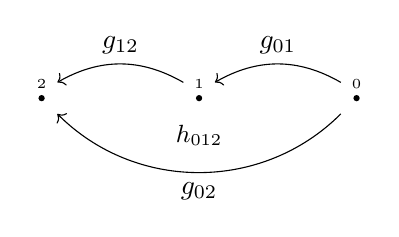
\begin{tikzpicture}[scale=2]
       \begin{scope}[xshift=0.0cm, yshift=0.0cm]
       \coordinate (0) at (0,0); 
 	\coordinate (1) at (-1,0); 
	 \coordinate (2) at (-2,0);
	 \draw (0) node[above] {\tiny0};
	 \draw (1) node[above] {\tiny1};
	 \draw (2) node[above] {\tiny 2};
 \fill[black] (0) circle[radius=0.02];
      \fill[black] (1) circle[radius=0.02];
      \fill[black] (2) circle[radius=0.02];
      \draw[<-] ($(1)+(0.1,0.1)$) to [out=30,in=150] node[midway] (g01) {} ($(0)+(-0.1,0.1)$)   ;
	      \node[above] at (g01) {$g_{01}$};
	\draw[<-] ($(2)+(0.1,0.1)$)to [out=30,in=150] node[midway] (g12) {} ($(1)+(-0.1,0.1)$)    ;
	      \node[above] at (g12) {$g_{12}$};     
	\draw[<-] ($(2)+(0.1,-0.1)$)to [out=-45,in=-135] node[midway] (g02) {} ($(0)+(-0.1,-0.1)$)    ;
	      \node[below] at (g02) {$g_{02}$};    
	 %\draw [line width=1pt, double distance=3pt, arrows = {-Latex[length=0pt 3 0]}]
        %($(1)-(0,-0.1)$) -- ($(g02) + (0, 0.1)$);    
        \draw ($(1)!0.5!(g02)$) node[] {\small $h_{012}$};    
    \end{scope}
  \end{tikzpicture}
\end{center}
\caption{Figure of $h_{012}$}
\label{d:h012}
\end{figure}

By using Figure~\ref{d:h012}, we can understand formulas~(\ref{r3-simplex m})-(\ref{r5-simplex m}) diagrammatically.
Formula~(\ref{r3-simplex m}) can be described as shown in Figure~\ref{d:l0123}.
\begin{figure}
\begin{center}
  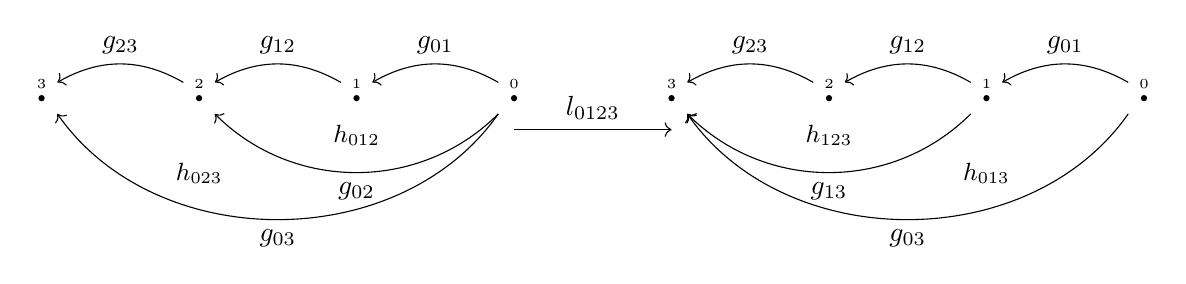
\begin{tikzpicture}[scale=2]
       \begin{scope}[xshift=0.0cm, yshift=0.0cm]
       \coordinate (0) at (0,0); 
 	\coordinate (1) at (-1,0); 
	 \coordinate (2) at (-2,0);
	 \coordinate (3) at (-3,0);
	 \draw (0) node[above] {\tiny0};
	 \draw (1) node[above] {\tiny1};
	 \draw (2) node[above] {\tiny 2};
	 \draw (3) node[above] {\tiny 3};
 \fill[black] (0) circle[radius=0.02];
      \fill[black] (1) circle[radius=0.02];
      \fill[black] (2) circle[radius=0.02];
       \fill[black] (3) circle[radius=0.02];
      \draw[<-] ($(1)+(0.1,0.1)$) to [out=30,in=150] node[midway] (g01) {} ($(0)+(-0.1,0.1)$)   ;
	      \node[above] at (g01) {$g_{01}$};
	\draw[<-] ($(2)+(0.1,0.1)$)to [out=30,in=150] node[midway] (g12) {} ($(1)+(-0.1,0.1)$)    ;
	      \node[above] at (g12) {$g_{12}$};  
	 \draw[<-] ($(3)+(0.1,0.1)$)to [out=30,in=150] node[midway] (g23) {} ($(2)+(-0.1,0.1)$)    ;
	      \node[above] at (g23) {$g_{23}$};             
	\draw[<-] ($(2)+(0.1,-0.1)$)to [out=-45,in=-135] node[midway] (g02) {} ($(0)+(-0.1,-0.1)$)    ;
	      \node[below] at (g02) {$g_{02}$};    
	      
	 %\draw [line width=1pt, double distance=3pt, arrows = {-Latex[length=0pt 3 0]}]
        %($(1)-(0,-0.1)$) -- ($(g02) + (0, 0.1)$);    
        \draw ($(1)!0.5!(g02)$) node[] {\small $h_{012}$};   
        
        \draw[<-] ($(3)+(0.1,-0.1)$)to [out=-55,in=-125] node[midway] (g03) {} ($(0)+(-0.1,-0.1)$)    ;
	      \node[below] at (g03) {$g_{03}$}; 
	      \draw ($(g03)!0.5!(g23)-(0,0.2)$) node[] {\small $h_{023}$};    
    \end{scope}
    \begin{scope}[xshift=4.0cm, yshift=0.0cm]
       \coordinate (0) at (0,0); 
 	\coordinate (1) at (-1,0); 
	 \coordinate (2) at (-2,0);
	 \coordinate (3) at (-3,0);
	 \draw (0) node[above] {\tiny0};
	 \draw (1) node[above] {\tiny1};
	 \draw (2) node[above] {\tiny 2};
	 \draw (3) node[above] {\tiny 3};
 \fill[black] (0) circle[radius=0.02];
      \fill[black] (1) circle[radius=0.02];
      \fill[black] (2) circle[radius=0.02];
       \fill[black] (3) circle[radius=0.02];
      \draw[<-] ($(1)+(0.1,0.1)$) to [out=30,in=150] node[midway] (g01) {} ($(0)+(-0.1,0.1)$)   ;
	      \node[above] at (g01) {$g_{01}$};
	\draw[<-] ($(2)+(0.1,0.1)$)to [out=30,in=150] node[midway] (g12) {} ($(1)+(-0.1,0.1)$)    ;
	      \node[above] at (g12) {$g_{12}$};  
	 \draw[<-] ($(3)+(0.1,0.1)$)to [out=30,in=150] node[midway] (g23) {} ($(2)+(-0.1,0.1)$)    ;
	      \node[above] at (g23) {$g_{23}$};             
	\draw[<-] ($(3)+(0.1,-0.1)$)to [out=-45,in=-135] node[midway] (g13) {} ($(1)+(-0.1,-0.1)$)    ;
	      \node[below] at (g13) {$g_{13}$};      
        \draw ($(2)!0.5!(g13)$) node[] {\small $h_{123}$};           
        \draw[<-] ($(3)+(0.1,-0.1)$)to [out=-55,in=-125] node[midway] (g03) {} ($(0)+(-0.1,-0.1)$)    ;
	      \node[below] at (g03) {$g_{03}$}; 
	      \draw ($(g03)!0.5!(g01)-(0,0.2)$) node[] {\small $h_{013}$};    
    \end{scope}
      \draw[->] (0,-0.2) to (1,-0.2);
      \node at (0.5,-0.2) [above]{$l_{0123}$};
  \end{tikzpicture}
\end{center}
\caption{Diagram of $l_{0123}$}
\label{d:l0123}
\end{figure}

We can interpret $l_{0123}$ as an operator that shifts the inner arch within the outer arch. Formula~\ref{r4-simplex m} can then be represented as in Figure~\ref{d:m01234}.
\begin{figure}[!]
\begin{center}
  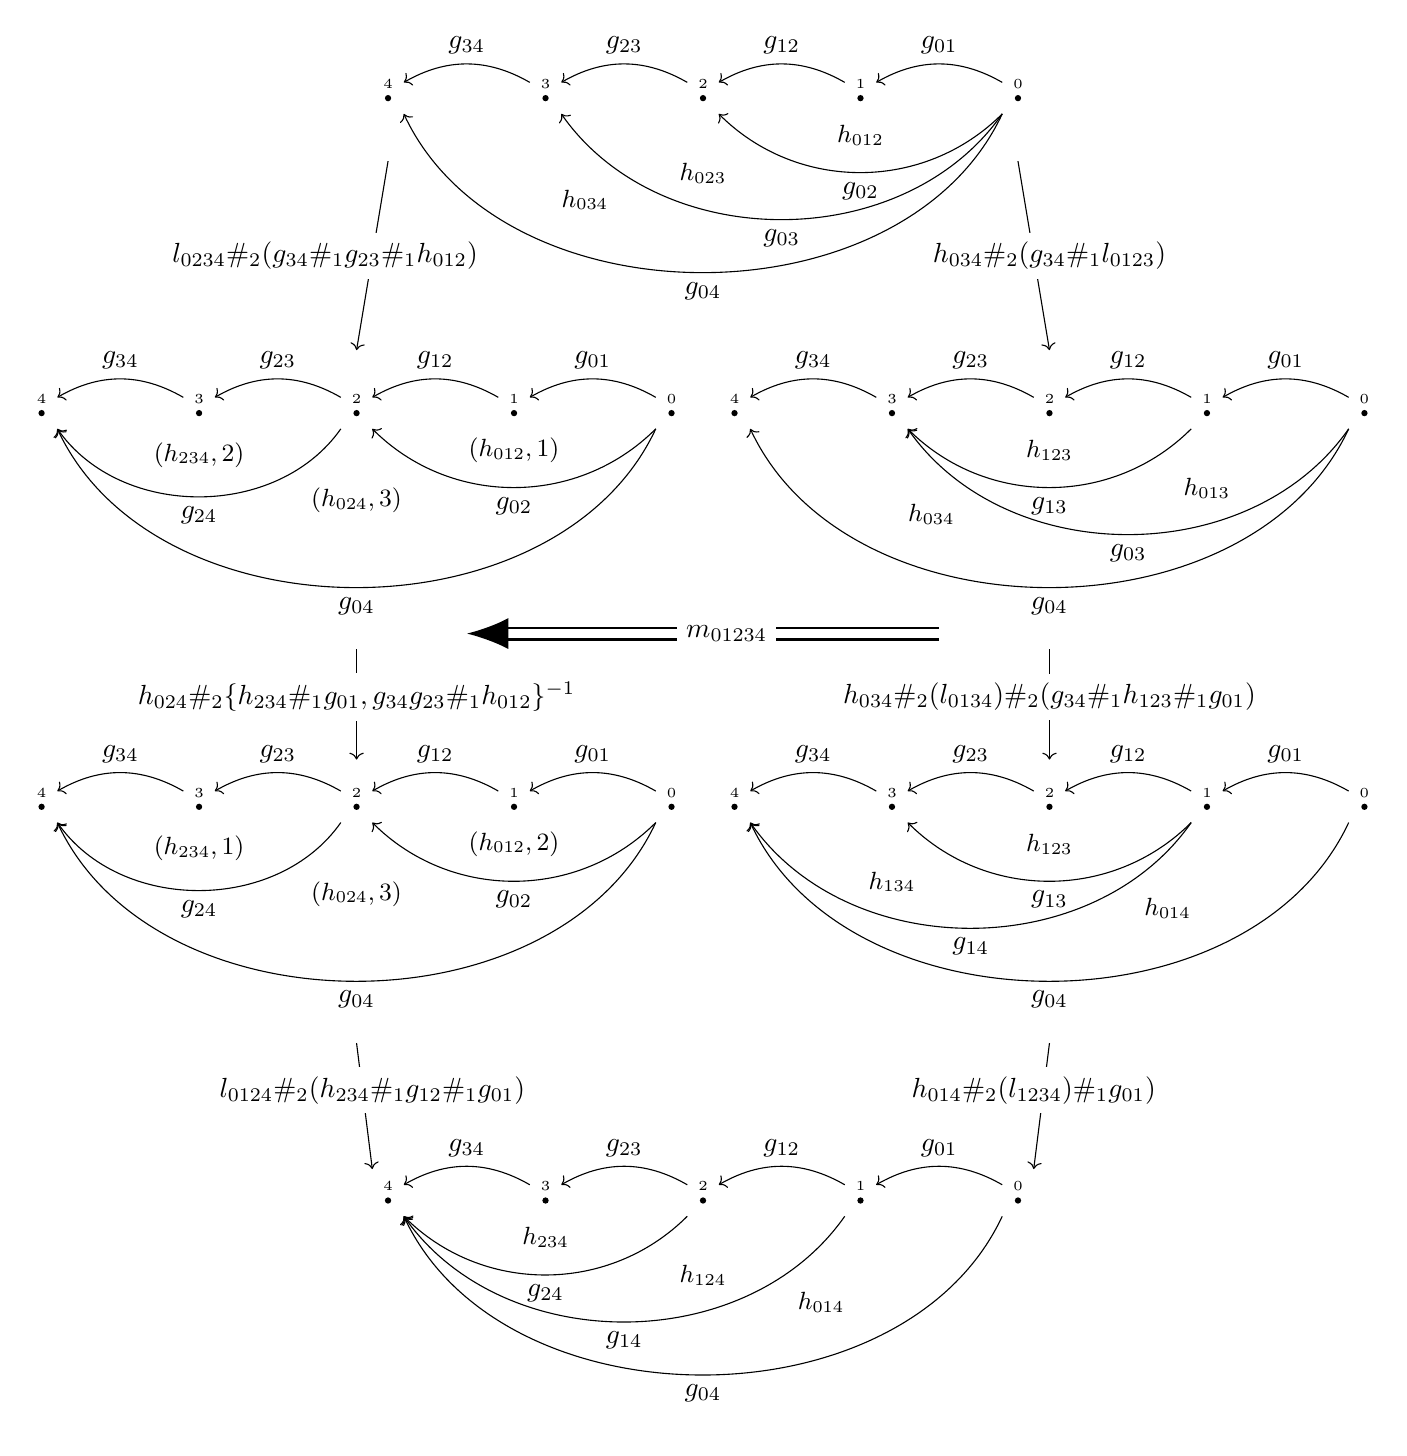
\begin{tikzpicture}[scale=2]
       \begin{scope}[xshift=0.0cm, yshift=0.0cm]
       \coordinate (0) at (0,0); 
 	\coordinate (1) at (-1,0); 
	 \coordinate (2) at (-2,0);
	 \coordinate (3) at (-3,0);
	  \coordinate (4) at (-4,0);
	 \draw (0) node[above] {\tiny0};
	 \draw (1) node[above] {\tiny1};
	 \draw (2) node[above] {\tiny 2};
	 \draw (3) node[above] {\tiny 3};
	 \draw (4) node[above] {\tiny 4};
 \fill[black] (0) circle[radius=0.02];
      \fill[black] (1) circle[radius=0.02];
      \fill[black] (2) circle[radius=0.02];
       \fill[black] (3) circle[radius=0.02];
       \fill[black] (4) circle[radius=0.02];
      \draw[<-] ($(1)+(0.1,0.1)$) to [out=30,in=150] node[midway] (g01) {} ($(0)+(-0.1,0.1)$)   ;
	      \node[above] at (g01) {$g_{01}$};
	\draw[<-] ($(2)+(0.1,0.1)$)to [out=30,in=150] node[midway] (g12) {} ($(1)+(-0.1,0.1)$)    ;
	      \node[above] at (g12) {$g_{12}$};  
	 \draw[<-] ($(3)+(0.1,0.1)$)to [out=30,in=150] node[midway] (g23) {} ($(2)+(-0.1,0.1)$)    ;
	      \node[above] at (g23) {$g_{23}$};  
	   \draw[<-] ($(4)+(0.1,0.1)$)to [out=30,in=150] node[midway] (g34) {} ($(3)+(-0.1,0.1)$)    ;
	      \node[above] at (g34) {$g_{34}$};                    
	\draw[<-] ($(2)+(0.1,-0.1)$)to [out=-45,in=-135] node[midway] (g02) {} ($(0)+(-0.1,-0.1)$)    ;
	      \node[below] at (g02) {$g_{02}$};  
	  \draw[<-] ($(3)+(0.1,-0.1)$)to [out=-55,in=-125] node[midway] (g03) {} ($(0)+(-0.1,-0.1)$)    ;
	      \node[below] at (g03) {$g_{03}$};     
	 \draw[<-] ($(4)+(0.1,-0.1)$)to [out=-65,in=-115] node[midway] (g04) {} ($(0)+(-0.1,-0.1)$)    ;
	      \node[below] at (g04) {$g_{04}$};        	      
	 %\draw [line width=1pt, double distance=3pt, arrows = {-Latex[length=0pt 3 0]}]
        %($(1)-(0,-0.1)$) -- ($(g02) + (0, 0.1)$);    
        \draw ($(1)!0.5!(g02)$) node[] {\small $h_{012}$};   
        \draw ($(g03)!0.5!(g23)-(0,0.2)$) node[] {\small $h_{023}$}; 
        \draw ($(g04)!0.5!(g34)-(0,0.2)$) node[] {\small $h_{034}$};          
    \end{scope}
    
     \begin{scope}[xshift=2.2cm, yshift=-2.0cm]
       \coordinate (0) at (0,0); 
 	\coordinate (1) at (-1,0); 
	 \coordinate (2) at (-2,0);
	 \coordinate (3) at (-3,0);
	  \coordinate (4) at (-4,0);
	 \draw (0) node[above] {\tiny0};
	 \draw (1) node[above] {\tiny1};
	 \draw (2) node[above] {\tiny 2};
	 \draw (3) node[above] {\tiny 3};
	 \draw (4) node[above] {\tiny 4};
 \fill[black] (0) circle[radius=0.02];
      \fill[black] (1) circle[radius=0.02];
      \fill[black] (2) circle[radius=0.02];
       \fill[black] (3) circle[radius=0.02];
       \fill[black] (4) circle[radius=0.02];
      \draw[<-] ($(1)+(0.1,0.1)$) to [out=30,in=150] node[midway] (g01) {} ($(0)+(-0.1,0.1)$)   ;
	      \node[above] at (g01) {$g_{01}$};
	\draw[<-] ($(2)+(0.1,0.1)$)to [out=30,in=150] node[midway] (g12) {} ($(1)+(-0.1,0.1)$)    ;
	      \node[above] at (g12) {$g_{12}$};  
	 \draw[<-] ($(3)+(0.1,0.1)$)to [out=30,in=150] node[midway] (g23) {} ($(2)+(-0.1,0.1)$)    ;
	      \node[above] at (g23) {$g_{23}$};  
	   \draw[<-] ($(4)+(0.1,0.1)$)to [out=30,in=150] node[midway] (g34) {} ($(3)+(-0.1,0.1)$)    ;
	      \node[above] at (g34) {$g_{34}$};                    
	\draw[<-] ($(3)+(0.1,-0.1)$)to [out=-45,in=-135] node[midway] (g13) {} ($(1)+(-0.1,-0.1)$)    ;
	      \node[below] at (g13) {$g_{13}$};  
	  \draw[<-] ($(3)+(0.1,-0.1)$)to [out=-55,in=-125] node[midway] (g03) {} ($(0)+(-0.1,-0.1)$)    ;
	      \node[below] at (g03) {$g_{03}$};     
	 \draw[<-] ($(4)+(0.1,-0.1)$)to [out=-65,in=-115] node[midway] (g04) {} ($(0)+(-0.1,-0.1)$)    ;
	      \node[below] at (g04) {$g_{04}$};        	      
	 %\draw [line width=1pt, double distance=3pt, arrows = {-Latex[length=0pt 3 0]}]
        %($(1)-(0,-0.1)$) -- ($(g02) + (0, 0.1)$);    
        \draw ($(2)!0.5!(g13)$) node[] {\small $h_{123}$};   
        \draw ($(g03)!0.5!(g01)-(0,0.2)$) node[] {\small $h_{013}$}; 
        \draw ($(g04)!0.5!(g34)-(0,0.2)$) node[] {\small $h_{034}$};          
    \end{scope}
    
    \begin{scope}[xshift=2.2cm, yshift=-4.5cm]
       \coordinate (0) at (0,0); 
 	\coordinate (1) at (-1,0); 
	 \coordinate (2) at (-2,0);
	 \coordinate (3) at (-3,0);
	  \coordinate (4) at (-4,0);
	 \draw (0) node[above] {\tiny0};
	 \draw (1) node[above] {\tiny1};
	 \draw (2) node[above] {\tiny 2};
	 \draw (3) node[above] {\tiny 3};
	 \draw (4) node[above] {\tiny 4};
 \fill[black] (0) circle[radius=0.02];
      \fill[black] (1) circle[radius=0.02];
      \fill[black] (2) circle[radius=0.02];
       \fill[black] (3) circle[radius=0.02];
       \fill[black] (4) circle[radius=0.02];
      \draw[<-] ($(1)+(0.1,0.1)$) to [out=30,in=150] node[midway] (g01) {} ($(0)+(-0.1,0.1)$)   ;
	      \node[above] at (g01) {$g_{01}$};
	\draw[<-] ($(2)+(0.1,0.1)$)to [out=30,in=150] node[midway] (g12) {} ($(1)+(-0.1,0.1)$)    ;
	      \node[above] at (g12) {$g_{12}$};  
	 \draw[<-] ($(3)+(0.1,0.1)$)to [out=30,in=150] node[midway] (g23) {} ($(2)+(-0.1,0.1)$)    ;
	      \node[above] at (g23) {$g_{23}$};  
	   \draw[<-] ($(4)+(0.1,0.1)$)to [out=30,in=150] node[midway] (g34) {} ($(3)+(-0.1,0.1)$)    ;
	      \node[above] at (g34) {$g_{34}$};                    
	\draw[<-] ($(3)+(0.1,-0.1)$)to [out=-45,in=-135] node[midway] (g13) {} ($(1)+(-0.1,-0.1)$)    ;
	      \node[below] at (g13) {$g_{13}$};  
	  \draw[<-] ($(4)+(0.1,-0.1)$)to [out=-55,in=-125] node[midway] (g14) {} ($(1)+(-0.1,-0.1)$)    ;
	      \node[below] at (g14) {$g_{14}$};     
	 \draw[<-] ($(4)+(0.1,-0.1)$)to [out=-65,in=-115] node[midway] (g04) {} ($(0)+(-0.1,-0.1)$)    ;
	      \node[below] at (g04) {$g_{04}$};        	      
	 %\draw [line width=1pt, double distance=3pt, arrows = {-Latex[length=0pt 3 0]}]
        %($(1)-(0,-0.1)$) -- ($(g02) + (0, 0.1)$);    
        \draw ($(2)!0.5!(g13)$) node[] {\small $h_{123}$};   
        \draw ($(g14)!0.5!(g34)-(0,0.2)$) node[] {\small $h_{134}$}; 
        \draw ($(g04)!0.5!(g01)-(0,0.2)$) node[] {\small $h_{014}$};          
    \end{scope}
    
    \begin{scope}[xshift=0.0cm, yshift=-7.0cm]
       \coordinate (0) at (0,0); 
 	\coordinate (1) at (-1,0); 
	 \coordinate (2) at (-2,0);
	 \coordinate (3) at (-3,0);
	  \coordinate (4) at (-4,0);
	 \draw (0) node[above] {\tiny0};
	 \draw (1) node[above] {\tiny1};
	 \draw (2) node[above] {\tiny 2};
	 \draw (3) node[above] {\tiny 3};
	 \draw (4) node[above] {\tiny 4};
 \fill[black] (0) circle[radius=0.02];
      \fill[black] (1) circle[radius=0.02];
      \fill[black] (2) circle[radius=0.02];
       \fill[black] (3) circle[radius=0.02];
       \fill[black] (4) circle[radius=0.02];
      \draw[<-] ($(1)+(0.1,0.1)$) to [out=30,in=150] node[midway] (g01) {} ($(0)+(-0.1,0.1)$)   ;
	      \node[above] at (g01) {$g_{01}$};
	\draw[<-] ($(2)+(0.1,0.1)$)to [out=30,in=150] node[midway] (g12) {} ($(1)+(-0.1,0.1)$)    ;
	      \node[above] at (g12) {$g_{12}$};  
	 \draw[<-] ($(3)+(0.1,0.1)$)to [out=30,in=150] node[midway] (g23) {} ($(2)+(-0.1,0.1)$)    ;
	      \node[above] at (g23) {$g_{23}$};  
	   \draw[<-] ($(4)+(0.1,0.1)$)to [out=30,in=150] node[midway] (g34) {} ($(3)+(-0.1,0.1)$)    ;
	      \node[above] at (g34) {$g_{34}$};                    
	\draw[<-] ($(4)+(0.1,-0.1)$)to [out=-45,in=-135] node[midway] (g24) {} ($(2)+(-0.1,-0.1)$)    ;
	      \node[below] at (g24) {$g_{24}$};  
	  \draw[<-] ($(4)+(0.1,-0.1)$)to [out=-55,in=-125] node[midway] (g14) {} ($(1)+(-0.1,-0.1)$)    ;
	      \node[below] at (g14) {$g_{14}$};     
	 \draw[<-] ($(4)+(0.1,-0.1)$)to [out=-65,in=-115] node[midway] (g04) {} ($(0)+(-0.1,-0.1)$)    ;
	      \node[below] at (g04) {$g_{04}$};        	      
	 %\draw [line width=1pt, double distance=3pt, arrows = {-Latex[length=0pt 3 0]}]
        %($(1)-(0,-0.1)$) -- ($(g02) + (0, 0.1)$);    
        \draw ($(3)!0.5!(g24)$) node[] {\small $h_{234}$};   
        \draw ($(g14)!0.5!(g12)-(0,0.2)$) node[] {\small $h_{124}$}; 
        \draw ($(g04)!0.5!(g01)-(0,0.2)$) node[] {\small $h_{014}$};          
    \end{scope}
    
     \begin{scope}[xshift=-2.2cm, yshift=-2.0cm]
       \coordinate (0) at (0,0); 
 	\coordinate (1) at (-1,0); 
	 \coordinate (2) at (-2,0);
	 \coordinate (3) at (-3,0);
	  \coordinate (4) at (-4,0);
	 \draw (0) node[above] {\tiny0};
	 \draw (1) node[above] {\tiny1};
	 \draw (2) node[above] {\tiny 2};
	 \draw (3) node[above] {\tiny 3};
	 \draw (4) node[above] {\tiny 4};
 \fill[black] (0) circle[radius=0.02];
      \fill[black] (1) circle[radius=0.02];
      \fill[black] (2) circle[radius=0.02];
       \fill[black] (3) circle[radius=0.02];
       \fill[black] (4) circle[radius=0.02];
      \draw[<-] ($(1)+(0.1,0.1)$) to [out=30,in=150] node[midway] (g01) {} ($(0)+(-0.1,0.1)$)   ;
	      \node[above] at (g01) {$g_{01}$};
	\draw[<-] ($(2)+(0.1,0.1)$)to [out=30,in=150] node[midway] (g12) {} ($(1)+(-0.1,0.1)$)    ;
	      \node[above] at (g12) {$g_{12}$};  
	 \draw[<-] ($(3)+(0.1,0.1)$)to [out=30,in=150] node[midway] (g23) {} ($(2)+(-0.1,0.1)$)    ;
	      \node[above] at (g23) {$g_{23}$};  
	   \draw[<-] ($(4)+(0.1,0.1)$)to [out=30,in=150] node[midway] (g34) {} ($(3)+(-0.1,0.1)$)    ;
	      \node[above] at (g34) {$g_{34}$};                    
	\draw[<-] ($(2)+(0.1,-0.1)$)to [out=-45,in=-135] node[midway] (g02) {} ($(0)+(-0.1,-0.1)$)    ;
	      \node[below] at (g02) {$g_{02}$};  
	  \draw[<-] ($(4)+(0.1,-0.1)$)to [out=-55,in=-125] node[midway] (g24) {} ($(2)+(-0.1,-0.1)$)    ;
	      \node[below] at (g24) {$g_{24}$};     
	 \draw[<-] ($(4)+(0.1,-0.1)$)to [out=-65,in=-115] node[midway] (g04) {} ($(0)+(-0.1,-0.1)$)    ;
	      \node[below] at (g04) {$g_{04}$};        	      
	 %\draw [line width=1pt, double distance=3pt, arrows = {-Latex[length=0pt 3 0]}]
        %($(1)-(0,-0.1)$) -- ($(g02) + (0, 0.1)$);    
        \draw ($(1)!0.5!(g02)$) node[] {\small $(h_{012},1)$};   
        \draw ($(3)!0.5!(g24)$) node[] {\small $(h_{234},2)$}; 
        \draw ($(g04)!0.5!(2)$) node[] {\small $(h_{024},3)$};          
    \end{scope}
    
    \begin{scope}[xshift=-2.2cm, yshift=-4.5cm]
       \coordinate (0) at (0,0); 
 	\coordinate (1) at (-1,0); 
	 \coordinate (2) at (-2,0);
	 \coordinate (3) at (-3,0);
	  \coordinate (4) at (-4,0);
	 \draw (0) node[above] {\tiny0};
	 \draw (1) node[above] {\tiny1};
	 \draw (2) node[above] {\tiny 2};
	 \draw (3) node[above] {\tiny 3};
	 \draw (4) node[above] {\tiny 4};
 \fill[black] (0) circle[radius=0.02];
      \fill[black] (1) circle[radius=0.02];
      \fill[black] (2) circle[radius=0.02];
       \fill[black] (3) circle[radius=0.02];
       \fill[black] (4) circle[radius=0.02];
      \draw[<-] ($(1)+(0.1,0.1)$) to [out=30,in=150] node[midway] (g01) {} ($(0)+(-0.1,0.1)$)   ;
	      \node[above] at (g01) {$g_{01}$};
	\draw[<-] ($(2)+(0.1,0.1)$)to [out=30,in=150] node[midway] (g12) {} ($(1)+(-0.1,0.1)$)    ;
	      \node[above] at (g12) {$g_{12}$};  
	 \draw[<-] ($(3)+(0.1,0.1)$)to [out=30,in=150] node[midway] (g23) {} ($(2)+(-0.1,0.1)$)    ;
	      \node[above] at (g23) {$g_{23}$};  
	   \draw[<-] ($(4)+(0.1,0.1)$)to [out=30,in=150] node[midway] (g34) {} ($(3)+(-0.1,0.1)$)    ;
	      \node[above] at (g34) {$g_{34}$};                    
	\draw[<-] ($(2)+(0.1,-0.1)$)to [out=-45,in=-135] node[midway] (g02) {} ($(0)+(-0.1,-0.1)$)    ;
	      \node[below] at (g02) {$g_{02}$};  
	  \draw[<-] ($(4)+(0.1,-0.1)$)to [out=-55,in=-125] node[midway] (g24) {} ($(2)+(-0.1,-0.1)$)    ;
	      \node[below] at (g24) {$g_{24}$};     
	 \draw[<-] ($(4)+(0.1,-0.1)$)to [out=-65,in=-115] node[midway] (g04) {} ($(0)+(-0.1,-0.1)$)    ;
	      \node[below] at (g04) {$g_{04}$};        	      
	 %\draw [line width=1pt, double distance=3pt, arrows = {-Latex[length=0pt 3 0]}]
        %($(1)-(0,-0.1)$) -- ($(g02) + (0, 0.1)$);    
        \draw ($(1)!0.5!(g02)$) node[] {\small $(h_{012},2)$};   
        \draw ($(3)!0.5!(g24)$) node[] {\small $(h_{234},1)$}; 
        \draw ($(g04)!0.5!(2)$) node[] {\small $(h_{024},3)$};          
    \end{scope}
    \draw[->] (-0.0,-0.4) to (0.2,-1.6);
      \node at (0.2,-1.0) [fill=white]{$h_{034} \#_2(g_{34} \#_1 l_{0123})$};
      \draw[->] (0.2,-3.5) to (0.2,-4.2);
      \node at (0.2,-3.8) [fill=white]{$h_{034} \#_2( l_{0134})\#_2 (g_{34}\#_1 h_{123} \#_1 g_{01})$};
      \draw[->] (0.2,-6.0) to (0.1,-6.8);
      \node at (0.1,-6.3) [fill=white]{$h_{014} \#_2( l_{1234})\#_1 g_{01}) $};
      
      \draw[->] (-4.0,-0.4) to (-4.2,-1.6);
      \node at (-4.4,-1.0) [fill=white]{$l_{0234}\#_2 (g_{34} \#_1 g_{23}\#_1 h_{012})$};
      \draw[->] (-4.2,-3.5) to (-4.2,-4.2);
      \node at (-4.2,-3.8) [fill=white]{$ h_{024}\#_2 \{h_{234}\#_1 g_{01} , g_{34}g_{23}\#_1 h_{012}\}^{-1}$};
      \draw[->] (-4.2,-6.0) to (-4.1,-6.8);
      \node at (-4.1,-6.3) [fill=white]{$l_{0124} \#_2 (h_{234}\#_1 g_{12} \#_1 g_{01}) $};
      
      \draw [line width=1pt, double distance=3pt, arrows = {-Latex[length=0pt 3 0]}]
         (-0.5, -3.4)-- (-3.5, -3.4) ;
      \node at ($(-3.5, -3.4)!0.55!(-0.5, -3.4)$)  [fill=white]{$m_{01234}$};
  \end{tikzpicture}
\end{center}
\caption{Diagram of $m_{01234}$}
\label{d:m01234}
\end{figure}

Formula~(\ref{r5-simplex m:eq}) can also be represented diagrammatically. Figure~\ref{d:5simp-lhs} illustrates the left-hand side of~(\ref{r5-simplex m:eq}) while Figure~\ref{d:5simp-rhs} illustrates the right-hand side.
\begin{figure}[!]
\begin{center}
  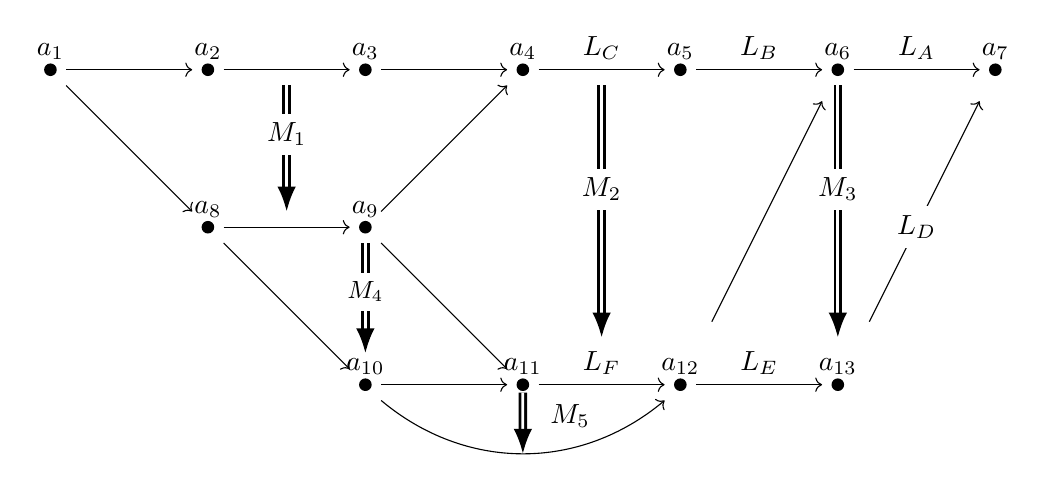
\begin{tikzpicture}[scale=2] 
	\coordinate (a1) at (0,0); 
	\coordinate (a2) at (1,0); 
	\coordinate (a3) at (2,0);
	\coordinate (a4) at (3,0);
	\coordinate (a5) at (4,0);
	\coordinate (a6) at (5,0);
	\coordinate (a7) at (6,0);
	\coordinate (a8) at (1,-1);
	\coordinate (a9) at (2,-1);
	\coordinate (a10) at (2,-2);
	\coordinate (a11) at (3,-2);
	\coordinate (a12) at (4,-2);
	\coordinate (a13) at (5,-2);
	\fill (a1) circle [radius=0.04] node[above] {$a_1$};
	\fill (a2) circle [radius=0.04] node[above] {$a_2$};
	\fill (a3) circle [radius=0.04] node[above] {$a_3$};
	\fill (a4) circle [radius=0.04] node[above] {$a_4$};
	\fill (a5) circle [radius=0.04] node[above] {$a_5$};
	\fill (a6) circle [radius=0.04] node[above] {$a_6$};
	\fill (a7) circle [radius=0.04] node[above] {$a_7$};
	\fill (a8) circle [radius=0.04] node[above] {$a_8$};
	\fill (a9) circle [radius=0.04] node[above] {$a_9$};
	\fill (a10) circle [radius=0.04] node[above] {$a_{10}$};
	\fill (a11) circle [radius=0.04] node[above] {$a_{11}$};
	\fill (a12) circle [radius=0.04] node[above] {$a_{12}$};
	\fill (a13) circle [radius=0.04] node[above] {$a_{13}$};
	
	\draw[->] ($(a1)+(0.1,0)$) to ($(a2)-(0.1,0)$);
	\draw[->] ($(a2)+(0.1,0)$) to ($(a3)-(0.1,0)$);
	\draw[->] ($(a3)+(0.1,0)$) to ($(a4)-(0.1,0)$);
	\draw[->] ($(a4)+(0.1,0)$) to ($(a5)-(0.1,0)$);
	\draw[->] ($(a5)+(0.1,0)$) to ($(a6)-(0.1,0)$);
	\draw[->] ($(a6)+(0.1,0)$) to ($(a7)-(0.1,0)$);
	
	\draw[->] ($(a1)+(0.1,-0.1)$) to ($(a8)-(0.1,-0.1)$);
	\draw[->] ($(a8)+(0.1,0)$) to ($(a9)-(0.1,0)$);
	\draw[->] ($(a9)+(0.1,0.1)$) to ($(a4)-(0.1,0.1)$);
	
	\draw[->] ($(a8)+(0.1,-0.1)$) to ($(a10)-(0.1,-0.1)$);
	\draw[->] ($(a9)+(0.1,-0.1)$) to ($(a11)-(0.1,-0.1)$);
	\draw[->] ($(a10)+(0.1,0)$) to ($(a11)-(0.1,0)$);
	\draw[->] ($(a11)+(0.1,0)$) to ($(a12)-(0.1,0)$);
	\draw[->] ($(a12)+(0.1,0)$) to ($(a13)-(0.1,0)$);
	\draw[->] ($(a12)+(0.2,0.4)$) to ($(a6)-(0.1,0.2)$);
	\draw[->] ($(a13)+(0.2,0.4)$) to ($(a7)-(0.1,0.2)$);
	\draw[->] ($(a10)-(-0.1,0.1)$) to [out=-40,in=-140] node[midway] (a10-a12) {} ($(a12)-(0.1,0.1)$)   ;
	
	\node[above] at ($(a6)!0.5!(a7)$) {$L_{A}$}; 
	\node[above] at ($(a5)!0.5!(a6)$) {$L_{B}$};
	\node[above] at ($(a4)!0.5!(a5)$) {$L_{C}$};
	\node[fill=white] at ($(a7)!0.5!(a13)$) {$L_{D}$};
	\node[above] at ($(a12)!0.5!(a13)$) {$L_{E}$};
	\node[above] at ($(a11)!0.5!(a12)$) {$L_{F}$};
	
	\draw [line width=1pt, double distance=1pt, arrows = {-Latex[length=0pt 3 0]}]
         ($(a2)!0.5!(a3) + (0,-0.1)$)-- ($(a8)!0.5!(a9)+ (0,0.1)$);
      \node at ($($(a2)!0.5!(a3) + (0,-0.2)$)!0.35!($(a8)!0.5!(a9)+ (0,0.2)$)$)  [fill=white]{$M_{1}$};
      \draw [line width=1pt, double distance=1pt, arrows = {-Latex[length=0pt 3 0]}]
         ($(a4)!0.5!(a5) + (0,-0.1)$)-- ($(a11)!0.5!(a12)+ (0,0.3)$);
      \node at ($($(a4)!0.5!(a5) + (0,-0.2)$)!0.35!($(a11)!0.5!(a12)+ (0,0.2)$)$)  [fill=white]{$M_{2}$};
      \draw [line width=1pt, double distance=1pt, arrows = {-Latex[length=0pt 3 0]}]
         ($(a6) + (0,-0.1)$)-- ($(a13)+ (0,0.3)$);
      \node at ($($(a6) + (0,-0.2)$)!0.35!($(a13)+ (0,0.2)$)$)  [fill=white]{$M_{3}$};
      \draw [line width=1pt, double distance=1pt, arrows = {-Latex[length=0pt 3 0]}]
         ($(a9) + (0,-0.1)$)-- ($(a10)+ (0,0.2)$);
      \node at ($($(a9) + (0,-0.2)$)!0.35!($(a10)+ (0,0.2)$)$)  [fill=white]{\small $ M_{4}$};
      \draw [line width=1pt, double distance=1pt, arrows = {-Latex[length=0pt 3 0]}]
         ($(a11) + (0,-0.05)$)-- ($(a10-a12)+ (0,0)$);
      \node at ($(a11)+(0.3,-0.2)$)  []{$ M_{5}$};
  \end{tikzpicture}
\end{center}
\caption{Diagram of left hand side of (\ref{r5-simplex m:eq}) }
\label{d:5simp-lhs}
  \end{figure}


\begin{figure}[!]
\begin{center}
  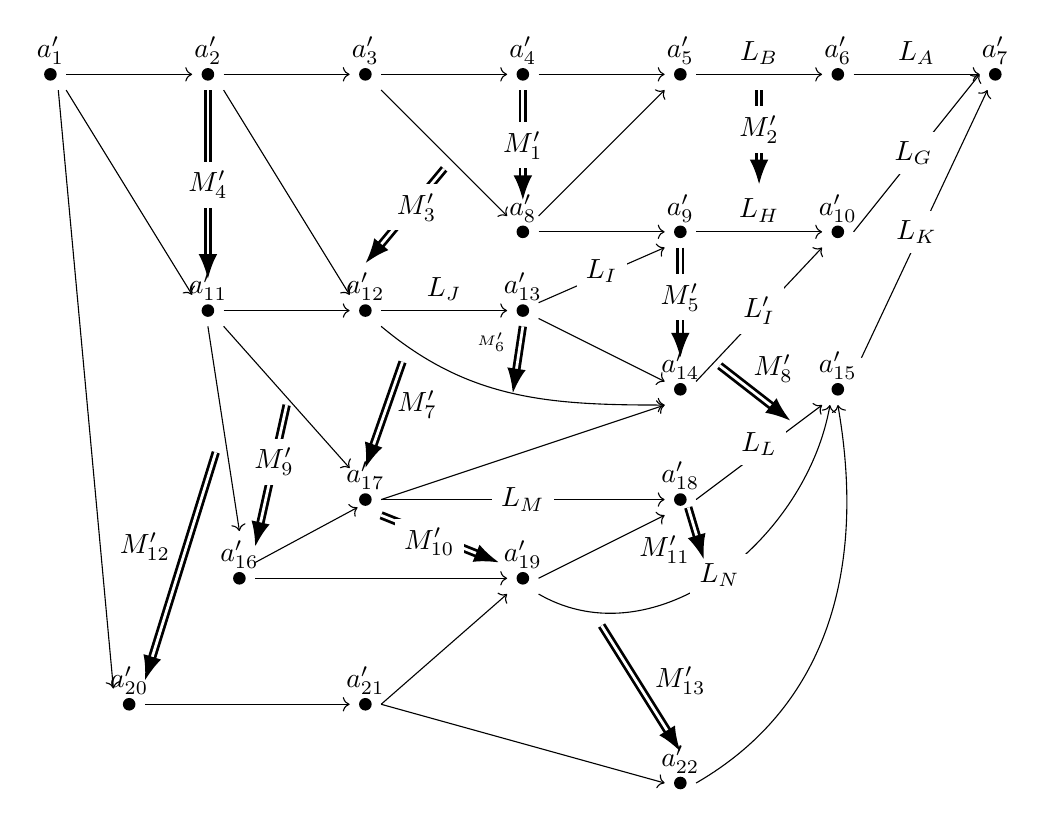
\begin{tikzpicture}[scale=2] 
	\coordinate (a1) at (0,0); 
	\coordinate (a2) at (1,0); 
	\coordinate (a3) at (2,0);
	\coordinate (a4) at (3,0);
	\coordinate (a5) at (4,0);
	\coordinate (a6) at (5,0);
	\coordinate (a7) at (6,0);
	%-------
	\coordinate (a8) at (3,-1);
	\coordinate (a9) at (4,-1);
	\coordinate (a10) at (5,-1);
	
	\coordinate (a11) at (1,-1.5);
	\coordinate (a12) at (2,-1.5);
	\coordinate (a13) at (3,-1.5);
	\coordinate (a14) at (4,-2);
	\coordinate (a15) at (5,-2);
	
	\coordinate (a16) at (1.2,-3.2);
	\coordinate (a17) at (2,-2.7);
	\coordinate (a18) at (4,-2.7);
	\coordinate (a19) at (3,-3.2);
	
	\coordinate (a20) at (0.5,-4);
	\coordinate (a21) at (2,-4);
	%\coordinate (a22) at (3,-4.5);
	\coordinate (a22) at (4,-4.5);
	
	\fill (a1) circle [radius=0.04] node[above] {$a'_1$};
	\fill (a2) circle [radius=0.04] node[above] {$a'_2$};
	\fill (a3) circle [radius=0.04] node[above] {$a'_3$};
	\fill (a4) circle [radius=0.04] node[above] {$a'_4$};
	\fill (a5) circle [radius=0.04] node[above] {$a'_5$};
	\fill (a6) circle [radius=0.04] node[above] {$a'_6$};
	\fill (a7) circle [radius=0.04] node[above] {$a'_7$};
	\fill (a8) circle [radius=0.04] node[above] {$a'_8$};
	\fill (a9) circle [radius=0.04] node[above] {$a'_9$};
	\fill (a10) circle [radius=0.04] node[above] {$a'_{10}$};
	\fill (a11) circle [radius=0.04] node[above] {$a'_{11}$};
	\fill (a12) circle [radius=0.04] node[above] {$a'_{12}$};
	\fill (a13) circle [radius=0.04] node[above] {$a'_{13}$};
	\fill (a14) circle [radius=0.04] node[above] {$a'_{14}$};
	\fill (a15) circle [radius=0.04] node[above] {$a'_{15}$};
	\fill (a16) circle [radius=0.04] node[above] {$a'_{16}$};
	\fill (a17) circle [radius=0.04] node[above] {$a'_{17}$};
	\fill (a18) circle [radius=0.04] node[above] {$a'_{18}$};
	\fill (a19) circle [radius=0.04] node[above] {$a'_{19}$};
	\fill (a20) circle [radius=0.04] node[above] {$a'_{20}$};
	\fill (a21) circle [radius=0.04] node[above] {$a'_{21}$};
	%\fill (a22) circle [radius=0.04] node[above] {$a_{22}$};
	\fill (a22) circle [radius=0.04] node[above] {$a'_{22}$};
	
	\draw[->] ($(a1)+(0.1,0)$) to ($(a2)-(0.1,0)$);
	\draw[->] ($(a2)+(0.1,0)$) to ($(a3)-(0.1,0)$);
	\draw[->] ($(a3)+(0.1,0)$) to ($(a4)-(0.1,0)$);
	\draw[->] ($(a4)+(0.1,0)$) to ($(a5)-(0.1,0)$);
	\draw[->] ($(a5)+(0.1,0)$) to ($(a6)-(0.1,0)$);
	\draw[->] ($(a6)+(0.1,0)$) to ($(a7)-(0.1,0)$);
	\draw[->] ($(a3)+(0.1,-0.1)$) to ($(a8)-(0.1,-0.1)$);
	\draw[->] ($(a8)+(0.1,0.1)$) to ($(a5)-(0.1,0.1)$);
	\draw[->] ($(a8)+(0.1,0)$) to ($(a9)-(0.1,0)$);
	\draw[->] ($(a9)+(0.1,0)$) to ($(a10)-(0.1,0)$);
	\draw[->] ($(a10)+(0.1,0)$) to ($(a7)-(0.1,0)$);
	
	\draw[->] ($(a1)+(0.1,-0.1)$) to ($(a11)-(0.1,-0.1)$);
	\draw[->] ($(a2)+(0.1,-0.1)$) to ($(a12)-(0.1,-0.1)$);
	\draw[->] ($(a11)+(0.1,-0)$) to ($(a12)-(0.1,-0)$);
	\draw[->] ($(a12)+(0.1,-0)$) to ($(a13)-(0.1,-0)$);
	\draw[->] ($(a13)+(0.1,0.05)$) to ($(a9)-(0.1,0.1)$);
	\draw[->] ($(a13)+(0.1,-0.05)$) to ($(a14)-(0.1,-0.05)$);
	\draw[->] ($(a14)+(0.1,0.05)$) to ($(a10)-(0.1,0.1)$);
	\draw[->] ($(a15)+(0.15,0.2)$) to ($(a7)-(0.05,0.1)$);
	
	\draw[->] ($(a12)-(-0.1,0.1)$) to [out=-40,in=-180] node[midway] (a12-a14) {} ($(a14)-(0.1,0.1)$);
	
	\draw[->] ($(a11)+(0,-0.1)$) to ($(a16)-(0.0,-0.3)$);
	\draw[->] ($(a11)+(0.1,-0.1)$) to ($(a17)-(0.1,-0.2)$);
	\draw[->] ($(a16)+(0.1,0.1)$) to ($(a17)-(0.05,0.05)$);
	\draw[->] ($(a17)+(0.1,-0)$) to ($(a18)-(0.1,-0)$);
	\draw[->] ($(a17)+(0.1,0)$) to ($(a14)-(0.1,0.1)$);
	\draw[->] ($(a16)+(0.1,-0)$) to ($(a19)-(0.1,-0)$);
	\draw[->] ($(a19)+(0.1,-0)$) to ($(a18)-(0.1,0.1)$);
	\draw[->] ($(a18)+(0.1,-0)$) to ($(a15)-(0.1,0.1)$);
	\draw[->] ($(a1)+(0.05,-0.1)$) to ($(a20)-(0.1,-0.1)$);
	\draw[->] ($(a20)+(0.1,0)$) to ($(a21)-(0.1,-0)$);
	\draw[->] ($(a21)+(0.1,0)$) to ($(a19)-(0.1,0.1)$);
	\draw[->] ($(a21)+(0.1,0)$) to ($(a22)-(0.1,0)$);
	%\draw[->] ($(a21)+(0.1,-0.05)$) to ($(a22)-(0.1,-0.1)$);
	%\draw[->] ($(a22)+(0.1,0)$) to ($(a23)-(0.1,-0)$);
	
	\draw[->] ($(a19)-(-0.1,0.1)$) to [out=-30,in=-100] node[midway] (a19-a15) {} ($(a15)-(0.05,0.1)$);
	\draw[->] ($(a22)-(-0.1,0)$) to [out=30,in=-80] node[midway] (a22-a15) {} ($(a15)-(0,0.1)$);
	%\draw[->] ($(a21)-(-0.1,0.02)$) to [out=20,in=120] node[midway] (a12-a14) {} ($(a23)-(0.1,-0.05)$);
	
	\node[above] at ($(a6)!0.5!(a7)$) {$L_{A}$}; 
	\node[above] at ($(a5)!0.5!(a6)$) {$L_{B}$};
	\node[fill=white] at ($(a7)!0.5!(a10)+(-0.02,0)$) {$L_{G}$};
	\node[above] at ($(a9)!0.5!(a10)$) {$L_{H}$};
	\node[fill=white] at ($(a13)!0.5!(a9)$) {$L_{I}$};
	\node[fill=white] at ($(a10)!0.5!(a14)$) {$L'_{I}$};
	\node[above] at ($(a12)!0.5!(a13)$) {$L_{J}$};
	\node[fill=white] at ($(a7)!0.5!(a15)$) {$L_{K}$};
	\node[fill=white] at ($(a15)!0.5!(a18)$) {$L_{L}$};
	\node[fill=white] at ($(a17)!0.5!(a18)$) {$L_{M}$};
	\node[fill=white] at ($(a19-a15)$) {$L_{N}$};
	
	
	\draw [line width=1pt, double distance=1pt, arrows = {-Latex[length=0pt 3 0]}]
         ($(a4) + (0,-0.1)$)-- ($(a8)+ (0,0.2)$);
      \node at ($($(a4) + (0,-0.1)$)!0.5!($(a8)+ (0,0.2)$)$)  [fill=white]{$M'_{1}$};
      \draw [line width=1pt, double distance=1pt, arrows = {-Latex[length=0pt 3 0]}]
         ($($(a5)!0.5!(a6)$)+ (0,-0.1)$)-- ($($(a9)!0.5!(a10)$)+ (0,0.3)$);
      \node at ($($($(a5)!0.5!(a6)$) + (0,-0.1)$)!0.5!($($(a9)!0.5!(a10)$)+ (0,0.4)$)$)  [fill=white]{$M'_{2}$};    
      \draw [line width=1pt, double distance=1pt, arrows = {-Latex[length=0pt 3 0]}]
         ($($(a3)!0.5!(a8)$)+ (0,-0.1)$)-- ($(a12)+ (0,0.3)$);
      \node at ($($($(a3)!0.5!(a8)$) + (0,-0.1)$)!0.35!($(a12)+ (0,0.2)$)$)  [fill=white]{$M'_{3}$};  
	\draw [line width=1pt, double distance=1pt, arrows = {-Latex[length=0pt 3 0]}]
         ($(a2) + (0,-0.1)$)-- ($(a11)+ (0,0.2)$);
      \node at ($($(a2) + (0,-0.1)$)!0.5!($(a11)+ (0,0.2)$)$)  [fill=white]{$M'_{4}$};
      \draw [line width=1pt, double distance=1pt, arrows = {-Latex[length=0pt 3 0]}]
         ($(a9) + (0,-0.1)$)-- ($(a14)+ (0,0.2)$);
      \node at ($($(a9) + (0,-0.1)$)!0.45!($(a14)+ (0,0.2)$)$)  [fill=white]{$M'_{5}$};
      \draw [line width=1pt, double distance=1pt, arrows = {-Latex[length=0pt 3 0]}]
         ($(a13) + (0,-0.1)$)-- ($(a12-a14)+ (0,0)$);
      \node at ($(a13) + (-0.2,-0.2)$)  []{\tiny $M'_{6}$};
       \node at ($($(a9) + (0,-0.1)$)!0.45!($(a14)+ (0,0.2)$)$)  [fill=white]{$M'_{5}$};
      \draw [line width=1pt, double distance=1pt, arrows = {-Latex[length=0pt 3 0]}]
         ($(a12-a14) + (-0.7,0.2)$)-- ($(a17)+ (0,0.2)$);
      \node at ($($(a12-a14) + (-0.7,0.2)$)!0.4!($(a17)+ (0,0.2)$)$)  [right]{$M'_{7}$};
      \draw [line width=1pt, double distance=1pt, arrows = {-Latex[length=0pt 3 0]}]
         ($(a14) + (0.25,0.15)$)-- ($(a15)+ (-0.3,-0.2)$);
      \node at ($($(a14) + (0.25,0.15)$)!0.4!($(a15)+ (0.1,0.1)$)$)  []{$M'_{8}$};
      \draw [line width=1pt, double distance=1pt, arrows = {-Latex[length=0pt 3 0]}]
         ($(a11)!0.5!(a17)$)-- ($(a16)+ (0.1,0.2)$);
      \node at ($($(a11)!0.5!(a17)$)!0.4!($(a16)+ (0.1,0.2)$)$)  [fill = white]{$M'_{9}$};
      \draw [line width=1pt, double distance=1pt, arrows = {-Latex[length=0pt 3 0]}]
         ($(a17)+ (0.1, -0.1)$)-- ($(a19)+ (-0.15,0.1)$);
      \node at ($(a17)!0.45!($(a19)+ (-0.1,-0.1)$)$)  [fill = white]{$M'_{10}$};
      \draw [line width=1pt, double distance=1pt, arrows = {-Latex[length=0pt 3 0]}]
         ($(a18)+ (0.05, -0.05)$)-- ($(a19-a15)+ (-0.1,0.1)$);
      \node at ($(a18) + (-0.1,-0.32)$)  []{$M'_{11}$};
      \draw [line width=1pt, double distance=1pt, arrows = {-Latex[length=0pt 3 0]}]
         ($($(a16)!0.5!(a11)$)+ (-0.05, -0.05)$)-- ($(a20)+ (0.1,0.15)$);
      \node at ($(a20) + (0.1,1)$)  []{$M'_{12}$};
      \draw [line width=1pt, double distance=1pt, arrows = {-Latex[length=0pt 3 0]}]
         ($(a22)+ (-0.5, 1)$)-- ($(a22)+ (0,0.2)$);
      \node at ($(a22) + (0,0.65)$)  []{$M'_{13}$};
  \end{tikzpicture}
\end{center}
\caption{Diagram of right hand side of (\ref{r5-simplex m:eq}) }
\label{d:5simp-rhs}
  \end{figure}

In the following, we use vertex labels instead of the lattice-type ones used in the previous figures. List~\ref{VandD} shows the correspondence between the vertices and the lattice-type diagrams appearing in the figures.
\begin{center}
\begin{longtable}{c|c}
\caption{Correspondence between vertices and the figure} \label{VandD} \\
\hline
Label of vertex & Figure\\ \hline
$a_1 = a'_1$ 
& 

 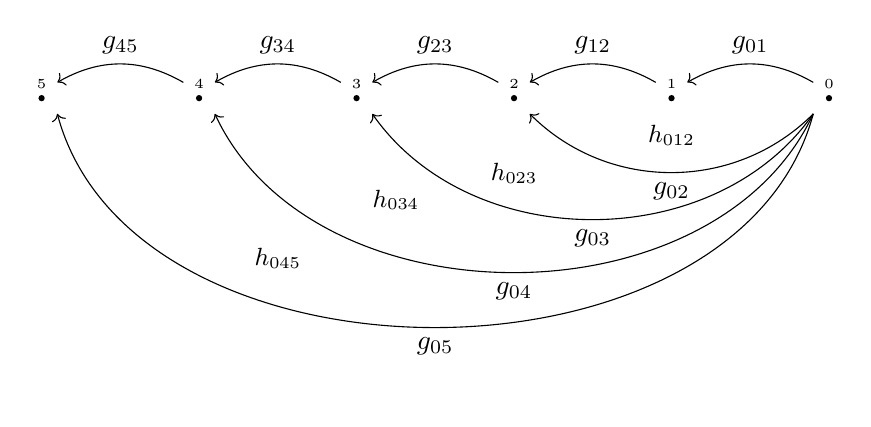
\begin{tikzpicture}[scale=2] 
       \coordinate (0) at (0,0); 
 	\coordinate (1) at (-1,0); 
	 \coordinate (2) at (-2,0);
	 \coordinate (3) at (-3,0);
	  \coordinate (4) at (-4,0);
	  \coordinate (5) at (-5,0);
	 \draw (0) node[above] {\tiny0};
	 \draw (1) node[above] {\tiny1};
	 \draw (2) node[above] {\tiny 2};
	 \draw (3) node[above] {\tiny 3};
	 \draw (4) node[above] {\tiny 4};
	 \draw (5) node[above] {\tiny 5};
 \fill[black] (0) circle[radius=0.02];
      \fill[black] (1) circle[radius=0.02];
      \fill[black] (2) circle[radius=0.02];
       \fill[black] (3) circle[radius=0.02];
       \fill[black] (4) circle[radius=0.02];
       \fill[black] (5) circle[radius=0.02];
      \draw[<-] ($(1)+(0.1,0.1)$) to [out=30,in=150] node[midway] (g01) {} ($(0)+(-0.1,0.1)$)   ;
	      \node[above] at (g01) {$g_{01}$};
	\draw[<-] ($(2)+(0.1,0.1)$)to [out=30,in=150] node[midway] (g12) {} ($(1)+(-0.1,0.1)$)    ;
	      \node[above] at (g12) {$g_{12}$};  
	 \draw[<-] ($(3)+(0.1,0.1)$)to [out=30,in=150] node[midway] (g23) {} ($(2)+(-0.1,0.1)$)    ;
	      \node[above] at (g23) {$g_{23}$};  
	   \draw[<-] ($(4)+(0.1,0.1)$)to [out=30,in=150] node[midway] (g34) {} ($(3)+(-0.1,0.1)$)    ;
	      \node[above] at (g34) {$g_{34}$};                          
	\draw[<-] ($(5)+(0.1,0.1)$)to [out=30,in=150] node[midway] (g45) {} ($(4)+(-0.1,0.1)$)    ;
	      \node[above] at (g45) {$g_{45}$};
	      
	\draw[<-] ($(2)+(0.1,-0.1)$)to [out=-45,in=-135] node[midway] (g02) {} ($(0)+(-0.1,-0.1)$)    ;
	      \node[below] at (g02) {$g_{02}$};  
	  \draw[<-] ($(3)+(0.1,-0.1)$)to [out=-55,in=-125] node[midway] (g03) {} ($(0)+(-0.1,-0.1)$)    ;
	      \node[below] at (g03) {$g_{03}$};     
	 \draw[<-] ($(4)+(0.1,-0.1)$)to [out=-65,in=-115] node[midway] (g04) {} ($(0)+(-0.1,-0.1)$)    ;
	      \node[below] at (g04) {$g_{04}$};     
	      
	 \draw[<-] ($(5)+(0.1,-0.1)$)to [out=-75,in=-105] node[midway] (g05) {} ($(0)+(-0.1,-0.1)$)    ;
	      \node[below] at (g05) {$g_{05}$};          	      
	 %\draw [line width=1pt, double distance=3pt, arrows = {-Latex[length=0pt 3 0]}]
        %($(1)-(0,-0.1)$) -- ($(g02) + (0, 0.1)$);    
        \draw ($(1)!0.5!(g02)$) node[] {\small $h_{012}$};   
        \draw ($(g03)!0.5!(g23)-(0,0.2)$) node[] {\small $h_{023}$}; 
        \draw ($(g04)!0.5!(g34)-(0,0.2)$) node[] {\small $h_{034}$};       
        \draw ($(g05)!0.5!(g45)-(0,0.4)$) node[] {\small $h_{045}$};   
\end{tikzpicture} \\ \hline

$a_2 = a'_2$ 
& 

 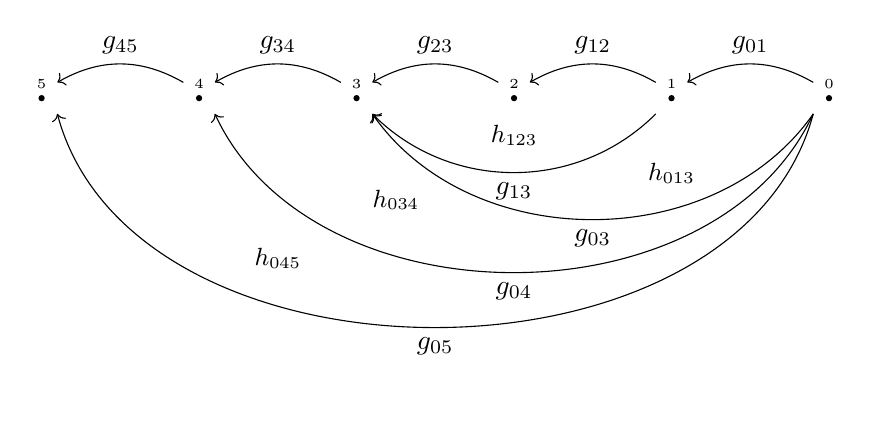
\begin{tikzpicture}[scale=2] 
       \coordinate (0) at (0,0); 
 	\coordinate (1) at (-1,0); 
	 \coordinate (2) at (-2,0);
	 \coordinate (3) at (-3,0);
	  \coordinate (4) at (-4,0);
	  \coordinate (5) at (-5,0);
	 \draw (0) node[above] {\tiny0};
	 \draw (1) node[above] {\tiny1};
	 \draw (2) node[above] {\tiny 2};
	 \draw (3) node[above] {\tiny 3};
	 \draw (4) node[above] {\tiny 4};
	 \draw (5) node[above] {\tiny 5};
 \fill[black] (0) circle[radius=0.02];
      \fill[black] (1) circle[radius=0.02];
      \fill[black] (2) circle[radius=0.02];
       \fill[black] (3) circle[radius=0.02];
       \fill[black] (4) circle[radius=0.02];
       \fill[black] (5) circle[radius=0.02];
      \draw[<-] ($(1)+(0.1,0.1)$) to [out=30,in=150] node[midway] (g01) {} ($(0)+(-0.1,0.1)$)   ;
	      \node[above] at (g01) {$g_{01}$};
	\draw[<-] ($(2)+(0.1,0.1)$)to [out=30,in=150] node[midway] (g12) {} ($(1)+(-0.1,0.1)$)    ;
	      \node[above] at (g12) {$g_{12}$};  
	 \draw[<-] ($(3)+(0.1,0.1)$)to [out=30,in=150] node[midway] (g23) {} ($(2)+(-0.1,0.1)$)    ;
	      \node[above] at (g23) {$g_{23}$};  
	   \draw[<-] ($(4)+(0.1,0.1)$)to [out=30,in=150] node[midway] (g34) {} ($(3)+(-0.1,0.1)$)    ;
	      \node[above] at (g34) {$g_{34}$};                          
	\draw[<-] ($(5)+(0.1,0.1)$)to [out=30,in=150] node[midway] (g45) {} ($(4)+(-0.1,0.1)$)    ;
	      \node[above] at (g45) {$g_{45}$};
	      
	\draw[<-] ($(3)+(0.1,-0.1)$)to [out=-45,in=-135] node[midway] (g13) {} ($(1)+(-0.1,-0.1)$)    ;
	      \node[below] at (g13) {$g_{13}$};  
	  \draw[<-] ($(3)+(0.1,-0.1)$)to [out=-55,in=-125] node[midway] (g03) {} ($(0)+(-0.1,-0.1)$)    ;
	      \node[below] at (g03) {$g_{03}$};     
	 \draw[<-] ($(4)+(0.1,-0.1)$)to [out=-65,in=-115] node[midway] (g04) {} ($(0)+(-0.1,-0.1)$)    ;
	      \node[below] at (g04) {$g_{04}$};     
	      
	 \draw[<-] ($(5)+(0.1,-0.1)$)to [out=-75,in=-105] node[midway] (g05) {} ($(0)+(-0.1,-0.1)$)    ;
	      \node[below] at (g05) {$g_{05}$};          	      
	 %\draw [line width=1pt, double distance=3pt, arrows = {-Latex[length=0pt 3 0]}]
        %($(1)-(0,-0.1)$) -- ($(g02) + (0, 0.1)$);    
        \draw ($(2)!0.5!(g13)$) node[] {\small $h_{123}$};   
        \draw ($(g03)!0.5!(g01)-(0,0.2)$) node[] {\small $h_{013}$}; 
        \draw ($(g04)!0.5!(g34)-(0,0.2)$) node[] {\small $h_{034}$};       
        \draw ($(g05)!0.5!(g45)-(0,0.4)$) node[] {\small $h_{045}$};   
\end{tikzpicture} \\ \hline
$a_3 = a'_3$ 
& 

 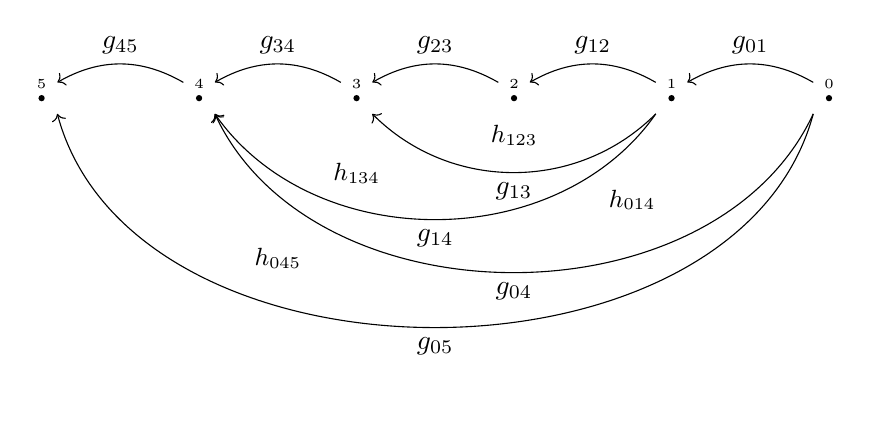
\begin{tikzpicture}[scale=2] 
       \coordinate (0) at (0,0); 
 	\coordinate (1) at (-1,0); 
	 \coordinate (2) at (-2,0);
	 \coordinate (3) at (-3,0);
	  \coordinate (4) at (-4,0);
	  \coordinate (5) at (-5,0);
	 \draw (0) node[above] {\tiny0};
	 \draw (1) node[above] {\tiny1};
	 \draw (2) node[above] {\tiny 2};
	 \draw (3) node[above] {\tiny 3};
	 \draw (4) node[above] {\tiny 4};
	 \draw (5) node[above] {\tiny 5};
 \fill[black] (0) circle[radius=0.02];
      \fill[black] (1) circle[radius=0.02];
      \fill[black] (2) circle[radius=0.02];
       \fill[black] (3) circle[radius=0.02];
       \fill[black] (4) circle[radius=0.02];
       \fill[black] (5) circle[radius=0.02];
      \draw[<-] ($(1)+(0.1,0.1)$) to [out=30,in=150] node[midway] (g01) {} ($(0)+(-0.1,0.1)$)   ;
	      \node[above] at (g01) {$g_{01}$};
	\draw[<-] ($(2)+(0.1,0.1)$)to [out=30,in=150] node[midway] (g12) {} ($(1)+(-0.1,0.1)$)    ;
	      \node[above] at (g12) {$g_{12}$};  
	 \draw[<-] ($(3)+(0.1,0.1)$)to [out=30,in=150] node[midway] (g23) {} ($(2)+(-0.1,0.1)$)    ;
	      \node[above] at (g23) {$g_{23}$};  
	   \draw[<-] ($(4)+(0.1,0.1)$)to [out=30,in=150] node[midway] (g34) {} ($(3)+(-0.1,0.1)$)    ;
	      \node[above] at (g34) {$g_{34}$};                          
	\draw[<-] ($(5)+(0.1,0.1)$)to [out=30,in=150] node[midway] (g45) {} ($(4)+(-0.1,0.1)$)    ;
	      \node[above] at (g45) {$g_{45}$};
	      
	\draw[<-] ($(3)+(0.1,-0.1)$)to [out=-45,in=-135] node[midway] (g13) {} ($(1)+(-0.1,-0.1)$)    ;
	      \node[below] at (g13) {$g_{13}$};  
	  \draw[<-] ($(4)+(0.1,-0.1)$)to [out=-55,in=-125] node[midway] (g14) {} ($(1)+(-0.1,-0.1)$)    ;
	      \node[below] at (g14) {$g_{14}$};     
	 \draw[<-] ($(4)+(0.1,-0.1)$)to [out=-65,in=-115] node[midway] (g04) {} ($(0)+(-0.1,-0.1)$)    ;
	      \node[below] at (g04) {$g_{04}$};     
	      
	 \draw[<-] ($(5)+(0.1,-0.1)$)to [out=-75,in=-105] node[midway] (g05) {} ($(0)+(-0.1,-0.1)$)    ;
	      \node[below] at (g05) {$g_{05}$};          	      
	 %\draw [line width=1pt, double distance=3pt, arrows = {-Latex[length=0pt 3 0]}]
        %($(1)-(0,-0.1)$) -- ($(g02) + (0, 0.1)$);    
        \draw ($(2)!0.5!(g13)$) node[] {\small $h_{123}$};   
        \draw ($(g14)!0.5!(g34)-(0,0.2)$) node[] {\small $h_{134}$}; 
        \draw ($(g04)!0.5!(g01)-(0,0.2)$) node[] {\small $h_{014}$};       
        \draw ($(g05)!0.5!(g45)-(0,0.4)$) node[] {\small $h_{045}$};   
\end{tikzpicture} \\ \hline
$a_4 = a'_4$ 
& 

 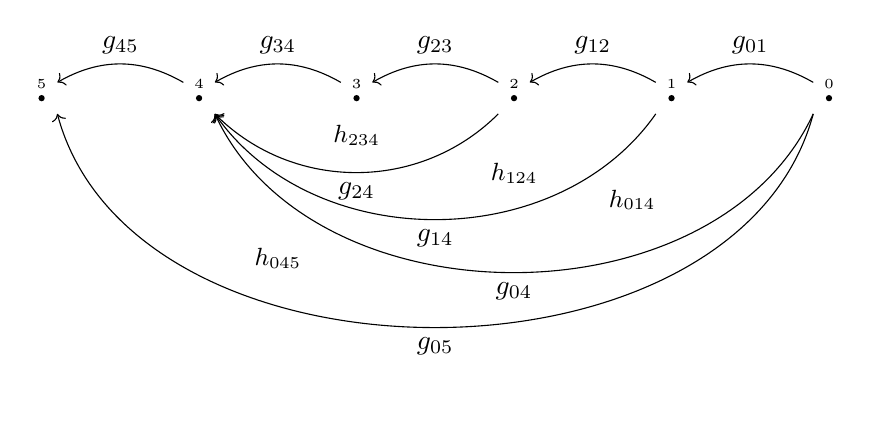
\begin{tikzpicture}[scale=2] 
       \coordinate (0) at (0,0); 
 	\coordinate (1) at (-1,0); 
	 \coordinate (2) at (-2,0);
	 \coordinate (3) at (-3,0);
	  \coordinate (4) at (-4,0);
	  \coordinate (5) at (-5,0);
	 \draw (0) node[above] {\tiny0};
	 \draw (1) node[above] {\tiny1};
	 \draw (2) node[above] {\tiny 2};
	 \draw (3) node[above] {\tiny 3};
	 \draw (4) node[above] {\tiny 4};
	 \draw (5) node[above] {\tiny 5};
 \fill[black] (0) circle[radius=0.02];
      \fill[black] (1) circle[radius=0.02];
      \fill[black] (2) circle[radius=0.02];
       \fill[black] (3) circle[radius=0.02];
       \fill[black] (4) circle[radius=0.02];
       \fill[black] (5) circle[radius=0.02];
      \draw[<-] ($(1)+(0.1,0.1)$) to [out=30,in=150] node[midway] (g01) {} ($(0)+(-0.1,0.1)$)   ;
	      \node[above] at (g01) {$g_{01}$};
	\draw[<-] ($(2)+(0.1,0.1)$)to [out=30,in=150] node[midway] (g12) {} ($(1)+(-0.1,0.1)$)    ;
	      \node[above] at (g12) {$g_{12}$};  
	 \draw[<-] ($(3)+(0.1,0.1)$)to [out=30,in=150] node[midway] (g23) {} ($(2)+(-0.1,0.1)$)    ;
	      \node[above] at (g23) {$g_{23}$};  
	   \draw[<-] ($(4)+(0.1,0.1)$)to [out=30,in=150] node[midway] (g34) {} ($(3)+(-0.1,0.1)$)    ;
	      \node[above] at (g34) {$g_{34}$};                          
	\draw[<-] ($(5)+(0.1,0.1)$)to [out=30,in=150] node[midway] (g45) {} ($(4)+(-0.1,0.1)$)    ;
	      \node[above] at (g45) {$g_{45}$};
	      
	\draw[<-] ($(4)+(0.1,-0.1)$)to [out=-45,in=-135] node[midway] (g24) {} ($(2)+(-0.1,-0.1)$)    ;
	      \node[below] at (g24) {$g_{24}$};  
	  \draw[<-] ($(4)+(0.1,-0.1)$)to [out=-55,in=-125] node[midway] (g14) {} ($(1)+(-0.1,-0.1)$)    ;
	      \node[below] at (g14) {$g_{14}$};     
	 \draw[<-] ($(4)+(0.1,-0.1)$)to [out=-65,in=-115] node[midway] (g04) {} ($(0)+(-0.1,-0.1)$)    ;
	      \node[below] at (g04) {$g_{04}$};     
	      
	 \draw[<-] ($(5)+(0.1,-0.1)$)to [out=-75,in=-105] node[midway] (g05) {} ($(0)+(-0.1,-0.1)$)    ;
	      \node[below] at (g05) {$g_{05}$};          	      
	 %\draw [line width=1pt, double distance=3pt, arrows = {-Latex[length=0pt 3 0]}]
        %($(1)-(0,-0.1)$) -- ($(g02) + (0, 0.1)$);    
        \draw ($(3)!0.5!(g24)$) node[] {\small $h_{234}$};   
        \draw ($(g14)!0.5!(g12)-(0,0.2)$) node[] {\small $h_{124}$}; 
        \draw ($(g04)!0.5!(g01)-(0,0.2)$) node[] {\small $h_{014}$};       
        \draw ($(g05)!0.5!(g45)-(0,0.4)$) node[] {\small $h_{045}$};   
\end{tikzpicture} \\ \hline
$a_5 = a'_5$ 
& 

 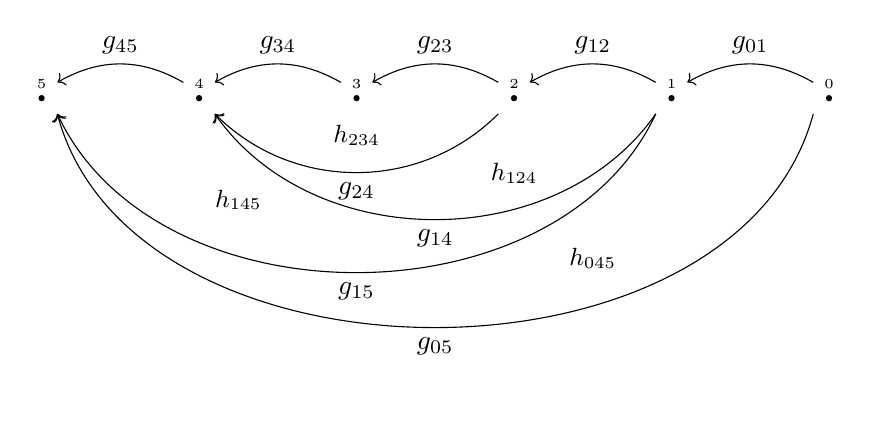
\begin{tikzpicture}[scale=2] 
       \coordinate (0) at (0,0); 
 	\coordinate (1) at (-1,0); 
	 \coordinate (2) at (-2,0);
	 \coordinate (3) at (-3,0);
	  \coordinate (4) at (-4,0);
	  \coordinate (5) at (-5,0);
	 \draw (0) node[above] {\tiny0};
	 \draw (1) node[above] {\tiny1};
	 \draw (2) node[above] {\tiny 2};
	 \draw (3) node[above] {\tiny 3};
	 \draw (4) node[above] {\tiny 4};
	 \draw (5) node[above] {\tiny 5};
 \fill[black] (0) circle[radius=0.02];
      \fill[black] (1) circle[radius=0.02];
      \fill[black] (2) circle[radius=0.02];
       \fill[black] (3) circle[radius=0.02];
       \fill[black] (4) circle[radius=0.02];
       \fill[black] (5) circle[radius=0.02];
      \draw[<-] ($(1)+(0.1,0.1)$) to [out=30,in=150] node[midway] (g01) {} ($(0)+(-0.1,0.1)$)   ;
	      \node[above] at (g01) {$g_{01}$};
	\draw[<-] ($(2)+(0.1,0.1)$)to [out=30,in=150] node[midway] (g12) {} ($(1)+(-0.1,0.1)$)    ;
	      \node[above] at (g12) {$g_{12}$};  
	 \draw[<-] ($(3)+(0.1,0.1)$)to [out=30,in=150] node[midway] (g23) {} ($(2)+(-0.1,0.1)$)    ;
	      \node[above] at (g23) {$g_{23}$};  
	   \draw[<-] ($(4)+(0.1,0.1)$)to [out=30,in=150] node[midway] (g34) {} ($(3)+(-0.1,0.1)$)    ;
	      \node[above] at (g34) {$g_{34}$};                          
	\draw[<-] ($(5)+(0.1,0.1)$)to [out=30,in=150] node[midway] (g45) {} ($(4)+(-0.1,0.1)$)    ;
	      \node[above] at (g45) {$g_{45}$};
	      
	\draw[<-] ($(4)+(0.1,-0.1)$)to [out=-45,in=-135] node[midway] (g24) {} ($(2)+(-0.1,-0.1)$)    ;
	      \node[below] at (g24) {$g_{24}$};  
	  \draw[<-] ($(4)+(0.1,-0.1)$)to [out=-55,in=-125] node[midway] (g14) {} ($(1)+(-0.1,-0.1)$)    ;
	      \node[below] at (g14) {$g_{14}$};     
	 \draw[<-] ($(5)+(0.1,-0.1)$)to [out=-65,in=-115] node[midway] (g15) {} ($(1)+(-0.1,-0.1)$)    ;
	      \node[below] at (g15) {$g_{15}$};     
	      
	 \draw[<-] ($(5)+(0.1,-0.1)$)to [out=-75,in=-105] node[midway] (g05) {} ($(0)+(-0.1,-0.1)$)    ;
	      \node[below] at (g05) {$g_{05}$};          	      
	 %\draw [line width=1pt, double distance=3pt, arrows = {-Latex[length=0pt 3 0]}]
        %($(1)-(0,-0.1)$) -- ($(g02) + (0, 0.1)$);    
        \draw ($(3)!0.5!(g24)$) node[] {\small $h_{234}$};   
        \draw ($(g14)!0.5!(g12)-(0,0.2)$) node[] {\small $h_{124}$}; 
        \draw ($(g15)!0.5!(g45)-(0,0.2)$) node[] {\small $h_{145}$};       
        \draw ($(g05)!0.5!(g01)-(0,0.4)$) node[] {\small $h_{045}$};   
\end{tikzpicture} \\ \hline
$a_6 = a'_6$ 
& 

 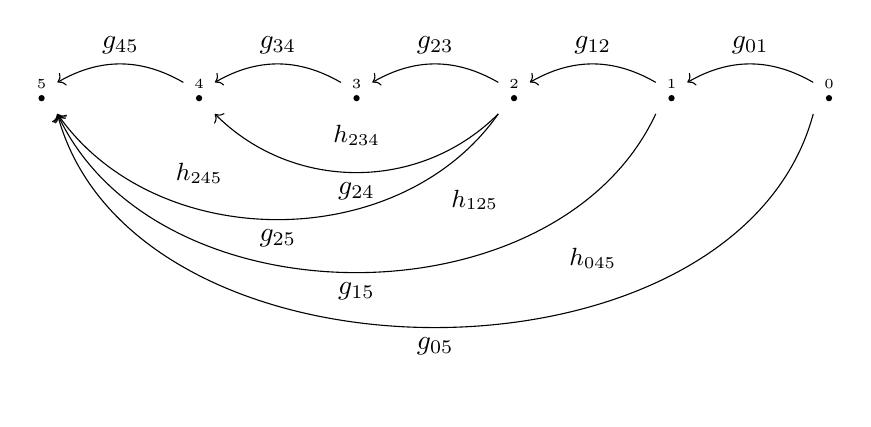
\begin{tikzpicture}[scale=2] 
       \coordinate (0) at (0,0); 
 	\coordinate (1) at (-1,0); 
	 \coordinate (2) at (-2,0);
	 \coordinate (3) at (-3,0);
	  \coordinate (4) at (-4,0);
	  \coordinate (5) at (-5,0);
	 \draw (0) node[above] {\tiny0};
	 \draw (1) node[above] {\tiny1};
	 \draw (2) node[above] {\tiny 2};
	 \draw (3) node[above] {\tiny 3};
	 \draw (4) node[above] {\tiny 4};
	 \draw (5) node[above] {\tiny 5};
 \fill[black] (0) circle[radius=0.02];
      \fill[black] (1) circle[radius=0.02];
      \fill[black] (2) circle[radius=0.02];
       \fill[black] (3) circle[radius=0.02];
       \fill[black] (4) circle[radius=0.02];
       \fill[black] (5) circle[radius=0.02];
      \draw[<-] ($(1)+(0.1,0.1)$) to [out=30,in=150] node[midway] (g01) {} ($(0)+(-0.1,0.1)$)   ;
	      \node[above] at (g01) {$g_{01}$};
	\draw[<-] ($(2)+(0.1,0.1)$)to [out=30,in=150] node[midway] (g12) {} ($(1)+(-0.1,0.1)$)    ;
	      \node[above] at (g12) {$g_{12}$};  
	 \draw[<-] ($(3)+(0.1,0.1)$)to [out=30,in=150] node[midway] (g23) {} ($(2)+(-0.1,0.1)$)    ;
	      \node[above] at (g23) {$g_{23}$};  
	   \draw[<-] ($(4)+(0.1,0.1)$)to [out=30,in=150] node[midway] (g34) {} ($(3)+(-0.1,0.1)$)    ;
	      \node[above] at (g34) {$g_{34}$};                          
	\draw[<-] ($(5)+(0.1,0.1)$)to [out=30,in=150] node[midway] (g45) {} ($(4)+(-0.1,0.1)$)    ;
	      \node[above] at (g45) {$g_{45}$};
	      
	\draw[<-] ($(4)+(0.1,-0.1)$)to [out=-45,in=-135] node[midway] (g24) {} ($(2)+(-0.1,-0.1)$)    ;
	      \node[below] at (g24) {$g_{24}$};  
	  \draw[<-] ($(5)+(0.1,-0.1)$)to [out=-55,in=-125] node[midway] (g25) {} ($(2)+(-0.1,-0.1)$)    ;
	      \node[below] at (g25) {$g_{25}$};     
	 \draw[<-] ($(5)+(0.1,-0.1)$)to [out=-65,in=-115] node[midway] (g15) {} ($(1)+(-0.1,-0.1)$)    ;
	      \node[below] at (g15) {$g_{15}$};     
	      
	 \draw[<-] ($(5)+(0.1,-0.1)$)to [out=-75,in=-105] node[midway] (g05) {} ($(0)+(-0.1,-0.1)$)    ;
	      \node[below] at (g05) {$g_{05}$};          	      
	 %\draw [line width=1pt, double distance=3pt, arrows = {-Latex[length=0pt 3 0]}]
        %($(1)-(0,-0.1)$) -- ($(g02) + (0, 0.1)$);    
        \draw ($(3)!0.5!(g24)$) node[] {\small $h_{234}$};   
        \draw ($(g25)!0.5!(g45)-(0,0.2)$) node[] {\small $h_{245}$}; 
        \draw ($(g15)!0.5!(g12)-(0,0.2)$) node[] {\small $h_{125}$};       
        \draw ($(g05)!0.5!(g01)-(0,0.4)$) node[] {\small $h_{045}$};   
\end{tikzpicture} \\ \hline
$a_7 = a'_7$ 
& 

 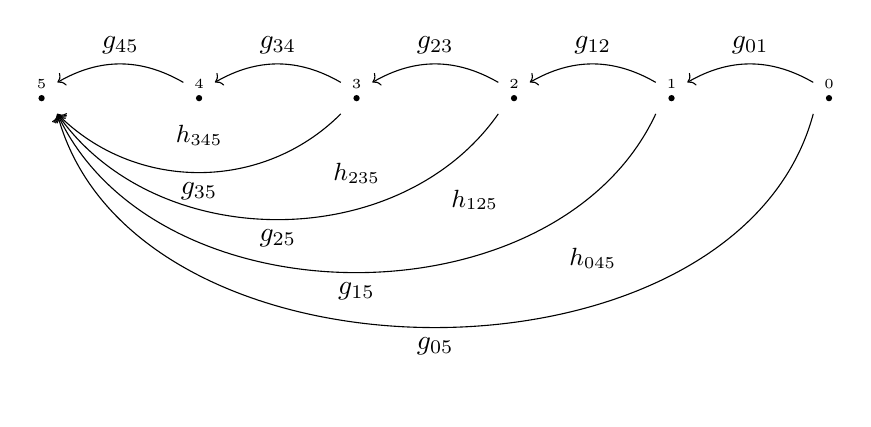
\begin{tikzpicture}[scale=2] 
       \coordinate (0) at (0,0); 
 	\coordinate (1) at (-1,0); 
	 \coordinate (2) at (-2,0);
	 \coordinate (3) at (-3,0);
	  \coordinate (4) at (-4,0);
	  \coordinate (5) at (-5,0);
	 \draw (0) node[above] {\tiny0};
	 \draw (1) node[above] {\tiny1};
	 \draw (2) node[above] {\tiny 2};
	 \draw (3) node[above] {\tiny 3};
	 \draw (4) node[above] {\tiny 4};
	 \draw (5) node[above] {\tiny 5};
 \fill[black] (0) circle[radius=0.02];
      \fill[black] (1) circle[radius=0.02];
      \fill[black] (2) circle[radius=0.02];
       \fill[black] (3) circle[radius=0.02];
       \fill[black] (4) circle[radius=0.02];
       \fill[black] (5) circle[radius=0.02];
      \draw[<-] ($(1)+(0.1,0.1)$) to [out=30,in=150] node[midway] (g01) {} ($(0)+(-0.1,0.1)$)   ;
	      \node[above] at (g01) {$g_{01}$};
	\draw[<-] ($(2)+(0.1,0.1)$)to [out=30,in=150] node[midway] (g12) {} ($(1)+(-0.1,0.1)$)    ;
	      \node[above] at (g12) {$g_{12}$};  
	 \draw[<-] ($(3)+(0.1,0.1)$)to [out=30,in=150] node[midway] (g23) {} ($(2)+(-0.1,0.1)$)    ;
	      \node[above] at (g23) {$g_{23}$};  
	   \draw[<-] ($(4)+(0.1,0.1)$)to [out=30,in=150] node[midway] (g34) {} ($(3)+(-0.1,0.1)$)    ;
	      \node[above] at (g34) {$g_{34}$};                          
	\draw[<-] ($(5)+(0.1,0.1)$)to [out=30,in=150] node[midway] (g45) {} ($(4)+(-0.1,0.1)$)    ;
	      \node[above] at (g45) {$g_{45}$};
	      
	\draw[<-] ($(5)+(0.1,-0.1)$)to [out=-45,in=-135] node[midway] (g35) {} ($(3)+(-0.1,-0.1)$)    ;
	      \node[below] at (g35) {$g_{35}$};  
	  \draw[<-] ($(5)+(0.1,-0.1)$)to [out=-55,in=-125] node[midway] (g25) {} ($(2)+(-0.1,-0.1)$)    ;
	      \node[below] at (g25) {$g_{25}$};     
	 \draw[<-] ($(5)+(0.1,-0.1)$)to [out=-65,in=-115] node[midway] (g15) {} ($(1)+(-0.1,-0.1)$)    ;
	      \node[below] at (g15) {$g_{15}$};     
	      
	 \draw[<-] ($(5)+(0.1,-0.1)$)to [out=-75,in=-105] node[midway] (g05) {} ($(0)+(-0.1,-0.1)$)    ;
	      \node[below] at (g05) {$g_{05}$};          	      
	 %\draw [line width=1pt, double distance=3pt, arrows = {-Latex[length=0pt 3 0]}]
        %($(1)-(0,-0.1)$) -- ($(g02) + (0, 0.1)$);    
        \draw ($(4)!0.5!(g35)$) node[] {\small $h_{345}$};   
        \draw ($(g25)!0.5!(g23)-(0,0.2)$) node[] {\small $h_{235}$}; 
        \draw ($(g15)!0.5!(g12)-(0,0.2)$) node[] {\small $h_{125}$};       
        \draw ($(g05)!0.5!(g01)-(0,0.4)$) node[] {\small $h_{045}$};   
\end{tikzpicture} \\ \hline
$a_9$ 
& 

 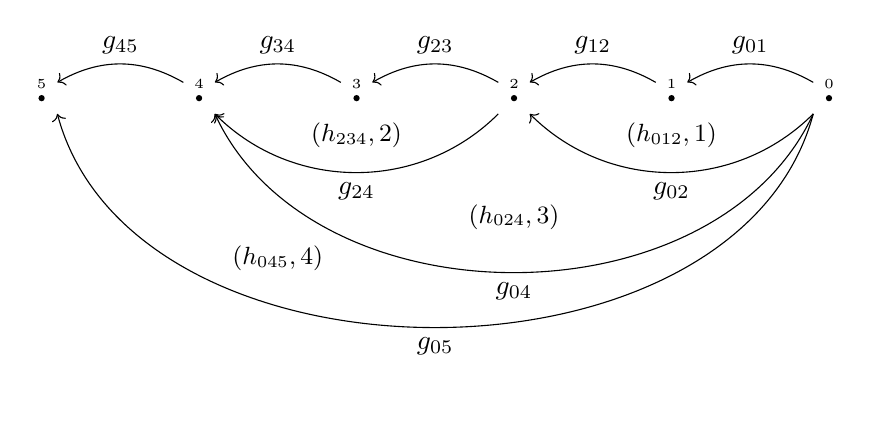
\begin{tikzpicture}[scale=2] 
       \coordinate (0) at (0,0); 
 	\coordinate (1) at (-1,0); 
	 \coordinate (2) at (-2,0);
	 \coordinate (3) at (-3,0);
	  \coordinate (4) at (-4,0);
	  \coordinate (5) at (-5,0);
	 \draw (0) node[above] {\tiny0};
	 \draw (1) node[above] {\tiny1};
	 \draw (2) node[above] {\tiny 2};
	 \draw (3) node[above] {\tiny 3};
	 \draw (4) node[above] {\tiny 4};
	 \draw (5) node[above] {\tiny 5};
 \fill[black] (0) circle[radius=0.02];
      \fill[black] (1) circle[radius=0.02];
      \fill[black] (2) circle[radius=0.02];
       \fill[black] (3) circle[radius=0.02];
       \fill[black] (4) circle[radius=0.02];
       \fill[black] (5) circle[radius=0.02];
      \draw[<-] ($(1)+(0.1,0.1)$) to [out=30,in=150] node[midway] (g01) {} ($(0)+(-0.1,0.1)$)   ;
	      \node[above] at (g01) {$g_{01}$};
	\draw[<-] ($(2)+(0.1,0.1)$)to [out=30,in=150] node[midway] (g12) {} ($(1)+(-0.1,0.1)$)    ;
	      \node[above] at (g12) {$g_{12}$};  
	 \draw[<-] ($(3)+(0.1,0.1)$)to [out=30,in=150] node[midway] (g23) {} ($(2)+(-0.1,0.1)$)    ;
	      \node[above] at (g23) {$g_{23}$};  
	   \draw[<-] ($(4)+(0.1,0.1)$)to [out=30,in=150] node[midway] (g34) {} ($(3)+(-0.1,0.1)$)    ;
	      \node[above] at (g34) {$g_{34}$};                          
	\draw[<-] ($(5)+(0.1,0.1)$)to [out=30,in=150] node[midway] (g45) {} ($(4)+(-0.1,0.1)$)    ;
	      \node[above] at (g45) {$g_{45}$};
	      
	\draw[<-] ($(2)+(0.1,-0.1)$)to [out=-45,in=-135] node[midway] (g02) {} ($(0)+(-0.1,-0.1)$)    ;
	      \node[below] at (g02) {$g_{02}$};  
	  \draw[<-] ($(4)+(0.1,-0.1)$)to [out=-45,in=-135] node[midway] (g24) {} ($(2)+(-0.1,-0.1)$)    ;
	      \node[below] at (g24) {$g_{24}$};     
	 \draw[<-] ($(4)+(0.1,-0.1)$)to [out=-65,in=-115] node[midway] (g04) {} ($(0)+(-0.1,-0.1)$)    ;
	      \node[below] at (g04) {$g_{04}$};     
	      
	 \draw[<-] ($(5)+(0.1,-0.1)$)to [out=-75,in=-105] node[midway] (g05) {} ($(0)+(-0.1,-0.1)$)    ;
	      \node[below] at (g05) {$g_{05}$};          	      
	 %\draw [line width=1pt, double distance=3pt, arrows = {-Latex[length=0pt 3 0]}]
        %($(1)-(0,-0.1)$) -- ($(g02) + (0, 0.1)$);    
        \draw ($(1)!0.5!(g02)$) node[] {\small $(h_{012},1)$};   
        \draw ($(3)!0.5!(g24)-(0,0)$) node[] {\small $(h_{234},2)$}; 
        \draw ($(g04)!0.5!(2)-(0,0.2)$) node[] {\small $(h_{024},3)$};       
        \draw ($(g05)!0.5!(g45)-(0,0.4)$) node[] {\small $(h_{045},4)$};   
\end{tikzpicture} \\ \hline
$a_8 = a'_{20}$ 
& 

 \begin{tikzpicture}[scale=2] 
       \coordinate (0) at (0,0); 
 	\coordinate (1) at (-1,0); 
	 \coordinate (2) at (-2,0);
	 \coordinate (3) at (-3,0);
	  \coordinate (4) at (-4,0);
	  \coordinate (5) at (-5,0);
	 \draw (0) node[above] {\tiny0};
	 \draw (1) node[above] {\tiny1};
	 \draw (2) node[above] {\tiny 2};
	 \draw (3) node[above] {\tiny 3};
	 \draw (4) node[above] {\tiny 4};
	 \draw (5) node[above] {\tiny 5};
 \fill[black] (0) circle[radius=0.02];
      \fill[black] (1) circle[radius=0.02];
      \fill[black] (2) circle[radius=0.02];
       \fill[black] (3) circle[radius=0.02];
       \fill[black] (4) circle[radius=0.02];
       \fill[black] (5) circle[radius=0.02];
      \draw[<-] ($(1)+(0.1,0.1)$) to [out=30,in=150] node[midway] (g01) {} ($(0)+(-0.1,0.1)$)   ;
	      \node[above] at (g01) {$g_{01}$};
	\draw[<-] ($(2)+(0.1,0.1)$)to [out=30,in=150] node[midway] (g12) {} ($(1)+(-0.1,0.1)$)    ;
	      \node[above] at (g12) {$g_{12}$};  
	 \draw[<-] ($(3)+(0.1,0.1)$)to [out=30,in=150] node[midway] (g23) {} ($(2)+(-0.1,0.1)$)    ;
	      \node[above] at (g23) {$g_{23}$};  
	   \draw[<-] ($(4)+(0.1,0.1)$)to [out=30,in=150] node[midway] (g34) {} ($(3)+(-0.1,0.1)$)    ;
	      \node[above] at (g34) {$g_{34}$};                          
	\draw[<-] ($(5)+(0.1,0.1)$)to [out=30,in=150] node[midway] (g45) {} ($(4)+(-0.1,0.1)$)    ;
	      \node[above] at (g45) {$g_{45}$};
	      
	\draw[<-] ($(2)+(0.1,-0.1)$)to [out=-45,in=-135] node[midway] (g02) {} ($(0)+(-0.1,-0.1)$)    ;
	      \node[below] at (g02) {$g_{02}$};  
	  \draw[<-] ($(4)+(0.1,-0.1)$)to [out=-45,in=-135] node[midway] (g24) {} ($(2)+(-0.1,-0.1)$)    ;
	      \node[below] at (g24) {$g_{24}$};     
	 \draw[<-] ($(4)+(0.1,-0.1)$)to [out=-65,in=-115] node[midway] (g04) {} ($(0)+(-0.1,-0.1)$)    ;
	      \node[below] at (g04) {$g_{04}$};     
	      
	 \draw[<-] ($(5)+(0.1,-0.1)$)to [out=-75,in=-105] node[midway] (g05) {} ($(0)+(-0.1,-0.1)$)    ;
	      \node[below] at (g05) {$g_{05}$};          	      
	 %\draw [line width=1pt, double distance=3pt, arrows = {-Latex[length=0pt 3 0]}]
        %($(1)-(0,-0.1)$) -- ($(g02) + (0, 0.1)$);    
        \draw ($(1)!0.5!(g02)$) node[] {\small $(h_{012},2)$};   
        \draw ($(3)!0.5!(g24)-(0,0)$) node[] {\small $(h_{234},1)$}; 
        \draw ($(g04)!0.5!(2)-(0,0.2)$) node[] {\small $(h_{024},3)$};       
        \draw ($(g05)!0.5!(g45)-(0,0.4)$) node[] {\small $(h_{045},4)$};   
\end{tikzpicture} \\ \hline
$a_{10} = a'_{21}$ 
& 

 \begin{tikzpicture}[scale=2] 
       \coordinate (0) at (0,0); 
 	\coordinate (1) at (-1,0); 
	 \coordinate (2) at (-2,0);
	 \coordinate (3) at (-3,0);
	  \coordinate (4) at (-4,0);
	  \coordinate (5) at (-5,0);
	 \draw (0) node[above] {\tiny0};
	 \draw (1) node[above] {\tiny1};
	 \draw (2) node[above] {\tiny 2};
	 \draw (3) node[above] {\tiny 3};
	 \draw (4) node[above] {\tiny 4};
	 \draw (5) node[above] {\tiny 5};
 \fill[black] (0) circle[radius=0.02];
      \fill[black] (1) circle[radius=0.02];
      \fill[black] (2) circle[radius=0.02];
       \fill[black] (3) circle[radius=0.02];
       \fill[black] (4) circle[radius=0.02];
       \fill[black] (5) circle[radius=0.02];
      \draw[<-] ($(1)+(0.1,0.1)$) to [out=30,in=150] node[midway] (g01) {} ($(0)+(-0.1,0.1)$)   ;
	      \node[above] at (g01) {$g_{01}$};
	\draw[<-] ($(2)+(0.1,0.1)$)to [out=30,in=150] node[midway] (g12) {} ($(1)+(-0.1,0.1)$)    ;
	      \node[above] at (g12) {$g_{12}$};  
	 \draw[<-] ($(3)+(0.1,0.1)$)to [out=30,in=150] node[midway] (g23) {} ($(2)+(-0.1,0.1)$)    ;
	      \node[above] at (g23) {$g_{23}$};  
	   \draw[<-] ($(4)+(0.1,0.1)$)to [out=30,in=150] node[midway] (g34) {} ($(3)+(-0.1,0.1)$)    ;
	      \node[above] at (g34) {$g_{34}$};                          
	\draw[<-] ($(5)+(0.1,0.1)$)to [out=30,in=150] node[midway] (g45) {} ($(4)+(-0.1,0.1)$)    ;
	      \node[above] at (g45) {$g_{45}$};
	      
	\draw[<-] ($(2)+(0.1,-0.1)$)to [out=-45,in=-135] node[midway] (g02) {} ($(0)+(-0.1,-0.1)$)    ;
	      \node[below] at (g02) {$g_{02}$};  
	  \draw[<-] ($(4)+(0.1,-0.1)$)to [out=-45,in=-135] node[midway] (g24) {} ($(2)+(-0.1,-0.1)$)    ;
	      \node[below] at (g24) {$g_{24}$};     
	 \draw[<-] ($(5)+(0.1,-0.1)$)to [out=-65,in=-115] node[midway] (g25) {} ($(2)+(-0.1,-0.1)$)    ;
	      \node[below] at (g25) {$g_{25}$};     
	      
	 \draw[<-] ($(5)+(0.1,-0.1)$)to [out=-75,in=-105] node[midway] (g05) {} ($(0)+(-0.1,-0.1)$)    ;
	      \node[below] at (g05) {$g_{05}$};          	      
	 %\draw [line width=1pt, double distance=3pt, arrows = {-Latex[length=0pt 3 0]}]
        %($(1)-(0,-0.1)$) -- ($(g02) + (0, 0.1)$);    
        \draw ($(1)!0.5!(g02)$) node[] {\small $(h_{012},1)$};   
        \draw ($(3)!0.5!(g24)-(0,0)$) node[] {\small $(h_{234},2)$}; 
        \draw ($(g25)!0.5!(g45)-(0,0.2)$) node[] {\small $(h_{245},3)$};       
        \draw ($(g05)!0.5!(g02)-(0,0)$) node[] {\small $(h_{025},4)$};   
\end{tikzpicture} \\ \hline
$a_{11} $ 
& 

 \begin{tikzpicture}[scale=2] 
       \coordinate (0) at (0,0); 
 	\coordinate (1) at (-1,0); 
	 \coordinate (2) at (-2,0);
	 \coordinate (3) at (-3,0);
	  \coordinate (4) at (-4,0);
	  \coordinate (5) at (-5,0);
	 \draw (0) node[above] {\tiny0};
	 \draw (1) node[above] {\tiny1};
	 \draw (2) node[above] {\tiny 2};
	 \draw (3) node[above] {\tiny 3};
	 \draw (4) node[above] {\tiny 4};
	 \draw (5) node[above] {\tiny 5};
 \fill[black] (0) circle[radius=0.02];
      \fill[black] (1) circle[radius=0.02];
      \fill[black] (2) circle[radius=0.02];
       \fill[black] (3) circle[radius=0.02];
       \fill[black] (4) circle[radius=0.02];
       \fill[black] (5) circle[radius=0.02];
      \draw[<-] ($(1)+(0.1,0.1)$) to [out=30,in=150] node[midway] (g01) {} ($(0)+(-0.1,0.1)$)   ;
	      \node[above] at (g01) {$g_{01}$};
	\draw[<-] ($(2)+(0.1,0.1)$)to [out=30,in=150] node[midway] (g12) {} ($(1)+(-0.1,0.1)$)    ;
	      \node[above] at (g12) {$g_{12}$};  
	 \draw[<-] ($(3)+(0.1,0.1)$)to [out=30,in=150] node[midway] (g23) {} ($(2)+(-0.1,0.1)$)    ;
	      \node[above] at (g23) {$g_{23}$};  
	   \draw[<-] ($(4)+(0.1,0.1)$)to [out=30,in=150] node[midway] (g34) {} ($(3)+(-0.1,0.1)$)    ;
	      \node[above] at (g34) {$g_{34}$};                          
	\draw[<-] ($(5)+(0.1,0.1)$)to [out=30,in=150] node[midway] (g45) {} ($(4)+(-0.1,0.1)$)    ;
	      \node[above] at (g45) {$g_{45}$};
	      
	\draw[<-] ($(2)+(0.1,-0.1)$)to [out=-45,in=-135] node[midway] (g02) {} ($(0)+(-0.1,-0.1)$)    ;
	      \node[below] at (g02) {$g_{02}$};  
	  \draw[<-] ($(4)+(0.1,-0.1)$)to [out=-45,in=-135] node[midway] (g24) {} ($(2)+(-0.1,-0.1)$)    ;
	      \node[below] at (g24) {$g_{24}$};     
	 \draw[<-] ($(5)+(0.1,-0.1)$)to [out=-65,in=-115] node[midway] (g25) {} ($(2)+(-0.1,-0.1)$)    ;
	      \node[below] at (g25) {$g_{25}$};     
	      
	 \draw[<-] ($(5)+(0.1,-0.1)$)to [out=-75,in=-105] node[midway] (g05) {} ($(0)+(-0.1,-0.1)$)    ;
	      \node[below] at (g05) {$g_{05}$};          	      
	 %\draw [line width=1pt, double distance=3pt, arrows = {-Latex[length=0pt 3 0]}]
        %($(1)-(0,-0.1)$) -- ($(g02) + (0, 0.1)$);    
        \draw ($(1)!0.5!(g02)$) node[] {\small $(h_{012},2)$};   
        \draw ($(3)!0.5!(g24)-(0,0)$) node[] {\small $(h_{234},1)$}; 
        \draw ($(g25)!0.5!(g45)-(0,0.2)$) node[] {\small $(h_{245},3)$};       
        \draw ($(g05)!0.5!(g02)-(0,0)$) node[] {\small $(h_{025},4)$};   
\end{tikzpicture} \\ \hline
$a_{12} = a'_{22}$ 
& 

 \begin{tikzpicture}[scale=2] 
       \coordinate (0) at (0,0); 
 	\coordinate (1) at (-1,0); 
	 \coordinate (2) at (-2,0);
	 \coordinate (3) at (-3,0);
	  \coordinate (4) at (-4,0);
	  \coordinate (5) at (-5,0);
	 \draw (0) node[above] {\tiny0};
	 \draw (1) node[above] {\tiny1};
	 \draw (2) node[above] {\tiny 2};
	 \draw (3) node[above] {\tiny 3};
	 \draw (4) node[above] {\tiny 4};
	 \draw (5) node[above] {\tiny 5};
 \fill[black] (0) circle[radius=0.02];
      \fill[black] (1) circle[radius=0.02];
      \fill[black] (2) circle[radius=0.02];
       \fill[black] (3) circle[radius=0.02];
       \fill[black] (4) circle[radius=0.02];
       \fill[black] (5) circle[radius=0.02];
      \draw[<-] ($(1)+(0.1,0.1)$) to [out=30,in=150] node[midway] (g01) {} ($(0)+(-0.1,0.1)$)   ;
	      \node[above] at (g01) {$g_{01}$};
	\draw[<-] ($(2)+(0.1,0.1)$)to [out=30,in=150] node[midway] (g12) {} ($(1)+(-0.1,0.1)$)    ;
	      \node[above] at (g12) {$g_{12}$};  
	 \draw[<-] ($(3)+(0.1,0.1)$)to [out=30,in=150] node[midway] (g23) {} ($(2)+(-0.1,0.1)$)    ;
	      \node[above] at (g23) {$g_{23}$};  
	   \draw[<-] ($(4)+(0.1,0.1)$)to [out=30,in=150] node[midway] (g34) {} ($(3)+(-0.1,0.1)$)    ;
	      \node[above] at (g34) {$g_{34}$};                          
	\draw[<-] ($(5)+(0.1,0.1)$)to [out=30,in=150] node[midway] (g45) {} ($(4)+(-0.1,0.1)$)    ;
	      \node[above] at (g45) {$g_{45}$};
	      
	\draw[<-] ($(2)+(0.1,-0.1)$)to [out=-45,in=-135] node[midway] (g02) {} ($(0)+(-0.1,-0.1)$)    ;
	      \node[below] at (g02) {$g_{02}$};  
	  \draw[<-] ($(4)+(0.1,-0.1)$)to [out=-45,in=-135] node[midway] (g24) {} ($(2)+(-0.1,-0.1)$)    ;
	      \node[below] at (g24) {$g_{24}$};     
	 \draw[<-] ($(5)+(0.1,-0.1)$)to [out=-65,in=-115] node[midway] (g25) {} ($(2)+(-0.1,-0.1)$)    ;
	      \node[below] at (g25) {$g_{25}$};     
	      
	 \draw[<-] ($(5)+(0.1,-0.1)$)to [out=-75,in=-105] node[midway] (g05) {} ($(0)+(-0.1,-0.1)$)    ;
	      \node[below] at (g05) {$g_{05}$};          	      
	 %\draw [line width=1pt, double distance=3pt, arrows = {-Latex[length=0pt 3 0]}]
        %($(1)-(0,-0.1)$) -- ($(g02) + (0, 0.1)$);    
        \draw ($(1)!0.5!(g02)$) node[] {\small $(h_{012},3)$};   
        \draw ($(3)!0.5!(g24)-(0,0)$) node[] {\small $(h_{234},1)$}; 
        \draw ($(g25)!0.5!(g45)-(0,0.2)$) node[] {\small $(h_{245},2)$};       
        \draw ($(g05)!0.5!(g02)-(0,0)$) node[] {\small $(h_{025},4)$};   
\end{tikzpicture} \\ \hline
$a_{13} = a'_{15}$ 
& 

 \begin{tikzpicture}[scale=2] 
       \coordinate (0) at (0,0); 
 	\coordinate (1) at (-1,0); 
	 \coordinate (2) at (-2,0);
	 \coordinate (3) at (-3,0);
	  \coordinate (4) at (-4,0);
	  \coordinate (5) at (-5,0);
	 \draw (0) node[above] {\tiny0};
	 \draw (1) node[above] {\tiny1};
	 \draw (2) node[above] {\tiny 2};
	 \draw (3) node[above] {\tiny 3};
	 \draw (4) node[above] {\tiny 4};
	 \draw (5) node[above] {\tiny 5};
 \fill[black] (0) circle[radius=0.02];
      \fill[black] (1) circle[radius=0.02];
      \fill[black] (2) circle[radius=0.02];
       \fill[black] (3) circle[radius=0.02];
       \fill[black] (4) circle[radius=0.02];
       \fill[black] (5) circle[radius=0.02];
      \draw[<-] ($(1)+(0.1,0.1)$) to [out=30,in=150] node[midway] (g01) {} ($(0)+(-0.1,0.1)$)   ;
	      \node[above] at (g01) {$g_{01}$};
	\draw[<-] ($(2)+(0.1,0.1)$)to [out=30,in=150] node[midway] (g12) {} ($(1)+(-0.1,0.1)$)    ;
	      \node[above] at (g12) {$g_{12}$};  
	 \draw[<-] ($(3)+(0.1,0.1)$)to [out=30,in=150] node[midway] (g23) {} ($(2)+(-0.1,0.1)$)    ;
	      \node[above] at (g23) {$g_{23}$};  
	   \draw[<-] ($(4)+(0.1,0.1)$)to [out=30,in=150] node[midway] (g34) {} ($(3)+(-0.1,0.1)$)    ;
	      \node[above] at (g34) {$g_{34}$};                          
	\draw[<-] ($(5)+(0.1,0.1)$)to [out=30,in=150] node[midway] (g45) {} ($(4)+(-0.1,0.1)$)    ;
	      \node[above] at (g45) {$g_{45}$};
	      
	\draw[<-] ($(2)+(0.1,-0.1)$)to [out=-45,in=-135] node[midway] (g02) {} ($(0)+(-0.1,-0.1)$)    ;
	      \node[below] at (g02) {$g_{02}$};  
	  \draw[<-] ($(5)+(0.1,-0.1)$)to [out=-45,in=-135] node[midway] (g35) {} ($(3)+(-0.1,-0.1)$)    ;
	      \node[below] at (g35) {$g_{35}$};     
	 \draw[<-] ($(5)+(0.1,-0.1)$)to [out=-65,in=-115] node[midway] (g25) {} ($(2)+(-0.1,-0.1)$)    ;
	      \node[below] at (g25) {$g_{25}$};     
	      
	 \draw[<-] ($(5)+(0.1,-0.1)$)to [out=-75,in=-105] node[midway] (g05) {} ($(0)+(-0.1,-0.1)$)    ;
	      \node[below] at (g05) {$g_{05}$};          	      
	 %\draw [line width=1pt, double distance=3pt, arrows = {-Latex[length=0pt 3 0]}]
        %($(1)-(0,-0.1)$) -- ($(g02) + (0, 0.1)$);    
        \draw ($(1)!0.5!(g02)$) node[] {\small $(h_{012},3)$};   
        \draw ($(4)!0.5!(g35)-(0,0)$) node[] {\small $(h_{345},1)$}; 
        \draw ($(g25)!0.5!(g23)-(0,0.2)$) node[] {\small $(h_{235},2)$};       
        \draw ($(g05)!0.5!(g02)-(0,0)$) node[] {\small $(h_{025},4)$};   
\end{tikzpicture} \\ \hline
$ a'_8$ 
& 

 \begin{tikzpicture}[scale=2] 
       \coordinate (0) at (0,0); 
 	\coordinate (1) at (-1,0); 
	 \coordinate (2) at (-2,0);
	 \coordinate (3) at (-3,0);
	  \coordinate (4) at (-4,0);
	  \coordinate (5) at (-5,0);
	 \draw (0) node[above] {\tiny0};
	 \draw (1) node[above] {\tiny1};
	 \draw (2) node[above] {\tiny 2};
	 \draw (3) node[above] {\tiny 3};
	 \draw (4) node[above] {\tiny 4};
	 \draw (5) node[above] {\tiny 5};
 \fill[black] (0) circle[radius=0.02];
      \fill[black] (1) circle[radius=0.02];
      \fill[black] (2) circle[radius=0.02];
       \fill[black] (3) circle[radius=0.02];
       \fill[black] (4) circle[radius=0.02];
       \fill[black] (5) circle[radius=0.02];
      \draw[<-] ($(1)+(0.1,0.1)$) to [out=30,in=150] node[midway] (g01) {} ($(0)+(-0.1,0.1)$)   ;
	      \node[above] at (g01) {$g_{01}$};
	\draw[<-] ($(2)+(0.1,0.1)$)to [out=30,in=150] node[midway] (g12) {} ($(1)+(-0.1,0.1)$)    ;
	      \node[above] at (g12) {$g_{12}$};  
	 \draw[<-] ($(3)+(0.1,0.1)$)to [out=30,in=150] node[midway] (g23) {} ($(2)+(-0.1,0.1)$)    ;
	      \node[above] at (g23) {$g_{23}$};  
	   \draw[<-] ($(4)+(0.1,0.1)$)to [out=30,in=150] node[midway] (g34) {} ($(3)+(-0.1,0.1)$)    ;
	      \node[above] at (g34) {$g_{34}$};                          
	\draw[<-] ($(5)+(0.1,0.1)$)to [out=30,in=150] node[midway] (g45) {} ($(4)+(-0.1,0.1)$)    ;
	      \node[above] at (g45) {$g_{45}$};
	      
	\draw[<-] ($(3)+(0.1,-0.1)$)to [out=-45,in=-135] node[midway] (g13) {} ($(1)+(-0.1,-0.1)$)    ;
	      \node[below] at (g13) {$g_{13}$};  
	  \draw[<-] ($(4)+(0.1,-0.1)$)to [out=-55,in=-125] node[midway] (g14) {} ($(1)+(-0.1,-0.1)$)    ;
	      \node[below] at (g14) {$g_{14}$};     
	 \draw[<-] ($(5)+(0.1,-0.1)$)to [out=-65,in=-115] node[midway] (g15) {} ($(1)+(-0.1,-0.1)$)    ;
	      \node[below] at (g15) {$g_{15}$};     
	      
	 \draw[<-] ($(5)+(0.1,-0.1)$)to [out=-75,in=-105] node[midway] (g05) {} ($(0)+(-0.1,-0.1)$)    ;
	      \node[below] at (g05) {$g_{05}$};          	      
	 %\draw [line width=1pt, double distance=3pt, arrows = {-Latex[length=0pt 3 0]}]
        %($(1)-(0,-0.1)$) -- ($(g02) + (0, 0.1)$);    
        \draw ($(2)!0.5!(g13)$) node[] {\small $h_{123}$};   
        \draw ($(g14)!0.5!(g34)-(0,0.2)$) node[] {\small $h_{134}$}; 
        \draw ($(g15)!0.5!(g45)-(0,0.2)$) node[] {\small $h_{145}$};       
        \draw ($(g05)!0.5!(g01)-(0,0.4)$) node[] {\small $h_{015}$};   
\end{tikzpicture} \\ \hline
$ a'_9$ 
& 

 \begin{tikzpicture}[scale=2] 
       \coordinate (0) at (0,0); 
 	\coordinate (1) at (-1,0); 
	 \coordinate (2) at (-2,0);
	 \coordinate (3) at (-3,0);
	  \coordinate (4) at (-4,0);
	  \coordinate (5) at (-5,0);
	 \draw (0) node[above] {\tiny0};
	 \draw (1) node[above] {\tiny1};
	 \draw (2) node[above] {\tiny 2};
	 \draw (3) node[above] {\tiny 3};
	 \draw (4) node[above] {\tiny 4};
	 \draw (5) node[above] {\tiny 5};
 \fill[black] (0) circle[radius=0.02];
      \fill[black] (1) circle[radius=0.02];
      \fill[black] (2) circle[radius=0.02];
       \fill[black] (3) circle[radius=0.02];
       \fill[black] (4) circle[radius=0.02];
       \fill[black] (5) circle[radius=0.02];
      \draw[<-] ($(1)+(0.1,0.1)$) to [out=30,in=150] node[midway] (g01) {} ($(0)+(-0.1,0.1)$)   ;
	      \node[above] at (g01) {$g_{01}$};
	\draw[<-] ($(2)+(0.1,0.1)$)to [out=30,in=150] node[midway] (g12) {} ($(1)+(-0.1,0.1)$)    ;
	      \node[above] at (g12) {$g_{12}$};  
	 \draw[<-] ($(3)+(0.1,0.1)$)to [out=30,in=150] node[midway] (g23) {} ($(2)+(-0.1,0.1)$)    ;
	      \node[above] at (g23) {$g_{23}$};  
	   \draw[<-] ($(4)+(0.1,0.1)$)to [out=30,in=150] node[midway] (g34) {} ($(3)+(-0.1,0.1)$)    ;
	      \node[above] at (g34) {$g_{34}$};                          
	\draw[<-] ($(5)+(0.1,0.1)$)to [out=30,in=150] node[midway] (g45) {} ($(4)+(-0.1,0.1)$)    ;
	      \node[above] at (g45) {$g_{45}$};
	      
	\draw[<-] ($(3)+(0.1,-0.1)$)to [out=-45,in=-135] node[midway] (g13) {} ($(1)+(-0.1,-0.1)$)    ;
	      \node[below] at (g13) {$g_{13}$};  
	  \draw[<-] ($(5)+(0.1,-0.1)$)to [out=-55,in=-125] node[midway] (g35) {} ($(3)+(-0.1,-0.1)$)    ;
	      \node[below] at (g35) {$g_{35}$};     
	 \draw[<-] ($(5)+(0.1,-0.1)$)to [out=-65,in=-115] node[midway] (g15) {} ($(1)+(-0.1,-0.1)$)    ;
	      \node[below] at (g15) {$g_{15}$};     
	      
	 \draw[<-] ($(5)+(0.1,-0.1)$)to [out=-75,in=-105] node[midway] (g05) {} ($(0)+(-0.1,-0.1)$)    ;
	      \node[below] at (g05) {$g_{05}$};          	      
	 %\draw [line width=1pt, double distance=3pt, arrows = {-Latex[length=0pt 3 0]}]
        %($(1)-(0,-0.1)$) -- ($(g02) + (0, 0.1)$);    
        \draw ($(2)!0.5!(g13)$) node[] {\small $(h_{123},1)$};   
        \draw ($(4)!0.5!(g35)-(0,0)$) node[] {\small $(h_{345},2)$}; 
        \draw ($(g15)!0.5!(3)-(0,0.2)$) node[] {\small $(h_{135},3)$};       
        \draw ($(g05)!0.5!(g01)-(0,0.4)$) node[] {\small $(h_{015},4)$};   
\end{tikzpicture} \\ \hline
$ a'_{10}$ 
& 

 \begin{tikzpicture}[scale=2] 
       \coordinate (0) at (0,0); 
 	\coordinate (1) at (-1,0); 
	 \coordinate (2) at (-2,0);
	 \coordinate (3) at (-3,0);
	  \coordinate (4) at (-4,0);
	  \coordinate (5) at (-5,0);
	 \draw (0) node[above] {\tiny0};
	 \draw (1) node[above] {\tiny1};
	 \draw (2) node[above] {\tiny 2};
	 \draw (3) node[above] {\tiny 3};
	 \draw (4) node[above] {\tiny 4};
	 \draw (5) node[above] {\tiny 5};
 \fill[black] (0) circle[radius=0.02];
      \fill[black] (1) circle[radius=0.02];
      \fill[black] (2) circle[radius=0.02];
       \fill[black] (3) circle[radius=0.02];
       \fill[black] (4) circle[radius=0.02];
       \fill[black] (5) circle[radius=0.02];
      \draw[<-] ($(1)+(0.1,0.1)$) to [out=30,in=150] node[midway] (g01) {} ($(0)+(-0.1,0.1)$)   ;
	      \node[above] at (g01) {$g_{01}$};
	\draw[<-] ($(2)+(0.1,0.1)$)to [out=30,in=150] node[midway] (g12) {} ($(1)+(-0.1,0.1)$)    ;
	      \node[above] at (g12) {$g_{12}$};  
	 \draw[<-] ($(3)+(0.1,0.1)$)to [out=30,in=150] node[midway] (g23) {} ($(2)+(-0.1,0.1)$)    ;
	      \node[above] at (g23) {$g_{23}$};  
	   \draw[<-] ($(4)+(0.1,0.1)$)to [out=30,in=150] node[midway] (g34) {} ($(3)+(-0.1,0.1)$)    ;
	      \node[above] at (g34) {$g_{34}$};                          
	\draw[<-] ($(5)+(0.1,0.1)$)to [out=30,in=150] node[midway] (g45) {} ($(4)+(-0.1,0.1)$)    ;
	      \node[above] at (g45) {$g_{45}$};
	      
	\draw[<-] ($(3)+(0.1,-0.1)$)to [out=-45,in=-135] node[midway] (g13) {} ($(1)+(-0.1,-0.1)$)    ;
	      \node[below] at (g13) {$g_{13}$};  
	  \draw[<-] ($(5)+(0.1,-0.1)$)to [out=-55,in=-125] node[midway] (g35) {} ($(3)+(-0.1,-0.1)$)    ;
	      \node[below] at (g35) {$g_{35}$};     
	 \draw[<-] ($(5)+(0.1,-0.1)$)to [out=-65,in=-115] node[midway] (g15) {} ($(1)+(-0.1,-0.1)$)    ;
	      \node[below] at (g15) {$g_{15}$};     
	      
	 \draw[<-] ($(5)+(0.1,-0.1)$)to [out=-75,in=-105] node[midway] (g05) {} ($(0)+(-0.1,-0.1)$)    ;
	      \node[below] at (g05) {$g_{05}$};          	      
	 %\draw [line width=1pt, double distance=3pt, arrows = {-Latex[length=0pt 3 0]}]
        %($(1)-(0,-0.1)$) -- ($(g02) + (0, 0.1)$);    
        \draw ($(2)!0.5!(g13)$) node[] {\small $(h_{123},2)$};   
        \draw ($(4)!0.5!(g35)-(0,0)$) node[] {\small $(h_{345},1)$}; 
        \draw ($(g15)!0.5!(3)-(0,0.2)$) node[] {\small $(h_{135},3)$};       
        \draw ($(g05)!0.5!(g01)-(0,0.4)$) node[] {\small $(h_{015},4)$};   
\end{tikzpicture} \\ \hline
$ a'_{11}$ 
& 

 \begin{tikzpicture}[scale=2] 
       \coordinate (0) at (0,0); 
 	\coordinate (1) at (-1,0); 
	 \coordinate (2) at (-2,0);
	 \coordinate (3) at (-3,0);
	  \coordinate (4) at (-4,0);
	  \coordinate (5) at (-5,0);
	 \draw (0) node[above] {\tiny0};
	 \draw (1) node[above] {\tiny1};
	 \draw (2) node[above] {\tiny 2};
	 \draw (3) node[above] {\tiny 3};
	 \draw (4) node[above] {\tiny 4};
	 \draw (5) node[above] {\tiny 5};
 \fill[black] (0) circle[radius=0.02];
      \fill[black] (1) circle[radius=0.02];
      \fill[black] (2) circle[radius=0.02];
       \fill[black] (3) circle[radius=0.02];
       \fill[black] (4) circle[radius=0.02];
       \fill[black] (5) circle[radius=0.02];
      \draw[<-] ($(1)+(0.1,0.1)$) to [out=30,in=150] node[midway] (g01) {} ($(0)+(-0.1,0.1)$)   ;
	      \node[above] at (g01) {$g_{01}$};
	\draw[<-] ($(2)+(0.1,0.1)$)to [out=30,in=150] node[midway] (g12) {} ($(1)+(-0.1,0.1)$)    ;
	      \node[above] at (g12) {$g_{12}$};  
	 \draw[<-] ($(3)+(0.1,0.1)$)to [out=30,in=150] node[midway] (g23) {} ($(2)+(-0.1,0.1)$)    ;
	      \node[above] at (g23) {$g_{23}$};  
	   \draw[<-] ($(4)+(0.1,0.1)$)to [out=30,in=150] node[midway] (g34) {} ($(3)+(-0.1,0.1)$)    ;
	      \node[above] at (g34) {$g_{34}$};                          
	\draw[<-] ($(5)+(0.1,0.1)$)to [out=30,in=150] node[midway] (g45) {} ($(4)+(-0.1,0.1)$)    ;
	      \node[above] at (g45) {$g_{45}$};
	      
	\draw[<-] ($(2)+(0.1,-0.1)$)to [out=-45,in=-135] node[midway] (g02) {} ($(0)+(-0.1,-0.1)$)    ;
	      \node[below] at (g02) {$g_{02}$};  
	  \draw[<-] ($(5)+(0.1,-0.1)$)to [out=-55,in=-125] node[midway] (g35) {} ($(3)+(-0.1,-0.1)$)    ;
	      \node[below] at (g35) {$g_{35}$};     
	 \draw[<-] ($(3)+(0.1,-0.1)$)to [out=-65,in=-115] node[midway] (g03) {} ($(0)+(-0.1,-0.1)$)    ;
	      \node[below] at (g03) {$g_{03}$};     
	      
	 \draw[<-] ($(5)+(0.1,-0.1)$)to [out=-75,in=-105] node[midway] (g05) {} ($(0)+(-0.1,-0.1)$)    ;
	      \node[below] at (g05) {$g_{05}$};          	      
	 %\draw [line width=1pt, double distance=3pt, arrows = {-Latex[length=0pt 3 0]}]
        %($(1)-(0,-0.1)$) -- ($(g02) + (0, 0.1)$);    
        \draw ($(1)!0.5!(g02)$) node[] {\small $(h_{012},1)$};   
        \draw ($(4)!0.5!(g35)-(0,0)$) node[] {\small $(h_{345},3)$}; 
        \draw ($(g03)!0.5!(g23)-(0,0.2)$) node[] {\small $(h_{023},2)$};       
        \draw ($(g05)!0.5!(3)-(0,0.4)$) node[] {\small $(h_{015},4)$};   
\end{tikzpicture} \\ \hline
$ a'_{12}$ 
& 

 \begin{tikzpicture}[scale=2] 
       \coordinate (0) at (0,0); 
 	\coordinate (1) at (-1,0); 
	 \coordinate (2) at (-2,0);
	 \coordinate (3) at (-3,0);
	  \coordinate (4) at (-4,0);
	  \coordinate (5) at (-5,0);
	 \draw (0) node[above] {\tiny0};
	 \draw (1) node[above] {\tiny1};
	 \draw (2) node[above] {\tiny 2};
	 \draw (3) node[above] {\tiny 3};
	 \draw (4) node[above] {\tiny 4};
	 \draw (5) node[above] {\tiny 5};
 \fill[black] (0) circle[radius=0.02];
      \fill[black] (1) circle[radius=0.02];
      \fill[black] (2) circle[radius=0.02];
       \fill[black] (3) circle[radius=0.02];
       \fill[black] (4) circle[radius=0.02];
       \fill[black] (5) circle[radius=0.02];
      \draw[<-] ($(1)+(0.1,0.1)$) to [out=30,in=150] node[midway] (g01) {} ($(0)+(-0.1,0.1)$)   ;
	      \node[above] at (g01) {$g_{01}$};
	\draw[<-] ($(2)+(0.1,0.1)$)to [out=30,in=150] node[midway] (g12) {} ($(1)+(-0.1,0.1)$)    ;
	      \node[above] at (g12) {$g_{12}$};  
	 \draw[<-] ($(3)+(0.1,0.1)$)to [out=30,in=150] node[midway] (g23) {} ($(2)+(-0.1,0.1)$)    ;
	      \node[above] at (g23) {$g_{23}$};  
	   \draw[<-] ($(4)+(0.1,0.1)$)to [out=30,in=150] node[midway] (g34) {} ($(3)+(-0.1,0.1)$)    ;
	      \node[above] at (g34) {$g_{34}$};                          
	\draw[<-] ($(5)+(0.1,0.1)$)to [out=30,in=150] node[midway] (g45) {} ($(4)+(-0.1,0.1)$)    ;
	      \node[above] at (g45) {$g_{45}$};
	      
	\draw[<-] ($(3)+(0.1,-0.1)$)to [out=-45,in=-135] node[midway] (g13) {} ($(1)+(-0.1,-0.1)$)    ;
	      \node[below] at (g13) {$g_{13}$};  
	  \draw[<-] ($(5)+(0.1,-0.1)$)to [out=-55,in=-125] node[midway] (g35) {} ($(3)+(-0.1,-0.1)$)    ;
	      \node[below] at (g35) {$g_{35}$};     
	 \draw[<-] ($(3)+(0.1,-0.1)$)to [out=-65,in=-115] node[midway] (g03) {} ($(0)+(-0.1,-0.1)$)    ;
	      \node[below] at (g03) {$g_{03}$};     
	      
	 \draw[<-] ($(5)+(0.1,-0.1)$)to [out=-75,in=-105] node[midway] (g05) {} ($(0)+(-0.1,-0.1)$)    ;
	      \node[below] at (g05) {$g_{05}$};          	      
	 %\draw [line width=1pt, double distance=3pt, arrows = {-Latex[length=0pt 3 0]}]
        %($(1)-(0,-0.1)$) -- ($(g02) + (0, 0.1)$);    
        \draw ($(2)!0.5!(g13)$) node[] {\small $(h_{123},1)$};   
        \draw ($(4)!0.5!(g35)-(0,0)$) node[] {\small $(h_{345},3)$}; 
        \draw ($(g03)!0.5!(g01)-(0,0.2)$) node[] {\small $(h_{013},2)$};       
        \draw ($(g05)!0.5!(3)-(0,0.4)$) node[] {\small $(h_{015},4)$};   
\end{tikzpicture} \\ \hline
$ a'_{13}$ 
& 

 \begin{tikzpicture}[scale=2] 
       \coordinate (0) at (0,0); 
 	\coordinate (1) at (-1,0); 
	 \coordinate (2) at (-2,0);
	 \coordinate (3) at (-3,0);
	  \coordinate (4) at (-4,0);
	  \coordinate (5) at (-5,0);
	 \draw (0) node[above] {\tiny0};
	 \draw (1) node[above] {\tiny1};
	 \draw (2) node[above] {\tiny 2};
	 \draw (3) node[above] {\tiny 3};
	 \draw (4) node[above] {\tiny 4};
	 \draw (5) node[above] {\tiny 5};
 \fill[black] (0) circle[radius=0.02];
      \fill[black] (1) circle[radius=0.02];
      \fill[black] (2) circle[radius=0.02];
       \fill[black] (3) circle[radius=0.02];
       \fill[black] (4) circle[radius=0.02];
       \fill[black] (5) circle[radius=0.02];
      \draw[<-] ($(1)+(0.1,0.1)$) to [out=30,in=150] node[midway] (g01) {} ($(0)+(-0.1,0.1)$)   ;
	      \node[above] at (g01) {$g_{01}$};
	\draw[<-] ($(2)+(0.1,0.1)$)to [out=30,in=150] node[midway] (g12) {} ($(1)+(-0.1,0.1)$)    ;
	      \node[above] at (g12) {$g_{12}$};  
	 \draw[<-] ($(3)+(0.1,0.1)$)to [out=30,in=150] node[midway] (g23) {} ($(2)+(-0.1,0.1)$)    ;
	      \node[above] at (g23) {$g_{23}$};  
	   \draw[<-] ($(4)+(0.1,0.1)$)to [out=30,in=150] node[midway] (g34) {} ($(3)+(-0.1,0.1)$)    ;
	      \node[above] at (g34) {$g_{34}$};                          
	\draw[<-] ($(5)+(0.1,0.1)$)to [out=30,in=150] node[midway] (g45) {} ($(4)+(-0.1,0.1)$)    ;
	      \node[above] at (g45) {$g_{45}$};
	      
	\draw[<-] ($(3)+(0.1,-0.1)$)to [out=-45,in=-135] node[midway] (g13) {} ($(1)+(-0.1,-0.1)$)    ;
	      \node[below] at (g13) {$g_{13}$};  
	  \draw[<-] ($(5)+(0.1,-0.1)$)to [out=-55,in=-125] node[midway] (g35) {} ($(3)+(-0.1,-0.1)$)    ;
	      \node[below] at (g35) {$g_{35}$};     
	 \draw[<-] ($(3)+(0.1,-0.1)$)to [out=-65,in=-115] node[midway] (g03) {} ($(0)+(-0.1,-0.1)$)    ;
	      \node[below] at (g03) {$g_{03}$};     
	      
	 \draw[<-] ($(5)+(0.1,-0.1)$)to [out=-75,in=-105] node[midway] (g05) {} ($(0)+(-0.1,-0.1)$)    ;
	      \node[below] at (g05) {$g_{05}$};          	      
	 %\draw [line width=1pt, double distance=3pt, arrows = {-Latex[length=0pt 3 0]}]
        %($(1)-(0,-0.1)$) -- ($(g02) + (0, 0.1)$);    
        \draw ($(2)!0.5!(g13)$) node[] {\small $(h_{123},1)$};   
        \draw ($(4)!0.5!(g35)-(0,0)$) node[] {\small $(h_{345},2)$}; 
        \draw ($(g03)!0.5!(g01)-(0,0.2)$) node[] {\small $(h_{013},3)$};       
        \draw ($(g05)!0.5!(3)-(0,0.4)$) node[] {\small $(h_{015},4)$};   
\end{tikzpicture} \\ \hline
$ a'_{14}$ 
& 

 \begin{tikzpicture}[scale=2] 
       \coordinate (0) at (0,0); 
 	\coordinate (1) at (-1,0); 
	 \coordinate (2) at (-2,0);
	 \coordinate (3) at (-3,0);
	  \coordinate (4) at (-4,0);
	  \coordinate (5) at (-5,0);
	 \draw (0) node[above] {\tiny0};
	 \draw (1) node[above] {\tiny1};
	 \draw (2) node[above] {\tiny 2};
	 \draw (3) node[above] {\tiny 3};
	 \draw (4) node[above] {\tiny 4};
	 \draw (5) node[above] {\tiny 5};
 \fill[black] (0) circle[radius=0.02];
      \fill[black] (1) circle[radius=0.02];
      \fill[black] (2) circle[radius=0.02];
       \fill[black] (3) circle[radius=0.02];
       \fill[black] (4) circle[radius=0.02];
       \fill[black] (5) circle[radius=0.02];
      \draw[<-] ($(1)+(0.1,0.1)$) to [out=30,in=150] node[midway] (g01) {} ($(0)+(-0.1,0.1)$)   ;
	      \node[above] at (g01) {$g_{01}$};
	\draw[<-] ($(2)+(0.1,0.1)$)to [out=30,in=150] node[midway] (g12) {} ($(1)+(-0.1,0.1)$)    ;
	      \node[above] at (g12) {$g_{12}$};  
	 \draw[<-] ($(3)+(0.1,0.1)$)to [out=30,in=150] node[midway] (g23) {} ($(2)+(-0.1,0.1)$)    ;
	      \node[above] at (g23) {$g_{23}$};  
	   \draw[<-] ($(4)+(0.1,0.1)$)to [out=30,in=150] node[midway] (g34) {} ($(3)+(-0.1,0.1)$)    ;
	      \node[above] at (g34) {$g_{34}$};                          
	\draw[<-] ($(5)+(0.1,0.1)$)to [out=30,in=150] node[midway] (g45) {} ($(4)+(-0.1,0.1)$)    ;
	      \node[above] at (g45) {$g_{45}$};
	      
	\draw[<-] ($(3)+(0.1,-0.1)$)to [out=-45,in=-135] node[midway] (g13) {} ($(1)+(-0.1,-0.1)$)    ;
	      \node[below] at (g13) {$g_{13}$};  
	  \draw[<-] ($(5)+(0.1,-0.1)$)to [out=-55,in=-125] node[midway] (g35) {} ($(3)+(-0.1,-0.1)$)    ;
	      \node[below] at (g35) {$g_{35}$};     
	 \draw[<-] ($(3)+(0.1,-0.1)$)to [out=-65,in=-115] node[midway] (g03) {} ($(0)+(-0.1,-0.1)$)    ;
	      \node[below] at (g03) {$g_{03}$};     
	      
	 \draw[<-] ($(5)+(0.1,-0.1)$)to [out=-75,in=-105] node[midway] (g05) {} ($(0)+(-0.1,-0.1)$)    ;
	      \node[below] at (g05) {$g_{05}$};          	      
	 %\draw [line width=1pt, double distance=3pt, arrows = {-Latex[length=0pt 3 0]}]
        %($(1)-(0,-0.1)$) -- ($(g02) + (0, 0.1)$);    
        \draw ($(2)!0.5!(g13)$) node[] {\small $(h_{123},2)$};   
        \draw ($(4)!0.5!(g35)-(0,0)$) node[] {\small $(h_{345},1)$}; 
        \draw ($(g03)!0.5!(g01)-(0,0.2)$) node[] {\small $(h_{013},3)$};       
        \draw ($(g05)!0.5!(3)-(0,0.4)$) node[] {\small $(h_{015},4)$};   
\end{tikzpicture} \\ \hline
$ a'_{16}$ 
& 

 \begin{tikzpicture}[scale=2] 
       \coordinate (0) at (0,0); 
 	\coordinate (1) at (-1,0); 
	 \coordinate (2) at (-2,0);
	 \coordinate (3) at (-3,0);
	  \coordinate (4) at (-4,0);
	  \coordinate (5) at (-5,0);
	 \draw (0) node[above] {\tiny0};
	 \draw (1) node[above] {\tiny1};
	 \draw (2) node[above] {\tiny 2};
	 \draw (3) node[above] {\tiny 3};
	 \draw (4) node[above] {\tiny 4};
	 \draw (5) node[above] {\tiny 5};
 \fill[black] (0) circle[radius=0.02];
      \fill[black] (1) circle[radius=0.02];
      \fill[black] (2) circle[radius=0.02];
       \fill[black] (3) circle[radius=0.02];
       \fill[black] (4) circle[radius=0.02];
       \fill[black] (5) circle[radius=0.02];
      \draw[<-] ($(1)+(0.1,0.1)$) to [out=30,in=150] node[midway] (g01) {} ($(0)+(-0.1,0.1)$)   ;
	      \node[above] at (g01) {$g_{01}$};
	\draw[<-] ($(2)+(0.1,0.1)$)to [out=30,in=150] node[midway] (g12) {} ($(1)+(-0.1,0.1)$)    ;
	      \node[above] at (g12) {$g_{12}$};  
	 \draw[<-] ($(3)+(0.1,0.1)$)to [out=30,in=150] node[midway] (g23) {} ($(2)+(-0.1,0.1)$)    ;
	      \node[above] at (g23) {$g_{23}$};  
	   \draw[<-] ($(4)+(0.1,0.1)$)to [out=30,in=150] node[midway] (g34) {} ($(3)+(-0.1,0.1)$)    ;
	      \node[above] at (g34) {$g_{34}$};                          
	\draw[<-] ($(5)+(0.1,0.1)$)to [out=30,in=150] node[midway] (g45) {} ($(4)+(-0.1,0.1)$)    ;
	      \node[above] at (g45) {$g_{45}$};
	      
	\draw[<-] ($(2)+(0.1,-0.1)$)to [out=-45,in=-135] node[midway] (g02) {} ($(0)+(-0.1,-0.1)$)    ;
	      \node[below] at (g02) {$g_{02}$};  
	  \draw[<-] ($(5)+(0.1,-0.1)$)to [out=-55,in=-125] node[midway] (g35) {} ($(3)+(-0.1,-0.1)$)    ;
	      \node[below] at (g35) {$g_{35}$};     
	 \draw[<-] ($(3)+(0.1,-0.1)$)to [out=-65,in=-115] node[midway] (g03) {} ($(0)+(-0.1,-0.1)$)    ;
	      \node[below] at (g03) {$g_{03}$};     
	      
	 \draw[<-] ($(5)+(0.1,-0.1)$)to [out=-75,in=-105] node[midway] (g05) {} ($(0)+(-0.1,-0.1)$)    ;
	      \node[below] at (g05) {$g_{05}$};          	      
	 %\draw [line width=1pt, double distance=3pt, arrows = {-Latex[length=0pt 3 0]}]
        %($(1)-(0,-0.1)$) -- ($(g02) + (0, 0.1)$);    
        \draw ($(1)!0.5!(g02)$) node[] {\small $(h_{012},1)$};   
        \draw ($(4)!0.5!(g35)-(0,0)$) node[] {\small $(h_{345},2)$}; 
        \draw ($(g03)!0.5!(g23)-(0,0.2)$) node[] {\small $(h_{023},3)$};       
        \draw ($(g05)!0.5!(3)-(0,0.4)$) node[] {\small $(h_{015},4)$};   
\end{tikzpicture} \\ \hline
$ a'_{17}$ 
& 

 \begin{tikzpicture}[scale=2] 
       \coordinate (0) at (0,0); 
 	\coordinate (1) at (-1,0); 
	 \coordinate (2) at (-2,0);
	 \coordinate (3) at (-3,0);
	  \coordinate (4) at (-4,0);
	  \coordinate (5) at (-5,0);
	 \draw (0) node[above] {\tiny0};
	 \draw (1) node[above] {\tiny1};
	 \draw (2) node[above] {\tiny 2};
	 \draw (3) node[above] {\tiny 3};
	 \draw (4) node[above] {\tiny 4};
	 \draw (5) node[above] {\tiny 5};
 \fill[black] (0) circle[radius=0.02];
      \fill[black] (1) circle[radius=0.02];
      \fill[black] (2) circle[radius=0.02];
       \fill[black] (3) circle[radius=0.02];
       \fill[black] (4) circle[radius=0.02];
       \fill[black] (5) circle[radius=0.02];
      \draw[<-] ($(1)+(0.1,0.1)$) to [out=30,in=150] node[midway] (g01) {} ($(0)+(-0.1,0.1)$)   ;
	      \node[above] at (g01) {$g_{01}$};
	\draw[<-] ($(2)+(0.1,0.1)$)to [out=30,in=150] node[midway] (g12) {} ($(1)+(-0.1,0.1)$)    ;
	      \node[above] at (g12) {$g_{12}$};  
	 \draw[<-] ($(3)+(0.1,0.1)$)to [out=30,in=150] node[midway] (g23) {} ($(2)+(-0.1,0.1)$)    ;
	      \node[above] at (g23) {$g_{23}$};  
	   \draw[<-] ($(4)+(0.1,0.1)$)to [out=30,in=150] node[midway] (g34) {} ($(3)+(-0.1,0.1)$)    ;
	      \node[above] at (g34) {$g_{34}$};                          
	\draw[<-] ($(5)+(0.1,0.1)$)to [out=30,in=150] node[midway] (g45) {} ($(4)+(-0.1,0.1)$)    ;
	      \node[above] at (g45) {$g_{45}$};
	      
	\draw[<-] ($(2)+(0.1,-0.1)$)to [out=-45,in=-135] node[midway] (g02) {} ($(0)+(-0.1,-0.1)$)    ;
	      \node[below] at (g02) {$g_{02}$};  
	  \draw[<-] ($(5)+(0.1,-0.1)$)to [out=-55,in=-125] node[midway] (g35) {} ($(3)+(-0.1,-0.1)$)    ;
	      \node[below] at (g35) {$g_{35}$};     
	 \draw[<-] ($(3)+(0.1,-0.1)$)to [out=-65,in=-115] node[midway] (g03) {} ($(0)+(-0.1,-0.1)$)    ;
	      \node[below] at (g03) {$g_{03}$};     
	      
	 \draw[<-] ($(5)+(0.1,-0.1)$)to [out=-75,in=-105] node[midway] (g05) {} ($(0)+(-0.1,-0.1)$)    ;
	      \node[below] at (g05) {$g_{05}$};          	      
	 %\draw [line width=1pt, double distance=3pt, arrows = {-Latex[length=0pt 3 0]}]
        %($(1)-(0,-0.1)$) -- ($(g02) + (0, 0.1)$);    
        \draw ($(1)!0.5!(g02)$) node[] {\small $(h_{012},2)$};   
        \draw ($(4)!0.5!(g35)-(0,0)$) node[] {\small $(h_{345},1)$}; 
        \draw ($(g03)!0.5!(g23)-(0,0.2)$) node[] {\small $(h_{023},3)$};       
        \draw ($(g05)!0.5!(3)-(0,0.4)$) node[] {\small $(h_{015},4)$};   
\end{tikzpicture} \\ \hline
$a'_{19}$ 
& 

 \begin{tikzpicture}[scale=2] 
       \coordinate (0) at (0,0); 
 	\coordinate (1) at (-1,0); 
	 \coordinate (2) at (-2,0);
	 \coordinate (3) at (-3,0);
	  \coordinate (4) at (-4,0);
	  \coordinate (5) at (-5,0);
	 \draw (0) node[above] {\tiny0};
	 \draw (1) node[above] {\tiny1};
	 \draw (2) node[above] {\tiny 2};
	 \draw (3) node[above] {\tiny 3};
	 \draw (4) node[above] {\tiny 4};
	 \draw (5) node[above] {\tiny 5};
 \fill[black] (0) circle[radius=0.02];
      \fill[black] (1) circle[radius=0.02];
      \fill[black] (2) circle[radius=0.02];
       \fill[black] (3) circle[radius=0.02];
       \fill[black] (4) circle[radius=0.02];
       \fill[black] (5) circle[radius=0.02];
      \draw[<-] ($(1)+(0.1,0.1)$) to [out=30,in=150] node[midway] (g01) {} ($(0)+(-0.1,0.1)$)   ;
	      \node[above] at (g01) {$g_{01}$};
	\draw[<-] ($(2)+(0.1,0.1)$)to [out=30,in=150] node[midway] (g12) {} ($(1)+(-0.1,0.1)$)    ;
	      \node[above] at (g12) {$g_{12}$};  
	 \draw[<-] ($(3)+(0.1,0.1)$)to [out=30,in=150] node[midway] (g23) {} ($(2)+(-0.1,0.1)$)    ;
	      \node[above] at (g23) {$g_{23}$};  
	   \draw[<-] ($(4)+(0.1,0.1)$)to [out=30,in=150] node[midway] (g34) {} ($(3)+(-0.1,0.1)$)    ;
	      \node[above] at (g34) {$g_{34}$};                          
	\draw[<-] ($(5)+(0.1,0.1)$)to [out=30,in=150] node[midway] (g45) {} ($(4)+(-0.1,0.1)$)    ;
	      \node[above] at (g45) {$g_{45}$};
	      
	\draw[<-] ($(2)+(0.1,-0.1)$)to [out=-45,in=-135] node[midway] (g02) {} ($(0)+(-0.1,-0.1)$)    ;
	      \node[below] at (g02) {$g_{02}$};  
	  \draw[<-] ($(5)+(0.1,-0.1)$)to [out=-45,in=-135] node[midway] (g35) {} ($(3)+(-0.1,-0.1)$)    ;
	      \node[below] at (g35) {$g_{35}$};     
	 \draw[<-] ($(5)+(0.1,-0.1)$)to [out=-65,in=-115] node[midway] (g25) {} ($(2)+(-0.1,-0.1)$)    ;
	      \node[below] at (g25) {$g_{25}$};     
	      
	 \draw[<-] ($(5)+(0.1,-0.1)$)to [out=-75,in=-105] node[midway] (g05) {} ($(0)+(-0.1,-0.1)$)    ;
	      \node[below] at (g05) {$g_{05}$};          	      
	 %\draw [line width=1pt, double distance=3pt, arrows = {-Latex[length=0pt 3 0]}]
        %($(1)-(0,-0.1)$) -- ($(g02) + (0, 0.1)$);    
        \draw ($(1)!0.5!(g02)$) node[] {\small $(h_{012},1)$};   
        \draw ($(4)!0.5!(g35)-(0,0)$) node[] {\small $(h_{345},2)$}; 
        \draw ($(g25)!0.5!(g23)-(0,0.2)$) node[] {\small $(h_{235},3)$};       
        \draw ($(g05)!0.5!(g02)-(0,0)$) node[] {\small $(h_{025},4)$};   
\end{tikzpicture} \\ \hline
$a'_{18}$ 
& 

 \begin{tikzpicture}[scale=2] 
       \coordinate (0) at (0,0); 
 	\coordinate (1) at (-1,0); 
	 \coordinate (2) at (-2,0);
	 \coordinate (3) at (-3,0);
	  \coordinate (4) at (-4,0);
	  \coordinate (5) at (-5,0);
	 \draw (0) node[above] {\tiny0};
	 \draw (1) node[above] {\tiny1};
	 \draw (2) node[above] {\tiny 2};
	 \draw (3) node[above] {\tiny 3};
	 \draw (4) node[above] {\tiny 4};
	 \draw (5) node[above] {\tiny 5};
 \fill[black] (0) circle[radius=0.02];
      \fill[black] (1) circle[radius=0.02];
      \fill[black] (2) circle[radius=0.02];
       \fill[black] (3) circle[radius=0.02];
       \fill[black] (4) circle[radius=0.02];
       \fill[black] (5) circle[radius=0.02];
      \draw[<-] ($(1)+(0.1,0.1)$) to [out=30,in=150] node[midway] (g01) {} ($(0)+(-0.1,0.1)$)   ;
	      \node[above] at (g01) {$g_{01}$};
	\draw[<-] ($(2)+(0.1,0.1)$)to [out=30,in=150] node[midway] (g12) {} ($(1)+(-0.1,0.1)$)    ;
	      \node[above] at (g12) {$g_{12}$};  
	 \draw[<-] ($(3)+(0.1,0.1)$)to [out=30,in=150] node[midway] (g23) {} ($(2)+(-0.1,0.1)$)    ;
	      \node[above] at (g23) {$g_{23}$};  
	   \draw[<-] ($(4)+(0.1,0.1)$)to [out=30,in=150] node[midway] (g34) {} ($(3)+(-0.1,0.1)$)    ;
	      \node[above] at (g34) {$g_{34}$};                          
	\draw[<-] ($(5)+(0.1,0.1)$)to [out=30,in=150] node[midway] (g45) {} ($(4)+(-0.1,0.1)$)    ;
	      \node[above] at (g45) {$g_{45}$};
	      
	\draw[<-] ($(2)+(0.1,-0.1)$)to [out=-45,in=-135] node[midway] (g02) {} ($(0)+(-0.1,-0.1)$)    ;
	      \node[below] at (g02) {$g_{02}$};  
	  \draw[<-] ($(5)+(0.1,-0.1)$)to [out=-45,in=-135] node[midway] (g35) {} ($(3)+(-0.1,-0.1)$)    ;
	      \node[below] at (g35) {$g_{35}$};     
	 \draw[<-] ($(5)+(0.1,-0.1)$)to [out=-65,in=-115] node[midway] (g25) {} ($(2)+(-0.1,-0.1)$)    ;
	      \node[below] at (g25) {$g_{25}$};     
	      
	 \draw[<-] ($(5)+(0.1,-0.1)$)to [out=-75,in=-105] node[midway] (g05) {} ($(0)+(-0.1,-0.1)$)    ;
	      \node[below] at (g05) {$g_{05}$};          	      
	 %\draw [line width=1pt, double distance=3pt, arrows = {-Latex[length=0pt 3 0]}]
        %($(1)-(0,-0.1)$) -- ($(g02) + (0, 0.1)$);    
        \draw ($(1)!0.5!(g02)$) node[] {\small $(h_{012},2)$};   
        \draw ($(4)!0.5!(g35)-(0,0)$) node[] {\small $(h_{345},1)$}; 
        \draw ($(g25)!0.5!(g23)-(0,0.2)$) node[] {\small $(h_{235},3)$};       
        \draw ($(g05)!0.5!(g02)-(0,0)$) node[] {\small $(h_{025},4)$};   
\end{tikzpicture} \\ \hline




\end{longtable}
\end{center}


\end{appendices}

\newpage 


 
\bibliographystyle{plain}
\nocite{*} 
\bibliography{refs}



\end{document}